% !TeX spellcheck = en_US
\documentclass{article}
\usepackage{amsmath, amsfonts, latexsym, amsrefs, amssymb, amsthm}
\usepackage{mathtools}

\usepackage{hyperref}

%\usepackage{showlabels}

\usepackage{bm}

%\usepackage{showkeys}

\usepackage[font={small}]{caption}

\usepackage{tocloft}

%\usepackage{cite}

\usepackage{pstricks}

\usepackage{subcaption}

\allowdisplaybreaks

\usepackage{tikz}
\usepackage{tikz,fullpage}
\usetikzlibrary{shapes,arrows, petri, topaths, automata}
%\usepackage{tkz-berge} 

\usepackage{tabulary}
\usepackage{booktabs}


\usepackage{graphicx}
\usepackage{grffile}
%\graphicspath{{../Figure/}}

\setlength{\textwidth}{7in}
\setlength{\oddsidemargin}{0in}
\setlength{\evensidemargin}{0in}
\setlength{\topmargin}{-0.3in}
\setlength{\textheight}{9.3in}
\setlength{\footskip}{0.6in}
\setlength{\headsep}{0in}

\newcommand{\Hprod}[2]{\langle #1 , #2 \rangle_{\H}}
\newcommand{\Hnorm}[1]{\| #1 \|_{\H}}
\newcommand{\Rprod}[2]{\langle #1 , #2 \rangle}
\newcommand{\Lnorm}[2]{\left\| #2 \right\|_{{#1}}}
\newcommand{\Dnorm}[1]{\| #1 \|_{\DD}}
\DeclareMathOperator{\fc}{fc}
\newcommand{\Hpnorm}[2]{\| #2 \|_{\H,#1}}


\newcommand{\Ric}{{\text{Ric}}}
\DeclareMathOperator{\Ricci}{Ricci}



\def\cA{{\mathcal A}}
\def\cB{{\mathcal B}}
\def\cO{{\mathcal O}}
\def\cW{{\mathcal W}}


\newcommand{\bmu}{{\bm{u}}}

\newcommand{\bmq}{{\bm q}}

\DeclareMathOperator{\Prob}{\mathbb{P}}   %probability
\DeclareMathOperator{\cov}{cov}             %logarithmic integral
\DeclareMathOperator{\erfc}{erfc}
\DeclareMathOperator{\Vol}{Vol}
\DeclareMathOperator{\cum}{cum}
\DeclareMathOperator{\A}{d A}
%\DeclareMathOperator{\G}{G}
\newcommand{\1}{\mathds{1}}
\usepackage{enumerate}
\usepackage{mathrsfs}
\usepackage{wrapfig}

\special{papersize=8.5in,11in}

\flushbottom

\usepackage{color}
\newcommand{\sidenote}[1]{\marginpar{\color{red}\footnotesize #1}}
\newcommand{\Id}{{\mathrm{Id}}}

\topmargin=-0.15in
\oddsidemargin=0in
\evensidemargin=0in
\textwidth=6.5in


\numberwithin{equation}{section}
\newcommand{\bla}{\bm{\lambda}}
\newcommand{\boeta}{\bm{\eta}}
\newcommand{\boxi}{\bm{\xi}}
\newcommand{\bov}{\bm{v}}
\newcommand{\bow}{\bm{w}}
%\newcommand{\bla}{\mbox{\boldmath $\lambda$}}Ass
\DeclareMathOperator{\bp}{\bold p}
\newcommand{\boldu}{\mbox{\boldmath $u$}}
\newcommand{\bnu}{\mbox{\boldmath $\nu$}}
%\newcommand{\boldeta}{\mbox{\boldmath $\eta$}}
\newcommand{\bbeta}{\mbox{\boldmath $\beta$}}
\def\cH{{\mathcal H}}

\newcommand{\const}{\mbox{const}}
\newcommand{\La}{\Lambda}
\newcommand{\eps}{\varepsilon}
\newcommand{\pt}{\partial}
\newcommand{\rd}{{\rm d}}
\newcommand{\rdA}{{\rm d A}}
\newcommand{\bR}{{\mathbb R}}

\newcommand{\bZ}{{\mathbb Z}}
\newcommand{\bke}[1]{\left( #1 \right)}
\newcommand{\bkt}[1]{\left[ #1 \right]}
\newcommand{\bket}[1]{\left\{ #1 \right\}}

\newcommand{\bka}[1]{\left\langle #1 \right\rangle}
\newcommand{\vect}[1]{\begin{bmatrix} #1 \end{bmatrix}}
\newcommand{\tp}[1]{{#1}^\dagger}
\newcommand{\pbb}[1]{\biggl({#1}\biggr)}
\newcommand{\pBB}[1]{\Biggl({#1}\Biggr)}

\newcommand{\fn}{{\mathfrak n}}


\newcommand{\ba}{{\bf{a}}}


\newcommand{\beq}{\begin{equation}}
	\newcommand{\bEq}{\end{equation}}
\newcommand{\del}{\partial}
\newcommand{\bE}{\mathbb{E}}
\newcommand{\fd}{{{\Sint}}}

\newcommand{\bx}{{\bf{x}}}
\newcommand{\by}{{\bf{y}}}
\newcommand{\bu}{{\bf{u}}}
\newcommand{\bv}{{\bf{v}}}
\newcommand{\bw}{{\bf{w}}}

\newcommand{\bz} {{\bf {z}}}
\newcommand{\bt} {{\bf t }}

\newcommand{\bh}{{\bf{h}}}

\newcommand{\ord}{{\rm{ord}}}
\newcommand{\size}{{\rm{size}}}
\newcommand{\gh}{{\rm{gh}}}

\newcommand{\wG}{{\widehat G}}
\newcommand{\al}{\alpha}
\newcommand{\de}{\delta}

\newcommand{\be}{\begin{equation}}
	\newcommand{\ee}{\end{equation}}

\newcommand{\hp}[1]{with $ #1 $-high probability}


\newcommand{\e}{{\varepsilon}}

\newcommand{\ga}{{\gamma}}
\newcommand{\Ga}{{\Gamma}}
\newcommand{\la}{\lambda}
\newcommand{\Om}{{\Omega}}
\newcommand{\om}{{\omega}}
\newcommand{\si}{\sigma}
\renewcommand{\th}{\theta}
\newcommand{\td}{\wt}
\newcommand{\ze}{\zeta}

\newcommand{\qqq}[1]{\llbracket{#1}\rrbracket}

\newcommand{\cL}{{\cal L}}
\newcommand{\cE}{{\cal E}}
\newcommand{\cG}{{\cal G}}
\newcommand{\cP}{{\PT}}
\newcommand{\LL}{{\rm L}}
\newcommand{\PP}{{\rm P}}
\newcommand{\QQ}{{\rm Q}}
\newcommand{\cC}{{\cal C}}

\newcommand{\cQ}{{\cal Q}}
\newcommand{\cK}{{\mathbb T}}

\newcommand{\cN}{{\cal N}}

\newcommand{\bC}{{\mathbb C}}
\newcommand{\pd}{{\partial}}
\newcommand{\nb}{{\nabla}}
\newcommand{\lec}{\lesssim}

\newcommand{\rU}{{\rm U}}

\newcommand{\ph}{{\varphi}}


\def\cA{{\mathcal A}}
\def\cO{{\mathcal O}}
\def\cW{{\mathcal W}}

\newcommand{\fa}{{\mathfrak a}}
\newcommand{\fb}{{\mathfrak b}}
\newcommand{\fw}{{\mathfrak w}}


\newcommand{\Ai}{{\text{Ai} }}

\newcommand{\cS}{{\mathcal S}}


\newcommand{\br}{{\bf{r}}}
\newcommand{\cR}{{\mathcal R}}
\newcommand{\cU}{{\mathcal U}}
\newcommand{\cV}{{\mathcal V}}


\renewcommand{\div}{\mathop{\mathrm{div}}}
\newcommand{\curl}{\mathop{\mathrm{curl}}}
\newcommand{\spt}{\mathop{\mathrm{spt}}}
\newcommand{\wkto}{\rightharpoonup}
\newenvironment{pf}{{\bf Proof.}} {\hfill\qed}

\newcommand{\lv}{{\bar v}}
\newcommand{\lp}{{\bar p}}
\renewcommand{\S}{\mathbb S}
\newcommand{\T}{\mathbb T}
\newcommand{\V}{\mathbb V}
\newcommand{\bU}{ {\bf  U}}
\renewcommand{\S}{[\bf S]}
\newcommand{\bT}{\T}
\newcommand{\non}{\nonumber}
\newcommand{\wH}{K}

\newcommand{\ttau}{\Theta}

\renewcommand{\Dot}{\mathbf {Dot}}
\newcommand{\rDot}{\mathbf {rDot}}


\renewcommand\labelenumi{(\roman{enumi})}

\setlength{\unitlength}{1cm}

\def\RR{{\mathbb R}}
\def\ZZ{{\mathbb Z}}



\renewcommand{\b}[1]{\bm{\mathrm{#1}}} %bold
\newcommand{\bb}{\mathbb} %blackboard bold
\renewcommand{\r}{\mathrm}
\renewcommand{\ss}{\mathsf} %sans serif
\renewcommand{\cal}{\mathcal}
%\newcommand{\fra}{\mathfrak}
\newcommand{\ul}[1]{\underline{#1} \!\,} %underline
\newcommand{\ol}[1]{\overline{#1} \!\,} %overline
\newcommand{\wh}{\widehat}
\newcommand{\wt}{\widetilde}
\newcommand{\mG}{\mathcal G}

\newcommand{\me}{\mathrm{e}} %\newcommand{\me}{\mathrm{e}}
\newcommand{\ii}{\mathrm{i}} %\newcommand{\mi}{\mathrm{i}}
\newcommand{\dd}{\mathrm{d}}

\newcommand{\s}{\mspace{-0.9mu}} 		%empty space for tensor indices
\newcommand{\col}{\mathrel{\mathop:}}
\newcommand{\st}{\,\col\,}
\newcommand{\deq}{\mathrel{\mathop:}=}
\newcommand{\eqd}{=\mathrel{\mathop:}}
\newcommand{\id}{\mspace{2mu}\mathrm{i}\mspace{-0.6mu}\mathrm{d}} %identity map
\newcommand{\umat}{\mathbbmss{1}} %unit matrix
\renewcommand{\epsilon}{\varepsilon}
\renewcommand{\leq}{\leqslant}
\renewcommand{\geq}{\geqslant}
\newcommand{\floor}[1] {\lfloor {#1} \rfloor}
\newcommand{\ceil}[1]  {\lceil  {#1} \rceil}
\newcommand{\ind}[1]{\b 1 (#1)}%{\umat_{\{#1\}}}
\newcommand{\indb}[1]{\b 1 \pb{#1}}
\newcommand{\indB}[1]{\b 1 \pB{#1}}
\newcommand{\indbb}[1]{\b 1 \pbb{#1}}
\newcommand{\indBB}[1]{\b 1 \pBB{#1}}
\newcommand{\inda}[1]{\b 1 \pa{#1}}%{\umat_{\{#1\}}}

\renewcommand{\le}{\leq}
\renewcommand{\ge}{\geq}

%\renewcommand{\dagger}{*}

%%%%%%%%%%%%%%%%%%%   blackboard bold letters   %%%%%%%%%%%%%%%%%%%%%%%
\renewcommand{\P}{\mathbb{P}}
\newcommand{\E}{\mathbb{E}}
\newcommand{\R}{\mathbb{R}}
\newcommand{\C}{\mathbb{C}}
\newcommand{\N}{\mathbb{N}}
\newcommand{\Z}{\mathbb{Z}}
\newcommand{\Q}{\mathbb{Q}}
\newcommand{\NN}{\mathbb{N}}

\newcommand{\IE}{\mathbb{I} \mathbb{E}}

\newcommand{\dashed}{\text{diffusive}}
\newcommand{\Dashed}{\text{Diffusive}}
\newcommand{\self}{\text{self-energy}}
\newcommand{\selfs}{\text{self-energies}}
\newcommand{\Self}{\text{Self-energy}}
\newcommand{\Selfs}{\text{Self-energies}}
\newcommand{\renormal}{\text{self-energy renormalization}}
\newcommand{\Renormal}{\text{Self-energy renormalization}}


%%%%%%%%%%%%%%%%%%%%%%%   Parantheses   %%%%%%%%%%%%%%%%%%%%%
\newcommand{\p}[1]{({#1})}
\newcommand{\pb}[1]{\bigl({#1}\bigr)}
\newcommand{\pB}[1]{\Bigl({#1}\Bigr)}
\newcommand{\pa}[1]{\left({#1}\right)}

\newcommand{\qb}[1]{\bigl[{#1}\bigr]}
\newcommand{\qB}[1]{\Bigl[{#1}\Bigr]}
\newcommand{\qbb}[1]{\biggl[{#1}\biggr]}
\newcommand{\qBB}[1]{\Biggl[{#1}\Biggr]}
\newcommand{\qa}[1]{\left[{#1}\right]}

\newcommand{\h}[1]{\{{#1}\}}
\newcommand{\hb}[1]{\bigl\{{#1}\bigr\}}
\newcommand{\hB}[1]{\Bigl\{{#1}\Bigr\}}
\newcommand{\hbb}[1]{\biggl\{{#1}\biggr\}}
\newcommand{\hBB}[1]{\Biggl\{{#1}\Biggr\}}
\newcommand{\ha}[1]{\left\{{#1}\right\}}

\newcommand{\abs}{{\rm abs}}%[1]{\lvert #1 \rvert}
\newcommand{\absb}[1]{\bigl\lvert #1 \bigr\rvert}
\newcommand{\absB}[1]{\Bigl\lvert #1 \Bigr\rvert}
\newcommand{\absbb}[1]{\biggl\lvert #1 \biggr\rvert}
\newcommand{\absBB}[1]{\Biggl\lvert #1 \Biggr\rvert}
\newcommand{\absa}[1]{\left\lvert #1 \right\rvert}

\newcommand{\norm}[1]{\lVert #1 \rVert}
\newcommand{\normb}[1]{\bigl\lVert #1 \bigr\rVert}
\newcommand{\normB}[1]{\Bigl\lVert #1 \Bigr\rVert}
\newcommand{\normbb}[1]{\biggl\lVert #1 \biggr\rVert}
\newcommand{\normBB}[1]{\Biggl\lVert #1 \Biggr\rVert}
\newcommand{\norma}[1]{\left\lVert #1 \right\rVert}

\newcommand{\avg}[1]{\langle #1 \rangle}
\newcommand{\avgb}[1]{\bigl\langle #1 \bigr\rangle}
\newcommand{\avgB}[1]{\Bigl\langle #1 \Bigr\rangle}
\newcommand{\avgbb}[1]{\biggl\langle #1 \biggr\rangle}
\newcommand{\avgBB}[1]{\Biggl\langle #1 \Biggr\rangle}
\newcommand{\avga}[1]{\left\langle #1 \right\rangle}

\newcommand{\scalar}[2]{\langle{#1} \mspace{2mu}, {#2}\rangle}
\newcommand{\scalarb}[2]{\bigl\langle{#1} \mspace{2mu}, {#2}\bigr\rangle}
\newcommand{\scalarB}[2]{\Bigl\langle{#1} \,\mspace{2mu},\, {#2}\Bigr\rangle}
\newcommand{\scalarbb}[2]{\biggl\langle{#1} \,\mspace{2mu},\, {#2}\biggr\rangle}
\newcommand{\scalarBB}[2]{\Biggl\langle{#1} \,\mspace{2mu},\, {#2}\Biggr\rangle}
\newcommand{\scalara}[2]{\left\langle{#1} \,\mspace{2mu},\, {#2}\right\rangle}

\newcommand{\com}[2]{[{#1} \mspace{2mu}, {#2}]}
\newcommand{\comb}[2]{\bigl[{#1} \mspace{2mu}, {#2}\bigr]}
\newcommand{\comB}[2]{\Bigl[{#1} \,\mspace{2mu},\, {#2}\Bigr]}
\newcommand{\combb}[2]{\biggl[{#1} \,\mspace{2mu},\, {#2}\biggr]}
\newcommand{\comBB}[2]{\Biggl[{#1} \,\mspace{2mu},\, {#2}\Biggr]}
\newcommand{\coma}[2]{\left[{#1} \,\mspace{2mu},\, {#2}\right]}

\newcommand{\poi}[2]{\{{#1} \mspace{2mu}, {#2}\}}
\newcommand{\poib}[2]{\bigl\{{#1} \mspace{2mu}, {#2}\bigr\}}
\newcommand{\poiB}[2]{\Bigl\{{#1} \,\mspace{2mu},\, {#2}\Bigr\}}
\newcommand{\poibb}[2]{\biggl\{{#1} \,\mspace{2mu},\, {#2}\biggr\}}
\newcommand{\poiBB}[2]{\Biggl{\{#1} \,\mspace{2mu},\, {#2}\Biggr\}}
\newcommand{\poia}[2]{\left\{{#1} \,\mspace{2mu},\, {#2}\right\}}


\newcommand{\bra}[1]{\langle #1 |}
\newcommand{\brab}[1]{\bigl\langle #1 \bigr|}
\newcommand{\braB}[1]{\Bigl\langle #1 \Bigr|}
\newcommand{\brabb}[1]{\biggl\langle #1 \biggr|}
\newcommand{\braBB}[1]{\Biggl\langle #1 \Biggr|}

\newcommand{\ket}[1]{| #1 \rangle}
\newcommand{\ketb}[1]{\bigl| #1 \bigr\rangle}
\newcommand{\ketB}[1]{\Bigl| #1 \Bigr\rangle}
\newcommand{\ketbb}[1]{\biggl| #1 \biggr\rangle}
\newcommand{\ketBB}[1]{\Biggl| #1 \Biggr\rangle}

\newcommand{\dscalar}[2]{\langle #1 \,|\, #2 \rangle}
\newcommand{\dscalarb}[2]{\bigl\langle #1 \,\big|\, #2 \bigr\rangle}
\newcommand{\dscalarB}[2]{\Bigl\langle #1 \,\Big|\, #2 \Bigr\rangle}
\newcommand{\dscalarbb}[2]{\biggl\langle #1 \,\bigg|\, #2 \biggr\rangle}
\newcommand{\dscalarBB}[2]{\Biggl\langle #1 \,\Bigg|\, #2 \Biggr\rangle}

\newcommand{\dexp}[3]{\langle #1 \,|\, #2 \,|\, #3 \rangle}
\newcommand{\dexpb}[3]{\bigl\langle #1 \,\big|\, #2 \,\big|\, #3 \bigr\rangle}
\newcommand{\dexpB}[3]{\Bigl\langle #1 \,\Big|\, #2 \,\Big|\, #3 \Bigr\rangle}
\newcommand{\dexpbb}[3]{\biggl\langle #1 \,\bigg|\, #2 \,\bigg|\, #3 \biggr\rangle}
\newcommand{\dexpBB}[3]{\Biggl\langle #1 \,\Bigg|\, #2 \,\Bigg|\, #3 \Biggr\rangle}


\DeclareMathOperator*{\slim}{s-lim}
\DeclareMathOperator*{\wlim}{w-lim}
\DeclareMathOperator*{\wstarlim}{w*-lim}
\DeclareMathOperator{\diag}{diag}
\DeclareMathOperator{\tr}{Tr}
\DeclareMathOperator{\var}{Var}
\DeclareMathOperator{\supp}{supp}
\DeclareMathOperator{\cotanh}{cotanh}
%\DeclareMathOperator{\U}{U}
\DeclareMathOperator{\SU}{SU}
\DeclareMathOperator{\So}{SO}
\DeclareMathOperator{\su}{su}
\DeclareMathOperator{\re}{Re}
\DeclareMathOperator{\im}{Im}
\DeclareMathOperator{\dom}{\mathcal{D}}
\DeclareMathOperator{\domq}{\mathcal{Q}}
\DeclareMathOperator{\ran}{\mathcal{R}}
\DeclareMathOperator{\keroperator}{\mathcal{N}}
\DeclareMathOperator*{\esssup}{ess\,sup}
\DeclareMathOperator{\ad}{ad}
\DeclareMathOperator{\Ad}{Ad}
\DeclareMathOperator{\sgn}{sgn}
\renewcommand{\ker}{\keroperator}
\DeclareMathOperator{\OO}{O}
\DeclareMathOperator{\oo}{o}
\DeclareMathOperator{\UU}{U}

\theoremstyle{plain} %plain, definition, remark
\newtheorem{theorem}{Theorem}[section]
\newtheorem*{theorem*}{Theorem}
\newtheorem{lemma}[theorem]{Lemma}
\newtheorem{assumption}[theorem]{Assumption}
\newtheorem*{lemma*}{Lemma}
\newtheorem{corollary}[theorem]{Corollary}
\newtheorem*{corollary*}{Corollary}
\newtheorem{proposition}[theorem]{Proposition}
\newtheorem*{proposition*}{Proposition}
\newtheorem{claim}[theorem]{Claim}
\newtheorem*{claim*}{Claim}
\newtheorem{notation}[theorem]{Notation}

\newtheorem{definition}[theorem]{Definition}
\newtheorem*{definition*}{Definition}
\theoremstyle{remark}
\newtheorem{example}[theorem]{Example}
\newtheorem*{example*}{Example}
\newtheorem{remark}[theorem]{Remark}
\newtheorem{remarks}[theorem]{Remarks}
\newtheorem*{remark*}{Remark}
\newtheorem*{remarks*}{Remarks}
\newtheorem{strategy}[theorem]{Strategy}
%\newtheorem*{notation}{Notation}





\usepackage{dsfont}
\usepackage{stmaryrd}


\newcommand{\cor}{\color{red}}
\newcommand{\cob}{\color{purple}}
\newcommand{\cop}{\color{magenta}}
\newcommand{\nc}{\normalcolor}
\newcommand{\copu}{\color{purple}}
\newcommand{\Sdelta}{{\Sigma}_T}
\newcommand{\Sdeltak}{{\Sigma}_{T,k}}
\newcommand{\wtSdelta}{\Sigma}
\newcommand{\wtSdeltan}{\Sigma^{(n)}}
\newcommand{\wtSdeltak}{\Sigma^{(k)}}
\newcommand{\Sinfty}{\Sigma^{\infty}}
\newcommand{\wtSinfty}{\wt\Sigma^{\infty}}

\newcommand{\Sele}{{\mathcal E}}
\newcommand{\Smax}{{\mathcal E}^{\max}}
%\newcommand{\Selek}{{\mathcal E}^{(\omega)}}
\newcommand{\Selek}{{\mathcal E}}
\newcommand{\Selekl}{{\mathcal E}^{[\eta]}}
\newcommand{\Seleinf}{{\mathcal E}^{\infty}}
%\newcommand{\wtSeleinf}{\widetilde{\mathcal E}^{(\kappa),\infty}}
\newcommand{\wtSeleinf}{ {\mathcal E}^{\infty}}
\newcommand{\Sint}{\mathfrak S}
\newcommand{\Sintk}{{\mathfrak S}^{(\omega)}}
\newcommand{\Cele}{{\mathscr E}}

%\newcommand{\Incomp}{{\text{Self-consistent $T$-equation}}}
%\newcommand{\incomp}{{\text{self-consistent $T$-equation}}}

\newcommand{\Incomp}{{\text{$T$-equation}}}
\newcommand{\incomp}{{\text{$T$-equation}}}


\newcommand{\PT}{\mathcal R_T}
\newcommand{\wtPT}{\widetilde{\mathcal R}_T}
\newcommand{\PTn}{\mathcal R_T^{(n)}}
\newcommand{\PTk}{{\mathcal R_{T,k}}}
\newcommand{\PIT}{\mathcal R_{IT}}
\newcommand{\wtPIT}{\widetilde{\mathcal R}_{IT}}
\newcommand{\whPIT}{\widehat{\mathcal R}_{IT}}
\newcommand{\PITn}{{\mathcal R_{IT}^{(n)}}}
\newcommand{\PITk}{{\mathcal R_{IT,k}}}

\newcommand{\PGn}{\mathcal R^{(n)}}
\newcommand{\AGn}{\mathcal A^{(>n)}_{ho}}
\newcommand{\QGn}{\mathcal Q^{(n)}}

\newcommand{\QT}{\mathcal Q_T}
\newcommand{\QTn}{\mathcal Q_T^{(n)}}
\newcommand{\QTk}{{\mathcal Q_{T,k}}}
\newcommand{\QIT}{\mathcal Q_{IT}}
\newcommand{\whQIT}{\widehat{\mathcal Q}_{IT}}
\newcommand{\QITn}{{\mathcal Q_{IT}^{(n)}}}
\newcommand{\QITk}{{\mathcal Q_{IT,k}}}

\newcommand{\AT}{\mathcal A_T}
\newcommand{\ATn}{\mathcal A_T^{(>n)}}
\newcommand{\ATk}{{\mathcal A_{T,k}}}
\newcommand{\AIT}{\mathcal A_{IT}}
\newcommand{\wtAIT}{\widetile{\mathcal A}_{IT}}
\newcommand{\AITn}{{\mathcal A_{IT}^{(>n)}}}
\newcommand{\AITk}{{\mathcal A_{IT,k}}}

\newcommand{\Pol}{{\mathbf{M}}}
\newcommand{\Po}{{\mathcal Pol}}
\newcommand{\Polymer}{{\text{Polymer}}}
\newcommand{\polymer}{{\text{polymer}}}
\newcommand{\Iso}{{\mathcal I}}
\newcommand{\Err}{{\mathcal Err}}
%yau added macro

\newcommand{\nonuni}{{\text{non-universal $T$-expansion}}}
\newcommand{\Nonuni}{{\text{Non-universal $T$-expansion}}}

\def\bR{{\mathbb R}}
\def\bZ{{\mathbb Z}}

\def\bC{{\mathbb C}}
\def\bN{{\mathbb N}}


\newcommand\Si{S}

\newcommand{\Tr}{\mbox{Tr\,}}



\setcounter{secnumdepth}{5}
\setcounter{tocdepth}{1}


\newcommand{\bq}{{\bf q}}


\newcommand{\bk}{{\bf{k}}}

%\newcommand{\fw}{{\mathfrak w}} 

%\newcommand{\br}{{\bf r}}

\def\xip{{\xi'}}

\newcommand{\cM}{{\cal M}}




%character modifiers
\renewcommand{\b}[1]{\boldsymbol{\mathrm{#1}}} %bold


\newcounter{ptitl}
\def\@empty{}

\def\author#1{\par
	{\centering{\authorfont#1}\par\vspace*{0.05in}}
}



\def\rhfont{\fontsize{8}{10}\itshape{}}
\def\titlefont{\fontsize{13}{15}\bfseries\boldmath\selectfont\centering{}}
\def\authorfont{\fontsize{13}{15}}
\def\abstractfont{\fontsize{8}{10}}
\def\datefont{\footnotesize}
\let\affiliationfont\rhfont
\def\sectionfont{\bfseries\boldmath\rightskip2pc plus1fill{}}
\def\subsectionfont{\bfseries\boldmath\itshape\rightskip2pc plus1fill{}}


\def\address#1{\par
	{\centering{\affiliationfont#1\par}}\par\vspace*{11pt}
}

\def\keywords#1{\par
	\vspace*{8pt}
	{\authorfont{\leftskip18pt\rightskip\leftskip
			\noindent{\it\small{Keywords}}\/:\ #1\par}}\vskip-12pt}

\def\AMS#1{\par
	\vspace*{8pt}
	{\authorfont{\leftskip18pt\rightskip\leftskip
			\noindent{\it Keywords}\/:\ #1\par}}\vskip-12pt}

\def\body{
	\setcounter{footnote}{0}
	\def\thefootnote{\alph{footnote}}
	\def\@makefnmark{{$^{\rm \@thefnmark}$}}
}
\def\bodymatter{\body}

\def\title#1{
	\thispagestyle{plain}
	\vspace*{-14pt}
	\vskip 79pt
	{\centering{\titlefont #1\par}}%
	\vskip 1em
}

\renewcommand{\contentsname}{}


%\renewcommand{\cftsecfont}{}


\setlength\cftparskip{2pt}
\setlength\cftbeforesecskip{4pt}
\setlength\cftaftertoctitleskip{10pt}


\renewenvironment{abstract}{\par%
	\vspace*{6pt}\noindent %{\bf Abstract}
	\abstractfont
	\noindent\leftskip18pt\rightskip18pt
}{%
	\par}



%character modifiers
\renewcommand{\b}[1]{\boldsymbol{\mathrm{#1}}} %bold
\newcommand{\f}[1]{\boldsymbol{\mathrm{#1}}} 
\newcommand{\for}{\qqquad \text{for} \quad}
\newcommand{\where}{\qqquad \text{where} \quad}

\usepackage{tocloft}

\renewcommand\cftsecfont{\normalfont}
\renewcommand\cftsecpagefont{\normalfont}
\renewcommand{\cftsecleader}{\cftdotfill{\cftsecdotsep}}
\renewcommand\cftsecdotsep{\cftdot}
%\renewcommand\cftsubsecdotsep{\cftdot}


\makeatletter
\renewcommand{\section}{\@startsection
	{section}%                   % the name
	{1}%                         % the level
	{0mm}%                       % the indent
	{-2\baselineskip}%            % the before skip
	{2\baselineskip}%          % the after skip
	{\normalfont\large\scshape\centering}} % the style
\makeatother

\makeatletter
\renewcommand{\subsection}{\@startsection
	{subsection}%                   % the name
	{2}%                         % the level
	{0mm}%                       % the indent
	{-\baselineskip}%            % the before skip
	{0.5\baselineskip}%          % the after skip
	{\normalfont\bf\itshape}} % the style
\makeatother


%\makeatletter
%\renewcommand{\subsubsection}{\@startsection{subsubsection}{3}{\z@}%
%  {3.25ex \@plus 1ex \@minus .2ex}{-1em}{\normalfont\normalsize\itshape}}
%\makeatother

%\usepackage[T1]{fontenc}



\newcommand{\tnorm}[1]{{\left\vert\kern-0.25ex\left\vert\kern-0.25ex\left\vert #1 
		\right\vert\kern-0.25ex\right\vert\kern-0.25ex\right\vert}}

\newcommand{\hty}[1]{{\cor (ht: #1) }}


%\setcounter{tocdepth}{2}


\begin{document}

%
%
%\title{Delocalization of random band matrices in high dimensions}
\title{Delocalization and quantum diffusion of random band matrices in high dimensions II: $T$-expansion}
%
%
%
{\let\thefootnote\relax\footnotetext{\noindent 
		%The work of P.B. is partially supported by the NSF grant DMS\#1513587. 
		%The work of H.-T. Y. is partially supported by NSF Grant  DMS-1606305 and a Simons Investigator award.
		%This work is partially supported by the NSF grant DMS\#1552192.
		The work of F.Y. is partially supported by the Wharton Dean’s Fund for Postdoctoral Research. 
		The work of H.-T. Y. is partially supported by the NSF grant DMS-1855509 and a Simons Investigator award. 
		The work of J.Y. is partially supported by the NSF grant DMS-1802861. 
}}
%
\vspace{1cm}
%~\hspace{0.1cm}
\noindent \begin{minipage}[b]{0.32\textwidth}
	\author{Fan Yang }
	\address{University of Pennsylvania\\
		fyang75@wharton.upenn.edu}
\end{minipage}
\begin{minipage}[b]{0.32\textwidth}
	\author{Horng-Tzer Yau}
	\address{Harvard University\\
		htyau@math.harvard.edu}
\end{minipage}
\begin{minipage}[b]{0.32\textwidth}
	\author{Jun Yin}
	\address{University of California, Los Angeles\\
		jyin@math.ucla.edu}
\end{minipage}

\begin{abstract}

We consider the Green's function $G(z):=(H-z)^{-1}$ of Hermitian random band matrix $H$ on the $d$-dimensional lattice $(\Z/L\Z)^d$. The entries $h_{xy}=\overline h_{yx}$ of $H$ are independent centered complex Gaussian random variables with variances $s_{xy}=\mathbb E|h_{xy}|^2$, which satisfy a banded profile so that $s_{xy}$ is negligible if $|x-y|$ exceeds the band width $W$. For any fixed $n\in \N$,  we construct an expansion of the $T$-variable, $T_{xy}=|m|^2 \sum_{\alpha}s_{x\alpha}|G_{\alpha y}|^2$, with an error $\OO(W^{-nd/2})$, and use it to prove a local law on the Green's function. This $T$-expansion was the main tool to prove the delocalization and quantum diffusion of random band matrices for dimensions $d\ge 8$ in part I \cite{PartI_high} of this series. 
 
%The $T$-expansion and local laws have been used in \cite{PartI_high} to prove the delocalization and quantum diffusion of random band matrices. We expect that the results of this paper can be extended to non-Gaussian band matrices. 


\end{abstract}


\tableofcontents


\vspace{20pt}



\newpage
\section{Introduction}
%\subsection{Random band matrices}
Random band matrices $H=(h_{xy})$ model interacting quantum systems on a lattice of scale $L$ with random transition amplitudes effective up to a short scale $W\ll L$. In this paper, we consider a general Hermitian random band matrix ensemble on the $d$-dimensional integer lattice $\Z_L^d:=\{1,2, \cdots, L\}^d$ with $N:= L^d$ many lattice sites. The entries of $H$ are independent centered random variables  up to the Hermitian condition $h_{xy}=\overline h_{yx}$. The variance $s_{xy}:=\mathbb E|h_{xy}|^2$ typically decays with the distance between $x$ and $y$ on a characteristic length scale $W$, called the {\it band width} of $H$, and is negligible when $|x-y|\gg W$. We require that $s_{xy}$ satisfy the normalization condition  %The band structure is imposed by requiring that the variance profile is given by 
\be\label{fxy}
%s_{xy} = \frac{1}{W^d}f\left( \frac{x-y}{W}\right) \quad \text{with } \quad 
\sum_{x}s_{xy}=\sum_{y}s_{xy}=1.
\ee
It is well-known that under the condition \eqref{fxy}, the global eigenvalue distribution of $H$ converges weakly to the Wigner's semicircle law supported in $[-2,2]$. 
%For the simplest one-dimensional model with graph $\Gamma=\{1,2,\cdots, N\}$ and $h_{xy}=0$ for $|x-y|\ge W$, we have a band matrix in the usual sense that only the matrix entries in a narrow band of width $2W$ around the diagonal can be nonzero. 

As $W$ varies, random band matrices naturally interpolate between the random Schr\"odinger operator \cite{Anderson} and mean-field (generalized) Wigner matrix ensembles \cite{Wigner}. One important conjecture about random band matrices is that a sharp {\it localization-delocalization transition} occurs at some critical band width $W_c$. An eigenvector is said to be \emph{localized} if most of its weight resides in a region of scale $\ell \ll L$, and \emph{delocalized} if $\ell\sim L$. In physics, this length scale $\ell$ is called the \emph{localization length}, which generally depends on the energy level of the eigenvector. We restrict ourselves to the bulk eigenvectors with eigenvalues in $(-2+ \kappa, 2-\kappa)$ for a small constant $\kappa>0$. It is conjectured that there exists $W_c\in [1, L]$ such that if $W\ll W_c$, the bulk eigenvectors of $H$ are localized, while if $W\gg W_c$, the bulk eigenvectors of $H$ are delocalized. Based on simulations \cite{ConJ-Ref1, ConJ-Ref2, ConJ-Ref4, ConJ-Ref6} and non-rigorous supersymmetric arguments \cite{fy}, the critical band width of one-dimensional random band matrices is conjectured to be of order $W_c\sim \sqrt L$. In higher dimensions, the critical band width is conjectured to be $W_c\sim \sqrt{\log L}$ when $d=2$ and $W_c\sim 1$ when $d\ge 3$; see \cite{Spencer1,Spencer2,Spencer3, PB_review} for more details about these conjectures. 

%Heuristically, the random band matrices are expected to have similar qualitative properties to the Anderson model. The localization-delocalization transition is also one of the most the most important conjectures regarding the random Schr\"odinger operators. However, this is beyond the scope of this paper and the reader can refer to \cite{Kirsch2007, CarLa1990, Spencer_Anderson} for extensive reviews.  


Many partial results have been proved rigorously concerning the localization-delocalization conjecture of random band matrices in dimension $d=1$ \cite{BaoErd2015,Semicircle, ErdKno2013,ErdKno2011,delocal,HeMa2018,BouErdYauYin2017,PartI,PartII,PartIII,Sch2009,PelSchShaSod,Sod2010,SchMT,Sch1,Sch2,Sch3,1Dchara,Sch2014} and dimensions $d\ge 2$ \cite{ErdKno2013,ErdKno2011,delocal, HeMa2018,PartIII}. We refer the reader to the introduction of \cite{PartI_high} for a brief review.   
%\iffalse 
%We now summarize some key results. It has been shown \cite{PartI, PartII, PartIII} that the localization lengths of bulk eigenvectors of general random band matrices satisfy $\ell > W^{4/3}$, which gives $W_c < L^{3/4}$. If the entries of $H$ are Gaussian, a lower bound $\ell < W^7$ was obtained in \cite{PelSchShaSod}, which gives $W_c > L^{1/7}$. For a class of complex Gaussian band matrices satisfying some special variance profiles, supersymmetry technique has been used to prove a transition in the two-point correlation function for the bulk eigenvalues at $W_c\sim L^{1/2}$ \cite{1Dchara}. However, it is still not clear if the supersymmetry method can be adapted to establish the localization or delocalization of the random band matrices treated in \cite{1Dchara}. 
%Compared to the one-dimensional case, the understanding of random band matrices in dimensions $d\ge 2$ is more limited.   
%By studying the unitary operator $e^{\ii t H}$, it was proved \cite{ErdKno2013,ErdKno2011} that the localization lengths of most bulk eigenvectors of $d$-dimensional random band matrices satisfy $\ell > W^{1+d/6}$. This bound was later strengthened to $\ell > W^{1+d/2}$ in \cite{PartIII} by using a Green's function method, which also improves earlier results obtained in \cite{delocal, HeMa2018}. 
%\fi
In this series (i.e. part I \cite{PartI_high} and the current paper), we prove that, as long as $W\ge L^\e$ for a small constant $\e>0$, most bulk eigenvectors of $H$ have localization lengths comparable to $L$. This gives a positive answer to the delocalization conjecture (in the weak delocalization sense) for dimensions $d \ge 8$ under the slightly stronger assumption $W\ge L^\e$ (vs. $W\ge C$). 

In part I \cite{PartI_high}, we described the main structure of the proof of the delocalization conjecture and quantum diffusion of random band matrices. This paper will provide some key results used in \cite{PartI_high}. Our proof is based on the resolvent (or Green's function) of $H$ defined by 
\be\nonumber
G(z)=(H-z)^{-1},\quad z\in \C_+:=\{x\in \C: \im z>0\},
\ee
and the $T$-matrix defined by \cite{delocal} 
\be\label{defGT}
T_{xy}(z):=|m|^2\sum_\al s_{x\al}|G_{\al y}(z)|^2,\quad x,y \in \Z_L^d.
\ee
An important tool is an expansion of the $T$-matrix, called the \emph{$T$-expansion}, with errors of order $W^{-nd/2}$ for $n\in \N$.
In \cite{PartI_high}, we defined basic graph operations in constructing the $T$-expansion (see Section \ref{sec_basiclocal}), studied the local expansion strategy, and explored a key $\renormal$ property. In this paper, we will describe the subtle global expansion strategy (see Sections \ref{sec pre} and \ref{sec global}) and complete the construction of the $T$-expansion up to any fixed order. % (see Theorem \ref{incomplete Texp} and Corollary \ref{lem completeTexp}). 
The $T$-expansion thus obtained gives a precise description of the fluctuation of the $T$-matrix by decomposing it into a sum of terms with sophisticated but sufficiently nice structures. Furthermore, given an $n$-th order $T$-expansion for any fixed $n\in \N$, we will use it to prove an almost sharp local law on $G(z)$ (cf. Theorem \ref{thm ptree}), which is also a key input for \cite{PartI_high}. For the convenience of the reader, we will repeat some notations and definitions of \cite{PartI_high} in Sections \ref{sec notation}--\ref{sec_basiclocal} so that  this paper is relatively self-contained.


%\hty{ 
%	
%	1. we should never say that our result improves on previous ones. We should said that it is a major result in some way.
%	2. We don't need to review previous works so much in this paper. Instead of, just refer to part I. 
%	
%	3. We should not say the previous paper is incomplete. We should just say that this is the part II of the previous one and it give some key steps and/or methods. 	We need to think of how to divide these two papers. This one is mostly concentrated on global expansion. Part I is the whole strategy and local expansions. 
%	
%	4. we should say that we repeat def and notations in part II for the sake of easy reading and references. 
%	
%	5. Because it is a sequel, we should avoid too much repetitions unless no choice. So try to recall everything as concisely as possible. 
%	
%} 

%The proof in \cite{PartI_high}, however, is incomplete, and is based on the results of this paper. More precisely, \cite{PartI_high} uses a sequence of expansions of the $T$-matrix, called \emph{$T$-expansions}, with errors $W^{-nd/2}$ for $n\in \N$. One purpose of this paper is to give a rigorous construction of these $T$-expansions (cf. Theorem \ref{incomplete Texp} and Corollary \ref{lem completeTexp}). The $T$-expansions thus obtained give precise descriptions of the fluctuation of the $T$-matrix by decomposing it into a sum of terms with sophisticated but sufficiently nice structures. As explained in \cite{PartI_high}, one consequence of $T$-expansions is the quantum diffusion of random band matrices in dimensions $d\ge 8$ (cf. Theorem \ref{main thm2}). In this paper, given an $n$-th order $T$-expansion for any fixed $n\in \N$, we will use it to prove an almost sharp local law on $G(z)$ (cf. Theorem \ref{thm ptree}), which is also used in \cite{PartI_high} (cf. Theorem \ref{main thm}). We believe that the $T$-expansions and local laws obtained in this paper can be used in much wider studies of random band matrices. In principle, they can be used to calculate the expectation of any smooth function of $G(z)$ up to arbitrarily small errors, and we believe that this paper is still far from exploring the full power of $T$-expansions. 
 
%We believe that the $T$-expansions and local laws obtained in this paper can be used in  studies of random band matrices. In principle, they can be used to calculate the expectation of any smooth function of $G(z)$ with very  small errors.  %The  full implications  of the $T$-expansions are yet to be explored. 

\subsection{The model and $T$-expansion} 

We will consider $d$-dimensional random band matrices indexed by a cube of linear size \(L\) in \(\mathbb{Z}^{d}\), i.e., 
\be\label{ZLd}
\Z_L^d:=\left( \Z\cap ( -L/2 , L/2]\right) ^d. 
\ee
We will view $\Z_L^d$ as a torus and denote  by  $[x-y]_L$ the representative of $x-y$ in $\Z_L^d$, i.e.,  
\be\label{representativeL}[x-y]_L:= \left[(x-y)+L\Z^d\right]\cap \Z_L^d.\ee
Clearly, $\|x-y\|_L:=\| [x-y]_L \|$ is a {periodic} distance on $\Z_L^d$ for any norm $\|\cdot\|$ on $\Z^d$. For definiteness, we use $\ell^\infty$-norm in this paper, i.e. $\|x-y\|_L:=\|[x-y]_L\|_\infty$. In this paper, we consider the following class of $d$-dimensional random band matrices. 

\begin{assumption}[Random band matrix] \label{assmH}%Consider a family of random matrices $\{H_N\}_{N=1}^\infty$, assume that 
Fix any $d\in \N$. For $L\gg W\gg 1$ and $N:=L^d$, we assume that $ H\equiv H_{d,f,W,L}$ is an $N\times N$ complex Hermitian random matrix whose entries $(\re h_{xy}, \im   h_{xy}: x\ne y \in \Z_L^d)$ and $(h_{xx}: x\in \Z_L^d)$ are independent Gaussian random variables (up to symmetry $H=H^\dagger$; in particular, the diagonal entries $h_{xx}$ are real) such that
\be\label{bandcw0}
\mathbb E h_{xy} = 0, \quad \E (\re h_{xy})^2 =  \E (\im h_{xy})^2 = s_{xy}/2, \quad x \ne y \in \bZ_L^d, \quad \text{and}\quad \E h_{xx}^2 = s_{xx},\quad x\in \bZ_L^d,
\ee
so that $\E|h_{xy}|^2=s_{xy}$ for all $x,y\in \Z_L^d$, where the variances $s_{xy}$ satisfy that
\be\label{sxyf}s_{xy}= f_{W,L}\left( [x-y]_L \right)\ee
for a nonnegative symmetric function $f_{W,L}$ satisfying Assumption \ref{var profile} below. Then, we say that $H$ is a $d$-dimensional  random band matrix with linear size $L$, band width $W$ and variance profile $f_{W,L}$. Denote the variance matrix by $S : = (s_{xy})_{x,y\in \Z_L^d}$, which is a doubly stochastic symmetric $N \times N$ matrix. 
	%	
	%	Suppose that $\re h_{xy}$ and $\im h_{xy}$ are i.i.d. Gaussian random variables of mean zero and variance $s_{xy}/2$ up to the relation $ h_{xy}=\overline h_{yx}$.
\end{assumption}   

\begin{assumption}[Variance profile]\label{var profile}
	We assume that $f_{W,L}:\Z_L^d\to \mathbb R_+=[0,\infty)$ is a nonnegative symmetric function on $\Z_L^d$ that can be expressed by the Fourier transform
	%\be\label{choicef}
	%f_{W,L}(x):= \frac{1}{(2\pi)^d }\int_{\R^d} \psi(p)e^{\ii p\cdot x}\dd p, \ee
	\be\label{choicef}
	f_{W,L}(x):= \frac{1}{(2\pi)^d Z_{W,L}}\int \psi(Wp)e^{\ii p\cdot x} \dd p.  \ee
	Here $\Z_{W,L}$ is the  normalization constant so that $\sum_{x\in \Z_L^d} f_{W,L}(x)=1$, and $\psi\in C^\infty(\R^d)$ is a symmetric smooth function independent of $W$ and $L$ and satisfies the following properties:
	\begin{itemize}
		\item[(i)] $\psi(0)=1$ and $\|\psi\|_\infty \le 1$;  %for $|p|\to 0$, $ \psi(p) \le 1- \al |p|^2$ for a constant $\al>0$;
		\item[(ii)] $\psi(p)\le \max\{1 - c_\psi |p|^2 , 1-c_\psi  \}$ for a constant $c_\psi>0$;
		%\item[(iii)] $\psi$ is symmetric, i.e. $\psi(p)=\psi(-p)$; 
		\item[(iii)]  $\psi$ is in the Schwartz space, i.e.,
		\be\label{schwarzpsi} \lim_{|p|\to \infty}(1+|p|)^{k}|\psi^{(l)}(p)| =0, \quad \text{for any }k,l\in \N.\ee
	\end{itemize}
	%Of course, we also need to take $\psi$ such that $f$ is always positive. 
\end{assumption}



Clearly, $f_{W,L}$ is of order $\OO(W^{-d})$
%With summation by parts, it is easy to see that $f_{W,L}$ has 
and decays faster than any polynomial, that is, for any fixed $k\in \N$, there exists a constant $C_k>0$ so that
\be\label{subpoly}
|f_{W,L}(x)|\le C_k W^{-d}\left( {\|x\|_L}/{W}\right)^{-k}.%\quad \text{and}\quad \lim_{k\to \infty}\left(\frac{\|x\|_L}{W}\right)^k W^d |f_{W,L}(x)|=0 \quad \text{for any $k\in \N$.  }
\ee
Hence the variance profile $S$ defined in \eqref{sxyf}  has a banded structure, namely,  for any constants $\tau,D>0$,
\be\label{app compact f}
\mathbf 1_{|x-y|\ge W^{1+\tau}}|s_{xy}|\le W^{-D}.
\ee
Combining \eqref{schwarzpsi} and \eqref{subpoly} with the Poisson summation formula, we obtain that  
\be\label{bandcw1} 
Z_{W,L} =   \psi(0) + \OO(W^{-D})=1+ \OO(W^{-D}),
\ee
for any large constant $D>0$ as long as $L\ge W^{1+\e}$ for a constant $\e>0$. 



The diagonal resolvent entries of $G(z)$ are expected to be given by the Stieltjes transform of Wigner's semicircle law,
\be\label{msc}
m(z):=\frac{-z+\sqrt{z^2-4}}{2} = \frac{1}{2\pi}\int_{-2}^2 \frac{\sqrt{4-\xi^2}}{\xi-z}\dd\xi,\quad z\in \C_+.
\ee
On the other hand, it was proved in \cite{PartI_high} that off-diagonal resolvent entries can be approximated by a \emph{diffusive kernel} $\Theta$ defined by  %one of the most important deterministic matrices in this paper, defined as
\be\label{Thetapm}
\Theta(z):=\frac{|m(z)|^2 S}{1-|m(z)|^2 S} ,
\ee
for $z=E+\ii \eta$ with $E\in (-2+\kappa,2-\kappa)$ and $\eta\ge W^{2+\e}/L^2$ for a constant $\e>0$. In this case, it is well-known that (see, e.g., \cite{delocal,PartIII} for a proof of \eqref{thetaxy})
\be\label{thetaxy}
\Theta_{xy}(z) \le   \frac{W^\tau \mathbf 1_{|x-y|\le   \eta^{-1/2}W^{1+\tau}}}{W^2\left(\|x-y\|_{ L}+W\right)^{d-2}}   + \frac{1}{ \left(\|x-y\|_{ L}+W\right)^{D}}  \le W^{\tau} B_{xy},
\ee
for any small constant $\tau>0$ and large constant $D>0$, where we have abbreviated that 
\be\label{defnBxy}B_{xy}:=W^{-2}\left(\|x-y\|_{ L}+W\right)^{-d+2}.\ee 
%The following theorem provides an essentially sharp local law on the resolvent entries under the assumptions of Theorem \ref{comp_delocal}. 
In part I of this series \cite{PartI_high}, we proved the following local law in Theorem \ref{main thm} and quantum diffusion in Theorem \ref{main thm2}. In addition, Theorem \ref{main thm} was used in \cite{PartI_high} to prove the delocalization of random band matrices in dimensions $d\ge 8$. We remark that all results in this paper hold only for large enough $W$ and $L$, and, for simplicity, we do not repeat it in  our statements.

\begin{theorem}[Theorem 1.4 of \cite{PartI_high}] %[Local law]
	\label{main thm}
Fix $d\ge 8$ and any small constants $ c_w, \e, \kappa>0$. Suppose that $L^{c_w} \le W \le L^{1-c_w}$, and $H$ is a $d$-dimensional random band matrix satisfying Assumptions \ref{assmH} and \ref{var profile}. Then for any small constant $\tau>0$ and large constant $D>0$, we have the following estimate for $z=E+\ii \eta$ and all $x,y \in \Z_{L}^d$: %holds uniformly for all $x,y \in \Z_{L}^d$ and $z= E+\ii\eta$ with $\eta\ge W^{2+\e}/L^2$:
	\be\label{locallaw}
	\P\bigg(\sup_{E\in (-2+\kappa, 2- \kappa)}\sup_{W^{2+\e}/L^{2}\le \eta\le 1} |G_{xy} (z) -m(z)\delta_{xy}|^2 \le  W^\tau B_{xy}\bigg) \ge 1- L^{-D} . %+\OO_\prec\left(N^{-\e}{\Theta}_{xy}(z)\right)
	\ee
	%(\cor need to add a conjecture on the $S_{\Delta}$ terms\nc) %for some constant $\e>0$.
\end{theorem}






%\begin{theorem}\label{main thm2}
%Suppose the assumptions of Theorem \ref{comp_delocal} hold. %Fix any $E\in (-2+\kappa, 2- \kappa)$. 
%Fix any small constant $\e>0$ and large constant $M\in \N$. Then we have the following estimate for all $x,y \in \Z_{L}^d$ and $z=E+\ii \eta$ with $E\in (-2+\kappa,2-\kappa)$ and $W^2/L^{2-\e}\le \eta\le 1$: %holds uniformly for all $x,y \in \Z_{L}^d$ and $z= E+\ii\eta$ with $\eta\ge W^{2+\e}/L^2$:
%\be\label{E_locallaw}
%\begin{split}
%\E T_{xy} &= |m|^2 \Theta^{(M)}_{xy} + \big( \Theta^{(M)} \cal G^{(M)} \big)_{xy}  + \OO( W^{-Md/2} ) . %+\OO_\prec\left(N^{-\e}{\Theta}_{xy}(z)\right)
%\end{split}
%\ee
%Here $\Theta^{(M)}$ is the $M$-th order {\bf renormalized diffusive matrix}
%\be\label{theta_renormal}\Theta^{(M)}:= \frac{1}{1-|m|^2  S\left(1+\wtSdelta^{(M)}\right)}|m|^2S,\ee
%which satisfies the bound 
%\be\label{Self_theta}\left|\Theta^{(M)}_{xy}\right| \le \frac{W^{\tau}}{W^2(\|x-y\|_L + W)^{d-2}}\mathbf 1_{\|x-y\|_L \le \eta^{-1/2}W^{1+\tau}} + W^{-D} ,\ee
%for any constants $\tau, D>0$. Furthermore, the {\bf $\self$} $\wtSdelta^{(M)}$ is given by $\wtSdelta^{(M)}:=\sum_{k=4}^M \Sele_k$ where $\{\Sele_k\}_{k=4}^M$ is a sequence of deterministic matrices that satisfy the properties \eqref{two_properties0}--\eqref{3rd_property0} below. %(cf. \eqref{decompose Sdelta} below)
%$ \cal G^{(M)}$ is a deterministic matrix satisfying that 
%\be\label{bound_calG}
%\left|\cal G_{\al y}^{(M)}\right|\le \frac{W^{-d/2+2}}{(\|x-y \|_L + W)^{d+2-\tau}}\mathbf 1_{\|x-y\|_L \le \eta^{-1/2}W^{1+\tau}} + W^{-D},
%\ee
%for any constants $\tau, D>0$. 
%%\be\label{E_locallaw}
%%\begin{split}
%%	\E T_{xy} &= |m|^2   \left[\frac{|m|^2S}{1-|m|^2 (1+\wtSdelta^{(M)}) S}\right]_{xy} + |m|^2 \sum_\al \Theta_{x\al} \cal G_{\al y}^{(\mathbf 0)}\\
%%	&+ |m|^2 \sum_{k=4}^M \sum_{l=1}^k \sum_{\mathbf k=(k_1,\cdots, k_l) \in \Omega_{k}^{(l)} } \sum_\al \left(\Theta \Sele_{k_1}\Theta  \Sele_{k_2}\Theta \cdots \Theta  \Sele_{k_l} \Theta\right)_{x\al} \cal G_{\al y}^{(\mathbf k)}  + \OO( W^{-M} ) . %+\OO_\prec\left(N^{-\e}{\Theta}_{xy}(z)\right)
%%\end{split}
%%\ee
%%\begin{split}
%%	\E T_{xy} &= |m|^2\Theta_{xy}+ |m|^2 \sum_{k=4}^M \sum_{l=1}^k \sum_{\mathbf k=(k_1,\cdots, k_l) \in \Omega_{k}^{(l)} } \sum_\al \left(\Theta \Sele_{k_1}\Theta  \Sele_{k_2}\Theta \cdots \Theta  \Sele_{k_l} \Theta\right)_{x\al}\left(\delta_{\al y} + \cal G_{\al y}^{(\mathbf k)}\right) \\
%%	& + \OO( W^{-M} ) . %+\OO_\prec\left(N^{-\e}{\Theta}_{xy}(z)\right)
%%\end{split}
%%\ee
%%Here we define $\wtSdelta^{(M)}:=\sum_{k=4}^M \Sele_k$ (cf. \eqref{decompose Sdelta} below), where
%%%It is called the \emph{quantum diffusion} in \cite{delocal,Spencer1, Spencer2,Spencer3}. 
%%$\{\Sele_k\}_{k=4}^M$ is a sequence of deterministic matrices, called the {\bf $\self$s}, satisfying properties \eqref{two_properties0}--\eqref{3rd_property0} below.  
%%$\Omega_{k}^{(l)} \subset \N^l$ is a subset of vectors satisfying 
%%\be\label{omegakl}
%%4\le k_i \le k-1,\quad \text{ and }\quad  \sum_{i=1}^l  k_i  -2(l-1)=k; 
%%\ee
%%For the right-hand side of \eqref{E_locallaw}, 
%%following bounds for any constants $\tau, D>0$:
%%\be\label{Self_theta}\left|\left[\frac{|m|^2S}{1-|m|^2 (1+\Sele^{(M)}) S}\right]_{xy}\right| \le \frac{W^{\tau}}{W^2(\|x-y\|_L + W)^{d-2}}\mathbf 1_{\|x-y\|_L \le \eta^{-1/2}W^{1+\tau}} + W^{-D} ,\ee
%%$$\left|\left(\Theta \cal G^{(\mathbf 0)}\right)_{x y}\right| \le \frac{W^{-d/2+\tau}}{W^2(\|x-y\|_L + W)^{d-2}}\mathbf 1_{\|x-y\|_L \le \eta^{-1/2}W^{1+\tau}} + W^{-D} , $$
%%and for $k\ge 4$ and $\mathbf k\in \Omega_{k}^{(l)}$,
%%$$\left|\left(\Theta \Sele_{k_1}\Theta  \Sele_{k_2}\Theta \cdots \Theta  \Sele_{k_l} \Theta\cal G^{(\mathbf k)}\right)_{xy}\right| \le \frac{W^{-kd/2+\tau}}{W^2(\|x-y\|_L + W)^{d-2}}\mathbf 1_{\|x-y\|_L \le \eta^{-1/2}W^{1+\tau}} + W^{-D} .$$
%\end{theorem}


\begin{theorem}[Theorem 1.5 of \cite{PartI_high}] %[Quantum diffusion of the $T$-matrix]
	\label{main thm2}
	Suppose the assumptions of Theorem \ref{main thm} hold. %Fix any $E\in (-2+\kappa, 2- \kappa)$. 
	Fix any small constant $\e>0$ and large constant $M\in \N$. Then for all $x,y \in \Z_{L}^d$ and $z=E+\ii \eta$ with $E\in (-2+\kappa,2-\kappa)$ and $W^{2+\e}/L^{2}\le \eta\le 1$, we have that %holds uniformly for all $x,y \in \Z_{L}^d$ and $z= E+\ii\eta$ with $\eta\ge W^{2+\e}/L^2$:
	\be\label{E_locallaw}
	\begin{split}
		\E T_{xy} &=  \left[  \Theta^{(M)} \left(|m|^2 + \cal G^{(M)} \right)\right]_{xy}  + \OO( W^{-Md/2} ) . %+\OO_\prec\left(N^{-\e}{\Theta}_{xy}(z)\right)
	\end{split}
	\ee
	Here $\Theta^{(M)}$ is the $M$-th order \emph{renormalized diffusive matrix}
	\be\label{theta_renormal}\Theta^{(M)}:= \frac{1}{1-|m|^2  S\left(1+\wtSdelta^{(M)}\right)}|m|^2S,\ee
	where the matrix $1-|m|^2  S(1+\wtSdelta^{(M)})$ is invertible, and $\Theta^{(M)}$ satisfies the bound
	\be\label{Self_theta} \big|\Theta^{(M)}_{xy} \big| \le W^{\tau}B_{xy}, \ee %\frac{}{W^2(\|x-y\|_L + W)^{d-2}}\mathbf 1_{\|x-y\|_L \le \eta^{-1/2}W^{1+\tau}} + W^{-D} ,\ee
	for any constant $\tau>0$. Furthermore, the \emph{self-energy correction} $\wtSdelta^{(M)}$ is given by $\wtSdelta^{(M)}(z):=\sum_{l=4}^M \Sele_l(z)$, where $\{\Sele_l\}_{l\ge 4}$ is a sequence of deterministic matrices that does not depend on $M$. Each $\Sele_l$ is a sum of deterministic doubly connected graphs (see Definition \ref{collection elements} below), and it satisfies the following properties:  % \eqref{two_properties0}--\eqref{3rd_property0} below. \hty{we should state it here later on} %(cf. \eqref{decompose Sdelta} below)
	\be\label{two_properties0}
	\Selek_{l} (x, x+a) =  \Selek_{l} (0,a), \quad   \Selek_{l} (0, a) = \Selek_{l}(0,-a), \quad \forall \ x,a\in \Z_L^d,
	\ee 
	and for any constant $\tau>0$,
	%where we used the notation $R_\Delta^{(2n)} (x, y)\equiv (R_\Delta^{(2n)})_{xy}$; 
	%\item[(ii)] %From the doubly connected property, we get
	\be\label{4th_property0}
	\left|  (\Selek_{l})_{0x}(z) \right| \le  W^{-(l-4)d/2+\tau}B_{0x}^2 + W^{-(l-2)d/2+\tau}\mathbf 1_{x=0}, \quad \forall \ x\in \Z_L^d,\ \eta\in [W^{2+\e}/L^{2}, 1],
	\ee
	\be\label{3rd_property0}
	\Big|\sum_{x\in \Z_L^d} (\Selek_{l})_{0x}(z)\Big|   \le  \eta W^{-(l-2)d/2 +\tau } , \quad \forall  \ \eta\in [W^{2+\e}/L^{2},1].
	\ee
	Here in \eqref{two_properties0} and throughout the rest of this paper, we use $\cal A_{xy}$ and $ \cal A(x,y)$ interchangeably for any matrix $\cal A$. The second term on the right-hand side of \eqref{4th_property0} comes from the graphs in $\Sele_l$ that are diagonal matrices (see Definition \ref{collection elements} (i) below).  The $M$-th order \emph{local correction} $ \cal G^{(M)}$ satisfies that
	\be\label{bound_calG}
	\big|\cal G_{xy}^{(M)}\big|\le W^\tau B_{xy}^{3/2} , %\frac{W^{-d/2+2}}{(\|x-y\|_L + W)^{d+2-\tau}}\mathbf 1_{\|x-y\|_L \le \eta^{-1/2}W^{1+\tau}} + W^{-D},
	\ee
	for any constant $\tau>0$. 
	%\be\label{E_locallaw}
	%\begin{split}
	%	\E T_{xy} &= |m|^2   \left[\frac{|m|^2S}{1-|m|^2 (1+\wtSdelta^{(M)}) S}\right]_{xy} + |m|^2 \sum_\al \Theta_{x\al} \cal G_{\al y}^{(\mathbf 0)}\\
	%	&+ |m|^2 \sum_{k=4}^M \sum_{l=1}^k \sum_{\mathbf k=(k_1,\cdots, k_l) \in \Omega_{k}^{(l)} } \sum_\al \left(\Theta \Sele_{k_1}\Theta  \Sele_{k_2}\Theta \cdots \Theta  \Sele_{k_l} \Theta\right)_{x\al} \cal G_{\al y}^{(\mathbf k)}  + \OO( W^{-M} ) . %+\OO_\prec\left(N^{-\e}{\Theta}_{xy}(z)\right)
	%\end{split}
	%\ee
	%\begin{split}
	%	\E T_{xy} &= |m|^2\Theta_{xy}+ |m|^2 \sum_{k=4}^M \sum_{l=1}^k \sum_{\mathbf k=(k_1,\cdots, k_l) \in \Omega_{k}^{(l)} } \sum_\al \left(\Theta \Sele_{k_1}\Theta  \Sele_{k_2}\Theta \cdots \Theta  \Sele_{k_l} \Theta\right)_{x\al}\left(\delta_{\al y} + \cal G_{\al y}^{(\mathbf k)}\right) \\
	%	& + \OO( W^{-M} ) . %+\OO_\prec\left(N^{-\e}{\Theta}_{xy}(z)\right)
	%\end{split}
	%\ee
	%Here we define $\wtSdelta^{(M)}:=\sum_{k=4}^M \Sele_k$ (cf. \eqref{decompose Sdelta} below), where
	%%It is called the \emph{quantum diffusion} in \cite{delocal,Spencer1, Spencer2,Spencer3}. 
	%$\{\Sele_k\}_{k=4}^M$ is a sequence of deterministic matrices, called the {\bf $\self$s}, satisfying properties \eqref{two_properties0}--\eqref{3rd_property0} below.  
	%$\Omega_{k}^{(l)} \subset \N^l$ is a subset of vectors satisfying 
	%\be\label{omegakl}
	%4\le k_i \le k-1,\quad \text{ and }\quad  \sum_{i=1}^l  k_i  -2(l-1)=k; 
	%\ee
	%For the right-hand side of \eqref{E_locallaw}, 
	%following bounds for any constants $\tau, D>0$:
	%\be\label{Self_theta}\left|\left[\frac{|m|^2S}{1-|m|^2 (1+\Sele^{(M)}) S}\right]_{xy}\right| \le \frac{W^{\tau}}{W^2(\|x-y\|_L + W)^{d-2}}\mathbf 1_{\|x-y\|_L \le \eta^{-1/2}W^{1+\tau}} + W^{-D} ,\ee
	%$$\left|\left(\Theta \cal G^{(\mathbf 0)}\right)_{x y}\right| \le \frac{W^{-d/2+\tau}}{W^2(\|x-y\|_L + W)^{d-2}}\mathbf 1_{\|x-y\|_L \le \eta^{-1/2}W^{1+\tau}} + W^{-D} , $$
	%and for $k\ge 4$ and $\mathbf k\in \Omega_{k}^{(l)}$,
	%$$\left|\left(\Theta \Sele_{k_1}\Theta  \Sele_{k_2}\Theta \cdots \Theta  \Sele_{k_l} \Theta\cal G^{(\mathbf k)}\right)_{xy}\right| \le \frac{W^{-kd/2+\tau}}{W^2(\|x-y\|_L + W)^{d-2}}\mathbf 1_{\|x-y\|_L \le \eta^{-1/2}W^{1+\tau}} + W^{-D} .$$
\end{theorem}
 
%\subsection{The main results} 
%We define the resolvent $G(z)$ as
%\be\nonumber
%G(z)=(H-z)^{-1},\quad z\in \C_+.
%\ee
%Then the following almost sharp local law was proved for $G(z)$ in part I of this series \cite{PartI_high}. 
%
%%The first main result of this paper is the following theorem, which gives an (almost) sharp local law on the  resolvent entries. {\cor(define the stochastic domination)}
% 
%\begin{theorem}[Theorem 1.5 of \cite{PartI_high}]\label{main thm}
%Suppose $d\ge 8$, $ \log_L W \ge c_w$ for a small constant $c_w>0$, and $E\in (-2+\kappa, 2- \kappa)$ for a small constant $\kappa>0$. Suppose $H$ is a $d$-dimensional random band matrix satisfying Assumptions \ref{assmH} and \ref{var profile}. %and \ref{assmGaus} 
%	%and equation \eqref{compact f} hold. 
%Suppose that $\re h_{xy}$ and $\im h_{xy}$, $x,y\in \Z_L^d$, are i.i.d. Gaussian random variables of mean zero and variance $s_{xy}/2$ up to the relations $ h_{xy}=\overline h_{yx}$. 
%Then for any constant $\e>0$, the following estimate holds uniformly for all $z= E+\ii\eta$ with $\eta\ge W^{2+\e}/L^2$:
%\be\label{locallaw}
%|G_{xy} (z) -m(z)\delta_{xy}|^2 \prec  B_{xy}:=W^{-2}\left(\|x-y\|_{ L}+W\right)^{-d+2}, \quad x,y \in \Z_{L}^d. %+\OO_\prec\left(N^{-\e}{\Theta}_{xy}(z)\right)
%\ee
%\end{theorem}



%\hty{ I change the following in this section}

As remarked in \cite{PartI_high}, the proof in this paper can be adapted to non-Gaussian band matrices after some technical modifications. 
% We have chosen to present it for Gaussian cases to avoid technical complexities associated with non-Gaussian distributions (which will increase the number of terms in expansions). 
The proof for the real symmetric Gaussian case is similar to the complex case except that the number of terms will double in every expansion step (which is due to the fact that $\E h_{xy}^2 = 0$ in the complex case but not in the real case). 
The condition $d\ge 8$ can also be improved, but it seems to require substantial improvements in estimating the terms in the $T$-expansion to reach the physical dimension $d=3$. We will deal with these improvements in forthcoming papers.

%The proof of this paper can be readily adapted to the case with more generally distributed entries of $H$ after some technical modifications (cf. Remark \ref{rem general distr} below for more details). We want to avoid the minor technical complexities associated with non-Gaussian distributions and instead focus on the more essential difficulties in the proof. Hence we have made the stronger Gaussian assumption in this paper, and postpone the general case to a future paper. 

%\subsection{Main ideas}

The proofs of Theorem \ref{main thm} and Theorem \ref{main thm2} in \cite{PartI_high} depend on main results of this paper. More precisely, the construction of the $T$-equation and the local law proved in this paper are used in the inductive proof in Section 5 of \cite{PartI_high}. We summarize our main results in Section \ref{subsec_main}: in Theorem \ref{incomplete Texp}, we will construct the \emph{$T$-equation} defined in Definition \ref{def incompgenuni}; as a corollary of Theorem \ref{incomplete Texp}, in Corollary \ref{lem completeTexp}, we will construct the \emph{$T$-expansion} defined in Definition \ref{defn genuni}; in Theorem \ref{thm ptree}, we will prove a local law on $G(z)$ using the $T$-expansion.
%depend on the $T$-expansions and $\incomp$s constructed in this paper (cf. Definitions \ref{defn genuni} and \ref{def incompgenuni}). In this paper, we will provide the expansion strategies to construct the $T$-expansions and $\incomp$s, and show how to use them to prove the local law. 
%is not complete in \cite{PartI_high}. In this paper, we will provide the missing details for that proof, that is, the complete expansion strategy of $T$-expansions and some important implications of this $T$-expansion strategy. 
%However, we remark that this paper is self-contained and can be also read independently of \cite{PartI_high}. %The new ideas and tools developed in this paper are also different from those of \cite{PartI_high}. %---the proofs in this paper are mostly combinatorial and graphical, while the proofs in \cite{PartI_high} are more analytical in nature. 

%Our $T$-expansions and $\incomp$s are formulated for the following 
%%{\cor say we only discuss the key ideas for constructing the $\incomp$s; the proofs of local law depend on the same idea} We consider a generalization of the $T$-variable in \eqref{defGT} to the following 
%more general 

Define $T$-variables with three subscripts by 
\be\label{general_T}
T_{x,yy'}:=|m|^2\sum_\al s_{x\al}G_{\al y}\overline G_{\al y'},\quad \text{and}\quad T_{yy',x}:=|m|^2\sum_\al G_{ y\al }\overline G_{y' \al}s_{\al x}. 
\ee
By definition, the $T$-variable in \eqref{defGT} can be written as $T_{xy}\equiv T_{x,yy}$. For any $x\in \Z_L^d$, we define $\E_x$ as the partial expectation with respect to the $x$-th row and column of $H$, i.e., $\E_x(\cdot) := \E(\cdot|H^{(x)}),$ where $H^{(x)}$ denotes the $(N-1)\times(N-1)$ minor of $H$ obtained by removing the $x$-th row and column. For simplicity, in this paper we will use the notations 
$$P_x :=\E_x , \quad Q_x := 1-\E_x.$$
Then we write 
$$T_{x,yy'}=|m|^2\sum_{\al} s_{x\al} P_\al \left(G_{\al y}\overline G_{\al y'}\right)  + |m|^2\sum_{\al} s_{x\al} Q_\al \left(G_{\al y}\overline G_{\al y'}\right) . $$
The $Q_\al$ term is a fluctuation term. We will calculate the $P_\al$ term using Gaussian integration by parts to derive an expression of the form 
\be\nonumber
T_{x,yy'} =m \overline G_{yy'} \Theta_{xy} +  (\text{higher order term}) + (\text{fluctuation term}),
\ee
where the higher order term is a sum of expressions of order $\OO(W^{-3d/2})$ (see \eqref{seconduniversal} for the explicit form). We call this expansion a second order $T$-expansion. However, this expansion is useful only when $L$ is not too large compared to $W$, because the error is bounded in terms of a power of $W$ instead of $L$. %As shown in Theorem \ref{thm ptree} below, the second order $T$-expansion is good enough only when $L\ll W^{1+d/4}$.  


%\hty{ these 2-3 paragraphs are the only new message in this intro. So the previous ones should be concise and these few paragraphs be more precise if possible. }
In order to handle the case $L\ge W^C$ for any large constant $C>0$, we need to obtain much finer expansions of the $T$-matrix with arbitrarily high order errors. In this paper, we will construct a sequence of $n$-th order $T$-expansions with leading terms $\Theta^{(n)}$ and errors of order $\OO(W^{-(n+1)d/2})$. Roughly speaking, we will construct an expansion of the form  
\be\label{T-exp-intro}
T_{x,yy'} =m \overline G_{yy'}  \Theta^{(n)}_{xy} + (\text{recollision term}) + (\text{higher order term}) + (\text{fluctuation term}) + (\text{error term}),
\ee
where the recollision term is a sum of expressions with coincidences in the summation indices, the higher order term is a sum of expressions of order $\OO(W^{-(n+1)d/2})$, the fluctuation term is a sum of expressions that can be written into the form $\sum_\al Q_\al(\cdot)$, and the error term is negligible for all of our proofs. %which can be analyzed via the fluctuation averaging mechanism, 
In the expansion process, we need to give a precise construction of the $\selfs$ $\Sele_l$, and show that they lead to the renormalized diffusive matrix $\Theta^{(n)}$ defined in \eqref{theta_renormal}. In addition, we also need to track the recollision, higher order and fluctuation terms very carefully, so that they satisfy a key structural property---\emph{doubly connected property} in Definition \ref{def 2net}---which we will explain now. 

In this paper, we represent all expressions using  graphs with edge labels  $G$, $\Theta$ and $S$ as in the standard graphic language in quantum physics. These graphs naturally have \emph{two-level structures}: a pair of atoms are at most $\OO(W)$ apart from each other if they are connected by a path of $S$ edges; otherwise the distance between them can vary  up to $L$. We define quotient graphs with the equivalence relation that two vertices are equivalent if they are connected by a path of $S$ edges. Following notations in \cite{PartIII,PartI_high}, we call equivalence classes of vertices \emph{molecules} (cf. Definition \ref{def_poly}) and corresponding quotient graphs \emph{molecular graphs} (cf. Definition \ref{def moleg}). The (original) subgraph inside a molecule is called the {\it local structure} of this molecule, and the structure of a molecular graph is said to be {\it global}. Local structures are easy to track while global structures are our main focus. In particular, the \emph{doubly connected property} defined in Definition \ref{def 2net} is the most important global structural property of this paper. Roughly speaking, a doubly connected graph contains a spanning tree of $\Theta$ edges and a spanning tree of $G$ edges that connect all molecules together. This property is needed to derive effective  estimates on the terms in \eqref{T-exp-intro}. By \eqref{thetaxy} and \eqref{locallaw}, the typical sizes of $\Theta_{xy}$ and $G_{xy}$ are of order $B_{xy}$ and \smash{$B_{xy}^{1/2}$}, respectively. The doubly connected property of a graph ensures that in each sum of an index, we have at least a product of a $\Theta$ factor and a $G$ factor, so that the sum can be controlled by the row sums of \smash{$B_{xy}^{3/2}$}, which are bounded by $\OO(W^{-d/2}$) independently of $L$. This is one of the reasons why we can treat random band matrices with large $L\ge W^C$. 

The main difficulty in constructing the $T$-expansion is that the doubly connectedness is not necessarily preserved in arbitrary graph expansions. With terminologies that will be introduced in Section \ref{sec_basiclocal}, \emph{local expansions} in Section \ref{sec localexp} will always preserve the doubly connectedness and have been discussed in details in part I \cite{PartI_high}. On the other hand, global expansions in Section \ref{subsec global} may break the doubly connected structure of a graph. Roughly speaking, a global expansion involves a substitution of a $T$-variable with a lower order $T$-expansion. We will see that a global expansion does not break the doubly connected property if and only if it involves a substitution of a \emph{redundant} $T$-variable, where a $T$-variable is said to be redundant in a graph if after removing it, the remaining graph is still doubly connected (cf. Definition \ref{defn pivotal}). In this paper, we find a sophisticated global expansion strategy such that we only need to expand a redundant $T$-variable in every global expansion until getting the expansion \eqref{T-exp-intro}. Hence doubly connected structures of the graphs in \eqref{T-exp-intro} will follow immediately from our construction. The global expansion strategy is based on a deeper study of subtle structures of the molecular graphs, where we identify two key graphical properties: the sequentially pre-deterministic property (cf. Definition \ref{def seqPDG}) and the globally standard property (cf. Definition \ref{defn gs}).   
%One contribution of this paper is to construct an expansion strategy to  avoid any  ``bad" graph,  which  breaks the doubly connectedness, to appear   in the expansion procedure. 
We refer the reader to Section \ref{sec_idea} for a more detailed discussion of some key ideas.

%{\cor say that preserving the doubly connected property is hard; point the reader to main idea section}

\medskip

The rest of this paper is organized as follows. In Section \ref{sec notation}, we introduce some graphical notations that will be used in the definition of the $T$-expansion. In Section \ref{sec outline}, we define two main concepts of this paper---the $T$-expansion and $\incomp$. Then we will state main results of this paper, that is, Theorem \ref{incomplete Texp} and Corollary \ref{lem completeTexp} regarding the construction of the $\incomp$ and $T$-expansion up to arbitrarily high order, and, Theorem \ref{thm ptree} giving a sharp local law on $G(z)$ as a consequence of the $n$-th order $T$-expansion for any fixed $n\in \N$. In Section \ref{sec_basiclocal}, we introduce basic graph operations that are used to construct the $\incomp$ and $T$-expansion, and in Section \ref{sec pre}, we explore the \emph{pre-deterministic property} of graphs appearing in our expansions. With the tools in Sections \ref{sec_basiclocal} and \ref{sec pre}, we prove Theorem \ref{incomplete Texp} and Corollary \ref{lem completeTexp} in Section \ref{sec global}. In Section \ref{sec_pflocal}, we give the proof of Theorem \ref{thm ptree}. Instead of the $T$-variables, we bound high moments of the doubly smoothed variables $X_{ab}:=(S|G|^2S)_{ab}/B_{ab}$, where $(|G|^2)_{xy}:=|G_{xy}|^2$, multiplied by a cutoff that combines an indicator function with a smooth cutoff of a soft maximum. The non-centred terms in these moments are controlled by the estimates of graph sums in Section \ref{sec ptree}, while the fluctuation terms of the form $Q_y(\cdot)$ are controlled by an exchange identity that resamples the $y$-th row of $H$, together with a bound on hook graphs with an arbitrary centre. The local law then follows from a deterministic induction on a $W^{-C}$-net of spectral parameters, which starts from $\eta=1$ and is carried out on a single high probability event.


\medskip
\noindent{\bf Acknowledgements.} We would like to thank Changji Xu for helpful discussions.

\section{Graphical tools}\label{sec notation}

To be prepared for the definition of the $\incomp$ and $T$-expansion, we introduce the concept of atomic and molecular graphs, and some important graphical properties that will be satisfied by our graphs. The graphical notations in this section have been defined in \cite{PartI_high}, and we repeat them in this section for completeness of this paper. 


We introduce the following two deterministic matrices that will appear in expansions:
\be\label{Thetapm2}
S^+(z):=\frac{m^2(z) S}{1-m^2(z) S}, \quad S^-(z):=\overline S^+(z) . 
\ee
For the reason of defining these two matrices, we refer the reader to Definitions \ref{Ow-def} and \ref{GG-def} below. The matrix $S^+(z)$ satisfies the following Lemma \ref{lem deter}, which is a folklore result. A formal proof is given in equation (4.21) of \cite{PartII} for the case $d=1$, and the same argument applies to any $d\in \N$. This argument uses that $\inf_{p}\psi(p)>-1$, which follows from the condition $f_{W,L}\ge 0$ for all $W$.
For simplicity of notations, throughout the rest of this paper, we abbreviate 
\be\label{Japanesebracket} |x-y|\equiv \|x-y\|_L,\quad \langle x-y \rangle := \|x-y\|_L + W.\ee

\begin{lemma} \label{lem deter}
	Suppose the assumptions of Theorem \ref{main thm} hold, and let $z=E+\ii\eta$ with $E\in (-2+\kappa,2-\kappa)$ and $\eta>0$. Then for any small constant $\tau>0$ and large constant $D>0$, we have that
	\be\label{S+xy}|S^\pm_{xy}(z)| \lesssim    W^{-d}\mathbf 1_{|x-y| \le W^{1+\tau}} + \OO\left(\langle x-y\rangle^{-D}\right). \ee 
\end{lemma}
%\begin{proof}
%	The estimate \eqref{S+xy} has been proved in equation (4.21) of \cite{PartII} (actually \cite{PartII} only considers the $d=1$ case, but the proof can be extended directly to the general $d$ case). The estimate \eqref{thetaxy} has been proved in Appendix A of \cite{PartIII}. 
%\end{proof}





\subsection{Atomic graphs} \label{unisec}

%The second and third order $T$-expansions are already rather lengthy. For higher order $T$-expansions, the number of terms will grow exponentially (there are about $\OO(n^{Cn})$ many terms in $n$-th order $T$-expansion). More seriously, each term have a complicated structure, which is very hard to track. Thus 

In an $n$-th order $T$-expansion, the number of terms will grow super-exponentially with respect to $n$ (there are about $ n^{Cn}$ many terms).  Moreover, each term has a complicated structure, which is represented by a graph in this paper. Our goal is to expand the $T$-variable $T_{\fa,\fb_1 \fb_2}$ for some fixed indices $\fa, \fb_1,\fb_2 \in \Z_L^d$. We represent these three indices by special vertices
\be\label{rep_abc}\fa\equiv \otimes, \quad \fb_1\equiv \oplus, \quad \fb_2\equiv \ominus,\ee
in graphs. In other words, we use $\fa,\fb_1,\fb_2$ in expressions, and draw them as $\otimes,\oplus,\ominus$ in graphs. Some of these indices can be equal to each other. For example, if $\fb_1=\fb_2$, then we only have two special vertices $\otimes$ and $\oplus$. 
We first introduce atomic graphs, and the concept of subgraphs. %(although we will mostly not use the graph of minus edges)

  \begin{definition}[Atomic graphs] \label{def_graph1} 
	%By definition, a 
	Given a standard oriented graph with vertices and edges, we assign the following  structures and call the  resulting graph an atomic graph.  
	
	\begin{itemize}
		%\hspace{-0.27in} 
		%\item {\bf The atom $\oplus$\;:} In each graph, there exists at most one star atom, which represents the $+$ index. 
		%%\medskip
		%
		%\item {\bf The atom $\ominus$\;:} In each graph, there exists at most one $\oplus$ atom, which represents the $-$ index. 
		%
		%%\noindent
		%\item{\bf internal atoms $\circ$\, :} Any vertex that is not the $\ominus$ or $\oplus$ atom is called a (regular) atom. %(or simply atom). %(see \eqref{fig1}). 
		%Usually there are many internal atoms in each graph
		
		\item {\bf Atoms:} We will call the vertices atoms  (vs. molecules in Definition \ref{def_poly} below). Each graph has some external atoms and internal atoms. 
		%All other atoms are called internal atoms and will be denoted by  $\circ$. 
		The external atoms represent external indices whose values are fixed, while internal atoms represent summation indices that will be summed over. In particular, each graph in expansions of $T_{\fa,\fb_1\fb_2}$ has $\otimes$, $\oplus$ and $\ominus$ atoms. By fixing the value of an internal atom, it will become an external atom; by summing over an external atom, it will become an internal atom. 
		
		\item {\bf Regular weights:}  A regular weight on an atom $x $ represents a $G_{xx}$ or $\overline G_{xx}$ factor. Each regular weight has a charge, where ``$+$" charge indicates that the weight is a $G$ factor, represented by a blue solid $\Delta$, and ``$-$" charge indicates that the weight is a $\overline G$ factor, represented by a red solid $\Delta$. 
				
		\item \noindent{\bf Light weights}:  Corresponding to regular weights defined above, we define the light weights on atom $x$ representing $G_{xx}-m$ and $\overline G_{xx}-\overline m$ factors. They are drawn as blue or red hollow $\Delta$ in graphs depending on their charges. 
		
		
		\item {\bf Edges:} The edges are divided into the following types. 
		
		\begin{enumerate}
			
			
			\item{\bf  Solid edges:} A solid edge represents a $G$ factor. More precisely, 
			\begin{itemize}
				\item each oriented edge from atom $\alpha$ to atom $\beta$ with $+$ charge represents a $G_{\al\beta}$ factor; 
				\item each oriented edge from atom $\alpha$ to atom $\beta$ with $-$ charge represents a $\overline G_{\al\beta}$ factor.
			\end{itemize}
			Plus $G$ edges will be drawn as blue solid edges, while minus $G$ edges will be drawn as red solid edges. In this paper, whenever we say ``$G$ edges", we mean both the plus and minus $G$ edges.
				
			
			\item {\bf Waved edges:} We have neutral black, positive blue and negative red waved edges:  
			\begin{itemize}
				\item a neutral waved edge connecting atoms $x$ and $y$ represents an $s_{xy}$ factor; 
				
				\item a blue waved edge of positive charge between atoms $x$ and $y$ represents an $S^+_{xy}$ factor;
				
				\item a red waved edge of negative charge between atoms $x$ and $y$ represents an $S^-_{xy}$ factor.
			\end{itemize}
					
			
			\item {\bf $\Dashed$ edges:} A $\dashed$ edge connecting atoms $x$ and $y$ represents a ${\Theta}_{xy}$ factor;
			we draw it as a double-line edge between atoms $x$ and $y$. 			
			
			\item {\bf Dotted edges:} A dotted line connecting atoms $\al$ and $\beta$  represents the factor $\mathbf 1_{\al=\beta}\equiv \delta_{\al\beta}$; a dotted line with a cross ($\times$) represents the factor $\mathbf 1_{\al\ne \beta} \equiv  1-\delta_{\al\beta} $. There is at most one dotted or $\times$-dotted edge between each pair of atoms. %We will use dotted and $\times$-dotted edges to partite the atoms. In particular, we will use 
By definition, a $\times$-dotted edge between the two ending atoms of a $G$ edge indicates that this $G$ edge is off-diagonal. We also allow for dotted edges between external atoms.   
		\end{enumerate}
		The orientations of non-solid edges do not matter. Edges between internal atoms are called \emph{internal edges}, while edges with at least one end at an external atom are called \emph{external edges}. 
		
		
		\item{\bf $P$ and $Q$ labels:} Some solid edges and weights may have a label $P_x$ or $Q_x$ for an atom $x$ in the graph. Moreover, every edge or weight can have at most one $P$ or $Q$ label. 
		
		
		\item{\bf Coefficients:} There is a coefficient (which is a polynomial of $m$, $m^{-1}$, $(1-m^2)^{-1}$ and their complex conjugates) associated with each graph.  
		
		%\item{\bf Other components:} Along the proof, we will introduce more types of graphical components. \hty{ maybe we should drop this one. it is not very meaningful}. 
		
		%solid edges, $\dashed$ edges and weights.
	\end{itemize}
	
\end{definition}

Along the proof, we will introduce some other types of weights and edges.


\begin{definition}[Subgraphs]\label{def_sub}
	A graph $\cal G_1$ is said to be a subgraph of $\cal G_2$, denoted by $\cal G_1\subset \cal G_2$, if every graphical component of $\cal G_1$ is also in $\cal G_2$. Moreover, $\cal G_1 $ is a proper subgraph of $\cal G_2$ if  $\cal G_1\subset \cal G_2$ and $\cal G_1\ne \cal G_2$. Given a subset $\cal S$ of atoms in a graph $\cal G$, the subgraph $\cal G|_{\cal S}$ induced on $\cal S$ %, denoted by $\cal G_{\cal S}$, 
	refers to the subgraph of $\cal G$ with atoms in $\cal S$ as vertices, the edges between these atoms, and the weights on these atoms.  
\end{definition}

%\iffalse
%
%\begin{example}
%	As an example, we draw the graphs for $\AT^{(>2)}$ in \eqref{Aho>2}: ({\cor in these graphs I used the old notations where the dashed edges represent the $\dashed$ $\Theta$ edges})
%	%\begin{center}
%	\be  \label{Aho2} 
%	\parbox[c]{0.4\linewidth}{\includegraphics[width=4cm]{Aho2.pdf}} %\includegraphics[width=10cm]{Aho3.png}} 
%	\ee
%	%\end{center}
%	For conciseness, we do not draw the coefficients of these graphs.
%	%Then we draw some graphs in $\cal A_{ho}^{(3)}$, where each graph in the first line has two light weights and is of fourth order, and each graph in the second line has four solid edges and is of fourth order:
%	%\begin{center}
%	%\be  \label{Aho3} 
%	%\parbox[c]{0.53\linewidth}{\includegraphics[width=\linewidth]{Aho3.png}} 
%	%\ee
%	%\end{center}
%\end{example}
%\fi


We assign a \emph{value} to each graph as follows.



\begin{definition}[Values of graphs]\label{ValG} 
Given an atomic graph $\mathcal G$, we define its value, denoted by $\llbracket \cal G\rrbracket$, as an expression obtained as follows. We first take the product of 
	%all the factors represented by its elements. \cor [ 
	all the edges, all the weights and the coefficient of the graph $\cal G$. %when all vertex  labels are given. 
	Then for the edges and weights with the same $P_x$ or $Q_x$ label, we take the product of them and apply $P_x$ or $Q_x$ to them. Finally, we sum over all the internal indices represented by the internal atoms. The values of the external indices are fixed by their given values. 
	%If the values for the vertices are not fixed, then the value of the graphs is the sum over all indices represented by the vertices (except for the external vertices $\otimes$, $\oplus$ and $\ominus$). 
	%] \nc 
	For a linear combination of graphs  $\sum_i c_i \cal G_i$, where $\{c_i\}$ is a sequence of coefficients and $\{\cal G_i\}$ is a sequence of graphs, we naturally define its value by 
	$$ \Big\llbracket\sum_i c_i  \cal G_i\Big\rrbracket=\sum_i c_i \left\llbracket  \cal G_i\right\rrbracket.$$
	%We will often  always identify 
	For simplicity, we will abuse the notation by identifying  a  graph (which is a geometric object) with its value (which is an analytic expression). 
\end{definition}

%\begin{definition}[Values of graphs]\label{ValG} 
%	For an atomic graph $\mathcal G$, we define its value, denoted by $\llbracket \cal G\rrbracket$, as an expression obtained as follows. We first take the product of 
%	%all the factors represented by its elements. \cor [ 
%	all propagators represented by the edges, all weights on the atoms and the coefficients of the graphs. %when all vertex  labels are given. 
%	Then for the edges and weights with the same $P_x$ or $Q_x$ label, we group them together and apply $P_x$ or $Q_x$ to them. Finally we sum over all internal indices represented by the internal atoms. For the external indices represented by external atoms, their values are fixed. 
%	%If the values for the vertices are not fixed, then the value of the graphs is the sum over all indices represented by the vertices (except for the external vertices $\otimes$, $\oplus$ and $\ominus$). 
%	%] \nc 
%	For a linear combination of graphs  $\sum_i c_i \cal G_i$, where $\{c_i\}$ is a sequence of numbers and $\cal G_i$ is a sequence of graphs, we define  its value in the obvious way:
%	$$ \left\llbracket\sum_i c_i  \cal G_i\right\rrbracket=\sum_i c_i \left\llbracket  \cal G_i\right\rrbracket.$$
%	For conciseness, we will almost always identify a graph (which is a geometric object) with its value (which is an analytic expression) in this paper. 
%\end{definition}
%\iffalse
%\begin{example}  As an example of Definitions \ref{def_graph1} and \ref{ValG}, we draw the following graph and write down its value: % for the following graph:
%	\be\nonumber
%	\parbox[c]{0.25\linewidth}{\includegraphics[width=\linewidth]{value_example.pdf}} \quad 
%	= \sum_{x,y,\al,\beta,\gamma} \Theta_{\fa x}s_{x\al}S^-_{x\gamma}s_{\beta\gamma}G_{\al\fb_1} G_{\gamma\beta} \overline G_{\gamma\fb_2} \Theta_{xy}Q_y\left[\overline G_{\al\beta}  | G_{y\al }|^2 (G_{yy}-m)\right].
%	\ee
%\end{example}
%\fi
%\cor
%All the graphs appearing in this paper satisfy the properties (i)-(vi) in Definition \ref{defnlvl0} below. Moreover, we will always identify pairs of internal atoms that are connected through dotted edges, but we will {\bf never} identify a pair of external and internal atoms, because they play very different roles. (We will define the operation of identifying pairs of atoms formally in Definition \ref{def merge} below.) Then after identifying the internal atoms connected through dotted edges, the resulting graphs will also satisfy property (v) in Definition \ref{defnlvl0}. We call the graphs satisfying these properties (i)-(v) as \emph{regular graphs}. However, for a regular graph, its \emph{scaling order} (cf. Definition \ref{def scaling}) may not be uniquely determined, because a $G$ edge can represent either a diagonal or an off-diagonal $G$ entry. To resolve this issue, we introduce a stronger concept of \emph{normal regular graphs}.
%
%\begin{definition}[Normal regular graphs]  \label{defnlvl0} % \cob (need details) \nc 
%	We say an atomic graph $\cal G$ is {\bf regular} if it satisfies the following properties:
%	\begin{itemize}
%		\item[(i)] it is a connected graph that contains at most $\OO(1)$ many atoms and edges;
%		\item[(ii)] it has some external atoms whose values are fixed (e.g. $\otimes$, $\oplus$ and $\ominus$ atoms are external atoms);
%		%\item it has no dotted (i.e. $h$) egdes;
%		\item[(iii)] each internal atom is connected with even number of $G$ edges;
%		\item[(iv)] all the internal atoms are connected together through waved and $\dashed$ edges;
%		\item[(v)] there are no dotted edges between internal atoms.
%	\end{itemize}
%	Moreover, we say a regular graph is {\bf normal} if it satisfies the following additional properties:
%	%\begin{itemize}
%	%\item there is a dotted-line partition of all the atoms in the graph. 
%	%\end{itemize}
%	\begin{itemize}
%		\item[(vi)] for any pair of atoms $\al,\beta$ in the graph, if there are $G$ edges between them, then $\al$ and $\beta$ must be also connected by a $\times$-dotted line;
%		
%		\item[(vii)] %it satisfied the {\bf reverse off-$G$-property}, that is, 
%		for any pair of atoms $\al,\beta$ in the graph, there is a $\times$-dotted edge between them {\bf only if} there is at least one $G$ edge between them (in other words, if there is no $G$ edge between these two atoms, then they are not connected by a $\times$-dotted edge). 
%		% for any atoms $\al,\beta$ in the graph, there is a $\times$-dotted edge between them {\bf if} there is at least one $G$ edge between them (\cor every $G$ is associated with $\times$-dotted line\nc); 
%	\end{itemize}
%	Concisely speaking, every $G$ edge in a normal regular graph  is associated with at least one $\times$-dotted edge and vice versa. %The collection of level 0 graph contains all graphs appear in this work. 
%\end{definition}
%\nc

Next, we introduce the concepts of \emph{regular} and \emph{normal regular graphs}.

\begin{definition}[Normal regular graphs]  \label{defnlvl0} % \cob (need details) \nc 
	We say an atomic graph $\cal G$ is \emph{regular} if it satisfies the following properties:
	\begin{itemize}
		\item[(i)] it is a connected graph that contains at most $C$ many atoms and edges for a constant $C>0$ (in the $T$-expansion and $\incomp$ below, $C$ is given by the constants $C_n$ and $C_D$ in Definitions \ref{defn genuni} and \ref{def incompgenuni});
		%\item[(ii)] it may have some external atoms whose values are fixed; % (e.g. $\otimes$, $\oplus$ and $\ominus$ atoms are external atoms);
		%\item it has no dotted (i.e. $h$) egdes;
		%\item[(ii)] each internal atom is connected with an even number of $G$ edges;
		\item[(ii)] all internal atoms are connected together through paths of waved and $\dashed$ edges (these paths may pass through external atoms);
		\item[(iii)] there are no dotted edges between internal atoms.
	\end{itemize}
	Moreover, we say a regular graph is \emph{normal} if it satisfies the following additional property:
	\begin{itemize}
		\item[(iv)] every solid edge connects two different atoms (diagonal $G$ factors are represented by weights), and any pair of different atoms $\al$ and $\beta$ in the graph are connected by a $\times$-dotted edge \emph{if and only if} they are connected by a $G$ edge.
	\end{itemize}
\end{definition}



By this definition, every $G$ edge in a normal regular graph is off-diagonal, while all diagonal $G$ factors will be represented by weights. Given a normal regular graph, we define its scaling order as follows. 

   \begin{definition} [Scaling order] \label{def scaling}
	Given a normal regular  graph $\cal G$, we define its scaling order as 
	\begin{align}
		\text{ord}(\cal G): = & \#\{\text{off-diagonal }  G  \text{ edges}\} + \#\{\text{light weights}\} + 2\#\{ \text{waved edges}\}  + 2 \#\{\text{$\dashed$ edges}\} \nonumber\\
		&  - 2\left[ \#\{\text{internal atoms}\}- \#\{\text{dotted edges}\} \right]. \label{eq_deforderrandom2}
	\end{align}
	Here a dotted edge in a normal regular graph between an internal atom and an external atom means that the internal atom is equal to the external atom, so we lose one free summation index. A dotted edge can also connect two external atoms (e.g., in a diagonal graph of $\Sele_l$ in Definition \ref{collection elements} below), and the number of dotted edges in \eqref{eq_deforderrandom2} counts all dotted edges, including those between external atoms. If the dotted edges contain a cycle, we first remove redundant dotted edges, which does not change the value of the graph, so that in every block of atoms connected by dotted edges, the dotted edges form a spanning tree of this block; in particular, every lost summation index is counted exactly once in \eqref{eq_deforderrandom2}. The concept of scaling order can be also defined for subgraphs.
\end{definition}  
% \begin{remark}
%Since every $G$ edge in a normal regular  graph is off-diagonal, the above definition of order is well-defined. If there is a $G$ edge between two atoms that are connected through a  dotted line, then this $G$ edge becomes a weight on one of the atoms. 
%where $\#_G$ is the total order of all the $G$ edges, defined as following: (i) if there are $G$ edges between two atoms that are connected by a  dashed-dotted edge, then they become weights on one of the atoms and we count their order as 0; (ii) if there are $G$ edges between two atoms that are connected by a $\times$-dashed-dotted edge, then we count their total number as the order; (iii) if there are $G$ edges between two atoms that are neither connected by a $\times$-dashed-dotted edge nor a dashed-dotted edge, then we count their order as $\max(\text{number of these $G$ edges}, 2)$. 
%\end{remark}
%\iffalse
%\begin{remark}\label{rmk order}
%	The motivation behind this definition is as follows. We consider the case $W\sim L$ such that there are only local structures in the graph $\cal G$, that is, the internal indices only vary on a scale of order $\OO(W)$ (recall the discussion in Section \ref{sec strategy}). By Lemma \ref{lem deter}, each waved edges is of order $\OO(W^{-d})$, and each $\dashed$ edge is of order $\OO_\prec(W^{-d})$. Moreover, if we know that $|G_{xy}-m\delta_{xy}|\prec W^{-d/2}$, then each off-diagonal $G$ edge or light weight is bounded by $\OO_\prec(W^{-d/2})$. Finally, each summation leads to a factor $L^d=\OO(W^d)$. Hence it is easy to obtain the bound 
%	$$|\cal G|\prec W^{-\text{ord}(\cal G)\cdot d/2}.$$ 
%	Later in Lemma \ref{no dot} and Lemma \ref{general dot}, we will show that this bound holds even if we have $L\gg W$, as long as the graph has a doubly connected structure, which we will introduce in Section \ref{sec doublenet} below. %Intuitively, in a double-net graph, the main contributions of the $G$ edges and $\Theta$ edges come from local scales of order $\OO(W)$, hence the above argument actually makes sense.  
%\end{remark}
%\fi

In the following proof, whenever we say the order of a graph, we are referring to its scaling order. We emphasize that in general the scaling order does not imply the real size of the graph value directly. In order to establish such a connection, we need to introduce the \emph{doubly connected property} in Definition \ref{def 2net} below.  
%---this will be dealt with using the concept of {\bf doubly connected property} in Definition \ref{def 2net}. We refer the reader to Lemmas \ref{no dot} and \ref{general dot} below. 







\subsection{$\Selfs$ and labelled $\dashed$ edges}\label{sec_selfc}


% Given $n\in \N$, we define a sophisticated $n$-th order $T$-expansion in Definition \ref{defn genuni}. In particular, the $T$-expansions are defined using a collection of special deterministic expressions that satisfy some important properties. Since we will use these properties frequently in this paper, for simplicity of presentation, we introduce the following notion of ``$\selfs$" adopting the language from Feynman diagrams in mathematical physics. %and the corresponding set $\Cele_l$.
%The properties in Definition \ref{collection elements}, specifically the sum zero property \eqref{weaz}, are one of the key reasons why we can define the $T$-expansion up to any order. We remark that in previous works \cite{delocal,PartIII}, the $T$-expansions can only be performed to third order without knowing the sum zero property.  
%
%
%\begin{notation} \label{collection elements}
%	For any fixed $l\in \N$, we denote by $\Sele_l\equiv  \Selek_{l} (z)$ a {\bf deterministic} matrix consisting of $m(z)$, $I_N$, $S$, $S^\pm(z)$ and $\Theta(z)$ only, such that the following properties hold.
%	
%	%let $\Cele_{l}$ be a set of $\OO(1)$ many {\bf deterministic} matrices consisting of $m(z)$, $I_N$, $S$, $S^\pm(z)$ and $\Theta(z)$ only, such that the following properties hold for each $ \Selek_{l} \in \Cele_{l}$ ($\kappa$ labels the expression, $l$ indicates its scaling order, and $\Sele$ is used to mean that they are basic ``elements" in the definition of $T$-expansions).
%	
%	%For any fixed $l\in \N$, let $\Cele_{l}$ be a set of $\OO(1)$ many {\bf deterministic} matrices consisting of $m(z)$, $I_N$, $S$, $S^\pm(z)$ and $\Theta(z)$ only, such that the following properties hold for each $ \Selek_{l} \in \Cele_{l}$ ($\kappa$ labels the expression, $l$ indicates its scaling order, and $\Sele$ is used to mean that they are basic ``elements" in the definition of $T$-expansions).
%	\begin{itemize}
%		\item[(i)] For any fixed external vertices $x,y \in \Z_L^d$, $  (\Selek_{l})_{xy}(z)$ is a sum of at most $C_l$ many deterministic graphs of scaling order $l$, where $C_l$ is a large constant depending on $l$.
%		
%		\item[(ii)] $ \Selek_{l} \equiv  \Selek_{l} (z)$ satisfies \eqref{two_properties0}--\eqref{3rd_property0},%		
%%		% \begin{itemize}
%%		% \item[(i)] 
%%		\be\label{two_properties0}
%%		\Selek_{l} (x, x+a) =  \Selek_{l} (0,a), \quad   \Selek_{l} (0, a) = \Selek_{l}(0,-a), \quad \forall \ x,a\in \Z_L^d,
%%		\ee 
%%		%where we used the notation $R_\Delta^{(2n)} (x, y)\equiv (R_\Delta^{(2n)})_{xy}$; 
%%		%\item[(ii)] %From the doubly connected property, we get
%%		\be\label{4th_property0}
%%		\left|  \Selek_{l} (0,x) \right| \le  {W^{-ld/2}}\frac{W^{d+2}}{\langle x\rangle^{d+2-\e}}, \quad \forall \ x\in \Z_L^d,
%%		\ee
%%		\be\label{3rd_property0}
%%		\Big|\sum_{x\in \Z_L^d} \Selek_{l}(0,x)\Big|   \le  \eta W^{-(l/2-1)d+\e} , \quad \forall  \ W^{2+\e}/L^2 \le \eta \le L^{-\e},
%%		\ee
%		where $\e>0$ is any small constant and $\eta:=\im z$. Here and throughout the rest of this paper, for any matrix $ M$, we shall use $ M_{xy}$ and $ M(x,y)$ interchangeably.
%		
%		\iffalse
%		\item[(iii)] For any $x,y \in \Z^d$ and $z\equiv z_L= E+\ii\eta_L$ with $W^{2+\e}/L^2 \le \eta_L \le L^{-\e}$, the entrywise infinite space limit of $ (\Selek_{l})_{xy}(z_L)$ as $L\to \infty$ exists. We denote it by $ (\Seleinf_{l})_{xy}:=\lim_{L\to \infty} (\Selek_{l})_{xy}(z_L)$, which does not depend on $L$ or $\eta$. (The precise definition of $\Seleinf_{l}$ will be given in Definition \ref{def infspace}.) Moreover, the limit  $\Seleinf_{l}$ satisfies that for any small constant $\e>0$, {\cor not necessary}
%		\be\label{two_properties0V}
%		\Seleinf_{l}(x, x+a) = \Seleinf_{l}(0,a), \quad  \Seleinf_{l}(0, a) =\Seleinf_{l} (0,-a), \quad \forall \ x,a\in \Z^d,
%		\ee 
%		\be\label{3rd_property0 diff}
%		\left| \Selek_{l} (0,x)-\Seleinf_{l} (0,x) \right| \le W^{-ld/2} \frac{\eta W^{d} }{\langle x\rangle^{d-\e}}, \quad \forall \  \|x\|_\infty \le L/2,
%		\ee
%		\be\label{4th_property0V}
%		\left| \Seleinf_{l} (0,x) \right| \le W^{-ld/2} \frac{W^{d+2} }{\langle x\rangle^{d+2-\e}}, \quad \forall \ x\in \Z^d,
%		\ee
%		%and for $4\le 2l \le n$, 
%		\begin{equation}\label{weaz}
%			\sum_{x\in \Z^d} \Seleinf_{l}(0,x)=0.
%		\end{equation} 
%		We shall refer to \eqref{weaz} as the {\bf sum zero property}.
%		\fi
%	\end{itemize} 
%	{We call $\Selek_l$ a {\bf$\self$}, which refers to a linear combination of several deterministic graphs of the same scaling order $l$. Moreover, each $\Selek_l$ as a whole is regarded as a single graphical component without inner structures.}
%	%Furthermore, the following properties hold $\Selek_{2l}$, $2l\ge 4$:
%	%% \begin{itemize}
%	%% \item[(i)] 
%	% \be\label{two_properties0}
%	% \Selek_{2l} (x, x+a) =  \Selek_{2l} (0,a), \quad   \Selek_{2l} (0, a) = \Selek_{2l}(0,-a), \quad \forall x,a\in \Z_L^d,
%	%\ee 
%	%and for any constant $\e>0$,
%	%%where we used the notation $R_\Delta^{(2n)} (x, y)\equiv (R_\Delta^{(2n)})_{xy}$; 
%	%  %\item[(ii)] %From the doubly connected property, we get
%	%  \be\label{4th_property0}
%	%W^{ld}\left|  \Selek_{2l} (x,y) \right| \le W^\e \left(W^{-1}\langle x-y\rangle\right)^{-(d+2)}, \quad \forall x,y\in \Z_L^d.
%	%\ee
%	%Finally, the infinite space limits of $\Sele_{2l}$ as $L\to \infty$, denoted by $\Seleinf_{2l}:=\lim_{L\to \infty}\Sele_{2l}$, exists. The precise definition of $\Seleinf_{2l}$ will be given in Definition \ref{def infspace}. The limit  $\Seleinf_{2l}$ satisfies the following {\bf sum zero property} for $4\le 2l \le n$, 
%	%\begin{equation}\label{weaz}
%	%\sum_y (\Seleinf_{2l})_{xy}=0.
%	%\end{equation}
%	%%Similarly, the infinite space limit of $\Sdelta^{(n)}$, $(\Sinfty)^{(n)}:=\sum_{4\le 2l \le n} \Sinfty_{2l}$, also satisfies the sum zero property $ \sum_y (\Sinfty)^{(n)}_{xy}= 0.$
%	%%satisfy the properties \eqref{two_properties0}, \eqref{4th_property0} and \eqref{3rd_property0}, 
%\end{notation}


One of the most important concepts in the $T$-expansion is the $\self$ introduced in \cite{PartI_high}. More precisely, an $l$-th order $\self$ is a linear combination of deterministic graphs satisfying the following definition.

%In particular, the $T$-expansions are defined using a collection of special deterministic expressions that satisfy some important properties. Since we will use these properties frequently in this paper, for simplicity of presentation, we introduce the following notion of ``$\selfs$" adopting the language from Feynman diagrams in mathematical physics. %and the corresponding set $\Cele_l$.
%The properties in Definition \ref{collection elements}, specifically the sum zero property \eqref{weaz}, are one of the key reasons why we can define the $T$-expansion up to any order. We remark that in previous works \cite{delocal,PartIII}, the $T$-expansions can only be performed to third order without knowing the sum zero property.  
%
%The $T$-expansions are defined using a collection of special sums of deterministic graphs, which satisfy some important properties given by Definition \ref{collection elements} below. Following the notations in Feynman diagrams, we call them ``$\selfs$". The properties in Definition \ref{collection elements}, especially the sum zero property \eqref{3rd_property0}, are one of the key reasons why we can define the $T$-expansions up to any order. In previous works \cite{delocal,PartIII}, the $T$-expansions can only be performed to third order without using the concept of $\selfs$.  



\begin{definition}[$\Selfs$]\label{collection elements}
%Under the assumptions of Theorem \ref{main thm}, 
Fix any $l\in \N$. $\Sele_l(z)$ is a deterministic matrix depending on $m(z)$, $S$, $S^\pm(z)$ and $\Theta(z)$ only, and satisfying the following properties for all $W$ and $L$ satisfying the assumptions of Theorem \ref{main thm}, and for $z= E+ \ii \eta$ with $E\in (-2+\kappa, 2- \kappa)$ and $\eta\in[ W^{2+\e}/L^{2}, 1]$.

	\begin{itemize}
		\item[(i)] For any $x,y \in \Z_L^d$, $  (\Selek_{l})_{xy}$ is a sum of at most $C_l$ many deterministic graphs of scaling order $l$ and with external atoms $x$ and $y$. Here $C_l$ is a large constant depending on $l$. These graphs are normal regular, they are doubly connected in the sense of Definition \ref{def 2net} below when $x$ and $y$ are regarded as internal atoms, and every labelled $\dashed$ edge in them has a label $(k;2k_1,\cdots,2k_j)$ with $4\le 2k_i\le l-1$ (see Definition \ref{def_graph comp} below). Some graphs, say $\cal G$, in $\Sele_l$ can be diagonal matrices satisfying $  \cal G_{xy}= \cal G_{xx} \delta_{xy}$, i.e. there is a dotted edge between the atoms $x$ and $y$.
		
		\item[(ii)] $ \Selek_{l} (z)$ satisfies the properties \eqref{two_properties0}--\eqref{3rd_property0}.
		
	\end{itemize} 
	Then we call $\Selek_l$ the  $l$-th order \emph{$\self$} and graphically we will use a square, $\square$, with a label $l$ and between  $x$ and $y$ to represent $(\Sele_l)_{xy}$. 
\end{definition}



By Definition \ref{def scaling}, the scaling order of a deterministic graph can only be even. Moreover, every nontrivial $\self$ $\Selek_{l}$ in this paper has scaling order $\ge 4$. Hence we always have 
\be\label{trivial conv}
\Sele_1=\Sele_2=\Sele_3=0, \quad \text{and}\quad \Sele_{2l+1}:=0,\quad l\in \N.
\ee
%In this paper, the $\selfs$ will be constructed in our expansions.
% \subsection{Labelled $\dashed$ $\Theta$ edges}\label{sec double} 
Using the properties \eqref{two_properties0}--\eqref{3rd_property0}, we have proved the following crucial estimates in \cite{PartI_high}. These estimates are necessary for bounding the graphs in the $T$-expansion and $\incomp$.  
%Recall that in Definition \ref{def_graph1} we call $(\Theta \Sdelta_{2l}\Theta)_{xy}$ and $(\Theta \Sele_{2l}\Theta)_{xy}$ as labelled $\dashed$ $\Theta$ edges. 

%The core of the proof is the following estimate, whose proof uses a summation by parts argument. The full proof of Lemma \ref{lem cancelTheta} will be given in Appendix \ref{appd}.
%
%
%\begin{lemma}\label{lem cancelTheta}
%	Suppose $z=E+\ii \eta$ with $E\in (-2+\kappa,2-\kappa)$ and $\eta\ge W^{2+\e}/L^2$ for a small constant $\e>0$. Let $g:\Z_L^d \to \R$ be a function supported on a box $\cal B_K:=\llbracket -K,K\rrbracket^d$ of scale $K\ge W$ and satisfying that $g(x)=g(-x)$. Assume that $g$ satisfies the sum zero property $\sum_{x\in \cal B_K}g(x)=0.$ Then for any $x_0\in \Z_L^d$ satisfying $|x_0| \ge K^{1+c}$ for a constant $c>0$, we have 
%	$$\left|\sum_{x}\Theta_{0 (x_0+x)}(z) g(x)\right| \le W^\tau \left(\sum_{x\in \cal B_K}\frac{x^2}{|x_0|^2}|g(x)|\right) \left[   B_{0 x_0} \mathbf 1_{|x_0|\le   \eta^{-1/2}W^{1+\tau}}   + \OO(W^{-D})\right],$$
%	for any constants $\tau,D>0$.
%\end{lemma}

%\iffalse 
%For this purpose, we introduce a new type of $\dashed$ edges. Since $S_{\Delta}^{(n)}$ is a sum of $\OO(1)$ many deterministic graphs, we can decompose it according to the scaling order of these graphs and write
%\be\label{decomposeS} S_{\Delta}^{(n)} = \sum_{l=4}^n R^{(n)}_{l},\ee
%where each $R^{(n)}_{l}$, $1\le l \le n$ is a sum of $\OO(1)$ many deterministic graphs with scaling order $=l$. Since the order of deterministic graphs can only be even by the definition \eqref{eq_deforderrandom2}, we in fact have $ R_{2k+1}^{(n)} = 0$. Moreover, the sum starts with $l=4$ because we have seen that the second and third order deterministic graphs are zero in Section \ref{sec Thetaexp}. Corresponding to the properties \eqref{two_properties0}-\eqref{3rd_property0}, the terms $R^{(n)}_{l}$ satisfy the following properties: 
% \be\label{two_properties0R}
%R_{l}^{(n)} (x, x+a) = R_{l}^{(n)}(0,a), \quad  R_{l}^{(n)}(0, a) = R_{l}^{(n)} (0,-a), \quad \forall x,a\in \Z_L^d;
%\ee 
%  \be\label{4th_property0R}
%\left| R_{l}^{(n)} (x,y) \right| \prec \frac{W^2}{\langle x-y\rangle^{d+2}}W^{- (l-2)d/2} , \quad \forall x,y\in \Z_L^d;
%\ee
%%{\cob Under some conjectures, we have}
% \be\label{3rd_property0R}
% \Big|\sum_{x} R_{l}^{(n)}(x,y)\Big|   \prec \eta W^{-(l-2)d/2} .
%\ee
%The above properties lead the following estimates, where the cancellation property \eqref{3rd_property0R} plays a crucial role.
%\fi

%With Lemma \ref{lem cancelTheta}, we can prove the following lemma. 
%Notice that \eqref{intro_redagain} %Lemma \ref{lem redagain} 
%is an easy consequence of the following lemma. 

\begin{lemma}[Lemma 6.2 of \cite{PartI_high}]\label{lem redundantagain}
 Fix $d\ge 6$. Let $\Selek_{2l} $ be a $\self$ satisfying Definition \ref{collection elements}. We have that for any constant $\tau>0$ and $x,y \in \Z_L^d$,
	\begin{align}\label{redundant again}
		\Big| \sum_{\al}\Theta_{x \al} (\Selek_{2l})_{\al y}\Big| \le \frac{W^\tau}{W^{(l-1)d}\langle x-y\rangle^d } .
	\end{align}
	Let $\Sele_{2k_1}, \ \Sele_{2k_2},\ \cdots , \ \Sele_{2k_l} $ be a sequence of $\selfs$ satisfying Definition \ref{collection elements}. We have that for any constant $\tau>0$ and $x,y \in \Z_L^d$,
	\be\label{BRB} 
	\left|\left(\Theta \Sele_{2k_1}\Theta  \Sele_{2k_2}\Theta \cdots \Theta  \Sele_{2k_l}\Theta\right)_{xy}\right|\le W^{-(k-2)d/2+\tau}B_{xy}  , \ee
%	and
%	\be\label{sumBRB0} 
%	\Big|\sum_y \left(\Theta \Sele_{2k_1}\Theta  \Sele_{2k_2}\Theta \cdots \Theta  \Sele_{2k_l}\Theta\right)_{xy}\Big|\le {\eta}^{-1}{W^{-(k-2)d/2+\tau}} . \ee
	where $k:=\sum_{i=1}^l  2k_i -2(l-1)$ is the scaling order of $\left(\Theta \Sele_{2k_1}\Theta  \Sele_{2k_2}\Theta \cdots \Theta  \Sele_{2k_l}\Theta\right)_{xy}$.
\end{lemma}

\iffalse
\begin{proof}
	The proof of this lemma actually only uses the properties \eqref{two_properties0}, \eqref{4th_property0} and \eqref{3rd_property0}. We abbreviate $r:= |x - y|$ and $\langle r\rangle:=r+W$. For \eqref{redundant again}, we decompose the sum over $\al$ according to the dyadic scales $\al\in \cal I_{n}:=\{\al \in \Z_L^d: K_{n-1} \le |\al-y| \le K_{n}\}$, where $K_n$'s are defined as
	\be\label{defn Kn}
	K_n:= 2^n W \ \ \text{for}\ \ 1\le n \le \log_2 (L/W)  , \ \ \text{and}\ \  K_{0}:=0. 
	\ee
	%$K_n:= 2^n W$ for $1\le n \le \log_2 (L/W) +1$ and $K_{0}:=0$.
	% We claim that 
	%\begin{align*}
	%A_{\oplus y} := \sum_{x}\Theta_{\oplus x} S^\Delta_{xy} \prec \frac{1}{W^d\langle r\rangle^d }.
	%\end{align*} 
	For the case with $K_n\ge W^{-\e} \langle r\rangle$ for a small constant $\e>0$, we have that
	\be\label{boundIfar} \Big| \sum_{\al\in \cal I_{n}}\Theta_{ x \al} (\Selek_{2l})_{\al y}\Big| \le   \sum_{\al\in \cal I_{n}}\left|\Theta_{ x \al}\right| \cdot \max_{\al\in \cal I_n} \left|(\Selek_{2l})_{\al y}\right| \le W^\e\frac{K_n^2}{W^2} \cdot W^\e\frac{W^2}{W^{(l-1)d} K_n^{d+2}}\le \frac{W^{(d+2)\e}}{W^{(l-1)d} \langle r\rangle^{d}},\ee
	where in the second step we used \eqref{4th_property0} and
	$$\sum_{\al\in \cal I_{n}}\Theta_{ x \al}\le W^\e \frac{K_n^2}{W^2},$$
	which follows from \eqref{thetaxy}. It remains to bound the sum
	$$\sum_{\al\in \cal I_{near}}\Theta_{x \al} (\Selek_{2l})_{\al y},\quad \cal I_{near}:=\cup_{n: K_n \le L^{-\e}\langle r\rangle } \cal I_n .$$
	In order for $\cal I_{near}$ to be nonempty, it suffices to assume that $r\ge L^\e W$. 
	
	Using \eqref{4th_property0} and \eqref{3rd_property0}, we can check that 
	\be\label{mean Snear}\sum_{\al\in \cal I_{near}} (\Selek_{2l})_{\al y}=\sum_\al (\Selek_{2l})_{\al y} - \sum_{x\notin \cal I_{near}} (\Selek_{2l})_{\al y} \le W^\e\left(\frac{\eta}{ W^{(l-1)d} } + \frac{W^2}{W^{(l-1)d} (W^{-\e}\langle r\rangle)^{2}}\right).\ee
	Then we write $ (\Selek_{2l})_{\al y} = \overline R + \mathring R_{\al y}$ for $\al \in \cal I_{near}$, where $\overline R:= \sum_{\al\in \cal I_{near}}(\Selek_{2l})_{\al y}/|\cal I_{near}|$ being the average of $(\Selek_{2l})_{\al y}$ over $\cal I_{near}$.   
	%where  $\overline R^{near}$ and $\wt R^{near}$ are both supported on $|x-y| \le L^{-\e}K$, $\sum_x \wt R^{near} =0$, and the entries of $\overline R^{near}$ are the mean of the entries of $R^{near}$, 
	Note by \eqref{mean Snear} and \eqref{4th_property0}, we have  
	\be\label{bound barR} |\overline R| \le \frac{W^{(d+3)\e}W^2}{W^{(l-1)d}\langle r\rangle^{d+2}}+\frac{ \eta W^{(d+1)\e}}{W^{(l-1)d}\langle r\rangle^d},\quad \left| \mathring R_{\al y} \right| \le  \frac{W^{2+\e}}{W^{ (l-1)d}\langle \al-y\rangle^{d+2}} + |\overline R| .\ee
	Thus we can bound that 
	\begin{align*}
		\Big| \sum_{\al \in \cal I_{near}}\Theta_{  x \al} \overline R  \Big|&\le \left( \frac{W^{(d+3)\e}W^2}{W^{(l-1)d}\langle r\rangle^{d+2}}+\frac{ \eta W^{(d+1)\e}}{W^{(l-1)d}\langle r\rangle^d}\right)\sum_{\al\in \cal I_{near}}\Theta_{x\al} \\
		&\lesssim   \left( \frac{W^{(d+3)\e}W^2}{W^{(l-1)d}\langle r\rangle^{d+2}}+\frac{ \eta W^{(d+1)\e}}{W^{(l-1)d}\langle r\rangle^d}\right) \min\left\{W^\e\frac{W^{-2\e}r^2}{W^2},\eta^{-1}\right\} \lesssim  \frac{W^{(d+2)\e}}{W^{(l-1)d} \langle r\rangle^{d}},
	\end{align*}
	where in the second step we used \eqref{thetaxy} and \eqref{sumTheta} to bound $\sum_{\al\in \cal I_{near}}\Theta_{x\al} .$
	Finally, for the term with $\mathring R$, we use Lemma \ref{lem cancelTheta} to bound that for any constant $D>0$,
	\begin{align*}
		\Big| \sum_{\al\in \cal I_{near}}\Theta_{ x \al} \mathring R_{\al y} \Big|& \le  \left(\sum_{\al\in \cal I_{near}}\frac{|\al-y|^2}{\langle r\rangle^2}|\mathring R_{\al y}|\right) \left[  \frac{W^\e}{W^2\langle r\rangle^{d-2}}\mathbf 1_{|r|\le   \eta^{-1/2}W^{1+\e}}   + \OO(W^{-D})\right]\\
		& \le \left(\sum_{\al\in \cal I_{near}}\frac{W^{2+\e}}{\langle r\rangle^2\langle\al-y\rangle^d W^{(l-1)d}} + W^{-(d+2)\e} \langle r\rangle^d |\overline R|\right) \left[  \frac{W^\e}{W^2\langle r\rangle^{d-2}}\mathbf 1_{|r|\le   \eta^{-1/2}W^{1+\e}}   + \OO(W^{-D})\right]\\
		& \le \left(\frac{W^{2+2\e}}{W^{(l-1)d} \langle r\rangle^2 } + \frac{\eta W^{-\e}}{W^{(l-1)d}}\right) \left[  \frac{W^\e}{W^2\langle r\rangle^{d-2}}\mathbf 1_{|r|\le   \eta^{-1/2}W^{1+\e}}   + \OO(W^{-D})\right]\le \frac{W^{4\e}}{W^{(l-1)d} \langle r\rangle^{d}},
	\end{align*}
	where in the third step we used \eqref{bound barR}, and in the last step we used %\eqref{thetaxy}: for any constants $\tau,D>0$,
	$$\frac{\eta W^{-\e}}{W^{(l-1)d}}\frac{W^\e}{W^2\langle r\rangle^{d-2}}\mathbf 1_{|r|\le   \eta^{-1/2}W^{1+\e}}  \le  \frac{W^{2\e}}{W^{(l-1)d} \langle r\rangle^{d}}.$$
	%for small enough $\tau$.  
	Together with \eqref{boundIfar}, we conclude \eqref{redundant again} since $\e$ is arbitrary. 
	
	From \eqref{redundant again}, we can obtain \eqref{BRB} easily using the following simple fact: if $f_1$, $f_2$ and $g$ are functions on $\Z_L^d$ satisfying that
	$$|f_1(x,y)| \le \langle x-y\rangle^{-d}, \quad |f_2(x,y)| \le \langle x-y\rangle^{-d},\quad |g(x,y)| \le W^{-2}\langle x-y\rangle^{-d+2},$$
	then we have
	$$\sum_w \left|f_1(x,w)f_2(w,y)\right|\lesssim \langle x-y\rangle^{-d},\quad \sum_w \left|f_1(x,w)g(w,y)\right|\lesssim W^{-2} \langle x-y\rangle^{-d+2}. $$
	%-----old dyadic------
	%dyadic decomposition. Define $\cal I_{n,m}:=\{\beta \in \Z_L^d: K_{n-1} \le |\beta-x| \le K_{n},K_{m-1} \le |\beta-y| \le K_{m}\}$. Then using \eqref{redundant again}, we get that for any constant $\tau>0$,
	%\begin{align*}
	%\sum_{\beta\in \cal I_{n,m}}\left|\sum_{\al}\Theta_{x \al} (\Sdelta_{2l})_{\al \beta}\right| \Theta_{\beta y}&\le W^\tau (K_m\wedge K_n)^d \frac{1}{W^{(l-1)d}K_n^d}\frac{1}{W^2K_m^{d-2}} \\
	%&\le \frac{ W^\tau }{W^{(l-1)d+2} (K_n\vee K_m)^{d-2}} \lesssim \frac{1}{W^{(l-1)d+2}\langle r\rangle^{d-2} },
	%\end{align*}
	%where we used $\langle r\rangle\lesssim K_n\vee K_m$ in the last step. Summing over all scales we get \eqref{BRB}. 
	%-----------------------
	For \eqref{sumBRB}, we use \eqref{redundant again} and \eqref{sumTheta} to obtain that for any constant $\tau>0$,
	\begin{align*}
		\left|\sum_y (\Theta \Sele_{2k_1}\Theta  \Sele_{2k_2}\Theta \cdots \Theta  \Sele_{2k_l}\Theta)_{xy}\right|&= \frac{|m|^2}{1-|m|^2}\prod_{i=1}^l \left|\sum_{y}(\Theta \Sele_{2k_i})_{xy}\right| \\
		&\le \eta^{-1} \prod_{i=1}^l \frac{W^{\tau/(2l)}}{W^{(k_i-1)d}}\sum_{y}\frac1{\langle x-y\rangle^{d}} \le \eta^{-1}W^{-(k/2-1)d+\tau}.
	\end{align*}
	
\end{proof}
%From \eqref{BRB}, we see that $\Theta_{2l}^{(n)}$ has the same behavior as $\Theta$ (except for the extra $W^{-(l-1)d}$ factor). Thus we treat as another type of $\dashed$ edges.
%
%\begin{definition}[Generalized $\Theta$ edges]
%A $\dashed$ edge connecting atoms $x$ and $y$ with label $(n,2l)$ represents a $(\Theta_{2l}^{(n)})_{xy}$ factor. Moreover, the definition \eqref{eq_deforderrandom2} of the scaling/algebraic order can be extended to normal regular  graphs with generalized $\Theta$ edges by treating a $\Theta_{2l}^{(n)}$ as an edge with scaling order $2l$. Finally, the doubly connected property can be extended by 
%including the generalized $\Theta$ edges, where each of them can be either used in the blue net or in the black net. 
%\end{definition}
%
%With \eqref{BRB}, it is easy to see that Lemma \ref{general dot} still holds for the graphs satisfying the extended doubly-connected property with generalized $\Theta$ edges. 
\fi

%Recall that for the $\selfs$ in Definition \ref{collection elements}, we have defined them as graphical components in our graphs without any internal structures. In fact, these components only appear in the following \emph{labelled $\dashed$ edges}, which are formed by joining the $\selfs$ with $\dashed$ edges. 
%are represented by labelled $\dashed$ edges in graphs.


By \eqref{BRB}, \smash{$\left(\Theta \Sele_{2k_1}\Theta  \Sele_{2k_2}\Theta \cdots \Theta  \Sele_{2k_l}\Theta\right)_{xy}$} has the same decay with respect to $|x-y|$ as $\Theta_{xy}$ except for an extra $W^{-(k-2)d/2}$ factor. Hence we will regard it as another type of diffusive edge. The proof of Lemma \ref{lem redundantagain} uses a summation by parts argument. In particular, the $\eta$ factor in \eqref{3rd_property0} plays an essential role in the sense that it will cancel the following factor from a row sum of $\Theta$:
\be\label{sumTheta}\sum_{y}\Theta_{xy}(z)=\frac{|m(z)|^2 }{1-|m(z)|^2 }\sim \eta^{-1}.\ee
In \cite{PartI_high}, we refer to \eqref{3rd_property0} as a \emph{sum zero property}.

\begin{definition}[Labelled $\dashed$ edges] \label{def_graph comp} 
Given $l$ $\selfs$ $\Sele_{2k_i}$, $ i =1,2,\cdots,l$, we represent the entry
	\be\label{eq label} \left(\Theta \Sele_{2k_1}\Theta  \Sele_{2k_2}\Theta \cdots \Theta  \Sele_{2k_l}\Theta\right)_{xy}\ee
	by a labelled $\dashed$ edge between atoms $x$ and $y$ with label $(k;  {2k_1}, \cdots , {2k_l})$, where $k:=\sum_{i=1}^l 2 k_i -2(l-1)$ is the scaling order of this edge.  
	%We remark that a $\self$ component is used in a labelled $\dashed$ edge only if we know that it satisfies \eqref{two_properties0}-\eqref{weaz}. 
	In graphs, every labelled $\dashed$ edge is drawn as one single double-line edge with a label but  without any internal structure as in the following figure: 
	\begin{center}
		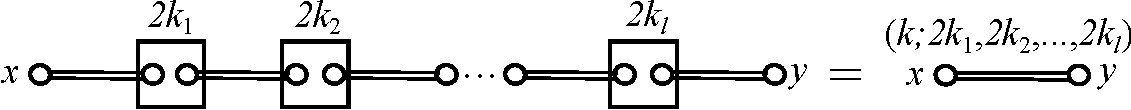
\includegraphics[width=11cm]{Labeldouble.pdf}
	\end{center}
\end{definition}

%\iffalse
%%\begin{remark}
%The scaling order of a labelled $\dashed$ edge is calculated as follows. For \eqref{eq label}, there are $l+1$ $\dashed$ edges of scaling order $2l+2$, $\selfs$ $\Sele _{2k_1},\cdots, \Sele_{2k_l}$ of scaling order $\sum_{i=1}^l 2 k_i$, and $2l$ internal atoms of scaling order $-4l$. Hence the total scaling order is $(2l+2)+\sum_{i=1}^l 2 k_i -4l =k. $
%%As discussed in Remark \ref{lem redagain}, the labelled $\dashed$ edges correspond to propagators with self-energy corrections in Feynman diagrams. 
%By \eqref{BRB}, \eqref{eq label} is bounded by $W^{-(k/2-1)d+\tau}B_{xy}$ for any constant $\tau>0$. Hence it has the same decay with respect to $|x-y|$ as $\Theta_{xy}$ except for an extra $W^{-(k-2)d/2}$ factor. This is the reason why we use it as a $\dashed$ edge. As a convention, whenever we refer to $\dashed$ edges, we mean both the \emph{$\dashed$} and \emph{labelled $\dashed$ edges}. 
%%a $\Theta\Selek_{2l}\Theta$ edge has scaling order $2l$. More precisely, there are two $\dashed$ $\Theta$ edges of scaling order 4, a subgraph $\Selek_{2l}$, and two internal atoms of scaling order $-4$. Hence the total scaling order is $2l$.
%%\end{remark}
%
%As we will show in \eqref{BRB} below, \eqref{eq label} is bounded by $W^{-(k/2-1)d+\tau}B_{xy}$ for any constant $\tau>0$. Hence it has the same decay with respect to $|x-y|$ as $\Theta_{xy}$ (recall \eqref{thetaxy}) except for an extra $W^{-(k/2-1)d}$ factor. This is the reason why we use it as a $\dashed$ edge. As a convention, whenever we refer to $\dashed$ edges, we mean both the $\dashed$ $\Theta$ edges and the labelled $\dashed$ edges. Moreover, the  doubly connected property in Definition \ref{def 2net} can be also extended by including labelled $\dashed$ edges, with the understanding that a labelled $\dashed$ edge can be used either in the blue net or in the black net.
%\fi

In this paper, whenever we refer to $\dashed$ edges, we mean both the $\dashed$ and labelled $\dashed$ edges. The scaling order of a normal regular graph with labelled $\dashed$ edges can be equivalently calculated as
%by regarding athe definition \eqref{eq_deforderrandom2} of scaling order is extended as 
\begin{align}
	\text{ord}(\cal G) &:= \#\{\text{off-diagonal }  G  \text{ edges}\} + \#\{\text{light weights}\} + 2\#\{ \text{waved edges}\}  + 2 \#\{\text{unlabelled $\dashed$ edges}\} \nonumber\\
	&+\sum_k k\cdot   \#\{k\text{-th order labelled $\dashed$ edges}\}  -  2\left[ \#\{\text{internal atoms}\}- \#\{\text{dotted edges}\} \right] .\label{eq_deforderrandom3}
\end{align}
In other words, a $k$-th order labelled $\dashed$ edge is simply counted as an edge of scaling order $k$, and there is no need to count its internal structures using Definition \ref{def scaling}.

\subsection{Molecular graphs and doubly connected property}\label{sec doublenet}
 
Each of our graphs has a two-level structure, that is, a local structure varying on scales of order $W$, and a global structure varying on scales up to $L$. To explain this, we introduce the following concept of molecules. 

%We first introduce the concept of molecules for the graphs defined in Section \ref{unisec}.

\begin{definition}[Molecules]\label{def_poly}
We partition the set of all atoms into a union of disjoint sets $\{\text{all atoms}\}=\cup_j \cal M_j$, where every $\cal M_j$ is called a molecule. Two internal atoms belong to the same molecule if and only if they are connected by a path of neutral/plus/minus \emph{waved edges} and \emph{dotted edges} (such a path may pass through external atoms). % (note there may be dotted edges if the graph is not regular). 
	%For the atoms in the same molecules, we always combine them if they are the same (i.e. if they are connected by a dotted line). %Moreover, we assign a dash-dotted line partition of them, that is each two atoms in the same molecule are connected through a cross dah-dotted edge. We do not assign dah-dotted line partitions to all the graph, that is, atoms in different molecules can be the same (except in some middle steps of the expansions, in which case we will mention it explicitly). 
	Every external atom will be by definition called an external molecule (such as $\otimes$, $\oplus$ and $\ominus$ molecules).  %If $\oplus=\ominus$, then we call the molecule containing them as $\oplus$ molecule. 
	An edge is said to be inside a molecule if its ending atoms belong to this molecule.
\end{definition}
%\begin{remark}
%	Note that by \eqref{compact f} and \eqref{S+xy}, if two atoms are in the same molecule, then we essentially have $$|x-y|\le (\log W)^2 W$$ up to a negligible error $\OO(W^{-D})$ in all the expressions. 
%\end{remark}
By \eqref{subpoly} and \eqref{S+xy}, if two atoms $x$ and $y$ are in the same molecule, then we essentially have $|x-y|\le W^{1+\tau}$ up to a negligible error $\OO(W^{-D})$. Given an atomic graph, we will call the subgraph inside a molecule the {\it local structure} of this molecule. On the other hand, the {\it global structure} of an atomic graph refers to its \emph{molecular graph}, which is the quotient graph with each molecule regarded as a vertex. 
%We call the structure of the molecular graph the {\it global structure}.  \hty{ The {\it global structure} of a graph is by definition the molecular graph}
%Corresponding to each atomic graph, we can define a molecular graph, whose vertices are molecules.
%\iffalse
%\begin{definition}[Molecular graphs] \label{def moleg}% \cob (need details) \nc 
%	Molecular graphs are graphs consisting of 
%	\begin{itemize}
%		\item external molecules which represent the external atoms (such as the $\otimes$, $\oplus$ and $\ominus$ molecules);
%		\item the internal molecules;
%		\item blue solid edges, which represent plus $G$ edges between molecules;
%		\item $\dashed$ %and labelled $\dashed$ 
%		edges between molecules;
%		\item dotted edges between pairs of external and internal molecule.
%		%  \item dots are molecules
%		% \item only has blue edges
%		%\item No inside information of molecule, (\cob we can also leave the local information of blue edges in molecule-level graphs.\nc)  
%	\end{itemize}
%	%  \end{definition}
%	%\begin{definition}  \nc  
%	For any atomic graph $\cal G$, we define its molecular version, called $ \cal G_{\cal M}$, in the following way:
%	\begin{itemize}
%		\item each molecule in $\cal G$ is represented by a vertex in $ \cal G_{\cal M}$;
%		
%		\item each solid blue edge (i.e. plus $G$ edge) between atoms in two molecules is represented by a solid blue edge between these two molecules in $ \cal G_{\cal M}$;
%		
%		\item each solid blue edge inside a molecule becomes a self-loop on this molecule in $ \cal G_{\cal M}$;
%		
%		\item each $\dashed$ edge between atoms in two molecules is represented by a $\dashed$ edge between these two molecules in $ \cal G_{\cal M}$;
%		
%		\item each dotted edge between a pair of external and internal atoms is represented by a dotted edge between the corresponding external and internal molecules;
%		
%		%\item if there are multiple $\times$-dotted lines between the same pair of molecules, then we only keep one of them; 
%		%{\it dotted line} between them, which means that there are at least a pair of atoms in these two molecules that always take the same value;
%		
%		\item we discard all the other components in $\cal G$ (including the weights, $\times$-dotted lines, red solid $\overline G$ edges, and the waved and $\dashed$ edges inside molecules). %to $ \cal G_{\cal M}$.
%	\end{itemize}
%	%  \noindent{\bf Simple level 2 standard graphs:} We now introduce a strange trick, that is, we only keep the blue solid edges in the graphs and for the red solid edges we only record the total number of them. More precisely, corresponding to a standard graph $\cal G$, we define the simple standard graph $S(\cal G)$ as the subgraph with only black and grey $\dashed$ edges and blue solid $G$ edges. Note that we will expand the graph $\cal G$ only, and $S(\cal G)$ is used to help to study the molecule family tree structure. (\cor draw an example\nc) 
%\end{definition}
%\fi

\begin{definition}[Molecular graphs] \label{def moleg}% \cob (need details) \nc 
 Molecular graphs are graphs consisting of 
	\begin{itemize}
		\item external molecules which represent the external atoms (such as the $\otimes$, $\oplus$ and $\ominus$ molecules);
		\item internal molecules;
		\item blue and red solid edges, which represent the plus and minus $G$ edges between molecules;
		\item $\dashed$ edges between molecules;
		\item dotted edges between external and internal molecules.
		%  \item dots are molecules
		% \item only has blue edges
		%\item No inside information of molecule, (\cob we can also leave the local information of blue edges in molecule-level graphs.\nc)  
	\end{itemize}
	%  \end{definition}
	%\begin{definition}  \nc  
	Given any atomic graph $\cal G$, we define its molecular version, called $ \cal G_{\cal M}$, in the following way:
	\begin{itemize}
		\item every molecule of $\cal G$ is represented by a vertex in $ \cal G_{\cal M}$;
		
		\item every blue or red solid edge of $\cal G$ between atoms in different molecules is represented by a blue or red solid edge between these two molecules in $ \cal G_{\cal M}$;
		
		\iffalse
		\item each solid blue edge inside a molecule becomes a self-loop on this molecule in $ \cal G_{\cal M}$;
		\fi
		
		\item every $\dashed$ edge of $\cal G$ between atoms in different molecules is represented by a $\dashed$ edge between these two molecules in $ \cal G_{\cal M}$;
		
		\item every dotted edge of $\cal G$ between an external atom and an internal atom is represented by a dotted edge between the corresponding external and internal molecules;
		
		%\item if there are multiple $\times$-dotted lines between the same pair of molecules, then we only keep one of them; 
		%{\it dotted line} between them, which means that there are at least a pair of atoms in these two molecules that always take the same value;
		
		\item we discard all the other components in $\cal G$ (including weights, $\times$-dotted edges, and edges inside molecules).
	\end{itemize}
	The molecules are determined by the graph $\cal G$ with all its dotted edges. A dotted edge between an internal atom $X$ and $\fb_1$ (resp.~$\fb_2$) inherits the color of the solid edge that it replaces, that is, it is regarded as a blue (resp.~red) solid edge between the molecule containing $X$ and $\fb_1$ (resp.~$\fb_2$). More precisely, a dotted edge at $\fb_1$ is counted as a blue solid edge between a subset of molecules and its complement (as in Definition \ref{defn iso} below), but it is not used in the blue net of Definition \ref{def 2net} or in a pre-deterministic order (see Definition \ref{def PDG} below); a dotted edge at $\fb_2$ is removed together with the red solid edges, and it is counted as a red solid edge between a subset of molecules and its complement when we determine whether an isolated subgraph is weakly isolated (see Definition \ref{def_weakstrong} below). Moreover, if an internal atom $X$ is identified with $\fb_1$ or $\fb_2$ through a dotted edge, then all edges at $\fb_1$ or $\fb_2$ are regarded as edges at $X$.

	We say that an external atom is \emph{identified} if it is connected to an internal atom by a dotted edge, and \emph{unidentified} otherwise. We say that a graph satisfies \emph{condition (E)} if the following properties hold: there is no dotted or $\times$-dotted edge between two unidentified external atoms; if $\fa$ is unidentified, then it is connected to a $\dashed$ edge whose other end is an internal or identified atom, and to no $\dashed$ edge whose other end is an unidentified atom; if $\fb_2$ is unidentified, then it is connected to no $\dashed$ edge and to at most one solid edge; if $\fb_1$ is unidentified, then it is connected to a blue solid edge or to a $\dashed$ edge whose other end is an internal or identified atom, to no $\dashed$ edge whose other end is an unidentified atom, and to at most one solid or $\dashed$ edge in total. Condition (E) is needed in Lemmas \ref{lem localgood2} and \ref{lem localgoodQ} below.
	%  \noindent{\bf Simple level 2 standard graphs:} We now introduce a strange trick, that is, we only keep the blue solid edges in the graphs and for the red solid edges we only record the total number of them. More precisely, corresponding to a standard graph $\cal G$, we define the simple standard graph $S(\cal G)$ as the subgraph with only black and grey $\dashed$ edges and blue solid $G$ edges. Note that we will expand the graph $\cal G$ only, and $S(\cal G)$ is used to help to study the molecule family tree structure. (\cor draw an example\nc) 
\end{definition}

%Note that the local structures can only vary on scales of order $\OO (W^{1+\tau})$, while the global structure varies on scales up to  $L$. The \emph{two-level structure} of an atomic graph---a global structure plus several local structures---has been explored in \cite{PartIII} already. 

%\cor
%We will only expand the atomic graphs, and the molecule-level-graphs is used solely to help with the analysis of the graph structures. In the proof, we assume that for each atomic graph we automatically have a molecular graph associated with it. Note that we do not keep the red solid $\overline G$ edges in the molecular graphs. This is because we want to keep the molecular graph as concise as possible, so that we can focus on the structures of the $\dashed$ and plus $G$ edges. 
%\nc

In this paper, molecular graphs are used solely to help with the analysis of graph structures, while all graph expansions are  applied to atomic graphs only. In the proof, we assume that there is automatically a molecular graph associated with each atomic graph. In general, local structures are almost trivial to bound, while global structures are much harder to analyze. This is one of the main reasons why we want to introduce the concept of molecular graphs---we want to get rid of all local structures and focus on the more intricate global structures instead.



%\begin{remark}
%Note that the dotted-line partition of the molecular graph is not necessary consistent. For example, there may be a $G$ edge between two molecules, which is accompanied by a $\times$-dotted line. On the other hand, there may be a dotted edge between the other two atoms in these molecules, and we keep both of them, because, as we said above, the molecule-level-graphs will only be used to help with the analysis.
%\end{remark}

%  \begin{definition}[$\Theta$-expansion $\cal O_\theta(x)$]     
%% \cob (need details) \nc 
%%  [Operator for charged atoms $\cal O_e^{(2)}(x)$:] 
%Given a level 1 standard graph $\cal G$, suppose for some standard neutral atom $x$, it is connected to an $s_{wx}$ edge, two $G$ edges of opposite charges and has no weights. Suppose the graph takes the form $|m|^2\sum_x s_{wx}G_{xy}   \overline G_{xy' }  f(G)$ with $x\notin \{y,y'\}$. Then we have
%\begin{align}
%& \cal O_\theta(x)\left[|m|^2\sum_x s_{wx}G_{xy}   \overline G_{xy' }  f(G)\right] = %m\delta_{xy} G_{y' y} f(G) + 
%m  \Theta_{wy}  \overline G_{yy'} f(G)  \nonumber\\
%&+ m\sum_{\al,\beta} \Theta_{w\al} s_{\al\beta} (G_{\beta\beta}-m) G_{\al y} \overline G_{\al y'} f(G) + m \sum_{\al,\beta} \Theta_{w\al} s_{\al\beta}  ( \overline G_{\al\al } -\overline m) G_{\beta y}\overline G_{\beta y'}  f(G) \nonumber \\
%& - m \sum_{\al,\beta} \Theta_{w\al} s_{\al\beta}G_{\beta y} \overline G_{\al y'} \partial_{\overline h_{\al\beta}}f(G)  +\cal Q_\theta \label{Otheta},
% \end{align}
% where
%\begin{align*}
%    & \cal Q_\theta:= |m|^2 \sum_x s_{wx}Q_x\left[G_{xy}   \overline G_{xy' }  f(G)\right]  - m  \Theta_{wy} Q_y( \overline G_{yy'} f(G) ) + m \sum_{\al,\beta} \Theta_{w\al} s_{\al\beta}Q_\al\left[G_{\beta y} \overline G_{\al y'} \partial_{\overline h_{\al\beta}}f(G) \right] \nonumber\\
%    &-  m\sum_{\al,\beta} \Theta_{w\al} s_{\al\beta} Q_\al\left[(G_{\beta\beta}-m) G_{\al y} \overline G_{\al y'} f(G)\right] - m \sum_{\al,\beta} \Theta_{w\al} s_{\al\beta} Q_\al\left[ ( \overline G_{\al\al } -\overline m) G_{\beta y}\overline G_{\beta y'}  f(G) \right].
% \end{align*}
%%Similarly, $\cal O_e^{(2)}(x)[ G_{yx}  \overline G_{y' x }  f(G)]$ can be defined easily by taking complex conjugate. 
%For the reason of the above definition, we refer to Lemma \ref{T eq} below (note that $|m|^2S\theta=\Theta$).
%  \end{definition}

%We now check the orders of the graphs on the RHS of the expansions. First, if $y\ne y'$, then all the graphs in the first two lines on the right-hand side of \eqref{Otheta} are at least one order higher than the original graph. If $y'=y$, then the leading term is  
%\be\label{Othetaleading}m  \Theta_{wy}  \overline G_{yy} f(G),\ee
%which has the same order as the original graph, while the rest of the graphs in the first two lines on the right-hand side of \eqref{Otheta} are at least one order higher than the original graph. 


%----------Jun's notes------------ 
%\begin{definition}  \cob (need details) \nc Some operators on molecule-level-graph
%\begin{enumerate}
%\item Pulling-operators on molecule-level-graph, $\cal O^\cal M_P(\Gamma, \al)$ is a set of molecule-level graphs. 
%\item Create new molecule
%\end{enumerate}
%
%  \end{definition}
%\begin{lemma}
%The effort of operator ${\cal O}_{weight}$,  $\cal O_e$ and  $\theta$-expansion on Molecule-level-graph.    \cob (need details) \nc 
%In this lemma, we describe efforts of these operators. For example, for  $\Gamma$ with  $ (\Gamma)_{\cal M}$, and $\alpha$ is a atom in $\Gamma$, we know 
%$$\left({\cal O}_{weight} (\Gamma, \al) \right)_{\cal M}
%$$
%has the following properties.    \cob (need details)
%\end{lemma}
%---------------------------------------

%\begin{remark}
%We shall call the subgraph inside a molecule (i.e. the subgraph consists of the atoms inside this molecule and the edges between them) a {\it local structure}. On the other hand, we shall call the structure of the molecular graph the {\it global structure}. Note that the local structures can only vary on scales of order $\OO_\prec(W)$, while the global structure varies on the scale $L$. In general, the global structure is much harder to analyze than the local structures, which is one of the main reasons why we want to introduce the molecular graph.
%\end{remark}

%The following \emph{double-net (or doubly connected) property} is crucial for our proof, because it allows us to establish a direct connection between the scaling order of a graph and a bound on its value (cf. Lemma \ref{no dot} and Lemma \ref{general dot} below).  We want our graphs in $T$-expansions to satisfy this property. We emphasize that the double-net property is defined on the molecular graphs, and hence we will say that it is a \emph{global property}.
%
%\begin{definition} [Double-net/doubly connected property]\label{def 2net}  %\cob details are needed \nc. 
%	Given a graph or subgraph $\cal G$ without external molecules, we say $\cal G$ is {\bf doubly connected} or has a {\bf double-net} if its molecular graph $\cal G_{\cal M}$ satisfies the following property. There exist a collection, say $\cal B_1$, of $\dashed$ edges, and another collection, say $\cal B_2$, of blue solid (i.e. plus $G$) and $\dashed$ edges, such that (a) $\cal B_1\cap \cal B_2=\emptyset$, and (b) each of $\cal B_1$ and $\cal B_2$ is a connected subset of edges that connect all the molecules in $\cal G_{\cal M}$. For simplicity of notations, we sometimes call the $\dashed$ edges in $\cal B_1$ as black edges, and the blue solid and $\dashed$ edges in $\cal B_2$ as blue edges. Correspondingly, $\cal B_1$ and $\cal B_2$ are referred to as black net and blue net, respectively.  
%	
%	On the other hand, given a graph $\cal G$ with external molecules, we say $\cal G$ is doubly connected if the subgraph $\cal G_0$ of $\cal G$ obtained by removing the external molecules is doubly connected.
%	%(\cor two systems of spanning trees, disconnected\nc)
%	%We shall call a collection of edges ``a net" if these edges connect all the normal molecules except $\oplus$ and $\otimes$ (i.e. the graph with the normal molecules and the collection of edges is edge connected). We say a graph is a double nets graphs if it has two disjoint nets, where one net consists of black or grey $\dashed$ edges only and the other consists of black dashed, grey dashed or blue solid edges. 
%	% {\bf Important:} Of course, the 2net concept is correct. But in most calculation/application, the form we used is the one with 1 external black edge and 1 black/blue edge. Therefore, one should introduce a concept i.e., 2net with 2 external edges. The main reason is 
%	% 1: black external edge will be used in summation 
%	% 2: blue external edge will be used in expansion. 
%	% \cob Overall, we need to change from 2net to 2net+2external
%\end{definition}
%\begin{remark}
%We have defined the double-net property in a way such that after combining the molecules that are connected through dotted edges, the following property holds. There exist two collections of edges, $\cal B_1$ of black $\dashed$ edges and $\cal B_2$ of blue $\dashed$ and plus $G$ edges, such that $\cal B_1\cap \cal B_2=\emptyset$ and each of them 
% is a subset of edges that connect all the molecules together. Hence there are two distinct connected nets of edges in the graph, which explains the name ``double-net" and ``doubly connected".
%\end{remark}


The following \emph{doubly connected property} is crucial for our proof, because it allows us to establish a direct connection between the scaling order of a graph and a bound on its value. All graphs in the $T$-expansion and $\incomp$ will satisfy this property (cf. Definitions \ref{defn genuni} and \ref{def incompgenuni}). 

\begin{definition} [Doubly connected property]\label{def 2net}  %\cob details are needed \nc. 
A subgraph $\cal G$ without external molecules is said to be doubly connected if its molecular graph $\cal G_{\cal M}$ satisfies the following property. There exists a collection, say $\cal B_{black}$, of $\dashed$ edges, and another collection, say $\cal B_{blue}$, of  either blue solid or  $\dashed$ edges  such that (a) $\cal B_{black}\cap \cal B_{blue}=\emptyset$, and (b) both $\cal B_{black}$ and $\cal B_{blue}$ contain a spanning tree that connects all molecules in the graph. For simplicity of notations, we call the $\dashed$ edges in $\cal B_{black}$ as black edges, and the blue solid and $\dashed$ edges in $\cal B_{blue}$ as blue edges. Correspondingly, $\cal B_{black}$ and $\cal B_{blue}$ are referred to as black net and blue net, respectively, where a ``net" refers to a subset of edges that contains a spanning tree (if there is at most one molecule, this condition holds trivially).

A graph $\cal G$ with external molecules is called doubly connected if its subgraph with all external molecules removed is doubly connected,  i.e. the spanning trees in the two nets are not required to contain the external molecules.
\end{definition}
%\begin{remark}
%We emphasize that the double-net property is defined on the molecular graphs, so it is a \emph{global property}. In the above definition, the $\dashed$ edges also include the labelled $\dashed$ edges introduced in Definition \ref{def_graph comp}.  
%the double-net property in Definition \ref{def 2net} can be also extended by including labelled $\dashed$ edges, with the understanding that a labelled $\dashed$ edge can be used either in the blue net or in the black net.
Note that red solid edges are not tracked in the doubly connected property. In fact, the connectivity of red solid edges will be broken in our expansion procedures. Hence we will often consider molecular graphs with all red solid edges removed. % see Section \ref{sec pre} below. %In other words, in the graphs from the expansions of the $T$-variables, we generally {\bf do not} have a collection $\cal B_{black}$ of $\dashed$ edges and another disjoint collection $\cal B_{red}$ of red solid and $\dashed$ edges, so that both of them are connected subset of edges that connect all molecules. %However, a weaker double-net property holds: if we split each $\dashed$ edge into a blue solid edge and a red solid edge, then there is a connected blue net of blue solid edges and a  connected red net of red solid edges in the graph. This property is weaker than the double-net property in Definition \ref{def 2net}.
%For the graphs in $T$-expansions, they are all doubly connected in the sense of Definition \ref{def 2net} if we remove the external molecules $\oplus$, $\ominus$ and $\otimes$ (together with the edges connected to them).
Doubly connected graphs satisfy some important bounds that depend explicitly on their scaling orders; see Lemma \ref{no dot} below. 





%\begin{remark}
%Here the two external edges refers to the fact that: there is at least one blue edge between the internal molecules and $\ominus$, and at least one black edge between the internal molecules and $\oplus$. Roughly speaking, the black external edge will be used in summation, and the blue external edge will be used in expansion (if it is a $G$ edge). 
%\end{remark}

%For a doubly-connected graph, we can use its scaling order defined algebraically in \eqref{eq_deforderrandom2} to give an estimate on its graph value as we will show in Lemma \ref{general dot}. This is the main reason why we want to keep the doubly connected property for all the graphs. 









\section{Main results}\label{sec outline}

%\subsection{Proof of Theorem \ref{main thm}.}\ 
%\noindent{\underline{\bf (I) $T$-expansions.}} 

In this section, we define the concepts of $T$-expansion and $\incomp$, which were introduced in \cite[Section 2]{PartI_high}. 
Then we will state our main results in Section \ref{subsec_main}. In this paper, we will focus on expansions of the $T$-variable $T_{\fa,\fb_1 \fb_2}$, while expansions of $T_{\fb_1\fb_2,\fa}$ can be obtained immediately by considering the transposition of $T_{\fa,\fb_1 \fb_2}$.
%from which we can immediately obtain the corresponding $T$-expansions for $T_{yy',x}$ by replacing $G$ with $G^\top$ in all the expressions.
 

\subsection{$T$-expansion}\label{sec Texp2}


In this subsection, we define the $T$-expansion using the notations introduced in Section \ref{sec notation}. In addition, we also introduce the following two types of graphs. 
 
\begin{definition}[Recollision graphs and $Q$-graphs]\label{Def_recoll}
(i) We say a graph is a $\oplus$/$\ominus$-recollision graph, if there is at least one dotted edge connecting $\oplus$ or $\ominus$ to an internal atom. In other words, a recollision graph represents an expression where we set at least one summation index to be equal to $\fb_1$ or $\fb_2$.
 	
\medskip
\noindent(ii) We say a graph is a $Q$-graph if it contains at least one $Q$ label, and all  $G$ edges and $G$ weights in the graph (together with all the other random factors introduced later, such as $G^{(x)}$ entries, $(G_{xx})^{-1}$ weights and $\cal W^{(x)}_{D}$ weights in Section \ref{sec defnQ}) have the same $Q_x$ label with a specific atom $x$, i.e., %all $Q$ operators
all $Q$ labels in the graph are the same $Q_x$ for some atom $x$. In other words, the value of a $Q$-graph can be written as $Q_x(\Gamma)$ for an external atom $x$ or $\sum_x Q_x(\Gamma)$ for an internal atom $x$, where $\Gamma$ is a graph without $Q$ labels. 
\end{definition}
 
 
For any $n\in \N$, we now define the $n$-th order $T$-expansion. Its graphs actually satisfy several more delicate properties to be stated later in %Definition \ref{def genuni} and 
Definition \ref{def genuni2}. 



\begin{definition} [$n$-th order $T$-expansion]\label{defn genuni}
	%For any fixed order $n$, suppose we have defined the sequence of deterministic graphs $S^{(k)}_ \Delta$, $2\le k \le n-1$. Then 
	Fix any $n\in \N$ and a large constant $D\ge n+2$. For $\fa, \fb_1,\fb_2 \in \Z_L^d$, an $n$-th order $T$-expansion of $T_{\fa,\fb_1\fb_2}$ with $D$-th order error is an expression of the following form: %for any fixed large constant $D>0$,
	%\be\label{mlevelTgdefintro}
	%T_{xy}= |m|^2  \Theta_{xy} +|m|^2   \left(\Theta \Sdelta^{(n)} \Theta\right)_{xy}  + (\PTn)_{xy} +  (\ATn)_{xy} + (\QTn)_{xy} . %+ \OO_\prec(W^{-D})
	%\ee
	\be\label{mlevelTgdef}
	\begin{split}
		T_{\fa,\fb_1 \fb_2}&= m  \Theta_{\fa \fb_1}\overline G_{\fb_1\fb_2} +m   (\Theta \Sdelta^{(n)}\Theta)_{\fa\fb_1} \overline G_{\fb_1\fb_2} \\
		&+ (\PTn)_{\fa,\fb_1 \fb_2} +  (\ATn)_{\fa,\fb_1\fb_2}  + (\QTn)_{\fa,\fb_1\fb_2}  +  (\Err_{n,D})_{\fa,\fb_1\fb_2}.
	\end{split}
	\ee
	The graphs on the right side depend only on $n$, $D$, $m(z)$, $S$, $S^{\pm}(z)$, $\Theta(z)$ and $G(z)$, but do not depend on $W$, $L$ and $d$ explicitly. Moreover, they satisfy the following properties with $C_n$ and $C_D$ denoting large constants depending on $n$ and $D$, respectively.
	\begin{enumerate}
		\item  The graphs on the right side are normal regular graphs (recall Definition \ref{defnlvl0}) with external atoms $\otimes\equiv \fa$, $\oplus\equiv \fb_1$ and $\ominus\equiv \fb_2$, and with at most $C_D$ many atoms. Their dotted edges contain no cycles (recall Definition \ref{def scaling}).
		%Moreover, the expressions on the right-hand side satisfy the following properties.  
		
		\item %The graphs on the right-hand side of \eqref{mlevelTgdef} may contain labelled $\dashed$ edges of the form \eqref{eq label}, where we must have that $4\le 2k_i \le n-1$ and $k=\sum_{i=1}^l 2 k_i -2(l-1)\le n-1$. In other words, the definition of the $n$-th order $T$-expansion only uses lower order $\selfs$.
		A diffusive edge in any graph on the right-hand side of \eqref{mlevelTgdef} is either a $\dashed$ edge or a labelled $\dashed$ edge of the form \eqref{eq label} with $4\le 2k_i \le n$.
		
		\item $\Sdelta^{(n)}$ is a sum of at most $C_n$ many deterministic normal regular graphs. %of $m(z)$, $I_N$, $S$, $S^\pm(z)$ and $\Theta(z)$ only. 
		We decompose it according to the scaling order as 
		\be\label{decompose Sdelta0} \Sdelta^{(n)} = \sum_{k\le n} \Sdeltak.\ee
		%where each $\Sdelta_{k}$ is a sum of deterministic graphs of scaling order $k$. 
		Moreover, we have a sequence of $\selfs$ $\Sele_{k}$ satisfying Definition \ref{collection elements} for $4\le k \le n$ such that $\Sdeltak$ can be written into the form %of chain structures: 
		\be\label{chain S2k}
		\Sdeltak=\Sele_{k} + \sum_{ l =2}^k \sum\limits_{ \mathbf k=(k_1,\cdots, k_l) \in \Omega_{k}^{(l)} } \Sele_{k_1}\Theta  \Sele_{k_2}\Theta \cdots \Theta  \Sele_{k_l} . %\mathbf 1\left(\mathbf k \in \Omega_{k}^{(l)}\right).
		\ee
		%where $\Sele_{k}\in \Cele_{k}$ for $2\le k \le n-1$ and $\Sele_{k_i} \in \Cele_{k_i}$. 
		Here all deterministic graphs with $l=1$ are included into $\Sele_k$ so that the summation starts with $l=2$. Moreover,  $\Omega_{k}^{(l)} \subset \N^l$ is the subset of vectors $\mathbf k$ satisfying that 
		\be\label{omegakl}
		4\le k_i \le k-1,\quad \text{ and }\quad  \sum_{i=1}^l  k_i  -2(l-1)=k. 
		\ee
		%$ \Omega_{k}^{(l)} \subset \N^l$ is a subset of vectors such that every $ \mathbf k \in \Omega_{k}^{(l)} $ satisfies %\eqref{omegakl},  
		%\be\label{omegakl}
		% 4\le k_i \le k-1,\quad \text{ and }\quad \left(\sum_{i=1}^l  k_i\right) -2(l-1)=k, 
		% \ee
		The second condition of \eqref{omegakl} guarantees that the subgraph $(\Sele_{k_1}\Theta  \Sele_{k_2}\Theta \cdots \Theta  \Sele_{k_l})_{xy}$ has scaling order $k$.
		%But we remark that $ \Omega_{k}^{(l)}$ does not necessarily contain all possible vectors $\mathbf k\in \N^l$ that satisfy \eqref{omegakl}.
		%${\bm \kappa}=(\kappa_1,\cdots, \kappa_l)$ is a sequence of labels for the expressions $\Sele_{k_i}$, $1\le i \le l$ (as an additional remark, $\kappa_i$ does not necessarily range over all the elements in $\Cele_{k_i}$). 
		%Finally, the deterministic expression $\Sele_{n}$ satisfies the properties (i)-(iii) of Definition \ref{collection elements}.  %and we include it into the set $\Cele_n$.  
		%for each fixed $l\in \N$, there are at most $C_l$ many labels $\kappa$ for $\Selek_{2l}$, and as a convention, we regard the label of $\Sele_{2k}$ as $\emptyset$.
		
		
		\item $(\PTn)_{\fa,\fb_1\fb_2}$ is a sum of at most $C_n$ many $\oplus/\ominus$-recollision graphs of scaling order $\le n$ and without any $P/Q$ labels.  Moreover, it can be decomposed as 
		\be\label{decomposeP}(\PTn)_{\fa,\fb_1\fb_2} =\sum_{ k =3}^{ n}(\PTk)_{\fa,\fb_1\fb_2},\ee
		where each $(\PTk)_{\fa,\fb_1\fb_2}$ is a sum of the $\oplus/\ominus$-recollision graphs of scaling order $k$ in $(\PTn)_{\fa,\fb_1\fb_2}$. 
		
		
		\item  $(\ATn)_{\fa,\fb_1\fb_2}$ is a sum of at most $C_D$ many graphs of scaling order $> n$ and without any  $P/Q$ labels.  
		
		
		\item $(\QTn)_{\fa,\fb_1\fb_2} $ is a sum of at most $C_D$ many $Q$-graphs.  Moreover, it can be decomposed as 
		\be\label{decomposeQ} (\QTn)_{\fa,\fb_1\fb_2}= \sum_{k=2}^{n} (\QTk)_{\fa,\fb_1\fb_2} + (\cal Q^{(>n)}_T)_{\fa,\fb_1\fb_2},\ee
		where  $(\QTk)_{\fa,\fb_1\fb_2}$ is a sum of the $Q$-graphs in $ (\QTn)_{\fa,\fb_1\fb_2}$ of scaling order $k$, and $(\cal Q^{(>n)}_T)_{\fa,\fb_1\fb_2}$ is a sum of all the $Q$-graphs in $ (\QTn)_{\fa,\fb_1\fb_2}$ of scaling order $>n$.
		
		
		
		\item $\Sdeltak$, $\PTk$ and $\QTk$ are independent  of $n$.
		
		\item $(\Err_{n,D})_{\fa,\fb_1\fb_2}$ is a sum of at most $C_D$ many graphs, each of which has scaling order $> D$ and may contain some $P/Q$ labels in it, where all the $P/Q$ labels in a graph are the same $P_x$ or $Q_x$ label for an atom $x$. Moreover, every graph in $(\Err_{n,D})_{\fa,\fb_1\fb_2}$ or $(\QTn)_{\fa,\fb_1\fb_2}$ that contains internal atoms has an internal atom connected to $\otimes$, $\oplus$ or $\ominus$ through a waved, $\dashed$ or dotted edge.

		\item In every graph of $(\PTn)_{\fa,\fb_1\fb_2}$, $(\ATn)_{\fa,\fb_1\fb_2}$, $(\QTn)_{\fa,\fb_1\fb_2} $ and $(\Err_{n,D})_{\fa,\fb_1\fb_2}$,  there is a unique $\dashed$ edge connected to $\otimes$, and there is no other edge or weight on $\otimes$. Furthermore,  there is at least an edge, which is either blue solid or $\dashed$ or dotted,  connected to  $\oplus$, and there is at least an edge, which is either red solid or $\dashed$ or dotted,  connected to $\ominus$.

		\item[(ix$'$)] In every graph of $(\ATn)_{\fa,\fb_1\fb_2}$, $(\QTn)_{\fa,\fb_1\fb_2}$ and $(\Err_{n,D})_{\fa,\fb_1\fb_2}$ that has an internal atom and in which neither $\oplus$ nor $\ominus$ is connected to an internal atom by a dotted edge, the $\dashed$ edge at $\otimes$ ends at an internal atom, $\oplus$ is connected to an internal atom by a blue solid or $\dashed$ edge, and $\ominus$ is connected to an internal atom by a red solid or $\dashed$ edge.

		\item Every graph in $(\PTn)_{\fa,\fb_1\fb_2}$, $(\ATn)_{\fa,\fb_1\fb_2}$, $(\QTn)_{\fa,\fb_1\fb_2}$ and $(\Err_{n,D})_{\fa,\fb_1\fb_2}$ is doubly connected in the sense of Definition \ref{def 2net}. 
		
		%Furthermore, there may be some dotted edges connected with $\oplus$ and $\ominus$. 
		
		%\iffalse
		%\item $(\PTn)_{xy}$ is a sum of at most $C_n$ many recollision graphs of scaling order $\le n$: 
		% $$(\PTn)_{xy} =\sum_{k=3}^{ n}(\PTk)_{xy},$$
		% where each $(\PTk)_{xy}$ is a sum of recollision graphs of scaling order $k$. Here a recollision graph means that there is at least one dotted edge connecting the external vertex $y$ to an internal vertex in the graph. In other words, a recollision graph represents an expression where we set at least one summation index to be equal to $y$.
		% %some summation indices in the expression of $(\PT_l)_{xy}$ are equal to the fixed indices $x$ or $y$ {\cor(check this sentence)}.
		%\item $(\ATn)_{xy}$ is a sum of at most $C_n$ many higher order graphs with scaling order $> n$. 
		%
		%\item $(\QTn)_{xy}$ is a sum of at most $C_n$ many $Q$-graphs. Here a $Q$-graph means a fluctuation expression of the form $\sum_\al Q_\al (\Gamma(\al))$ for a graph $\Gamma$ and an internal vertex $\al$ in $\Gamma$, where we denote $Q_\al:=1-\mathbb E_\al$ with $\E_\al[\cdot]$ being the partial expectation over the $\al$-th row and column of $H$.
		%Moreover, we can write %decompose $\QTn$ as 
		%$$ (\QTn)_{xy}= \sum_{k=2}^{n} (\QTk)_{xy} + (\cal Q^{(>n)}_T)_{xy},$$
		%where each $(\QTk)_{xy}$ is the sum of $Q$-graphs of scaling order $k$ in $(\QTn)_{xy}$, and $(\cal Q_T^{(>n)})_{xy}$ is the sum of all the $Q$-graphs of scaling order $>n$ in $(\QTn)_{xy}$.
		% \fi
		
	\end{enumerate}
	The graphs on the right-hand side of \eqref{mlevelTgdef} satisfy some additional properties given in Definition \ref{def genuni2} below. %and Definition \ref{def genuni2}.
\end{definition}


% \begin{remark}\label{lem redagain}
% We make the following remarks regarding the above definition.
%
%\vspace{5pt}
%\noindent{(i)} 

%\iffalse
%In Definition \ref{defn genuni}, the graph $\Selek_{l}$ can be regarded as a sum of irreducible graphs (in the sense of Definition \ref{def 2net} below). Then the graphs in $\Sdeltak$ are formed by connecting the irreducible graphs with $\Theta$ edges. We also remark that in accordance with \eqref{trivial conv}, we have
% $$\Sigma_1=\Sigma_2=\Sigma_3=\Sigma_{2l+1}=0,\quad l\in \N.$$
%\fi
% \end{remark}
% \begin{remark}


%\vspace{5pt}
%\noindent{(ii)} One of the leading graphs in $(\cal P_{T,3})_{xy}$ is 
%$$m \sum_{\al,\beta} \delta_{\al y}\Theta_{x\al} s_{\al\beta}  ( \overline G_{\al\al } - \overline m) |G_{\beta y}|^2 ,$$
%which can be easily bounded by $\Theta_{xy}$ if we have a rough estimate on $G$ as in \eqref{initialGT}. In general, there are many more complicated graphs in $\PTn$, but they are all sufficiently small for our purpose. 
% \end{remark}
% \begin{remark}


% \vspace{5pt}
%\noindent{(iii)} 
%Compared with \eqref{sum S2l}, the estimate \eqref{3rd_property0} is much stronger by an extra $\eta$ factor, which actually follows from the sum zero property \eqref{weaz} and is crucial for our proof. In particular, 


By \eqref{BRB}, the term $\left(\Theta \Sdeltak \Theta\right)_{\fa\fb_1}$ can be bounded as 
\be\label{intro_redagain}|\left(\Theta \Sdeltak \Theta\right)_{\fa\fb_1} |\le W^{-(k-2)d/2+\tau}B_{\fa\fb_1} \ee
for any constant $\tau>0$. This bound shows that when $\fb_1=\fb_2=\fb$, the second term on the right-hand side of \eqref{mlevelTgdef} can be bounded by  $m\overline G_{\fb\fb}(\Theta \Sdelta^{(n)} \Theta)_{\fa\fb}=\OO(W^\tau B_{\fa\fb})$, which is necessary for the local law \eqref{locallaw} to hold.


In \cite{PartI_high}, the following second order $T$-expansion is given explicitly in Lemma 2.5: 
\begin{align}\label{seconduniversal}
	& T_{\fa,\fb_1\fb_2}= %m\delta_{xy} G_{y' y} f(G) + 
	m \overline G_{\fb_1\fb_2}  \Theta_{\fa\fb_1}   + (\AT^{(>2)})_{\fa,\fb_1\fb_2} + (\QT^{(2)})_{\fa,\fb_1\fb_2}  ,
\end{align}
where 
\begin{align}
	(\AT^{(>2)})_{\fa,\fb_1\fb_2}& :  =  m\sum_{x,y} \Theta_{\fa x} s_{xy} (G_{yy}-m) G_{x \fb_1}\overline G_{x \fb_2}  + m \sum_{x,y} \Theta_{\fa x} s_{xy}  ( \overline G_{xx} - \overline m) G_{y \fb_1}\overline G_{y \fb_2}, \label{Aho>2}  \\
	(\QT^{(2)})_{\fa,\fb_1\fb_2}& := \sum_x Q_x\left(\Theta_{\fa x} G_{x \fb_1}   \overline G_{x \fb_2} \right) - m Q_{\fb_1} \left( \Theta_{\fa\fb_1} \overline G_{\fb_1 \fb_2}\right)  \nonumber\\
	& -  m\sum_{x,y} Q_x\left[\Theta_{\fa x} s_{xy} (G_{yy}-m) G_{x \fb_1} \overline G_{x \fb_2} \right] - m \sum_{x,y} Q_x\left[ \Theta_{\fa x} s_{xy}  \overline G_{xx} G_{y\fb_1}\overline G_{y\fb_2} \right] .\label{QT>2}
\end{align}
We still need to expand $(\AT^{(>2)})_{\fa,\fb_1\fb_2}$ and $(\QT^{(2)})_{\fa,\fb_1\fb_2} $ into sums of normal regular graphs using the operation in Definition \ref{dot-def} below, but we omit this minor issue here. 

\subsection{$\incomp$}

%We now extend Definition \ref{defn genuni} to the $T$-expansions of generalized $T$-variables \eqref{general_T}. Moreover, we will state more detailed properties on the graphs. Even more details will be added later in Definition \ref{def genuni2}. For the definition, we introduce the following two types of graphs. 
%\begin{definition}
%	%\begin{itemize}
%	
%	%\item[(I)] 
%	(i) We say a graph is a $\oplus$/$\ominus$-recollision graph, if there is at least one dotted edge connecting $\oplus$/$\ominus$ to an internal atom. 
%	
%	\medskip
%	\noindent(ii) We say a graph is a $Q$-graph if all the $G$ edges and $G$ weights in the graph have the same $Q$ label, i.e. the graph represents a fluctuation term. 
%	
%	%\item[(III)] deterministic graphs which have no dash-dotted edges connected with $\otimes$, and are deterministic except for the two $|G_{x\otimes}|^2$ edge connected with $\otimes$. 
%	%\end{itemize}
%\end{definition}
%
%%We first add more details to Definition \ref{collection elements}. %first describe the collection of labelled $\dashed$ edges.
%%\begin{notation}\label{collection labels}
%%Let $\Cele_{l}$, $l\in \N$, be the sequence of sets in Definition \ref{collection elements}, that satisfy the following following additional properties. 
%%%A sequence of admissible sets of deterministic graphs, denoted by $\Cele_{2l}$ for $l\in \N$, is a family of collections of deterministic graphs $\Selek_{2l}$ such that the following properties hold. 
%%\begin{itemize}
%%%\item[(i)] For any fixed $l\in \N$, $|\Cele_{2l}|\le C_{l}$ for a large constant depending on $l$. Moreover, we have $\Sdelta_{2l},\Sele_{2l}\in \Cele_{2l}$.
%%%\item[(ii)] For each $ \Selek_{2l} \in \Cele_{2l}$, it is a deterministic graph such that $(\Selek_{2l})_{xy}$ is of scaling order $2l$ for any fixed $x$ and $y$.
%%\item[(i)] For each $ \Selek_{l} \in \Cele_{l}$, the labelled $\dashed$ edges in it are of the form $ (\Theta \Sele_{2k_1}\Theta  \Sele_{2k_2}\Theta \cdots \Theta  \Sele^{(\kappa_r)}_{2k_r}\Theta)_{xy}$ for $\Sele_{2k_i}\in \cup_{k\le l-1} \Cele_{k}$, $1\le i \le r$.
%%\item[(ii)] The graphs $ \Selek_{l} \in \Cele_{l}$ are all doubly connected with labelled $\dashed$ edges as in (i).
%%\item[(iii)] Without loss of generality, we assume that $\Sele_{l},\Sele_{l}\in \Cele_{l}$ (recall \eqref{chain S2k} and \eqref{decompose Sdelta})
%%%\item[(iii)] Each $ \Selek_{2l} \in \Cele_{2l}$ and its infinite space limit $\Seleinf_{2l}$ satisfy the properties \eqref{two_properties0}-\eqref{weaz}.
%%\end{itemize} 
%%\end{notation}
%
%
%We define the $n$-th order $T$-expansion of generalized $T$-variables as follows. 
%\begin{definition} [$n$-th order $T$-expansion]\label{def genuni}
%	%For any fixed order $n$, suppose we have defined the sequence of deterministic graphs $S^{(k)}_ \Delta$, $2\le k \le n-1$. Then 
%	An $n$-th order $T$-expansion of $T_{\fa,\fb_1 \fb_2}$ is an expression of the following form: %for any fixed large constant $D>0$,  
%	\be\label{mlevelTgdef}
%	T_{\fa,\fb_1 \fb_2}= m  \Theta_{\fa \fb_1}\overline G_{\fb_1\fb_2} +m   \left(\Theta \Sdelta^{(n)}\Theta\right)_{\fa\fb_1} \overline G_{\fb_1\fb_2} + (\PTn)_{\fa,\fb_1 \fb_2} +  (\ATn)_{\fa,\fb_1\fb_2}  + (\QTn)_{\fa,\fb_1\fb_2} .%+ \OO_\prec(W^{-D}).
%	\ee
%	Furthermore, the graphs on the right-hand side are normal regular graphs (recall Definition \ref{defnlvl0}) and satisfy the following properties with $C_n$ denoting a large constant depending on $n$. Recall that we represent the external atoms by $\otimes\equiv \fa$, $\oplus\equiv \fb_1$, and $\ominus\equiv \fb_2$.
%	
%	\begin{enumerate}
%		\item The graphs on the right hand side depend only on $n$, $m(z)$, $S$, $S^{\pm}(z)$, $\Theta(z)$ and $G(z)$, but do not depend on $W$, $L$ and $d$ explicitly. 
%		
%		\item $(\PTn)_{\fa,\fb_1\fb_2}$ is a sum of at most $C_n$ many $\oplus/\ominus$-recollision graphs of scaling order $\le n$ and without any $P$ or $Q$ labels.  Moreover, it can be decomposed as 
%		\be\label{decomposeP}(\PTn)_{\fa,\fb_1\fb_2} =\sum_{ k =3}^{ n}(\PTk)_{\fa,\fb_1\fb_2},\ee
%		where each $(\PTk)_{\fa,\fb_1\fb_2}$ is a sum of $\oplus/\ominus$-recollision graphs of scaling order $k$. 
%		
%		\item $(\ATn)_{\fa,\fb_1\fb_2}$ is a sum of at most $C_n$ many graphs of scaling order $> n$ and without any  $P$ or $Q$ labels.  
%		
%		\item $(\QTn)_{\fa,\fb_1\fb_2} $ is a sum of at most $C_n$ many $Q$-graphs, each of which can be written into the form $\sum_x Q_x(\Gamma_x)$ for some internal atom $x$ and graph $\Gamma_x$ without $P$ or $Q$ labels.  Moreover, we can write 
%		\be\label{decomposeQ} (\QTn)_{\fa,\fb_1\fb_2}= \sum_{k=2}^{n} (\QTk)_{\fa,\fb_1\fb_2} + (\cal Q^{(>n)}_T)_{\fa,\fb_1\fb_2},\ee
%		where each $(\QTk)_{\fa,\fb_1\fb_2}$ is the sum of $Q$-graphs of scaling order $k$, and $(\cal Q^{(>n)}_T)_{\fa,\fb_1\fb_2}$ is the sum of all the $Q$-graphs of scaling order $>n$.
%		
%		\item There is a sequence of $\selfs$ $\Sele_{l}$, $4\le l \le n-1$, as in Definition \ref{collection elements}, such that the labelled $\dashed$ edges in each graph on the right-hand side of \eqref{mlevelTgdef} can only be of the form \eqref{eq label} with $4\le 2k_i \le n-1$ and scaling order $k:=\sum_{i=1}^l 2 k_i -2(l-1)\le n-1$. Moreover, $\Sdelta^{(n)}$ is a sum of at most $C_n$ many deterministic graphs as in \eqref{decompose Sdelta0}. 
%		%In particular, it satisfies the properties \eqref{two_properties0}-\eqref{weaz}. Moreover, each graph in $\Sdelta^{(n)}$ is doubly connected.
%		
%		
%		\item In each graph of $(\PTn)_{\fa,\fb_1\fb_2}$, $(\ATn)_{\fa,\fb_1\fb_2}$ and $(\QTn)_{\fa,\fb_1\fb_2} $, we have only one (labelled) $\dashed$ $\Theta$ edge connected with $\otimes$, one plus solid $G$ edge or a $\dashed$ edge connected with $\oplus$, and one minus solid $ G$ edge connected with $\ominus$ if $\ominus \ne \oplus$. Furthermore, there may be some dotted edges connected with $\oplus$ or $\ominus$. 
%		
%		\item For each graph of $(\PTn)_{\fa,\fb_1\fb_2}$, $(\ATn)_{\fa,\fb_1\fb_2}$ and $(\QTn)_{\fa,\fb_1\fb_2}$, it is {\bf doubly connected} in the sense of Definition \ref{def 2net}. %if all the external atoms $\otimes$, $\oplus$ and $\ominus$ are removed. 
%		%Together with item (iii), it also implies that each graph of $(\PTn)_{\fa,\fb_1\fb_2}$, $(\ATn)_{\fa,\fb_1\fb_2}$ and $(\QTn)_{\fa,\fb_1\fb_2}$ is doubly connected in the sense of Definition \ref{def 2netex}.
%		
%		\item $\Sdeltak$, $\PTk$ and $\QTk$ do not depend on $n$, i.e. they are the same expressions in every order $T$-expansion.
%	\end{enumerate}
%	The graphs on the right-hand side of \eqref{mlevelTgdef} satisfy some additional properties, which will be given in Definition \ref{def genuni2}.
%\end{definition}

%\cob 
%Then we define the incomplete $T$-expansions as in Theorem \ref{incomplete Texp}. %but we require that $\Sele_n $ satisfies the sum zero properties \eqref{3rd_property0} and \eqref{weaz}.
%
%\begin{definition} [$n$-th order incomplete $T$-expansion]\label{def incompgenuni}
%	%For any fixed order $n$, suppose we have defined the sequence of deterministic graphs $S^{(k)}_ \Delta$, $2\le k \le n-1$. Then w
%	An $n$-th order incomplete $T$-expansion of $T_{\fa,\fb_1 \fb_2}$ is an expression of the following form: %for any fixed large constant $D>0$,  
%	\be\label{mlevelTgdef incomp}
%	T_{\fa,\fb_1 \fb_2}= m  \Theta_{\fa \fb_1} \overline G_{\fb_1\fb_2} + \sum_x \left(\Theta \wtSdeltan\right)_{\fa x} T_{x,\fb_1\fb_2} + (\PITn)_{\fa,\fb_1 \fb_2} +  (\AITn)_{\fa,\fb_1\fb_2} + (\QITn)_{\fa,\fb_1\fb_2} . %+ \OO_\prec(W^{-D}).
%	\ee
%	Furthermore, the graphs on the right-hand side are normal regular graphs and satisfy the following properties.
%	
%	\begin{enumerate}
%		\item The graphs on the right hand side depend only on $n$, $m(z)$, $S$, $S^{\pm}(z)$, $\Theta(z)$ and $G(z)$, but do not depend on $W$, $L$ and $d$ explicitly. 
%		
%		\item $(\PITn)_{\fa,\fb_1\fb_2}$ is a sum of at most $C_n$ many $\oplus/\ominus$-recollision graphs of scaling order $\le n$ and without any $P$ or $Q$ labels.   Moreover, it can be decomposed as
%		\be\label{decomposePIT}(\PITn)_{\fa,\fb_1\fb_2} =\sum_{ k =3}^{ n}(\PITk)_{\fa,\fb_1\fb_2},\ee
%		where each $(\PITk)_{\fa,\fb_1\fb_2}$ is a sum of $\oplus/\ominus$-recollision graphs of scaling order $k$. 
%		
%		\item $(\AITn)_{\fa,\fb_1\fb_2}$ is a sum of at most $C_n$ many graphs of scaling order $> n$ and without any  $P$ or $Q$ labels.  
%		
%		\item $(\QITn)_{\fa,\fb_1\fb_2} $ is a sum of at most $C_n$ many $Q$-graphs, and can be written as
%		\be\label{decomposeQIT} (\QITn)_{\fa,\fb_1\fb_2}= \sum_{k=2}^{n} (\QITk)_{\fa,\fb_1\fb_2} + (\cal Q^{(>n)}_{IT})_{\fa,\fb_1\fb_2},\ee
%		where each $(\QITk)_{\fa,\fb_1\fb_2}$ is the sum of $Q$-graphs of scaling order $k$, and $(\cal Q^{(>n)}_{IT})_{\fa,\fb_1\fb_2}$ is the sum of all the $Q$-graphs of scaling order $>n$. 
%		
%		\item There is a sequence of $\selfs$ $\Sele_{l}$, $4\le l \le n-1$, as in Definition \ref{collection elements}, such that the labelled $\dashed$ edges in each graph on the right-hand side of \eqref{mlevelTgdef incomp} can only be of the form \eqref{eq label} with $4\le 2k_i \le n-1$ and scaling order $k:=\sum_{i=1}^l 2 k_i -2(l-1)\le n-1$. Moreover, $\wtSdeltan$ can be written as \eqref{decompose Sdelta}, where $\Sele_n$ satisfies the properties \eqref{two_properties0}, \eqref{4th_property0}, \eqref{two_properties0V}, \eqref{3rd_property0 diff} and \eqref{4th_property0V} with $l=n$. . 
%		
%		
%		\item In each graph of $(\PITn)_{\fa,\fb_1\fb_2}$, $(\AITn)_{\fa,\fb_1\fb_2}$ and $(\QITn)_{\fa,\fb_1\fb_2} $, we have only one (labelled) $\dashed$ $\Theta$ edge connected with $\otimes$, one plus solid $G$ edge or a $\dashed$ edge connected with $\oplus$, and one minus solid $ G$ edge connected with $\ominus$ if $\ominus \ne \oplus$. Furthermore, there may be some dotted edges connected with $\oplus$ or $\ominus$. 
%		
%		%we have at least a $\dashed$ $\Theta$ edge connected with $\otimes$, at least a plus solid $G$ edge or a $\dashed$ edge or a dotted edge connected with $\oplus$, and at least a minus solid $G$ edge or a dotted edge connected with $\ominus$.
%		
%		\item For each graph of $(\PITn)_{\fa,\fb_1\fb_2}$, $(\AITn)_{\fa,\fb_1\fb_2}$ and $(\QITn)_{\fa,\fb_1\fb_2}$, it is {\bf doubly connected} in the sense of Definition \ref{def 2net}. % if all the external atoms $\otimes$, $\oplus$ and $\ominus$ are removed.  %Together with item (iii), it also implies that each graph of $(\PITn)_{\fa,\fb_1\fb_2}$, $(\AITn)_{\fa,\fb_1\fb_2}$ and $\QITn_{\fa,\fb_1\fb_2}$ is doubly connected in the sense of Definition \ref{def 2netex}.
%		%\item $\wtSdeltan$ can be decomposed as in \eqref{decompose Sdelta}, where each $\Sele_{l}$, $4\le l \le n$, satisfies the properties \eqref{two_properties incomp}-\eqref{4th_propertyV incomp}. Moreover, each $\Sele_{l}$, $4\le l \le n-1$, satisfies \eqref{3rd_property0} and \eqref{weaz}. % and the labelled $\dashed$ $\Theta$ edges in each graph of $\Sele_{2l}$ can only be of the form $\Theta \Sdelta_{2k}\Theta$ or $\Theta \wtSdelta_{2k}\Theta$ with $k<l$.
%		%The graphs on the right-hand side of \eqref{mlevelTgdef} satisfy more properties, which will be given later in Definition \ref{def genuni2}.
%		
%		\item $\wtSdeltak$, $\PITk$ and $\QITk$ do not depend on $n$, i.e. they are the same expressions in every order incomplete $T$-expansion.
%	\end{enumerate}
%	The graphs on the right-hand side of \eqref{mlevelTgdef incomp} satisfy some additional properties, which will be given in Definition \ref{def genuni2}.
%\end{definition}
%\nc

In this subsection, we define the $n$-th order $\incomp$ for any fixed $n\in \N$. 

\begin{definition} [$n$-th order $\incomp$]\label{def incompgenuni}
	%For any fixed order $n$, suppose we have defined the sequence of deterministic graphs $S^{(k)}_ \Delta$, $2\le k \le n-1$. Then 
Fix any $n\in \N$ and a large constant $D>n$. For $\fa, \fb_1,\fb_2 \in \Z_L^d$, an $n$-th order $\incomp$ of $T_{\fa,\fb_1\fb_2}$ with $D$-th order error is an expression of the following form: %for any fixed large constant $D>0$,  
	%\be\label{mlevelTgdefintro}
	%T_{xy}= |m|^2  \Theta_{xy} +|m|^2   \left(\Theta \Sdelta^{(n)} \Theta\right)_{xy}  + (\PTn)_{xy} +  (\ATn)_{xy} + (\QTn)_{xy} . %+ \OO_\prec(W^{-D})
	%\ee
	\be \label{mlevelT incomplete}
	\begin{split}
		T_{\fa,\fb_1 \fb_2} &= m  \Theta_{\fa \fb_1}\overline G_{\fb_1\fb_2}   +\sum_x (\Theta \wtSdeltan)_{\fa x} T_{x,\fb_1\fb_2} \\
		&+ (\PITn)_{\fa,\fb_1 \fb_2} +  (\AITn)_{\fa,\fb_1 \fb_2} + (\QITn)_{\fa,\fb_1 \fb_2} + (\Err'_{n,D})_{\fa,\fb_1\fb_2}  ,
	\end{split}
	\ee
	where the graphs on the right-hand side depend only on $n$, $D$, $m(z)$, $S$, $S^{\pm}(z)$, $\Theta(z)$ and $G(z)$, but do not depend on $W$, $L$ and $d$ explicitly. %(Here ``$IT$" in the subscript means ``initial $T$-expansion".) 
	Moreover, they satisfy the following properties.
	\begin{enumerate}
		\item  $(\PITn)_{\fa,\fb_1 \fb_2}$, $(\AITn)_{\fa,\fb_1 \fb_2}$, $(\QITn)_{\fa,\fb_1 \fb_2}$ and $(\Err'_{n,D})_{\fa,\fb_1\fb_2}$ respectively satisfy the same properties as $(\PTn)_{\fa,\fb_1 \fb_2}$, $(\ATn)_{\fa,\fb_1 \fb_2}$, $(\QTn)_{\fa,\fb_1 \fb_2}$ and $(\Err_{n,D})_{\fa,\fb_1\fb_2}$ in Definition \ref{defn genuni}. Furthermore,  $(\PITn)_{\fa,\fb_1 \fb_2}$ and $(\QITn)_{\fa,\fb_1 \fb_2}$ can be decomposed as
		\be\label{decomposePIT}(\PITn)_{\fa,\fb_1\fb_2} =\sum_{ k =3}^{ n}(\PITk)_{\fa,\fb_1\fb_2},\ee
		and
		\be\label{decomposeQIT} (\QITn)_{\fa,\fb_1\fb_2}= \sum_{k=2}^{n} (\QITk)_{\fa,\fb_1\fb_2} + (\cal Q^{(>n)}_{IT})_{\fa,\fb_1\fb_2},\ee
		where  $(\PITk)_{\fa,\fb_1\fb_2}$ is a sum of the $\oplus/\ominus$-recollision graphs in $(\PITn)_{\fa,\fb_1\fb_2}$ of scaling order $k$,  $(\QITk)_{\fa,\fb_1\fb_2}$ is a sum of the $Q$-graphs in $(\QITn)_{\fa,\fb_1 \fb_2}$ of scaling order $k$, and $(\cal Q^{(>n)}_{IT})_{\fa,\fb_1\fb_2}$ is a sum of the $Q$-graphs in  $(\cal Q^{(n)}_{IT})_{\fa,\fb_1\fb_2}$ of scaling order $>n$.  Moreover, $\PITk$ and $\QITk$ are independent of $n$.
		% i.e. they are the same expressions in every order $\incomp$.
		
		
		
		\item $\wtSdeltan$ can be decomposed according to the scaling order as 
		\be\label{decompose Sdelta} 
		\wtSdeltan = \Sele_n + \sum_{l=4}^{n-1} \Sele_{l},
		\ee
		where $\Sele_{l}$ (which is the same as that appeared in \eqref{chain S2k}), $1\le l \le n-1$, is a sequence of $\selfs$ satisfying Definition \ref{collection elements}. For any $x,y \in \Z_L^d$, $(\Sele_{n})_{xy}$ is a sum of at most $C_n$ many deterministic graphs of scaling order $n$ and with external atoms $x$ and $y$. 
		%Moreover, it has an infinite space limit $\Sele^{\infty}_{n}(E)$ as $L\to \infty$, and satisfies the properties \eqref{two_properties0}, \eqref{4th_property0}, \eqref{two_properties0V} and \eqref{4th_property0V} with $l=n$. 
		
		\item A diffusive edge in $\Sele_n$, $(\PITn)_{\fa,\fb_1 \fb_2}$, $(\AITn)_{\fa,\fb_1 \fb_2}$, $(\QITn)_{\fa,\fb_1 \fb_2}$ and $(\Err'_{n,D})_{\fa,\fb_1\fb_2}$ is either a $\dashed$ edge or a labelled $\dashed$ edge of the form \eqref{eq label} with $4\le 2k_i \le n-1$. % and $k=\sum_{i=1}^l 2 k_i -2(l-1)\le n-1$. 
		
		%The graphs on the right-hand side of \eqref{mlevelT incomplete} may contain labelled $\dashed$ edges of the form \eqref{eq label} with $4\le 2k_i \le n-1$ and $k=\sum_{i=1}^l 2 k_i -2(l-1)\le n-1$. 
		
		
		\item Every graph in $(\PITn)_{\fa,\fb_1\fb_2}$, $(\AITn)_{\fa,\fb_1\fb_2}$, $(\QITn)_{\fa,\fb_1\fb_2} $ and $(\Err_{n,D}')_{\fa,\fb_1\fb_2}$ can be written as %the following form:
		$$ \sum_{x}\Theta_{\fa x} {\cal G}_{x,\fb_1\fb_2},$$ 
		where $ {\cal G}_{x,\fb_1\fb_2}$ is a normal regular graph with external atoms $x$, $\fb_1$ and $\fb_2$. Moreover, $ {\cal G}_{x,\fb_1\fb_2}$ has at least an edge, which is either blue solid or $\dashed$ or dotted,  connected to  $\oplus$, and at least an edge, which is either red solid or $\dashed$ or dotted, connected to $\ominus$.
		
		%it has one plus solid $G$ or $\dashed$ or dotted edge connected with $\oplus$, and one minus solid $ G$ or $\dashed$ or dotted edge connected with $\ominus$.
		
		%there is at least an edge, which is either  plus solid $G$ or $\dashed$ or dotted,  connected to  $\oplus$, 	and  there is at least an edge, which is either  minus solid $G$ or $\dashed$ or dotted,  connected to $\ominus$.
		
		
		
		
		
		\item Every graph in $(\PITn)_{\fa,\fb_1\fb_2}$, $(\AITn)_{\fa,\fb_1\fb_2}$, $(\QITn)_{\fa,\fb_1\fb_2}$ and $(\Err'_{n,D})_{\fa,\fb_1\fb_2}$ is doubly connected in the sense of Definition \ref{def 2net}. Every graph in $(\Sele_n)_{xy}$ is doubly connected in the sense of Definition \ref{def 2net} when its external atoms $x$ and $y$ are regarded as internal atoms.
	\end{enumerate}
	The graphs on the right side of \eqref{mlevelT incomplete} satisfy some additional properties given in Definition  \ref{def genuni2} below.
\end{definition} 
\begin{remark}
The form of \eqref{mlevelT incomplete} is different from \eqref{mlevelTgdef} only in the second term on the right-hand side. It can be regarded as a linear equation of the $T$-variable $T_{x,\fb_1\fb_2}$. If we move the second term on the right-hand side of \eqref{mlevelT incomplete} to the left-hand side and multiply both sides with $(1-\Theta\wtSdeltan)^{-1}$, we can get the $n$-th order $T$-equation (see Section \ref{sec lastglobal} for more details). Furthermore, taking expectation and choosing $\fb_1=\fb_2$ and $n=M$, we will get \eqref{E_locallaw} as discussed in \cite{PartI_high}.  We remark that using the language of Feynman diagrams, $\wtSdelta_n$ in \eqref{decompose Sdelta} is a sum of \emph{one-particle irreducible graphs}, while \smash{$\Sdelta^{(n)}$} in \eqref{decompose Sdelta0} is a sum of \emph{one-particle reducible graphs}. We also remark that \smash{$\Theta\Sdelta^{(n)}\Theta$} is exactly the sum of scaling order $\le n$ graphs in the Taylor expansion of $\Theta^{(n)}=(1-\Theta\wtSdeltan)^{-1}\Theta$.

We will construct a sequence of $\incomp$s inductively. In particular, before constructing the $n$-th order $\incomp$, we have obtained the $k$-th order $T$-expansion and proved the properties \eqref{two_properties0}--\eqref{3rd_property0} for $\Sele_k$ for all $4\le k\le n-1$. On the other hand, $ \Sele_n$ is a new sum of deterministic graphs obtained in the $n$-th order $\incomp$, whose properties  \eqref{two_properties0}--\eqref{3rd_property0} are yet to be shown. Moreover, we perform the expansions in a careful way so that the doubly connected property of the graphs in $\Sele_n$ (with $x$ and $y$ regarded as internal atoms, as in property (v) of Definition \ref{def incompgenuni}) will follow easily from the construction.
\end{remark}

%$\Sele_l$'s in \eqref{decompose Sdelta} are the same $\selfs$ as those in Definition \ref{defn genuni}. 



\subsection{Main results}\label{subsec_main}

We are ready to state the main results of this paper. First, given an $n$-th order $T$-expansion, we can get a local law in Theorem \ref{thm ptree} for random band matrices satisfying \eqref{Lcondition1}. For simplicity of presentation, we will adopt the following convention of stochastic domination introduced in \cite{EKY_Average}. %It simplifies the presentation of the results and their proofs by systematizing statements of the form ``$\xi$ is bounded by $\zeta$ with high probability up to a small power of $W$".

\begin{definition}[Stochastic domination and high probability event]\label{stoch_domination}
	(i) Let
	\[\xi=\big(\xi^{(W)}(u):W\in\mathbb N, u\in U^{(W)}\big),\hskip 10pt \zeta=\big(\zeta^{(W)}(u):W\in\mathbb N, u\in U^{(W)}\big),\]
	be two families of non-negative random variables, where $U^{(W)}$ is a possibly $W$-dependent parameter set. We say $\xi$ is stochastically dominated by $\zeta$, uniformly in $u$, if for any fixed (small) $\tau>0$ and (large) $D>0$, 
	\[\mathbb P\bigg[\bigcup_{u\in U^{(W)}}\left\{\xi^{(W)}(u)>W^\tau\zeta^{(W)}(u)\right\}\bigg]\le W^{-D},\]
	for large enough $W\ge W_0(\tau, D)$, and we will use the notation $\xi\prec\zeta$.	If some complex family $\xi$ satisfies $|\xi|\prec\zeta$, then we will also write $\xi \prec \zeta$ or $\xi=\OO_\prec(\zeta)$. 
	
	\vspace{5pt}
	\noindent (ii) As a convention, for two deterministic non-negative quantities $\xi$ and $\zeta$, we will write $\xi\prec\zeta$ if and only if $\xi\le W^\tau \zeta$ for any constant $\tau>0$. 
	
	\vspace{5pt}
	\noindent (iii) We say that an event $\Xi$ holds with high probability (w.h.p.) if for any constant $D>0$, $\mathbb P(\Xi)\ge 1- W^{-D}$ for large enough $W$. More generally, we say that an event $\Omega$ holds $w.h.p.$ in $\Xi$ if for any constant $D>0$,
	$\P( \Xi\setminus \Omega)\le W^{-D}$ for large enough $W$.
\end{definition}

\begin{theorem}[Local law]\label{thm ptree}
	Fix any $n\in \N$. Under the assumptions of Theorem \ref{main thm}, suppose we have an $n$-th order $T$-expansion with $D$-th order error for some $D\ge n+4$ satisfying Definition \ref{defn genuni} and the additional properties in Definition \ref{def genuni2}. Assume that $L$ satisfies
	\be\label{Lcondition1}  {L^2}/{W^2}  \le W^{(n-1)d/2-c_0} \ee
	for some constant $c_0>0$. Then for any constant $\e>0$, the local law %\eqref{locallaw} 
	\be\label{locallaw1}
	|G_{xy} (z) -m(z)\delta_{xy}|^2 \prec B_{xy}
	\ee
	holds uniformly in all $z= E+\ii\eta$ with $E\in (-2+\kappa,2-\kappa)$ and $\eta \in [W^{2+\e}/L^{2},1]$.
\end{theorem}


%\begin{theorem}\label{thm ptree}
%	{\cor revise}	Fix any $n\in \N$. Suppose the assumptions of Theorem \ref{main thm} hold, and we have $k$-th order $T$-expansions for $2\le k \le n-1$ as in Definition \ref{defn genuni} (together with the additional properties in Definition \ref{def genuni} and Definition \ref{def genuni2}). 
%	%Suppose for all $2l\le k \le n-1$, properties \eqref{two_properties0R}-\eqref{3rd_property0R} hold for $R_{2l}^{(k)}$. 
%	Assume that $L$ satisfies 
%	\be\label{Lcondition0}  {L^2}/{W^2}  \le W^{(n/2-1)d-c_0} \ee
%	for some constant $c_0>0$. Then for any constant $\e>0$, the estimate \eqref{locallaw} holds uniformly in all $z= E+\ii\eta$ with $E\in (-2+\kappa,2-\kappa)$ and $\eta\ge W^{2+\e}/L^2$.
%\end{theorem}


Next we show that we can construct the $\incomp$ and $T$-expansion up to any fixed order $M\in \N$.


\begin{theorem}[Construction of the $\incomp$]   \label{incomplete Texp} 
Given any $M\in \N$, %Suppose we have defined the $k$-th order $T$-expansion for $2\le k \le n-1$. Then 
we can construct a sequence of $n$-th order $\incomp$s satisfying Definition \ref{def incompgenuni} for all $2\le n \le M$.
\end{theorem} 

Solving the $n$-th order $T$-equation, we can get an $n$-th order $T$-expansion. 

\begin{corollary}[Construction of the $T$-expansion]  \label{lem completeTexp} 
Suppose that for some $M\in \N$, we have constructed the $n$-th order $\incomp$s in Theorem \ref{incomplete Texp} for all $2\le n\le M$, and that $\Sele_n$ satisfies \eqref{two_properties0}--\eqref{3rd_property0} with $l=n$ for all $4\le n\le M-1$. Then we can construct a sequence of $n$-th order $T$-expansions satisfying Definition \ref{defn genuni} for all $2\le n\le M-1$. If we further assume that $\Sele_M$ satisfies \eqref{two_properties0}--\eqref{3rd_property0}, then we can also construct the $M$-th order $T$-expansion. 
\end{corollary}


%In general, it is almost impossible to define the $T$-expansions explicitly (for $n=6$, there are already more than $10^4$ many terms). Instead, we adopt a different strategy, that is, we define a programmatic way to generate the $T$-expansions by specifying the elementary expansions and some rules on the sequence of expansions. For each $n$, the $n$-th order $T$-expansion obtained in this way may not be unique depending on the choices of the sequence of expansions, but the existence is much more important to us. 


In the proof of Theorem \ref{incomplete Texp}, we will construct a sequence of $\incomp$s inductively. Suppose we have constructed the $\incomp$ up to order $n$. Then by Corollary \ref{lem completeTexp}, we have an $(n-1)$-th order $T$-expansion. Using this $T$-expansion, we obtain from Theorem \ref{thm ptree} that the local law \eqref{locallaw1} holds when $L$ satisfies the condition (with $n$ in \eqref{Lcondition1} replaced by $n-1$)
\be\nonumber %\label{Lcondition0}  
{L^2}/{W^2}  \le W^{(n-2)d/2-c_0} .
\ee
Using the local law \eqref{locallaw1} for a system size $L=L_n$ satisfying this condition (see (5.39) of \cite{PartI_high}), it was proved in \cite{PartI_high} that $\Sele_n$ constructed in the $n$-th order $\incomp$ in Theorem \ref{incomplete Texp} is actually an $n$-th order $\self$, i.e., it satisfies \eqref{two_properties0}--\eqref{3rd_property0} for all $W$ and $L$ satisfying the assumptions of Theorem \ref{main thm}. Here the properties of $\Sele_n$ are extended from the system size $L_n$ to such general $L$ through the infinite space limit $L\to \infty$ (see Lemmas 5.9 and 5.10 and Section 8 of \cite{PartI_high}).

\begin{lemma}[Lemma 5.8 and Section 8 of \cite{PartI_high}]\label{cancellation property}
%Under the assumptions of Theorem \ref{incomplete Texp}, 
Fix any $n\in \N$, and suppose that we have constructed the $(n-1)$-th order $T$-expansion. Then the deterministic matrix $\Sele_n$ constructed in the $n$-th order $\incomp$ in Theorem \ref{incomplete Texp} satisfies the properties \eqref{two_properties0}--\eqref{3rd_property0} with $l=n$, for all $W$ and $L$ satisfying the assumptions of Theorem \ref{main thm}.
\end{lemma}
Lemma 5.8 of \cite{PartI_high} was proved for compactly supported $\psi$; for a general $\psi$ satisfying Assumption \ref{var profile}, the proof is completed in Section 8 of \cite{PartI_high} (see Lemmas 8.3--8.5 there).

After showing that $ \Sele_{n} $ is a $\self$ satisfying Definition \ref{collection elements}, we can use Corollary \ref{lem completeTexp}
again to get the $n$-th order $T$-expansion. Then we use the $n$-th order $T$-expansion to construct the $(n+1)$-th order $\incomp$ and prove the properties \eqref{two_properties0}--\eqref{3rd_property0} for $\Sele_{n+1}$. Continuing this process, we can construct the $\incomp$ up to any fixed order. In other words, Theorem \ref{incomplete Texp}, Corollary \ref{lem completeTexp} and Lemma \ref{cancellation property} are proved together by a single induction on $n$, starting from the second order $T$-expansion \eqref{seconduniversal}. For $n\ge 3$, the induction hypothesis is that we have constructed the $k$-th order $\incomp$ and the $k$-th order $T$-expansion for all $2\le k\le n-1$, where $\Sele_k$ satisfies \eqref{two_properties0}--\eqref{3rd_property0} for all $4\le k\le n-1$. In the induction step, we construct the $n$-th order $\incomp$ (Section \ref{sec global}), prove the properties \eqref{two_properties0}--\eqref{3rd_property0} for $\Sele_n$ (Lemma \ref{cancellation property}), and then construct the $n$-th order $T$-expansion (Corollary \ref{lem completeTexp}). One contribution of this paper is that we develop a sophisticated strategy to construct the $n$-th order $\incomp$ by using the $(n-1)$-th order $T$-expansion. The reader can refer to Section \ref{sec_idea} for a discussion of some key ideas in the proof. 

%further expand the variable $T_{x,\fb_1\fb_2}$ in the second term on the right-hand side of \eqref{mlevelT incomplete} to obtain the $n$-th order  $T$-expansion.

%\iffalse
%The rest of this paper is devoted to proving Theorem \ref{thm ptree} and Theorem \ref{incomplete Texp}. In Section \ref{sec_basiclocal}, we introduce the basic graph operations that are used to expand the graphs. Then the $\incomp$ and $T$-expansion are constructed by applying these operations in a carefully chosen order, which will be discussed in Section \ref{sec pre}. The proofs of Theorem \ref{incomplete Texp} and Corollary \ref{lem completeTexp} will be completed in Section \ref{sec global} by combining the tools developed in Sections \ref{sec_basiclocal} and \ref{sec pre}. Finally, the proof of Theorem \ref{thm ptree} will be given in Sections \ref{sec_pflocal}--\ref{sec ini_bound}. 
%\fi

\subsection{Main ideas}\label{sec_idea}

In this subsection, we briefly discuss some key ideas for the proof of Theorem \ref{incomplete Texp} in Sections \ref{sec_basiclocal}--\ref{sec global}. The proof of Theorem \ref{thm ptree} in Sections \ref{sec_pflocal} and \ref{sec ptree} uses a different argument, which is based on truncated high moment estimates and on estimates of the graphs in the $T$-expansion. We remark that the following discussions are only for heuristic purposes, and they are not completely rigorous regarding some technical details. %The full details will be presented in Sections \ref{sec pre} and \ref{sec global}.

\subsubsection{Basic strategy} %{Inductive construction of $\incomp$s}

As discussed above, we will construct a sequence of $\incomp$s \eqref{mlevelT incomplete} inductively. We start with the second order $T$-expansion in \eqref{seconduniversal}. As an induction hypothesis, suppose we have obtained the $(n -1)$-th order $T$-expansion.
We then construct the $n$-th order $\incomp$ by repeating the following two steps: \emph{local expansions} and \emph{global expansions}. Roughly speaking, given \eqref{seconduniversal}, we first apply local expansions in Section \ref{sec localexp} to expand \smash{$\AT^{(>2)}$} into a sum of \emph{locally standard} graphs in which every blue solid edge ($G$ entry) is paired with a red solid edge ($\overline G$ entry) to form a $T$-variable.  
%In local expansions, we will apply the operations defined in Section \ref{sec localexp} to expand $T_{\fa,\fb_1\fb_2}$ into a sum of \emph{locally standard} graphs in which every $G$ entry is paired with a $\overline G$ entry to form a $T$-variable.  
Then in every locally standard graph, we choose a $T$-variable and substitute it with the $(n-1)$-th order $T$-expansion. This process is called a global expansion. If a resulting graph can be included into one of the terms on the right-hand side of \eqref{mlevelT incomplete}, then we will not expand it anymore. Otherwise, we will further expand it using local and global expansions. Our basic strategy is to repeat the above process until we get \eqref{mlevelT incomplete}. The main difficulty with this strategy is to maintain the doubly connectedness of graphs throughout the expansions, which will be discussed in next few subsections.   
%\hty{ one should add that $T$ eq removes all one particle reducible graphs and thus we now discuss doubly connected graphs.} 

%More details about the local and global expansions can be found in Section \ref{sec_basiclocal}. 

%\hty{ replace the first sentence by: 
%
%The above expansion strategy consists of inserting $(n -1)$-th order $T$-expansion into the second order $T$-equation \eqref{seconduniversal}
%and then continue with local expansions to obtain an $n$-th order $T$-equation. This is different from the following strategy: 
%
%question: after the local expansion, do we continue to do "global expansion", i.e.,  inserting $(n -1)$-th order $T$-expansion into $T$ variables? 
%
%or do we do insertion one by one and sometime we do local expansion and then also insertion again? 
%} 
%We emphasize that the above expansion strategy is different from the following strategy: 


The above expansion strategy involves inserting the $(n-1)$-th order $T$-expansion into the second order $T$-equation and then repeating local and global expansions to obtain the $n$-th order $T$-equation. This is different from the following ``naturally inductive"  strategy:  given an $(n-1)$-th order $\incomp$, we further expand the $n$-th order graphs in \smash{$\AIT^{(>n-1)}$} into graphs satisfying Definitions \ref{def incompgenuni} plus higher order graphs of scaling order $>n$. However, this procedure fails because there may be some non-expandable graphs in \smash{$\AIT^{(>n-1)}$}, i.e. graphs that cannot be expanded without breaking the doubly connected property. % (see item (S4) of Section \ref{sec expandlvl40}). % that only contain pivotal plus $G$ edges. % connected with \emph{strongly isolated} subgraphs. 
%These graphs cannot be included into the second term on the right-hand side of \eqref{mlevelTgdef incomp}. 
The existence of such graphs does not indicate that the concept of $\incomp$ fails, because there may be other graphs that cancel this graph up to a small error (although it is almost impossible to know what these graphs are).  
%In fact, in Section \ref{sec ini_bound}, we will expand the pivotal edges in some graphs. In this case, although the new graphs may not satisfy the doubly connected property, they can be bounded properly as long as $L$ satisfies the constraint \eqref{Lcondition0}. However, the $\incomp$s and $\selfs$ obtained in this way depend explicitly on $L$, and cannot be applied to random band matrices with $L$ violating the constraint.
% because there may be other graphs in the expansion that can cancel this graph up to a small error (although it is almost impossible to know what these graphs are using the above expansion strategy). 
On the other hand, our global expansion strategy explicitly maintains the $\selfs$ (especially their delicate cancellations given by the sum zero property \eqref{3rd_property0}) by replacing each $T$-variable with a lower order $T$-expansion. In particular, this allows us to plug into terms \smash{$ \left(\Theta \Sdeltak \Theta\right)_{xy} $} as a whole, which are well-behaved by \eqref{intro_redagain}. 


%\iffalse
%\hty{maybe we remove the following sentence.} 
%
%Intuitively, one can compare our global expansion strategy to self-similar constructions of fractals: each $T$-variable can be expanded into graphs of $T$-variables only (which are obtained through local expansions), and each $T$-variable in it can be further expanded into self-similar graphs (which is attained through the substitution procedure in global expansions).
%\fi

\subsubsection{Redundant edges and pre-deterministic property}

%Since 
Local expansions preserve the doubly connected property (cf. Lemma \ref{lem localgood}), and they were dealt with in \cite{PartI_high}.
%are relatively easier to deal with and have been discussed in \cite{PartI_high}. \hty{ change to      they were dealt with in \cite{PartI_high}. }
On the other hand, global expansions may break doubly connected structures of our graphs, and hence are much harder to deal with. We will see that a global expansion will preserve the doubly connected property if and only if we expand a \emph{redundant} blue solid edge. (Here an expansion of a blue solid edge refers to an expansion of a $T$-variable containing this edge.) As will be defined in Definition \ref{defn pivotal}, a blue solid edge is redundant if after removing it, the remaining graph is still doubly connected. A non-redundant blue solid edge is called \emph{pivotal}. To preserve the doubly connected structure of every graph, we will follow the strict rule that we  only \emph{expand a redundant blue solid edge in a global expansion}. 
%\hty{ we  only  expand a redundant blue .....} 

Under the above rule, if we expand blue solid edges in an arbitrary order, then we may get graphs that are locally standard and only contain pivotal blue solid edges, namely, \emph{non-expandable} graphs. These graphs may not be included into one of the six terms on the right-hand side of \eqref{mlevelT incomplete}. % if they are not recollision, $Q$, higher order or error graphs. 
To avoid such ``bad" graphs, we need to impose structural properties that are stronger than the doubly connected property. 

The leading term of a global expansion corresponds to replacing a blue solid edge with a $\dashed$ edge (i.e. the first term on the right-hand side of \eqref{mlevelTgdef}). Due to this observation, we see that in order to expand a graph, say $\cal G$, into deterministic graphs (together with some recollision, $Q$, higher order or error graphs) using global expansions under the above rule about redundant edges, we need the following property. All the blue solid edges in $\cal G$ can be replaced by $\dashed$ edges one by one according to an order, such that at each step we are dealing with a redundant edge. We call this property a \emph{pre-deterministic property}  (cf. Definition \ref{def PDG}), and the corresponding order of blue solid edges a \emph{pre-deterministic order}. The term ``pre-deterministic" refers to that pre-deterministic graphs will finally contribute to deterministic graphs (i.e. graphs in the second term on the right-hand side of \eqref{mlevelT incomplete}) after the prescribed expansion procedure. Since there is at least one redundant edge in a pre-deterministic graph, that is, the first edge in the pre-deterministic order, a pre-deterministic graph is always expandable unless it is deterministic.  

We remark that the pre-deterministic property is defined by only looking at leading terms of global expansions (i.e. replacing a $T$-variable with a graph in the first two terms on the right-hand side of \eqref{mlevelTgdef} with $n$ replaced by $n-1$). %\hty{ make more precise what are leading terms}. 
If we consider subleading graphs obtained by inserting recollision, $Q$ or higher order graphs, the pre-deterministic property may be broken in a global expansion. These subleading graphs actually satisfy a slightly weaker sequentially pre-deterministic property, which we introduce now.

\subsubsection{Isolated subgraphs and sequentially pre-deterministic property}



In a doubly connected molecular graph (by convention, blue and black nets are selected), every subset of molecules are connected to other molecules through at least an edge in the blue net and an edge in the black net. We define an isolated subgraph to be a subgraph induced on a subset of molecules that are connected to other molecules exactly by two edges in the molecular graph with all red solid edges removed (because red solid edges are not used in the definition of doubly connected property). It is easy to see that if a graph contains a proper  isolated subgraph that is connected to the other molecules through a blue solid edge, then this graph cannot be pre-deterministic
%\hty{ there is a convention question whether a graph without redundant graph is pre-deterministic} 
 because this external blue solid edge of the isolated subgraph is pivotal. In general, global expansions may create isolated subgraphs, and hence break the pre-deterministic property. Hence we need to introduce a weaker property, called the \emph{sequentially pre-deterministic} (SPD) property. 

A SPD graph is a doubly connected graph satisfying Definition \ref{def seqPDG} below. Roughly speaking, the term ``sequentially" refers to that a SPD graph contains a \emph{sequence of isolated subgraphs}, say $\Iso_k \subset \Iso_{k-1} \subset \cdots \subset \Iso_1$, as shown in the following figure:
\be\label{deter_comps}
\parbox[c]{0.65\linewidth}{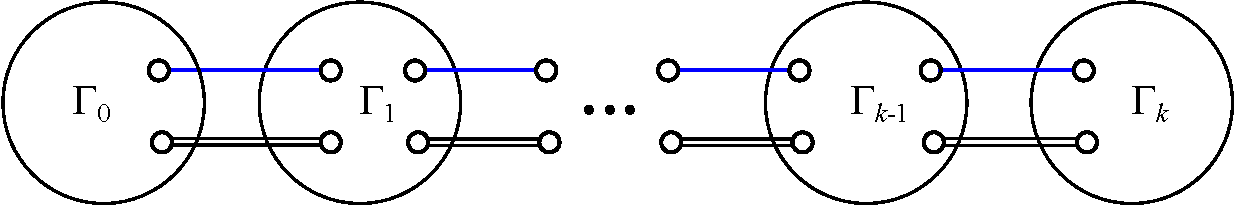
\includegraphics[width=10cm]{chain0.pdf}} 
\ee
Here we draw a molecular graph without red solid edges, and inside the black circles are some subgraphs. $\Gamma_k$ is the minimal isolated subgraph (MIS) $\Iso_k$, $\Gamma_k \cup \Gamma_{k-1}$ plus the two edges between them form the isolated subgraph $\Iso_{k-1}$, and $\Gamma_k \cup \Gamma_{k-1} \cup \cdots \cup \Gamma_{k-i}$ plus the edges between these components form the isolated subgraph $\Iso_{k-i}$. $\Gamma_0$ is a subgraph containing internal molecules that are connected with external edges, and we do not treat it as an isolated subgraph. The term ``pre-deterministic" refers to that the MIS of a SPD graph is pre-deterministic.   

As a key step of our proof, we will show that the SPD property will be preserved both in local expansions (cf. Lemma \ref{lem localgood2}) and global expansions (cf. Lemma \ref{lem globalgood}) if we always expand the \emph{first blue solid edge} in a pre-deterministic order of the MIS of every SPD graph. Hence continuing expansions, we can finally expand $T_{\fa, \fb_1\fb_2}$ into a sum of SPD graphs, which, by definition, imply the doubly property of them. However, unlike pre-deterministic graphs, a SPD graph is not always expandable.    
For example, if \eqref{deter_comps} corresponds to a locally standard atomic graph and all its components $\Gamma_i$ do not contain any blue solid edges, then the atomic graph only contains pivotal blue solid edges and cannot be expanded without breaking the doubly connected property.


\subsubsection{Globally standard property} % \hty{ I am confused which graphs are globally standard}}


Our goal is thus to find a graphical property as a compromise between the pre-deterministic and SPD properties, so that it is preserved in both local and global expansions and also guarantees that we will not get non-expandable graphs. We will identify such a property in Definition \ref{defn gs}, called the \emph{globally standard property}. Roughly speaking, a globally standard graph is a SPD graph such that its MIS is connected with at least two external red solid edges.  First, using the fact that the SPD property is preserved by local and global expansions, % and keeping track of the number of external red solid edges of isolated subgraphs, 
it is not hard to show that the globally standard property is also preserved by both local and global expansions (as long as we always expand the first blue solid edge in a pre-deterministic order of the MIS). Second, a globally standard graph is always expandable. To see why, we consider the setting \eqref{deter_comps}. If $\Gamma_k$ contains at least one blue solid edge, then it contains a redundant edge due to its pre-deterministic property. Otherwise, $\Gamma_k$ is connected with at least two external red solid edges and at most one blue solid edge. 
This shows that we cannot have a perfect pairing between blue and red solid edges, so the graph is not locally standard. Then we can apply local expansions to the graph. 

%One novel observation of this paper is that the graphs in our expansions actually satisfy a \emph{globally standard property} (cf. Definition \ref{defn gs}), which is strictly stronger than the doubly connected property. Moreover, globally standard graph has the following three key features. First, the globally standard property is also preserved by local expansions. Second, in a locally and globally standard graph, there is a canonical choice of the $T$-variable so that after replacing it with the $(n-1)$-th order $T$-expansion, the resulting graphs are still globally standard. Third, a globally standard graph can be always expanded without breaking the doubly connected property, unless it is already deterministic (except for some external edges connected with $y$ or $y'$). These graphs will give rise to the first term on the right-hand side of \eqref{T-exp-intro}. With the above three features, 

Now our expansion strategy roughly proceeds as follows. We first apply local expansions to \eqref{seconduniversal} to get locally and globally standard graphs. Then we expand the first blue solid edge in a pre-deterministic order of the MIS in every graph using 
the $(n-1)$-th order $T$-expansion. Next we apply local expansions to the resulting graphs and get some new locally and globally standard graphs. In every such graph, we further expand the first blue solid edge in a pre-deterministic order of the MIS. Repeating this process for sufficiently many times, we finally obtain a linear combination of graphs that can be written into the form \eqref{mlevelT incomplete}. Throughout the expansion process, the doubly connected property is preserved, so all the graphs in \eqref{mlevelT incomplete} are also doubly connected. 

%Moreover, all graphs are doubly connected since the globally standard property includes the doubly connected property in its definition. 




%\subsection{Main structure of the proof}  
%The  proof of Theorem \ref{main thm}  is organized as an induction in $n$, the scaling order of the $T$-expansions. 
%
%\vspace{5pt}
%
%\noindent{\bf Step 1:} We first find the second and third order $T$-expansions by 
%a direct Gaussian integration by parts calculation, which is the content of the following lemma. The details of the proof will be given in Section \ref{sec Thetaexp}, where \eqref{seconduniversal} gives the second order $T$-expansion and \eqref{thirduniversal} gives the third order $T$-expansion.
%
%\begin{lemma}\label{2nd3rd T}
%There exist second and third order $T$-expansions satisfying Definition \ref{defn genuni} with $\Sigma^{(2)}=\Sigma^{(3)}=0$.
%\end{lemma}
%
%%\vspace{5pt}
%
%\noindent{\bf Step 2:}  Assume by induction that the $k$-th order $T$-expansion is given for $2\le k \le n-1$. 
%%$k$-th order $T$-expansions for all $1\le k\le n-1$ are given. 
% %[question: do we need all $k$ or just $n-1$?] {\cob[Either will be ok. The $(n-1)$-th order $T$-expansion can be also used as lower order $T$-expansions.]} 
% We will show that Theorem \ref{main thm} holds in a restrictive range of $L$. More precisely, we claim the following result. 
%
%\begin{theorem}\label{thm ptree}
%Fix any $n\in \N$. Suppose the assumptions of Theorem \ref{main thm} hold, and we have $k$-th order $T$-expansions for $2\le k \le n-1$ as in Definition \ref{defn genuni} (together with the additional properties in Definition \ref{def genuni} and Definition \ref{def genuni2}). 
%%Suppose for all $2l\le k \le n-1$, properties \eqref{two_properties0R}-\eqref{3rd_property0R} hold for $R_{2l}^{(k)}$. 
%Assume that $L$ satisfies 
%\be\label{Lcondition0}  {L^2}/{W^2}  \le W^{(n/2-1)d-c_0} \ee
%for some constant $c_0>0$. Then for any constant $\e>0$, the estimate \eqref{locallaw} holds uniformly in all $z= E+\ii\eta$ with $E\in (-2+\kappa,2-\kappa)$ and $\eta\ge W^{2+\e}/L^2$.
%\end{theorem}
%
%
%%
%%Then we can prove the estimate \eqref{locallaw} for $L$ satisfying the constraint \eqref{Lcondition0}. This will be given in Theorem \ref{thm ptree}.
%
% 
%
%\noindent{\bf Step 3:}  Given the $k$-th order $T$-expansion for $1\le k\le n-1$, we will construct an $n$-th order \emph{incomplete} $T$-expansion  in Theorem \ref{incomplete Texp}.  
% 
%\vspace{5pt}
%
%\noindent{\bf Step 4:} Using Theorem \ref{thm ptree} and the $n$-th order {incomplete} $T$-expansion in Theorem \ref{incomplete Texp}, in Lemma \ref{cancellation property} we will prove the sum zero property for the $n$-th order $\self$ $\Sele_n$ in \eqref{decompose Sdelta}
%
%\vspace{5pt}
%
%\noindent{\bf Step 5:} Based on the $n$-th order {incomplete} $T$-expansion in Theorem \ref{incomplete Texp}, using the sum zero property proved in Step 4 we can construct an $n$-th order $T$-expansion  in Corollary \ref{lem completeTexp}.  
%
%%A key ingredient in this step 
%%is to use Theorem \ref{thm ptree}  %for $(n-1)$-th order $T$-expansion 
%%to prove  the $n$-th order sum zero property \eqref{weaz} for the self-energy term $\Sele^{\infty}_{n}$ in $\Sinfty_{n}$. A more precise statement  will be given in  Lemma \ref{cancellation property} in Section \ref{sec sumzero1}.
% 
%\vspace{5pt}
%
% Combining the above steps, by induction in $n$, we  obtain an $n$-th order $T$-expansion for any fixed $n\in \N$. Theorem \ref{thm ptree} then implies that  \eqref{locallaw} holds for $L$ satisfying \eqref{Lcondition0} for any  $n\in \N$. This proves Theorem \ref{main thm} since  $n$ is arbitrary. In Figure \ref{Fig pfchart1}, we illustrate the structure of the whole proof with a flow chart. 
%
% 
%
%\begin{figure}[htb]
%\color{black}
%\tikzstyle{startstop} = [rectangle,rounded corners, minimum width=1cm,minimum height=0.5cm,text centered, draw=black]
%\tikzstyle{startstop3} = [rectangle,rounded corners, minimum width=3cm, text width=6em, minimum height=0.5cm,text badly centered, draw=black]
%\tikzstyle{block} = [rectangle, draw=black, %fill=blue!20, 
%    text width=12em, text centered, rounded corners, minimum height=1.5em]
%\tikzstyle{line} = [draw=black, -latex']
%\tikzstyle{line0} = [draw=black]
%\tikzstyle{decision} = [diamond, draw=black, %fill=blue!20, 
%    text width=3em, text badly centered, node distance=2cm, 
%    inner sep=0pt]
%
%\tikzstyle{cloud} = [draw=black, ellipse, %fill=red!20, 
%node distance=2.5cm,
%    minimum height=2em]
%\tikzstyle{null} = [draw=none,fill=none,right]
%
%\begin{center}  
%\begin{tikzpicture}[node distance = 1.5cm, auto]
%
%    % Place nodes
%    \node [startstop] (start) {Step 1, Lemma \ref{2nd3rd T}: 2nd and 3rd order $T$-expansions};
%    \node [block, below of= start, node distance=1.5cm] (op1) {Induction hypothesis: $k$-th order $T$-expansion, $k\le n-1$};
%    %\node [decision, below of=op1] (decide1) {Check }; 
%    \node [block, below of=op1, node distance=2cm] (op2) {Step 2, Theorem \ref{thm ptree}: Proving local law \eqref{locallaw} for $L\le L_n$};
%    \node [block, right of=op2, node distance=5.5cm] (output) {Concluding Theorem \ref{main thm} when $n=n_{W,L}$}; 
%    \node [block, below of=op2, node distance=2cm] (op3) {Step 3, Theorem \ref{incomplete Texp}: Obtaining the $n$-th order {incomplete} $T$-expansion};
%    %\node [decision, below of=op3, node distance=1.5cm] (decide3) {Check }; 
%    \node [block, below of=op3, node distance=2cm] (op4) {Step 4, Lemma \ref{cancellation property}: Showing the sum zero property for $\Sele_n$ in \eqref{decompose Sdelta}};
%    %\node [decision, below of=op4, , node distance=1.5cm] (decide4) {Check }; 
%    \node [block, below of=op4, node distance=2cm] (op5) {Step 5, Corollary \ref{lem completeTexp}: Obtaining the $n$-th order $T$-expansion};
%    \node [cloud, left of=op3, node distance=5cm] (update) {Induction: $n+1 \to n$};
%
%    \path [line] (start) -- (op1);
%    \path [line] (op1) -- (op2);
%    %\path [line] (op2)--(decide2);
%    \path [line] (op2) --node [midway] {} (op3);
%    \path [line] (op2) -- (output);
%    \path [line] (op3) --node [midway] {} (op4);
%    %\path [line] (op4) -- (decide4);
%    \path [line] (op4) --node [midway] {} (op5);
%    %\path [line] (op5) -- (stopE);
%    %\node [null, left of=decide1, node distance=4.12cm] (null1) {};
%    \node [null, left of=op2, node distance=4.12cm] (null2) {};
%    \node [null, right of=op2, node distance=4.12cm] (null22) {};
%    %\node [null, left of=decide3, node distance=4.12cm] (null3) {};
%    \node [null, right of=op3, node distance=4.12cm] (null33) {};
%    \node [null, left of=op4, node distance=4.12cm] (null4) {};
%    \node [null, right of=op4, node distance=4.12cm] (null44) {};
%     
%    \path [line] (update) |- (op1);
%    \path [line] (op5) -| node [near start] {} (update);
%
%\end{tikzpicture}
%\end{center}
%\caption{The main structure of the proof. Corresponding to \eqref{Lcondition0}, we denote $L_n:=W^{1+\frac{n-2}{4}d -c_0}$ for a small constant $c_0>0$. Moreover, given an $L$ in Theorem \ref{main thm}, it is enough to perform the induction up to $n_{W,L}:= \left\lceil\frac{4}{d}\left(\log_W L  - 1 + c_0\right)\right\rceil+2$.}\label{Fig pfchart1}
%\end{figure}


%
%\subsection{Step 3: Construction of incomplete $T$-expansions}
%%{\bf Next question: 4. How to construct the $n$-th order $T$-expansion?} {\cob This is the second key ingredient.}
%In this subsection and Sections \ref{sec sumzero1}-\ref{sec expT} below, we perform Steps 3-5 of the strategy below Theorem \ref{thm ptree}. In general, it is almost impossible to define the $T$-expansions explicitly (for $n=6$, there are already more than $10^4$ many terms). Instead, we adopt a different strategy, that is, we define a programmatic way to generate the $T$-expansions by specifying the elementary expansions and some rules on the sequence of expansions. For each $n$, the $n$-th order $T$-expansion obtained in this way may not be unique 
%depending on the choices of the sequence of expansions, but the existence is much more important to us. 
%
% With a strategy of expansions described in Sections \ref{sec_basiclocal} and \ref{sec global}, we can obtain the following lemma, which gives the $n$-th order \emph{incomplete $T$-expansion} as required by Step 3. The proof of Theorem \ref{incomplete Texp} will be given in Section \ref{sec expandlvl4}.
%
%\begin{lemma}    \label{incomplete Texp}
%Fix any $n\in \N$. Suppose we have defined the $k$-th order $T$-expansions for all $2\le k \le n-1$. Then we have the following expansion of $T$-variables: %for any large constant $D>0$,  
%\be %\label{mlevelT incomplete}
%T_{xy}= |m|^2 \Theta_{xy}  + \sum_{\al} \left(\Theta \wtSdelta^{(n)} \right)_{x\al}T_{\al y}  + (\PITn)_{xy} +  (\AITn)_{xy} + (\QITn)_{xy} ,%+ \OO_\prec(W^{-D}).
%\ee
%where all the expressions on the right-hand side only depend on $n$, $m(z)$, $S$, $S^{\pm}(z)$, $\Theta(z)$ and $G(z)$, but otherwise do not depend on $W$, $L$ and $d$ directly. Here $\PITn $, $\AITn$ and $\QITn$ respectively satisfy the same properties as $\PTn $, $\ATn$ and $\QTn$ in Definition \ref{defn genuni} (including the additional properties that will be given in Definition \ref{def genuni} and Definition \ref{def genuni2}). Moreover, $\wtSdeltan$ is a sum of deterministic expressions consisting of $m(z)$, $I_N$, $S$, $S^\pm(z)$ and $\Theta(z)$ only, and it can be decomposed as 
%\be %\label{decompose Sdelta} 
%\wtSdeltan = \Sele_n + \sum_{l=4}^{n-1} \Sele_{l}
%\ee
%for a sequence of $\selfs$ $\Sele_{l}$ satisfying Definition \ref{collection elements} for $1\le l \le n-1$. Finally, $\Sele_{n}$ is a sum of $\OO(1)$ many deterministic graphs of scaling order $n$, has an infinite space limit $\Sele^{\infty}_{n}$ as $L\to \infty$, and satisfies properties \eqref{two_properties0}, \eqref{4th_property0}, \eqref{two_properties0V}, \eqref{3rd_property0 diff} and \eqref{4th_property0V} with $l=n$. 
%
%%\iffalse
%%As in \eqref{trivial conv}, we have $\Sele_l=0$ for $l\in 2\N+1$. For any $4\le l \le n$ and small constant $\e>0$, we have the following properties  
%%% \begin{itemize}
%%%\item[(i)] 
%% \be \label{two_properties incomp}
%% \Sele_{l} (x, x+a) =  \Sele_{l} (0,a), \quad   \Sele_{l} (0, a) = \Sele_{l}(0,-a), \quad \forall x,a\in \Z_L^d,
%%\ee 
%%%where we used the notation $R_\Delta^{(2n)} (x, y)\equiv (R_\Delta^{(2n)})_{xy}$; 
%%  %\item[(ii)] %From the doubly connected property, we get
%%  \be \label{4th_property incomp}
%%\left|  \Sele_{l} (0,x) \right| \le W^{-ld/2} \frac{W^{d+2} }{\langle x\rangle^{d+2-\e}}, \quad \forall x\in \Z_L^d,
%%\ee
%%%and
%% \be\label{two_propertiesV incomp}
%%\Sele^{\infty}_{l}(x, x+a) = \Sele^{\infty}_{l}(0,a), \quad  \Sele^{\infty}_{l}(0, a) =\Sele^{\infty}_{l} (0,-a), \quad \forall x,a\in \Z^d,
%%\ee 
%%\be\label{3rd_property diff}
%%\left| \Selek_{l} (0,x)-\Seleinf_{l} (0,x) \right| \le W^{-ld/2} \frac{\eta W^{d} }{\langle x\rangle^{d-\e}}, \quad \forall x\in \Z_L^d,
%%\ee
%%\be\label{4th_propertyV incomp}
%%\left| \Sele^{\infty}_{l} (0,x) \right| \le W^{-ld/2} \frac{W^{d+2} }{\langle x\rangle^{d+2-\e}}, \quad \forall x\in \Z^d,
%%\ee
%%where $\Sele^{\infty}_{l}$ is the (entrywise) infinite space limit of $\Sele_{l}$ as $L\to \infty$. Moreover, the following sum zero properties hold for any $4\le l \le n-1$:
%%\be\label{3rd_property0}
%% \Big|\sum_{x\in \Z_L^d} \Sele_{l}(0,x)\Big|   \le \frac{\eta W^{\e}}{W^{(l/2-1)d }}, %\quad \forall   W^{2+\e}/L^2 \le \eta \le 1 ,
%%\ee
%%%and
%%\begin{equation} \label{weaz}
%%\sum_x (\Sele^{\infty}_{l})(0,x)=0 .
%%\end{equation}
%%\fi
%
% \end{lemma} 
%
%\begin{remark}
%We remark that Theorem \ref{incomplete Texp} is proved using an induction argument. More precisely, before constructing the $n$-th order incomplete $T$-expansion, we have obtained the $k$-th order $T$-expansion and proved the sum zero properties \eqref{3rd_property0} and \eqref{weaz} for all $\Sele_k$ with $k\le n-1$. On the other hand, $ \Sele_n$ is a new deterministic expression obtained in the $n$-th order incomplete $T$-expansion, whose sum zero properties are yet to shown. %We also remark that the expressions $\Sele_{l}$ in Theorem \ref{incomplete Texp} satisfies the properties (i)-(iii) of Definition \ref{collection elements}, and hence we include it into the set $\Cele_{l}$.
%\end{remark}
%
% 
%We call \eqref{mlevelT incomplete} an $n$-th order {\bf incomplete} $T$-expansion, in the sense that $T_{\al y}$ in the second term on the right-hand side has not been expanded yet. If we can replace $T_{\al y}$ with a $|m|^2\Theta_{\al y}$ or a $|m|^2 (\Theta \Sdelta^{(k)}\Theta)_{\al y}$ (as in the $k$-th order $T$-expansion), then we obtain the $n$-th order (complete) $T$-expansion in \eqref{mlevelTgdefintro}. But before doing that, we need to show that $\Sele_n$ also satisfies the sum zero properties \eqref{3rd_property0} and \eqref{weaz}, which is the purpose of Step 4. The proof uses the expression \eqref{mlevelT incomplete} in a crucial way.
%
%
%%these properties \eqref{two_properties incomp}-\eqref{weaz} for $ \Sele_{2l}$, $4\le 2l \le n-1$, actually follow from the lower order incomplete $T$-expansions. So we have assumed them in Theorem \ref{incomplete Texp}. {\cob note $\Sele_k$ is an element of ...... $\Sele_k$ does not depend on $n$}
%
%
%%sum zero property.  %(recall Lemma \ref{2nd3rd T}). 
%
%%Then it is crucial to show that they also hold for $\Sele_{n} $.  
%   
%%-----old contents   
%%\begin{lemma}\label{lem Rsymm}
%%The property \eqref{two_properties incomp} holds for $\Sele_{n} $ in Theorem \ref{incomplete Texp}. 
%%\end{lemma}
%%\begin{proof}
%%This lemma is a simple consequence of the fact that all the matrices $S$, $S^{\pm}(z)$ and $\Theta(z)$ satisfy the two properties in \eqref{two_properties incomp}. Take any expression in $\Sele_{n} $, say $\Sele_{n, \gamma}$, it can be written into the general form
%%\begin{align*}
%%\Sele_{n,\gamma}(x,y)=\sum_{x_1,\cdots, x_\ell}\prod_{(x,x_i)\in \mathbf E}f_{i}(x,x_i)\cdot \prod_{(x_i,x_j)\in \mathbf E}f_{ij}(x_i,x_j) \cdot \prod_{(x_j,y)\in \mathbf E}g_{j}(x_j,y),
%%\end{align*}
%%where $\mathbf E$ is the collection of all pairs of indices of the matrix entries in $\Sele_{n,\gamma}$ (here $\mathbf E$ can be regarded as the set of edges in the graph representing $\Sele_{n,\gamma}$), and each entry $f_{i}$, $f_{ij}$ and $g_j$ satisfies the two properties in \eqref{two_properties incomp}. Then we have  
%%\begin{align*}
%%\Sele_{n,\gamma} (x , x+a) &=\sum_{x_1,\cdots, x_\ell}\prod_{(x,x_i)\in \mathbf E}f_{i}(x,x_i)\cdot \prod_{(x_i,x_j)\in\mathbf E}f_{ij}(x_i,x_j) \cdot \prod_{(x_j,y)\in\mathbf E}g_{j}(x_j,x+a) \\
%% &=\sum_{x_1,\cdots, x_\ell}\prod_{(x,x_i)\in\mathbf E}f_{i}(0,x_i-x)\cdot \prod_{(x_i,x_j)\in\mathbf E}f_{ij}(x_i-x,x_j-x) \cdot \prod_{(x_j,y)\in\mathbf E}g_{j}(x_j-x,a) \\
%% &=\sum_{x_1,\cdots, x_\ell}\prod_{(x,x_i)\in\mathbf E}f_{i}(0,x_i)\cdot \prod_{(x_i,x_j)\in\mathbf E}f_{ij}(x_i,x_j) \cdot \prod_{(x_j,y)\in\mathbf E}g_{j}(x_j,a) =\Sele_{n,\gamma} (0 , a) ,
%%\end{align*}
%%and 
%%\begin{align*}
%%\Sele_{n,\gamma} (0 , a) &=\sum_{x_1,\cdots, x_\ell}\prod_{(0,x_i)\in\mathbf E}f_{i}(x,x_i)\cdot \prod_{(x_i,x_j)\in\mathbf E}f_{ij}(x_i,x_j) \cdot \prod_{(x_j,y)\in\mathbf E}g_{j}(x_j,a) \\
%% &=\sum_{x_1,\cdots, x_\ell}\prod_{(x,x_i)\in\mathbf E}f_{i}(0,-x_i)\cdot \prod_{(x_i,x_j)\in\mathbf E}f_{ij}(-x_i,-x_j) \cdot \prod_{(x_j,y)\in\mathbf E}g_{j}(-x_j,-a) \\
%% &=\sum_{x_1,\cdots, x_\ell}\prod_{(x,x_i)\in\mathbf E}f_{i}(0,x_i)\cdot \prod_{(x_i,x_j)\in\mathbf E}f_{ij}(x_i,x_j) \cdot \prod_{(x_j,y)\in\mathbf E}g_{j}(x_j,-a) =\Sele_{n,\gamma} (0 , -a) ,
%%\end{align*}
%%where we used that for $f$ satisfying \eqref{two_properties incomp}, $f(-x,-y)=f(0,x-y)=f(0,y-x)=f(x,y).$ Hence we conclude the proof with the above two identities.
%%\end{proof}
%%
%%\begin{lemma}\label{lem Rdouble0}
%%The property \eqref{4th_property incomp} holds for $\Sele_{n} $ in Theorem \ref{incomplete Texp}. 
%%\end{lemma}
%%\begin{proof}
%%This lemma is a special case of Lemma \ref{lem Rdouble} below.
%%\end{proof}
%%------------------
% 
%
% 
%
%%\begin{remark}
%%We can prove the properties \eqref{two_properties0} and \eqref{4th_property0} for $\Sdelta_{n}$ with the same arguments as in Lemma \ref{lem Rsymm} and Lemma \ref{lem Rdouble}. On the other hand, the sum zero property \eqref{weaz} follows easily from Lemma \ref{cancellation property}, because $\Sinfty_{n}$ can be written as
%% $$\Sinfty_{n}=\sum_{2l\le n} \sum_\al  \wtSinfty_{2l} \Gamma_{n-2l+2}, $$
%% for some matrices $\Gamma_{n-2l+2}$ with summable rows and scaling orders $(n-2l+2)$. More details will be given in the proof of Lemma \ref{lem completeuni}.
%% \end{remark}
%
% \begin{lemma}\label{cancellation property}
%	Suppose we have the incomplete $n$-th order $T$-expansion in Theorem \ref{incomplete Texp}. Then the properties \eqref{3rd_property0} and \eqref{weaz} hold for $\Sele_{n}$ with $l=n$. % in \eqref{decompose Sdelta}. 
%	% we have 
%	% \be\label{weaz comp}
%	% \sum_y (\Sele^{\infty}_{n})_{xy}=0,  \quad \forall x\in \Z_L^d.
%	%\end{equation}%where $\Sele^{\infty}_{n}$ is the infinite space limit of $\Sele_{n} $ as $L\to \infty$. 
%\end{lemma}
%
%\iffalse
%\subsection{Step 4: Sum zero properties}\label{sec sumzero1} 
%This subsection is devoted to proving the following lemma. 
%%The main challenge is to prove the following sum zero property. We will prove it in Section \ref{sec sumzero1} below.
%
% 
%Now we give the three main ingredients, Lemmas \ref{lem V-R wt}, \ref{lem FT0} and \ref{lem maincancel}, for the proof of Lemma \ref{cancellation property}. First, we show that the difference between the row sums of $ \Sele_{n} $ and $ \Sele^{\infty}_{n}$ are sufficiently close to each other. The proof of Lemma \ref{lem V-R wt} will be given in Section \ref{sec infspace}. 
%
%\begin{lemma} \label{lem V-R wt}%[Informal statements of some estimates]
%Fix any $n\in \N$. Suppose we have defined the $k$-th order $T$-expansions for all $2\le k \le n-1$. Then for the incomplete $n$-th order $T$-expansion in Theorem \ref{incomplete Texp}, we also have the following estimate:
%%and \eqref{two_properties incomp}-\eqref{weaz} hold for $ \Sele_{2l}$ for all $4\le2l\le n-1$. Then we have that %for all $4\le 2l \le n$, we have that
% \be\label{property V-R wt}
% \left|\sum_{x\in \Z_L^d} ( \Sele_{n})_{xy} (m(z),f, W, L) - \sum_{x\in \Z^d} ( \Sele^{\infty}_{n})_{xy}(m(E), f, W)  \right|   \le \eta W^{-(n/2-1)d+\e},\quad \forall\   W^{2+\e}/L^2 \le \eta \le L^{-\e} ,
%\ee
%for any small constant $\e>0$.
%\end{lemma}
%
%
%
%
%By taking $L\to \infty$, the infinite space limit $\sum_x  (\Sele^{\infty}_{n})_{xy}$ depends only on $n$, $m(E)$, $f$ in Assumption \ref{var profile}, and band width $W$. Now using a standard calculation with Fourier transforms on $\Z^d$, we will show that the $W$ dependence can be pulled out as a scaling factor. The proof of Lemma \ref{lem FT0} will be given in Appendix \ref{sec FT}.
%
%
%\begin{lemma}\label{lem FT0}
%Fix any $n\in \N$. For the incomplete $n$-th order $T$-expansion in Theorem \ref{incomplete Texp}, %Suppose we have defined the $k$-th order $T$-expansions for all $2\le k \le n-1$, and \eqref{two_properties incomp}-\eqref{weaz} hold for $ \Sele_{2l}$ for all $4\le2l\le n-1$. Then 
%we have that %for any $y\in \Z^d$,
%\be\label{eq FT0} W^{(n/2-1)d}\sum_{x\in \Z^d}( \Sele^{\infty}_{n})_{xy}(m(E), f, W) = {\Sint}_{n}(m(E), f) ,\ee
%where ${\Sint}_{n}$ is a constant that does not depend on $W$. %depends on $n$, $m(E)$ and $f$, but 
%\end{lemma}
%
%Finally, we show that the row sum $\sum_{x} ( \Sele_n)_{xy}(m(z),f, W, L)$ is much smaller than $W^{-(n/2-1)d}$ under certain choices of $L$ and $z$. Recall that as shown in \eqref{sum S2l}, $W^{-(n/2-1)d}$ is the bound on the $\ell^1$-norms of the rows of $\Sele_n$.
%%Then we have the following bound on a special band matrix with carefully chosen linear size $L_n$.
%
%\begin{lemma}\label{lem maincancel}
%Fix any $n\ge 3$. Suppose we have defined the $k$-th order $T$-expansions for all $2\le k \le n-1$. Suppose we have the incomplete $n$-th order $T$-expansion in Theorem \ref{incomplete Texp}. Let $L\equiv L_n$ satisfy
%\be\label{Lcondition} W^{(n/2-3/2)d+c_0} \le {L_n^2}/{W^2}  \le W^{(n/2-1)d-c_0} \ee
%for a constant $c_0>0$, and $\eta\equiv \eta_n=W^{2+\e}/L_n^2$ for a small enough constant $\e>0$. Then we have that for $z_n:= E+\ii \eta_n$, %and any $y\in \Z_L^d$,
%\be\label{small SnE0}
%\begin{split}
%\left| \sum_{x} (\Sele_n)_{xy} (m(z_n),f, W, L_n) \right|\le W^{-c} W^{-(n/2-1)d} 
%\end{split}
%\ee
%for a constant $c>0$ depending on $c_0$.
%\end{lemma}
%
%%In particular, in the proof Lemma \ref{cancellation property}, we can apply Lemma \ref{lem maincancel} with the choice 
%Note that 
%%\be\label{choice Ln}
%$ L_{n}= W^{1+\left(n/4-5/8\right)d}$
%%\ee
%is a particular choice that satisfies the condition \eqref{Lcondition} with $c_0=d/4$. Before proving Lemma \ref{lem maincancel}, we first combine it with Lemma \ref{lem V-R wt} and Lemma \ref{lem FT0} to conclude Lemma \ref{cancellation property}.
%
%\begin{proof}[Proof of Lemma \ref{cancellation property}] 
% Applying Lemma \ref{lem V-R wt} and Lemma \ref{lem FT0} with $L=L_n$ and $z=z_n$ as in Lemma \ref{lem maincancel}, we obtain that 
%\be\label{lower Sdelta} 
%  \left|\sum_{x} (\Sele_n)_{xy} (m(z_n),f, W, L_n) \right| \ge W^{-(n/2-1)d}\left|{\Sint}_{n}(m(E), f)\right| - \eta_n W^{-(n/2-1)d+\e}.
%\ee
%Combining \eqref{small SnE0} and \eqref{lower Sdelta}, we obtain that 
%%$$W^{-(n/2-1)d}\left|{\Sint}_{n}(m(E), f)\right| - \eta_n W^{-(n/2-1)d+\e} \le W^{-c} W^{-(n/2-1)d} ,$$
%%which implies that 
%$$ \left|{\Sint}_{n}(m(E), f)\right| \le \eta_n W^{\e} + W^{-c} =\oo(1).$$
%Since ${\Sint}_{n}$ is a constant, we must have ${\Sint}_{n}(m(E), f)=0$, which further implies \eqref{weaz} for $\Seleinf_n $ by Lemma \ref{lem FT0}. Then combining \eqref{weaz} for $\Seleinf_n $ with Lemma \ref{lem V-R wt}, we obtain \eqref{3rd_property0} for $\Sele_n $.
%\end{proof}
%
%For the proof of Lemma \ref{lem maincancel}, we need to use the following lemma. Its proof will be given in Section \ref{sec bound double}. The proof is based on some additional properties of $\PITn$ and $\AITn$ that will be introduced in Definition \ref{def genuni} below (more precisely, their \emph{doubly connected} properties that will be defined in Definition \ref{def 2net}).
%
%%As a consequence of the unstated properties of the expressions on the right-hand side of \eqref{mlevelTgdefintro}, we can obtain that following estimates. The proofs of these estimates will be given in Section \ref{sec Sdelta}, where we will discuss the special property---the doubly connected structure---that is behind all these proofs. 
%
%\begin{lemma} \label{lem informal}%[Informal statements of some estimates]
% %Suppose the assumptions of Lemma \ref{lem maincancel} hold. 
% %For any fixed $n\in \N$, suppose \eqref{two_properties0}-\eqref{weaz} hold for $\Sdelta_{2l}$ and $\Sele_{2l}$ for all $2l\le n-1$. 
% %Then the following estimates hold:%Roughly speaking, $(\cal E_n)_{xy}$ satisfies that 
% Fix any $n\in \N$, and take $z=z_n$, $\eta=\eta_n$ and $L\equiv L_n$ as in Lemma \ref{lem maincancel}. For the incomplete $n$-th order $T$-expansion in Theorem \ref{incomplete Texp}, we also have the following estimates:
%\be\label{intro_recol}
%\left|\sum_{x,y} (\PITk)_{xy}(z_n,f, W, L_n)\right| \prec N_n\frac{W^{-(k/2-1)d}}{\eta_n},\quad 3\le k \le n,
% \ee
%and
%\be\label{intro_error}
%%|(\ATn)_{xy}| \prec W^{-(n+1)d/2+\e},\quad 
%\left|\sum_{x,y} (\AITn)_{xy}(z_n,f, W, L_n)\right| \prec N_n\frac{W^{-(n/2-1/2)d}}{\eta_n^2},
%\ee
%where $N_n:=(L_n+1)^d$ is the number of vertices in $\Z_{L_n}^d$.
%\end{lemma}
%%The proof of this lemma will be given at the end of Section \ref{sec bound double}.
%%\begin{remark}\label{remark_upper}
%%Recall that in the setting of Lemma \ref{lem maincancel}, we have the $(n-1)$-th order $T$-expansion. Then by Theorem \ref{thm ptree}, the estimate \eqref{locallaw} holds for $G(z_n, f, W, L_n)$ if $L_n$ satisfies
%%$${L_n^2}/{W^2}  \le W^{(n/2-1)d-c_0} $$
%%This explains the upper bound in \eqref{Lcondition}. The local law \eqref{locallaw} for $G(z_n, f, W, L_n)$ will be used in the proof of \eqref{intro_recol} and \eqref{intro_error}. 
%%\end{remark}
%
% 
%
%%
%%To prove this claim, we will need the following version of Theorem \ref{main thm}, which is stated for random band matrices with system sizes satisfying the upper bound in \eqref{Lcondition1}. Its proof is based on the $(n-1)$-th order $T$-expansion together with a high moment bound on $T_{xy}$, which will be given in Section \ref{sec ptree}.
%%
%%\begin{theorem}\label{thm ptree1}
%%Suppose for all $2l\le k \le n-1$, properties \eqref{two_properties0R}-\eqref{3rd_property0R} hold for $R_{2l}^{(k)}$. Assume that $L$ satisfies 
%%\be\label{Lcondition2}  {L^2}/{W^2}  \le W^{(n/2-1)d-c_0} \ee
%%for some constant $c_0>0$. Then for any constant $\e>0$, the estimate \eqref{locallaw} holds uniformly for all $z= E+\ii\eta$ with $\eta\ge W^{2+\e}/L^2$.
%%\end{theorem}
%%Next we prove Claim \ref{claim maincancel} based on Theorem \ref{thm ptree} and the $n$-th order incomplete $T$-expansion in Definition \ref{mlevelT}.
%
%%For the proof of Lemma \ref{lem maincancel}, 
%We also record the following classical Ward's identity.
%\begin{lemma}[Ward's identity]\label{lem ward}
%For any $y,y'\in \Z_L^d$ and $z=E+\ii \eta$, we have 
%\be\label{eq_Ward0}
% \sum_x \overline G_{xy'}( z) G_{xy}( z) = \frac{G_{y'y}(z)-G_{y'y}(\overline z)}{2\ii \eta}.
% \ee
% As a special case, if $y=y'$, then
% \be\label{eq_Ward}
% \sum_x |G_{xy}( z)|^2 = \frac{\im G_{yy}(z) }{ \eta}.
% \ee
%\end{lemma}  
%\begin{proof}
%The proof of \eqref{eq_Ward0} is a simple application of the spectral decomposition of $G(z)$.  
%\end{proof}
%
%Now we are ready to give the proof of Lemma \ref{lem maincancel}.
%\begin{proof}[Proof of Lemma \ref{lem maincancel}]
%In the setting of Lemma \ref{lem maincancel}, we have the $(n-1)$-th order $T$-expansion. Then by Theorem \ref{thm ptree}, the estimate \eqref{locallaw} holds for $G(z_n, f, W, L_n)$ if $L_n$ satisfies
%$${L_n^2}/{W^2}  \le W^{(n/2-1)d-c_0} $$
%This explains the upper bound in \eqref{Lcondition}. %In the following proof, we will use the local law \eqref{locallaw} for $G(z_n, f, W, L_n)$. %will be used in the proof of \eqref{intro_recol} and \eqref{intro_error}. 
%%With \eqref{locallaw} for $G(z_n, f, W, L_n)$, we can conclude the proof: for \eqref{intro_recol}, we refer the reader to \eqref{Rcancel4}, and for \eqref{intro_error}, we refer the reader to \eqref{Rcancel5}. %[{\cor modify the references to the results below}]
%
% Taking the expectation of both sides of \eqref{mlevelT incomplete} and summing over $x,y \in \Z_L^d$, we obtain that:
%\begin{align}
%\sum_{x,y}\E T_{xy}(z_n,f, W, L_n)&= |m|^2 \sum_{x,y}\Theta_{xy}(m(z_n),f, W, L_n)  + \left[\sum_{x,\al} \left(\Theta \wtSdelta^{(n)} \right)_{x\al} \sum_{y}\E T_{\al y}\right](z_n,f, W, L_n)  \nonumber\\
%&+ \sum_{x,y}\E(\PITn)_{xy}(z_n,f, W, L_n) +  \sum_{x,y}\E(\AITn)_{xy}(z_n,f, W, L_n)  ,\label{mlevelT sum}
%\end{align}
%where we used that $\E(\QITn)_{xy} =0$. For simplicity of notations, in the following derivation we shall omit the arguments $z_n,f, W, L_n$.
%
%%Apply the $n$-th order $T$-expansion \eqref{mlevelT} to the $T$-variable $T_{\fa\fb}$, we get 
%%\be\label{after1-5n}
%% T_{\fa\fb}= m \Theta_{\fa \fb} \overline G_{\fb\fb} + \sum_x \left(\Theta \wt S^{(n)}_ \Delta \right)_{\fa x}|G_{x\fb}|^2   + (\PITn)_{\fa,\fb} +  (\AIT^{(n)}_{ho})_{\fa,\fb} + (\wt{\cal G}_{Q}^{(n)})_{\fa,\fb} + \OO_\prec(L^{-D}).
%%\ee
%For the left-hand side of \eqref{mlevelT sum}, using Ward's identity \eqref{eq_Ward} we get that 
%\begin{align}\label{Rcancel10}
%&\sum_{x,y} \mathbb E T_{xy} = |m|^2 \sum_{x, \al}s_{x\al}\left( \mathbb E \sum_y|G_{\al y}|^2\right)= |m|^2 \frac{ \sum_{x} \mathbb E\im G_{xx}}{\eta_n} =N_n |m|^2 \frac{  \mathbb E\im G_{xx}}{\eta_n},   
%\end{align}
%where we used $\mathbb E\im G_{xx}= \mathbb E\im G_{yy}$ for any $x,y\in \Z_{L_n}^d$ by symmetry. 
%For the first term on the right-hand side of \eqref{mlevelT sum}, using the identity in \eqref{sumTheta} we obtain that 
%%On the other hand, for the right-hand side of \eqref{after1-5n} we calculate the sum and expectation over each term. First, it is trivial to have $\E  (\wt{\cal G}_{Q}^{(n)})_{\fa,\fb}=0$. Using the definition of $\Theta$ in 
%%\eqref{Thetapm}, we get
%\begin{align}\label{Rcancel20}
% |m|^2 \sum_{x,y}\Theta_{xy}  = N_n\frac{|m|^4}{1-|m|^2} .
%\end{align}
%For the third term on the right-hand side of \eqref{mlevelT sum}, using \eqref{intro_recol} we obtain that for any constant $\e>0$,  
%\begin{align}\label{Rcancel30} 
%\left|\sum_{x,y}\E(\PITn)_{xy}\right| \le N_n \frac{W^{-d/2+\e}}{\eta_n},
%\end{align}
%where we also used that the lowest order graph in $\PITn$ has scaling order $\ge 3$. For the fourth term on the right-hand side of \eqref{mlevelT sum}, using \eqref{intro_error} we obtain that for any constant $\e>0$,  
%\begin{align}\label{Rcancel40} 
%\left|  \sum_{x,y}\E(\AITn)_{xy}\right| \le N_n\frac{W^{-(n/2-1/2)d+\e}}{\eta_n^2}.
%\end{align}
%Finally, for the second term on the right-hand side of \eqref{mlevelT sum}, we decompose $\wtSdeltan$ as in \eqref{decompose Sdelta}. For $4\le l \le n$, using \eqref{sumTheta} and Ward's identity we can calculate that  
%\begin{align}\label{Rcancel21}
%\sum_{x,\al} \left(\Theta \Sele_{l} \right)_{x\al} \sum_{y}\E T_{\al y} &=\frac{|m|^4}{1-|m|^2}   \sum_{w} \left( \Sele_{l}\right)_{w\al} \frac{ \sum_{x} \mathbb E\im G_{xx}}{\eta_n} = N_n \frac{|m|^4\cdot \mathbb E\im G_{xx}}{(1-|m|^2)\eta_n}\sum_{x} \left(\Sele_{l}\right)_{xy} .
%\end{align}
%By \eqref{3rd_property0} for $\Sele_l$ with $l\le n-1$, we have that 
%$$\sum_{x\in \Z_L^d}  (\Sele_{l})_{xy} \le \eta_n W^{-(l/2-1)d+\e},\quad 4\le l \le n-1.$$
%Inserting it into \eqref{Rcancel21} and using $(1-|m|^2)\sim \eta_n$, we obtain that for $4\le l \le n-1$,
%\begin{align}\label{Rcancel22}
%\left|\sum_{x,\al} \left(\Theta  \Sele_{l} \right)_{x\al} \sum_{y}\E T_{\al y}\right| \lesssim N_n \frac{W^{-(l/2-1)d+\e} \mathbb E\im G_{xx}}{\eta_n} .
%\end{align}
%
%Now plugging \eqref{Rcancel10}-\eqref{Rcancel22} into \eqref{mlevelT sum} and cancelling the $N_n$ factor on both sides, we obtain that
%%Finally combining all the estimates \eqref{Rcancel1}, \eqref{Rcancel2}, \eqref{Rcancel3}, \eqref{Rcancel4} and \eqref{Rcancel5}, we obtain from \eqref{after1-5n} that
%\begin{align}
%  |m|^2 \frac{ \mathbb E\im G_{xx}}{\eta_n} &=  \frac{|m|^4}{1-|m|^2}  +  \frac{|m|^4\cdot \mathbb E\im G_{xx}}{(1-|m|^2)\eta_n}\sum_{x} \left(\Sele_{n} \right)_{xy} \label{Rcancelsum0}\\
%&+   \OO \left(  \frac{W^{-d/2+\e}}{\eta_n}+\frac{W^{-(n/2-1/2)d+\e}}{\eta_n^2} +\sum_{4\le l \le n-1} \frac{W^{-(l/2-1)d+\e} \mathbb E\im G_{xx}}{\eta_n}\right) .\nonumber
%\end{align}
%Since \eqref{locallaw} holds for $G(z_n, f, W, L_n)$, we have 
%\be\label{insert Gxx}\E G_{xx}=m+\OO(W^{-d/2+\e}).\ee 
%Moreover, taking the imaginary part of the equation $z=-m-m^{-1}$, we obtain the equality 
%\be\label{insert m^2}\frac{|m|^2}{1-|m|^2}  = \frac{ \im m}{\eta_n} .\ee
%Inserting \eqref{insert Gxx} and \eqref{insert m^2} into \eqref{Rcancelsum0} and using $(1-|m|^2)\sim \eta_n$, we get that
%$$\left|\sum_{x} (\Sele_{n} )_{xy} (m(z_n),f, W, L_n) \right|\le   W^{-d/2+\e}\eta_n + W^{-(n-1)d/2+e} = W^{-d/2+\e}\frac{W^{2+\e}}{L_n^2} + W^{-(n/2-1/2)d+\e}.$$
%Together with the lower bound in condition \eqref{Lcondition}, we can conclude \eqref{small SnE0} for $c= \min(d/2-\e, c_0-2\e)$. 
% \end{proof}
% 
%
%
%%Recall the above evolution of this $T$-expansion  from $D^{(m\le n)}$ to $D^{(n+1)}$. One can (only) run this process   for a band matrix whose size is $(L\le L_n, W)$. 
%%
%%Hence we can obtain an expansion on $ T$  for $(L=L_n$, $W$, $\eta=W^2/L_n^2)$ with $m$-th ($m\le n$)  $T$-expansion and obtain 
%% 
%%$$
%%T\sim O(\Theta)+\Theta \cal D^{(n+1)}\Theta+  \cal Q^{(n+1)}+ O(W^{-n+1}+\frac{1}{W^2L_n^{d-2}})
%%$$
%%but up to here, we have not proved that  $\cal D^{(n+1)}$ has sum zero property. 
%% 
%% 
%% Then with above expansion, we sum up indices and take expectation, of both sides, then  in case $\eta=W^2/L^2$, we have
%%$$
%%\mathbb E \sum_{y} T_{xy}\sim   \eta^{-1} +  \eta^{-2}O(\sum_y D_{xy}^{(n+1)}),\quad \eta=W^2/L^2
%%$$
%%With Ward's identity, the left side has the order of $\eta^{-1}$. Hence we have \eqref{weaz}. 
%%{\cob My argument maybe not quite correct, please fix the details. }.  
%
%\fi
%
%\subsection{Step 5 and Proof of Theorem \ref{main thm}}\label{sec expT}
%
%After proving the sum zero properties \eqref{3rd_property0} and \eqref{weaz} for $ \Sele_{n} $, we can further expand the $T_{\al y}$ in the second term on the right-hand side of  \eqref{mlevelT incomplete} to obtain the $n$-th order (complete) $T$-expansion. %The proof of the following lemma will be given in Section \ref{sec global}.
% The proof of the following lemma will be given in Section \ref{sec lastglobal}.
% \begin{lemma}\label{lem completeTexp}
%Fix any $n\in \N$. Suppose we have defined the $k$-th order $T$-expansions for all $2\le k \le n-1$. Suppose we have the $n$-th order incomplete $T$-expansion in Theorem \ref{incomplete Texp}, such that $\Sele_n $ satisfies \eqref{3rd_property0} and \eqref{weaz}. Then 
%%there exists a sequence of sets $\Cele_{2k}$ satisfying Definition \ref{collection elements} for $2\le 2k \le n-1$, such that 
%we can obtain an $n$-th order $T$-expansion as in Definition \ref{defn genuni}.
%\end{lemma}
%
% 
% \begin{remark}
%The reason why we need to obtain an incomplete $T$-expansion before the complete $T$-expansion is as follows. If we expand the $T_{\al y}$ in the second term on the right-hand side of  \eqref{mlevelT incomplete} without knowing the sum zero properties \eqref{3rd_property0} and \eqref{weaz} for $\Sele_n $, then the higher order graphs in $(\ATn)_{xy}$ will not satisfy the desired properties and cannot be bounded in the correct way.  More details will be discussed in Remark \ref{remark bad}.
%\end{remark}
%
%\iffalse
%
%Finally, we gather all the ingredients into the proof of Theorem \ref{main thm}.
%\begin{proof}[Proof of Theorem \ref{main thm}]
%As illustrated in Figure \ref{Fig pfchart1}, we prove Theorem \ref{main thm} using an induction argument on the order of the $T$-expansions. 
%
%\medskip
%\noindent{\bf Step 1:} By Lemma \ref{2nd3rd T}, we can define the second and third order $T$-expansions. 
%
%\medskip
%\noindent{\bf Step 2:} Suppose we have defined the $k$-th order $T$-expansions for all $2\le k \le n-1$. Then applying Theorem \ref{thm ptree}, we obtain that the local law \eqref{locallaw} holds as long as long $L\le L_n:=W^{1+\frac{n-2}{4}d -c_0}$ for a constant $c_0>0$.
%
%\medskip
%\noindent{\bf Step 3:} With the $k$-th order $T$-expansions for $2\le k \le n-1$, we can construct an $n$-th order incomplete $T$-expansion as in  Theorem \ref{incomplete Texp}. 
%
%\medskip
%\noindent{\bf Step 4:} Using the local law \eqref{locallaw} in Step 2 and the $n$-th order incomplete $T$-expansion in Step 3, we can obtain the sum zero properties \eqref{3rd_property0} and \eqref{weaz} for $\Sele_n$ in \eqref{decompose Sdelta} using Lemma \ref{cancellation property}. 
%
%%we get an expansion as in \eqref{mlevelT incomplete}. By Lemmas \ref{lem Rsymm}-\ref{cancellation property}, we know that properties \eqref{two_properties incomp}-\eqref{weaz} hold for $\wtSdelta_n$. 
%
%%In particular, in the proof Lemma \ref{cancellation property}, we can apply Lemma \ref{lem maincancel} with the choice 
%%\be\label{choice Ln}
%% L_{n}= W^{1+\left(n/4-5/8\right)d},
%%\ee
%%which satisfies the condition \eqref{Lcondition} with $c_0=d/4$. 
%
%\medskip
%\noindent{\bf Step 5:}  With the $n$-th order incomplete $T$-expansion in Step 3 and the sum zero properties for $\Sele_n$ in Step 4, applying Corollary \ref{lem completeTexp} we can obtain an $n$-th order $T$-expansion. 
%
%\medskip 
%After obtaining the $n$-th order $T$-expansion, we can repeat Steps 2-5 to obtain the $(n+1)$-th order $T$-expansions, and so on. Perform the induction until we have constructed the $k$-th order $T$-expansions for all $2\le k \le n_{W,L}$, with $n_{W,L}:= \left\lceil\frac{4}{d}\left(\log_W L  - 1 + c_0\right)\right\rceil+2$. Then applying Theorem \ref{thm ptree}, we can conclude Theorem \ref{main thm}. 
%%\be\label{WL highmoment} \log_W L \le 1 + \frac{n-1}{4}d - c_0 ,\ee
%%which is obtained from the condition \eqref{Lcondition0}. Then applying Theorem \ref{thm ptree}, we can conclude the proof.
%%By Theorem \ref{thm ptree}, in order to conclude Theorem \ref{main thm}, we need to find an $n$-th order $T$-expansion such that for some constant $c_0$,
%%\be\label{WL highmoment} \log_W L \le 1 + \frac{n-1}{4}d - c_0 ,\ee
%%which is obtained from the condition \eqref{Lcondition0}.
%\end{proof}
%The rest of this paper is devoted to proving the lemmas used in the above proof of Theorem \ref{main thm}. For the reader's convenience, we summarize the lemmas left to be proved, and where one can find their proofs.
%\begin{itemize}
%
%\item Lemma \ref{2nd3rd T} will be proved in Section \ref{sec Thetaexp}.
%
%\item Lemma \ref{lem: ini bound} will be proved in Section \ref{sec ini_bound}.
%
%\item Lemma \ref{eta1case0} and Lemma \ref{lemma ptree} will be proved in Section \ref{sec ptree}.
%
%\item The proof of Theorem \ref{incomplete Texp} is the main goal of Sections \ref{sec_basiclocal} and \ref{sec global}, and in Section \ref{sec expandlvl4} we will give the final proof that collects all pieces altogether.
%
%\item Lemma \ref{lem V-R wt} will be proved at the end of Section \ref{sec infspace}.
%
%\item Lemma \ref{lem informal} will be proved at the end of Section \ref{sec bound double}.
% 
%\item Corollary \ref{lem completeTexp} will be proved in Section \ref{sec lastglobal}.
%
%\item  %will be proved in Appendix \ref{sec Qterm}, and 
%Lemma \ref{lem FT0} will be proved in Appendix \ref{sec FT}. This proof is relatively independent of the other ones. 
% 
%%\item For the interested reader, the estimate \eqref{intro_redagain} will be proved in Section \ref{sec double} (although \eqref{intro_redagain} was not used explicitly in the above proof of Theorem \ref{main thm}). 
%\end{itemize}
%Before giving the formal proofs of these lemmas, in Section \ref{sec strategy} we describe some important new ideas developed for our purpose. %We remark that some of these ideas have not been used in previous literature as far as we are concerned.
%
%\fi






\section{Basic graph operations}\label{sec_basiclocal}
  
A graph operation $\cal O[\cal G]$ on a graph $\cal G$ is a linear combination of new graphs such that the graph value of  $\cal G$ 
is \emph{unchanged}, i.e. $\llbracket \cal O[\cal G]\rrbracket=\llbracket \cal G\rrbracket$. All graph operations are linear, that is,
\be\label{linear graphO} \cal O\Big[\sum_i c_i  \cal G_i\Big] =\sum_i c_i \cal O\left[ \cal G_i\right].
\ee
The graphs operations in Sections \ref{sec_dotted}--\ref{subsec global} have been defined in \cite[Section 3]{PartI_high}, while the $Q$-expansions in Section \ref{sec defnQ} are new. 
  
\subsection{Dotted edges operations}\label{sec_dotted}
  
  

%We always identify pairs of internal atoms that are connected through dotted edges, but we will {\bf never} identify a pair of external and internal atoms, because they play very different roles. Dotted edges between internal atoms may appear in some middle steps, so we define the following merging operation. 
%  \begin{definition}[Merging operation]\label{def merge}
%  	Given a graph $\cal G$ that contains dotted edges between different atoms, we define an operator $\cal O_{merge}$ in the following way: $\cal O_{merge}[\cal G]$ is a graph obtained by merging every pair of internal atoms, say $\al$ and $\beta$, that are connected by a path of dotted edge into a single internal atom, say $\gamma$. Moreover, the weights and edges attached to $\al$ and $\beta$ in $\cal G$ are now attached to atom $\gamma$ in $\cal O_{merge}[\cal G]$. In particular, the $G$ edges between $\al$ and $\beta$ become weights on $\gamma$, and the waved and $\dashed$ edges between $\al$ and $\beta$ become self-loops on $\gamma$. 
%  \end{definition}
%  \begin{remark}
%  	It is easy to see that the graph operator $\cal O_{merge}$ is an identity in the sense of graph values:
%  	$$ \llbracket \cal O_{merge}[\cal G]\rrbracket=\llbracket \cal G\rrbracket.$$
%  	Moreover, we remark that a path of dotted edges can pass through an external atom, but we will not identify the internal atom on this path with the external atom.  
%  \end{remark}
%  
%  Given any regular graph, say $\cal G$, it is easy to write it as a linear combination of normal regular graphs using the following \emph{dotted edge partition} operation. This operation and the merging operation are the two most basic graph operations.   Later in Section \ref{sec_basiclocal}, we will introduce more advanced graph operators that expand one graph into the linear combination of several new graphs, while keeping the graph values unchanged. 
  
  %\iffalse
  %More precisely, if $\cal G$ does not satisfy the {off-$G$-property}, then we first assign the following {\bf dotted-line partition} of all the pairs of atoms that are connected by a $G$ edge. In other words, given two atoms $\al$ and $\beta$, if there are $G$ edges between them, then we decompose 
  %\be\label{assigndot}1= \mathbf 1_{\al\ne \beta} + \mathbf 1_{\al = \beta}. \ee
  %If there is a $\times$-dotted line between $\al$ and $\beta$, then the edges between them are all off-diagonal; otherwise, all the edges become weights on $\al$ or $\beta$. In this way, we can write %a graph $\cal G$ as 
  %$$\left\llbracket \cal G \right\rrbracket= \sum \left\llbracket \cal O_{merge}[{Dot} \cdot \cal G ]\right\rrbracket,$$
  %where each ${Dot}$ is a product of some dotted and $\times$-dotted edges such that each ${Dot} \cdot \cal G$ satisfies the {off-$G$-property}. Here the sum is over all possible self-consistent ${Dot}$, where the {\bf self-consistency} means: if $x_i$ and $x_j$ are connected by a dotted edge in ${Dot}$, and $x_j$ and $x_l$ are also connected by a dotted edge in ${Dot}$, then $x_i$ and $x_l$ {\bf cannot} be connected by a $\times$-dotted edge in ${Dot}$. The operator $\cal O_{merge}$ merges all pairs of internal atoms in ${Dot} \cdot \cal G$ connected by a dotted edge.
  %  \fi
  
  %We first give two graph operators related to the dotted and $\times$-dotted edges in the graphs. 
%  \begin{definition}[Dotted edge partition] \label{dot-def}%  \cob (need details, the notations can be changed to anything you like) \nc 
%  	%{\bf Assigning dotted-line partition $\cal O_{dot}$:} 
%  	Given a regular graph $\cal G$, for any pair of atoms $\al$ and $\beta$, if there are $G$ edges but no $\times$-dotted edge between them, then we write 
%  	$$1= \mathbf 1_{\al\ne \beta} + \mathbf 1_{\al = \beta};$$
%  	if there is a $\times$-dotted line $ \mathbf 1_{\al\ne \beta}$ and but  no $G$ edge between them, then we write 
%  	$$\mathbf 1_{\al\ne \beta} =1 - \mathbf 1_{\al = \beta}.$$
%  	Expanding the product of all these sums on the right-hand sides, we can write $\cal G$ as
%  	\be\label{odot}\cal O_{dot}[\cal G]= \sum \cal O_{merge}[{\Dot} \cdot \cal G],\ee
%  	where each ${\Dot}$ is a product of dotted and $\times$-dotted edges together with a $+$ or $-$ sign. %such that $\cal O_{merge}[{\Dot} \cdot \cal G]$ is a normal regular graph.
%  	In ${\Dot} \cdot \cal G$, if there is a $\times$-dotted line between $\al$ and $\beta$, then the $G$ edges between them are off-diagonal; otherwise, the $G$ edges between them become weights after the merging operation. Here we only sum over ${\Dot}$'s that are {\bf self-consistent}, that is, if $x_i$ and $x_j$ are connected by a dotted edge in ${\Dot}$, and $x_j$ and $x_k$ are connected by a dotted edge in ${\Dot}$, then $x_i$ and $x_k$  cannot be connected by a $\times$-dotted edge in ${\Dot}$. (Note if $\Dot$ is not self-consistent, then $\llbracket \Dot \cdot \cal G\rrbracket=0$.) Finally, if the graph $\cal G$ is already normal, then $\cal O_{dot}$ acting on $\cal G$ is a null operation and we let $\cal O_{dot}[\cal G]:=\cal G$.
%  	
%  	In general, for a linear combination of graphs  $\sum_i c_i \cal G_i$, where $\{c_i\}$ is a sequence of coefficients and $\cal G_i$ is a sequence of graphs, we define
%  	$$ \cal O_{dot}\left[\sum_i c_i  \cal G_i\right]:=\sum_i c_i \cal O_{dot}\left[ \cal G_i\right].$$
%  	
%  	% \medskip
%  	%\noindent  {\bf Removing $\times$-dotted lines $\cal O_{rDot}$:} 
%  	%  Given a regular graph $\cal G$, for any pair of atoms $\al$ and $\beta$, if there is a $\times$-dotted line $ \mathbf 1_{\al\ne \beta}$ and but {\bf no} $G$ edge between them, then we write 
%  	% $$\mathbf 1_{\al\ne \beta} =1 - \mathbf 1_{\al = \beta}.$$
%  	% Expanding the product of all these sums, we can expand $\cal G$ as
%  	% \be\label{ordot}\cal O_{rDot}(\cal G)= \sum \cal O_{merge}[\rDot \cdot \cal G],\ee
%  	% where each ${\rDot}$ is a self-consistent product of dotted and $\times$-dotted edges together with a $+$ or $-$ sign. Each ${\rDot} \cdot \cal G$ satisfies the following {\bf reverse off-$G$-property}: for any pair of atoms in the graph, there is a $\times$-dotted edge between them {\bf only if} there is at least one $G$ edge between them (in other words, if there is no $G$ edge between this pair of atoms, then they are not connected by $\times$-dotted edge). Finally, if the graph $\cal G$ already satisfies the reverse off-$G$-property, then $\cal O_{rDot}$ acting on $\cal G$ is a null operation and we let $\cal O_{rDot}[\cal G]:=\cal G$.
%  	
%  	
%  	
%  	%  Suppose the graph $\cal G=\mathbf 1_{\al\ne \beta} f(G)$ contains a $\times$-dotted line $ \mathbf 1_{\al\ne \beta}$ and there is no $G$ edge between $\al,\beta$. Then we expand it as
%  	% \be\label{ordot}\cal O_{rDot}(\al,\beta) \left[\mathbf 1_{\al\ne \beta} f(G)\right]= f(G) - \mathbf 1_{\al=\beta} f(G) .\ee
%  	%\end{description}
%  \end{definition}


Recall that a dotted edge between atoms $\al$ and $\beta$ represents a $\delta_{\al\beta}$ factor. We will identify internal atoms  connected by dotted edges, but we will {\it not} identify an external and an internal atom due to their different roles in graphs. We define the following simple merging operation regarding dotted edges. 
\begin{definition}[Merging operation]\label{def merge}
	Given a graph $\cal G$ that contains dotted edges between different atoms, we define an operator $\cal O_{merge}$ in the following way: $\cal O_{merge}[\cal G]$ is a graph obtained by merging every pair of internal atoms, say $\al$ and $\beta$, that are connected by a path of dotted edges into a single internal atom, say $\gamma$. Moreover, the weights and edges attached to $\al$ and $\beta$ %in $\cal G$ 
	are now attached to the atom $\gamma$ 
	in $\cal O_{merge}[\cal G]$. In particular, the $G$ edges between $\al$ and $\beta$ become weights on $\gamma$, and the waved and $\dashed$ edges between $\al$ and $\beta$ become self-loops on $\gamma$. 
\end{definition}
%\begin{remark}
%It is easy to see that the graph operator $\cal O_{merge}$ is an identity in the sense of graph values:
%$ \llbracket \cal O_{merge}[\cal G]\rrbracket=\llbracket \cal G\rrbracket$.
%We  stress  that a path of dotted edges can pass through an external atom, but we will not identify the internal atoms on this path with the external atom.  \hty{We  stress  that  we will not identify  internal atoms which are connected by dotted edges only through an external atom.}
%\end{remark}
Given any regular graph, we can rewrite it into a linear combination of normal regular graphs using the following \emph{dotted edge partition} operation. 

%\iffalse
%More precisely, if $\cal G$ does not satisfy the {off-$G$-property}, then we first assign the following {\bf dotted-line partition} of all the pairs of atoms that are connected by a $G$ edge. In other words, given two atoms $\al$ and $\beta$, if there are $G$ edges between them, then we decompose 
%\be\label{assigndot}1= \mathbf 1_{\al\ne \beta} + \mathbf 1_{\al = \beta}. \ee
%If there is a $\times$-dotted line between $\al$ and $\beta$, then the edges between them are all off-diagonal; otherwise, all the edges become weights on $\al$ or $\beta$. In this way, we can write %a graph $\cal G$ as 
%$$\left\llbracket \cal G \right\rrbracket= \sum \left\llbracket \cal O_{merge}[{Dot} \cdot \cal G ]\right\rrbracket,$$
%where each ${Dot}$ is a product of some dotted and $\times$-dotted edges such that each ${Dot} \cdot \cal G$ satisfies the {off-$G$-property}. Here the sum is over all possible self-consistent ${Dot}$, where the {\bf self-consistency} means: if $x_i$ and $x_j$ are connected by a dotted edge in ${Dot}$, and $x_j$ and $x_l$ are also connected by a dotted edge in ${Dot}$, then $x_i$ and $x_l$ {\bf cannot} be connected by a $\times$-dotted edge in ${Dot}$. The operator $\cal O_{merge}$ merges all pairs of internal atoms in ${Dot} \cdot \cal G$ connected by a dotted edge.
%  \fi

\begin{definition}[Dotted edge partition] \label{dot-def}
	%{\bf Assigning dotted-line partition $\cal O_{dot}$:} 
	Given a regular graph $\cal G$, for any pair of atoms $\al$ and $\beta$, if there is at least one $G$ edge but no $\times$-dotted edge between them, then we write 
	$$1=\mathbf 1_{\al=\beta} + \mathbf 1_{\al \ne \beta} ;$$
	if there is a $\times$-dotted edge but no $G$ edge between them, then we write 
	$$\mathbf 1_{\al\ne \beta} =1 - \mathbf 1_{\al = \beta}.$$
	Expanding the product of all these sums on the right-hand sides, we can expand $\cal G$ as
	\be\label{odot}\cal O_{dot}[\cal G] := \sum \cal O_{merge}[{\Dot} \cdot \cal G],\ee
	where each ${\Dot}$ is a product of dotted and $\times$-dotted edges together with a $+$ or $-$ sign. %such that $\cal O_{merge}[{\Dot} \cdot \cal G]$ is a normal regular graph.
	In ${\Dot} \cdot \cal G$, if there is a $\times$-dotted edge between $\al$ and $\beta$, then the $G$ edges between them are off-diagonal; otherwise, the $G$ edges between them become weights after the merging operation. If $\Dot$ is ``inconsistent" (i.e., two atoms are connected by a  $\times$-dotted edge and a path of dotted edges), then we trivially have $\llbracket \Dot \cdot \cal G\rrbracket=0$. Thus we will drop all inconsistent graphs.  Finally, if the graph $\cal G$ is already normal, then $\cal O_{dot}$ acting on $\cal G$ is a null operation and we let $\cal O_{dot}[\cal G]:=\cal G$.
	
	\iffalse
	Without loss of generality, we only sum over consistent  ${\Dot}$s, that is, if $x_i$ and $x_j$ are connected by a dotted edge in ${\Dot}$, and $x_j$ and $x_k$ are connected by a dotted edge in ${\Dot}$, then $x_i$ and $x_k$  cannot be connected by a $\times$-dotted edge in ${\Dot}$. Note that if $\Dot$ is not self-consistent, then we trivially have $\llbracket \Dot \cdot \cal G\rrbracket=0$.
	\fi
	
	%\hty{ we only need to say
	
	%}
	
	
	
	% \medskip
	%\noindent  {\bf Removing $\times$-dotted lines $\cal O_{rDot}$:} 
	%  Given a regular graph $\cal G$, for any pair of atoms $\al$ and $\beta$, if there is a $\times$-dotted line $ \mathbf 1_{\al\ne \beta}$ and but {\bf no} $G$ edge between them, then we write 
	% $$\mathbf 1_{\al\ne \beta} =1 - \mathbf 1_{\al = \beta}.$$
	% Expanding the product of all these sums, we can expand $\cal G$ as
	% \be\label{ordot}\cal O_{rDot}(\cal G)= \sum \cal O_{merge}[\rDot \cdot \cal G],\ee
	% where each ${\rDot}$ is a self-consistent product of dotted and $\times$-dotted edges together with a $+$ or $-$ sign. Each ${\rDot} \cdot \cal G$ satisfies the following {\bf reverse off-$G$-property}: for any pair of atoms in the graph, there is a $\times$-dotted edge between them {\bf only if} there is at least one $G$ edge between them (in other words, if there is no $G$ edge between this pair of atoms, then they are not connected by $\times$-dotted edge). Finally, if the graph $\cal G$ already satisfies the reverse off-$G$-property, then $\cal O_{rDot}$ acting on $\cal G$ is a null operation and we let $\cal O_{rDot}[\cal G]:=\cal G$.
	
\end{definition}
%  From the above definition, it is easy to obtain the following result.
%It is easy to see that the expansions in \eqref{odot} and \eqref{ordot} are identities in the sense of graph values.
%\begin{lemma}\label{lem Odot}
From this definition, we see that $\cal O_{dot}[\cal G]$ of a regular graph $\cal G$ is a sum of normal regular graphs. %for any regular graph $\cal G$, 
	%Finally, the scaling order of each graph in $\cal O_{dot}[\cal G]$ is larger than or equal to $\ord(\cal G)$.
%\end{lemma}


%  From the above definition, it is easy to obtain the following result.
%  %It is easy to see that the expansions in \eqref{odot} and \eqref{ordot} are identities in the sense of graph values.
%  \begin{lemma}\label{lem Odot}
%  	For any regular graph $\cal G$, $\cal O_{dot}[\cal G]$ is a sum of $\OO(1)$ many normal regular graphs. Moreover, we have
%  	$\llbracket \cal O_{dot}[\cal G]\rrbracket  =\llbracket \cal G\rrbracket.$
%  	%Finally, the scaling order of each graph in $\cal O_{dot}[\cal G]$ is larger than or equal to $\ord(\cal G)$.
%  \end{lemma}
%  \begin{proof}
%  	The proof is trivial by Definition \ref{dot-def}.
%  \end{proof}
  
%  \subsection{Second and third order $T$-expansions} \label{sec Thetaexp} 
%%  For our purpose, we extend the $T$-variable in \eqref{defGT} to a more general type of $T$-variables %\cor [maybe propagator? ] \nc 
%%  \be\label{general_T}
%%  T_{x,yy'}:=|m|^2\sum_\al s_{x\al}G_{\al y}\overline G_{\al y'},\quad \text{and}\quad T_{yy',x}:=|m|^2\sum_\al G_{ y\al }\overline G_{y' \al}s_{\al x}. 
%%  \ee
%%  Our $T$-expansions will be formulated for these {\it generalized $T$-variables}. Note that for the $T$-variable in \eqref{defGT}, we have $T_{xy}\equiv T_{x,yy}$. Moreover, we shall focus on the $T$-expansions of $T_{x,yy'}$, from which we can immediately obtain the corresponding $T$-expansions for $T_{yy',x}$ by replacing $G$ with $G^\top$ in all the expressions.
%%  
%  To warm up, we derive the second and third order $T$-expansions of $T_{x,yy'}$ using the following $\Theta$ expansion, which can be proved using Gaussian integration by parts. % is one of the central expansions in this work. %In our expansions, we only create new molecules through the following $\Theta$-expanion.  
%  They will also help to understand the graphical components that will be defined in Definition \ref{def_graph1}. 
%  
%  %\cor [note my rewriting. It is still not perfect, but at least it is possible to follow. ] \nc 
%  \begin{lemma}[$\Theta$-expansion]   \label{expandtheta}
%  	% \cob (need details) \nc 
%  	%  [Operator for charged atoms $\cal O_e^{(2)}(x)$:] 
%  	%Given a level 1 standard graph $\cal G$, suppose for some standard neutral atom $x$, it is connected to an $s_{wx}$ edge, two $G$ edges of opposite charges and has no weights. 
%  	Consider  the expression $|m|^2\sum_\al s_{x\al}G_{\al y}  \overline G_{\al y' }  f(G)$, where  $x\notin \{y,y'\}$ and $g$ is a differentiable function of $G$.
%  	%does not contain any edge or weight connecting with $x$. 
%  	Then we have the identity 
%  	\begin{align}
%  		|m|^2 \sum_{\al}s_{x\al}G_{\al y}  \overline G_{\al y'}  f(G) = m  \Theta_{xy}   \overline G_{yy'} f(G)  + \sum_{\al,\beta} m \Theta_{x\al} s_{\al\beta}   (G_{\beta \beta}-m) G_{\al y} \overline G_{\al y'} f(G)\nonumber \\
%  		+ \sum_{\al,\beta} m\Theta_{x\al}  s_{\al\beta} ( \overline G_{\al\al} -\overline m)G_{\beta y}\overline G_{\beta y'}  f(G)- \sum_{\al,\beta} m \Theta_{x\al} s_{\al\beta}  G_{\beta y} \overline G_{\al y'} \partial_{\overline h_{\al\beta}}f(G) +\cal Q_\theta ,  \label{Otheta}
%  		%:= \cal O_\theta(x)\left[|m|^2\sum_x s_{wx}G_{xy}   \overline G_{xy' }  f(G)\right], 
%  	\end{align} 
%  	% \begin{align}
%  	%& 
%  	%|m|^2\sum_x s_{wx}G_{xy}   \overline G_{xy' }  f(G)
%  	%=
%  	%m  \Theta_{wy}  \overline G_{yy'} f(G) + m\sum_{\al,\beta} \Theta_{w\al} s_{\al\beta} (G_{\beta\beta}-m) G_{\al y} \overline G_{\al y'} f(G)  \nonumber\\
%  	%&+ m \sum_{\al,\beta} \Theta_{w\al} s_{\al\beta}  ( \overline G_{\al\al } -\overline m) G_{\beta y}\overline G_{\beta y'}  f(G)  - m \sum_{\al,\beta} \Theta_{w\al} s_{\al\beta}G_{\beta y} \overline G_{\al y'} \partial_{\overline h_{\al\beta}}f(G)  +\cal Q_\theta ,  \label{Otheta}
%  	%%:= \cal O_\theta(x)\left[|m|^2\sum_x s_{wx}G_{xy}   \overline G_{xy' }  f(G)\right], 
%  	% \end{align}
%  	where
%  	%\begin{align*}
%  	%    & \cal Q_\theta:= |m|^2 \sum_x s_{wx}Q_x\left[G_{xy}   \overline G_{xy' }  f(G)\right]  - m  \Theta_{wy} Q_y\left[ \overline G_{yy'} f(G)\right] + m \sum_{\al,\beta} \Theta_{w\al} s_{\al\beta}Q_\al\left[G_{\beta y} \overline G_{\al y'} \partial_{\overline h_{\al\beta}}f(G) \right] \nonumber\\
%  	%    &-  m\sum_{\al,\beta} \Theta_{w\al} s_{\al\beta} Q_\al\left[(G_{\beta\beta}-m) G_{\al y} \overline G_{\al y'} f(G)\right] - m \sum_{\al,\beta} \Theta_{w\al} s_{\al\beta} Q_\al\left[ ( \overline G_{\al\al } -\overline m) G_{\beta y}\overline G_{\beta y'}  f(G) \right].
%  	% \end{align*}
%  	\begin{align*}
%  		\cal Q_\theta&:= |m|^2 \sum_{\al}s_{x\al} Q_\al \left[G_{\al y} \overline G_{\al y'} f(H)\right] - m  \Theta_{xy}  Q_y\left[  \overline G_{yy'} f(H)\right] + \sum_{\al,\beta} m \Theta_{x\al} s_{\al\beta} Q_\al\left[  G_{\beta y} \overline G_{\al y'} \partial_{\overline h_{\al\beta}}f(H)\right] \\
%  		&- \sum_{\al,\beta} m \Theta_{x\al} s_{\al\beta}  Q_\al\left[   (G_{\beta \beta}-m) G_{\al y} \overline G_{\al y'} f(H)\right]  - \sum_{\al,\beta} m\Theta_{x\al}  s_{\al\beta}  Q_\al\left[   ( \overline G_{\al\al} -\overline m)G_{\beta y}\overline G_{\beta y'}  f(H)\right] \\
%  		&+\sum_\al  |m|^2 (\Theta S)_{x\al} Q_\al\left[G_{\al y} \overline G_{\al y'} f(H)\right] - \sum_{\al,\beta} |m|^2 \Theta_{x\al} s_{\al\beta}   Q_\al\left[ G_{\beta y}\overline G_{\beta y'}  f(H)\right].
%  	\end{align*}
%  	%Similarly, $\cal O_e^{(2)}(x)[ G_{yx}  \overline G_{y' x }  f(G)]$ can be defined easily by taking complex conjugate. 
%  	We shall call \eqref{Otheta} the $\Theta$-expansion in the sense that we expand the expression on the left-hand side into the expressions on the right-hand side of \eqref{Otheta}. %Notice that $\cal O_\theta(x)$ is defined by \eqref{Otheta}.
%  \end{lemma}
%  
%  \begin{proof} 
%  	Lemma  \ref{expandtheta} follows from using Lemma \ref{T eq} in the appendix and the fact that
%  	$P_x = 1-Q_x$. %and $|m|^2S\theta=\Theta$ for
%  	%Here  $\theta$ and $\Theta$ are defined by 
%  	%$  
%  	%%\Theta:= \frac{|m|^2 S}{1- |m|^2 S}, \quad 
%  	%\theta:=  (1- |m|^2 S)^{-1} = \Theta + 1.
%  	%$
%  	%so that  $|m|^2S\theta=\Theta$. 
%  \end{proof} 
%  %  \begin{remark}
%  %  We have organized the terms on the right-hand side of \eqref{Otheta} as follows. 
%  %  \end{remark}
%  
%  
%  %  Using the $\Theta$-expansion, we obtain  the following expansion:
%  %%  \begin{align*}
%  %%  |m|^2\sum_x s_{+x}|G_{x-}|^2 & = %m\delta_{xy} G_{y' y} f(G) + 
%  %%m  \Theta_{+-}  \overline G_{--} + m\sum_{x,\al} \Theta_{+x} s_{x\al } (G_{\al\al}-m) |G_{x-}|^2 + m \sum_{x,\al } \Theta_{+x} s_{x\al }  ( \overline G_{xx} -\overline m) |G_{\al -}|^2 \\
%  %%    & + |m|^2 \sum_x s_{+x}Q_x |G_{x-}|^2   - m  \Theta_{+-} Q_-( \overline G_{--})  -m\sum_{x,\al} \Theta_{+x} s_{x\al } Q_x\left[(G_{\al\al}-m) |G_{x-}|^2\right] \\
%  %%    &  - m \sum_{x,\al } \Theta_{+x} s_{x\al } Q_x\left[ ( \overline G_{xx} -\overline m) |G_{\al -}|^2\right] .
%  %% \end{align*}
%  %\begin{align}\label{seconduniversal}
%  %& T_{x,yy'}= %m\delta_{xy} G_{y' y} f(G) + 
%  %m  \Theta_{xy}  \overline G_{yy'}    + m\sum_{\al,\beta} \Theta_{x\al} s_{\al\beta} (G_{\beta\beta}-m) G_{\al y} \overline G_{\al y'}  + m \sum_{\al,\beta} \Theta_{x\al} s_{\al\beta}  ( \overline G_{\al\al } - \overline m) G_{\beta y}\overline G_{\beta y'}  +\cal G_Q^{(2)}  ,
%  % \end{align}
%  % where
%  % \begin{align*}
%  %     \cal G_Q^{(2)} :&= |m|^2 \sum_\al s_{x\al}Q_\al\left[G_{\al y}   \overline G_{\al y' } \right]  - m  \Theta_{xy} Q_y \overline G_{yy'} -  m\sum_{\al,\beta} \Theta_{x\al} s_{\al\beta} Q_\al\left[(G_{\beta\beta}-m) G_{\al y} \overline G_{\al y'} \right]  \nonumber\\
%  %    &- m \sum_{\al,\beta} \Theta_{x\al} s_{\al\beta} Q_\al\left[ ( \overline G_{\al\al } -\overline m) G_{\beta y}\overline G_{\beta y'} \right].
%  % \end{align*}
%  %We denote the second and third terms as $\cal A_{ho}^{(2)}$, meaning that they are higher order terms with order $\ge 2+1=3$. 
%  % 
%  %
%  %\cor ***************
%  %[Here I have to guess what the " second and third terms" mean. It makes it hard to read. My rewriting below takes out this confusion. you should learn to write in this way.  ]********************** \nc 
%  %\cob[I agree with the change.] \nc
%  
%  Using the $\Theta$-expansion \eqref{Otheta}, we obtain the following expansion:
%  \begin{align}\label{seconduniversal}
%  	& T_{x,yy'}= %m\delta_{xy} G_{y' y} f(G) + 
%  	m \overline G_{yy'} \left[\Theta_{xy} + \left(\Theta \Sdelta^{(2)} \Theta\right)_{xy}\right]  + (\AT^{(>2)})_{x,yy'} + (\QT^{(2)})_{x,yy'}  ,
%  \end{align}
%  where $\Sdelta^{(2)}=0$ and
%  \begin{align}
%  	& (\AT^{(>2)})_{x,yy'} :  =  m\sum_{\al,\beta} \Theta_{x\al} s_{\al\beta} (G_{\beta\beta}-m) G_{\al y}\overline G_{\al y'}  + m \sum_{\al,\beta} \Theta_{x\al} s_{\al\beta}  ( \overline G_{\al\al } - \overline m) G_{\beta y}\overline G_{\beta y'}, \label{Aho>2}  \\
%  	& (\QT^{(2)})_{x,yy'} := |m|^2 \sum_\al Q_\al\left(s_{x\al} G_{\al y}   \overline G_{\al y' } \right)  - m Q_y \left( \Theta_{xy} \overline G_{yy'}\right) -  m\sum_{\al,\beta} Q_\al\left[\Theta_{x\al} s_{\al\beta} (G_{\beta\beta}-m) G_{\al y} \overline G_{\al y'} \right]  \nonumber\\
%  	&- m \sum_{\al,\beta} Q_\al\left[ \Theta_{x\al} s_{\al\beta} ( \overline G_{\al\al } -\overline m) G_{\beta y}\overline G_{\beta y'} \right]+|m|^2\sum_\al   Q_\al\left[ (\Theta S)_{x\al} G_{\al y} \overline G_{\al y'}  \right]   - |m|^2\sum_{\al,\beta}  Q_\al\left(\Theta_{x\al} s_{\al\beta}    G_{\beta y}\overline G_{\beta y'} \right).\nonumber
%  \end{align}
%  %Here we use $(\cal A_{ho}^{(>2)})_{x,yy'}$ to denote terms with scaling order $>2$. 
%  %************end***************
%  In Appendix \ref{sec lower_order}, we give the derivation of the third order $T$-expansions, and some graphs in 4th, 5th and 6th order $T$-expansions.
%  
%  \iffalse
%  Then we can derive the third order $T$-expansion by further expanding \eqref{seconduniversal}. Applying the weight expansion \eqref{Owx} below to the two terms in $ (\AT^{(>2)})_{x,yy'} $, we can obtain that  %second and third terms in \eqref{seconduniversal}, 
%  \begin{align*}
%  	(\AT^{(>2)})_{x,yy'} &=   m^2\sum_{\al,\beta,\gamma_1,\gamma_2}\Theta_{x\al} s_{\al\beta} \left( \delta_{\beta\gamma_1}+  S^+_{\beta\gamma_1}\right)s_{\gamma_1\gamma_2}(G_{\gamma_1\gamma_1}-m)(G_{\gamma_2\gamma_2}-m) G_{\al y}\overline G_{\al y'} \\
%  	%& -m^2 \sum_{\al,\beta,\gamma} \Theta_{x\al} s_{\al\beta}s_{\beta\gamma}G_{\gamma\beta}\partial_{\overline h_{\beta\gamma}}(G_{\al y}\overline G_{\al y'}) \\
%  	&-m^2 \sum_{\al,\beta,\gamma_1,\gamma_2} \Theta_{x\al} s_{\al\beta}\left(\delta_{\beta\gamma_1}+S^+_{\beta\gamma_1}\right)s_{\gamma_1\gamma_2}G_{\gamma_2\gamma_1}\partial_{\overline h_{\gamma_1\gamma_2}}(G_{\al y}\overline G_{\al y'}) \\
%  	&+ |m|^2 \sum_{\al,\beta,\gamma_1,\gamma_2} \Theta_{x\al} s_{\al\beta}\left( \delta_{\al\gamma_1} + S^-_{\al\gamma_1} \right)s_{\gamma_1\gamma_2}( \overline G_{\gamma_1\gamma_1 } - \overline m)( \overline G_{\gamma_2\gamma_2} - \overline m) G_{\beta y}\overline G_{\beta y'}\\
%  	%&- |m|^2 \sum_{\al,\beta,\gamma} \Theta_{x\al} s_{\al\beta} s_{\al\gamma}\overline G_{\gamma\al} \partial_{h_{\al\gamma}}( G_{\beta y}\overline G_{\beta y'} ) \\
%  	& - |m|^2 \sum_{\al,\beta,\gamma_1,\gamma_2} \Theta_{x\al} s_{\al\beta} \left(\delta_{\al\gamma_1}+S^-_{\al\gamma_1}\right)s_{\gamma_1\gamma_2}\overline G_{\gamma_2\gamma_1} \partial_{h_{\gamma_1\gamma_2}}( G_{\beta y}\overline G_{\beta y'} )+\cal Q_3 ,
%  \end{align*}
%  where $\cal Q_3$ is a sum of $Q$-terms, which can be derived from \eqref{Owx}, but we do not write down its expression here because it is very lengthy. If we expand the partial derivatives and use the identity 
%  $$\sum_\beta m^2 s_{\al\beta}\left(\delta_{\beta\gamma_1}+S^+_{\beta\gamma_1}\right) = \left[ m^2 S\left( 1+\frac{m^2S}{1-m^2S}\right)\right]_{\al\gamma_1}= S^+_{\al\gamma_1},$$
%  %with $S^+$ is defined in \eqref{Thetapm}. 
%  we can simplify the above expansion of $(\AT^{(>2)})_{x,yy'}$ into 
%  $$(\AT^{(>2)})_{x,yy'} =(\AT^{(>3)})_{x,yy'}  + (\cal Q_3)_{x,yy'} ,$$
%  where
%  \begin{align}
%  	&(\AT^{(>3)})_{x,yy'}   :=   \sum_{\al,\gamma_1,\gamma_2} \Theta_{x\al}  S^+_{\al\gamma_1}s_{\gamma_1\gamma_2} (G_{\gamma_1\gamma_2}-m)(G_{\gamma_2\gamma_2}-m) G_{\al y}\overline G_{\al y'} \label{Aho>3}\\
%  	&-  \sum_{\al,\gamma_1,\gamma_2} \Theta_{x\al} S^+_{\al\gamma_1}s_{\gamma_1\gamma_2}G_{\gamma_2\gamma_1} G_{\al \gamma_2}G_{\gamma_1 y}\overline G_{\al y'}  -  \sum_{\al,\gamma_1,\gamma_2} \Theta_{x\al} S^+_{\al\gamma_1}s_{\gamma_1\gamma_2}G_{\gamma_2\gamma_1} G_{\al y}\overline G_{\al \gamma_1}\overline G_{\gamma_2 y'} \nonumber \\
%  	&+ |m|^2 \sum_{\al,\beta, \gamma_2} \Theta_{x\al} s_{\al\beta} s_{\al \gamma_2}( \overline G_{\al\al} - \overline m)( \overline G_{\gamma_2\gamma_2} - \overline m) G_{\beta y}\overline G_{\beta y'} \nonumber  \\
%  	&+ |m|^2 \sum_{\al,\beta,\gamma_1,\gamma_2} \Theta_{x\al} s_{\al\beta} S^-_{\al\gamma_1} s_{\gamma_1\gamma_2}( \overline G_{\gamma_1\gamma_1 } - \overline m)( \overline G_{\gamma_2\gamma_2} - \overline m) G_{\beta y}\overline G_{\beta y'} \nonumber  \\
%  	& - |m|^2 \sum_{\al,\beta, \gamma_2} \Theta_{x\al} s_{\al\beta} s_{\al \gamma_2}\overline G_{\gamma_2\al}  G_{\beta \al}G_{\gamma_2 y}\overline G_{\beta y'}   - |m|^2 \sum_{\al,\beta, \gamma_2} \Theta_{x\al} s_{\al\beta} s_{\al \gamma_2}\overline G_{\gamma_2\al}   G_{\beta y}\overline G_{\beta \gamma_2}\overline G_{\al y'}  \nonumber\\
%  	& - |m|^2 \sum_{\al,\beta,\gamma_1,\gamma_2} \Theta_{x\al} s_{\al\beta}  S^-_{\al\gamma_1} s_{\gamma_1\gamma_2}\overline G_{\gamma_2\gamma_1}  G_{\beta \gamma_1}G_{\gamma_2 y}\overline G_{\beta y'} - |m|^2 \sum_{\al,\beta,\gamma_1,\gamma_2} \Theta_{x\al} s_{\al\beta}  S^-_{\al\gamma_1} s_{\gamma_1\gamma_2}\overline G_{\gamma_2\gamma_1}  G_{\beta y}\overline G_{\beta \gamma_2}\overline G_{\gamma_1 y'}  .\nonumber 
%  \end{align}
%  All the terms in $(\AT^{(>3)})_{x,yy'}$ are of scaling order $\ge 4$, hence they are higher order terms in third order $T$-expansion. Thus we obtain the following third order $T$-expansion  %\cor [remove  "from \eqref{mlevelT0} we obtain that" ] \nc 
%  \begin{align} 
%  	T_{x,yy'}%&=  m \overline G_{yy'} \left(\Theta_{+-} + \left(\Theta \Sdelta^{(2)} \Theta\right)_{xy}\right)  +  \cal A^{(3)}_{ho} + \cal Q_3+ \cal {Q}^{(2)}\nonumber\\
%  	&=  m \overline G_{yy'} \left[\Theta_{xy} + \left(\Theta \Sdelta^{(3)} \Theta\right)_{xy}\right]
%  	+  (\AT^{(>3)})_{x,yy'} + (\QT^{(3)})_{x,yy'},\label{thirduniversal}
%  \end{align}
%  where $\Sdelta^{(3)}=0$ and $ \QT^{(3)}:= \cal Q_3 + \QT^{(2)}$. 
%  % \begin{remark}\label{decompose rmk}
%  % Setting $y=y'$ in \eqref{seconduniversal} and \eqref{thirduniversal}, we obtain the second and third order $T$-expansions of $T_{xy}$:
%  %\be\label{mlevelT0}
%  %\begin{split}
%  % T_{xy} \equiv T_{x,yy}&= m \overline G_{yy} \left[\Theta_{xy} + \left(\Theta \Sdelta^{(2)} \Theta\right)_{xy}\right]
%  %  +  (\AT^{(>2)})_{xy} + (\QT^{(2)})_{xy} \\ %+ \OO(L^{-D})
%  %  &= m \overline G_{yy} \left[\Theta_{xy} + \left(\Theta \Sdelta^{(3)} \Theta\right)_{xy}\right]
%  %  +  (\AT^{(>3)})_{xy} + (\QT^{(3)})_{xy} .
%  %  \end{split}
%  %\ee
%  %%where as a convention we set $\Sdelta^{(3)}  =\Sdelta^{(2)}  =0$. 
%  %In order to get the expansions in \eqref{mlevelTgdefintro}, we write $\overline G_{yy}=\overline m + (\overline G_{yy}-\overline m)$, and regard 
%  %$$m (\overline G_{yy}-\overline m)  \Theta_{xy}   = m \sum_\al \delta_{\al y}(\overline G_{\al\al}-\overline m)  \Theta_{x\al}  $$
%  %as a term in $(\PT^{(2)})_{xy}$ and $(\PT^{(3)})_{xy}$. 
%  %More generally, in $n$-th order $T$-expansions, we will regard 
%  %$$m (\overline G_{yy}-\overline m) \left[\Theta_{xy} + \left(\Theta \Sdelta^{(n)} \Theta\right)_{xy}\right] = m \sum_\al \delta_{\al y}(\overline G_{\al\al}-\overline m) \left[\Theta_{x\al} + \left(\Theta \Sdelta^{(n)} \Theta\right)_{x\al}\right]$$
%  %as a term in $(\PTn)_{xy}$.
%  %%and abbreviated  $(\cal A^{(>2)}_{ho})_{xy}\equiv (\cal A^{(>2)}_{ho})_{x,yy}$ and $\cal{Q}^{(2)}_{xy}\equiv \cal {Q}^{(2)}_{x,yy}$.
%  % \end{remark}
%  \fi
%  
%  
%  Now we can conclude Lemma \ref{2nd3rd T}.
%  \begin{proof}[Proof of Lemma \ref{2nd3rd T}]
%  	The second and third order $T$-expansions have been given in \eqref{seconduniversal} and \eqref{thirduniversal} for general $y$ and $y'$. Setting $y=y'$ in \eqref{seconduniversal} and \eqref{thirduniversal}, we obtain the following second and third order $T$-expansions of $T_{xy}$:
%  	\be\label{mlevelT0}
%  	\begin{split}
%  		T_{xy} \equiv T_{x,yy}&= m \overline G_{yy} \left[\Theta_{xy} + \left(\Theta \Sdelta^{(2)} \Theta\right)_{xy}\right]
%  		+  (\AT^{(>2)})_{xy} + (\QT^{(2)})_{xy} \\ %+ \OO(L^{-D})
%  		&= m \overline G_{yy} \left[\Theta_{xy} + \left(\Theta \Sdelta^{(3)} \Theta\right)_{xy}\right]
%  		+  (\AT^{(>3)})_{xy} + (\QT^{(3)})_{xy} .
%  	\end{split}
%  	\ee
%  	%where as a convention we set $\Sdelta^{(3)}  =\Sdelta^{(2)}  =0$. 
%  	In order to get the expansions in \eqref{mlevelTgdefintro}, we write $\overline G_{yy}=\overline m + (\overline G_{yy}-\overline m)$, and regard 
%  	\be\label{sub_and_add}m (\overline G_{yy}-\overline m)  \Theta_{xy}   = m \sum_\al \delta_{\al y}(\overline G_{\al\al}-\overline m)  \Theta_{x\al}  \ee
%  	as a term in $(\PT^{(2)})_{xy}$ and $(\PT^{(3)})_{xy}$. 
%  \end{proof}
%  
%  %\cor [here you are not precise once again. I cannot keep on rewriting like this. you have to be precise and clear. otherwise, the paper will not get published. 
%  %
%  %Do you mean expanding $ \cal A^{(2)}_{ho}$ and $ \cal G_{Q}^{(2)}$? If that is the case, it is clearer
%  %just to say so instead of " the second and third terms ".
%  %
%  %Also, $ \cal G_{Q}^{(2)}$ has non-weight terms. Do you do anything about it or not? Here I have no way to guess what you are doing because $ \cal A^{(3)}_{ho}, \cal G_Q^{(3)}$ and $\Theta S^{(3)}_ \Delta $ are not defined. Now if you just want to say this is roughly what we are doing and will be explained later on, then you should say it here. Otherwise, if I were referee, I will just reject the paper right here.  
%  %
%  %Also, this is the first place to use expansion a little bit. So it might be a good idea to include some place 
%  %what the expressions of $ \cal A^{(3)}_{ho}, \cal G_Q^{(3)}$ and $\Theta S^{(3)}_ \Delta $ are. 
%  %You can give them after graphic tool if the expression is too long. 
%  %
%  % ] \nc 
%  
%  
%  %we obtain that 
%  %\begin{align}\label{thirduniversal}
%  %& T_{x,yy'}= %m\delta_{xy} G_{y' y} f(G) + 
%  %m  \Theta_{xy}  \overline G_{yy'} \left(\Theta_{+-} + \left(\Theta S^{(3)}_ \Delta \Theta\right)_{xy}\right)    + \cal A^{(3)}_{ho}  +\cal G_Q^{(3)}  
%  % \end{align}
%  %% \begin{align}\label{thirduniversal}
%  %%& T_{x,yy'}= %m\delta_{xy} G_{y' y} f(G) + 
%  %%m  \Theta_{xy}  \overline G_{yy'}    + m\sum_{\al,\al',\beta} \Theta_{x\al} S^+_{\al\al'}s_{\al'\beta} (G_{\al'\al'}-m)(G_{\beta\beta}-m) G_{\al y} \overline G_{\al y'}  \\
%  %%&+ m \sum_{\al,\beta} \Theta_{x\al} s_{\al\beta}  ( \overline G_{\al\al } - \overline m) G_{\beta y}\overline G_{\beta y'}  +\cal G_Q^{(3)}  ,
%  %% \end{align} 
%  %with $S^{(3)}_ \Delta \equiv 0$, where we did not write down the expression for $ \cal A^{(3)}_{ho} $ and $\cal G_{Q}^{(3)}$. 
%  
%  %Starting with the 3rd order expansion, 
%  
  
  
  
 

 
\subsection{Local expansions} \label{sec localexp}


In this section, we define the basic local expansions. We call them ``local" because these expansions do not create new molecules, that is, every molecule in a new graph is obtained by adding new atoms to existing molecules or merging some molecules in the original graph.
%which, by \eqref{yixi}, means that all the new atoms created in the local expansions are all included into the existing molecules in the graphs. 
%In this section, to organize the graph expansions, we will define several graph operators. Given a graph $\cal G$ and a graph operator $\cal O$, $\cal O[\cal G]$ is a linear combination of new graphs such that the graph value is unchanged, i.e. $\llbracket \cal O[\cal G]\rrbracket=\llbracket \cal G\rrbracket$ (recall Definition \ref{ValG}). Hence a graph operator acting on a graph represents both a graph expansion, where an old graph is expanded into the sum of several new graphs, and a mathematical identity in the sense of graph values. All the graph operators are linear, that is, for a linear combination of graphs  $\sum_i c_i \cal G_i$, where $\{c_i\}$ is a sequence of deterministic coefficients and $\cal G_i$ is a sequence of graphs, we have
%\be\label{linear graphO} \cal O\left[\sum_i c_i  \cal G_i\right]=\sum_i c_i \cal O\left[ \cal G_i\right].
%\ee
%We remark that $\cal O_{merge}$ in Definition \ref{def merge} and $\cal O_{dot}$ in Definition \ref{dot-def} are graph operators in the above sense. 
It is easy to see that $\cal O_{dot}$ is a local expansion. We emphasize that local expansions can change the global structure, but they will preserve the doubly connected property as we will show in Lemma \ref{lem localgood}.

% {\cor
%We first give two graph operators related to the dotted and $\times$-dotted edges in the graphs. 
%   \begin{definition} \label{dot-def}%  \cob (need details, the notations can be changed to anything you like) \nc 
%  
% % \begin{description}
% %\item 
% {\bf Assigning dotted-line partition $\cal O_{dot}$:} Given a regular graph $\cal G$ (recall Definition \ref{defnlvl0}), for any pair of atoms $\al$ and $\beta$, if there are $G$ edges but no $\times$-dotted line between them, then we write 
% $$1= \mathbf 1_{\al\ne \beta} + \mathbf 1_{\al = \beta}.$$
% Expanding the product of all these sums, we can expand $\cal G$ as
% \be\label{odot}\cal O_{dot}[\cal G]= \sum \cal O_{merge}[{\Dot} \cdot \cal G],\ee
% where each ${\Dot}$ is a product of dotted and $\times$-dotted edges such that $\cal O_{merge}[{\Dot} \cdot \cal G]$ is a normal regular graph (recall Definition \ref{defnlvl0}). In ${\Dot} \cdot \cal G$, if there is a $\times$-dotted line between $\al$ and $\beta$, then the $G$ edges between them are off-diagonal; otherwise, the $G$ edges between them become weights after the merging operation. Here we only sum over ${\Dot}$'s that are {\bf self-consistent}, that is, if $x_i$ and $x_j$ are connected by a dotted edge in ${\Dot}$, and $x_j$ and $x_l$ are also connected by a dotted edge in ${\Dot}$, then $x_i$ and $x_l$ {\bf cannot} be connected by a $\times$-dotted edge in ${\Dot}$. (Note if $\Dot$ is not self-consistent, then $\llbracket \Dot \cdot \cal G\rrbracket=0$.) Finally, if the graph $\cal G$ is already normal, then $\cal O_{dot}$ acting on $\cal G$ is a null operation and we let $\cal O_{dot}[\cal G]:=\cal G$.
% 
% \medskip
%\noindent  {\bf Removing $\times$-dotted lines $\cal O_{rDot}$:} 
%  Given a regular graph $\cal G$, for any pair of atoms $\al$ and $\beta$, if there is a $\times$-dotted line $ \mathbf 1_{\al\ne \beta}$ and but {\bf no} $G$ edge between them, then we write 
% $$\mathbf 1_{\al\ne \beta} =1 - \mathbf 1_{\al = \beta}.$$
% Expanding the product of all these sums, we can expand $\cal G$ as
% \be\label{ordot}\cal O_{rDot}(\cal G)= \sum \cal O_{merge}[\rDot \cdot \cal G],\ee
% where each ${\rDot}$ is a self-consistent product of dotted and $\times$-dotted edges together with a $+$ or $-$ sign. Each ${\rDot} \cdot \cal G$ satisfies the following {\bf reverse off-$G$-property}: for any pair of atoms in the graph, there is a $\times$-dotted edge between them {\bf only if} there is at least one $G$ edge between them (in other words, if there is no $G$ edge between this pair of atoms, then they are not connected by $\times$-dotted edge). Finally, if the graph $\cal G$ already satisfies the reverse off-$G$-property, then $\cal O_{rDot}$ acting on $\cal G$ is a null operation and we let $\cal O_{rDot}[\cal G]:=\cal G$.
%
% 
%
%%  Suppose the graph $\cal G=\mathbf 1_{\al\ne \beta} f(G)$ contains a $\times$-dotted line $ \mathbf 1_{\al\ne \beta}$ and there is no $G$ edge between $\al,\beta$. Then we expand it as
%% \be\label{ordot}\cal O_{rDot}(\al,\beta) \left[\mathbf 1_{\al\ne \beta} f(G)\right]= f(G) - \mathbf 1_{\al=\beta} f(G) .\ee
% %\end{description}
%  \end{definition}
%  
%It is easy to see that the expansions in \eqref{odot} and \eqref{ordot} are identities in the sense of graph values.
%\begin{lemma}
%We have
%$$\llbracket \cal O_{dot}[\cal G]\rrbracket  =\llbracket \cal G\rrbracket,\quad \llbracket \cal O_{rDot} [\cal G] \rrbracket  =\llbracket \cal G\rrbracket.$$
%\end{lemma}
%\begin{proof}
%The proof is trivial by Definition \ref{dot-def}.
%\end{proof}
%
%
%  
%  There two expansions \eqref{odot} and \eqref{ordot} are used in the following ways. For a $G_{\al\beta}$ or $\overline G_{\al\beta}$ edge, if there is no dotted or $\times$-dotted edges between $\al$ and $\beta$, then, when applying $\cal O_{dot}$, we will write 
%  $$1= \mathbf 1_{\al\ne \beta}+\mathbf 1_{\al=\beta},$$
%  and expand all the products. In this way, we can determine whether a $G$ factor is an edge or a weight, and then apply the corresponding edge or weight expansions to them. On the other hand, if there are only deterministic edges between $\al,\beta$, then we write the $\times$-dotted line between them as in \eqref{ordot}. This reason for this operations is that the 
%  $\times$-dotted lines may break the translation invariance of deterministic graphs. 
%  }
  
As introduced in \cite{PartI_high}, there are four basic local expansions, including one weight expansion and three edge expansions. We now define them one by one.  

\begin{definition} [Weight expansion operator]\label{Ow-def} \ %  \cob (need details, the notations can be changed to anything you like) \nc 
	Given a normal regular graph $\cal G$ containing an atom $x$, if there is no weight or light weight on $x$, then %$\cal O_{weight}(x)$ acting on $\cal G$ is a null operation and 
	we trivially define $\cal O_{weight}^{(x)}[\cal G]:=\cal G$. Otherwise,  we define ${\cal O}_{weight}^{(x)}[\cal G]$ in the following way. 
	
	\medskip
	
	\noindent{\bf (i) Removing regular weights:} Suppose there are regular $G_{xx}$ or $\overline G_{xx}$ weights on $x$. Then we rewrite %by
	$$G_{xx}=m+ (G_{xx}-m),\quad \text{or}\quad \overline G_{xx}=\overline m+ (\overline G_{xx}-\overline m).$$
	Expanding the product of all these sums, we can rewrite $\cal G$ into a linear combination of normal regular graphs containing only light weights on $x$. We denote this graph expansion operator as $ {\cal O}^{(x), 1}_{weight}$.  
	
	\medskip
	
	\noindent{\bf (ii) Expanding light weight:} If $\cal G$ has a light weight $G_{xx}-m$ of positive charge on $x$ and is of  the form $\cal G= (G_{xx}-m)f (G)$,  then we define the light weight expansion on $x$ by  
	\begin{align} 
		{\cal O}^{(x),2}_{weight} \left [  \cal G \right] &:=  m \sum_{  \al} s_{x\al}  (G_{xx}-m) (G_{\al\al}-m)f (G) +m \sum_{  \al,\beta}S^{+}_{x\al} s_{\al \beta}  (G_{\al\al}-m) (G_{\beta\beta}-m)f (G) \nonumber\\
		&-  m  \sum_{ \al} s_{x \al} G_{\al x}\partial_{ h_{ \al x}} f (G) -  m \sum_{ \al,\beta} S^{+}_{x\al}s_{\al \beta} G_{\beta \al}\partial_{ h_{ \beta\al}} f(G) + \cal Q_w ,\label{Owx}\end{align}
	where %the first two terms on the right hand side contain one more light weight and are of higher order, and 
	$\cal Q_w$ is a sum of $Q$-graphs,
	\begin{align} 
		\cal Q_w &:=  Q_x \left[(G_{xx}  -  m) f(G)\right] + \sum_{\al} Q_\al \left[  S^{+}_{x\al}(G_{\al\al}  -  m) f(G)\right] \nonumber\\
		& - m  Q_x\Big[ \sum_{\al} s_{x\al}  (G_{\al\al}-m)G_{xx} f(G) \Big]  - m \sum_\al Q_\al\Big[ \sum_{ \beta}S_{x\al}^{+}s_{\al\beta}(G_{\beta\beta}-m)G_{\al\al} f(G) \Big] \nonumber\\
		&+  m  Q_x  \Big[  \sum_\al s_{x \al}  G_{\al x}\partial_{ h_{\al x}} f(G)\Big]+ m \sum_\al Q_\al \Big[  \sum_{ \beta} S^{+}_{x\al}s_{\al \beta} G_{\beta \al}\partial_{ h_{\beta \al}} f(G)\Big]. \nonumber
	\end{align} 
	%For the reason of the above definition, we refer to Lemma \ref{ssl} below.
	%For a regular weight $G_{xx}$, we define
	%\be\label{Owx2} {\cal O}^{(2)}_{weight}(x)\left[  G_{xx} f_x(G) \right] =m f_x(G) + \wh{\cal O}_{weight}(x)\left[  (G_{xx}  -  m)f_x(G) \right] .\ee
	%if there is not light weight, then we pick any regular weight $G_{xx}$ and then apply \eqref{Owx2}. 
	%On the other hand, suppose the graph $\cal G_x$ has a light weight of negative charge on $x$, and it takes the form 
	If $\cal G= (\overline G_{xx}-\overline m)f (G)$, then we define 
	\be\label{Owx neg}
	{\cal O}^{(x),2}_{weight}\left [  \cal G \right] := \overline{ {\cal O}^{(x),2}_{weight} \left [  (G_{xx}  -  m) \overline{f(G)} \right ] } ,
	\ee
	where the right-hand side is defined using \eqref{Owx}. When there are more than one light weights on $x$, we pick any one of them and apply \eqref{Owx} or \eqref{Owx neg}. 
	
	Combining the above two graph operators, we define %a weight expansion of a normal regular graph $\cal G$ on atom $x$ by 
	\be\label{eq defOdot}
	{\cal O}_{weight}^{(x)}[ \cal G]:={\cal O}^{(x),1}_{weight} \circ\cal O_{dot} \circ  {\cal O}^{(x),2}_{weight} \circ {\cal O}^{(x),1}_{weight}  [\cal G], \ee
	where $\cal O_{dot}$ is applied to ensure that the resulting graphs after applying ${\cal O}_{weight}^{(x)}$ are normal regular. %The reason for the last  ${\cal O}^{(1)}_{weight}(x)$ operator will be explained in Remark \ref{remark remove_reg} below.
	
	%If a graph $\cal G=\sum_x \cal G_x$ %has weights on an internal atom $x$,
	%then we  define the weight expansion of $\cal G$ %on the atom $x$ 
	%as $\sum_x {\cal O}^{(x)}_{weight} [\cal G_x ] $. \hty{ this is problematic. it's not clear what $[\cal G_x$ means. } 
	%using the linearity \eqref{linear graphO}. 
	% where ${\cal O}^{(x)}_{weight} [\cal G_x ]= \cal G_x$ if 
	% \hty{it seems that there is no difference between internal or external case. Am I correct? } {\cob (FY: Yes.)}
\end{definition}

\iffalse
\begin{remark}\label{remark remove_reg}
We consider the third term on the right-hand side of \eqref{Owx} as an example. Suppose $f_x(G)$ is of the form
$$f_x(G)=\sum_{\{y_i\},\{y_i'\},\{w_i\},\{w'_i\}} \prod_{i=1}^{k_1}G_{x y_i}  \cdot  \prod_{i=1}^{k_2}\overline G_{x y'_i} \cdot \prod_{i=1}^{k_3} G_{ w_i x} \cdot \prod_{i=1}^{k_4}\overline G_{ w'_i x} \cdot G_{xx}^{l_1} \overline G_{xx}^{l_2}(G_{xx}-m)^{l_3} (\overline G_{xx}-\overline m)^{l_4}  f(G),$$
where $ f(G)\equiv f (G,\{y_i\},\{y_i'\},\{w_i\},\{w'_i\})$ does not contain any other weight or $G$ edge attached to $x$. Then we take the partial derivative over the solid edges or weights in $f_x(G)$ using the identities
\be\label{partialhG} \partial_{\overline h_{x\al}} G_{ab} = -G_{a\al}G_{xb}, \quad \partial_{\overline h_{x\al}} \overline G_{ba} =- \overline G_{bx}\overline G_{\al a},\quad a,b\in \Z_L^d.\ee
Note that it is possible to have $b=x$, e.g. when we take the partial derivatives of $\overline G_{x y'_i} $, $G_{ w_i x}$ or a weight on $x$. Moreover, when applying $\cal O_{dot}$, we will have a graph with $\al=x$, in which case $G_{\al x}$ becomes a weight $G_{xx}$. Hence we can have regular weights in the graphs of $\cal O_{dot} \circ  {\cal O}^{(2)}_{weight}(x) \circ {\cal O}^{(1)}_{weight}(x)  [\cal G]$, and we remove them by applying another ${\cal O}^{(1)}_{weight}(x)$.
%There are two cases. 
%\begin{itemize}
%\item[(i)] If $b \ne x$, or if $a=b=x$, then we keep
%\be\label{Owxcase1}
%-G_{a\al}G_{xb}, \quad  \text{or} \quad -\overline G_{bx}\overline G_{\al a},
%\ee 
%since its scaling order is strictly higher than the original component $G_{ab}$ or $\overline G_{ba}$. 
%
%\item[(ii)] For the case $b=x$ and $a\ne x$, we write  
%\be\label{Owxcase2} G_{a\al}G_{xx} =m G_{a\al}+G_{a\al}(G_{xx}-m) , \quad  \text{or} \quad \overline G_{xx}\overline G_{\al a}=\overline m\overline G_{\al a} +(\overline G_{xx}-\overline m)\overline G_{\al a}.\ee
%\end{itemize}
\end{remark}

With Definition \ref{Ow-def}, Lemma \ref{lem Odot} and Lemma \ref{ssl}, we can obtain the following basic properties of weight expansions.

 % \eqref{Owx} and \eqref{Owx2} are identities in the sense of graph values.
  \begin{lemma}\label{expandlabel}
Given a normal regular graph $\cal G$, ${\cal O}_{weight}(x)[\cal G]$ is a linear combination of normal regular graphs. In each of them, the new atoms (if there are any) are all in the same molecule as $x$. Furthermore, we have $$ \llbracket {\cal O}_{weight}(x)[\cal G]\rrbracket  =\llbracket \cal G\rrbracket.$$  Finally, if $\cal G$ contains at least one weight on $x$, then every $Q$-graph in ${\cal O}_{weight}(x)[\cal G]$ has scaling order larger than or equal to $\ord(\cal G)$, while for every graph in ${\cal O}_{weight}(x)[\cal G]$ without $Q$-labels, it satisfies at least one of the following two properties:
\begin{enumerate}
\item its scaling order is strictly larger than $\ord(\cal G)$;
\item its scaling order is equal to $\ord(\cal G)$ and it has strictly fewer weights than $\cal G$ (more precisely, it contains one fewer weight on $x$, no weights on the new atoms, and the same number of weights on any other atom).
\end{enumerate}

  \end{lemma}
   \begin{proof} 
 First, it is trivial to check that ${\cal O}^{(1)}_{weight}(x)$ acting on a regular (resp. norma regular) graph gives a linear combination of regular (resp. norma regular) graphs. Together with Lemma \ref{lem Odot} on $\cal O_{dot}$, we see that to prove the first statement, it suffices to show that 
%${\cal O}^{(1)}_{weight}(x) \circ {\cal O}^{(2)}_{weight}(x) \circ {\cal O}^{(1)}_{weight}(x)  [\cal G]$ is a linear combination of regular graphs.  Hence it remains to prove that 
$ {\cal O}^{(2)}_{weight}(x) $  acting on a regular graph gives a linear combination of regular graphs. Now given any regular graph $\cal G$, we check the properties (i)-(v) in Definition \ref{defnlvl0} for the graphs in ${\cal O}^{(2)}_{weight}(x)[\cal G]$. First, the properties (i), (ii) and (v) are trivially true. Second, the property (iv) follows from the observation that the new atoms $\al$ and $\beta$ appearing in the graphs on the right-hand side of \eqref{Owx} are both connected to waved $S$ or $S^\pm$ edges. It remains to check the property (iii). For the first two graphs on the right-hand side of \eqref{Owx}, the degrees of the old atoms in the graphs are all unchanged, while the degrees of the new atoms are all 0. For the third graph, we take the partial derivative over the solid edges or weights in $f_x(G)$ using the identities \eqref{partialhG}. We can check that no matter whether $G_{ab}$ or $\overline G_{ba}$ is an edge or a weight, for all graphs in $m  \sum_{ \al} s_{x \al} G_{\al x}\partial_{\overline h_{x\al}} f_x(G)$ we have $\deg(\al)= 2$ and the degree of any old atom in $f_x(G)$ is unchanged or increased by 2. Hence the property (iii) holds for the third graph on the right-hand side of \eqref{Owx}. The proof of property (iii) for the fourth graph and the graphs in $\cal Q_w$ is similar. In sum, we see that ${\cal O}^{(2)}_{weight}(x)[\cal G]$ is a linear combination of regular graphs, which concludes the first statement of Lemma \ref{expandlabel}.

%two edges connected with atoms $\al$ and $\beta$, respectively,  which are generated from taking the partial derivative $\partial_{\overline h_{\al\beta}}$ of a $G$ edge or $G$ weight. 

The second statement is trivial by noticing that the new atoms in the graphs on the right-hand side of \eqref{Owx} are all connected with atom $x$ through a path of waved edges.

For the third statement, it suffices to show that  \eqref{Owx} is an identity in the sense of graph values. This follows from using Lemma \ref{ssl} in the appendix, together with the fact that 
 $P_x = 1-Q_x$.
% $(1-m^2 S)^{-1}=S^+ + 1  .$

Finally, we prove the last statement. The statement on the $Q$-graphs is almost trivial, so we focus on the graphs without $Q$-labels. 
If $\cal G$ contains some regular weights $G_{xx}$ or $\overline G_{xx}$ on $x$, then there is a graph in ${\cal O}^{(1)}_{weight}(x)  [\cal G]$ obtained by replacing all these weights by $m$ or $\overline m$, and this graph satisfies (ii). All the other graphs in ${\cal O}^{(1)}_{weight}(x)  [\cal G]$ satisfy (i).
Thus to conclude the last statement on the graphs without $Q$-labels, it remains to prove that if $\cal G$ contains some light weights on $x$, then each graph in ${\cal O}^{(1)}_{weight}(x) \circ\cal O_{dot} \circ  {\cal O}^{(2)}_{weight}(x) [\cal G]$ without $Q$-label satisfies either (i) or (ii).  For this purpose, we study the graphs on the right-hand side of \eqref{Owx} one by one. 

%we have the following cases: the $Q$-graphs $\cal Q_w$ will be sent to the outputs directly; 
\begin{itemize}
\item[(1)] %$ m \sum_{ \al} s_{x\al}  (G_{xx}-m) (G_{\al\al}-m)f(G)$ and $m \sum_{\al,\beta}S^{+}_{x\al} s_{\al \beta}  (G_{\al\al}-m) (G_{\beta\beta}-m)f(G)$ 
The first two graphs on the right-hand side of \eqref{Owx} are both of strictly higher scaling order than $(G_{xx}  -  m)f_x(G)$ because each of them contains one more light weights. 

\item[(2)] We consider any graph, say $\cal G_1$, in $\cal O_{dot}\left[m  \sum_\al s_{x \al} G_{\al x}\partial_{\overline h_{x\al}} f_x(G)\right]$. We have the following cases.
\begin{itemize}
\item  If $\al$ is identified with $x$ or some other atom in $f_x(G)$ in $\cal G_1$, then we have
% is equal to an old atom, say $y$ ($y$ can be $x$ or any other atom in $f(G)$), then we have 
\be\label{larger weight}\text{ord} \left[ \cal G_1 \right] \ge \text{ord} \left[(G_{xx}  -  m)f_x(G)\right] + 1 ,\ee
because the scaling order of $s_{x\al}$ is larger than $(G_{xx}-m)$ and the scaling orders of the graphs in $ \partial_{\overline h_{x\al}}f_x(G) $ are all $ \ge \text{ord}[f_x(G) ] $. Hence $\cal G_1$ satisfies (i).

%Then we claim that the order of . For the new atom $\beta$, no matter whether it is equal to an old atom or not, we always have 
%$$\text{ord} \Big[m \sum_{ \beta} s_{x\beta}  (G_{xx}-m) (G_{\beta\beta}-m)f(G)\Big] \ge \text{ord} \left[(G_{xx}  -  m)f(G)\right] + 1 $$
%due to the new light weight $(G_{\beta\beta}-m)$. Similarly, we can show that 
%$$\text{ord} \Big[m \sum_{\al,\beta}S^{+}_{x\al} s_{\al \beta}  (G_{\al\al}-m) (G_{\beta\beta}-m)f(G)\Big] \ge \text{ord} \left[(G_{xx}  -  m)f(G)\right] + 1 $$
%in all cases. 

\item If $\al$ is not identified with any other atom, then $G_{\al x}$ is of scaling order 1. Moreover, suppose $\cal G_1$ contains a graph in $\partial_{\overline h_{x\al}} f_x(G)$ obtained by taking partial derivative as in \eqref{partialhG}. If $b \ne x$, or if $a=b=x$, then the scaling order of $G_{a\al}G_{xb}$ or $\overline G_{bx}\overline G_{\al a}$ is strictly larger than the original component $G_{ab}$ or $\overline G_{ba}$. Hence we have \eqref{larger weight} and $\cal G_1$ satisfies (i).
 



\item Suppose $\al$ is not identified with any other atom, and $\cal G_1$ contains a graph in $\partial_{\overline h_{x\al}} f_x(G)$ obtained by taking partial derivative as in \eqref{partialhG}. If $b=x$ and $a\ne x$, then ${\cal O}^{(1)}_{weight}(x) $ will expand them as
\be\nonumber
G_{a\al}G_{xx} =m G_{a\al}+G_{a\al}(G_{xx}-m) , \quad  \text{or} \quad \overline G_{xx}\overline G_{\al a}=\overline m\overline G_{\al a} +(\overline G_{xx}-\overline m)\overline G_{\al a}.\ee
If $\cal G_1$ contains $G_{a\al}(G_{xx}-m) $ or $(\overline G_{xx}-\overline m)\overline G_{\al a}$, then we have \eqref{larger weight} and $\cal G_1$ satisfies (i). Otherwise, if $\cal G_1$ contains $m G_{a\al}$ or $\overline m\overline G_{\al a}$, then $\cal G_1$ satisfies (ii). 

%If we have case \eqref{Owxcase2}, then the new graph containing $G_{a\al}(G_{xx}-m) $ or $(\overline G_{xx}-\overline m)\overline G_{\al a}$ has scaling order $\ge \text{ord} [(G_{xx}-m)f(G)] +1. $ On the other hand, the new graph containing $m G_{a\al}$ or $\overline m\overline G_{\al a} $ has scaling order $\ge \text{ord} [(G_{xx}-m)f(G)] $, but it contains one fewer $G$ weight compared to the original graph. 
\end{itemize}
\item[(3)] The graphs in $\cal O_{dot}\left[m \sum_{\al,\beta} S^{+}_{x\al}s_{\al \beta} G_{\beta \al}\partial_{\overline h_{\al \beta}} f_x(G)\right]$ can be dealt with in the same way as (2).

%term $m \sum_{\al,\beta} S^{+}_{x\al}s_{\al \beta} G_{\beta \al}\partial_{\overline h_{\al \beta}} f(G)$ can be dealt with in the same way as $m  \sum_\al s_{x \al} G_{\al x}\partial_{\overline h_{x\al}} f(G)$.
 
\end{itemize}
Combining the cases (1)-(3), we can conclude the last statement of Lemma \ref{expandlabel}.
  \end{proof} 


 \begin{remark}
In the proof of Lemma \ref{expandlabel}, the check for the property (iii) of Definition \ref{defnlvl0} will be easier if we define the degree of an atom $x$ as  
$${\deg}(x) := \# \{\text{solid edges connected with $x$}\} +2 \# \{\text{weights on $x$}\}.$$
Under this definition, the degrees of the old atoms are all unchanged, while the degree of the new atoms are all equal to 2. The above definition of degree amounts to treating a weight as a self-loop on the atom. But we do not take this view of point in this paper, because it does not help with the other parts of the proof.

The second statement of Lemma \ref{expandlabel} means $\cal O_{weight}(x)$ is a local expansion.

The properties (i) and (ii) in Lemma \ref{expandlabel} show that by applying the weight expansions repeatedly, we can either remove all weights in the graphs completely, or get graphs of sufficiently high scaling orders.
 \end{remark}

\fi

%\subsection{Edge expansions}
%In this subsection, we introduce three basic edge expansion operators. First, we define a multi-edge expansion, which aims to remove atoms that have degrees larger than 2 (recall \eqref{degree}).


%\begin{definition}[Degree]\label{def_degree}
We introduce the following notion of degree of atoms: 
\be\label{degree}
{\deg}(x) := \# \{\text{solid edges connected with $x$}\} . 
\ee
In other words, we only count the plus and minus $G$ edges connected with an atom regarding its ``degree". We define the following three edge expansions on atoms of nonzero degrees.
%generally, let  $\cal A$ denote any subset of atoms in the graph. We define 
%\be\label{degree}
%{\deg}(\cal A) := \# \text{ of solid edges which connect atoms in } \cal A \text{ and } \cal A^c, 
%\ee
%i.e., the total number of solid edges which have one ending atom in $\cal A$ and the other one in $\cal A^c$. In particular, for any atom $x$, $\deg(x)$ denotes the number of solid edges attached to $x$. %and for any molecule $\cal M_i$, $\deg (\cal M_i)$ denotes the number of solid edges that connect the atoms in $\cal M_i$ to the atoms outside the molecule. 
%\end{definition}
%As a convention, in the definitions of graph operators, we always write the new graphs according to the order
%$$\text{main terms} + \text{light weight terms}+ \text{integration by parts terms} + Q\text{-terms}.$$
%%where the light weight terms and integration by parts terms have higher scaling order than the main terms. 
%Moreover, we write the $Q$-terms into the form $\sum_{\al}Q_\al(\Gamma_\al)$ for an internal atom $\al$ and a graph $\Gamma_\al$ that contains no $P$/$Q$ labels.
%We remark that the expansions are only in the graphical sense: a graph $\cal G$ is expanded into a linear combination of new graphs, which, however, has the same value as the original graph (see Definition \ref{ValG}). 

%The purpose of the weight expansions is to remove all the weights and light weights in the graphs. After that, we then deal with the atoms that have degrees larger than 2 (recall \ref{degree}).%Here we add some remarks regarding the $\partial_{\overline h_{x\beta}} f(G)$ term.

 

 \begin{definition} [Multi-edge expansion operator]\label{multi-def} 
 Given a normal regular graph $\cal G$, if there are no solid edges connected with the atom $x$, then we trivially define \smash{$\cal O_{multi-e}^{(x)}[\cal G]:=\cal G$}. Otherwise, we define \smash{${\cal O}_{multi-e}^{(x)}$} in the following way. 
 	Suppose the graph takes the form
 	%\be
 	%\cal G_x\equiv \cal G_x(G,\{y_i\},\{y_i'\},\{w_i\},\{w'_i\}):= \prod_{i=1}^{k_1}G_{x y_i}  \cdot  \prod_{i=1}^{k_2}\overline G_{x y'_i} \cdot \prod_{i=1}^{k_3} G_{ w_i x} \cdot \prod_{i=1}^{k_4}\overline G_{ w'_i x} \cdot f (G),\ee
 	\be\label{multi setting}
 	\cal G := \prod_{i=1}^{k_1}G_{x y_i}  \cdot  \prod_{i=1}^{k_2}\overline G_{x y'_i} \cdot \prod_{i=1}^{k_3} G_{ w_i x} \cdot \prod_{i=1}^{k_4}\overline G_{ w'_i x} \cdot f(G),
 	\ee
 	where $f (G) $ does not contain $G$ edges attached to $x$, and the atoms $y_i,$ $y'_i$, $w_i$ and $w'_i$ are all not equal to $x$.  
 	
 	\medskip
 	\noindent{(i)} If $k_1\ge 1$, then we define the multi-edge expansion on $x$ as 
 	\begin{align} 
 		& \wh{\cal O}_{multi-e}^{(x)} \left[\cal G\right] : = \sum_{i=1}^{k_2}|m|^2  \left( \sum_\al s_{x\al }G_{\al y_1} \overline G_{\al y'_i}\right)\frac{\cal G}{G_{x y_1} \overline G_{xy_i'}}   + \sum_{i=1}^{k_3} m^2 \left(\sum_\al s_{x\al }G_{\al y_1} G_{w_i \al} \right)\frac{\cal G}{G_{xy_1}G_{w_i x}} \nonumber \\
 		& + \sum_{i=1}^{k_2}m  (\overline G_{xx} -\overline m) \left( \sum_\al s_{x\al }G_{\al y_1} \overline G_{\al y'_i}\right)\frac{\cal G}{G_{x y_1} \overline G_{xy_i'}}   + \sum_{i=1}^{k_3} m  (G_{xx}-m) \left(\sum_\al s_{x\al }G_{\al y_1} G_{w_i \al} \right)\frac{\cal G}{G_{xy_1}G_{w_i x}} \nonumber \\
 		& +  m   \sum_\al s_{x\al }\left(G_{\al \al}-m\right) \cal G  +(k_1-1) m  \sum_\al s_{x\al } G_{x \al} G_{\al y_1}\frac{ \cal G}{G_{xy_1}}  + k_4 m   \sum_\al s_{x\al }\overline G_{\al x} G_{\al y_1}  \frac{\cal G}{G_{xy_1}}  \nonumber\\
 		& - m    \sum_\al s_{x\al } \frac{\cal G}{G_{x y_1}f(G)}G_{\al y_1}\partial_{ h_{\al x}}f (G)  +\cal Q_{multi-e} .\label{Oe1x}
 		%  - m    \sum_\al s_{x\al }G_{\al y_1}\cdot \prod_{i=2}^{k_1}G_{x y_i}  \cdot  \prod_{i=1}^{k_2}\overline G_{x y'_i} \cdot \prod_{i=1}^{k_3} G_{ w_i x} \cdot \prod_{i=1}^{k_4}\overline G_{ w'_i x} \partial_{\overline h_{x\al}}f(G)  +\cal Q_{multi-e} 
 	\end{align}
 	%\begin{align} 
 	%& \cal O_{multi-e}(x) \left[G_{xy_1}  \overline G_{xy_2} G_{y_3 x}  \overline G_{y_4 x}  f(G)\right]  \nonumber\\
 	%& =  m \overline G_{xx}  \left( \sum_\al s_{x\al }G_{\al y_1} \overline G_{\al y_2}\right) G_{y_3 x}  \overline G_{y_4 x}  f(G)+ m  G_{xx} \left(\sum_\al s_{x\al }G_{\al y_1} G_{y_3 \al} \right) \overline G_{x y_2} \overline G_{y_4 x}  f(G) \nonumber \\
 	%& + \sum_\al s_{x\al }(G_{\al \al} -m) G_{x y_1}  \overline G_{xy_2} G_{y_3 x}  \overline G_{y_4 x} f(G)  - m  \sum_\al s_{x\al }G_{\al y_1}  \overline G_{xy_2} G_{y_3 x}  \overline G_{y_4 x} \partial_{\overline h_{x\al}} f(G)  \nonumber\\
 	%&+  m   \overline G_{xx}  \left( \sum_\al s_{x\al }G_{\al y_1}\overline G_{\al x}\right)  \overline G_{xy_2} G_{y_3 x}  \overline G_{y_4 x}   f(G)  +\cal Q_{multi-e} ,\label{Oe1x}
 	%\end{align}
 	On the right-hand side of \eqref{Oe1x}, the first two terms are main terms with the same scaling order as $\cal G$, but the degree of atom $x$ is reduced by 2 and a new atom $\al$ of degree 2 is created; the third to fifth terms contain one more light weight and hence are of  strictly higher scaling order than $\cal G$; the sixth to eighth terms contain at least one more off-diagonal $G$ edge and hence are of strictly higher scaling order than $\cal G$.  The last term $\cal Q_{multi-e} $ is a sum of $Q$-graphs defined by 
 	\begin{align*}
 		\cal Q_{multi-e} &:= Q_x \left( \cal G\right)  -  \sum_{i=1}^{k_2}m Q_x \left[ \overline G_{xx}  \left( \sum_\al s_{x\al }G_{\al y_1} \overline G_{\al y'_i}\right)\frac{\cal G}{G_{x y_1} \overline G_{xy_i'}} \right] \\
 		& - \sum_{i=1}^{k_3} m Q_x \left[ G_{xx} \left(\sum_\al s_{x\al }G_{\al y_1} G_{w_i \al} \right)\frac{\cal G}{G_{xy_1}G_{w_i x}}\right] -  m Q_x \left[  \sum_\al s_{x\al }\left(G_{\al \al}-m\right) \cal G\right] \\
 		&-(k_1-1) m Q_x \left[  \sum_\al s_{x\al }G_{x \al} G_{\al y_1}  \frac{ \cal G}{G_{xy_1}}\right] - k_4 m Q_x \left[  \sum_\al s_{x\al }\overline G_{\al x} G_{\al y_1}  \frac{\cal G}{G_{xy_1}}\right] \\
 		& +m Q_x \left[  \sum_\al s_{x\al } \frac{\cal G}{G_{x y_1}f(G)}G_{\al y_1}\partial_{h_{\al x}}f(G)  \right].
 		% & +m Q_x \left[  \sum_\al s_{x\al }G_{\al y_1}\cdot \prod_{i=2}^{k_1}G_{x y_i}  \cdot  \prod_{i=1}^{k_2}\overline G_{x y'_i} \cdot \prod_{i=1}^{k_3} G_{ w_i x} \cdot \prod_{i=1}^{k_4}\overline G_{ w'_i x} \cdot \partial_{\overline h_{x\al}}f(G)\right] .%\label{Oe1x}
 	\end{align*} 
 	
 	\noindent{(ii)} If $k_1=0$ and $k_2\ge 1$, then we define 
 	$$\wh{\cal O}_{multi-e}^{(x)} \left[\cal G\right]:= \overline{  \wh{\cal O}_{multi-e}^{(x)} \left[\prod_{i=1}^{k_2}G_{x y'_i} \cdot \prod_{i=1}^{k_3} \overline  G_{ w_i x} \cdot \prod_{i=1}^{k_4} G_{ w'_i x} \cdot \overline{f (G)}\right] },$$
 	where the right-hand side can be defined using (i).
 	
 	\medskip
 	
 	\noindent{(iii)} If $k_1=k_2=0$ and $k_3 \ge 1$, then we can define $ \wh{\cal O}_{multi-e}^{(x)} \left[\cal G\right]$ by exchanging the order of matrix indices in (i). More precisely, we define
 	\begin{align} 
 		\wh{\cal O}_{multi-e}^{(x)} \left[\cal G\right] & := \sum_{i=1}^{k_4}|m|^2  \left( \sum_\al s_{x\al }G_{w_1\al} \overline G_{w'_i\al}\right)\frac{\cal G}{G_{w_1x} \overline G_{w_i'x}}   + \sum_{i=1}^{k_4}m  (\overline G_{xx} -\overline m) \left( \sum_\al s_{x\al }G_{w_1 \al } \overline G_{ w'_i \al}\right)\frac{\cal G}{G_{w_1x} \overline G_{w_i' x}}    \nonumber \\
 		& +  m   \sum_\al s_{x\al }\left(G_{\al \al}-m\right) \cal G  +(k_3-1) m  \sum_\al s_{x\al }G_{w_1\al} G_{\al x} \frac{ \cal G}{G_{w_1x}} \nonumber\\
 		&  - m    \sum_\al s_{x\al } \frac{\cal G}{G_{w_1x}f(G)}G_{  w_1 \al}\partial_{ h_{x\al}}f(G)  +\cal Q_{multi-e} ,\label{Oe1x3}
 	\end{align}
 	where 
 	\begin{align*}
 		\cal Q_{multi-e} &:= Q_x \left( \cal G\right)  -  \sum_{i=1}^{k_4}m Q_x \left[ \overline G_{xx}  \left( \sum_\al s_{x\al }G_{w_1 \al } \overline G_{ w'_i \al}\right)\frac{\cal G}{G_{w_1 x} \overline G_{w_i' x}} \right]  -  m Q_x \left[  \sum_\al s_{x\al }\left(G_{\al \al}-m\right) \cal G\right] \\
 		&  -(k_3-1) m Q_x \left[  \sum_\al s_{x\al }G_{w_1 \al } G_{\al x} \frac{ \cal G}{G_{w_1 x}}\right]  +m Q_x \left[  \sum_\al s_{x\al } \frac{\cal G}{G_{w_1x}f(G)}G_{ w_1\al}\partial_{ h_{x\al }}f(G) \right] .%\label{Oe1x}
 	\end{align*} 
 	
 	\noindent{(iv)} If $k_1=k_2=k_3=0$ and $k_4\ge 1$, then we define 
 	$$\wh{\cal O}_{multi-e}^{(x)} \left[\cal G\right]:= \overline{  \wh{\cal O}_{multi-e}^{(x)} \left[  \prod_{i=1}^{k_4} G_{ w'_i x} \cdot \overline{f (G)}\right] },$$
 	where the right-hand side can be defined using (iii).
 	
 	%Finally, $\wh{\cal O}_{multi-e}(x) \left[\cal G\right]$ is defined by using \eqref{linear graphO}, and 
 	Finally, applying the $\cal O_{dot}$ in Definition \ref{dot-def}, we define
 	$${\cal O}_{multi-e}^{(x)}[ \cal G]:= \cal O_{dot} \circ  \wh{\cal O}_{multi-e}^{(x)}   [\cal G]. $$ 
 	%If $x$ is an internal atom in a graph $\cal G=\sum_x \cal G_x$, then we naturally define the multi-edge expansion of $\cal G$ on the atom $x$ as $\sum_x {\cal O}^{(x)}_{multi-e} [\cal G_x ] .$
 \end{definition}
 
  
%\begin{remark}
%  Note that if $k_2=k_3=0$, then the first two terms on the right-hand side of \eqref{Oe1x} vanish, and we have expanded $\cal G$ into a sum of graphs of strictly higher scaling order than $\cal G$.    
%\end{remark}


\iffalse
The following lemma describes the basic properties of multi-edge expansions.
   
\begin{lemma}\label{expandmulti}
Given a normal regular graph $\cal G$, ${\cal O}_{multi-e}(x)[\cal G]$ is a linear combination of normal regular graphs. In each of them, the new atoms (if there are any) are all in the same molecule as $x$. Furthermore, we have 
$$ \llbracket {\cal O}_{multi-e}(x)[\cal G]\rrbracket  =\llbracket \cal G\rrbracket.$$ 
 If $\deg(x)\ge 4$ in $\cal G$, 
then every $Q$-graph in ${\cal O}_{weight}(x)[\cal G]$ has scaling order larger than or equal to $\ord(\cal G)$, while for every graph in ${\cal O}_{multi-e}(x)[\cal G]$ without $Q$-labels, it satisfies at least one of the following three properties: 
\begin{enumerate}
\item its scaling order is strictly larger than $\ord(\cal G)$; 
\item its scaling order is equal to $\ord(\cal G)$, it has one new atom with degree 2, $\deg(x)$ in it is smaller than $\deg(x)$ in $\cal G$ by 2, and the degrees of all other atoms stay the same as in $\cal G$;
%in it has strictly smaller degree compared to the original graph (i.e. the above case (a)); 
\item its scaling order is equal to $\ord(\cal G)$, it has no new atom, $\deg(x)$ in it is smaller than $\deg(x)$ in $\cal G$ by 2, and the degree of any other atoms either stays the same or decreases by 2. 
\end{enumerate}
Finally, if $\deg(x)=2$ and $x$ is connected with two mismatched solid edges, then every $Q$-graph in ${\cal O}_{weight}(x)[\cal G]$ has scaling order larger than or equal to $\ord(\cal G)$, while for every graph in ${\cal O}_{multi-e}(x)[\cal G]$ without $Q$-labels, it has strictly larger scaling order than $\ord(\cal G)$.
  \end{lemma}
   \begin{proof} 
   The first and second statements can be be proved in a similar way as the ones in Lemma \ref{expandlabel}. 
For the third statement, it suffices to show that \eqref{Oe1x} and \eqref{Oe1x3} are identities in the sense of graph values. The identity \eqref{Oe1x} follows from using Lemma \ref{Oe14} in the appendix, together with the fact that 
 $P_x = 1-Q_x$. The identity \eqref{Oe1x3} can be obtained easily from \eqref{Oe1x} by replacing $G$ with $G^\top$ in all expressions. The statements on the $Q$-graphs are almost trivial.
 
 Now we prove the properties (i)-(iii) for the graphs in ${\cal O}_{multi-e}(x)[\cal G]$ without $Q$-labels. For this purpose, we study the graphs on the right-hand side of \eqref{Oe1x} one by one. 
 \begin{itemize}
 \item[(1)] The fifth graph on the right-hand side of \eqref{Oe1x} obviously satisfies (i) %of higher scaling order than $\ord(\cal G)$ 
 because it contains one more light weight $(G_{\al\al}-m)$. 
 
\item[(2)] For the third graph on the right-hand side of \eqref{Oe1x}, we notice that $ \cal O_{dot}\left[ \sum_\al s_{x\al }G_{\al y_1} \overline G_{\al y'_i}\right]$ gives subgraphs of scaling order $\ge 2$, the scaling order of $G_{x y_1} \overline G_{xy_i'}$. Moreover, there is an extra light weight $(\overline G_{xx} -\overline m)$, so $\cal O_{dot}$ acting on the third graph on the right-hand side of \eqref{Oe1x} gives graphs that satisfy (i). The fourth graph on the right-hand side of \eqref{Oe1x} can be handled in the same way.

\item[(3)] For the sixth graph on the right-hand side of \eqref{Oe1x}, we notice that $ \cal O_{dot}\left[ \sum_\al s_{x\al }G_{x \al}G_{\al y_1}  \right]$ gives subgraphs of scaling order $\ge 2$, which is larger than the scaling order of $G_{xy_1}$. Hence $\cal O_{dot}$ acting on the sixth graph on the right-hand side of \eqref{Oe1x} gives graphs that satisfy (i). The seventh graph on the right-hand side of \eqref{Oe1x} can be handled in the same way.

\item[(4)] Regarding the eighth graph on the right-hand side of \eqref{Oe1x}, we consider any graph, say $\cal G_1$, in $$\cal O_{dot}\left[m    \sum_\al s_{x\al } \frac{\cal G_x}{G_{x y_1}f_x(G)}G_{\al y_1}\partial_{\overline h_{x\al}}f_x(G)\right].$$
We have the following two cases.
\begin{itemize}
\item If $\al$ is identified with $x$ or some other atom in $f_x(G)$ in $\cal G_1$, then we have
% is equal to an old atom, say $y$ ($y$ can be $x$ or any other atom in $f(G)$), then we have 
\be\label{larger weight}\text{ord} \left[ \cal G_1 \right] \ge \text{ord} \left[\cal G_x\right] + 1 ,\ee
because the scaling order of $s_{x\al}$ is larger than $G_{xy_1}$ and the scaling orders of the graphs in $ \partial_{\overline h_{x\al}}f_x(G) $ are all $ \ge \text{ord}[f_x(G) ] $. Hence $\cal G_1$ satisfies (i).

\item If $\al$ is not identified with any other atom, then $G_{\al y_1}$ is of scaling order 1. Moreover, suppose $\cal G_1$ contains a graph in $\partial_{\overline h_{x\al}} f_x(G)$ obtained by taking partial derivative as in \eqref{partialhG}. By our assumption on $f_x(G)$, we must have $a \ne x$ and $b\ne x$, or $a=b=x$. In both cases, the scaling order of $G_{a\al}G_{xb}$ or $\overline G_{bx}\overline G_{\al a}$ is strictly larger than the original component $G_{ab}$ or $\overline G_{ba}$. Hence we have \eqref{larger weight} and $\cal G_1$ satisfies (i).
\end{itemize}
%we notice that $f_{x}(G)$ only contains edges of the form $G_{ab}$ or $\overline G_{ba}$ and some weights (on $x$ or other atoms).  

\item[(5)] Regarding the first graph on the right-hand side of \eqref{Oe1x}. we consider any graph, say $\cal G_1$, in $$\cal O_{dot}\left[|m|^2  \left( \sum_\al s_{x\al }G_{\al y_1} \overline G_{\al y'_i}\right)\frac{\cal G_x}{G_{x y_1} \overline G_{xy_i'}} \right].$$
We have the following three cases.
\begin{itemize}
\item If $\al$ is identified with $y_1$ or $y_i'$ and $y_1\ne y_i'$, then the subgraph $s_{xy_1}G_{y_1 y_1} \overline G_{y_1 y'_i}$ or $s_{xy_i'}G_{y_i' y_1} \overline G_{y_i' y'_i}$ is of higher scaling order than $G_{x y_1} \overline G_{xy_i'}$. Hence we have \eqref{larger weight} and $\cal G_1$ satisfies (i).

\item If $\al$ is not identified with either $y_1$ or $y_i'$, then $\cal G_1$ satisfies (ii); 

\item if $\al=y_1=y_i'$, then $\cal G_1$ satisfies (iii). 
\end{itemize}
\item[(6)] Finally, the second graph on the right-hand side of \eqref{Oe1x} can be handled in the same way as (5). 
\end{itemize}
Combining the cases (1)-(6), we conclude the fourth statement. 

Finally, for the last statement, if $\deg(x)=2$ and $x$ is connected with two mismatched solid edges, then one can check that the first two leading terms on the right-hand side of \eqref{Oe1x} vanish, and the above cases (5)-(6) cannot happen. Hence every graph in ${\cal O}_{multi-e}(x)[\cal G]$ without $Q$-labels must satisfy property (i).
  \end{proof} 

 %{\color{red} (Add a remark that the expansion of $G_{xy}   G_{x y'}  f(G)$ is included into the multi-edge expansion with $k_1=2$ and $k_2=k_3=k_4=0$.) } {\color{red} (Add a remark that the expansion of $G_{xy}   \overline G_{y' x}  f(G)$ is included into the multi-edge expansion with $k_4=1$ and $k_1=k_2=k_3=0$.)}
 


The properties (i)-(iii) in Lemma \ref{expandmulti} show that by applying the multi-edge expansions repeatedly, we can either make all atom in the graphs to be connected with two {\bf matched solid edges}, or make graphs to be of sufficiently high scaling orders. 
%The purpose of the multi-edge expansion is to make all internal atoms to have degree 0 or 2. 
%After applying the multi-edge expansions repeatedly, we get graphs where each atoms is either of degree 0 or is connected with two {\bf matched $G$ edges}. 
%Now for the atoms of degree 2 and with matched edges, we apply the following $G^2$ and  $G\overline G$ expansions. 
If an atom is connected with two matched solid edges of the same charge, then we can apply the following $GG$ expansion.  
%Here and throughout the following, whenever we mention the degree, we only count the solid lines (see \eqref{degree} below).
\fi


   \begin{definition}[$G G$ expansion operator] \label{GG-def}
	Suppose a normal regular graph $\cal G$ takes the form $\cal G=G_{xy}   G_{y' x } f(G)$ with $y,y' \ne x$, where $f (G) $ does not contain $G$ edges attached to $x$. %suppose the atom $x$ is only connected with two matched $G$ edges of the same charge, and $\cal G$ 
	Then we define
	\begin{align}
		\wh{\cal O}_{GG}^{(x)} [\cal G] & := %m\delta_{xy} G_{y' y} f(G) + 
		m S^{+}_{xy} G_{y' y} f(G)  + m \sum_\al  s_{x\al} (G_{\al \al}-m) \cal G + m \sum_{\al,\beta}  S^{+}_{x\al}  s_{\al\beta} (G_{\beta \beta}-m) G_{\al y}   G_{y'\al} f(G) \nonumber \\
		&  + m(G_{xx }-m)   \sum_\al s_{x\al}G_{\al y}   G_{y'\al} f(G) + m \sum_{\al,\beta}  S^+_{x\al} s_{\al\beta}  (G_{\al\al }-m) G_{\beta y}   G_{y'\beta} f(G)  \nonumber\\
		& - m \sum_{ \al}  s_{x\al}G_{\al y} G_{y' x} \partial_{ h_{\al x}}f(G) - m \sum_{\al,\beta} S^{+}_{x\al} s_{\al\beta}G_{\beta y} G_{y' \al} \partial_{ h_{\beta \al}}f(G) + \cal Q_{GG} .\label{Oe2x}
	\end{align}
	On the right hand side of \eqref{Oe2x}, the first term is the main term which is either of the same scaling order as $\cal G$ if $y=y'$ or of strictly higher scaling order if $y\ne y'$; the second to fifth terms contain one more light weight and hence are of strictly higher scaling order than $\cal G$; the sixth and seventh terms contain at least one more off-diagonal $G$ edge and hence are of strictly higher scaling order than $\cal G$; $\cal Q_{GG} $ is a sum of $Q$-graphs defined by
	\begin{align}
		\cal Q_{GG}&:=  Q_x \left(\cal G\right)+  \sum_\al Q_\al\Big[ S^+_{x\al}  G_{\al y}   G_{y'\al} f(G) \Big]  - m Q_y\Big[S^{+}_{xy}  G_{y' y} f(G)\Big] - m Q_x\Big[\sum_\al  s_{x\al} (G_{\al\al}-m) \cal G\Big]  \nonumber\\
		&- m \sum_\al Q_\al\Big[\sum_{ \beta}  S^{+}_{x\al}  s_{\al\beta} (G_{\beta \beta}-m)G_{\al y}   G_{y'\al} f(G)\Big] - mQ_x\Big[ G_{xx }  \sum_\al s_{x\al} G_{\al y}   G_{y'\al} f(G)\Big] \nonumber\\
		&- m\sum_\al Q_\al\Big[ \sum_{ \beta}  S^{+}_{x\al}  s_{\al\beta} G_{\al\al }  G_{\beta y}   G_{y'\beta} f(G)\Big]  + m Q_x\Big[\sum_{ \al}  s_{x\al} G_{\al y} G_{y' x} \partial_{ h_{ \al x}}f(G)\Big] \\
		& + m\sum_\al Q_\al\Big[ \sum_{\beta} S^{+}_{x\al} s_{\al\beta}G_{\beta y} G_{y' \al} \partial_{h_{\beta \al}}f (G)\Big] .\nonumber 
	\end{align}
	If $\cal G$ takes the form $\cal G=\overline G_{xy}  \overline G_{y' x }  f(G)$, then we define 
	$$\wh{\cal O}_{GG}^{(x)}\left[\cal G\right]:=\overline{ \wh{\cal O}_{GG}^{(x)}\left[G_{xy}   G_{y' x }  \overline{f(G)}\right] },$$
	where the right-hand side is defined using \eqref{Oe2x}. If $y$ is an external atom and $y'$ is an internal atom, then we instead use the expansion obtained by applying \eqref{Oe2x} to $H^\top$ (whose resolvent is $G^\top$; see the remark below \eqref{replaceT}) with $y$ and $y'$ interchanged, and then transposing all $G$ entries back. Its leading term is $m S^{+}_{xy'} G_{y' y} f(G)$ (resp. $\overline m S^{-}_{xy'} \overline G_{y' y} f(G)$ if $\cal G=\overline G_{xy}  \overline G_{y' x }  f(G)$), whose waved edge joins $x$ to the internal atom $y'$, and the corresponding $Q$-term $-m Q_{y'}[S^{+}_{xy'} G_{y' y} f(G)]$ has its $Q$-label at $y'$. We still denote this expansion by $\wh{\cal O}_{GG}^{(x)}[\cal G]$. Finally, applying the $\cal O_{dot}$ in Definition \ref{dot-def}, we define
	$${\cal O}_{GG}^{(x)}[ \cal G]:= \cal O_{dot} \circ  \wh{\cal O}_{GG}^{(x)}   [\cal G]. $$
	%If $x$ is an internal atom in a graph $\cal G=\sum_x \cal G_x$, then we naturally define the $GG$ expansions of $\cal G$ on atom $x$ as %(recall the linearity \eqref{linear graphO})
	%$\sum_x {\cal O}^{(x)}_{GG} [\cal G_x ] .$
\end{definition}

\iffalse
 We describe the basic properties of $GG$ expansions in the following lemma.
  \begin{lemma}\label{expandG2}
 Given a normal regular graph $\cal G$, suppose it has a degree 2 internal atom $x$ connected with two matched solid edges of the same charge. Then ${\cal O}_{GG}(x)[\cal G]$ is a linear combination of normal regular graphs. In each of them, the new atoms (if there are any) are all in the same molecule as $x$. Furthermore, we have 
 $$ \llbracket {\cal O}_{GG}(x)[\cal G]\rrbracket  =\llbracket \cal G\rrbracket.$$  Finally, every $Q$-graph in ${\cal O}_{GG}(x)[\cal G]$ has scaling order larger than or equal to $\ord(\cal G)$, while every graph in ${\cal O}_{GG}(x)[\cal G]$ without $Q$-labels, say $\cal G_1$, satisfies at least one of the following properties. 
\begin{enumerate}
\item $\ord(\cal G_1)\ge \ord(\cal G) +1$.
\item $\ord(\cal G_1)= \ord(\cal G)$, and $\cal G_1$ is obtained by replacing a pair of positive edges (or a pair of negative edges) between $x$ and another atom, say $y$, with $m S^{+}_{xy} G_{y y}$ (or $m S^{-}_{xy} \overline G_{y y}$). In particular, we have $\deg(x)=0$ and the degree of $y$ is decreased by 2.
\end{enumerate}
 \end{lemma}
   \begin{proof} 
To sprove  $ \llbracket {\cal O}_{GG}(x)[\cal G]\rrbracket  =\llbracket \cal G\rrbracket$, it suffices to show that \eqref{Oe2x} is an identity, which follows from Lemma \ref{T eq0} in the appendix by using
 $P_x = 1-Q_x$ and \eqref{defn b}. Moreover, all the statements can be proved in a similar way as the ones for Lemma \ref{expandlabel} and Lemma \ref{expandmulti}, except for the properties (i) and (ii) of $\cal G_1$. We now prove these two properties by studying the graphs on the right-hand side of \eqref{Oe2x} one by one. 
 
 \begin{itemize}
 \item[(1)] The second to fifth graphs on the right-hand side of \eqref{Oe2x} obviously satisfy (i) because each of them contains one more light weight compared to $\cal G$. 
 
\item[(2)] For the sixth and seventh graphs on the right-hand side of \eqref{Oe2x}, we can show that $\cal O_{dot}$ acting on them gives graphs satisfying (i) using a similar argument as in item (4) of the proof of  Lemma \ref{expandmulti}.

\item[(3)] For the first graph on the right-hand side of \eqref{Oe2x}, it satisfies (i) if $y\ne y'$, and satisfies (ii) otherwise. 
\end{itemize}
Combining the cases (1)-(3), we conclude the proof of this lemma.
     \end{proof} 


The properties (i) and (ii) in Lemma \ref{expandG2} show that by applying the $GG$ expansions repeatedly, we can either remove all the non-neutral atoms (i.e. atoms that are connected with a pair of edges of the same charge), or make graphs to be of sufficiently high scaling orders. 
 %The purpose of the $GG$ expansion is to remove all the non-neutral atoms (i.e. atoms that are connected with a pair of edges of the same charge). 
Now given an atom $x$ that is of degree 2 and connected with two matched $G$ edges of opposite charges, we can apply the following $G\overline G$ expansion. The $G\overline G$ expansion \eqref{Oe3x} is a special case of the multi-edge expansion in Definition \ref{multi-def} with $k_1=k_2=1$, $k_3=k_4=0$ or $k_1=k_2=0$, $k_3=k_4=1$. 

\fi 

\begin{definition} [$G\overline G$ expansion operator]\label{GGbar-def} 
	Suppose a normal regular graph $\cal G$ takes the form $\cal G= G_{xy}  \overline G_{xy'} f(G)$ with $y,y' \ne x$, where $f (G) $ does not contain $G$ edges attached to $x$.
	%suppose the atom $x$ is only connected with two matched $G$ edges of opposite charges,  and $\cal G$ .  % \hty{ this is confusing. I thought that we can't improve on it already? it seems some cases you can still improve on it? }
	%However, $x$ may {\bf not} be connected with {\bf only one $s$ edge}. 
	Then by taking $k_1=k_2=1$ and $k_3=k_4=0$ in Definition \ref{multi-def}, we define  
	\begin{align}
		\wh{\cal O}_{G\overline G}^{(x)}[\cal G] &:=   |m|^2  \sum_\al s_{x\al }G_{\al y} \overline G_{\al y'} f(G) + m \sum_\al s_{x\al }\left(G_{\al \al} -m \right) \cal G \nonumber  \\
		&  +  m (\overline G_{xx} - \overline m)   \sum_\al s_{x\al }G_{\al y} \overline G_{\al y'} f(G)  - m  \sum_\al s_{x\al }G_{\al y}  \overline G_{xy'} \partial_{ h_{\al x}} f(G) + \cal Q_{G\overline G},\label{Oe3x}
	\end{align}
	%Here on the right hand side, the first term is of the same scaling order as $\cal G$, and the new atom $\al$ is standard neutral; the second and third terms contain one more light weight and hence are of strictly higher scaling order than $\cal G$; the fourth term contains at least one more off-diagonal $G$ edge and hence is
	%is an integration by part term, and is of strictly higher scaling order than $\cal G$; 
	where $\cal Q_{G\overline G} $ is defined by
	\begin{align*}
		\cal Q_{G\overline G}&:= Q_x \left(\cal G\right) -  m Q_x\Big[ \sum_\al s_{x\al }\overline G_{xx}G_{\al y} \overline G_{\al y'} f(G) \Big] - m Q_x\Big[\sum_\al s_{x\al }\left(G_{\al \al} -m \right) \cal G\Big] \\
		& + mQ_x\Big[  \sum_\al s_{x\al }G_{\al y}  \overline G_{xy'} \partial_{ h_{\al x}} f(G) \Big].
	\end{align*}
	If $\cal G$ takes the form $\cal G= G_{yx}  \overline G_{y'x} f(G)$, we define $\cal O_{G\overline G}(x)[ \cal G] $ by taking $k_1=k_2=0$ and $k_3=k_4=1$ in Definition \ref{multi-def}, and we omit the explicit expression. Finally, applying the $\cal O_{dot}$ in Definition \ref{dot-def}, we define
	$${\cal O}_{G\overline G}^{(x)}[ \cal G]:= \cal O_{dot} \circ  \wh{\cal O}_{G\overline G}^{(x)}   [\cal G]. $$  
\end{definition}
  
  
  %Moreover, by Lemma \ref{expandmulti}, we have $ \llbracket \cal O_{G\overline G}(x)[\cal G]\rrbracket  =\llbracket \cal G\rrbracket$ in the sense of graph values. 
  


%\begin{remark}
%We remark that the $G^2$ and $\Theta$ expansions can be derived from the multi-edge expansion as follows. 
%%Taking $k_1=k_2=1$ and $k_3=k_4=0$ in \eqref{Oe1x}, we can obtain the 
%We have seen that the $G\overline G$ expansion is a special case of the multi-edge expansion. 
%Then if we regard \eqref{Oe3x} as a linear equation of $G_{xy}\overline G_{xy'} f(G)$, we can rewrite it as 
%\begin{align*}
%\sum_\al (1-|m|^2 S)_{x\al}G_{\al y} \overline G_{\al y'} f(G)  &= \sum_\al s_{x\al }\left(G_{\al \al} -m \right) G_{xy}  \overline G_{xy'} f(G)  +  m (\overline G_{xx} - \overline m)  \left( \sum_\al s_{x\al }G_{\al y} \overline G_{\al y'}\right) f(G)  \\
%& - m  \sum_\al s_{x\al }G_{\al y}  \overline G_{xy'} \partial_{\overline h_{x\al}} f(G) + \cal Q_{G\overline G}.
%\end{align*}
%Solving it, we can obtain the $\Theta$ expansion in Lemma \ref{expandtheta}. Similarly, if we take $k_1=k_3=1$ and $k_2=k_4=0$ in \eqref{Oe1x}, we get a linear equation of $G_{xy} G_{y' x} f(G)$, solving which we get the $GG$ expansion.
%\end{remark}

%\subsection{Local expansion strategy} 

%By applying the basic weight and edge expansions repeatedly, 

As shown in \cite{PartI_high}, the operations $\cal O^{(x)}_{weight}$, $\cal O^{(x)}_{multi-e}$, $\cal O^{(x)}_{GG}$ and $\cal O^{(x)}_{G\overline G}$ are all obtained from Gaussian integration by parts. Their basic properties have been summarized in Section 3 of \cite{PartI_high}. In particular, it is easy to see that the new atoms $\al$ and $\beta$ appearing in these expansions are connected to atom $x$ through a path of waved edges, so they are included into the existing molecule containing atom $x$. Hence Definitions \ref{Ow-def}--\ref{GGbar-def} all give local expansions. Applying these expansions repeatedly, we can expand any regular graph into a linear combination of \emph{locally standard graphs},  $Q$-graphs and higher order graphs. To define locally standard graphs, we first introduce the following concept of \emph{standard neutral atoms}. 


\begin{definition}[{Standard neutral atoms}]\label{def SNA}
	Consider an internal atom $x$ of degree 2 in a graph. We say the two edges connected with $x$ are \emph{mismatched} if they are of  following forms: 
	%In the following figure, we have mismatched edges at $x$:
	\begin{center}
		%\be\label{pic mismatch}
		\parbox[c]{0.8\linewidth}{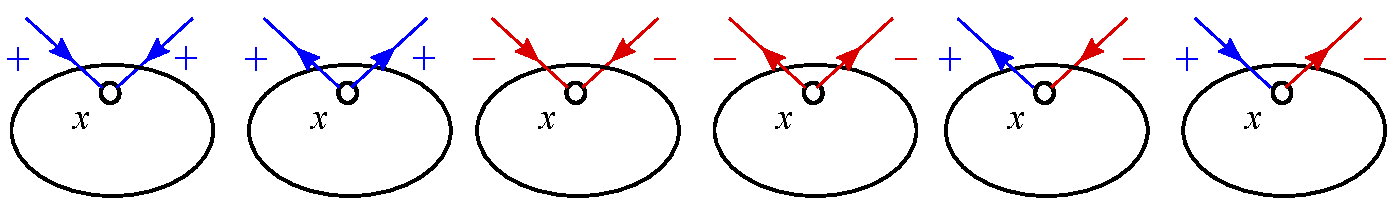
\includegraphics[width=13cm]{mismatch.pdf}} 
		%\ee
	\end{center}
	%Otherwise, if the two edges connected with $x$ are of the following  forms in the following figure, then we call them  {matched}:  
	%\hty{ Otherwise the two edges are  {matched} and of the following forms"}
	Otherwise the two edges are \emph{matched} and of the following forms:
	\begin{center}
		%\be\label{pic match}
		\parbox[c]{0.56\linewidth}{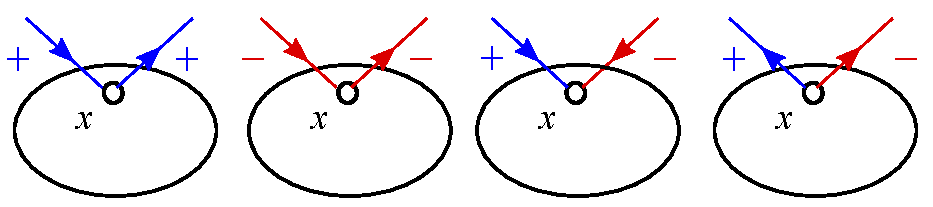
\includegraphics[width=9cm]{match.pdf}} 
		%\ee
	\end{center}
	In formulas, denoting the other ending atoms of the two edges by $y$ and $y'$, the two edges are matched if they are $G_{xy}G_{y'x}$, $\overline G_{xy}\overline G_{y'x}$, $G_{xy}\overline G_{xy'}$ or $G_{yx}\overline G_{y'x}$, that is, if they have the same charge and opposite orientations at $x$, or opposite charges and the same orientation at $x$; they are mismatched if they are $G_{xy}G_{xy'}$, $G_{yx}G_{y'x}$, $\overline G_{xy}\overline G_{xy'}$, $\overline G_{yx}\overline G_{y'x}$, $G_{xy}\overline G_{y'x}$ or $G_{yx}\overline G_{xy'}$.
	An atom is said to be \emph{standard neutral} if it is only connected to three edges besides possible $\times$-dotted edges: two {matched} $G$ edges of {opposite charges} and one waved $S$ edge. 
\end{definition}

The edges connected with a standard neutral atom almost form a $T$-variable (but not an exact $T$-variable because of $\times$-dotted edges; see Section \ref{subsec global} for more details).


%The above multi-edge expansion also motivates the following definition of \emph{matched} and \emph{mismatched} solid edges.
%Suppose an internal atom $x$ is of degree 2 in a graph $\cal G$. Then we can write $\cal G$ into one of the following forms: for some $y,y'\ne x$, 
%\be\label{mismatch direction} 
%\begin{split}
%	\cal G= \sum_{x,y,y'}G_{xy}   G_{x y'}  \Gamma_{x,yy'}, \quad \text{or}\quad \cal G= \sum_{x,y,y'}G_{yx}   G_{y'x}  \Gamma_{x,yy'}, \quad \text{or}\quad \cal G= \sum_{x,y,y'} G_{y x}   \overline G_{x y'}  \Gamma_{x,yy'},\\
%	\text{or}\quad \cal G= \sum_{x,y,y'} G_{xy}   \overline G_{ y' x}  \Gamma_{x,yy'},\quad \text{or}\quad \cal G=  \sum_{x,y,y'}\overline G_{xy}   \overline G_{ xy' }  \Gamma_{x,yy'}, \quad \text{or}\quad \cal G=  \sum_{x,y,y'}\overline G_{yx}   \overline G_{ y' x}  \Gamma_{x,yy'}, 
%\end{split}
%\ee
%or
%\be\label{match direction} \begin{split}
%	\cal G= \sum_{x,y,y'} G_{xy}   G_{y'x}  \Gamma_{x,yy'},  \quad \text{or}  \quad \cal G= \sum_{x,y,y'}G_{xy}   \overline G_{x y'}  \Gamma_{x,yy'}, \\
%	\text{or} \quad \cal G= \sum_{x,y,y'}G_{yx}   \overline G_{y' x}  \Gamma_{x,yy'},  \quad \text{or}  \quad  \cal G= \sum_{x,y,y'}\overline G_{xy}   \overline G_{y'x}  \Gamma_{x,yy'}.
%\end{split}\ee
%For cases in \eqref{mismatch direction}, we shall say that the two edges connected with $x$ are \emph{mismatched edges}, while for cases in \eqref{match direction}, we shall say that the two edges connected with $x$ are \emph{matched edges}. In the following figure, we have mismatched edges at $x$:
%\begin{center}
%	%\be\label{pic mismatch}
%	\parbox[c]{0.8\linewidth}{\includegraphics[width=14cm]{mismatch.png}} 
%	%\ee
%\end{center}
%In the following figure, we have matched edges at $x$:
%\begin{center}
%	%\be\label{pic match}
%	\parbox[c]{0.6\linewidth}{\includegraphics[width=10cm]{match.png}} 
%	%\ee
%\end{center}
%In Lemma \ref{expandmulti}, we will show that if $x$ is connected with two mismatched edges, then $\cal O_{multi-e}(x) \left[\cal G\right] $ is a sum of graphs that are of strictly higher scaling order than $\cal G$. For example, for the first term in \eqref{mismatch direction}, we have $k_1=2$ and $k_2=k_3=k_4=0$ in the setting of \eqref{multi setting}. Then the first two main terms on the right-hand side of \eqref{Oe1x} are both zero. 
 
%Recall \eqref{degree}, for any molecule $\cal M_i$, $\deg (\cal M_i)$ denotes the number of solid edges that connect the atoms in $\cal M_i$ to the atoms outside the molecule. 
  

 \begin{definition} [Locally standard graphs] \label{deflvl1} 
	A graph $\cal G$ is  \emph{locally standard}  if 
	\begin{itemize}
		\item[(i)] it is a normal regular graph without $P/Q$ labels; % (recall Definition \ref{defnlvl0});  
		
		%\item[(ii)] all the edges in the graph have no independent sets;
		
		%\item[(ii)] any two atoms in the same molecule are different, and there is a $\times$-dotted edge between them;
		
		\item[(ii)] it has no weights or light weights;
		
		\item[(iii)] the degree of any internal atom is $0$ or $2$; %(recall \eqref{degree}); %that is connected with solid $G$ edges must have degree 2 (at this step, the two edges can be of the same or different charges), and is connected with one waved $S$ edge;
		
		\item[(iv)] all degree 2 internal atoms are standard neutral. % (recall Definition \ref{def SNA}).%, that is, it is connected to exactly three edges---two {\bf matched} $G$ edges of {\bf opposite charges} and one waved $S$ edge---besides the $\times$-dotted edges. %if a internal atom is connected with two $G$ edges, then these two edges must be of opposite charges; 
		
		\end{itemize}
\end{definition}

Given a regular graph $\cal G$, we first apply $\cal O_{dot}$ to expand it into a linear combination of normal regular graphs, then apply the weight expansion to remove all weights, and then apply the multi-edge, $GG$ and $G\overline G$ expansions one by one to remove all atoms that are not standard neutral. In the end, we can expand $\cal G$ into a sum of locally standard graphs, recollision graphs, $Q$-graphs and higher order graphs. The following basic lemma on local expansions has been proved in \cite{PartI_high}.

\begin{lemma}[Lemma 3.22 of \cite{PartI_high}] \label{lvl1 lemma}
Let $\cal G_{\fa, \fb_1\fb_2}$ be a normal regular graph without solid edges connected with $\fa$, in which every weight or light weight is on an internal atom and every solid edge $G_{\al\beta}$ or $\overline G_{\al\beta}$ has an internal first index $\al$. Then for any fixed $n\in \N$, we have that
\begin{align}\label{expand lvl1}
\cal G_{\fa, \fb_1\fb_2} =  (\cal G_{local})_{\fa, \fb_1\fb_2}  + \PGn_{\fa,\fb_1\fb_2} +  (\AGn)_{\fa,\fb_1\fb_2} + \QGn_{\fa,\fb_1\fb_2} ,
\end{align}
where $(\cal G_{local})_{\fa, \fb_1\fb_2} $ is a sum of $\OO(1)$ many locally standard graphs, \smash{$ \PGn_{\fa,\fb_1\fb_2} $} is a sum of $\OO(1)$ many $\oplus$/$\ominus$-recollision graphs, \smash{$(\AGn)_{\fa,\fb_1\fb_2}$} is a sum of $\OO(1)$ many graphs of scaling order $> n$, and \smash{$(\QGn)_{\fa,\fb_1\fb_2} $} is a sum of $\OO(1)$ many $Q$-graphs.  Every molecule in a graph on the right-hand side is obtained by merging some molecules in the original graph $\cal G_{\fa, \fb_1\fb_2}$. 
\end{lemma}

%\begin{remark}

%We have  noted that  local expansions will not create new molecules. Hence 
If there are no dotted or waved edges added  between different molecules, then the molecules in a new graph are the same as those  in $\cal G_{\fa, \fb_1\fb_2}$. In general, there may be newly added dotted edges (due to the dotted edge partition $\cal O_{dot}$) or waved edges (due to the first term on the right-hand side of \eqref{Oe2x}), so the molecules in a new graph are obtained from merging the molecules connected by dotted or waved edges. Now we show that local expansions do not break the doubly-connected property.

\begin{lemma}\label{lem localgood}
Suppose a normal regular graph $\cal G$ %without external molecules 
is doubly-connected in the sense of Definition \ref{def 2net}. Then applying any expansion in Definitions \ref{dot-def}, \ref{Ow-def}, \ref{multi-def}, \ref{GG-def} or \ref{GGbar-def} to $\cal G$, where the $GG$ expansion is applied as in Step 1 of Strategy \ref{strat_global}, that is, in the form whose waved edge in the leading term joins $x$ to an internal atom, the new graphs (including the $Q$-graphs) are all doubly connected normal regular graphs. % in the sense of Definition \ref{def 2net} with external molecules removed.   
 \end{lemma}
 \begin{proof}
%Using the definitions of local expansions, it is easy to check that all the new graphs are regular. The less trivial part of the proof is to show that the property (iii) of Definition \ref{defnlvl0} holds for the integration by parts graphs. Here we shall use the fact that $\partial_{\overline h_{\al\beta}}f_x(G)$ contains two edges connected with atoms $\al$ and $\beta$, respectively,  which are generated from taking the partial derivative $\partial_{\overline h_{\al\beta}}$ of a $G$ edge or $G$ weight. 
% Then we show the doubly connected property for all the new graphs in the local expansions. 
%The following discussions focus on the molecular graphs. 
First, all blue solid and (labelled) $\dashed$ edges between molecules are all unchanged in a dotted edge partition. The only changes are that in new molecular graphs, some molecules are merged into one molecule due to newly added dotted edges between different molecules. It is obvious that such merging operations will not break the doubly connected property. 
%we only add new dotted lines to the graphs or remove $\times$-dotted lines. Hence the doubly connected property is not affected.

Then we consider the weight expansion in Definition \ref{Ow-def}. It is trivial to see that \smash{${\cal O}^{(x),1}_{weight}$} does not change molecular graphs at all. Hence it remains to show that \smash{${\cal O}^{(x),2}_{weight}[\cal G]$} of a doubly connected graph $\cal G$ is still a sum of doubly connected graphs. Let $\cal G_1$ be one of the new graphs. Since new atoms are all included into the molecule containing $x$, the molecules in the molecular graph of $\cal G_1$ are the same as those in the original molecular graph of $\cal G$. Moreover, (labelled) $\dashed$ edges between molecules are also not affected, i.e. the black net does not change. It remains to consider the plus $G$ edges between molecules in $\cal G_1$. From \eqref{Owx}, it is easy to see that any plus $G$ edge in the molecular graph of $\cal G$ between two different molecules, say $\cal M_1$ and $\cal M_2$, either is not affected or becomes a connected path of two plus $G$ edges between $\cal M_1$ and $\cal M_2$ due to the partial derivatives $\partial_{h_{ \al x}}$ or $\partial_{h_{\beta\al}}$. (For example, if the atoms $x$, $\al$ and $\beta$ are in molecule $\cal M_3$, then the edge between $\cal M_1$ and $\cal M_2$ becomes two plus $G$ edges from $\cal M_1$ to $\cal M_3$ and from $\cal M_3$ to $\cal M_2$.) In either case, the path connectivity of the blue net is not affected, and hence the doubly connected property preserves in $\cal G_1$.

%{\cor For the local expansion in Definitions \ref{Ow-def}, \ref{multi-def}, \ref{GG-def} and \ref{GGbar-def}, the new atoms like $\al$ and $\beta$ are connected to atom $x$ through a path of waved $s$ and $S^{\pm}$ edges, and hence they are included into the molecule containing $x$. This shows that the molecules in the new molecular graphs of these local expansions are the same molecules as in the original molecular graph of $\cal G$. On the one hand, the labelled $\dashed$ edges between molecules are not affected in these expansions. On the other hand, any  plus $G$ edge in the molecular graph of  $\cal G$ between two different molecules, say $\cal M_1$ and $\cal M_2$, is either not affected or becomes a connected path of two plus $G$ edges between $\cal M_1$ and $\cal M_2$ due to the partial derivatives $\partial_{\overline h_{x\al}}$ or $\partial_{\overline h_{\al\beta}}$. (For example, if the atoms $x$, $\al$ and $\beta$ are in molecule $\cal M_3$, then this edge between $\cal M_1$ and $\cal M_2$ becomes two plus $G$ edges from $\cal M_1$ to $\cal M_3$ and from $\cal M_3$ to $\cal M_2$.) In either case, the path connectivities of both the blue net and the black net (in the molecular graph) are not affected, and hence the doubly-connected property still holds.}

For the edge expansions in Definitions \ref{multi-def}, \ref{GG-def} and \ref{GGbar-def}, the argument is exactly the same. The transposed form of the $GG$ expansion in Definition \ref{GG-def} (used when $y$ is an external atom) is the case of an internal $y$ with $y'$ in place of $y$.
 \end{proof}

\subsection{Global expansions}\label{subsec global}

In this section, we define global expansions. As an induction hypothesis, suppose we have obtained the $(n-1)$-th order $T$-expansion.  Then a global expansion of a locally standard graph, say $\cal G$, consists of the following three steps:
\begin{itemize}
	\item[(i)] we choose a standard neutral atom in $\cal G$;
	\item[(ii)] we replace the $T$-variable containing the atom in (i) by the $(n-1)$-th order $T$-expansion;
	\item[(iii)] we apply $Q$-expansions to every resulting graph with $Q$-labels from (ii).
\end{itemize}
We call this procedure ``global" because it may create new molecules in our graphs. %For example, if we replace a $T_{x,y_1y_2}$ with the right-hand side of \eqref{Otheta} (with $f(G)\equiv 1$), then the new atoms $\al$ and $\beta$ are in a different molecule from $x$. 
Unlike local expansions, a global expansion may break the doubly connectedness of graphs. To avoid this issue, %To preserve the double-net structures, 
we need to follow a specific criterion in choosing the standard neutral atom in (i). This will be discussed in Section \ref{sec pre}. %We remark that the estimate \eqref{intro_redagain} is needed to bound the graphs in global expansions. This is a reason why the $\renormal$ is needed. 
%have to use the sum zero properties \eqref{3rd_property0} and \eqref{weaz} in an essential way, and 
%apply the global expansions according to a carefully chosen order. We will deal with this issue in \cite{PartII_high}, and we refer the reader to Section \ref{sec strategy} for a brief discussion. 
%Note that the graphs obtained from the global expansions cannot be bounded properly unless we  know the $\renormal$. 
%Then we only use one type of global expansion, that is, replacing a $T$-variable with the $(n-1)$-th order $T$-expansion.
In this subsection, we define step (ii) in the above procedure, and postpone the definition of $Q$-expansions in step (iii) to the next subsection. 


Picking a standard neutral atom, say $\al$, in a locally standard graph, the edges connected to it take one of the following forms:
\begin{equation}\label{12in4T}
	t_{x,y_1 y_2} :=|m|^2\sum_\al s_{x\al}G_{\al y_1}\overline G_{\al y_2}\mathbf 1_{\al\ne y_1}\mathbf 1_{\al\ne y_2},\quad \text{or}\quad t_{y_1y_2, x}:=|m|^2\sum_\al G_{ y_1\al }\overline G_{y_2 \al}s_{\al x}\mathbf 1_{\al\ne y_1}\mathbf 1_{\al\ne y_2} .
\end{equation}
Then we apply the $(n-1)$-th order $T$-expansion in \eqref{mlevelTgdef} to these variables in the following way: %take $ t_{x,y_1 y_2} $ as an example,
\begin{align*}
	t_{x,y_1 y_2} & = m  \Theta_{xy_1}\overline G_{y_1y_2} +m (\Theta \Sdelta^{(n-1)}\Theta)_{xy_1} \overline G_{y_1y_2} + (\PT^{(n-1)})_{x,y_1 y_2} +  (\AT^{(>n-1)})_{x,y_1y_2}  + (\QT^{(n-1)})_{x,y_1y_2} \nonumber\\
	& +  (\Err_{n-1,D})_{x,y_1y_2}  - |m|^2\sum_\al s_{x\al}G_{\al y_1}\overline G_{\al y_2}\left(\mathbf 1_{\al\ne y_1}\mathbf 1_{\al = y_2}+\mathbf 1_{\al=y_1}\mathbf 1_{\al \ne y_2} +\mathbf 1_{\al = y_1}\mathbf 1_{\al = y_2}\right) .
\end{align*}
%Note that $\mathbf 1_{\al = y_1}\mathbf 1_{\al = y_2} =0$ if $y_1\ne y_2$, and $\mathbf 1_{\al\ne y_1}\mathbf 1_{\al = y_2} =\mathbf 1_{\al=y_1}\mathbf 1_{\al \ne y_2}=0$ if $y_1= y_2$. 
The last term on the right-hand side gives one (since $\mathbf 1_{\al\ne y_1}\mathbf 1_{\al = y_2} =\mathbf 1_{\al=y_1}\mathbf 1_{\al \ne y_2}=0$ if $y_1= y_2$) or two (since $\mathbf 1_{\al = y_1}\mathbf 1_{\al = y_2} =0$ if $y_1\ne y_2$) recollision graphs, so we combine it with {$ (\PT^{(n-1)})_{x,y_1 y_2}$} and denote the resulting term by {$(\wtPT^{(n-1)})_{x,y_1 y_2}$}. Hence we get the following expansion formula of the $t$-variable $t_{x,y_1 y_2}$:
\begin{align}
	t_{x,y_1 y_2} &=   m  \Theta_{xy_1}\overline G_{y_1y_2} +m   (\Theta \Sdelta^{(n-1)}\Theta)_{xy_1} \overline G_{y_1y_2}  +  (\wtPT^{(n-1)})_{x,y_1 y_2} +  (\AT^{(>n-1)})_{x,y_1y_2}  \nonumber\\
	& + (\QT^{(n-1)})_{x,y_1y_2} +  (\Err_{n-1,D})_{x,y_1y_2} .\label{replaceT}
\end{align}
The expansion of $t_{y_1y_2, x}$ is obtained from \eqref{replaceT} by transposing all $G$ entries. In fact, $H^\top$ satisfies the same assumptions as $H$ (with variances $s_{yx}=s_{xy}$) and its resolvent is $G^\top$, so \eqref{replaceT} also holds with $G$ replaced by $G^\top$; the waved edges, the $\dashed$ edges and the labelled $\dashed$ edges are functions of $S$ and are not transposed.

\subsection{$Q$-expansions}\label{sec defnQ}

If we replace a $t$-variable with a graph in $\QT^{(n-1)}$, then we will get a graph of the form  
\be\label{QG}\cal G_0=\sum_x \Gamma_0 Q_x (\wt\Gamma_0) ,\ee
where both the graphs $\Gamma_0$ and $\wt\Gamma_0$ do not contain $P/Q$ labels. The $Q$-expansions defined  in this subsection aim to expand the above graph into a sum of $Q$-graphs and graphs without $P/Q$ labels.  By Definition \ref{Def_recoll}, $Q$-graphs refer to graphs where all edges and weights have the same $Q$-label. The graph $\cal G_0$ does not satisfy this property, so we will not call it a $Q$-graph to avoid confusion. 

\medskip
\noindent{\bf Step 1:} First, for every atom $u\ne x$ that is an ending atom of a solid edge or carries a weight in $\Gamma_0$ and is not connected with $x$ through a $\times$-dotted edge, we write $1=\mathbf 1_{u=x}+\mathbf 1_{u\ne x}$, i.e., we add a dotted or a $\times$-dotted edge between $u$ and $x$; in a graph with $u=x$, the solid edges and weights at $u$ are regarded as attached to $x$. Then we apply \smash{${\cal O}^{(x),1}_{weight} \circ\cal O_{dot}$} to the resulting graphs and get a sum of normal regular graphs without regular weights on atom $x$. Now for any new graph, say $\cal G=\sum_x \Gamma Q_x (\wt \Gamma), $ if $\Gamma$ does not contain any light weight or edges attached to $x$, then we apply the following operations. In this case, every atom of a solid edge or a weight in $\Gamma$ is connected with $x$ through a $\times$-dotted edge, so \eqref{resol_exp0} below is applied only to entries $G_{x_1x_2}$ with $x_1,x_2\ne x$. (The above splitting has to be performed first: if an atom with two or more light weights were identified with $x$ only after the operations \eqref{resol_exp0}, \eqref{resol_reverse} and \eqref{weight_taylor} below, the scaling order could decrease.)


Let $H^{(x)}$ be the $(N-1)\times(N-1)$ minor of $H$ obtained by removing the $x$-th row and column of $H$, and define the resolvent minor $G^{(x)}(z):=(H^{(x)}-z)^{-1}$. The following resolvent identity is well-known:
\be\label{resol_exp0}G_{x_1x_2}=G_{x_1x_2}^{(x)}+\frac{G_{x_1 x}G_{xx_2}}{G_{xx}},\quad x_1,x_2\in \Z_L^d,\ee
which follows from the Schur complement formula. Correspondingly, we introduce a new type of weights, $(G_{xx})^{-1}$ and $(\overline G_{xx})^{-1}$, and a new label $(x)$ to solid edges and weights. More precisely, if a weight on $x$ has a label ``$(-1)$", then this weight represents a $(G_{xx})^{-1}$ or $(\overline G_{xx})^{-1}$ factor depending on its charge; if an edge or a weight has a label $(x)$, then it represents a $G^{(x)}$ entry. 

Applying \eqref{resol_exp0} to expand the resolvent entries in $\Gamma$ one by one, we can get that
\be\label{decompose_gamma} \Gamma=\Gamma^{(x)}+\sum_{\omega} \Gamma_\omega,\ee 
where $\Gamma^{(x)}$ is a graph whose weights and solid edges all have the $(x)$ label, and hence is independent of the $x$-th row and column of $H$. The second term on the right-hand side of \eqref{decompose_gamma} is a sum of $\OO(1)$ many graphs. More precisely, let $g_1,\ldots,g_r$ be the solid edges and weights of $\Gamma$, listed in a fixed order, and let $g_i=g_i^{(x)}+\delta_i$ be the decomposition of $g_i$ given by \eqref{resol_exp0}. Then $\Gamma^{(x)}$ is obtained by replacing every $g_i$ with $g_i^{(x)}$, and the graphs $\Gamma_\omega$, $1\le \omega\le r$, are obtained by replacing $g_1,\ldots,g_{\omega-1}$ with $g_1^{(x)},\ldots,g_{\omega-1}^{(x)}$ and $g_\omega$ with $\delta_\omega$. Moreover, every $\Gamma_\omega$ has a strictly higher scaling order than $\Gamma$, at least two new solid edges connected with $x$, and some weights with label $(-1)$ on $x$. Using \eqref{decompose_gamma}, we can expand $\cal G$ as
\be\label{QG2}
\cal G=\sum_x \Gamma Q_x (\wt \Gamma)=\sum_{\omega}\sum_x \Gamma_\omega Q_x(\wt \Gamma) + \sum_x Q_x ( \Gamma \wt\Gamma )- \sum_{\omega}\sum_x Q_x (\Gamma_\omega \wt\Gamma ),
\ee
where the second and third terms are sums of $Q$-graphs.


Next, we expand graphs $\Gamma_\omega$ in \eqref{QG2} into graphs without $G^{(x)}$, $(G_{xx})^{-1}$ or $(\overline G_{xx})^{-1}$ entries. First, we apply the following expansion to the $G^{(x)}$ entries in $\Gamma_{\omega}$: 
\be\label{resol_reverse}G_{x_1x_2}^{(x)}= G_{x_1x_2} - \frac{G_{x_1 x}G_{xx_2}}{G_{xx}}. \ee
In this way, we can write $\Gamma_{\omega}$ as a sum of graphs \smash{$\sum_{\zeta} \Gamma_{\omega,\zeta}$}, where $\Gamma_{\omega,\zeta}$ does not contain any $G^{(x)}$ entries. Second, we expand the $(G_{xx})^{-1}$ and $(\overline G_{xx})^{-1}$ weights in $\Gamma_{\omega,\zeta}$ using the Taylor expansion
\be\label{weight_taylor}\frac{1}{G_{xx}}=\frac{1}{m} + \sum_{k=1}^{D}\frac1m\left(-\frac{G_{xx}-m}{m}\right)^k + \cal W^{(x)}_{D},\quad \cal W^{(x)}_{D}:=\frac{1}{G_{xx}}-\sum_{k=0}^{D}\frac1m\left(-\frac{G_{xx}-m}{m}\right)^k=\frac{1}{G_{xx}}\left(-\frac{G_{xx}-m}{m}\right)^{D+1} . \ee
When $|G_{xx}-m|<|m|$, we have $\cal W^{(x)}_{D}=m^{-1}\sum_{k>D}(-(G_{xx}-m)/m)^k$. We will regard $\cal W^{(x)}_{D}$ and $\overline{\cal W}^{(x)}_{D}$ as a new type of weights of scaling order $D+1$. (If necessary, we replace $D$ in \eqref{weight_taylor} by a larger integer depending only on $D$ and the scaling order of the graph, so that every graph containing such a weight has scaling order $>D$.) Expanding the product of all Taylor expansions of the $(G_{xx})^{-1}$ and $(\overline G_{xx})^{-1}$ weights, we can write every $\Gamma_{\omega,\zeta}$ into a sum of graphs that do not contain weights with label $(-1)$. %Note that the graphs containing {$\cal W^{(x)}_{D}$ or $\overline{\cal W}^{(x)}_{D}$} can be included into the error term $\Err_{n,D}$ in \eqref{mlevelTgdef}. 
Finally, applying \smash{${\cal O}^{(x),1}_{weight} \circ\cal O_{dot}$} again, we will get a sum of normal regular graphs without regular weights on $x$. 

Now we summarize Step 1 in the following lemma. 
\begin{lemma}\label{Q_lemma1}
Given a normal regular graph taking the form \eqref{QG}, we can expand it into a sum of $\OO(1)$ many graphs: %as In sum, in Step 1 we expand \eqref{QG} as 
\be\label{Q_eq1}\cal G_0 = \sum_{\omega} \Gamma_\omega Q_x(\wt \Gamma_{\omega}) + \sum_{\zeta} Q_x \left( \cal G_\zeta \right) + \cal G_{err},\ee
where $\Gamma_{\omega}$, $\wt \Gamma_{\omega}$ and $\cal G_\zeta $ are normal regular graphs without $P/Q$, ${(x)}$ or $(-1)$ labels, and $\cal G_{err}$ is a sum of normal regular graphs of scaling order $>D$.  %Moreover, every $\Gamma_\omega$ contains light weights or edges attached to the atom $x$. 
%\hty{ change to 
%where $\Gamma_{\omega}$, $\wt \Gamma_{\omega}$ and $\cal G_\zeta $ are normal regular graphs without $P/Q$-labels and $\cal G_{err}$ is a sum of normal regular graphs of scaling order $>D$. Notice that by definition of normal regular graphs, $\Gamma_{\omega}$, $\wt \Gamma_{\omega}$ and $\cal G_\zeta $ do not contain any 
% $G^{(x)}$ entries, or $(G_{xx})^{-1}$ or  $(\overline G_{xx})^{-1}$ weights. } 
If $\Gamma_0$ does not contain any weights or edges attached to $x$, then every $\Gamma_\omega$ has a strictly higher scaling order than $\Gamma_0$ and contains at least one atom which either is connected to $x$ through a solid edge or has been merged with $x$.

%one atom that satisfies one of the following properties: it is connected to $x$ through solid edges; it has been merged with $x$.
%\hty{ one atom which  either is connected to $x$ through a solid edge or  it has been merged with $x$. There are similar sentences in the following which should be also corrected.} 
\end{lemma}
\begin{proof} 
We only need to prove the second statement. Suppose $\Gamma_0$ does not contain any weights or edges attached to $x$. If $\Gamma_\omega$ comes from a graph with $u=x$ in the splitting at the beginning of Step 1, then the atom $u$ of $\Gamma_0$ has been identified with $x$ (merged with $x$ if $u$ is internal, or connected with $x$ through a dotted edge if $u$ is external), which increases the scaling order by $2$. Otherwise, there exists at least one $G_{x_1x_2}$ or $\overline G_{x_1x_2}$ entry in $\Gamma_0$ that has been replaced by two solid edges $G_{x_1 x}G_{xx_2}$ or $\overline G_{x_1 x}\overline G_{x x_2}$ (together with a $(G_{xx})^{-1}$ or $(\overline G_{xx})^{-1}$ weight). These two solid edges will either appear in $\Gamma_{\omega}$ or become weights if $x_1$ or $x_2$ is identified with $x$ due to newly added dotted edges in $\cal O_{dot}$ operations. 
\end{proof}
If $\Gamma_0$ does not contain any weights or edges attached to $x$, then after Step 1 the structures of $\Gamma_\omega$ in \eqref{Q_eq1} are already good enough for our purpose. In Steps 2 and 3, we aim to remove the $Q_x$ label in $Q_x(\wt \Gamma_{\omega})$.

\medskip   

\noindent{\bf Step 2:} In this step and Step 3, we will remove the $Q_x$ label in  
$$\Gamma_\omega Q_x(\wt \Gamma_{\omega})=\Gamma_\omega \wt \Gamma_{\omega} - \Gamma_\omega P_x(\wt \Gamma_{\omega}).$$
It suffices to write $P_x (\wt \Gamma_{\omega})$ into a sum of graphs without the $P_x$ label. To this end, we will use the following lemma. 

\begin{lemma}
Let $f$ be a differentiable function of $G$. %For a graph $\cal G=(G_{xx}  -  m) f(G)$, 
We have that
\begin{align}
	  P_x \left[(G_{xx}  -  m) f(G)\right] &=  P_x\Big[ m^2 \sum_{\al} s_{x\al} (G_{\al\al}-m)  f(G) + m \sum_{\al} s_{x\al} (G_{\al\al}-m) (G_{xx}-m)f(G)\Big] \nonumber\\
	& -  P_x  \Big[  m \sum_\al s_{x\al} G_{\al x}\partial_{  h_{\al x}} f(G)\Big]. \label{gHw}
\end{align}
Given a graph $\cal G$ taking the form \eqref{multi setting}, we have the following identity if $k_1\ge 1$:
\begin{align} 
	  P_x[\cal G]   &= \sum_{i=1}^{k_2}|m|^2 P_x \left[  \left( \sum_\al s_{x\al }G_{\al y_1} \overline G_{\al y'_i}\right)\frac{\cal G}{G_{x y_1} \overline G_{xy_i'}} \right] + \sum_{i=1}^{k_3} m^2 P_x \left[ \left(\sum_\al s_{x\al }G_{\al y_1} G_{w_i \al} \right)\frac{\cal G}{G_{xy_1}G_{w_i x}}\right] \nonumber \\
	 & + \sum_{i=1}^{k_2}m P_x \left[ \left(\overline G_{xx} -\overline m\right) \left( \sum_\al s_{x\al }G_{\al y_1} \overline G_{\al y'_i}\right)\frac{\cal G}{G_{x y_1} \overline G_{xy_i'}} \right] \nonumber\\
	 &+ \sum_{i=1}^{k_3} m P_x \left[ (G_{xx}-m) \left(\sum_\al s_{x\al }G_{\al y_1} G_{w_i \al} \right)\frac{\cal G}{G_{xy_1}G_{w_i x}}\right] \nonumber \\
	&+  m P_x \left[  \sum_\al s_{x\al }\left(G_{\al \al}-m\right) \cal G\right] +(k_1-1) m P_x \left[  \sum_\al s_{x\al }G_{\al y_1} G_{x \al} \frac{ \cal G}{G_{xy_1}}\right] \nonumber\\
	&+ k_4 m P_x \left[  \sum_\al s_{x\al }G_{\al y_1} \overline G_{\al x} \frac{\cal G}{G_{xy_1}}\right]  - m P_x \left[  \sum_\al s_{x\al }\frac{\cal G}{G_{x y_1}f(G)}G_{\al y_1}\partial_{ h_{\al x}}f (G)\right].\label{gH0} 
	% & - m P_x \left[  \sum_\al s_{x\al }G_{\al y_1}\cdot \prod_{i=2}^{k_1}G_{x y_i}  \cdot  \prod_{i=1}^{k_2}\overline G_{x y'_i} \cdot \prod_{i=1}^{k_3} G_{ w_i x} \cdot \prod_{i=1}^{k_4}\overline G_{ w'_i x}\cdot \partial_{ h_{ \al x}}f(G)\right]+ Q_x \left(  \cal G\right)  .
\end{align} 
\end{lemma}
\begin{proof}
These two identities both follow from Gaussian integration by parts, and have been proved in Lemma 3.5 and Lemma 3.10 of \cite{PartI_high}.
\end{proof}

Similar to Definition \ref{Ow-def}, we can define an operator $\wt{\cal O}^{(x)}_{weight}$ acting on a graph $P_x(\cal G)$ as 
$$	\wt{\cal O}_{weight}^{(x)}[ P_x(\cal G)]:={\cal O}^{(x),1}_{weight} \circ\cal O_{dot} \circ  \wt{\cal O}^{(x),2}_{weight} \circ {\cal O}^{(x),1}_{weight}  [P_x(\cal G)],$$
where $\wt{\cal O}^{(x),2}_{weight}$ is an operator defined from \eqref{gHw}. Also similar to Definition \ref{multi-def}, we can define an operator \smash{$\wt{\cal O}^{(x)}_{multi-e}$} acting on a graph $P_x(\cal G)$ as 
$$\wt{\cal O}_{multi-e}^{(x)}[ P_x(\cal G) ]:= \cal O_{dot} \circ  \wt{\cal O}_{multi-e}^{(x),1} [P_x(\cal G)], $$ 
where $\wt{\cal O}_{multi-e}^{(x),1}$ is an operator defined from \eqref{gH0} (the $k_1=0$ case can be handled in the same way as cases (ii)--(iv) of Definition \ref{multi-def} and we omit the details).

%We will apply the $\wt{\cal O}_{weight}^{(x)}$ and $\wt{\cal O}^{(x),2}_{weight}$ repeatedly to expand $P_x (\wt \Gamma_{\omega})$. 

If a normal regular graph $P_x(\cal G)$ contains weights or solid edges attached to $x$, then we will apply \smash{$\wt{\cal O}_{weight}^{(x)}$ or $\wt{\cal O}^{(x)}_{multi-e}$} to it. We repeat these operations until all graphs do not contain weights or solid edges attached to $x$, and hence obtain the following lemma. 


\begin{lemma}\label{Q_lemma2}
Suppose $\cal G$ is a normal regular graph without $P/Q$, $(x)$ or $(-1)$ labels. % $G^{(x)}$ entries, and $(G_{xx})^{-1}$ or $(\overline G_{xx})^{-1}$ weights. 
Then we can expand $P_x(\cal G)$ into a sum of $\OO(1)$ many graphs: 
$$P_x(\cal G) = \sum_{\omega}  P_x(\cal G_{\omega}) +  \cal G_{err}\ ,$$
where $\cal G_{\omega}$ are normal regular graphs without weights or edges attached to $x$ (and without $P/Q$, $(x)$ or $(-1)$ labels), and $\cal G_{err}$ is a sum of normal regular graphs of scaling order $>D$. 
\end{lemma}
\begin{proof}
We only describe the main argument for the proof without writing down all the details. Given a normal regular graph $P_x(\cal G)$, it is easy to check that every graph in \smash{$\wt{\cal O}_{weight}^{(x)}[P_x(\cal G)]$ or $\wt{\cal O}^{(x)}_{multi-e}[P_x(\cal G)]$}, say $P_x(\cal G_1)$, satisfies one of the following properties:
\begin{itemize}
	\item $P_x(\cal G_1)$ has a strictly higher scaling order than $P_x(\cal G)$;
	\item $P_x(\cal G_1)$ has the same scaling order as $P_x(\cal G)$, and a strictly smaller weighted number of weights and edges attached to $x$, where every light weight on $x$ counts $4$, every regular weight on $x$ counts $1$, and every end of a solid edge at $x$ counts $1$.
\end{itemize}
(The unweighted number of weights and edges attached to $x$ may not decrease: if $\cal G=(G_{xx}-m)^2\cal G'$, then $\wt{\cal O}^{(x)}_{weight}[P_x(\cal G)]$ contains the graph $m^2 P_x[\sum_\al s_{x\al}\mathbf 1_{\al\ne x}G_{\al x}G_{x\al}\cal G']$, which has the same scaling order as $P_x(\cal G)$ and two edges attached to $x$.)
Hence applying the operations \smash{$\wt{\cal O}_{weight}^{(x)}$ or $\wt{\cal O}^{(x)}_{multi-e}$} for $C_{\cal G, D}$ many times,  each resulting graph either is of scaling order $>D$, or has no weights or edges attached to $x$. Here $C_{\cal G, D}\in \N$ is a large constant depending only on $D$ and the number of weights and edges attached to atom $x$ in $\cal G$.
\end{proof}

With Lemma \ref{Q_lemma2}, in Step 2 we can expand $Q_x(\wt \Gamma_{\omega})$ as
\be\label{PxGamma} Q_x(\wt \Gamma_{\omega})=   \wt \Gamma_{\omega} - \sum_{\zeta}P_x(\wt \Gamma_{\omega,\zeta}) + \cal G_{err},\ee
where $\wt\Gamma_{\omega,\zeta}$ are normal regular graphs without weights or edges attached to $x$, and $\cal G_{err}$ is a sum of graphs of scaling order $>D$.  


\medskip
\noindent{\bf Step 3:} In this step, we expand the graphs $P_x(\wt \Gamma_{\omega,\zeta})$ in \eqref{PxGamma}. Suppose $\cal G$ is a normal regular graph without weights or edges attached to $x$. As in Step 1, we first write $1=\mathbf 1_{u=x}+\mathbf 1_{u\ne x}$ for every atom $u$ of a solid edge or a weight in $\cal G$ that is not connected with $x$ through a $\times$-dotted edge, and apply \smash{${\cal O}^{(x),1}_{weight} \circ\cal O_{dot}$}. The graphs with $u=x$ have strictly higher scaling orders than $\cal G$, and we apply the present step again to those of them that have no light weights or edges attached to $x$. Hence we can assume that every atom of a solid edge or a weight in $\cal G$ is connected with $x$ through a $\times$-dotted edge. Using the resolvent identity \eqref{resol_exp0}, we can write $\cal G$ into a similar form as in \eqref{decompose_gamma}:
$$\cal G = \cal G^{(x)} + \sum_\omega \cal G_{\omega},$$
where $\cal G^{(x)}$ is a graph whose weights and solid edges all have the same $(x)$ label, and every graph $\cal G_{\omega}$ has a strictly higher scaling order than $\cal G$, at least two new solid edges connected with $x$, and some weights with label $(-1)$ on $x$. Then we can expand $P_x(\cal G)$ as 
$$P_x(\cal G) = \cal G- \sum_\omega \cal G_{\omega} + \sum_\omega P_x(\cal G_{\omega}).$$
Next, as in Step 1, we apply \eqref{resol_reverse} and \eqref{weight_taylor} to remove all $G^{(x)}$, $(G_{xx})^{-1}$ and $(\overline G_{xx})^{-1}$ entries from $\cal G_{\omega}$. Finally, we apply \smash{${\cal O}^{(x),1}_{weight} \circ\cal O_{dot}$} to all resulting graphs to get a sum of normal regular graphs without regular weights on $x$. In sum, we obtain the following result. 

\begin{lemma}\label{Q_lemma3}
Suppose $\cal G$ is a normal regular graph without $P/Q$, $(x)$ or $(-1)$ labels. Moreover, suppose $\cal G$ has no weights or edges attached to $x$. Then we can expand $P_x(\cal G)$ into a sum of $\OO(1)$ many graphs: 
$$P_x(\cal G) = \cal G+ \sum_\xi  \cal G_{\xi}  + \sum_\gamma  P_x(\wt{\cal G}_{\gamma}) + \cal G_{err},$$
where \smash{$\cal G_{\xi}$ and $\wt{\cal G}_{\gamma}$} are normal regular graphs without $P/Q$, $(x)$ or $(-1)$ labels, and $\cal G_{err}$ is a sum of normal regular graphs of scaling order $>D$. Moreover, $\cal G_\xi$ and $\wt{\cal G}_{\gamma}$ are of strictly higher scaling order than $\cal G$, and have light weights or edges attached to the atom $x$.
\end{lemma}

With this lemma, we can expand $P_x(\wt \Gamma_{\omega,\zeta}) $ in \eqref{PxGamma} as
$$P_x(\wt \Gamma_{\omega,\zeta}) =\wt \Gamma_{\omega,\zeta}+ \sum_\xi  \Gamma_{\omega,\zeta,\xi} + \sum_\gamma  P_x (\wt \Gamma_{\omega,\zeta,\gamma} ) +\cal G_{err},$$
where $\Gamma_{\omega,\zeta,\xi}$ and $\wt \Gamma_{\omega,\zeta,\gamma} $ respectively satisfy the same properties as 
$ \cal G_{\xi}$ and $\wt{\cal G}_{\gamma} $ in Lemma \ref{Q_lemma3}. Then we apply Step 2 to the graphs $P_x(\wt \Gamma_{\omega,\zeta,\gamma} )$ again. Repeating Steps 2 and 3 for $\OO(1)$ many times, we can finally expand $P_x (\wt \Gamma_{\omega})$ into a sum of graphs without $P_x$ labels plus graphs of scaling order $>D$. 

\medskip
 
Combining Steps 1--3, we obtain the following lemma on $Q$-expansions. 

\begin{lemma}[$Q$-expansions]\label{Q_lemma}
Suppose $\Gamma_0$ and $\wt\Gamma_0$ in \eqref{QG} are normal regular graphs without $P/Q$, $(x)$ or $(-1)$ labels. %\hty{ this sentence should be corrected as previous one. We already said that normal regular graph cannot contain any $G^{(x)}$, $(G_{xx})^{-1}$ or $(\overline G_{xx})^{-1}$ labels. Isn't it?  } 
Then $\cal G_0$ can be expanded into a sum of $\OO(1)$ many graphs:
\be\label{G0Q} \cal G_0 = \sum_\omega \cal G_\omega + \sum_\zeta Q_x(\wt{\cal G}_\zeta)  + \cal G_{err},\ee
where $\cal G_{\omega}$ and $\wt{\cal G}_\zeta$ are normal regular graphs without $P/Q$, $(x)$ or $(-1)$ labels, and $\cal G_{err}$ is a sum of normal regular graphs of scaling order $>D$. Moreover, these graphs satisfy the following properties.
\begin{itemize}
	\item[(i)] Every graph on the right-hand side of \eqref{G0Q} has a scaling order $\ge \ord(\cal G_0)$.
	
	\item[(ii)] If there is a new atom in a graph on the right-hand side of \eqref{G0Q}, then it is connected to $x$ through a path of waved edges. Hence the expansion \eqref{G0Q} is a local expansion. 
	
	\item[(iii)] If $\cal G_0$ is doubly connected, then all graphs on the right-hand side of \eqref{G0Q} are also doubly connected.
	
	\item[(iv)] If $\Gamma_0$ does not contain any weights or edges attached to $x$, then the scaling order of  $\cal G_\omega$ is  strictly higher than $\ord(\cal G_0)$ for every $\omega$.
	%then each $\cal G_\omega$ is of strictly higher scaling order than $\cal G_0$. \hty{ 	then the scaling order of  $\cal G_\omega$ is  strictly higher  than that of $\cal G_0$ for every $\omega$. } 
 Furthermore,  $\cal G_\omega$ contains at least one atom that belongs to the original graph $\Gamma_0$ and satisfies the following property: it is connected to $x$ through a solid edge or it has been merged with $x$. More precisely, up to the identification of atoms through dotted edges, every weight and solid edge of $\Gamma_0$ appears in $\cal G_\omega$ either unchanged or \emph{split at $x$}, i.e., replaced by two solid edges of the same charge between $x$ and its atoms (for example, $G_{uv}$ is replaced by $G_{ux}G_{xv}$, and a weight $G_{uu}$ or $G_{uu}-m$ on $u$ is replaced by $G_{ux}G_{xu}$); moreover, in $\cal G_\omega$ at least one weight or solid edge of $\Gamma_0$ is split at $x$ or has an atom that has been identified with $x$.
	
	
\end{itemize}
%The above $Q$-expansion is an expansion of the commutator $[\Gamma, Q_y]$. It has the following important properties: (i) the scaling order of any graph $\sum_x \Gamma_\omega Q_y(\cal G_0)$ is strictly higher than $\cal G$; (ii) for any $\omega$,  at least one weight or solid edge in $\Gamma$ is replaced by two solid edges connected to $y$ in  $\Gamma_\omega$. 
\end{lemma}
\begin{proof}
This lemma is an easy consequence of Lemmas \ref{Q_lemma1}, \ref{Q_lemma2} and \ref{Q_lemma3}. We now give the main arguments without writing down all the details.

First, we show that the expansion \eqref{G0Q} exists. Given $\cal G_0$, we first expand it as in \eqref{Q_eq1}. Then we repeat Steps 2 and 3 to remove the $Q_x$ label in \smash{$\Gamma_\omega Q_x(\wt \Gamma_{\omega}) $}. By Lemmas \ref{Q_lemma2} and \ref{Q_lemma3}, after an iteration of Steps 2 and 3, every new graph either has no $P/Q$ labels or has a strictly higher scaling order than the original graph. Hence after repeating Steps 2 and 3 for $D$ many times, we can expand \smash{$\Gamma_\omega Q_x(\wt \Gamma_{\omega})$} into a sum of graphs without $P/Q$ labels and graphs of scaling orders $>D$. This gives \eqref{G0Q}.

The properties (i) and (ii) are trivial. The proof of (iii) is similar to the one for Lemma \ref{lem localgood}. The property (iv) follows from Lemma \ref{Q_lemma1} and its proof: in \eqref{decompose_gamma}, $\Gamma_\omega$ is obtained from $\Gamma$ by replacing $g_\omega$ with $\delta_\omega$ and $g_1,\ldots,g_{\omega-1}$ with $g_1^{(x)},\ldots,g_{\omega-1}^{(x)}$, and by \eqref{resol_reverse} each $g_i^{(x)}=g_i-\delta_i$ gives back $g_i$ or the split entry $\delta_i$; the other graphs come from the splitting $1=\mathbf 1_{u=x}+\mathbf 1_{u\ne x}$ at the beginning of Step 1, where an atom of $\Gamma_0$ is identified with $x$. The factor $\Gamma_\omega$ in \eqref{Q_eq1} is not changed in Steps 2 and 3.
\end{proof}
 
The property (iv) of Lemma \ref{Q_lemma} is crucial to our global expansion strategy as we will explain in Section \ref{sec global}. Graphs with $(x)$ and $(-1)$ labels only appear in $Q$-expansions, and will not appear in any other part of the expansion process. Hence for the rest of this paper, unless mentioned otherwise, our graphs are assumed to have no $(x)$ and $(-1)$ labels.  
 
%\iffalse
% 
%In Figure \ref{expan_Aho3}, we show four examples of local expansions to obtain the 6th order deterministic graphs from $\cal A_{ho}^{(>3)}$ in \eqref{thirduniversal}.
%%\begin{center}
%%\be  \nonumber
%%\parbox[c]{0.8\linewidth}
%%{\includegraphics[width=\linewidth]{6th_order.png}} 
%%\ee
%%\end{center}
%%\begin{center}
%%\be  \nonumber
%%\parbox[c]{0.8\linewidth}{\includegraphics[width=\linewidth]{6th_order2.png}} 
%%\ee
%%\end{center}
%\begin{figure}[htb!]
%\begin{center}
%{\includegraphics[width=10cm]{6th_order.png}}
%{\includegraphics[width=10cm]{6th_order2.png}} 
%\end{center}
%\caption{Expansions of $\cal A_{ho}^{(>3)}$.}\label{expan_Aho3}
%\end{figure}
%  
%\fi
  
 
  
 \section{Pre-deterministic property}\label{sec pre}

%There is only one basic global expansion, that is, we apply a lower order $T$-expansion as in Definition \ref{def genuni} to a (generalized) $T$-variable in each locally standard graph. 


The choice of the standard neutral atom is one of the most delicate parts of the global expansion defined in Section \ref{subsec global}, and this subsection is devoted to this issue. Our goal is to define a rule to choose the $t$ variable for every locally standard graph, so that the  doubly connected property is preserved by global expansions. In this section, we will define a specific order of blue solid edges, called the \emph{pre-deterministic order}, and we will show that the doubly connected property is preserved if we expand blue solid edges according to this order. 
% \hty{The term ``pre-deterministic" refers to that all pre-deterministic graphs will contribute to deterministic graphs after integration procedure prescribed. (might add some more explanation here)}
As a convention, expansion of a blue solid edge refers to the expansion of a $t$-variable containing this edge.
%In contrast to the local expansions, the global expansions may create new molecules, which can break the doubly connected property of the new graphs. To avoid this issue and to make sure that we can keep expanding until all graphs are written into the form of the right-hand side of \eqref{mlevelTgdef incomp}, it is crucial to choose the proper $T$-variable to expand at each step. 
%To get prepared for the definition of globally standard graphs, we first introduce three new graphical concepts: isolated subgraphs, redundant edges, and pre-deterministic property. 
%As the double-net property, all the properties defined in this section are global properties, so we will only consider the molecular graphs. %because they are all properties of the molecular graphs. 

In this section, we mostly consider molecular graphs with all red solid edges removed, because these edges are not used in the doubly connected property.
% On the other hand, new molecules are only created through the applications of  in Definition \ref{def genuni}, which we will refer to as the ``global expansions". {\cor Before giving the strategy of global expansions, we first introduce two new graphical concepts: the isolated subgraphs, which are the main trouble in the expansions, and the pre-deterministic graphs, which enforces an {\it ordered way} of global expansions. We will define the \emph{globally standard graphs} using these two properties.} 

 

\subsection{Isolated subgraphs}

Using Definition \ref{def 2net}, it is trivial to prove the following simple property. 
 
\begin{claim}\label{trivial_claim1}
Let $\cal G$ be a doubly connected graph satisfying Definition \ref{def 2net}. Then in its molecular graph $\cal G_{\cal M}$ with all red solid edges removed, any nonempty proper subset of internal molecules is connected to other molecules (including external molecules) through at least one blue solid edge and one $\dashed$ edge, or at least two $\dashed$ edges. 
\end{claim}
%\begin{proof}
%This claim follows immediately from the properties of the two nets $\cal B_1$ and $\cal B_2$ in Definition \ref{def 2net}. 
%\end{proof}

Then we define an isolated subgraph to be a subgraph induced on a subset of molecules that are connected to other molecules through \emph{exactly two edges} in a molecular graph without red solid edges. 

\begin{definition}[Isolated subgraphs]\label{defn iso}
Let $\cal G$ be a doubly connected graph and $\cal G_{\cal M}$ be its molecular graph with all red solid edges removed. Here the edges of $\cal G_{\cal M}$ are those of Definition \ref{def moleg}; in particular, a dotted edge between an internal molecule and $\oplus$ is counted as a blue solid edge, while a dotted edge between an internal molecule and $\ominus$ is counted as a red solid edge and hence is removed. %satisfying Definition \ref{def 2net}. 
\begin{itemize}
\item {\bf Isolated subsets of molecule.} A subset of internal molecules in $\cal G$, say $\Pol$, is \emph{isolated} if and only if $\Pol$ is connected to $\Pol^c$ exactly by two edges %\hty{ change "by only" to "exactly by "}  
in $\cal G_{\cal M}$. Here the complement $\Pol^c$ contains the internal molecules that are not in $\Pol$ and all external molecules. 

 %For a doubly connected graph, consider a subset $A$ of molecules.  It is called isolated if $A$ is connected with $A^c$ only through two edges in the {\it molecular graph}. 
%(Note that by doubly connected property, there are at least two edges between $A$ and $A^c$---an edge in the black net and an edge in the blue net.) 

\item {\bf Isolated subgraph.} An isolated subgraph of $\cal G$ is a subgraph induced on an isolated subset of molecules. Here by the ``subgraph induced on a subset of molecules", we mean the subgraph induced on the atoms in these molecules (recall Definition \ref{def_sub}).
\end{itemize}
Given any isolated subset of molecules $\Pol$, we can define an isolated subgraph induced on it, denoted by $\Iso_{\Pol}$. 
%$\Iso= \cal G|_{\Pol}$. \hty{ maybe use just ${\cal I}_{\bf M}$}   
Conversely, given an isolated subgraph $\Iso$, the molecules in it form an isolated subset of molecules, denoted by $\Pol(\Iso)$. Furthermore, we define the concept of proper isolated subgraphs.
\begin{itemize}

\item{\bf Proper isolated subgraph.} Given any subset of molecules (which is not necessarily isolated), say $\cal S$, $\Pol_1\subset \cal S$ is called a \emph{proper isolated subset} if $\Pol_1\ne \cal S$ and $\Pol_1$ is an isolated subset of molecules in $\cal G$. Moreover, %if $ {\cal G}|_{\cal S}$ is the subgraph induced on $\cal S$, 
a proper isolated subgraph of ${\cal G}|_{\cal S}$ refers to a subgraph induced on a proper isolated subset of molecules in $\cal S$.  
\end{itemize}


%If $\cal G_s$ is an isolated subgraph, then we define its {\bf closure} $\overline{\cal G}_s$ as the subgraph $\cal G_s$ plus the edges {\cor(including the ending atoms)} connecting $\cal G_s$ with its complement. 
 \end{definition}

%\item{\bf Maximal subgraph.} 

We call the set of all internal molecules the \emph{maximal subset of internal molecules}, denoted by $\Pol_{\max}$. Correspondingly, the subgraph of $\cal G$ induced on $\Pol_{\max}$ is called the \emph{maximal subgraph}, %{\cor(or call it the internal subgraph $\cal G_{int}$?)}, 
denoted by $\cal G_{\max}$. Whenever we say a proper isolated subset of molecules (resp. isolated subgraph) without specifying the superset, we mean a proper isolated subset (resp. isolated subgraph) of $\Pol_{\max}$ (resp. $\cal G_{\max}$).
%\begin{remark}
%Following the notations in Chemistry, the collections of atoms are called molecules, while the collections of molecules are called polymers. This is why we have used $\Pol$ to denote the isolated subset of molecules in the above definition. 
Given any subset of molecules $\cal S$, we say an atom is inside $\cal S$ if this atom belongs to a molecule in $\cal S$, and we say an edge is inside $\cal S$ if its ending atoms are inside $\cal S$. Given two disjoint subsets of molecules $\cal S_1$ and $\cal S_2$, an edge between $\cal S_1$ and $\cal S_2$ refers to an edge between an atom in $\cal S_1$ and an atom in $\cal S_2$.

%\end{remark}

% \begin{remark}\label{rmk_maximaliso}
% Note that the subgraph consisting of all the internal atoms is actually an isolated subgraph if there is no dotted edges connected with $\otimes$, $\oplus$ or $\ominus$. In fact, after removing the blue edge connected with $\oplus$ and the black edge connected with $\otimes$, the molecular graph is disconnected from $\otimes$, $\oplus$ and $\ominus$. Then we shall refer to this subgraph as the maximal isolated subgraph.
%%In this sense, all the issues with the isolated subgraphs essentially are the same issues as with the $\Theta$ expansion in \eqref{Otheta}, that is, the $L^1$ norm of the $\Theta$ edge diverges as shown in \eqref{Thetalarge}.%$\eta^{-1}$.
% \end{remark}

%\iffalse
% For isolated subgraphs, we have the following simple observation. For a molecular graph, a black spanning tree of the black net with $\otimes$ as the root is called a black tree, while a blue spanning tree of the blue net with $\otimes$ as the root is called a blue tree. Note that the choices of black and blue trees are not unique. 
%%\begin{definition} [Family tree]\label{def family}
%%In general, for a molecular graph, a black spanning tree from the black net with $\oplus$ as the root is called a family tree.  We include all the other edges in the blue net. Hence the black net will always has a tree structure with $\oplus$ being the root. But the black family tree does not include $\ominus$.
%% \end{definition}
%Given an isolated subgraph, say $\cal G_s$, that does not contain $\otimes$, and any black tree, say $\cal T$. We observe that $\cal T$ restricted to $\cal G_s$, sat $\cal T|_{\cal G_s}$, is a sub-tree of $\cal T$, in the sense that if a molecule belongs to $\cal G_s$, then all of its successors in $\cal T$ must be also contained in $\cal T|_{\cal G_s}$. Otherwise there are at least two edges in the black net and one edge in the blue net that connect $\cal G_s$ with its complement. 
%%Then we call the black family-tree of the isolated subgraph as the {\bf isolated sub-family-tree}. 
%%We shall also call $\cal G_s$ as child black graph, while its complement containing $\otimes$ as parent black graph. 
%Similar statement holds for the blue tree. %, and we shall call $\cal G_s$ as child blue graph if it does not contain $\oplus$, and parent blue graph otherwise. 
%The above observation implies that an isolated subgraph looks like the following: 
%\begin{center}
%\includegraphics[width=8cm]{Isolate2.png}
%\end{center}
%Here inside the black circle are some subgraph, and inside the purple rectangles are the isolated subgraphs that do not contain $\otimes$. We will see that the first ladder case cannot appear in our $T$-expansions; only the second case is possible, that is, an isolated subgraph either does not contain $\otimes$ and $\oplus$, or contain both of them. The same arguments also apply to the isolated subgraph of $\cal G_s$, and so on. Inspired by this discussion, we introduce the following notation to rule out the ladder type isolated subgraphs.
%\begin{definition}[Regular isolated subgraphs]
%Given a proper isolated subgraph $\cal G_s$ of $\cal G$ that does not contain $\otimes$ and $\oplus$. Suppose $\cal G_s$ is connected to atoms $x$ and $y$ in the complement of $\cal G_s$ through a black edge and a blue edge, respectively. Then we say $\cal G_s$ is {\bf regular} if every proper isolated subgraph of the closure $\overline {\cal G_s}$ {\bf does not} contain $x$ and $y$. 
%\end{definition}
%%As a convention, in the following proof, whenever we say a subgraph $\cal G_s$ is isolated, it {\bf does not} contain  $\otimes$ and $\oplus$. %unless $\cal G_s$ is the whole graph $\cal G$.
%\fi

Every graph in our expansions has at least one edge between an internal atom and an external atom (recall property (ix) in Definition \ref{defn genuni}). Then from Definition \ref{defn iso}, it is easy to get the following property. 

\begin{claim}\label{trivial_claim2}
Let $\cal G$ be a doubly connected graph such that there is at least one edge between its internal and external molecules in the molecular graph $\cal G_{\cal M}$ without red solid edges. Then for any two isolated subsets of molecules $\Pol_1$ and $\Pol_2$ in $\cal G$, we have that either one is a subset of the other or $\Pol_1\cap \Pol_2=\emptyset$. 
\end{claim}
\begin{proof}
Suppose $\Pol_1\not\subset\Pol_2 $, $\Pol_2\not\subset \Pol_1$ and $\Pol_1\cap \Pol_2\ne \emptyset$. First, assume that $\Pol_1\cap \Pol_2$ is connected to $(\Pol_1\cup \Pol_2)^c$ through $a$ many edges with $a\in \{1,2\}$ in $\cal G_{\cal M}$. Since $\Pol_1$ and $\Pol_2$ are isolated, $\Pol_1\setminus \Pol_2$ connects to $\Pol_1^c$ through $2-a$ many edges and $\Pol_2\setminus \Pol_1$ connects to $\Pol_2^c$ through $2-a$ many edges. Applying Claim \ref{trivial_claim1}, we get that $\Pol_1\setminus \Pol_2$ connects to $\Pol_1\cap\Pol_2$ through at least $a$ many edges. This implies that $\Pol_2$ connects to $\Pol_2^c$ through at least $a+2\ge 3$ many edges, contradicting the fact that $\Pol_2$ is isolated. 

Now we assume that $\Pol_1\cap \Pol_2$ is not connected to $(\Pol_1\cup \Pol_2)^c$. Suppose $\Pol_1\cap \Pol_2$ connects to $\Pol_1\setminus \Pol_2$ through $a$ many edges and to $\Pol_2\setminus \Pol_1$ through $b$ many edges. By Claim \ref{trivial_claim1} and the fact that $\Pol_1$ and $\Pol_2$ are isolated, we have $0\le a\le 2$, $0\le b\le 2$ and $a+b\ge 2$. If $a=0$, then $\Pol_1\setminus \Pol_2$ connects to $\Pol_1^c$ through two edges and $\Pol_1\cap \Pol_2$ connects to $\Pol_2\setminus \Pol_1$ through two edges, contradicting the fact that $\Pol_1$ is isolated. If $a=2$, then $\Pol_2\setminus \Pol_1$ is not connected to $\Pol_2^c$ since $\Pol_2$ is isolated. This implies that $b=2$ by applying Claim \ref{trivial_claim1} to $\Pol_2\setminus \Pol_1$. Since $\Pol_1$ is isolated, $\Pol_1\setminus \Pol_2$ is also not connected to $\Pol_1^c$. Hence we get that $\Pol_1\cup \Pol_2$ is disconnected from $(\Pol_1\cup \Pol_2)^c$, which contradicts the assumption on $\cal G_{\cal M}$. Finally, we consider the case where $a=b=1$, $\Pol_1\setminus \Pol_2$ connects to $\Pol_1^c$ through one edge and $\Pol_2\setminus \Pol_1$ connects to $\Pol_2^c$ through one edge. However, it is not hard to see that this case contradicts the doubly connected property.
%through two edges and $\Pol_1\cap \Pol_2$ connects to $\Pol_2\setminus \Pol_1$ through two edges, which contradicts the fact that $\Pol_1$ is isolated. Then by Claim \ref{trivial_claim1}, in $\cal G_{\cal M}$, there are at least two edges between $\Pol_1\cap \Pol_2$ and $\Pol_2\setminus \Pol_1$, at least two edges between $\Pol_1\cap \Pol_2$ and $\Pol_1\setminus \Pol_2$, and at least one edge between $\Pol_1\cup \Pol_2$ and $(\Pol_1\cup \Pol_2)^c$ (because $(\Pol_1\cup \Pol_2)^c$ contains external molecules). This shows that either $\Pol_1$ or $\Pol_2$ is connected to its complement by  at least three edges, and hence is not an isolated subset of molecules. We get a contradiction.  
\end{proof}

%For the rest of this paper, all the doubly connected graphs will satisfy the assumption of Claim \ref{trivial_claim2}. 
%graphs which have at least one edge between the internal and external molecules, so that Claim \ref{trivial_claim2} holds for any double connected graph in the following proof. 
%Then 
%Any two isolated subgraphs $I_1$ and $I_2$ in a doubly connected graph satisfying Claim \ref{trivial_claim2} are either disjoint, or one is a subgraph of the other. 
This claim shows that there is a natural partial order of isolated subgraphs in a doubly connected graph satisfying Claim \ref{trivial_claim2}. In particular, we can define maximal and minimal subgraphs.
\begin{definition}\label{defn_min_iso}
(i) An isolated subgraph (resp. isolated subset of molecules) is said to be \emph{minimal} if it has no proper isolated subgraphs (resp. proper isolated subsets). As a convention, if a graph $\cal G$ does not contain any proper isolated subgraph, then the minimal isolated subgraph (MIS) refers to the maximal subgraph $\cal G_{\max}$.  
%Here ``proper" means``not equal".  %Thus the subgraphs of $\cal A$ and $\cal A^c$ are only connected by an edge in the black net and an edge in the blue net.

\vspace{5pt}

\noindent (ii) Given a subset of molecules $\cal S$, an isolated subset $\Pol$ of $\cal S$ is said to be \emph{maximal} if it is not a proper subset of any other proper isolated subset of $\cal S$. In this case, $\Iso_{\Pol}$ is called a  maximal isolated subgraph of $ {\cal G}|_{\cal S}$ induced on $\cal S$. 
\end{definition}
%\begin{itemize}
%\item{\bf Minimal isolated subgraphs.} An isolated subgraph (resp. isolated subset of molecules) is said to be minimal if it has no proper isolated subgraphs (resp. proper isolated subsets). %Here ``proper" means``not equal".  %Thus the subgraphs of $\cal A$ and $\cal A^c$ are only connected by an edge in the black net and an edge in the blue net.
%
%\item{\bf Maximal isolated subgraphs.} Given a subset of molecules $\cal S$, a proper isolated subset $\Pol$ of $\cal S$ is said to be maximal if it is not a proper subset of any other proper isolated subset of $\cal S$. Then $\Iso(\Pol)$ is called a maximal isolated subgraph of the subgraph $ {\cal G}_{\cal S}$ induced on $\cal S$. 
%\end{itemize}

%\iffalse
%From the above discussions, we see that in a doubly connected graph, all the isolated subgraphs form a tree structure, where the root is the maximal isolated subgraph (of the maximal subgraph), and the leaves are the minimal isolated subgraphs. In fact, the graphs in our expansions are simpler---each of them only has one chain of isolated subgraphs (cf. Definition \ref{def seqPDG}).  
%\fi 

%Hence the isolated subgraphs in a doubly connected graph, say $\cal G$, form a tree structure. But we will see that the graph structures of the graphs in the $T$-expansions are simpler: the  isolated subgraphs form a chain structure as
%%\begin{definition}[Chain of regular isolated subgraphs]
%%Given a graph $\cal G$, a chain of regular isolated subgraphs refers to a sequence %of regular isolated subgraphs
%$$
%\Iso_k \subset \Iso_{k-1} \subset \cdots \subset \Iso_1 \subset \cal G_{\max},
%$$ 
%where for any $j,$ $\Iso_j$ is the maximal isolated subgraph of $\Iso_{j-1}$. 
%where for any $j,$ $I_j$ is a maximal isolated subgraph of $I_{j-1}$, and $I_0$ is the maximal isolated subgraph of $\cal G$. 
%\end{definition}
%\begin{remark}\label{rem max_iso}
%As discussed in Remark \ref{rmk_maximaliso}, if the internal molecules are {\bf not} connected with $\otimes$, $\oplus$ or $\ominus$ through dotted edges, then $I_0$ is the subgraph consisting of the internal atoms. 
%%obtained by removing the $\otimes$ and $\oplus$ molecules together with the edges attached to them. 
%Otherwise, $I_0$ is the whole graph $\cal G$.
%\end{remark}


%With slight abuse of notations, we will also call $\cal G_s$ itself an isolated sub-family-tree. 
% For each molecule $\cal M_k$, after removing the black edge between it and its parent, we get two connected components $X_k^{(1)}$ and $X_k^{(2)}$, where $X_k^{(2)}$ denotes the component containing $\cal M_k$. Then we say a graph is 2-blue connected, if for each $k$, besides the black edge between $\cal M_k$ and its parent, there are at least two other blue or grey edges connecting $X_k^{(1)}$ and $X_k^{(2)}$. Fix the molecule $\cal M_k$, we shall call $X_k^{(2)}$ the child tree, and $X_k^{(1)}$ the parent tree. 
%note: it is the property of molecule level tree.
% \cob details are needed. 
 
% We remark that our argument will be independent of the choice of the family tree. However, in the expansions we will choose the family tree in the most convenient way. For example, in the level 2 expansion \eqref{Otheta}, a new molecule around $\al$ is created, then we choose $\Theta_{w\al}$ as an edge in the family tree between new molecule and its parent---the molecule around $w$. Moreover, we will mainly expand the family tree without changing the other parts of the family tree, unless we have to in some steps (as in level 3 expansions below). In any case, we will state explicitly how to choose the family tree.
 


 
 \subsection{Redundant edges} 
 
%In Lemma \ref{lem localgood}, we have seen that the doubly-connected property is preserved in local expansions. On the other hand, 
For the global expansions defined in Section \ref{subsec global}, it is easy to see that expanding a blue solid edge inside a molecule will not break the doubly connected property. On the other hand, the doubly connected property may or may not be broken when we expand a blue solid edge between molecules, depending on whether this edge is \emph{pivotal} or \emph{redundant}. %(Here and throughout the following, whenever we expand a blue solid edge, we are referring to the expansion of a $T$-variable containing this edge.) %which is the main issue we need to deal with in level 3 expansions. 
%This issue happens exactly when we try to expand a pivotal edge. 
%is most serious when we try to expand a plus $G$ edge connected with an isolated subgraph. We now give the precise definition of this kind of subgraphs. %So far, the level 1-2 expansions do not break this property.



 
 \begin{definition}[Pivotal edges and redundant edges] \label{defn pivotal}
 We say a blue solid edge in a doubly connected graph $\cal G$ is \emph{pivotal} if after removing it, the remaining graph is not doubly connected anymore. Otherwise, this blue solid edge is said to be \emph{redundant}. %(i.e. a plus $G$ edge is redundant if the graph still satisfies the doubly connected property without it). 
 \end{definition}
 
%\begin{definition}[Minial isolated subgraph (MIG)]
% We say an isolated subgraph is {\bf minimal} if it has no proper isolated sub-familiy-tree. Here ``proper" means``not equal". 
%% {\bf Isolated sub-familiy-tree.} A sub-family-tree $X_k^{(2)}$ (for some molecule $\cal M_k$) is called {\bf isolated} if, besides the black edge between $\cal M_k$ and its parent, there is only one blue or grey $\dashed$ edge connecting $X_k^{(1)}$ and $X_k^{(2)}$. 
%% \nc  {\bf Minimum Isolated sub-familiy-tree.}
%% Maybe  the concept (2-blue connected graphs) is not needed. 
% \end{definition} 


\begin{example}
In \eqref{eq pivotal}, the blue solid edge $b$ connecting an isolated subgraph $\Iso$ to its complement is pivotal: %Also notice that the blue edges inside molecules are always redundant. In the rest of this paper, we shall call such blue edges as ``short blue edges". In contrast, blue edges between different molecules are referred to as ``long blue edges". The length of a short blue edge is at most $\OO ((\log W)^2W)$, while a long blue edge can be as long as $L$. %(But be careful that a ``short blue edge" can be longer than a  ``long blue edge" in some cases.) 
\be  \label{eq pivotal}
\parbox[c]{0.6\linewidth}
{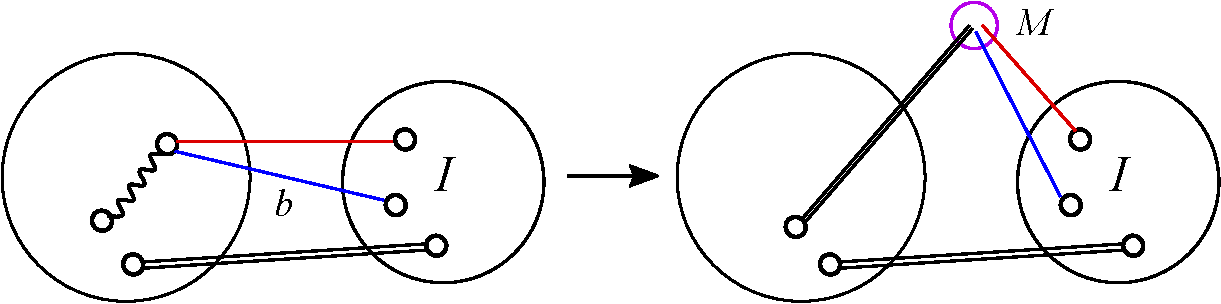
\includegraphics[width=9cm]{Isolate1.pdf}} 
\ee
In these graphs, inside the black circles are some subgraphs whose details are not drawn, and we did not indicate the directions of the solid edges for conciseness. If we replace the $T$-variable containing edge $b$ in the first graph by a graph in \eqref{Aho>2}, then we get the second graph, where the purple circle denotes a new molecule $\cal M$.  
%In the following figure, we give an example to illustrate why expanding a pivotal blue edge can break the doubly connected property. In the first graph, we draw the blue solid and $\dashed$ edges connecting an isolated sugraph $\Iso$ with its complement. The blue solid (plus $G$) edge forms a generalized $T$-variable together with a waved $S$ edge and a red solid (minus $G$) edge. Then we replace this generalized $T$-variable with a lower order $T$-expansion, and get the second graph, where $\Gamma$ is a doubly connected subgraph. 
It is easy to see that the second graph is not doubly connected anymore: in order to have a connected black net $\cal B_{black}$, we have to put the two $\dashed$ edges into $\cal B_{black}$, but then there is no edge in the blue net $\cal B_{blue}$ that connects $\cal M$ and the molecules in $\Iso$ to other molecules. 
\end{example}

 
% molecular graphs, where the vertices are molecules. Suppose in the first graph, the molecule $\cal M_2$ forms a real-isolated subgraph. Then we apply the $\Theta$ expansion \eqref{Otheta} to the pivotal blue edge, and keep the second term on the right-hand side. Then we get a new molecule $\cal M_3$ as in the second graph, whose scaling order is higher than the first graph (because of the light weight in molecule $\cal M_3$). But its naive size (without taking into account of any cancellations) can be much larger than the first graph because it is not doubly connected. To see this, we observe that after summing over $\cal M_3$, we get a single $\Theta$ edge connected with $\cal M_2$, and its sum provides a large factor of order $\eta^{-1}$. 
%%Recall that the $\Theta$ expansion \eqref{Otheta} is the second order $T$-expansion. 
%In general, if we apply the $T$-expansion \eqref{mlevelTgdef} to a blue pivotal blue edge, then replacing the edge with the higher order graphs in $\ATn$ will lead to graphs that are not doubly connected.

By definition, blue solid edges inside molecules are all redundant. Now we show that a redundant edge can be expanded without breaking the doubly connected property. 
\begin{lemma}\label{trivial_claim3}
Suppose $\cal G$ is a doubly connected graph containing a $t_{x,y_1y_2}$ variable defined in \eqref{12in4T}, where the blue solid edge $G_{\al y_1}$ is redundant. If we replace $t_{x,y_1y_2}$ with a graph on the right-hand side of \eqref{replaceT} (including any recollision, $Q$, higher order or error graph), %\hty{including any recollision, $Q$ or error graphs}, 
then the resulting graph is still doubly connected.
%{\cor Suppose a blue solid edge $b_1=G_{\al y_1}$ is redundant in $\cal G$. Moreover, suppose the ending atom $\al$ of $b_1$ is a standard neutral atom (recall Definition \ref{deflvl1}), which is connected to a waved $S$ edge $s_{x\al}$, a red solid edge $b_2=\overline G_{\al y_2}$ and (possibly) some $\times$-dotted edges. If replacing atom $\al$ and the edges attached to $\al$ with any graph in the five terms on the right-hand side of \eqref{mlevelTgdef} with $n=k$, $\fa=x$, $\fb_1=y_1$ and $\fb_2=y_2$, then the resulting graph is still doubly connected.}
\end{lemma}
\begin{proof}
We denote the blue solid edge $G_{\al y_1}$ as $b$. If we replace $t_{x,y_1y_2}$ with $ m  \Theta_{xy_1}\overline G_{y_1y_2}$ or a graph in \smash{$m (\Theta \Sdelta^{(n-1)}\Theta)_{xy_1} \overline G_{y_1y_2}$}, then it corresponds to replacing the edge $b$ with a $\dashed$ edge in the molecular graph. Obviously, this will not break the doubly connected property because a $\dashed$ edge can be also used in the blue net. Now suppose we replace $t_{x,y_1y_2}$ with a graph, say \smash{$\wt{\cal G}_{x,y_1y_2}$}, in other terms. Since $b$ is redundant, $\cal G$ has a black net $\cal B_{black}$ and a blue net $\cal B_{blue}$ satisfying Definition \ref{def 2net} such that $\cal B_{blue}\setminus\{b\}$ is still a blue net. By property (x) of Definition \ref{defn genuni}, \smash{$\wt{\cal G}_{x,y_1y_2}$} also contains a black net \smash{$\wt{\cal B}_{black}$} and a blue net \smash{$\wt{\cal B}_{blue}$} satisfying Definition \ref{def 2net}. Moreover, by property (ix) of Definition \ref{defn genuni}, the atom $x$ connects to the internal molecules of \smash{$\wt{\cal G}_{x,y_1y_2}$} through a $\dashed$ edge, say \smash{$\wt b_1$}, while the atom $y_1$ connects to the internal molecules of $\wt{\cal G}_{x,y_1y_2}$ through a blue solid or $\dashed$ or dotted edge, say $\wt b_2$. Then $\cal B_{black}\cup \wt{\cal B}_{black} \cup \{\wt b_1\}$ and $(\cal B_{blue}\setminus\{b\})\cup \wt{\cal B}_{blue} \cup \{\wt b_2\}$ are respectively the black net and blue net of the resulting graph if $\wt b_2$ is not a dotted edge. If $\wt b_2$ is a dotted edge, then the blue net can be chosen as $(\cal B_{blue}\setminus\{b\})\cup \wt{\cal B}_{blue}$ after merging the molecules connected by $\wt b_2$. In either case, the resulting graph is still doubly connected.
\end{proof}



\subsection{Pre-deterministic property} 

%Recall that after the local expansions, all the graphs are locally standard graphs, and each plus $G$ edge is  paired with a minus $G$ edge to form a generalized $T$-variable. Then we have to apply the $\Theta$ expansion \eqref{Otheta} or the $T$-expansion \eqref{mlevelTgdef} to them. 
In the proof of Theorem \ref{incomplete Texp}, we need to expand $T_{\fa, \fb_1\fb_2}$ into a sum of graphs that satisfy the properties in Definition \ref{def incompgenuni}. Hence for a graph that is not a recollision, higher order or $Q$ graph, we want its maximal subgraph to be deterministic, so that the only random parts in the graph are two plus and minus $G$ edges connected with $\oplus$ and $\ominus$. 
%For simplicity of notations, we shall call such graphs \emph{deterministic graphs}. 
On the other hand, since we want to maintain the doubly connected property during expansions, we are only allowed to expand redundant $G$ edges. Hence, not all doubly connected graphs with non-deterministic maximal subgraphs can be expanded without breaking the doubly connected property. For example, in a doubly connected graph where both the black and blue nets are trees, all the blue solid edges  between molecules are pivotal.  

Now we want to identify a graphical property with which we can tell whether a graph is potentially expanded into deterministic graphs in the end without breaking the doubly connected property. We can obtain a necessary condition by looking at the leading terms of global expansions, where we replace $t_{x,y_1y_2}$ in \eqref{12in4T} with $m \Theta_{xy_1}\overline G_{y_1y_2}$. This corresponds to changing a plus $G$ edge into a $\dashed$ edge in the molecular graph. Hence we need to be able to change all plus $G$ edges into $\dashed$ edges one by one, such that the plus $G$ edge for every expansion is redundant. This leads to the following definition. % of the \emph{pre-deterministic property}. %Later we will see that this property is also sufficient for a graph to be expanded into  deterministic graphs.

\begin{definition} [Pre-deterministic property] \label{def PDG} %  \cob details are needed. \nc
We say a doubly connected graph $\cal G$ is \emph{pre-deterministic} if the following property holds. There exists an order of all  internal blue solid edges, denoted by $b_1 \preceq b_2 \preceq \cdots$, such that for any $k$, after changing the edges $b_1, \cdots, b_{k-1} $ into $\dashed$ edges, the blue solid edge $b_k$ becomes redundant. (Recall that internal edges refer to edges that do not connect to external atoms.) We will call this order of blue solid edges a \emph{pre-deterministic order}.
\end{definition}
%Note that in the above definition, we do not care about the ``short" blue edge inside molecules. 

%\begin{remark}
%In the above definition, by removing the $\oplus$ molecule, we do not take into account the plus $G$ edge connected with $\oplus$---this edge will be handled in the last step using the cancellation property of $S_{\Delta}^{(n)}$ in \eqref{3rd_property0}. 
A pre-deterministic order is not necessarily unique. Moreover, we can always choose an order where blue solid edges inside molecules precede blue solid edges between molecules. If all internal blue solid edges in a graph $\cal G$ are redundant, then $\cal G$ is obviously a pre-deterministic graph. On the other hand, Definition \ref{def PDG} covers more general graphs. We use the following example to explain why we define pre-deterministic graphs in the above way, and why the order of blue solid edges is important: 
\begin{center}
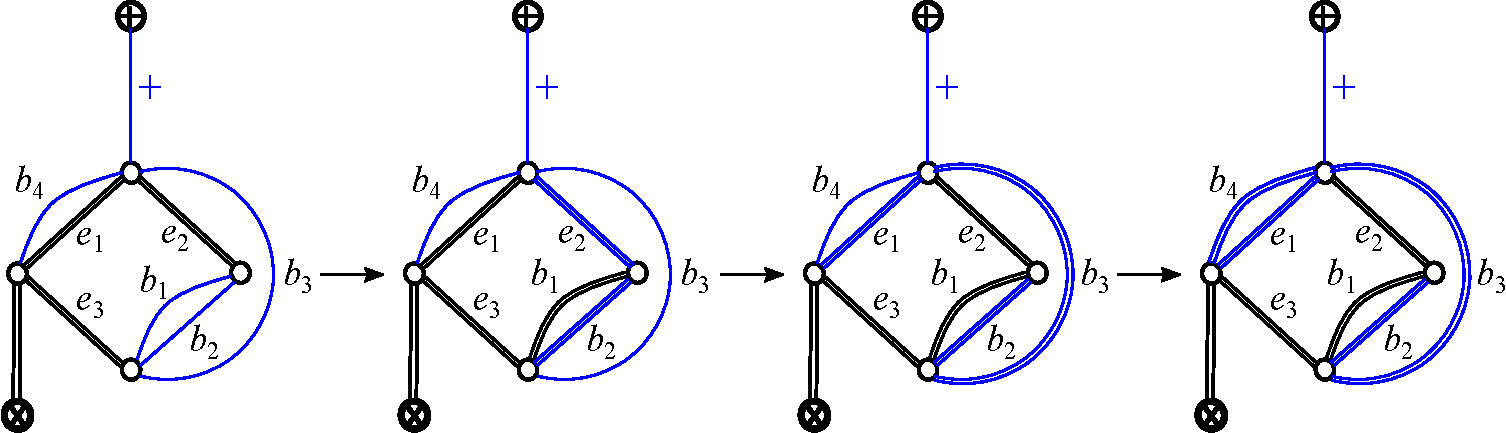
\includegraphics[width=14cm]{PDG1.pdf}
\end{center}
Here all graphs are molecular graphs without red solid edges. Note that the edges $b_1$ and $b_2$ are redundant in the first graph, but $b_3$ and $b_4$ are not. Now we show that this graph is actually pre-deterministic. First, we replace $b_1$ and $b_2$ with $\dashed$ edges. In the second graph, if we choose the black net as $\{e_1, e_3, b_1\}$ and the blue net as $\{e_2,b_2,b_3,b_4\}$, then the edge $b_3$ is redundant, and we can replace it with a $\dashed$ edge in the third graph. In the third graph, if we choose the black net as $\{e_2, e_3, b_1\}$ and the blue net as $\{e_1,b_2,b_3,b_4\}$, then $b_4$ becomes redundant, and we can replace it with a $\dashed$ edge in the fourth graph. This argument gives a pre-deterministic order $b_1\preceq b_2\preceq b_3\preceq b_4$.
%\end{remark}


%Given an isolated subgraph $\cal G_s$, it is said to be \emph{deterministic} if and only if its closure $\overline {\cal G}_s$ (recall Definition \ref{defn iso}) is deterministic. Equivalently, by a \emph{non-deterministic} isolated subgraph ${\cal G}_s$, we mean that either $\cal G_s$ contains some $G$ weights or $G$ edges, or there are plus or minus $G$ edges connecting $\cal G_s$ to its complement. Then 
\subsection{Sequentially pre-deterministic property}

Not all graphs in our expansions satisfy the pre-deterministic property. Instead, we need to consider the following extension. 

\begin{definition}[Sequentially pre-deterministic property]\label{def seqPDG}
A graph $\cal G$ is said to be sequentially pre-deterministic (SPD) if its molecular graph $\cal G_{\cal M}$ without red solid edges satisfies the following properties.
\begin{itemize}
\item[(i)] $\cal G_{\cal M}$ is doubly connected in the sense of Definition \ref{def 2net}.

\item[(ii)] Any two proper isolated subgraphs $\Iso_1$ and $\Iso_2$ satisfy either $\Iso_1\subset \Iso_2$ or $\Iso_2\subset \Iso_1$.

%$\cal G$ contains at most one chain of proper isolated subgraphs (recall Definition \ref{defn iso}), say
%\be\label{seq_iso}
%\Iso_k \subset \Iso_{k-1} \subset \cdots \subset \Iso_1 \subset  \cal G_{\max},
%\ee
%where $\Iso_{j+1}$ is a maximal isolated subgraph of $\Iso_{j}$ for any $j$. 

\item[(iii)] %The maximal subgraph $\cal G_{\max}$ or an isolated subgraph $\Iso$ of $\cal G$ is pre-deterministic if it has no proper isolated subgraph. 
The minimal isolated subgraph of $\cal G_{\cal M}$ is pre-deterministic. Moreover, given an isolated subgraph $\Iso$, if we replace its maximal isolated subgraph, say $\Iso'$, plus the two external edges with a single $\dashed$ edge, then $\Iso$ becomes pre-deterministic. (Here by ``external edges", we mean the blue solid or $\dashed$ edges connecting $\Pol(\Iso')$ to the two molecules, say $\cal M$ and $\cal M'$, in the complement of $\Pol(\Iso')$; by ``replace", we mean that we remove  $\Iso'$ and its two external edges, and add a $\dashed$ edge between $\cal M$ and $\cal M'$. If $\cal M=\cal M'$, then this $\dashed$ edge is inside $\cal M$ and will not appear in the molecular graph.) Finally, if we replace the maximal isolated subgraph of $(\cal G_{\cal M})_{\max}$ (recall that $(\cal G_{\cal M})_{\max}$ is the maximal subgraph induced on all internal molecules) plus the two external edges with a single $\dashed$ edge, then $(\cal G_{\cal M})_{\max}$ becomes pre-deterministic. 
%\hty{ We agree to explain the structure \eqref{chain_mole_sub} or \eqref{seq_iso} here or after def. then it is clearer of max subgraph}
%by using this blue edge as the first edge in the pre-deterministic order. 
\end{itemize}

\end{definition}

%\begin{remark}
Now we discuss the meanings of properties (ii) and (iii). The property (ii) means that $\cal G$ contains at most one sequence of proper isolated subgraphs, say %(recall Definition \ref{defn iso}), say
\be\label{seq_iso}
\Iso_k \subset \Iso_{k-1} \subset \cdots \subset \Iso_1 \subset  \cal G_{\max},
\ee
where $\Iso_1$ is the maximal isolated subgraph of $\cal G_{\max}$ and for any $j$, $\Iso_{j+1}$ is the maximal isolated subgraph of $\Iso_{j}$. In particular, $\cal G$ has a unique minimal isolated subgraph (namely $\Iso_k$, or $\cal G_{\max}$ if there is no proper isolated subgraph) and any subgraph has at most one maximal isolated subgraph, so property (iii) is well-defined.
%\end{remark}
Suppose %the sequence of proper isolated subgraphs in $\cal G$ is given by 
that corresponding to \eqref{seq_iso}, the sequence of proper isolated subsets of molecules is
\be\label{chain_mole}
\Pol_k \subset \Pol_{k-1} \subset \cdots \subset \Pol_1 \subset \Pol_{\max},\quad \Pol_i:= \Pol(\Iso_i), \ \ 1\le i \le k.
\ee
We draw a sequence of isolated subgraphs in the following figure, where inside each black circle is a subgraph $\Gamma_i$, which will be called a \emph{component} in our proof, and we only draw the $\dashed$ and blue solid edges between each isolated subgraph and its complement:
\be\label{chain_mole_sub}
\parbox[c]{0.7\linewidth}{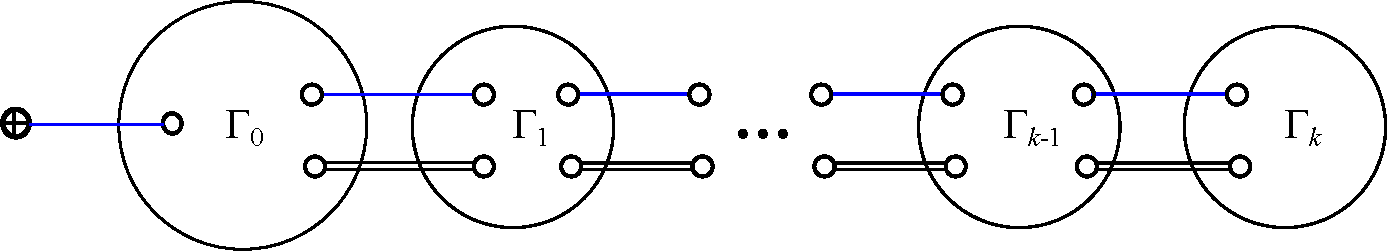
\includegraphics[width=11cm]{chain1.pdf}} 
\ee
Here for definiteness, we draw a graph with one external blue solid edge, but generally there may be zero or more than one external edges. Moreover, the blue solid edges between components can be replaced by blue $\dashed$ edges. In \eqref{chain_mole_sub}, the component $\Gamma_k$ is the minimal isolated subgraph $\Iso_k$, the component $\Gamma_{i}$, $1\le i \le k-1$, is the subgraph induced on $\Pol_{i}\setminus \Pol_{i+1}$, and $\Gamma_0$ is the subgraph induced on $\Pol_{\max}\setminus\Pol_1$. %From \eqref{chain_mole_sub}, 
One can see that the isolated subgraphs in a SPD graph form a simple chain structure. Then property (iii) means that if we replace the MIS $\Gamma_k$ and its two external edges with a $\dashed$ edge, then the resulting graph is still SPD. In the new graph, replacing the MIS $\Gamma_{k-1}$ and its two external edges with a $\dashed$ edge again gives a SPD graph. Continuing this process, after replacing $\Gamma_1$ and its two external edges with a $\dashed$ edge, $\Gamma_0$ becomes pre-deterministic. 


The reason why we define the SPD property in the above way is due to our global expansion strategy below (cf. Strategy \ref{strat_global}). We now describe one possible scenario to obtain a SPD graph. Initially, there is no proper isolated subgraph in a graph obtained from  local expansions, and its maximal subgraph is pre-deterministic. Then we find the first redundant blue solid edge in a pre-deterministic order, replace a $t$-variable containing it with a graph, say $\wt{\cal G}_1$, on the right-hand side of \eqref{replaceT}, and get a new graph $\cal G_1$. If $\wt{\cal G}_1$ contains a pre-deterministic maximal subgraph, then this subgraph becomes a pre-deterministic isolated subgraph $\Iso_1$ in graph $\cal G_1$. Next we find the first blue solid edge in a pre-deterministic order of $\Iso_1$, replace it with a graph, say $\wt{\cal G}_2$, on the right-hand side of \eqref{replaceT}, and get a new graph. Continuing this process, we get a SPD graph with a sequence of isolated subgraphs in \eqref{seq_iso}. At each step we expand the first blue solid edge in the minimal isolated subgraph. Moreover, replacing $\Iso_{i+1}$ and its two external edges with a $\dashed$ edge corresponds to replacing the first blue solid edge in a pre-deterministic order of $\Iso_{i}$ by a $\dashed$ edge, which still gives a pre-deterministic $\Iso_i$ by Definition \ref{def PDG}. This explains why we define property (iii) in such a way. 
%Then $\cal G$ is sequentially pre-deterministic if for any $1\le j \le k$,
%after replacing $I_j$ with a blue edge, then the subgraph $I_{j-1}$ becomes PDG. This explains the word ``sequential" in the name.



%As in Lemma \ref{lem localgood}, we can also show that the local expansions do not break the PDG property.

We now show that the SPD property is preserved under local expansions. 

 
\begin{lemma}\label{lem localgood2}
Let $\cal G$ be a SPD graph that satisfies the condition on external atoms in Definition \ref{def moleg}. Then applying any expansion in Definitions \ref{dot-def}, \ref{Ow-def}, \ref{multi-def}, \ref{GG-def} and \ref{GGbar-def} to $\cal G$, where the $GG$ expansion is applied as in Step 1 of Strategy \ref{strat_global} (see Lemma \ref{lem localgood}), the new graphs (including the $Q$-graphs) are all sequentially pre-deterministic.
 \end{lemma}
% \begin{remark}
%Lemma \ref{lem localgood2} is already sufficient for the purpose of this paper. However, it can be extended to the case where $\cal G$ has more than one chains of isolated subgraphs, that is, if $\cal G$ is a sequential PDG, then all the graphs from local expansions of $\cal G$ are also sequential PDG. The proof of this more general statement is almost the same as the proof for Lemma \ref{lem localgood2} below with only some minor changes in notations---the isolated subgraphs form a chain structure for $\cal G$ in Lemma \ref{lem localgood2}, while for a general sequential PDG the isolated subgraphs form a tree structure. 
% \end{remark}
 
\begin{proof}
By Lemma \ref{lem localgood}, all new graphs are still doubly connected. It remains to check the properties (ii) and (iii) in Definition \ref{def seqPDG} for any new graph, say $\wt {\cal G}$. Let $\wt{\cal G}_{\cal M}$ be its molecular graph without red solid edges.

By Lemma \ref{lvl1 lemma}, every molecule in $\wt{\cal G}$ is obtained by merging some molecules in $\cal G$. We claim that any proper isolated subset of molecules, say $\Pol$, in \smash{$\wt{\cal G}$} is obtained from merging a proper isolated subset of molecules in $\cal G$. In fact, suppose the molecules of $\Pol$ are obtained from merging a subset of molecules $\cal S$ that is not isolated in $\cal G$. Then $\cal S$ is connected to $\cal S^c$ through at least three edges, say $b_1,$ $ b_2$ and $b_3$, in the molecular graph $\cal G_{\cal M}$ without red solid edges. For $i =1,2,3 $, if $b_i$ is a $\dashed$ edge, then it is not affected in expansions and is still an external edge of $\Pol$ in $\wt{\cal G}_{\cal M}$. If $b_i$ is a plus $G$ edge in $\cal G_{\cal M}$ between molecules $\cal M_1$ and $\cal M_2$, then either $b_i$ is still a plus $G$ edge between $\cal M_1$ and $\cal M_2$ in $\wt{\cal G}_{\cal M}$, or $b_i$ becomes a connected path of two plus $G$ edges, say $b_{i,1}$ and $b_{i,2}$, between $\cal M_1$ and $\cal M_2$. %which may happen if a partial derivative $\partial_{h_{\al x}}$ or $\partial_{h_{ \beta\al}}$ acts on $b_i$. 
%(The molecules $\cal M_1$ and $\cal M_2$ may be merged with other molecules in \smash{$\wt{\cal G}_{\cal M}$}.) 
In the former case, $b_i$ is an external edge of $\Pol$ in \smash{$\wt{\cal G}_{\cal M}$}, and in the latter case, either $b_{i,1}$ or $b_{i,2}$ is an external edge of $\Pol$ in \smash{$\wt{\cal G}_{\cal M}$}. In sum, we see that $\Pol$ is connected to $\Pol^c$ through at least three edges in \smash{$\wt{\cal G}_{\cal M}$}, which contradicts the assumption that $\Pol$ is isolated. 

Now  with the above claim, we prove the property (ii) of Definition \ref{def seqPDG} for $\wt{\cal G}$. Suppose two proper isolated subsets of molecules $\Pol_1$ and $\Pol_2$ in \smash{$\wt{\cal G}$} are respectively obtained from merging two proper isolated subsets of molecules $\Pol_1'$ and $\Pol_2'$ in $\cal G$. Then we have either $\Pol_1 \subset \Pol_2$ if $ \Pol_1'\subset \Pol_2'$, or $\Pol_2 \subset \Pol_1$ if $ \Pol_2'\subset \Pol_1'$. %Hence the isolated subgraphs in $\wt{\cal G}$ form a chain.

It remains to prove the property (iii) of Definition \ref{def seqPDG} for $\wt{\cal G}$. In all expansions, it is not hard to see that
%adding a weight, or adding an edge inside a molecule, or changing an end atom of a $G$ edge to another atom in the {\bf same} molecule do not affect the sequentially pre-deterministic property because it is defined on the molecular graphs. 
there are only two types of operations that may affect the doubly connected structures:
\begin{itemize}
\item[(A)] merging a pair of molecules due to a newly added dotted or waved edge between them;

\item[(B)] replacing a plus $G$ edge $b_0$ between molecules $\cal M$ and $\cal M'$ with a path of two plus $G$ edges---edge $b$ between $\cal M$ and $\cal M''$ and edge $b'$ between $\cal M'$ and $\cal M''$---due to partial derivatives $\partial_{h_{\al x}}$ or $\partial_{h_{ \beta\al}}$, where $\cal M''$ is a different molecule from $\cal M$ and $\cal M'$.
\end{itemize}
All the other operations only act on local structures within molecules, and hence are irrelevant for our proof. In particular, the leading term of the transposed form of the $GG$ expansion gives an operation (A) merging the molecules containing $x$ and $y'$, which is the case of an internal $y$ with $y'$ in place of $y$. If $\cal O_{dot}$ turns a blue (resp.~red) solid edge between an internal atom and $\oplus$ (resp.~$\ominus$) into a dotted edge, then by Definition \ref{def moleg} this dotted edge is still a blue (resp.~red) solid edge in the molecular graph, while the identification of two internal atoms is an operation (A). When an internal atom is identified with $\otimes$ or $\oplus$ through a dotted edge, the $\dashed$ edges at this external atom are regarded as edges at the internal atom (see Definition \ref{def moleg}); this change is handled in the same way as case (v) of Lemma \ref{hard lemmQ} below. It never happens at $\ominus$, because, by the condition on external atoms in Definition \ref{def moleg}, $\ominus$ carries no $\dashed$ edge before it is identified with an internal atom. Moreover, in case (B), we have assumed that $\cal M''$ is different from $\cal M$ and $\cal M'$, because otherwise the molecular graph without red solid edges will be unchanged. To conclude the proof, it suffices to show that both operations (A) and (B) do not break the property (iii) of Definition \ref{def seqPDG}. 



Suppose the sequence of proper isolated subgraphs in $\cal G$ is given by \eqref{seq_iso} and takes the form \eqref{chain_mole_sub}. In case (A), it is easy to see that merging a pair of molecules in the same component does not break the SPD property. Now suppose we merge a pair of molecules in different components $\Gamma_{i}$ and $\Gamma_j$ with $i<j$. 
%For $l\le i$ and $i>j$, we still denote the isolated subgraph obtained from $\Iso_l$ in $\cal G$ (by merging the molecules) as $\Iso_l$ in the new graph, say $\wt{\cal G}$. 
With a slight abuse of notation, we still denote the subgraph induced on $\Pol_l$ by $\Iso_l$ in \smash{$\wt {\cal G}$}. Then the sequence of isolated subgraphs in $\wt{\cal G}$ is
$$ \Iso_k \subset \Iso_{k-1} \subset \cdots \subset \Iso_{j+1} \subset \Iso_i \subset \Iso_{i-1} \subset \cdots \subset \Iso_1. $$
In particular, $\Iso_l$ is not isolated in $\wt{\cal G}$ anymore if $j+1<l <i$. 
%\iffalse
%\be\label{eq_keepdot}
% \parbox[c]{0.5\linewidth}{\includegraphics[width=10cm]{chain1_5.png}} 
%\ee
%Here in order to have a clearer picture, we draw a dotted edge (or we can also replace it with a waved edge) between two molecules in $\Gamma_i$ and $\Gamma_j$ without merging them, but one should think of these two molecules as one single molecule (recall Definition \ref{def_poly}). Moreover, the graph component is the subgraph of $\wt{\cal G}$ induced on $\Pol_i \setminus \Pol_{j+1}$. Now in $\wt{\cal G}$,  we notice that the chain of isolated subgraphs in $\wt{\cal G}$ become
%$$ \Iso_k \subset \Iso_{k-1} \subset \cdots \subset \Iso_{j+1} \subset \Iso_i \subset \Iso_{i-1} \subset \cdots \subset \Iso_1. $$
%%where we still keep the original names of the isolated subgraphs. 
%\fi
By the SPD property of $\cal G$, we immediately obtain the following property of $\wt{\cal G}$: for $l\ge j+1$ or $l\le i-1$, if we replace $\Iso_{l+1}$ and its two external edges with a $\dashed$ edge in the molecular graph of $\wt{\cal G}$, then $\Iso_l$ becomes pre-deterministic. 
%Furthermore, it is not hard to check that $\Iso_{j+1}$ is now the maximal isolated subgraph in $\Iso_i$. (This is due to merging the two molecules in $\Gamma_i$ and $\Gamma_j$, and we omit the details of the proof.) Hence 
It remains to show that after replacing $\Iso_{j+1}$ and its two external edges with a $\dashed$ edge, the subgraph $\Iso_i$ becomes pre-deterministic. This is given by the following lemma, whose proof is postponed to Appendix \ref{sec PDG}.
%until we complete the proof of Lemma \ref{lem localgood2}. 

\begin{lemma}\label{hard lemmdot}
In the setting of \eqref{chain_mole_sub}, we merge a pair of molecules in different components $\Gamma_{i}$ and $\Gamma_j$ with $i<j$. Then after replacing $\Iso_{j+1}$ and its two external edges with a $\dashed$ edge in the molecular graph without red solid edges, the subgraph $\Iso_i$ becomes pre-deterministic. 
%If we add a dotted edge between $\Gamma_{j}$ and an external molecule ($\otimes$, $\oplus$ or $\ominus$), then after replacing $\overline I_{j+1}$ with a blue edge, the whole graph becomes pre-deterministic. 
\end{lemma}

Next we consider case (B). First, we assume that $\cal M$, $\cal M'$ and $\cal M''$ are all inside $\Gamma_i$ for some $0\le i \le k$. %Suppose the  edge $b_0$ between $\cal M$ and $\cal M'$ becomes two edges $b$ between $\cal M$ and $\cal M''$ and $b'$ between $\cal M'$ and $\cal M''$ in the new graph, say $\wt{\cal G}$. 
Then all components are unchanged after operation (B), except the component $\Gamma_i$. By definition, after replacing $\Iso_{i+1}$ and its two external edges with a $\dashed$ edge, $\Iso_i$ becomes pre-deterministic in $\cal G$, and suppose a pre-deterministic order of $\Iso_i$ is $e_1 \preceq \cdots \preceq e_{\ell-1} \preceq b_0 \preceq e_{\ell+1} \preceq \cdots$. Then in \smash{$\wt{\cal G}$}, after replacing $\Iso_{i+1}$ and its two external edges with a $\dashed$ edge, $e_1\preceq \cdots\preceq e_{\ell-1}\preceq b\preceq b' \preceq  e_{\ell+1}\preceq\cdots$ is a pre-deterministic order in $\Iso_i$. Using this fact, we can readily check that $\wt{\cal G}$ is still SPD.

Second, we assume that $\cal M\in \Gamma_i$, $\cal M'\in \Gamma_{i+1}$ and (1) $\cal M''\in \Gamma_i$, or (2) $\cal M''\in \Gamma_{i+1}$. Suppose we have replaced $\Iso_{i+2}$ and its two external edges with a $\dashed$ edge in $\Iso_{i+1}$ and get the following graphs:
\begin{center}
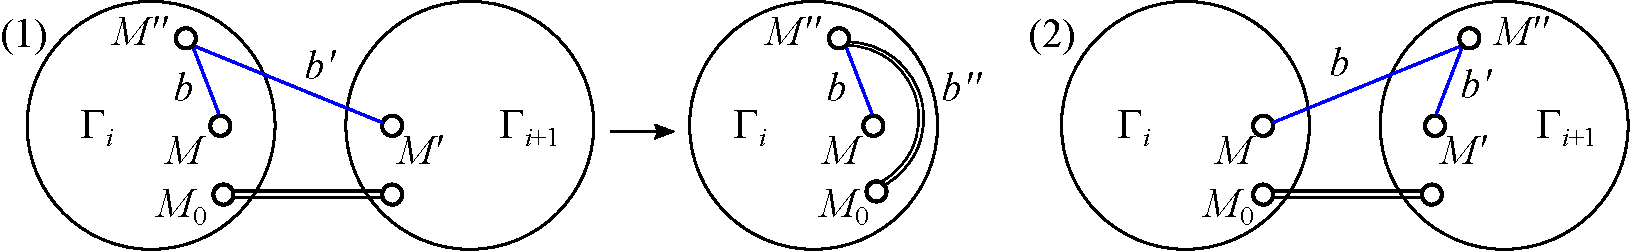
\includegraphics[width=13cm]{M123.pdf}
\end{center}

In case (1), $\Iso_{i+1}$ is pre-deterministic because it is unchanged after the operation (B). In the second graph, we replace $\Iso_{i+1}$ and its two external edges with a $\dashed$ edge $b''$. We show that the edge $b$ is now redundant in $\Iso_{i}$. By the  doubly connected property of $\cal G$, removing the subgraph $\Iso_{i+1}$ and its two external edges still gives a doubly connected graph. Correspondingly, in the first graph of case (1), if we remove $\Gamma_i$, its two external edges and edge $b$, we still get a doubly connected graph. Hence the edge $b$ is redundant in the second graph of case (1). Now if we replace $b$ with a $\dashed$ edge, then the path of $\dashed$ edges $b''$ and $b$ will play the role of a single $\dashed$ edge between $\cal M_0$ and $\cal M$ in $\Iso_i$, and hence $\Iso_{i}$ becomes pre-deterministic by the property (iii) of Definition \ref{def seqPDG} for the original graph $\cal G$.

In case (2), $\Iso_{i+1}$ is still pre-deterministic by choosing the edge $b'$ as the last edge in a pre-deterministic order. Moreover, after replacing $\Iso_{i+1}$ and its two external edges with a $\dashed$ edge, $\Iso_{i+1}$ becomes pre-deterministic by the property (iii) of Definition \ref{def seqPDG} for the original graph $\cal G$. %Hence we observe that in both cases, $\wt {\cal G}$ obtained from operation (B) is pre-deterministic.

It remains to consider the case where $\cal M''$ is in a different component from both $\cal M$ and $\cal M'$. %Depending on the relations between $\cal M$ and $\cal M'$, we have five different cases as given by the following lemma. 



\begin{lemma}\label{hard lemmQ}
In the setting of \eqref{chain_mole_sub}, suppose a blue solid edge between molecules $\cal M$ and $\cal M'$ (possibly $\cal M=\cal M'$, in which case the edge is inside $\cal M$) is replaced by a path of two blue solid edges from $\cal M$ to $\cal M''$ and from $\cal M''$ to $\cal M'$. Let the new graph be \smash{$\wt{\cal G}$}, and with a slight abuse of notation, we still denote the subgraphs induced on $\Pol_l$ by $\Iso_l$ in $\wt {\cal G}$. Suppose $\cal M''$ is inside component $\Gamma_j$.  Then we have the following five cases for the molecular graph $\wt {\cal G}_{\cal M}$ without red solid edges.
\begin{itemize}
\item[(i)] If $\cal M,\cal M' \in \Gamma_i$ and $i<j$, then $\Iso_{j+1}$ is the maximal isolated subgraph of $\Iso_i$. Moreover, after replacing $\Iso_{j+1}$ and its two external edges with a $\dashed$ edge, the subgraph $\Iso_i$ becomes pre-deterministic.
 
\item[(ii)] If $\cal M,\cal M' \in \Gamma_i$ and $i>j$, then $\Iso_{i+1}$ is the maximal isolated subgraph of $\Iso_j$. Moreover, after replacing $\Iso_{i+1}$ and its two external edges with a $\dashed$ edge, the subgraph $\Iso_j$ becomes pre-deterministic.
 
 \item[(iii)] If $\cal M\in \Gamma_i$, $\cal M'\in \Gamma_{i+1}$ and $i<j$, then $\Iso_{i+1}$ is the maximal isolated subgraph of $\Iso_i$, and $\Iso_{j+1}$ is the maximal isolated subgraph of $\Iso_{i+1}$. Moreover, after replacing $\Iso_{j+1}$ and its two external edges with a $\dashed$ edge, the subgraph $\Iso_{i+1}$ becomes pre-deterministic.
 
 \item[(iv)] If $\cal M\in \Gamma_i$, $\cal M'\in \Gamma_{i+1}$ and $i>j$, then $\Iso_{i+1}$ is the maximal isolated subgraph of $\Iso_j$. Moreover, after replacing $\Iso_{i+1}$ and its two external edges with a $\dashed$ edge, the subgraph $\Iso_{j}$ becomes pre-deterministic.

\item[(v)] If $\cal M$ is an external molecule and $\cal M'\in \Gamma_0$, then $\Iso_{j+1}$ is the maximal proper isolated subgraph. Moreover, after replacing $\Iso_{j+1}$ and its two external edges with a $\dashed$ edge, the maximal subgraph \smash{$\wt{\cal G}_{\max}$} becomes pre-deterministic.
\end{itemize}
%After adding $Q$-pulled between two polymers, then all the polymers between these two polymers (on the original polymer tree) become locally potential grey.  
\end{lemma}

%Then we have five different cases as in the following figure: 
%\begin{center}
%	\includegraphics[width=16cm]{Five_cases.png}
%\end{center}
%where we only draw the relevant $\Gamma$ components, while all the other ones are unchanged. For these five cases, we have the following lemma, whose proof will be given in Appendix \ref{sec PDG}. 

The proof of Lemma \ref{hard lemmQ} will be postponed to Appendix \ref{sec PDG}. Similar to case (A), combining Lemma \ref{hard lemmQ} with the SPD property of the original graph $\cal G$, we can readily show that the new graph obtained from the operation (B) is still SPD. We omit the details. This concludes Lemma \ref{lem localgood2}.
%Finally, we can conclude Lemma \ref{hard lemma} with Lemma \ref{keykeykey}. If we have two polymers connected through $Q$-pulled edges at some step of expansions, then the molecules between them will combine into a polymer that is locally potential grey. Hence even in the case $\dag$, the ``big" MIFT we finally get will be PDG.
 \end{proof}
Similar to Lemma \ref{lem localgood2}, we have the following result for $Q$-expansions.   
%I suggest to add this following lemma, since this property are very useful in the whole expansion. 

\begin{lemma}\label{lem localgoodQ}
Let $\cal G_0$ in \eqref{QG} be a SPD graph that satisfies the condition on external atoms in Definition \ref{def moleg}. Then applying the $Q$-expansions in Section \ref{sec defnQ}, the new graphs (including the $Q$-graphs) are all SPD.
\end{lemma}
\begin{proof}
The proof of this lemma is similar to the one for Lemma \ref{lem localgood2} by using Lemmas \ref{hard lemmdot} and \ref{hard lemmQ}, because $Q$-expansions are also local expansions as those in Lemma \ref{lem localgood2}. More precisely, the operations in Steps 1--3 of Section \ref{sec defnQ} that may affect the molecular graph without red solid edges are the operations (A) and (B) in the proof of Lemma \ref{lem localgood2}, the identifications of atoms through dotted edges, and the replacement of a weight $G_{aa}$ on an atom $a\ne x$ by $G_{ax}G_{xa}(G_{xx})^{-1}$ through \eqref{resol_exp0}; the last one is an operation (B) for a blue solid edge inside the molecule containing $a$, i.e., Lemma \ref{hard lemmQ} with $\cal M=\cal M'$. The colours of the dotted edges at $\oplus$ and $\ominus$ are as in the proof of Lemma \ref{lem localgood2}, because in our graphs $\fb_1$ only appears as the second index of $G$ entries and $\fb_2$ only as the second index of $\overline G$ entries. As in that proof, case (v) of Lemma \ref{hard lemmQ} is used only for the $\dashed$ edges at a newly identified $\otimes$ or $\oplus$, and never at $\ominus$. We omit the other details.
\end{proof}



\section{Proof of Theorem \ref{incomplete Texp} and Corollary \ref{lem completeTexp}}\label{sec global}


%For this purpose, we introduce the concept of globally standard graphs. In each globally standard graph, there is a canonical order of all the $T$-variables. Then roughly speaking, the core reason why our global expansion strategy works is that every globally standard graph can be expanded, while each expansion of a globally standard graph still gives globally standard graphs as long as we expand the {\bf first} $T$-variable in it.  

\subsection{Proof of Corollary \ref{lem completeTexp}}\label{sec lastglobal}

Given the $n$-th order $\incomp$ constructed in Theorem \ref{incomplete Texp}, we can solve \eqref{mlevelT incomplete} to get that
\begin{align}
	T_{\fa,\fb_1\fb_2} &=  m \left( \frac{1}{1-\Theta \wtSdelta^{(n)}}\Theta\right)_{\fa\fb_1} \overline G_{\fb_1\fb_2} \nonumber \\
	&   + \sum_x \left( \frac{1}{1-\Theta \wtSdelta^{(n)}}\right)_{\fa x} \left[  (\PIT^{(n)})_{x,\fb_1 \fb_2} + (\AITn)_{x,\fb_1 \fb_2} + (\QITn)_{x,\fb_1 \fb_2}+ (\Err'_{n,D})_{x,\fb_1\fb_2} \right] . \label{solving_T}
\end{align}	
By the property (iv) of Definition \ref{def incompgenuni}, we can write that 
$$(\PIT^{(n)})_{x,\fb_1 \fb_2} = \sum_y \Theta_{xy} (\cal G_R^{(n)})_{y,\fb_1 \fb_2},\quad (\AITn)_{x,\fb_1 \fb_2} = \sum_y \Theta_{xy}(\cal G_A^{(>n)})_{y,\fb_1 \fb_2} ,$$
$$ (\QITn)_{x,\fb_1 \fb_2}= \sum_y \Theta_{xy}(\cal G_Q^{(n)})_{y,\fb_1 \fb_2},\quad (\Err'_{n,D})_{x,\fb_1\fb_2}=\sum_y \Theta_{xy}(\cal G_{err}^{(n,D)})_{y,\fb_1 \fb_2} ,$$
for some sums of graphs $\cal G_R^{(n)}$, $\cal G_A^{(>n)}$, $\cal G_Q^{(n)}$ and $\cal G_{err}^{(n,D)}$. Using the definition \eqref{theta_renormal}, we can write \eqref{solving_T} as 
\begin{align}
  T_{\fa,\fb_1\fb_2} &=  m \Theta^{(n)}_{\fa\fb_1} \overline G_{\fb_1\fb_2}   + \sum_x \Theta^{(n)}_{\fa x} \left[(\cal G_R^{(n)})_{x,\fb_1 \fb_2} + (\cal G_A^{(>n)})_{x,\fb_1 \fb_2}+  (\cal G_Q^{(n)})_{x,\fb_1 \fb_2} +   (\cal G_{err}^{(n,D)})_{x,\fb_1 \fb_2}\right] . \label{solving_T2}
\end{align}	
We expand $\Theta^{(n)}$ as 
\be\label{expand_thetan}
\Theta^{(n)}= \sum_{k=0}^D ( \Theta \wtSdelta^{(n)})^{k}\Theta + \Theta^{(n)}_{err},\quad \Theta^{(n)}_{err}:= \sum_{k>D} ( \Theta \wtSdelta^{(n)})^{k}\Theta.
\ee
The terms $( \Theta \wtSdelta^{(n)})^{k}\Theta$ can be expanded into sums of labelled $\dashed$ edges, and we regard  \smash{$(\Theta^{(n)}_{err})_{xy}$} as a new type of $\dashed$ edge of scaling order $\ge 2(D+2)$ between atoms $x$ and $y$. Then we plug the expansion \eqref{expand_thetan} into \eqref{solving_T2} and rearrange the resulting graphs as follows. First, all graphs containing \smash{$\Theta^{(n)}_{err}$} and graphs from \smash{$\sum_x \Theta^{(n)}_{\fa x} (\cal G_{err}^{(n,D)})_{x,\fb_1 \fb_2}$} will be included into $(\Err_{n,D})_{\fa,\fb_1\fb_2}$. For other graphs, 
\begin{itemize}
\item the term \smash{$m \Theta^{(n)}_{\fa\fb_1} \overline G_{\fb_1\fb_2}$} will give the first two terms on the right-hand side of \eqref{mlevelTgdef} and some higher order graphs in $ (\ATn)_{\fa,\fb_1\fb_2}$; the latter are of the form $m\Theta'_{\fa\fb_1}\overline G_{\fb_1\fb_2}$ with a labelled $\dashed$ edge $\Theta'$, and we write them as normal regular graphs using $\cal O_{dot}$, i.e. $\overline G_{\fb_1\fb_2}=\mathbf 1_{\fb_1=\fb_2}\overline G_{\fb_1\fb_1}+\mathbf 1_{\fb_1\ne\fb_2}\overline G_{\fb_1\fb_2}$. These are the only graphs in $(\ATn)_{\fa,\fb_1\fb_2}$ without internal atoms;

\item the term \smash{$\sum_x \Theta^{(n)}_{\fa x} (\cal G_R^{(n)})_{x,\fb_1 \fb_2}$} will give $(\PTn)_{\fa,\fb_1\fb_2}$ and some higher order graphs in $ (\ATn)_{\fa,\fb_1\fb_2}$;  

\item the term \smash{$\sum_x \Theta^{(n)}_{\fa x} (\cal G_A^{(>n)})_{x,\fb_1 \fb_2}$} will give higher order graphs in $ (\ATn)_{\fa,\fb_1\fb_2}$;  

\item the term \smash{$\sum_x \Theta^{(n)}_{\fa x} (\cal G_Q^{(n)})_{x,\fb_1 \fb_2}$} will give graphs in $(\QTn)_{\fa,\fb_1\fb_2}$. 
\end{itemize}
This concludes Corollary \ref{lem completeTexp}. 




\subsection{Globally standard graphs}\label{sec_global_standard}

For the rest of this section, we focus on proving Theorem \ref{incomplete Texp}. In this subsection, we introduce the concept of \emph{globally standard graphs}. By taking into account the external red solid edges connected with isolated subgraphs, we define the following concept of weakly and strongly isolated subgraphs.

\begin{definition}[Weakly and strongly isolated subgraphs]\label{def_weakstrong}
%By taking into account the minus $G$ edges (red solid edges), 
%We divide the isolated subgraphs into the following two types.
%\begin{itemize}
%\item 
An isolated subset of molecules $\Pol$ is said to be \emph{strongly isolated} if there is \emph{at most one} red solid edge between $\Pol$ and $\Pol^c$, and the subgraph $\Iso_\Pol$ induced on $\Pol$ is called a strongly isolated subgraph. % only through three edges: an edge in the black net, an edge in the blue net, and a red solid edge.
Otherwise, $\Pol$ and $\Iso_\Pol$ are said to be weakly isolated (i.e. a weakly isolated subgraph is an isolated subgraph that is not 
strongly isolated). 


%\item An isolated subset of molecules $\Pol$ is said to be {\bf weakly isolated} if there is at least two red solid edges between $\Pol$ and $\Pol^c$. The corresponding subgraph $\Iso(\Pol)$ is called a weakly isolated subgraph.

%An isolated subgraph $\cal G_s$ is said to be {\bf pseudo-isolated} if $\cal G_s$ is connected with its complement through an edge in the black net, an edge in the blue net, and more than one red solid edges.
%\end{itemize}
\end{definition}

%----------heruristic discussion
%In the following figure, $\Iso$ is a strongly (resp. weakly) isolated subgraph in the first (resp. second) graph. In the first graph, if $\Iso$ contains no solid blue edges, then $\Iso$ is connected with a pair of red and blue external solid edges. Moreover, we cannot expand them without breaking the doubly connected property because the solid blue edge is pivotal. In the second graph, if $\Iso$ contains no solid blue edges, then it must contain an atom which is connected with more red solid edges than blue solid edges. Hence we can expand the graph by performing a local expansion $\cal O_{multi}$ (recall Definition \ref{multi-def}) or $\cal O_{GG}$ (recall Definition \ref{GG-def}). 
%If the graph $\Iso$ is still isolated in the expansion, then the number of its external red solid edges is $\ge 2$, and we can always perform a local expansion because the red edges and blue solid edges do not match. Such local expansions only stop when $\Iso$ is not isolated anymore due to newly added waved, dotted or blue solid edge between $\Iso$ and its complement. Lemma \ref{lem localgood2} tells that the resulting graph is still SPD, and we can continue performing the global expansions.
%
%\begin{center}
%\includegraphics[width=12cm]{Weak_strong.png}
%\end{center}
%------------------------------

With Definition \ref{def seqPDG} and Definition \ref{def_weakstrong}, we define globally standard graphs.

\begin{definition}[Globally standard graphs]\label{defn gs}
A graph is said to be \emph{globally standard} if it is SPD, and every proper isolated subgraph of it is weakly isolated. 
\end{definition}

%\hty{ we need to say a few words why this is important.} 

The reason for introducing globally standard graphs is to avoid \emph{non-expandable graphs}, i.e. graphs that cannot be expanded without breaking the doubly connected property. As an example, we consider the following two graphs, where $\Gamma_1$ is strongly isolated in (a) and weakly isolated in (b):
\begin{center}
	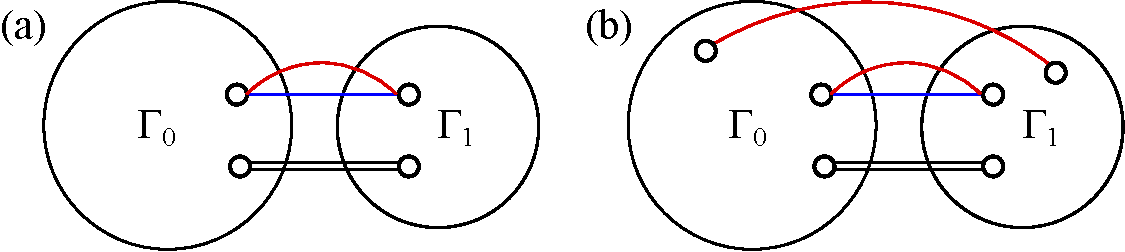
\includegraphics[width=9cm]{Weak_iso.pdf}
\end{center}
Suppose both graphs (a) and (b) are SPD with $\Gamma_1$ being the minimal isolated subgraph. If $\Gamma_1$ contains blue solid edges, then we can either perform local expansions or expand the first blue solid edge in a pre-deterministic order of $\Gamma_1$. Now suppose $\Gamma_1$ does not contain any internal blue solid edge, then it is not locally standard in graph (b) because there are more external red solid edges than blue solid edges. Hence we can perform local expansions to graph (b). On the other hand, if both $\Gamma_0$ and $\Gamma_1$ in (a) are deterministic, then graph (a) is locally standard and only contains a pivotal blue solid edge, so it cannot be expanded without breaking the doubly connected property. Such a graph may not be included into one of the six terms on the right-hand side of \eqref{mlevelT incomplete}. 
% may not be included into any term on the right-hand side of \eqref{mlevelT incomplete} if it is not a recollision, $Q$, higher order or error graph. 
In sum, the SPD property in Definition \ref{defn gs} gives a canonical order of blue solid edges to expand, while the weakly isolated property guarantees that our expansions will not give non-expandable graphs. %graphs which only contain pivotal blue solid edges.  

%Before discussing the global expansions, we first 

Now we state some additional properties satisfied by the graphs in the $T$-expansion and $\incomp$. Recall the definition of minimal isolated subgraphs (MIS) in Definition \ref{defn_min_iso}, and condition (E) on the external atoms in Definition \ref{def moleg}. We say that a graph has the \emph{charge pattern} if $\oplus$ appears only as the second index of blue solid edges $G_{u\fb_1}$, $\ominus$ appears only as the second index of red solid edges $\overline G_{u\fb_2}$, and every waved edge connects two internal atoms; here, if an external atom is connected with an internal atom through a dotted edge, then the edges at this external atom are regarded as edges at the internal atom.

\begin{definition} [$T$-expansion and $\incomp$: additional properties]\label{def genuni2}
%An $n$-th order $T$-expansion of $T_{\fa,\fb_1 \fb_2}$ is an expression satisfying 
The graphs in Definition \ref{defn genuni} satisfy the following additional properties. 

\begin{enumerate}

\item Every graph in $(\PTn)_{\fa,\fb_1\fb_2}$ is globally standard, satisfies condition (E) and has the charge pattern. %, and all the non-standard neutral atoms (recall Definition \ref{def SNA}) in it belong to the MIS.

\item Every graph in $  (\ATn)_{\fa,\fb_1\fb_2} $ is SPD. %, and all the non-standard neutral atoms in it belong to the MIS.
If it has an internal atom, then it satisfies condition (E) and has the charge pattern; otherwise, every $\dashed$ edge at $\otimes$ ends at $\oplus$. Moreover, every $\oplus$/$\ominus$-recollision graph in $(\ATn)_{\fa,\fb_1\fb_2}$ is globally standard.


\item Every $Q$-graph in $(\QTn)_{\fa,\fb_1\fb_2} $ is SPD. % and all the non-standard neutral atoms in it belong to the MIS.
Moreover, the atom in the $Q$-label of a $Q$-graph belongs to the MIS, i.e. all solid edges and weights have the same $Q$-label $Q_x$ for an atom $x$ inside the MIS, except in the following two cases: $x$ is $\oplus$ or $\ominus$ and is connected with an atom in the MIS through a waved edge; or the $Q$-graph has no internal atoms, in which case $x=\oplus$ and every $\dashed$ edge at $\otimes$ ends at $\oplus$. A $Q$-graph with an internal atom satisfies condition (E) and has the charge pattern.

\item If $\oplus$ and $\ominus$ are connected by a path of dotted edges in a graph in $(\PTn)_{\fa,\fb_1\fb_2}$ or $(\ATn)_{\fa,\fb_1\fb_2}$ (resp. in a $Q$-graph in $(\QTn)_{\fa,\fb_1\fb_2}$), then this graph has scaling order $\ge 5$ (resp. $\ge 4$).

\end{enumerate}
$(\PITn)_{\fa,\fb_1 \fb_2}$, $(\AITn)_{\fa,\fb_1\fb_2}$, $ (\QITn)_{\fa,\fb_1\fb_2}  $ and $(\Err'_{n,D})_{\fa,\fb_1\fb_2}$ in Definition \ref{def incompgenuni} also satisfy these properties.
\end{definition}


By this definition, the higher order and $Q$ graphs in the $T$-expansion and $\incomp$ may contain strongly isolated subgraphs, but the recollision graphs do not. The heuristic reason is as follows. We only expand globally standard graphs, and we want to show that an expansion of a globally standard graph still gives globally standard graphs plus some graphs that are not needed to be expanded further (i.e. recollision, $Q$, higher order and error graphs). Suppose we substitute a $t$-variable with a recollision graph $\cal G$ in \smash{$\PT^{(n-1)}$}. In order for the resulting graph to be globally standard, $\cal G$ cannot contain any strongly isolated subgraph. %\hty{ add This explains why recollision graphs have to be weakly isolated.}  
This explains why recollision graphs have to be weakly isolated. If we substitute a $T$-variable with a graph in \smash{$\AT^{(n-1)}$}, then the resulting graph will be of scaling order $>n$ and we will not expand this graph further. Hence we do not require this graph to be globally standard. Finally, if we substitute a $T$-variable with a $Q$-graph $\cal G$ in \smash{$\QT^{(n-1)}$} and get a graph, say $\cal G_0$, then we need to perform $Q$-expansions to $\cal G_0$. Suppose a $Q$-expansion of $\cal G_0$ is given by \eqref{G0Q}. By the property (iv) of Lemma \ref{Q_lemma}, there will be solid edges connecting the atom in the $Q$-label of $\cal G$, say $x$, to old atoms in the original graph. Since $x$ belongs to the MIS of $\cal G$, one can see that the strongly isolated subgraphs in $\cal G_0$ before the $Q$-expansion are not strongly isolated anymore in graphs $\cal G_\omega$ after the $Q$-expansion. The rigorous argument will be given in the proof of Lemma \ref{lem globalgood} below.


With Lemma \ref{lem localgood2}, we can easily show that local expansions preserve the globally standard property. % in Definition \ref{def genuni2}. %More precisely, we have the following lemma.


\begin{lemma}\label{lem localgood3}
Let $\cal G$ be a globally standard graph without any $P/Q$ labels that satisfies condition (E).
\begin{enumerate}
\item Apply any expansion in Definitions \ref{dot-def}, \ref{Ow-def}, \ref{multi-def}, \ref{GG-def} and \ref{GGbar-def} to $\cal G$, where the $GG$ expansions are applied as in Step 1 of Strategy \ref{strat_global} below (i.e. the waved edge in the main term of \eqref{Oe2x} connects $x$ with an internal atom). The new graphs (including the $Q$-graphs) are all globally standard.

\item Apply any expansion in Definitions \ref{Ow-def}, \ref{multi-def}, \ref{GG-def} and \ref{GGbar-def} on an atom in the MIS of $\cal G$. In each new $Q$-graph, the atom in the $Q$-label also belongs to the MIS. %minimal isolated subgraph.

%Suppose the non-standard neutral atoms all belong to the MIS of $\cal G$. Then applying any expansion in Definitions \ref{Ow-def}, \ref{multi-def}, \ref{GG-def} and \ref{GGbar-def} on a non-standard neutral atom $x$ of $\cal G$, all the non-standard neutral atoms also belong to the MIS in each new graph. Moreover, in each new $Q$-graph, the atom in the $Q$-label belongs to the MIS.
\end{enumerate}
\end{lemma}
\begin{proof}
By Lemma \ref{lem localgood2}, the new graphs are all SPD (for the transposed form of $\cal O_{GG}^{(x)}$, the arguments are those for the case where $y$ is internal, with $y'$ in place of $y$). Let $\wt{\cal G}$ be one of the new graphs. As shown in the proof of Lemma \ref{lem localgood2}, any proper isolated subset of molecules $\Pol$ in $\wt{\cal G}$ is obtained from merging a proper isolated subset of molecules, say $\Pol_0$, in $\cal G$. Moreover, it easy to see that the number of external red solid edges of $\Pol$ in $\wt{\cal G}$ is larger than or equal to the number of external red solid edges of $\Pol_0$ in ${\cal G}$. Since $\Pol_0$ is weakly isolated in ${\cal G}$, we get that $\Pol$ is also weakly isolated in $\wt{\cal G}$. This concludes (i). 
The property (ii) can be checked readily using the Definitions \ref{Ow-def}, \ref{multi-def}, \ref{GG-def} and \ref{GGbar-def}.
%\iffalse
%For (ii), %recall that the expansions in Definitions \ref{Ow-def}, \ref{multi-def}, \ref{GG-def} and \ref{GGbar-def} only act on non-standard neutral atoms. In particular, 
%on the one hand, a non-standard neutral atom $x_0$ in $\cal G$ belongs to the MIS. Then it is easy to check with Definitions \ref{Ow-def}, \ref{multi-def}, \ref{GG-def} and \ref{GGbar-def} that $x_0$ is still in the MIS after the expansion. On the other hand, notice that a standard neutral atom $x_1$ in $\cal G$ remains to be standard neutral in every new graph, unless it is identified with another atom, say $y_1$, through an dotted edge. This only occurs when $x_1$ is connected with $y_1$ through a newly appeared $G$ edge, and we have added a dotted edge between them when applying $\cal O_{dot}$. From Definitions \ref{Ow-def}, \ref{multi-def}, \ref{GG-def} and \ref{GGbar-def}, we see that atom $y_1$ must be in a molecule that contains a non-standard neutral atom, say $y_0$, in $\cal G$. By assumption, $y_0$ belongs to the MIS of $\cal G$. Hence after identifying $x_1$ with $y_1$, we can check that atom $x_1$ must also belong to the MIS of the new graph. 
%
%Finally, we notice that the atom in the $Q$-label of a $Q$-graph, say $x$, belongs to a molecule around an atom that is originally not standard neutral in $\cal G$. With this fact, we can get that the atom $x$ also belongs to the minimal isolated subgraph in the new graph. \fi 
\end{proof}

 
The following lemma is key to our proof. Roughly speaking, it shows that the globally standard property is preserved if we expand the \emph{first} blue solid edge in a pre-deterministic order of the MIS. 

%The above lemma shows that the local expansions preserve the local standard property of graphs. Later we will show that the global standard property will be preserved as long as we expand the {\bf first} blue solid edge in the pre-deterministic order of the minimal isolated subgraph at each step. Then roughly speaking, the core argument of our proof is to show that every globally standard graph can be expanded, while each expansion of a globally standard graph still gives globally standard graphs. % as long as we expand the {\bf first} $T$-variable in it.


\begin{lemma}\label{lem globalgood}
Suppose $\cal G$ is a globally standard graph without $P/Q$ labels, which is not a $\oplus$/$\ominus$-recollision graph, satisfies condition (E), has the charge pattern, has only $\dashed$ edges at $\otimes$, and has scaling order $\ge 4$. Let $\Iso_k$ be the MIS of $\cal G$, and suppose that $\Iso_k$ is locally standard. Consider a $t_{x,y_1y_2}$ variable in $\cal G$ defined by \eqref{12in4T}, so that the blue solid edge $G_{\al y_1}$ is %either inside a molecule in $\Iso_k$, or is
the first blue solid edge in a pre-deterministic order of $\Iso_k$, and $y_2$ is an internal atom. In (1)--(5) below, every graph obtained from a replacement is written as a sum of normal regular graphs using $\cal O_{dot}$, and its scaling order is that of these normal regular graphs (recall Definition \ref{def scaling}). We let $\epsilon=1$ if $y_1=y_2$ and $\oplus$, $\ominus$ are connected by a path of dotted edges in the graph that replaces $t_{x,y_1y_2}$, and $\epsilon=0$ otherwise.
The same statements hold for a $t_{y_1y_2,x}$ variable such that $G_{y_1\al}$ is the first blue solid edge in a pre-deterministic order of $\Iso_k$ and $y_2$ is an internal atom, where we use the expansion of $t_{y_1y_2,x}$ obtained by taking transpositions of all $G$ entries in \eqref{replaceT}.
  
%Let $b_1$ be the first plus $G$ edge in a pre-deterministic order of $\Iso_k$. Suppose this plus edge is $G_{\al y_1}$ in the $t_{x,y_1y_2}$ variable in \eqref{12in4T}. 
%Then for any $l$-th order $T$-expansion with $l\le n-1$, 

\begin{itemize}
\item[(1)] If we replace $t_{x,y_1y_2}$ with a graph in the first two terms on the right-hand side of \eqref{replaceT},
%$\overline m^{-1}\Theta_{xy_1}\overline G_{y_1y_2}$ or a labelled $\dashed$ $\Theta$ edge $\overline m^{-1}(\Theta \Sele_{2k_1}\Theta  \Sele_{2k_2}\Theta \cdots \Theta  \Sele_{2k_l}\Theta)_{xy_1}\overline G_{y_1y_2}$, 
then the resulting graph, say \smash{$\wt{\cal G}$}, has no $P/Q$ labels and is globally standard. % and has a MIS containing all  non-standard neutral atoms. 
Moreover, \smash{$\wt{\cal G}$} either has a strictly higher scaling order than $\cal G$, or is obtained by replacing $t_{x,y_1y_2}$ with $ m\Theta_{xy_1}\overline G_{y_1y_2}$.

\item[(2)] If we replace $t_{x,y_1y_2}$ with a graph $(\cal G_{R})_{x,y_1 y_2}$ in $(\wtPT^{(n-1)})_{x,y_1 y_2}$, then the resulting graph has no $P/Q$ labels, is globally standard and has a scaling order $\ge \ord(\cal G) +1 $, except in the following case: if $y_1=y_2$ and $(\cal G_{R})_{x,y_1 y_2}$ comes from the term with $\mathbf 1_{\al = y_1}\mathbf 1_{\al = y_2}$ in the definition of $\wtPT^{(n-1)}$ (see the display above \eqref{replaceT}), then the resulting graph has the same scaling order as $\cal G$ and two fewer solid edges (one blue and one red). % and has a MIS containing all non-standard neutral atoms.

\item[(3)] If we replace $t_{x,y_1y_2}$ with a graph $(\cal G_{A})_{x,y_1y_2}$ in $(\AT^{(>n-1)})_{x,y_1 y_2}$, then the resulting graph  has no $P/Q$ labels, is SPD and has a scaling order $\ge \ord(\cal G)+n-2-2\epsilon$. If $\epsilon=1$, then the resulting graph is moreover globally standard and has a scaling order $\ge \ord(\cal G)+1$. % and has a MIS containing all non-standard neutral atoms.

\item[(4)] Suppose we replace $t_{x,y_1y_2}$ with a graph $(\cal G_{Q})_{x,y_1y_2}$ in $(\QT^{(n-1)})_{x,y_1 y_2}$ and get a graph $\wt{ \cal G} $. Then applying $\cal O_{dot}$ and the $Q$-expansions in Section \ref{sec defnQ} (with the properties in Lemma \ref{Q_lemma}), we can expand it into a sum of $\OO(1)$ many graphs: %for any fixed $D>0$,
\be\label{mlevelTgdef3_Q}
\wt{ \cal G} = \sum_\omega \cal G_\omega  + \cal Q   + \cal G_{err} ,
\ee
where every $\cal G_\omega$ has no $P/Q$ labels, is globally standard and has a scaling order $\ge \ord(\cal G) +1 $; %and has a MIS containing all non-standard neutral atoms; 
$\cal Q$ is a sum of $Q$-graphs, each of which is SPD and has a MIS containing the atom in the $Q$-label; 
%and each of them whose each of which is  and has a minimal isolated subgraph containing all non-standard neutral atoms and the atom in the $Q$-label; 
$\cal G_{err}$ is a sum of doubly connected graphs of scaling orders $> D$.

\item[(5)] If we replace $t_{x,y_1y_2}$ with a graph $(\cal G_{err})_{x,y_1y_2}$ in $(\Err_{n-1,D})_{x,y_1 y_2}$, then the resulting graph is doubly connected and has a scaling order $\ge \ord(\cal G)+D-1-2\epsilon> D$.
\end{itemize}
\end{lemma}
\begin{proof}
We first record how the scaling order changes in a replacement. Let $g$ be the graph that replaces $t_{x,y_1y_2}$, viewed as a graph in the $(n-1)$-th order $T$-expansion with $\otimes$, $\oplus$, $\ominus$ replaced by $x$, $y_1$, $y_2$. The atoms $x$, $y_1$, $y_2$ are internal atoms of $\cal G$, $g$ is normal, there is no dotted edge at $\otimes$ in $g$, and the dotted edges in $g$ form a forest (Definition \ref{defn genuni}). Hence, after the replacement and $\cal O_{dot}$, we get graphs of scaling order
$$\ord(\cal G)-2+\ord(g)-2\epsilon .$$
Here $2$ is the scaling order of $t_{x,y_1y_2}$; if $\epsilon=1$, the path of dotted edges between $\oplus$ and $\ominus$ in $g$ becomes a cycle after the replacement, and $\cal O_{dot}$ removes one of its dotted edges, which decreases the scaling order by $2$. Moreover, every internal atom of a graph in $\Err_{n-1,D}$ is connected with $\otimes$, $\oplus$ or $\ominus$ through a path of waved, $\dashed$ or dotted edges (Definition \ref{defn genuni}), so the graphs obtained in (5) are normal regular.

With this formula, the proofs of (1), (3) and (5) are simple by using the properties in Definitions \ref{defn genuni} and \ref{def genuni2}; in (3) and (5) we use $\ord(g)\ge n$, $\ord(g)\ge D+1$ and $\ord(\cal G)\ge 4$. If $\epsilon=1$ in (3), then $\ord(g)\ge 5$ by property (iv) of Definition \ref{def genuni2}, so the resulting graph has scaling order $\ge \ord(\cal G)-2+5-2=\ord(\cal G)+1$. If moreover $(\cal G_{A})_{x,y_1y_2}$ has an internal atom, then by condition (E) the path of dotted edges between $\oplus$ and $\ominus$ contains an internal atom, so $(\cal G_{A})_{x,y_1y_2}$ is a $\oplus$/$\ominus$-recollision graph and hence is globally standard by Definition \ref{def genuni2}; then the argument for (2) below shows that the resulting graph is globally standard. If $(\cal G_{A})_{x,y_1y_2}$ has no internal atoms, then it is one of the graphs $m\Theta'_{\fa\fb_1}\overline G_{\fb_1\fb_2}$ in Section \ref{sec lastglobal} (with $\fa,\fb_1,\fb_2$ replaced by $x,y_1,y_2$), and the argument for (1) applies. In general, for a graph in (3) or (4) without internal atoms, we use that every $\dashed$ edge at $\otimes$ ends at $\oplus$ (Definition \ref{def genuni2}), so that after the replacement it connects $x$ with $y_1$. We focus on the proofs of (2) and (4).

\vspace{5pt}
\noindent {\bf Proof of (2):} We denote the new graph by $\wt{\cal G}$. Then we have the following graph (a), where we only show a case which has a dotted edge connected with $y_1$ in $(\cal G_{R})_{x,y_1 y_2}$. There are also cases with a dotted edge connected with $y_2$. With a slight abuse of notation, we have used $x$ and $y_1$ to denote the respective molecules that contain atoms $x$ and $y_1$. 
\be\label{eq_recolli1}
\parbox[c]{0.9\linewidth}{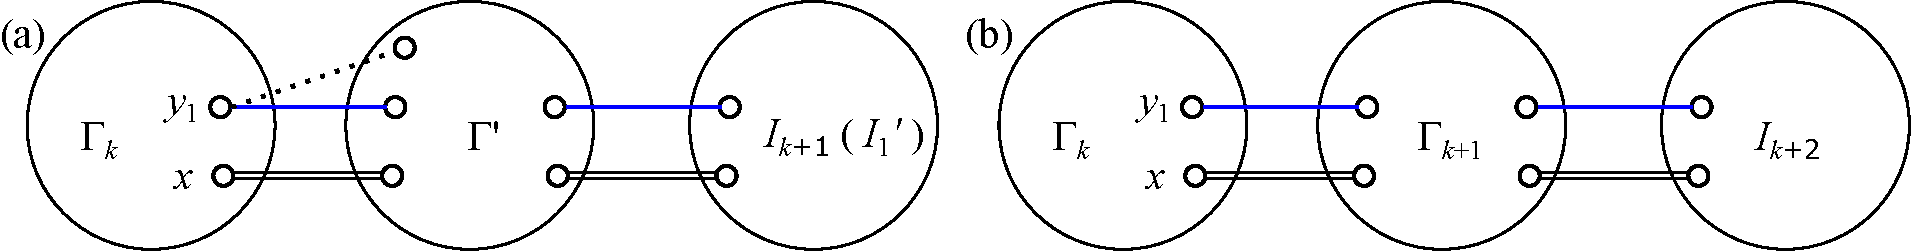
\includegraphics[width=15cm]{Recolli1.pdf}}
\ee
The graph (a) gives the isolated molecular subgraph $\Iso_k$ in $\wt{\cal G}$ with all red solid edges removed, where we have not merged the molecules connected by the dotted edge.  Inside the back circles are some subgraphs, where $\Gamma_k$ contains the molecules in $\Iso_k$ of the original graph $\cal G$, $\Iso'_1=\Iso_{k+1}$ is the first proper isolated subgraph in $(\cal G_{R})_{x,y_1 y_2}$ and also the $(k+1)$-th proper isolated subgraph in $\wt{\cal G}$, and $\Gamma'$ contains the molecules in $(\cal G_{R})_{x,y_1 y_2}$ that are not in $\Iso'_1$. 
%\iffalse
%Here the external dotted edge connects to $\Gamma'$ due to the following reason. Suppose we have an external dotted edge connected to a proper isolated subgraph, say $\Iso_i'$, in $(\cal G_{R})_{x,y_1 y_2}$. Then this dotted edge appears only when $\Iso'_i$ is connected with an external molecule through a $G$ edge during the expansions and we have added a dotted edge between them when applying $\cal O_{dot}$. 
%In this case, $\Iso_i'$ is not isolated anymore, which gives a contradiction. 
%\fi
The graph (b) is obtained from graph (a) by replacing the dotted edge with a blue solid edge and renaming the subgraphs; by Definition \ref{def moleg}, this does not change the molecular graph of $(\cal G_{R})_{x,y_1 y_2}$. (If the dotted edge is connected with $y_2$, then by Definition \ref{def moleg} it is counted as a red solid edge, so it is removed in graph (b).)


First, by the formula for the scaling order above, $\ord(\wt{\cal G})\ge \ord(\cal G) +1 $ follows from the fact that $(\cal G_{R})_{x,y_1 y_2}$ has scaling order $\ge 3$, and $\ge 5$ if $\epsilon=1$ and $(\cal G_{R})_{x,y_1 y_2}$ is a graph in $\PT^{(n-1)}$ (Definition \ref{def genuni2}). The only exception is the term with $\mathbf 1_{\al = y_1}\mathbf 1_{\al = y_2}$ when $y_1=y_2$: it replaces $t_{x,y_1y_1}$ with a constant multiple of $s_{xy_1}G_{y_1y_1}\overline G_{y_1y_1}$, which has the same scaling order as $t_{x,y_1y_1}$ and two fewer off-diagonal $G$ edges.
%we notice that the maximal subgraph of $(\cal G_P)_{x,y_1y_2}$ is not an isolated subgraph because it is connected with $x$ through a $\dashed$ edge, with $y_1$ through a blue solid edge, and with $y_1$ or $y_2$ through a dotted edge in the molecular graph.
%with its complement through a blue edge, a black $\dashed$ edge and a dotted edge. 
Second, using the fact that both $\cal G$ and $(\cal G_R)_{x,y_1y_2}$ have no proper strongly isolated subgraphs, we immediately get that \smash{$\wt{\cal G}$} also does not contain any proper strongly isolated subgraph. 
%Furthermore, with property (i) of Definition \ref{def genuni2}, it is easy to see that the atoms that are not standard neutral in the new graph all belong to the minimal isolated subgraph.
%except for the maximal isolated subgraph of $\cal G_1$. 
It remains to prove the SPD property of $\wt{\cal G}$. In $\wt{\cal G}$, the dotted edge merges a molecule containing $y_1$ (or $y_2$) with a molecule in $\Gamma'$, and these two molecules belong to different components of graph (b) (for $y_1$, to the two adjacent components $\Gamma_k$ and $\Gamma_{k+1}$). Hence with Lemma \ref{hard lemmdot}, it suffices to show that graph (b) in \eqref{eq_recolli1}, denoted by $\wt{\cal G}_b$, is SPD. In this graph, we have renamed $\Iso_{k+1}$ in (a) as $\Iso_{k+2}$ and $\Gamma'$ as $\Gamma_{k+1}$. Notice that $\Gamma_{k+1}$, $\Iso_{k+2}$ and the two edges between them form the isolated subgraph $\Iso_{k+1}$ in \smash{$\wt{\cal G}_b$}.
%In $\cal G_{new}$, the isolated subgraph $\Iso_k$ takes the form of the first graph in the following figure:  
%\be\label{eq_recolli1}
%\parbox[c]{0.9\linewidth}{\includegraphics[width=14cm]{Recolli1.png}}
%\ee
%Here we have not merged the molecules connected by the dotted edge $(x,\gamma)$. The subgraph inside the purple box is the maximal subgraph of $(\cal G_{R})_{x,y_1y_2}$, which is not isolated in $\cal G_{new}$ as discussed above. But it may contain proper isolated subgraphs, which will becomes the isolated subgraphs $I_{k+1} \supset I_{k+2} \supset \cdots$ in $\cal G_{new}$. 
%Moreover, the component $\Gamma_s$ is the subgraph induced on the molecules that are not in the maximal isolated subset of molecules in $(\cal G_{R})_{x,y_1y_2}$. Without loss of generality, we draw a dotted edge connecting $y_1$ to an atom in $\Gamma_s$---same proof also works if the dotted edge is connected to $y_2$. 
%Suppose we remove the dotted edge $(x,\gamma)$ in $\cal G_{new}$ and get a graph $\cal G_{new}'$. In the second graph of \eqref{eq_recolli1}, we draw the isolated subgraph $\Iso_k$ of $\cal G_{new}'$. 
%Now the molecules  in $\Gamma_s$ and $\Iso_{k+1}$ form an isolated subset of molecules in $\cal G_{new}'$, and we denote the subgraph induced on it as $\Iso'_{k}$. If we can show that $\cal G_{new}'$ is SPD, then using Lemma \ref{hard lemmdot} and the same argument as in the proof of Lemma \ref{lem localgood2}, we get that $\cal G_{new}$ is also SPD and hence conclude Lemma \ref{lem recolli}. 

%From the SPD properties of $\cal G$ and $(\cal G_{R})_{x,y_1y_2}$, we immediately obtain that $\cal G'_{new}$ satisfies property (iii) of Definition \ref{def seqPDG}. 

%For the SPD property of $\cal G_{new}'$, 
Now we verify the properties (i)--(iii) of Definition \ref{def seqPDG} for $\wt{\cal G}_b$. The property (i) follows from Lemma \ref{trivial_claim3}. 
%the facts that $b_1$ is redundant in the original graph $\cal G$, and that $(\cal G_{R})_{x,y_1y_2}$ satisfies properties (vi) and (vii) of Definition \ref{def genuni}.  
Using the SPD property of $(\cal G_{R})_{x,y_1y_2}$ given by Definition \ref{def genuni2}, we get that there is at most one sequence of isolated graphs in $\Iso_k$. Together with the SPD property of $\cal G$ and the fact that $\Iso_k$ is the MIS of $\cal G$, it concludes the property (ii) for $\wt{\cal G}_b$. 
%So $\cal G_{new}'$ also contains at most one chain of isolated graphs and satisfies . 
It remains to prove the property (iii). Suppose the sequence of proper isolated subgraphs in $\wt{\cal G}_b$ is 
\be\label{pf_chain_iso}\Iso_{l}\subset \cdots \subset \Iso_{k+2}\subset \Iso_{k+1} \subset  \Iso_k \subset \cdots \subset \Iso_1,\quad \text{for some} \ \ l\ge k,\ee
and for simplicity of notation, we denote the maximal subgraph by $\Iso_0$.   
%where $\Iso_{j+1}$ is a maximal isolated subgraph of $\Iso_{j}$ for any $j$. 
For $j\ge k+1$, if we replace $\Iso_{j+1}$ and its two external edges with a $\dashed$ edge, then $\Iso_j$ becomes pre-deterministic because $(\cal G_{R})_{x,y_1y_2}$ is SPD. %Similarly, if we replace $\Iso_{k+1}$ and its two external edges with a $\dashed$ edge, then $\Iso_k'$ becomes pre-deterministic. 
For $j\le k-1$, if we replace $\Iso_{j+1}$ and its two external edges with a $\dashed$ edge, then $\Iso_j$ becomes pre-deterministic because $\cal G$ is SPD. Finally, if we replace $\Iso_{k+1}$ and its two external edges with a $\dashed$ edge, then it corresponds to changing the first blue solid edge in a pre-deterministic order of $\Iso_k$ into a $\dashed$ edge. Hence $\Iso_k$ becomes pre-deterministic by Definition \ref{def PDG}. In sum, we get that $\wt{\cal G}_b$ is SPD, which concludes statement (2) of Lemma \ref{lem globalgood}. 

\vspace{5pt}
\noindent {\bf Proof of (4):} Using a similar argument as the one for $\wt{\cal G}_b$, we get that $\wt {\cal G}$ is SPD; here we use that the $\dashed$ edge at $\otimes$ in $(\cal G_{Q})_{x,y_1y_2}$ ends at an internal atom or at an external atom connected with an internal atom through a dotted edge, which follows from condition (E) if $(\cal G_{Q})_{x,y_1y_2}$ has an internal atom (Definition \ref{def genuni2}). Then the SPD property of the graphs on the right-hand side of \eqref{mlevelTgdef3_Q} follow from Lemma \ref{lem localgoodQ}. Since $x$, $y_1$ and $y_2$ are internal atoms of $\cal G$, the atom in the $Q$-label of $\wt{\cal G}$ is an internal atom; if $(\cal G_{Q})_{x,y_1y_2}$ has no internal atoms, then its $Q$-label is at $\oplus$ by Definition \ref{def genuni2}, so this atom is $y_1\in \Iso_k$. The fact that the atom in the $Q$-label of a $Q$-graph belongs to the MIS follows from Lemma \ref{Q_lemma}.

For the scaling orders, by the formula above and property (i) of Lemma \ref{Q_lemma}, all graphs on the right-hand side of \eqref{mlevelTgdef3_Q} have scaling orders $\ge \ord(\wt{\cal G})\ge \ord(\cal G)-2+\ord((\cal G_{Q})_{x,y_1y_2})-2\epsilon\ge \ord(\cal G)$, because $\ord((\cal G_{Q})_{x,y_1y_2})\ge 2$, and $\ord((\cal G_{Q})_{x,y_1y_2})\ge 4$ if $\epsilon=1$ (Definition \ref{def genuni2}). If the atom in the $Q$-label of $(\cal G_{Q})_{x,y_1y_2}$ is not $\oplus$ or $\ominus$ (or connected with them through dotted edges), then $\Gamma_0$ in \eqref{QG} contains no weights or edges attached to it, and property (iv) of Lemma \ref{Q_lemma} gives $\ord(\cal G_\omega)\ge \ord(\wt{\cal G})+1\ge \ord(\cal G)+1$. Otherwise, this atom becomes $y_1$ or $y_2$ after the replacement. If $y_1\ne y_2$, we use instead that such $Q$-graphs have scaling order $\ge 3$, so that $\ord(\wt{\cal G})\ge \ord(\cal G)+1$. If $y_1=y_2$, then $y_1$ is an atom of the locally standard MIS $\Iso_k$, which has no weights, and $y_1$ is a standard neutral atom of $\cal G$ whose two solid edges $G_{\al y_1}$ and $\overline G_{\al y_1}$ belong to $t_{x,y_1y_1}$; moreover, $\cal G$ has no dotted edges (see the proof of Lemma \ref{lemm expansionstrat}). So $\Gamma_0$ again contains no weights or solid edges attached to $y_1$, and property (iv) of Lemma \ref{Q_lemma} applies.

It remains to prove the weakly isolated property of (possible) proper isolated subgraphs in $\cal G_{\omega}$.




%\iffalse Note that $Q$-expansions are also local expansions in the sense that they %following sense. In the $Q$-expansions, 
%will not create new molecules. Furthermore, the $\dashed$ edges, waved edges, and dotted edges are not affected either. On the other hand, any solid $G$ edge between two different molecules, say $\cal M_1$ and $\cal M_2$, is either not affected or becomes a connected path of two $G$ edges between $\cal M_1$ and $\cal M_2$. Finally, new dotted edges or solid $G$ edges may be added to the graphs due to the expansions. In particular, the path connectivities of both the blue net and the black net are not affected, and in fact become ``better" due to the possible new edges. %{\cob (We need to discuss about these observations together with a precise definition of the $Q$-expansions.)} 
%Hence as Lemma \ref{local lemma}, this lemma also follows from Lemma \ref{lem localgood2} if $\cal G_s$ does not contain any real-isolated subgraph. 
%\fi 


We will use the following observation. Similar to local expansions, the $Q$-expansions do not create new molecules (by property (ii) of Lemma \ref{Q_lemma}), and every solid edge between two different molecules is either unchanged or becomes a path of two solid edges of the same charge between these two molecules; besides, new dotted or solid edges may be added. Hence every molecule of $\cal G_\omega$ is a union of molecules of $\wt{\cal G}$. Given a proper isolated subset of molecules $\Pol$ in $\cal G_\omega$, let $\wt\Pol$ be the set of molecules of $\wt{\cal G}$ that are contained in molecules of $\Pol$. Then every edge between $\wt\Pol$ and its complement in the molecular graph of $\wt{\cal G}$ gives an edge of the same type (blue solid, red solid or $\dashed$) between $\Pol$ and its complement in the molecular graph of $\cal G_\omega$, and different edges give different edges. Since $\wt{\cal G}$ is doubly connected and $\wt\Pol$ is a nonempty proper subset of internal molecules, $\wt\Pol$ is a proper isolated subset of molecules in $\wt{\cal G}$, and $\Pol$ has at least as many external red solid edges as $\wt\Pol$. 

If $(\cal G_{Q})_{x,y_1y_2}$ contains no strongly isolated subgraphs, then the argument for (2) shows that $\wt{\cal G}$ has no proper strongly isolated subgraphs, and by the above observation neither has $\cal G_\omega$. Hence we assume that $(\cal G_{Q})_{x,y_1y_2}$ contains strongly isolated subgraphs. Then we have the following molecular graph without red solid edges: 
\begin{equation}\nonumber
	\parbox[c]{0.8\linewidth}{\center
		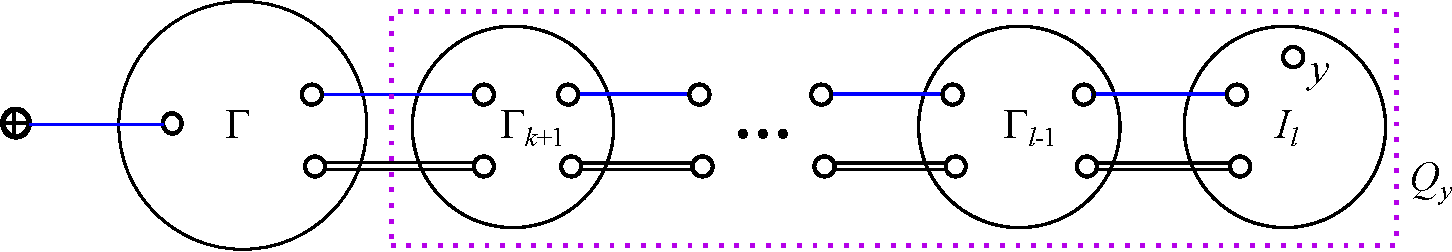
\includegraphics[width=12cm]{globalQ1.pdf}}
\end{equation}
Here all solid edges and weights inside the purple dashed rectangle have the same $Q_y$ label for the atom $y$ in the $Q$-label of $\wt{\cal G}$. Inside the back circles are some subgraphs, where $\Gamma$ contains the molecules in the original graph $\cal G$, and $\Gamma_i$'s are components corresponding to the isolated subgraphs in $(\cal G_{Q})_{x,y_1y_2}$. 
Again we denote the isolated subgraphs of $\wt{\cal G}$ by \eqref{pf_chain_iso}, where $\Iso_l$ with $l\ge k$ is the MIS. The isolated subgraphs $\Iso_i$, $1\le i\le k$, contain molecules of $\cal G$; counting the external edges as in the proof of (2), each of them has at least two external red solid edges, because $\cal G$ is globally standard. The isolated subgraphs $\Iso_i$, $k+1\le i\le l$, are induced on molecules of $(\cal G_{Q})_{x,y_1y_2}$, and they all contain the molecule of $y$, because $y$ belongs to the MIS of $(\cal G_{Q})_{x,y_1y_2}$ by Definition \ref{def genuni2}. (If the atom in the $Q$-label of $(\cal G_{Q})_{x,y_1y_2}$ is $\oplus$ or $\ominus$, or is connected with them through dotted edges, then $y$ is $y_1$ or $y_2$, the molecule of $y$ is a molecule of $\cal G$, and there is no such subgraph, i.e., $l=k$; in this case property (iv) of Lemma \ref{Q_lemma} is not needed below.)

Now let $\Pol$ be a proper isolated subset of molecules in $\cal G_\omega$, and let $\wt\Pol=\Pol(\Iso_i)$ be the corresponding proper isolated subset of molecules in $\wt{\cal G}$. If $i\le k$, then $\wt\Pol$, and hence $\Pol$, has at least two external red solid edges, i.e., $\Pol$ is weakly isolated. Suppose $k+1\le i\le l$. Then $y$ is an atom of $(\cal G_{Q})_{x,y_1y_2}$ that is not connected with $x$, $y_1$ or $y_2$ through dotted edges, so $\Gamma_0$ in \eqref{QG} does not contain any weights or edges attached to $y$. By property (iv) of Lemma \ref{Q_lemma} (in the precise form stated there), in $\cal G_{\omega}$ a weight or solid edge of $\Gamma_0$, whose atoms are atoms of $\cal G$ or external atoms and hence lie in molecules outside $\Pol$, (a) is split at $y$ into two red solid edges, (b) is split at $y$ into two blue solid edges, or (c) has an atom that has been identified with $y$. In case (c), this atom is not an internal atom of $\cal G$, because otherwise $\wt\Pol$ would contain a molecule of $\cal G$, and it is not $\otimes$, which carries no weights or solid edges. If $y$ is identified with $\oplus$, then by Definition \ref{def moleg} the dotted edge between them is counted as a blue solid edge, and the solid edge of $\Gamma_0$ at $\oplus$ is regarded as an edge at $y$, so this belongs to case (b). If $y$ is merged with $\ominus$, then by Definition \ref{def moleg} the dotted edge between them is counted as a red solid edge, so this belongs to case (a) instead of case (c). In case (b), $\Pol$ is connected with its complement through the two blue solid edges and an edge in the black net, which contradicts the assumption that $\Pol$ is isolated; in other words, the subgraphs $\Iso_{i}$, $k+1\le i \le l$, are not isolated anymore. In case (a), we have the following graph (or some variants of it, where we are not trying to draw all possible cases):
\begin{equation}\nonumber
	\parbox[c]{0.8\linewidth}{\center
		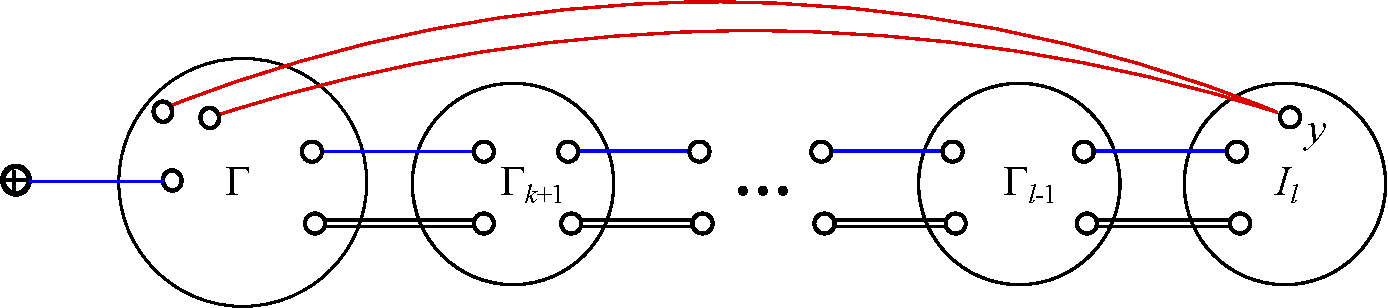
\includegraphics[width=11cm]{globalQ2.pdf}}
\end{equation}
In this case, $\Pol$ has at least two external red solid edges, so any subgraph $\Iso_{i}$, $k+1\le i \le l$, is weakly isolated if it is still an isolated subgraph in $\cal G_\omega$. In sum, we see that $\cal G_{\omega}$ does not contain proper strongly isolated subgraphs, and hence is globally standard. 
\end{proof}


   
%For this purpose, we introduce the concept of globally standard graphs. In each globally standard graph, there is a canonical order of all the $T$-variables. Then roughly speaking, the core reason why our global expansion strategy works is that every globally standard graph can be expanded, while each expansion of a globally standard graph still gives globally standard graphs as long as we expand the {\bf first} $T$-variable in it.  
%{\color{red} explain the ideas of solving equations for $T$}


\subsection{Global expansion strategy} \label{sec expandlvl40}



%The above lemma shows that the local expansions preserve the local standard property of graphs. Later we will show that the global standard property will be preserved as long as we expand the {\bf first} blue solid edge in the pre-deterministic order of the minimal isolated subgraph at each step. Then roughly speaking, the core argument of our proof is to show that every globally standard graph can be expanded, while each expansion of a globally standard graph still gives globally standard graphs. % as long as we expand the {\bf first} $T$-variable in it.

Lemma \ref{lem globalgood} gives a canonical choice of the standard neutral atom in a global expansion of a globally standard graph, that is, we choose an ending atom of the first blue solid edge in a pre-deterministic order of the MIS. With this choice, we define the global expansion strategy for the proof of Theorem \ref{incomplete Texp} in this subsection. 

%Now we describe the global expansion strategy to obtain the incomplete $T$-expansions up to any order. Roughly speaking, we use a repeated substitution procedure. Recall that after the local expansions, all the graphs are locally standard, such that each of them consists of generalized $T$-variables only. Also recall that we have defined the $k$-th order $T$-expansion for $2\le k \le n-1$. Then given any locally standard graph, we pick one generalized $T$-variable, and replace it with the $(n-1)$-th order $T$-expansion. We repeat this substitution until all the graphs can be written as the right-hand side of \eqref{mlevelTgdef incomp}. The most delicate part of this process is the choice of the generalized $T$-variable, and now we can give a concise description of this choice using the concepts define above: we choose the $T$-variable containing the {\bf first} solid blue edge in the {\bf pre-deterministic order} of the {\bf minimal isolated subgraph}.
 
%We have defined the second and third order $T$-expansions in Section \ref{sec Thetaexp}. Then we define the higher order $T$-expansion iteratively. Suppose for a fixed $n\in \N$, we have define the $k$-th order $T$-expansions for all $2\le k \le n-1$. 
%Applying the previous basic local expansions in Section \ref{sec_basiclocal} repeatedly will expand all the graphs into locally standard graphs. We expand the graphs as in the following chart in Figure \ref{Fig chart1}. %The outputs will be graphs satisfying the stopping rule or level 1 standard graphs. 
%Given a cut-off order $n$, suppose we have define the $k$-th order $T$-expansions for all $2\le k \le n-1$. 

Fix any $n\in \N$. As an induction hypothesis, suppose we have obtained the $(n-1)$-th order $T$-expansion. 
%Given $n\in \N$ in Theorem \ref{incomplete Texp}, 
Then we define the following stopping rules. We stop the expansion of a graph if it is a normal regular graph and satisfies at least one of the following properties:
\begin{itemize}
\item[(S1)] it is a $\oplus$/$\ominus$-recollision graph; %\hty{ we stop whenever a resollision? we dont care order? } 

\item[(S2)] its scaling order is at least $n+1$;

\item[(S3)] it is a $Q$-graph; % (recall Definition \ref{Def_recoll}); %\hty{ I thought that $Q$ graphs still need to expand? } 

\item[(S4)] it is \emph{non-expandable}, that is, it is locally standard and has no redundant blue solid edge. % plus \hty{do we need plus? or we want to use blue? } $G$ edge in the maximal subgraph. \hty{ why max subgraph instead of just saying no redundant edge? } 
\end{itemize}
If a graph has a deterministic maximal subgraph, then it is non-expandable. On the other hand, in a non-expandable graph that is not deterministic, we cannot expand a plus $G$ edge without breaking the doubly connected property. Moreover, no expansion (including $\cal O_{dot}$) is applied to a graph of scaling order $>D$: such a graph is sent to the outputs directly. We also remark that, except for the $Q$-graph $- m Q_{\fb_1} ( \Theta_{\fa\fb_1} \overline G_{\fb_1 \fb_2})$ in \eqref{QT>2}, which satisfies (S3), all graphs in the expansions below have the charge pattern defined before Definition \ref{def genuni2} (see the proof of Lemma \ref{lemm expansionstrat}). Now we give our global expansion strategy. %The core of the expansion strategy is to expand the plus $G$ edges according to the pre-deterministic order in the minimal isolated subgraph, such that the graphs appearing in the expansions are globally standard if they do not satisfy the stopping rules (S1)-(S3) already. 
%Here by ``good", we mean the graph is sequentially pre-deterministic, and does not contains any non-deterministic real-isolated subgraph except for the maximal isolated subgraph $I_0$.

%For simplicity of presentation, we introduce the following notion. 
%\begin{definition}[``Good" graphs]\label{defn goodgraph}
%We say a graph is ``good" if it has no $Q$-labels and satisfies the following properties:
%\begin{itemize}
%\item[(1)] it is doubly connected;
%\item[(2)] it contains at most one chain of non-deterministic isolated graphs, and is sequentially pre-deterministic;
%\item[(3)] it contains no real-isolated subgraph (that is, the chain of isolated graphs can only be pseudo-isolated).
%\end{itemize}  
%\end{definition}

%Then the expansion strategy is as follows.

\begin{strategy}[Global expansion strategy]\label{strat_global}
Fix any $n\in \N$ and large $D>n$. Given the above stopping rules (S1)--(S4), we apply the following strategy.
%\noindent{\bf Global expansion strategy for $n$-th order $T$-expansion:}
 \vspace{5pt}

\noindent{\bf Step 0}: We start with the second order $T$-expansion \eqref{seconduniversal}, and apply local expansions to obtain a linear combination of new graphs, each of which either satisfies the stopping rules (S1)--(S3) already, or is locally standard. At this step, there is only one internal molecule in every graph, which is trivially globally standard. %by Lemma \ref{lem localgood2}. (actually all the plus $G$ edges are short edges within one single molecule).   

\vspace{5pt}
\noindent{\bf Step 1}: Given a globally standard input graph, we perform the local expansions in Definitions \ref{Ow-def}, \ref{multi-def}, \ref{GG-def} and \ref{GGbar-def} on atoms in the minimal isolated subgraph (MIS). We apply $\cal O_{GG}^{(x)}$ in the form whose waved edge in the main term connects $x$ with an internal atom (if the atom $y$ in Definition \ref{GG-def} is an external atom, this is the form of \eqref{Oe2x} with all $G$ entries transposed). We send the resulting graphs that already satisfy the stopping rules (S1)--(S4) to the outputs. Every remaining graph is globally standard by Lemma \ref{lem localgood3}, and its MIS %\hty{ it might be better to spell out mim isolated}  
is locally standard (i.e. the MIS has no weights and every atom in it either has degree 0 or is a standard neutral atom by Definition \ref{deflvl1}).

\vspace{5pt}
\noindent{\bf Step 2}: Given a globally standard input graph $\cal G$ with a locally standard MIS, say $\Iso_k$, we find a $t_{x,y_1y_2}$ or $t_{y_1y_2,x}$ variable defined in \eqref{12in4T}, so that $\al$ is a standard neutral atom in $\Iso_k$ and the blue solid edge $G_{\al y_1}$ or $G_{y_1 \al}$ is the first blue solid edge in a pre-deterministic order of $\Iso_k$. %\hty{ Maybe we just use $\cal I$ for $\Iso$}
More precisely, if $G_{pq}$ is the first blue solid edge in a pre-deterministic order of $\Iso_k$, then we take $\al=q$ and the variable $t_{y_1y_2,x}$, where $y_1=p$, $\overline G_{y_2 q}$ is the red solid edge at $q$, and $s_{qx}$ is the waved edge at $q$. By the charge pattern of $\cal G$, $x$, $y_1$ and $y_2$ are internal atoms. (The input graph $\cal G$ is not a $\oplus$/$\ominus$-recollision graph, has only $\dashed$ edges at $\otimes$, and has scaling order $\ge 4$; see the proof of Lemma \ref{lemm expansionstrat}.)
If we cannot find such a $t$-variable, then we stop expanding the input graph.

\vspace{5pt}
\noindent{\bf Step 3}: We apply the global expansions defined in Section \ref{subsec global} to the $t_{x,y_1y_2}$ or $t_{y_1y_2,x}$ variable chosen in Step 2. More precisely, we first replace $t_{x,y_1y_2}$ (or $t_{y_1y_2,x}$) with \eqref{replaceT} (or an expression obtained by taking transpositions of all $G$ entries in \eqref{replaceT}; the waved, $\dashed$ and labelled $\dashed$ edges are not transposed), and write the resulting graphs as normal regular graphs using $\cal O_{dot}$. Then we apply the $Q$-expansions defined in Section \ref{sec defnQ} to graphs that take the form \eqref{QG}, where both $\Gamma_0$ and \smash{$\wt\Gamma_0$} are non-trivial. 
%\hty{ non-$Q$ graph (i.e., $\Gamma_0$) in the expression} 
%\hty{this all depends on how you define $Q$ expansion? in my mind, it is applied to the graph $\cal G_0$. but you seem to have a different thing in mind}
We send the resulting graphs that already satisfy the stopping rules (S1)--(S4) to the outputs. The remaining graphs are all globally standard by Lemma \ref{lem globalgood}, and we sent them back to Step 1. 
\end{strategy}

Using the definition of globally standard graphs, it is easy to show that if an output graph from the above strategy does not satisfy the stopping rules (S1)--(S3), then it must have a deterministic maximal subgraph. 
\begin{lemma}\label{lemm expansionstrat_nonstop}
Let $\cal G_{\fa,\fb_1\fb_2}$ be an output graph from the global expansion strategy \ref{strat_global}. If $\cal G_{\fa,\fb_1\fb_2}$ does not satisfy stopping rules (S1)-(S3), then it has a deterministic maximal subgraph with a doubly connected structure. %except for the two edges connected with $\oplus$ and $\ominus$.
\end{lemma}
\begin{proof}
By Lemma \ref{lem localgood3} and Lemma \ref{lem globalgood}, we know that $\cal G_{\fa,\fb_1\fb_2}$ is globally standard. Under the assumption of this lemma, $\cal G_{\fa,\fb_1\fb_2}$ either is non-expandable or does not contain a $t$-variable required by Step 2 of Strategy \ref{strat_global}. In either case, $\cal G_{\fa,\fb_1\fb_2}$ contains a locally standard MIS, say $\Iso_k$, which, by the pre-deterministic property of $\Iso_k$, does not contain any internal blue solid edge. 

Now we consider two cases. First, suppose $\Iso_k$ is a proper isolated subgraph. Due to the weakly isolated property, $\Iso_k$ is connected with at least two external red solid edges and at most one blue solid edge. Hence $\Iso_k$ contains a non-standard neutral atom, which gives a contradiction. Second, suppose $\Iso_k$ is indeed the maximal subgraph of $\cal G_{\fa,\fb_1\fb_2}$. Then $\Iso_k$ is locally standard and does  not contain any internal blue solid edges, so it is deterministic.
%\iffalse
%Then we prove the second statement, that is, for a non-expandable graph $\cal G$ that does not satisfy other stopping rules, it must be deterministic except for the two edges connected with $\oplus$ and $\ominus$.
%	By Lemmas \ref{local lemma}-\ref{hard lemma}, we know that $\cal G$ is sequentially pre-deterministic and does not contain any real-isolated subgraph except for the maximal isolated subgraph $I_0$. Let $I_k$ be the minimal non-deterministic isolated subgraph of $\cal G$. To prove the second statement, we first claim that $I_k$ is the maximal isolated subgraph $I_0$. %and does not satisfy other stopping rules and  only if $\cal G$ 
%	Suppose $I_k\subsetneq I_0$. 
%	%Then $\cal G$ contains at least one plus $G$ edge---otherwise $I_k$ must be deterministic since $\cal G$ is locally standard. 
%	By the sequentially pre-deterministic property of $I_k$, in order for $\cal G$ to be non-expandable, we must have that $I_k$ does not contain any plus $G$ edge. 
%	% a deterministic isolated subgraph, say $I_{k+1}$, that is connected to other molecules in $I_k$ through a plus $G$ edge and some minus $\overline G $ edges. But 
%	Then as shown in the proof of Lemma \ref{lem leading}, $I_{k+1}$ contains an atom that is connected with at least two minus $G$ edges since $I_{k+1}$ is pseudo-isolated. Hence $\cal G$ cannot be locally standard, which gives a contradiction. This concludes the claim $I_k=I_0$. Now by the sequentially pre-deterministic property of $I_0$, we see that $I_0$ does not contain any plus $G$ edge. Together with the fact that $\cal G$ is locally standard, it implies that $I_0$ is a deterministic subgraph. This concludes the second statement.
%	
%	{\cor Moreover, if $I_k$ contains no plus $G$ edge after the replacement and $I_k$ is not the maximal isolated subgraph $ I_0$, then it contains an atom that is connected with at least two minus $G$ edges. 
%		
%		For the second statement, we first consider the case $y_1\ne y_2$.  Since $\cal G$ is locally standard, the two end atoms of $b_1$ are connected with two minus $G$ edges. Thus after the replacement, the atom $y_1$ is connected with two minus $G$ edges. On the other hand, suppose $y_1=y_2$. If $I_k$ contains no plus $G$ edge after the replacement, then $b_1$ must be the last plus $G$ edge in $I_k$. However, recall that $I_k$ is pseudo-isolated so that it is connected with its complement through more than one minus $G$ edges and only one plus $G$ edge. Then there exists a non-neutral atom in $I_k$,  which contradicts the fact that $\cal G$ is locally standard. 
%	}
%\fi
\end{proof}

With Lemma \ref{lem globalgood}, we show that Strategy \ref{strat_global} will stop after $\OO(1)$ many iterations.

\begin{lemma}\label{lemm expansionstrat}
The expansions in Strategy \ref{strat_global} will stop after at most $C_n$ many iterations of Steps 1--3, where $C_n$ denotes a large constant depending on $n$. All graphs from these expansions are doubly connected. If a graph satisfies the stopping rule (S1)/(S2)/(S3) and has scaling order $\le D$, then it satisfies the property (i)/(ii)/(iii) of Definition \ref{def genuni2}. All output graphs satisfy the property (iv) of Definition \ref{def genuni2}.
\end{lemma}
\begin{proof}
We first note that the properties in Definition \ref{defn genuni} concerning the external atoms, condition (E) and the charge pattern are preserved in the expansions: the local expansions and $Q$-expansions act on internal atoms, and in Step 3 the replacement is at the internal atoms $x$, $y_1$, $y_2$ (see Step 2), so it does not change the edges at the external atoms (and the waved edges in the graphs of the $T$-expansion connect internal atoms by Definition \ref{def genuni2}). In particular, every graph in the expansions that has an internal atom, including the $Q$-graphs, satisfies the following property: if $\ominus$ is not connected with an internal atom through dotted edges, then there is a red solid edge $\overline G_{u\fb_2}$ (possibly with a $Q$-label), where $u$ is an internal atom or an atom connected with an internal atom through dotted edges. Indeed, this property holds for the graphs in \eqref{Aho>2} and \eqref{QT>2} that have internal atoms, and every step of the expansions keeps it: a local expansion keeps the edge $\overline G_{u\fb_2}$, or replaces it by edges $\overline G_{v\fb_2}$ with internal atoms $v$; $\cal O_{dot}$ keeps it, unless $u$ is identified with $\fb_2$, in which case $\ominus$ becomes connected with an internal atom through dotted edges; the replacement in Step 3 does not change the edges at the external atoms; and the $Q$-expansions do not decrease the number of red solid edges between the internal molecules and $\ominus$ (by the observation in the proof of Lemma \ref{lem globalgood} (4)), where these edges take the form $\overline G_{v\fb_2}$ by the charge pattern. Moreover, the local expansions, $\cal O_{dot}$ and the $Q$-expansions map internal atoms to internal atoms, and in Step 3 the atom $x$ of the input graph remains an internal atom, so an output graph without internal atoms is one of the input graphs in \eqref{QT>2} without internal atoms, i.e. one of the two normal regular graphs obtained from $- m Q_{\fb_1} ( \Theta_{\fa\fb_1} \overline G_{\fb_1 \fb_2})$ using $\cal O_{dot}$, which satisfy the stopping rule (S3) and have the red solid edge $\overline G_{\fb_1\fb_2}$ or the dotted edge between $\fb_1$ and $\fb_2$ at $\ominus$. This gives the part of property (ix) of Definition \ref{defn genuni} at $\ominus$ for all output graphs, including the $Q$-graphs. Moreover, the dotted edges in every graph form a forest, as required in Definition \ref{defn genuni}, since the graphs are written as normal regular graphs using $\cal O_{dot}$ (after merging, the dotted edges in each block of atoms connected by dotted edges form a tree). Next, the scaling order does not decrease in the expansions (by \cite[Lemmas 3.9, 3.13, 3.16 and 3.19]{PartI_high} for the local expansions, property (i) of Lemma \ref{Q_lemma} for the $Q$-expansions, and Lemma \ref{lem globalgood} for the replacements in Step 3), and the graphs in \eqref{Aho>2} and \eqref{QT>2} have scaling orders $\ge 3$ and $\ge 2$, respectively, so every graph in the expansions that is not a $Q$-graph has scaling order $\ge 3$. Suppose $\oplus$ and $\ominus$ are connected by a path of dotted edges in an output graph. If this graph is one of the input graphs in \eqref{Aho>2} and \eqref{QT>2} written as normal regular graphs, then one checks directly that its scaling order is $\ge 5$ if it is not a $Q$-graph, and $\ge 4$ if it is a $Q$-graph (the dotted edges at $\oplus$ and $\ominus$ replace off-diagonal solid edges; for $- m Q_{\fb_1} ( \Theta_{\fa\fb_1} \overline G_{\fb_1 \fb_2})$, the dotted edge between $\fb_1$ and $\fb_2$ replaces $\overline G_{\fb_1 \fb_2}$). Otherwise, the path has been created by an expansion of a graph in which $\oplus$ and $\ominus$ are not connected by dotted edges. The replacement in Step 3 does not create such a path, because it is applied at the internal atoms $x$, $y_1$, $y_2$ of a graph that has no dotted edges (see below). In a local expansion in Step 1, the path is created by $\cal O_{dot}$, and each of the two dotted edges at $\oplus$ and $\ominus$ replaces an off-diagonal solid edge, which increases the scaling order by $1$ compared with the graph with a $\times$-dotted edge instead; hence the new graph has scaling order $\ge 3+2=5$. In a $Q$-expansion in Step 3, a new dotted edge at $\oplus$ or $\ominus$ either replaces an off-diagonal solid edge in $\cal O_{dot}$, or is added in the splitting $1=\mathbf 1_{u=x}+\mathbf 1_{u\ne x}$ of Section \ref{sec defnQ} with $u\in\{\fb_1,\fb_2\}$; in both cases the scaling order increases by at least $1$, so the new graph has scaling order $\ge \ord(\wt{\cal G})+1\ge 5$, where $\wt{\cal G}$ is the graph obtained from the replacement in Step 3, which has scaling order $\ge 4$ by the proof of Lemma \ref{lem globalgood} (4). In sum, such an output graph has scaling order $\ge 5$ if it is not a $Q$-graph, and $\ge 4$ if it is a $Q$-graph. This gives the property (iv) of Definition \ref{def genuni2}. We have also shown that an expansion step that produces a graph in which $\oplus$ and $\ominus$ are connected by dotted edges from a graph in which they are not strictly increases the scaling order; this will be used in Section \ref{sec expandlvl4}.

Let $\cal G$ be an input graph for Step 3 of Strategy \ref{strat_global}. %From the second order $T$-expansion \eqref{seconduniversal}, we see that $\ord(\cal G)$
By Lemmas \ref{lem localgood3} and \ref{lem globalgood} and the above discussion, $\cal G$ is globally standard, satisfies condition (E), has the charge pattern and has only $\dashed$ edges at $\otimes$; it is not a $\oplus$/$\ominus$-recollision graph by (S1), its MIS is locally standard by Step 1, and $y_2$ is an internal atom by Step 2. Moreover, $\ord(\cal G)\ge 4$. First, $\cal G$ has no dotted edges: by Definition \ref{defnlvl0} (iii), a dotted edge has an external atom; it is not at $\otimes$, which only has a $\dashed$ edge; it does not connect $\oplus$ or $\ominus$ with an internal atom, since $\cal G$ is not a $\oplus$/$\ominus$-recollision graph; and it does not connect $\oplus$ with $\ominus$ by condition (E). Let $n_0$ be the number of internal atoms of $\cal G$. By Definition \ref{defnlvl0} (ii) and the $\dashed$ edge at $\otimes$, the internal atoms and $\otimes$ are connected through $a\ge n_0$ waved and $\dashed$ edges. The graph obtained by removing the two solid edges of the $t$-variable chosen in Step 2 is still connected (these edges connect internal atoms), and $\times$-dotted edges only connect atoms that are connected by solid edges; hence the $n_0+3$ atoms of $\cal G$ are connected through the waved, $\dashed$ and solid edges other than these two solid edges, whose number $a+b$ is at least $n_0+2$, where $b$ is the number of these solid edges. By \eqref{eq_deforderrandom2}, we obtain that $\ord(\cal G)\ge 2a+b+2-2n_0\ge a+(n_0+2)+2-2n_0\ge 4$. Hence $\cal G$ satisfies the assumptions of Lemma \ref{lem globalgood}. The new graphs from case (3) of Lemma \ref{lem globalgood} with $\epsilon=0$ are SPD and have scaling orders $\ge n + 1$, so it satisfies the property (ii) of Definition \ref{def genuni2}, while those with $\epsilon=1$ are globally standard; the new graphs from case (5) of Lemma \ref{lem globalgood} are doubly connected and have scaling orders $\ge D + 1$. In general, the graphs of scaling order $>D$ are written as normal regular graphs using $\cal O_{dot}$ when they are created (in Step 1 or Step 3), and are not expanded further; they are included into $\Err_{n,D}$, so the graphs in $\Err_{n,D}$ are normal regular. Furthermore, the new graphs from cases (1) and (2) of Lemma \ref{lem globalgood}, and from case (3) with $\epsilon=1$, are globally standard, so they satisfy the property (i)/(ii) of Definition \ref{def genuni2} if they satisfy the stopping rule (S1)/(S2). Finally, in equation \eqref{mlevelTgdef3_Q}, the graphs in $\cal Q$ satisfy the stopping rule (S3) and the property (iii) of Definition \ref{def genuni2}; the graphs in $\cal G_{err}$ are doubly connected and have scaling orders $\ge D+1$; the graphs $\cal G_{\omega}$ are globally standard, so they satisfy the property (i)/(ii) of Definition \ref{def genuni2} if they satisfy the stopping rule (S1)/(S2). Combining the above discussions with Lemma \ref{lem localgood3} for local expansions in Step 1 of Strategy \ref{strat_global}, we conclude the second and third statements. 
	
Now we prove the first statement. Let $\cal G_0$ be a graph from Step 0. We construct inductively a tree diagram $\cal T$ for the  expansions of $\cal G_0$ as follows. Let $\cal G_0$ be the root. Given a graph $\cal G$ represented by a vertex of the tree, its children are the graphs obtained from an iteration of Steps 1--3 of Strategy \ref{strat_global} acting on $\cal G$. Suppose a graph $\cal G$ satisfies a stopping rule, then we stop the expansion and $\cal G$ has no children on $\cal T$. Let the height of $\cal T$ be the maximum distance between the root and a leaf of $\cal T$. To show that the expansions will stop after $C_n$ many iterations of Steps 1--3, it is equivalent to show that $\cal T$ is a finite tree with height $\le C_n$.
	
Let $\cal G_0 \to \cal G_1 \to \cal G_2 \to \cdots \to \cal G_h$ be a self-avoiding path from the root to a leaf. Let $k_0=0$. After having defined $k_i$, let $k_{i+1}:=h\wedge \min\{j> k_i : \text{ord}(\cal G_j) > \text{ord}(\cal G_{k_i})\}$. Then the increasing sequence $\{k_0,k_1, k_2, \cdots\}$ has length at most $n$, because a graph of scaling order $\ge n+1$ satisfies the stopping rule (S2) and has no children. Moreover, we claim that $|k_{i+1}-k_i|\le C'_n$ for a constant $C'_n$ depending on $n$. Consider the expansions (the local expansions in Step 1, and the replacements and $Q$-expansions in Step 3) performed in the iterations from $\cal G_{k_i}$ to $\cal G_{k_{i+1}-1}$, which keep the scaling order $\ord(\cal G_{k_i})$ along the path. We claim that each of them strictly decreases the triple
$$\left(\#\{\text{light weights}\},\ \#\{\text{off-diagonal solid edges}\},\ \mu\right)$$
in the lexicographic order, where $\mu$ is the quantity used in the proof of \cite[Lemma 3.22]{PartI_high} to show that the local expansions terminate. Indeed, at a fixed scaling order, the local expansions do not create new light weights (new light weights only appear in graphs of strictly higher scaling orders), and the weight expansion of a light weight removes it (\cite[Lemma 3.9 (b)]{PartI_high}); the edge expansions in \cite[Lemmas 3.13, 3.16 and 3.19]{PartI_high} do not increase the number of solid edges, and when the first two coordinates are unchanged, $\mu$ decreases as in the proof of \cite[Lemma 3.22]{PartI_high}; finally, the graphs from Step 3 with the same scaling order as the input graph (the graphs obtained from $m\Theta_{xy_1}\overline G_{y_1y_2}$ in case (1) of Lemma \ref{lem globalgood}, and the exceptional graphs in case (2) of Lemma \ref{lem globalgood} when $y_1=y_2$) have the same light weights and fewer solid edges. Since every light weight and every off-diagonal solid edge contribute $1$ to the scaling order, and the number of internal atoms is at most the number of waved and $\dashed$ edges by the property (ii) of Definition \ref{defnlvl0}, the first two coordinates are at most $n$; then $\mu$ is bounded in terms of $n$ as in the proof of \cite[Lemma 3.22]{PartI_high}. This concludes the claim. In sum, we have shown that $h\le nC'_n$, i.e. the height of $\cal T$ is at most $nC'_n$.
\end{proof}





\subsection{Proof of Theorem \ref{incomplete Texp}}\label{sec expandlvl4}

In this subsection, we prove Theorem \ref{incomplete Texp} using the results in Sections \ref{sec_global_standard} and \ref{sec expandlvl40}. To summarize, we have proved the following facts.
\begin{itemize}
\item[(I)] The expansions of $T_{\fa,\fb_1\fb_2}$ will stop and give $\OO(1)$ many new graphs (Lemma \ref{lemm expansionstrat}). 

%\item[(II)] If a new graph from the expansions does not satisfy the stopping rules, then it is globally standard (Lemma \ref{lem localgood3} and Lemma \ref{lem globalgood}). 

\item[(II)] If a new graph from the expansions satisfies the stopping rule (S1)/(S2)/(S3), then it satisfies the property (i)/(ii)/(iii) of Definition \ref{def genuni2}; all new graphs satisfy the property (iv) of Definition \ref{def genuni2} (Lemma \ref{lemm expansionstrat}).

\item[(III)] If a new graph from the expansions does not satisfy the stopping rules (S1)--(S3), then it has a deterministic doubly connected maximal subgraph (Lemma \ref{lemm expansionstrat_nonstop}).
\end{itemize}

Now we complete the proof of Theorem \ref{incomplete Texp} using induction. We have obtained the second order $T$-expansion and $\incomp$ in \eqref{seconduniversal}. Fix any $ 2\le n\le M$. Suppose for all $2\le k \le n-1$, we have constructed the $k$-th order $\incomp$ using Strategy \ref{strat_global}, shown the properties \eqref{two_properties0}--\eqref{3rd_property0} of $\Sele_{k}$ (for $k\ge 4$) by Lemma \ref{cancellation property}, and obtained the $k$-th order $T$-expansion using Corollary \ref{lem completeTexp}. Now applying Strategy \ref{strat_global}, we obtain the following expansion of $T_{\fa,\fb_1\fb_2}$: %can be expanded into %the form %that is similar to \eqref{mlevelTgdef incomp}: %with $n$ replaced by $k$, 
\begin{align} 
 T_{\fa,\fb_1 \fb_2}&= m  \Theta_{\fa \fb_1} \overline G_{\fb_1\fb_2} + \sum_{x} (\Theta \wtSdelta^{(n)})_{\fa x} t_{x,\fb_1\fb_2} + (\wtPIT^{(n)})_{\fa,\fb_1 \fb_2} +  (\AIT^{(>n)})_{\fa,\fb_1\fb_2}  + (\QIT^{(n)})_{\fa,\fb_1\fb_2}+  (\Err'_{n,D})_{\fa,\fb_1\fb_2} .\nonumber
\end{align}
Here the second term collects the output graphs in (III). By Lemma \ref{lemm expansionstrat_nonstop}, the charge pattern and the property at $\ominus$ shown in the proof of Lemma \ref{lemm expansionstrat}, each of these graphs consists of a deterministic graph between $\otimes$ and an atom $x$ and the variable $t_{x,\fb_1\fb_2}$, which gives the above form (we discard the graphs containing a $\times$-dotted edge between an atom and itself, which vanish).
Denoting
$$
	(\PIT^{(n)})_{\fa,\fb_1 \fb_2}=	(\wtPIT^{(n)})_{\fa,\fb_1 \fb_2} -   \sum_{x } (\Theta  \wtSdelta^{(n)})_{\fa x} |m|^2 \sum_\al s_{x\al} G_{\al\fb_1}\overline G_{\al\fb_2}\left(1- \mathbf 1_{\al \ne \fb_1}\mathbf 1_{\al\ne \fb_2} \right),
$$
the above equation can be rewritten as 
\begin{align} 
T_{\fa,\fb_1 \fb_2}&= m  \Theta_{\fa \fb_1} \overline G_{\fb_1\fb_2} + \sum_{x } (\Theta \wtSdelta^{(n)})_{\fa x} T_{x,\fb_1\fb_2} +  (\PIT^{(n)})_{\fa,\fb_1 \fb_2} +  (\AIT^{(>n)})_{\fa,\fb_1\fb_2} \nonumber\\
&+ (\QIT^{(n)})_{\fa,\fb_1\fb_2}+  (\Err'_{n,D})_{\fa,\fb_1\fb_2}. \label{add_incompT}
\end{align}
%such that properties (i) and (vi) of Definition \ref{def incompgenuni} holds and
%\begin{enumerate}
%\item $(\wtPIT^{(k)})_{\fa,\fb_1\fb_2}$ is a sum of at most $C_k$ many $\oplus/\ominus$-recollision graphs, each of which is of scaling order $\le k$, is globally standard, and has no $P$ or $Q$ labels; 
%
%\item $(\AIT^{(>k)})_{\fa,\fb_1\fb_2}$ is a sum of at most $C_k$ many graphs, each of which is of scaling order $> k$, is SPD, and has no $P$ or $Q$ labels;  
%
%\item $(\QIT^{(k)})_{\fa,\fb_1\fb_2} $ is a sum of at most $C_k$ many $Q$-graphs, such that each of them is SPD, and  the atom in the $Q$-label in every graph belong to the minimal isolated subgraph of it;
%
%\item $\wtSdelta^{(k)}$ is a sum of at most $C_k$ many {\bf doubly connected} deterministic graphs of scaling order $ \le k$, where the labelled $\dashed$ $\Theta$ edges can only be of the form $\Theta \Sele_{2k_1}\Theta  \Sele_{2k_2}\Theta \cdots \Theta  \Sele_{2k_l}\Theta$ with $4\le 2k_i \le n-1$.
%\end{enumerate}
%Here in (iv), the doubly connected property of the graphs in $\wtSdelta^{(k)}$ follows from the fact that the graphs that will contribute to $\wtSdelta^{(k)}$ are all globally standard (and hence doubly connected). 
%%if they are not in $(\wtPIT^{(k)})_{\fa,\fb_1\fb_2}$, $(\AIT^{(>k)})_{\fa,\fb_1\fb_2}$ or $(\QIT^{(k)})_{\fa,\fb_1\fb_2}$. 
%%Using $\mathbf 1_{\al\ne \fb_1}\mathbf 1_{\al\ne \fb_2}=1-\mathbf 1_{\al=\fb_1} \mathbf 1_{\al\ne\fb_2} -  \mathbf 1_{\al\ne\fb_1} \mathbf 1_{\al = \fb_2}-\mathbf 1_{\al= \fb_1}\mathbf 1_{\al = \fb_2}$, 
%We can write the second term on the right-hand side of \eqref{add_incompT} as  
% \begin{align*}
% & \sum_{x } \left(\Theta \wtSdeltan\right)_{\fa x} |m|^2 \sum_\al s_{x\al} G_{\al\fb_1}\overline G_{\al\fb_2}\mathbf 1_{\al\ne \fb_1}\mathbf 1_{\al\ne \fb_2}  =  \sum_{x } \left(\Theta \wtSdeltan\right)_{\fa x} T_{x,\fb_1\fb_2}\\
% &-   \sum_{x } \left(\Theta \wtSdeltan\right)_{\fa x} |m|^2 \sum_\al s_{x\al} G_{\al\fb_1}\overline G_{\al\fb_2}\left(\mathbf 1_{\al = \fb_1}\mathbf 1_{\al\ne \fb_2} +\mathbf 1_{\al\ne \fb_1}\mathbf 1_{\al = \fb_2} +\mathbf 1_{\al = \fb_1}\mathbf 1_{\al =\fb_2} \right).
% \end{align*}
%We then combine the second term on the right-hand side with $(\wtPIT^{(k)})_{\fa,\fb_1\fb_2}$ to get $(\PIT^{(k)})_{\fa,\fb_1\fb_2}$.
By the above three facts (I)--(III), we have shown that \eqref{add_incompT} satisfies Definitions \ref{def incompgenuni} and \ref{def genuni2}, except for the following properties:
\begin{itemize}
%\item[(A)] there is a way of expansions such that the matrix $\wtSdelta^{(k)}$ does not depend on whether $\fb_1=\fb_2$ or $\fb_1\ne \fb_2$ for any $2\le k \le n$; 


\item in the decomposition \eqref{decomposePIT} of $\PIT^{(n)}$, $\cal R_{IT,l}$, $4\le l\le n-1$, are the same expressions as those in lower order $\incomp$s; 

\item in the decomposition \eqref{decomposeQIT} of $\QIT^{(n)}$, $\cal Q_{IT,l}$, $4\le l\le n-1$, are the same expressions as those in lower order $\incomp$s; 

\item in the decomposition \eqref{decompose Sdelta} of $\wtSdeltan$, $\Sele_{l}$, $4\le l\le n-1$, are the same $\selfs$ as those in lower order $\incomp$s.

%\item[(B)] there is a way of expansions such that $\Sele_{l}$ (or $\cal P_{IT,l}$, or $\cal Q_{IT,l}$) is the same expressions in every $k$-th order $T$-expansion with $l\le k\le n$ (recall that , $\PIT^{(k)}$ can be decomposed as in \eqref{decomposePIT}, and $\QIT^{(k)}$ can be decomposed as in \eqref{decomposeQIT}); 

%i.e. $\Sdelta^{(k)}= \Sele_k+ \Sdelta^{(k-1)}$,

%\item[(C)] $\Sele_k$ satisfies the properties \eqref{two_properties0}-\eqref{weaz} for all $4\le k \le n-1$, and $\Sele_n$ satisfies the properties \eqref{two_properties0}, \eqref{4th_property0}, \eqref{two_properties0V}, \eqref{3rd_property0 diff} and \eqref{4th_property0V}.

\end{itemize}


%Second, to prove item (B), we use an induction argument. Suppose we have obtained the $(k-1)$-th order incomplete $T$-expansion using a $(k-1)$-th order global expansion strategy as in Strategy \ref{strat_global}. Then after obtaining \eqref{mlevelTgdef incomp} for $n=k$,
We decompose the graphs $\wtSdeltan$, $\PIT^{(n)}$ and $\QIT^{(n)}$ in \eqref{add_incompT} according to scaling orders as  
\be\label{same Sdelta0}\wtSdeltan=\wh\wtSdelta^{(n-1)}+ \Sele_{n},\quad \PIT^{(n)} = \whPIT^{(n-1)} + \cal R_{IT,n} ,\quad  \QIT^{(n)} = \whQIT^{(n-1)} +  \cal Q_{IT,n} + \QIT^{(>n)}, \ee
where $\wh\wtSdelta^{(n-1)}$, $\whPIT^{(n-1)}$ and $\whQIT^{(n-1)}$ are sums of graphs of scaling orders $\le n-1$, $ \Sele_{n}$, $\cal R_{IT,n}$ and $\cal Q_{IT,n}$ are sums of graphs of scaling order $n$, and \smash{$\QIT^{(>n)}$} is a sum of $Q$-graphs of scaling order $>n$. To conclude the proof, it suffices to prove that %for $2\le k \le n$,
\be\label{same Sdelta} 
\wh\wtSdelta^{(n-1)}= \wtSdelta^{(n-1)} ,\quad \whPIT^{(n-1)}=\PIT^{(n-1)},\quad \whQIT^{(n-1)}=\QIT^{(n-1)}, %=\sum_{2\le 2l \le n-1}\Sele_{2l}.
\ee
if we perform the expansions in a \emph{proper way}. Here $\wtSdelta^{(n-1)}$, $\PIT^{(n-1)}$ and $\QIT^{(n-1)}$ are those of the $(n-1)$-th order $\incomp$ constructed in the induction, i.e. by Strategy \ref{strat_global} from the $(n-2)$-th order $T$-expansion; we do not claim \eqref{same Sdelta} for an arbitrary $(n-1)$-th order $\incomp$. %This concludes item (B) by induction. %If this claim holds, then we obtain that matrix $\wtSdeltak$ can be decomposed as in \eqref{decompose Sdelta} by induction in $k$. 
%As an induction hypothesis, suppose we have shown that \eqref{same Sdelta} holds for $ k\le \ell$. Then we consider the case $k=\ell +1$. 
In order to have \eqref{same Sdelta}, we perform almost the same $(n-1)$-th and $n$-th order expansions of $T_{\fa,\fb_1 \fb_2}$ in parallel, with the only difference being the cutoff order in the stopping rule: the cutoff order is $n-1$ for the $(n-1)$-th order expansion strategy, and $n$ for the $n$-th order expansion strategy. We now give a more precise description of the expansion procedure. 
%We focus on the graphs that are of scaling order $\le n-1$ and are not recollision graphs or $Q$-graphs, because only this kind of graphs will finally contribute to $\wtSdelta^{(n-1)}$ and $\wh\Sdelta^{(n-1)}$. 
%satisfying the following properties: $\cal G$ is not a $Q$-graph;  whose maximal subgraphs $\cal G_0$ consisting of internal molecules are isolated subgraphs (in other words, the internal molecules are connected to the external molecules through three edges---a $\Theta$ edge, a plus $G$ edge, and a minus $G$ edges), because otherwise there will be dotted edges connected with external molecules and the graphs will be included in recollision graphs (if they are not already higher order or $Q$-graphs).

After the $r$-th step expansion (where one step refers to a local expansion in Section \ref{sec localexp}, a $Q$-expansion in Section \ref{sec defnQ} or a substitution in global expansions), we denote by \smash{$\mathfrak G^{(n-1)}_r$ and $\mathfrak G^{(n)}_r$} the collections of scaling order $\le n-1$ graphs in the $(n-1)$-th and $n$-th order expansion processes, respectively. We trivially have \smash{$\mathfrak G^{(n-1)}_0=\mathfrak G^{(n)}_0$}. Suppose \smash{$\mathfrak G^{(n-1)}_r=\mathfrak G^{(n)}_r$} for an $r\in \N$. Then given any graph in \smash{$\cal G \in \mathfrak G^{(n-1)}_r$}, we perform the $(r+1)$-th step expansion as follows.
\begin{itemize}

%\item If $\cal G$ is a recollision graph or a $Q$-graph or a graph of scaling order $\ge n$, then any graph from its expansions will not be included into the collections \smash{$\mathfrak G^{(n-1)}_{r+1}$ and $\mathfrak G^{(n)}_{r+1}$}.

\item If we apply a local expansion to $\cal G$ in the $(n-1)$-th order expansion process, then we apply the same expansion to the same weight or edge of $\cal G$ in the $n$-th order expansion process. 

\item If $\cal G$ is of the form \eqref{QG}, then we apply exactly the same $Q$-expansion to it in both the $(n-1)$-th and $n$-th order expansion  processes. 
%(The only difference is that $n$-th order graphs are higher order graphs in the $(n-1)$-th order expansion, but they will be further expanded in the $n$-th order expansion. However, all these graphs will be not included in  $\mathfrak G^{(k-1)}_{r+1}$ and $\mathfrak G^{(k)}_{r+1}$.) 

\item Suppose in the $(n-1)$-th order expansion processes, we replace a $t_{x,y_1y_2}$ variable in $\cal G$ with an $(n-2)$-th order $T$-expansion (i.e. \eqref{replaceT} with $n-1$ replaced by $n-2$). Then in the $n$-th order expansion, we replace the {same $t_{x,y_1y_2}$ variable} with \eqref{replaceT}. By \eqref{decompose Sdelta0}, \eqref{decomposeP} and \eqref{decomposeQ}, we have that
$$\Sdelta^{(n-1)}-\Sdelta^{(n-2)}=\Sigma_{T,n-1},\quad \PT^{(n-1)}-\PT^{(n-2)}=\cal R_{T,n-1},$$ 
$$  \QT^{(n-1)}-\QT^{(n-2)}=\cal Q_{T,n-1}+\QT^{(>n-1)}- \QT^{(>n-2)}. $$
Hence the $(n-2)$-th order version of \eqref{replaceT} is different from \eqref{replaceT} only in the following terms: $$m(\Theta\Sigma_{T,n-1}\Theta)_{xy_1}\overline G_{y_1y_2}, \quad  (\cal R_{T,n-1})_{x,y_1y_2}, \quad  (\cal Q_{T,n-1}+\QT^{(>n-1)}- \QT^{(>n-2)})_{x,y_1y_2},$$ 
$$(\AT^{(>n-2)})_{x,y_1y_2}, \quad (\AT^{(>n-1)})_{x,y_1y_2}, \quad (\Err_{n-2,D})_{x,y_1y_2}, \quad (\Err_{n-1,D})_{x,y_1y_2}.$$  
However, if we have replaced $t_{x,y_1y_2}$ with a graph $g$ in one of these terms, then by the formula for the scaling order in the proof of Lemma \ref{lem globalgood} (with $\ord(g)\ge n-1$ and $\ord(\cal G)\ge 4$), the resulting graph must be of scaling order at least $n$, unless $\epsilon=1$, i.e. $y_1=y_2$ and $\oplus$, $\ominus$ are connected by a path of dotted edges in $g$. Graphs of scaling order $\ge n$ will not be included into $\mathfrak G^{(n-1)}_{r+1}$ or $\mathfrak G^{(n)}_{r+1}$. For the case $\epsilon=1$, we include the following property into the induction hypothesis: for $3\le k\le n-1$, the graphs of scaling order $\le k$ in which $\oplus$ and $\ominus$ are connected by a path of dotted edges are the same in the $(k-1)$-th and $k$-th order $T$-expansions, where the graphs in $\PT$, $\AT$ and $\QT$ are taken together. Hence the graphs $g$ of scaling order $n-1$ with $\epsilon=1$ cancel in the above difference, and the remaining ones have scaling orders $\ge n$ and give graphs of scaling order $\ge \ord(\cal G)+n-4\ge n$. It remains to show this property for $k=n$. First, consider the output graphs of scaling order $\le n$ in which $\oplus$ and $\ominus$ are connected by a path of dotted edges. Such a graph is never expanded: if it has an internal atom, then by condition (E) it is a $\oplus$/$\ominus$-recollision graph and satisfies (S1) as soon as it appears; otherwise, it is a $Q$-graph without internal atoms and satisfies (S3). By the proof of Lemma \ref{lemm expansionstrat}, the scaling order does not decrease along the expansions, the replacements in Step 3 do not produce such graphs, and an expansion step that produces such a graph from a graph in which $\oplus$ and $\ominus$ are not connected by dotted edges strictly increases the scaling order. Hence every such output graph either is one of the input graphs from \eqref{seconduniversal}, or is obtained by a local expansion or a $Q$-expansion of a graph of scaling order $\le n-1$, i.e., of a graph in $\mathfrak G^{(n-1)}_r=\mathfrak G^{(n)}_r$ for some $r$. Since the same expansions are applied to the graphs in $\mathfrak G^{(n-1)}_r=\mathfrak G^{(n)}_r$ in the two processes, these output graphs are the same in the $(n-1)$-th and $n$-th order $\incomp$s. Second, in the construction of the $T$-expansion in Section \ref{sec lastglobal}, a graph of scaling order $\le n$ in which $\oplus$ and $\ominus$ are connected by dotted edges is obtained from such a graph in the $\incomp$ by replacing $\Theta$ edges with labelled $\dashed$ edges containing $\Sele_l$; every factor $\Sele_l$ increases the scaling order by $l-2\ge 2$, and the graphs in the $\incomp$ in which $\oplus$ and $\ominus$ are connected by dotted edges have scaling orders $\ge 4$ (property (iv) of Definition \ref{def genuni2}), so only $\Sele_l$ with $4\le l\le n-2$ appear; these $\Sele_l$ are the same in the $(n-1)$-th and $n$-th order constructions, and the replacement does not change the dotted edges at $\oplus$ and $\ominus$. Hence the above parallel construction also gives this property for $k=n$.

%As in \eqref{same Sdelta0}, we decompose
%\be\nonumber
%\wtSdelta^{(k-a+2)}=\wh\Sdelta_{IT}^{(k-a+1)}+ (\wtSdelta)_{k-a+2},\quad \PIT^{(k-a+2)} = \whPIT^{(k-a+1)} + (\PIT)_{k-a+2} ,\quad  \QIT^{(k-a+2)} = \whQIT^{(k-a+1)} +  (\QIT)_{k-a+2} .
%\ee
%Note that the graphs with $ (\wtSdelta)_{k-a+2}$, $ (\PIT)_{k-a+2}$ and $ (\QIT)_{k-a+2}$ are all of scaling order $\ge k$, so they will be not included in  $\mathfrak G^{(k-1)}_{r+1}$ and $\mathfrak G^{(k)}_{r+1}$. Moreover, by the induction hypothesis, we have
%\be \nonumber%\label{same Sdelta3} 
%\wh\Sdelta^{(k-a+1)}= \wtSdelta^{(k-a+1)} ,\quad \whPIT^{(k-a+1)}=\PIT^{(k-a+1)},\quad \whQIT^{(k-a+1)}=\QIT^{(k-a+1)}. %=\sum_{2\le 2l \le n-1}\Sele_{2l}.
%\ee
%Thus the resulting new graphs of scaling order $\le k-1$ in the $k$-th order global expansion is the same as the ones in the $(k-1)$-th order global expansion.
\end{itemize}
In sum, we see that $\mathfrak G^{(n-1)}_{r+1}=\mathfrak G^{(n)}_{r+1}$ as long as we perform the $n$-th order expansions in the above way. By induction in $r$, we get that \eqref{same Sdelta} holds, which concludes the proof.
%for $k=\ell+1$. This concludes item (B) by induction in $k$.

\iffalse
 Finally, for item (C), we have that $\Sele_k$, $4\le k\le n$, satisfy the properties \eqref{two_properties0} and \eqref{two_properties0V} by Lemma \ref{lem Rsymm}, the property \eqref{4th_property0} by Lemma \ref{lem Rdouble}, the property \eqref{3rd_property0 diff} by Lemma \ref{lemm V-R}, and the property \eqref{4th_property0V} by Lemma \ref{double inf}. It remains to prove that $\Sele_k$, $4\le k\le n-1$, satisfy the sum zero properties \eqref{3rd_property0} and \eqref{weaz} using induction. Suppose for a $\ell\le n-1$, we have shown that $\Sele_k$ satisfies the \eqref{3rd_property0} and \eqref{weaz} for all $k\le \ell$. Then for $k=\ell+1$, we have obtained the expression \eqref{mlevelT incomplete} (with $n$ replaced by $k$) that satisfies the properties in Theorem \ref{incomplete Texp}. Then using Lemma \ref{cancellation property}, we obtain that  $\Sele_{\ell+1}$ satisfies the sum zero properties \eqref{3rd_property0} and \eqref{weaz}. Hence we conclude item (C) by induction on $k$.
\fi
% \end{proof} 

% \begin{proof}[Proof of Theorem \ref{incomplete Texp}]
%Theorem \ref{incomplete Texp} is a weaker version of Lemma \ref{lem incompleteuni}, with $\fa=x$ and $\fb_1=\fb_2=y$. There is a small issue that the first term on the right-hand side of \eqref{mlevelTgdef incomp} is $ m  \overline G_{yy} \Theta_{xy} $ instead of $|m|^2 \Theta_{xy} $ in \eqref{mlevelT incomplete}. Here as in \eqref{sub_and_add}, we write 
%$$m  \overline G_{yy} \Theta_{xy} = |m|^2 \Theta_{xy} + m ( \overline G_{yy} -\overline m)\Theta_{xy} $$
% and include the second term on the right-hand side into $(\PITn)_{xy}$.
%\end{proof}

 
 \section{Proof of Theorem \ref{thm ptree}} \label{sec_pflocal}


Recall the following standard large deviation estimates in Lemma \ref{lem G<T}, which show that the resolvent entries are controlled $T$-variables. The bound \eqref{offG largedev} was proved in equation (3.20) of \cite{PartIII}, and \eqref{diagG largedev} was proved in Lemma 5.3 of \cite{delocal}. Given a matrix $M$, we will use $\|M\|_{\max}=\max_{i,j}|M_{ij}|$ to denote its maximum norm. 

\begin{lemma}\label{lem G<T}
	Suppose for a constant $\delta_0>0$ and deterministic parameter $W^{-d/2}\le \Phi\le W^{-\delta_0}$ we have that
	\be\label{initialGT} 
	\|G(z)-m(z)\|_{\max}\prec W^{-\delta_0},\quad \|T\|_{\max} \prec \Phi^2 ,
	\ee
	uniformly in $z\in \mathbf D$ for a subset $\mathbf D\subset \C_+$. Then 
	\be\label{offG largedev} \mathbf 1_{x\ne y} |G_{xy}(z)|^2  \prec T_{xy}(z)\ee
	uniformly in $x, y \in \Z_L^d$ and $z\in \mathbf D$, and
	\be\label{diagG largedev} |G_{xx}(z)-m(z)| \prec \Phi
	\ee
	uniformly in $x\in \Z_L^d$ and $z\in \mathbf D$.
\end{lemma}
 
 %Hence to show \eqref{locallaw}, it suffices to bound the $T_{xy}$ variables. 
 
 %\iffalse
 %As discussed in \cite{PartII, delocal,PartIII}, the $T$-variables satisfy a so-called $T$-equation, which shows that $T_{xy}$ is equal to a deterministic leading term $|m|^2 \Theta_{xy}$ (where $\Theta$ is defined in \eqref{Thetapm} below) plus an ``error" term. On the other hand, the resolvent entries are less stable, in the sense that $|G_{xy}|^2$ can be decomposed as $T_{xy}$ plus a fluctuation term that is of the same order. This is the main reason why it is more desirable to work with the $T$-variables. In order to show that $T_{xy}$ satisfy the bound $T_{xy}\prec B_{xy}$ in the setting of Theorem \ref{main thm}, we need to carefully bound the ``error" term in the $T$-equation. For this purpose, we need to further expand the $T$-equation in \cite{PartII, delocal,PartIII} to get more complicated $T$-expansions, which is one of the key tools of this paper.
 %\fi
 
 
 % Local law with $(n-1)$-th order $T$-expansion.
 %
 %In this subsection, we perform the Step 2 in the above strategy, that is, given the $(n-1)$-th order $T$-expansion, we use it to conclude \eqref{locallaw} for $L$ satisfying some constraint. More precisely, we have the following theorem, 
 %Theorem  \ref{thm ptree}  will be proved in Section \ref{sec ptree} or the second paper. 
 %Then by \eqref{intro_error} and \eqref{intro_redagain} we obtain that 
 %$$ T_{xy}\prec B_{xy}$$
 %if $n$ is large enough such that $W^{-(n+1)d/2}\le W^{-2}L^{-(d-2)}\lesssim B_{xy}$ for all $x,y\in \Z_L^d$. But this is requiring too much---in fact we only need for some constant $c>0$,
 %\be\label{condWintro} 
 %W^{-(n-1)d/2}\frac{L^2}{W^2}\le W^{-c},
 %\ee
 %To prove this claim, we will need the following version of Theorem \ref{main thm}, which is stated for random band matrices with system sizes satisfying the upper bound in \eqref{Lcondition1}. Its proof is based on the $(n-1)$-th order $T$-expansion together with a high moment bound on $T_{xy}$, which will be given in Section \ref{sec ptree}. {\cob This is the first key ingredient, which shows why $T$-expansion is useful.}
 %[I stop here.] \nc
Now we state the three main ingredients, Lemmas \ref{eta1case0}, \ref{lem: ini bound} and \ref{lemma ptree}, for the proof of Theorem  \ref{thm ptree}. Throughout this section and Section \ref{sec ptree}, the assumptions of Theorem \ref{thm ptree} are in force. In particular, $d\ge 8$, $L^{c_w}\le W\le L$, \eqref{Lcondition1} holds, and we are given an $n$-th order $T$-expansion with $D$-th order error satisfying Definitions \ref{defn genuni} and \ref{def genuni2}, where we take $D\ge n+4$. Since $W\le L$, the condition \eqref{Lcondition1} cannot hold for $n\le 1$ when $W$ is large, so we assume that $n\ge 2$. We denote the spectral domain in Theorem \ref{thm ptree} by
$$
\mathbf D\equiv \mathbf D_{\kappa,\e}:=\left\{z=E+\ii\eta: E\in(-2+\kappa,2-\kappa),\ W^{2+\e}/L^2\le \eta\le 1\right\}.
$$
For $z\in \mathbf D$, we have $1/4\le |m(z)|\le 1$ (because $|m(z)|<1$ and $|m(z)||m(z)+z|=1$ by \eqref{msc}) and $|m'(z)|=|m(z)|/|z^2-4|^{1/2}\le C_\kappa$ for a constant $C_\kappa>0$ depending only on $\kappa$. Moreover, $\eta^{-1}$, $N=L^d$ and $\max_{x,y}B_{xy}^{-1}$ are all bounded by $W^C$ for a constant $C>0$ depending only on $d$ and $c_w$. First, we have an initial estimate when $\eta=1$, whose proof will be given in Section \ref{sec eta1}. %The following lemma is a folklore result, and has been proved in e.g. \cite{delocal} in a different setting. We will give a formal proof , .%Lemma \ref{eta1case}. in \cite{PartII_high}.
 

 
 \begin{lemma}[Initial estimate] \label{eta1case0} 
 	Under the assumptions of Theorem \ref{thm ptree}, for any $z=E+\ii\eta$ with $E\in (-2+\kappa,2-\kappa)$ and $\eta=1$, we have that 
 	% $$
 	%K^{-d} \max_z\sum_{|y-z|\le K} T_{xy}( z)\prec \left(B_{xy}\right)^{1/2},\quad  z=E+\ii \eta.  
 	% $$
 	\be\label{locallaw eta1}
 	|G_{xy} (z) -m(z)\delta_{xy}|^2\prec  B_{xy}  ,\quad \forall \ x,y \in \Z_L^d.  
 	\ee
 \end{lemma}
 
 
Second, we introduce some truncated variables. For $z\in \mathbf D$ and $a,b\in \Z_L^d$, we define
\be\label{def XY}
X_{ab}(z):=\frac{(S|G|^2S)_{ab}}{B_{ab}},\quad (S|G|^2S)_{ab}:=\sum_{i,j}s_{ai}|G_{ij}(z)|^2 s_{jb},\qquad Y(z):=\max_{x,y\in \Z_L^d}\frac{|G_{xy}(z)-m(z)\delta_{xy}|}{B_{xy}^{1/2}} .
\ee
By \eqref{defGT}, we have $(S|G|^2S)_{ab}=|m|^{-2}\sum_{t}T_{at}s_{tb}$, that is, $X_{ab}$ is a local average of $T$-variables normalized by $B_{ab}$. The local law \eqref{locallaw1} is equivalent to $Y(z)\prec 1$. Given a fixed integer $l\ge 1$, we define the soft maximum
\be\label{def softmax}
M(z):=\Big(\sum_{a,b\in \Z_L^d}\left[1+X_{ab}(z)\right]^l\Big)^{1/l},\qquad w_{ab}(z):=\frac{\left[1+X_{ab}(z)\right]^l}{M(z)^l},
\ee
so that $\max_{a,b}X_{ab}<M\le N^{2/l}(1+\max_{a,b}X_{ab})$ and $\sum_{a,b}w_{ab}=1$. Let $\varphi(s):=\max\{0,\min\{1,2-s\}\}$, which is $1$-Lipschitz, takes values in $[0,1]$, and equals $1$ on $(-\infty,1]$ and $0$ on $[2,\infty)$. Given two constants $\e_1,\e_2>0$, we define the cutoff function and the truncated variables
\be\label{def cutoff}
\chi(z):=\mathbf 1\left(Y(z)\le W^{\e_1}\right)\cdot \varphi\left(M(z)/W^{\e_2}\right),\qquad \cal X_{ab}(z):=\chi(z) X_{ab}(z).
\ee
Note that $\chi(z)>0$ implies $Y(z)\le W^{\e_1}$ and $X_{ab}(z)<M(z)<2W^{\e_2}$ for all $a,b$. The indicator function in $\chi$ controls all entries of $G(z)$ on the support of $\chi$, while the smooth factor $\varphi(M/W^{\e_2})$ allows us to control the change of $\chi$ when one row and column of $H$ are resampled; see Lemma \ref{lem cutdiff} below.

The second ingredient is the following self-improving estimate on the event $\{\chi>0\}$. Its proof only uses Gaussian large deviation estimates and does not use the $T$-expansion. It will be given in Section \ref{sec resample}.

\begin{lemma}[Improvement on the cutoff event]\label{lem: ini bound}
Suppose the assumptions of Theorem \ref{main thm} hold. Fix any constants $\e_1\in (0,d/100)$ and $\e_2,\tau>0$. Then for any constant $D'>0$, we have that
\be\label{cut improve}
\P\Big(Y(z)\le W^{\e_1},\ \max_{a,b}X_{ab}(z)\le 2W^{\e_2},\ Y(z)> W^{\e_2/2+\tau}\Big)\le W^{-D'}
\ee
uniformly in $z\in \mathbf D$, as long as $W$ is large enough depending on $\e_1$, $\e_2$, $\tau$ and $D'$.
\end{lemma}

The third ingredient is the following high moment estimate on the truncated variables, which is based on the $n$-th order $T$-expansion. Its proof will be given in Section \ref{sec ptree}.

 \begin{lemma}[High moment estimate on truncated variables]\label{lemma ptree}
Suppose the assumptions of Theorem \ref{thm ptree} hold. There exists a constant $\beta_0>0$ depending only on $d$, $c_0$ in \eqref{Lcondition1} and the graphs in the $n$-th order $T$-expansion such that the following holds. Fix any constants $\e_1\in (0,\beta_0]$ and $\nu>0$ and integers $l,p\ge 1$, and take $\e_2=\e_1/10$ in \eqref{def cutoff}. Then we have that
\be\label{cut moment}
\E\, \cal X_{ab}(z)^p\le W^{p\nu}
\ee
uniformly in $a,b\in \Z_L^d$ and $z\in \mathbf D$, as long as $W$ is large enough depending on $\e_1$, $\nu$, $l$ and $p$.
 \end{lemma}

Compared with a high moment estimate on $T$-variables under a priori assumptions on $G(z)$, the estimate \eqref{cut moment} holds without any a priori assumption, because the cutoff function $\chi$ is put inside the expectation. Hence it can be applied at polynomially many spectral parameters simultaneously. Combining Lemmas \ref{eta1case0}, \ref{lem: ini bound} and \ref{lemma ptree}, we complete the proof of Theorem \ref{thm ptree} with an induction on a fine net of spectral parameters. The induction is performed deterministically on a single event of high probability, so we do not need to iterate stochastic domination bounds along the induction.
 
 
 
% 
% \begin{figure}[htb]
% 	\color{black}
% 	\tikzstyle{startstop} = [rectangle,rounded corners, minimum width=1cm,minimum height=0.5cm,text centered, draw=black]
% 	\tikzstyle{startstop3} = [rectangle,rounded corners, minimum width=3cm, text width=6em, minimum height=0.5cm,text badly centered, draw=black]
% 	\tikzstyle{block} = [rectangle, draw=black, %fill=blue!20, 
% 	text width=18em, text centered, rounded corners, minimum height=1.5em]
% 	\tikzstyle{line} = [draw=black, -latex']
% 	\tikzstyle{line0} = [draw=black]
% 	\tikzstyle{decision} = [diamond, draw=black, %fill=blue!20, 
% 	text width=3em, text badly centered, node distance=2cm, 
% 	inner sep=0pt]
% 	
% 	\tikzstyle{cloud} = [draw=black, ellipse, %fill=red!20, 
% 	node distance=2.5cm,
% 	minimum height=2em]
% 	\tikzstyle{null} = [draw=none,fill=none,right]
% 	
% 	\begin{center}  
% 		\begin{tikzpicture}[node distance = 1.5cm, auto]
% 			
% 			% Place nodes
% 			\node [startstop] (start) {Step 2 (a), Lemma \ref{eta1case0}: Local law when $\eta=1$};
% 			\node [block, below of= start, node distance=1.6cm] (op1) {Induction hypothesis: Strong local law \eqref{locallaw} when $\eta=\eta_{k}$};
% 			%\node [decision, below of=op1] (decide1) {Check }; 
% 			\node [block, below of=op1, node distance=1.6cm] (op2) {Step 2 (b), Lemma \ref{lem: ini bound}: Proving a weak average bound \eqref{initial Txy2} for $\eta=\eta_{k+1}$};
% 			
% 			\node [block, below of=op2, node distance=1.8cm] (op3) {Step 2 (c), Lemma \ref{lemma ptree}: Proving a strong bound \eqref{pth T} on $T$-variables using \eqref{initial Txy2} for $\eta=\eta_{k+1}$};
% 			%\node [decision, below of=op3, node distance=1.5cm] (decide3) {Check }; 
% 			\node [block, below of=op3, node distance=1.8cm] (op4) {Concluding Theorem \ref{thm ptree} when $k+1=\ell_0$, i.e. $\eta=\eta_{\ell_0}=W^{2+\e}/L^2$};
% 			%\node [decision, below of=op4, , node distance=1.5cm] (decide4) {Check }; 
% 			\node [cloud, left of=op2, node distance=6cm] (update) {Induction: $k+1 \to k$};
% 			
% 			\path [line] (start) -- (op1);
% 			\path [line] (op1) -- (op2);
% 			%\path [line] (op2)--(decide2);
% 			\path [line] (op2) --node [midway] {} (op3);
% 			\path [line] (op3) --node [midway] {} (op4);
% 			%\path [line] (op4) -- (decide4);
% 			%\path [line] (op4) --node [midway] {} (op5);
% 			%\path [line] (op5) -- (stopE);
% 			%\node [null, left of=decide1, node distance=4.12cm] (null1) {};
% 			\node [null, left of=op2, node distance=4.12cm] (null2) {};
% 			\node [null, right of=op2, node distance=4.12cm] (null22) {};
% 			%\node [null, left of=decide3, node distance=4.12cm] (null3) {};
% 			\node [null, right of=op3, node distance=4.12cm] (null33) {};
% 			\node [null, left of=op4, node distance=4.12cm] (null4) {};
% 			\node [null, right of=op4, node distance=4.12cm] (null44) {};
% 			
% 			\path [line] (update) |- (op1);
% 			\path [line] (op3) -| node [near start] {} (update);
% 			
% 		\end{tikzpicture}
% 	\end{center}
% 	\caption{The structure of the proof of Theorem \ref{thm ptree}, where $\eta_k$ is defined in \eqref{def etak}. }\label{Fig pfchart2}
% \end{figure}
 
 \begin{proof}[Proof of Theorem \ref{thm ptree}]
 Fix any small constant $\tau>0$ and large constant $D'>0$. Let $\beta_0$ be the constant in Lemma \ref{lemma ptree}. We choose the parameters
 	\be\label{net choice}
 	\e_1:=\min\{\beta_0,\ \tau/4,\ d/200\},\quad \e_2:=\e_1/10,\quad \nu:=\e_2/64,\quad l:=\lceil 64 d/(c_w\e_2)\rceil
 	\ee
in \eqref{def cutoff} and Lemma \ref{lemma ptree}. Since $N=L^d\le W^{d/c_w}$, we have $N^{2/l}\le W^{\e_2/32}$.

\medskip
\noindent{\bf The net.} Let $h:=[10(2L)^{d+6}]^{-1}$, and let $\mathbf D_h$ be the set of $z=E+\ii\eta\in \mathbf D$ with $E\in h\Z$ and $\eta\in \{1-kh: k\in \N\}\cup\{W^{2+\e}/L^2\}$. Then $|\mathbf D_h|\le 4h^{-2}\le W^{C}$ for a constant $C>0$; for every $z\in \mathbf D$ there is $z'\in \mathbf D_h$ with $|z-z'|\le 2h$; and for every $z=E+\ii \eta\in \mathbf D_h$ with $\eta>W^{2+\e}/L^2$, the next point below $z$ on the same vertical line, $z^-:=E+\ii\max\{\eta-h,W^{2+\e}/L^2\}$, also belongs to $\mathbf D_h$. We claim that for any $z,z'\in \mathbf D$ with $|z-z'|\le 2h$,
\be\label{net lip}
|Y(z)-Y(z')|\le 1,\qquad \max_{a,b}|X_{ab}(z)-X_{ab}(z')|\le 1.
\ee
In fact, by the resolvent identity $G(z)-G(z')=(z-z')G(z)G(z')$ and $\|G(z)\|\le (\im z)^{-1}\le L^2$ for $z\in \mathbf D$, we have $|G_{xy}(z)-G_{xy}(z')|\le 2hL^4$. Moreover, $|m(z)-m(z')|\le C_\kappa |z-z'|$ since $\mathbf D$ is convex, and $B_{xy}^{-1}\le W^2(L/2+W)^{d-2}\le (2L)^d$. Hence $|Y(z)-Y(z')|\le (2L)^{d/2}(2L^4+C_\kappa)\cdot 2h\le 1$. Similarly, using $\left||G_{ij}(z)|^2-|G_{ij}(z')|^2\right|\le 2L^2\cdot 2hL^4$ and $\sum_{i,j}s_{ai}s_{jb}=1$, we get $|X_{ab}(z)-X_{ab}(z')|\le 4hL^6(2L)^d\le 1$.

\medskip
\noindent{\bf A high probability event.} Let $\Xi$ be the event on which the following properties hold for all $z\in \mathbf D_h$:
\begin{itemize}
\item[(a)] $\max_{a,b}\cal X_{ab}(z)< W^{\e_2/4}$;
\item[(b)] if $Y(z)\le W^{\e_1}$ and $\max_{a,b}X_{ab}(z)\le 2W^{\e_2}$, then $Y(z)\le W^{\e_2/2+\e_1/4}$;
\item[(c)] if $\im z=1$, then $Y(z)\le W^{\e_2/8}$.
\end{itemize}
By Markov's inequality and \eqref{cut moment}, we have $\P(\cal X_{ab}(z)\ge W^{\e_2/4})\le W^{-p(\e_2/4-\nu)}\le W^{-p\e_2/8}$ for each $z\in \mathbf D_h$ and $a,b\in \Z_L^d$. Hence, applying Lemma \ref{lemma ptree} with a sufficiently large $p$ (depending on $\e_2$, $D'$ and the cardinality of $\mathbf D_h\times \Z_L^d\times \Z_L^d$, which is at most $W^C$), Lemma \ref{lem: ini bound} with $\tau$ replaced by $\e_1/4$, Lemma \ref{eta1case0} (which holds uniformly in $E$, see Section \ref{sec eta1}), and a union bound over $z\in \mathbf D_h$ and $a,b\in \Z_L^d$, we obtain that $\P(\Xi)\ge 1-W^{-D'}$ for large enough $W$.

\medskip
\noindent{\bf Induction.} We now work on the event $\Xi$, and all the following arguments are deterministic. We claim that for all $z\in \mathbf D_h$,
\be\label{net induct}
Y(z)\le W^{\e_1},\qquad \max_{a,b}X_{ab}(z)\le W^{\e_2/2}.
\ee
We prove \eqref{net induct} by induction from top to bottom along every vertical line of $\mathbf D_h$. If $\im z=1$, then by (c) we have $Y(z)\le W^{\e_2/8}\le W^{\e_1}$, which implies $|G_{ij}|^2\le 2|m|^2\delta_{ij}+2W^{\e_2/4}B_{ij}$ for all $i,j$. Together with the bounds \eqref{SB bounds} below, it gives $(S|G|^2S)_{ab}\le 2(S^2)_{ab}+2W^{\e_2/4}(SBS)_{ab}\le CW^{\e_2/4}B_{ab}$, so \eqref{net induct} holds at $z$. Next, suppose \eqref{net induct} holds at some $z\in \mathbf D_h$. Then $M(z)\le N^{2/l}(1+W^{\e_2/2})\le 2W^{\e_2/32+\e_2/2}< W^{\e_2}$, so $\chi(z)=1$ and $\cal X_{ab}(z)=X_{ab}(z)$ for all $a,b$. By the properties (a) and (b), we obtain that
$$\max_{a,b}X_{ab}(z)< W^{\e_2/4},\qquad Y(z)\le W^{\e_2/2+\e_1/4}=W^{3\e_1/10}.$$
Then by \eqref{net lip}, at the point $z^-$ below $z$, we have $Y(z^-)\le W^{3\e_1/10}+1\le W^{\e_1}$ and $\max_{a,b}X_{ab}(z^-)\le W^{\e_2/4}+1\le W^{\e_2/2}$. This completes the induction. The above argument also shows that $Y(z)\le W^{3\e_1/10}$ for all $z\in \mathbf D_h$.

Finally, for any $z\in \mathbf D$, we choose $z'\in \mathbf D_h$ with $|z-z'|\le 2h$, and use \eqref{net lip} to get $Y(z)\le W^{3\e_1/10}+1\le W^{\e_1}$. Hence on the event $\Xi$, we have
$$\sup_{z\in \mathbf D}\max_{x,y}\frac{|G_{xy}(z)-m(z)\delta_{xy}|^2}{B_{xy}}\le W^{2\e_1}\le W^{\tau}.$$
Since $\tau$ and $D'$ are arbitrary, this concludes \eqref{locallaw1} uniformly in $z\in \mathbf D$; in fact, the supremum over $z\in \mathbf D$ can be taken inside the probability.
% 	Now applying Lemma \ref{lemma ptree}, we obtain that \eqref{pth T} holds for any $z_{k,j}$: 
% 	%Then using Markov's inequality, we obtain that 
% 	$$T_{xy}(z_{k,j})\prec B_{xy}(z_{k,j}),\quad j\in \llbracket 0, L^{10d}\rrbracket.$$
% 	Using Lemma \ref{lem G<T} and taking a union bound, we conclude that \eqref{locallaw} holds uniformly in all $z_{k,j}$. It is easy to get the following resolvent expansion
% 	\be\label{resol exp0}G_{xy}(E+\ii \eta) = G_{xy}(E+\ii \eta') - \ii (\eta'-\eta) \sum_{w}G_{xw}(E+\ii \eta)G_{wy}(E+\ii \eta'),\quad  \forall \ E\in \R, \text{ and }\eta, \eta'>0.  \ee
% 	Combining it with the trivial bound
% 	$$\|G(E+\ii \eta)\|_{\max}\lesssim \eta^{-1} \le L^2/W^2,\quad \forall \  W^2/L^2 \le \eta_{k+1}\le \eta\le \eta_k,$$
% 	we can obtain the simple perturbation estimate
% 	\be\label{perturb G}\|G(z)-G(z_{k,j-1})\|\le L^{-d},\quad \forall\  z=E+\ii \eta, \ \im z_{k,j}\le \eta \le \im z_{k,j-1}.\ee
% 	This implies that \eqref{locallaw} holds uniformly in all $z=E+\ii \eta$ with $\eta_k \le \eta \le \eta_{k+1}$.
% 	
% 	\medskip
% 	Combining the above three steps, we conclude the proof of Theorem \ref{thm ptree} by induction on $k$. 
 \end{proof}

 
% \section{Analysis of graphs}\label{sec Sdelta}
% In this section, we collect the proofs of some estimates used in the proof of Theorem \ref{main thm}, including Lemma \ref{lem V-R wt} and Lemma \ref{lem informal}.
 

 



\section{High moment estimate}\label{sec ptree}

In this section, we prove Lemmas \ref{eta1case0}, \ref{lem: ini bound} and \ref{lemma ptree}. The proofs of Lemma \ref{eta1case0} and Lemma \ref{lemma ptree} use the same idea, that is, we bound high moments of the $T$-variables, or of their local averages in \eqref{def XY}, using $T$-expansions. In Section \ref{sec bound double}, we collect some estimates on doubly connected graphs, including a new estimate, Lemma \ref{lem hook}, on graphs with an additional weight attached to an internal atom. In Section \ref{sec eta1}, we prove Lemma \ref{eta1case0}. In Section \ref{sec resample}, we prove Lemma \ref{lem: ini bound} and some estimates on the effect of resampling one row and column of $H$. Finally, Lemma \ref{lemma ptree} follows immediately from the following recursive high moment estimate, which will be proved in Section \ref{sec_pfp1}.

\begin{lemma}\label{lem cutrec}
Suppose the assumptions of Lemma \ref{lemma ptree} hold, where the constant $\beta_0$ is chosen as in \eqref{choice beta0} below. Then for any fixed integer $p\ge 1$ and constants $\nu,A>0$, there exists a constant $C>0$ such that
\be\label{cut rec}
\E\, \cal X_{ab}^p \le C W^{\nu}\left(1+\E\, \cal X_{ab}^{p-1}\right)+W^{-A}
\ee
uniformly in $a,b\in \Z_L^d$ and $z\in \mathbf D$, as long as $W$ is large enough. Here we adopt the convention $\cal X_{ab}^0:=1$.
\end{lemma}

\begin{proof}[Proof of Lemma \ref{lemma ptree}]
Applying \eqref{cut rec} with $p=1,2,\ldots$ and using induction on $p$, we obtain that $\E \cal X_{ab}^p\le C_p W^{p\nu}$ for every fixed $p\in \N$, where the constant $C_p$ depends on $p$, $l$ and $\nu$. Since $\nu>0$ is arbitrary, this concludes \eqref{cut moment}.
\end{proof}



\subsection{Estimates of doubly connected graphs}\label{sec bound double}

The proof of Lemma \ref{lem cutrec} will use some important estimates on doubly connected graphs stated in this subsection. First,  inspired by the local law \eqref{locallaw1} and its weaker averaged versions, the following weak and strong norms were introduced in \cite{PartI_high}. %which will be a convenient tool for the proof of Lemma \ref{no dot} in bounding graphs with complicated structures.

\begin{definition}\label{Def PseudoG}
Given a $\Z_L^d\times \Z_L^d$ matrix $\cal A$ and some fixed $a,b>0$, we define its weak-$(a,b)$ norm as
$$\|\cal A\|_{w;(a,b)}:= W^{a d/2}\max_{x,y\in \Z_L^d} \left|\cal A_{xy}\right| + \sup_{ K \in [W, L/2]} \left( \frac{W}{K}\right)^b K^{ad/2} \max_{x, x_0\in \Z_L^d} \frac1{K^d}\sum_{y:| y - x_0 |\le K} \left(\left|\cal A_{xy}\right|+\left| \cal A_{yx}\right| \right),$$
and its strong-$(a,b)$ norm as
$$\|\cal A\|_{s;(a,b)}:= \max_{x,y\in \Z_L^d} \left( \frac{W}{\langle x-y\rangle}\right)^b \langle x-y\rangle^{ad/2} \left|\cal A_{xy}\right|.$$
%	Given a $\Z_L^d\times \Z_L^d$ matrix $\cal A$ and some fixed $a,b>0$, we say that $\cal A$ satisfies the {\bf level-$(a,b)$ averaged bound} or $\cal A_{xy}$ is a variable satisfying the {\bf level-$(a,b)$ averaged bound}, if the following properties hold: 
%	\be\label{eq PseudoG2} 
%	\max_{x,y\in \Z_L^d} \left|\cal A_{xy}\right| \prec W^{-a d/2},
%	\ee
%	and for all $W\le K\le L$, 
%	\be\label{eq PseudoG}
%	K^{-d}\max_{y, x_0\in \Z_L^d}\sum_{x:| x - x_0 |\le K} \left(\left|\cal A_{xy}\right|+\left| \cal A_{yx}\right| \right)\prec \frac{1}{W^{b}K^{a d/2 - b}}.
%	\ee
%	On the other hand, we say $\cal A$ satisfies the {\bf level-$(a,b)$ uniform bound} if the following estimate holds uniformly in $x,y \in \Z_L^d$:
%	\be\label{eq unifG}
%	\left|\cal A_{xy}\right| \prec \frac{1}{W^{b}\langle x-y\rangle^{a d/2 - b}}.
%	\ee
\end{definition}

It is easy to check that $\|B\|_{s;(2,2)}\prec 1$ and $\|G(z)-m(z)I_N\|_{s;(1,1)}\prec 1$ if \eqref{locallaw1} holds. Moreover, if a matrix $\cal A$ satisfies $|\cal A_{xy}|\le B_{xy}^{1/2}$ for all $x,y\in\Z_L^d$, then 
\be\label{Bhalf weak}
\|\cal A\|_{w;(1,2)}\le C,\qquad \|\cal A\|_{s;(1,1)}\le 1,
\ee
for a constant $C>0$ depending only on $d$. In fact, we have $W^{d/2}\max_{x,y}B^{1/2}_{xy}=1$ and $\sum_{y:|y-x_0|\le K}B_{xy}^{1/2}\le CW^{-1}K^{d/2+1}$ for all $x,x_0\in \Z_L^d$ and $K\ge W$, so the second term in the definition of the weak-$(1,2)$ norm is at most $C\sup_{K\ge W}W/K\le C$; the second bound in \eqref{Bhalf weak} follows directly from the definition of the strong-$(1,1)$ norm.

In this paper, we only use weak or strong-$(a,b)$ norms with $0\le ad/2-b<d$. In this case, it is not hard to check that the weak-$(a,b)$ norm is bounded by a constant times the strong-$(a,b)$ norm, i.e., the strong-$(a,b)$ norm is stronger than the weak-$(a,b)$ norm. By Definition \ref{Def PseudoG}, we immediately get the bounds
\be\label{eq PseudoG2} 
\max_{x,y\in \Z_L^d} \left|\cal A_{xy}\right| \le W^{-a d/2}\|\cal A\|_{w;(a,b)},
\ee
\be\label{eq PseudoG}
\max_{x, x_0\in \Z_L^d} \frac1{ K^{d}}\sum_{y:| y - x_0 |\le K} \left(\left|\cal A_{xy}\right|+\left| \cal A_{yx}\right| \right)\le   \frac{1}{W^b K^{ad/2-b}}  \|\cal A\|_{w;(a,b)},\quad \text{for all $  K \in [W, L/2]$,}
\ee
\be\label{eq unifG}
\left|\cal A_{xy}\right| \le    \frac{1}{W^b \langle x-y\rangle^{ad/2-b}} \|\cal A\|_{s;(a,b)}.
\ee
Using these estimates, we can easily prove the following bounds.


\begin{claim}\label{claim_basic}
Let $a$ and $b$ be two positive constants satisfying that  
	\be\label{a+b}
	a d/2 - b - 2\ge 0.
	\ee
Given any two matrices $\cal A^{(1)}$ and $\cal A^{(2)}$, we have that 
\be\label{keyobs3}
\sum_{x}\cal A^{(1)}_{x \beta} \cdot \prod_{i=1}^k B_{x y_i} \prec W^{-ad/2 } \Gamma(y_1,\cdots, y_k) \cdot \|\cal A^{(1)}\|_{w;(a,b)},
\ee
\be\label{keyobs2.2}
\sum_{x} \cal A^{(1)}_{x \al}\cal A^{(2)} _{x \beta} \cdot \prod_{i=1}^k B_{x y_i} \prec W^{-a d/2 }\Gamma(y_1,\cdots, y_k) \cdot \frac{1}{W^b\langle \al-\beta\rangle^{ad/2-b}} \cdot \|\cal A^{(1)}\|_{s; (a,b)}\|\cal A^{(2)}\|_{s; (a,b)},
\ee
\be\label{keyobs2}
\sum_{x} \cal A^{(1)}_{x \al}\cal A^{(2)} _{x \beta} \cdot  \prod_{i=1}^k B_{x y_i} \prec W^{-a d/2 }\Gamma(y_1,\cdots, y_k)  {\cal A}_{\al\beta} \cdot \|\cal A^{(1)}\|_{w; (a,b)}\|\cal A^{(2)}\|_{w; (a,b)},
\ee
where $ {\cal A}_{\al\beta}$ is a positive variable satisfying $\|\cal A\|_{w;(a,b)}\le 1$ and $\Gamma(y_1,\cdots, y_k)$ is defined by 
\be\label{defn_Gamma}\Gamma(y_1,\cdots, y_k):= \sum_{i=1}^k \prod_{j\ne i}B_{y_{i}y_j}.\ee
\end{claim}
\begin{proof}
The proof of this claim is basic by using \eqref{eq PseudoG2}--\eqref{eq unifG}, so we omit the details. The reader can also refer to the proof of Claim 6.11 in \cite{PartI_high} for a formal proof.
\end{proof}
We remark that for $k\ge 1$ and $L\ge 2W$, the proof gives \eqref{keyobs3} and \eqref{keyobs2} with $\prec$ replaced by $\le C(\log_2(L/W)+2)^k$, and \eqref{keyobs2.2} with $\prec$ replaced by $\le C(\log_2(L/W)+2)^{k+2}$, for a constant $C>0$ depending only on $d$, $a$, $b$ and $k$; the logarithmic factors come from the dyadic decompositions of the sums.


%\begin{definition}[Weak norm and strong norm]\label{Def PseudoG}
%	Given a $\Z_L^d\times \Z_L^d$ matrix $\cal A$ and some fixed $a,b>0$, we say that $\cal A$ (or the variable $\cal A_{xy}$) satisfies the {\bf level-$(a,b)$ averaged bound}, %or $\cal A_{xy}$ is a variable satisfying the {\bf level-$(a,b)$ averaged bound}, 
%	if the following properties hold: 
%	\be\label{eq PseudoG2} 
%	\max_{x,y\in \Z_L^d} \left|\cal A_{xy}\right| \prec W^{-a d/2},
%	\ee
%	and for all $  K \in [W, L/2]$, 
%	\be\label{eq PseudoG}
%	\max_{x, x_0\in \Z_L^d} \frac1{ K^{d}}\sum_{y:| y - x_0 |\le K} \left(\left|\cal A_{xy}\right|+\left| \cal A_{yx}\right| \right)\prec \left( \frac{K}{W}\right)^b \left(\frac{1}{K^{d/2}}\right)^a.
%	\ee
%	On the other hand, we say that $\cal A$ (or the variable $\cal A_{xy}$) satisfies the {\bf level-$(a,b)$ pointwise bound} if the following estimate holds uniformly in $x,y \in \Z_L^d$:
%	\be\label{eq unifG}
%	\left|\cal A_{xy}\right| \prec \left( \frac{\langle x-y\rangle}{W}\right)^b \left(\frac{1}{\langle x-y\rangle^{d/2}}\right)^a.
%	\ee
%\end{definition}
%\begin{remark}
%\begin{definition}\label{Def PseudoG}
% Given a $\Z_L^d\times \Z_L^d$ random matrix $\cal A$ with {\bf nonnegative} entries. We say it is a pseudo resolvent (Green's function) if it satisfies the following property. %two properties for $\eta\ge W^{-\e_0}\wt\eta $. 
%%between $x$ and $y$ represents a positive factor , which satisfies the similar bound as $|G_{xy}|$: 
%%\begin{itemize}
%%\item[(a)] 
%For all $x,y\in \Z^d_L$ and $W\le K\le L$, %(recall \eqref{initial Txy2}) , 
%\be\label{eq PseudoG2} 
%%\max_{x,y\in \Z_L^d}
%\cal A_{xy} \prec W^{-d/2},
%\ee
%and
%\be\label{eq PseudoG}
% K^{-d}\max_{w\in \Z_L^d}\left(\sum_{y:| y - w |\le K} \cal A_{xy}+\sum_{x:| x - w |\le K} \cal A_{xy} \right)\prec \frac{1}{W^{3/2}K^{d/2-3/2}}.
%\ee
%%\item[(b)] If \eqref{initial Txy3} holds, then we also have
%%\be\label{eq PseudoG2}
%%\cal A_{xy} \prec B^{1/2}_{xy}+\wt\Phi.
%%\ee
%%\end{itemize}
%We shall call the entries of $\cal A$ as pseudo $G$ variables/entries. %Note $\frac{\eta}{\wt\eta}T_{xy}^{1/2}$ is a pseudo $G$ variable.
%\end{definition}





%\begin{remark}
%	Note that the level-$(a,b)$ uniform bound is strictly stronger than the level-$(a,b)$ averaged bound. Here we list the bounds satisfied by some key deterministic or random variables. ..... Here we list the weak or strong norms of some key deterministic or random variables. 
%	\begin{enumerate}
%		\item $B_{xy}$ satisfies the {level-$(2,2)$ uniform bound}, and $B_{xy}^{1/2}$ satisfies the {level-$(1,1)$ uniform bound}. 
%		
%		\item If \eqref{locallaw} holds, then $|G_{xy}(z)-m(z)\delta_{xy}|$ satisfies the level-$(1,1)$ uniform bound.  
%		
%		\item If \eqref{Gmax} and \eqref{initial Txy222} hold, then $W^{-2\e_0}T_{xy}(z)$ satisfies the level-$(2,3)$ averaged bound. Furthermore, by Lemma \ref{lem G<T}, $W^{-\e_0}|G_{xy}(z)-m(z)\delta_{xy}|$ satisfies the level-$(1,3/2)$ averaged bound.  
%		
%		%and $W^{-\e_0}T_{xy}^{1/2}(z)$ are pseudo $G$ variables. 
%		
%		\item For $x,y\in \Z_L^d$ and a large constant $C_\psi>0$, the following positive random variable $\Psi_{xy}$ was defined in \cite[Definition 3.4]{PartIII}:
%		\be\label{eq defPsi}\Psi^2_{xy} := \max\limits_{ \substack{|x_1-x| \le (\log W)^{C_\psi} W, \\ |y_1-y|\le (\log W)^{C_\psi} W}}s_{x_1y_1} + W^{-2d}\sum_{ |x_1-x| \le (\log W)^{C_\psi} W}\sum_{ |y_1-y|\le (\log W)^{C_\psi} W} |G_{x_1y_1}|^2  .\ee
%		If \eqref{Gmax} and \eqref{initial Txy222} hold, then $W^{-\e_0}\Psi_{xy}(z)$ satisfies the level-$(1,3/2)$ averaged bound. 
%	\end{enumerate}
%	The motivation for the $\Psi_{xy}$ variables is as follows: given two atoms $x_1,x_2\in \Z_L^d$, suppose atoms $y_1$ and $y_2$ satisfy that  
%	\be\label{y12x12}|y_1-x_1|\le (\log W)^2 W ,\quad |y_2-x_2|\le (\log W)^2 W.\ee 
%	Then if $y_1\ne y_2$, by Lemma \ref{lem G<T} we have 
%	\begin{align}\label{Gpsi}
%		|G_{y_1y_2}(z)|^2&\prec T_{y_1y_2}(z) =|m|^2 s_{y_1y_2}|G_{y_2y_2}|^2 +|m|^2 \sum_{\al\ne y_2}s_{y_1 \al}|G_{\al y_2}|^2 \nonumber\\
%		&\prec   s_{y_1y_2} +  \sum_{\al\ne y_2}s_{y_1\al} T_{\al y_2}  \le s_{y_1y_2} + \sum_{\al ,\beta} s_{y_1\al}s_{y_2\beta} |G_{\al\beta}|^2 \lesssim \Psi_{x_1x_2}^2(z),
%	\end{align}
%	as long as we have $|G_{y_2y_2}|^2\prec 1$ and $C_\psi>2$. In particular, if $y_1$ and $x_1$ are in the same molecule and  $y_2$ and $x_2$ are in the same molecule, then we know that \eqref{y12x12} holds (otherwise the graph value will be smaller than $W^{-D}$ for any fixed $D>0$ by \eqref{S+xy}). Then \eqref{Gpsi} shows that all the $G$ edges between two molecules containing $x_1$ and $x_2$, respectively, can be bounded with the same variable $\Psi_{x_1x_2}$. This fact is convenient for our proof, and will be used in the proof of Lemma \ref{no dot} below.
%\end{remark}

%
%Then we have a similar estimate as in \eqref{BG14} for pseudo $G$ variables. 
%\begin{lemma}
%Let $\cal A$ be a pseudo resolvent as in Notation \ref{Def PseudoG}. Under the assumption of Lemma \ref{lem: ini bound}, for $d\ge 14$ we have that 
%\be\label{BGpseudo}
%\max_{y,z} \sum_{ x }B_{xy}\cal A_{xz} \prec   W^{-d/2+\e_0}.
% \ee
% %if $\eta/\wt\eta \ge W^{-\e_0}$ for some sufficiently small constant $\e_0>0$.
% \end{lemma}
% \begin{proof}
% The proof is the same as the one for Corollary \ref{cor: ini bound} using the two properties \eqref{eq PseudoG} and \eqref{eq PseudoG2}.
% \end{proof}

%\iffalse
%By \eqref{sumTheta}, the row sum of the matrix $\Theta$ can diverge when $L\to \infty$ (e.g. if $\eta=W^{2+\e}/L^2$). On the other hand, the following claim shows that the product of a  $\Theta$ entry and a pseudo $G$ entry is summable if $d\ge 7$. Although this claim will not be used in our proof directly, it explains the reason why we require $d\ge 7$ in Theorem \ref{main thm}. Our proof of the key estimate on doubly connected graphs, Lemma \ref{no dot}, is based on some more general versions of this claim in \eqref{keyobs2} and \eqref{keyobs3}.
%
%%{\cor talk about the dimension $d\ge 7$} With the continuity estimate \eqref{initial Txy2}, we show that a $\Theta$ edge together with a long $G$ edge essentially provide a $W^{-d/2}$ factor when $d\ge 14$.
%
%\begin{claim}\label{cor: ini bound} 
%	%Suppose $G(z)$ satisfies \eqref{initial Txy2}. 
%	Let $\cal A$ be a matrix satisfying the level-$(a,b)$ averaged bound for some fixed $a,b>0$. Then if 
%	\be%\label{a+b}
%	a d/2 - b - 2\ge 0,
%	\ee
%	we have that
%	%Under the assumption of Lemma \ref{lem: ini bound}, for $d\ge 14$ we have that 
%	\be\label{BG14}
%	\max_{y,w\in \Z_L^d} \sum_{ x }B_{xy}\cal A_{xw} \prec  W^{-a d/2}.
%	\ee
%	% if $\eta/\wt\eta \ge W^{-\e_0}$ for some sufficiently small constant $\e_0>0$.
%\end{claim}
%
%\begin{proof}
%	% In \cite{PartIII}, we have proved the following $T$-equation estimate
%	%\be\label{Tweak} 
%	%T_{xy} \prec B_{xy} + \Phi^2 \Gamma^2,
%	%\ee
%	%where $\Phi$ and $\Gamma$ are deterministic parameters such that
%	%$$  \|T\|_{\max} \prec \Phi^2, \quad \max_{\fa,\fb}\sum_{x}B_{\fa x} T_{x \fb}\prec \Gamma^2.$$
%	%We assume that
%	%\be\label{initial Txy3}T_{xy}\prec B_{xy} + \wt\Phi^2 .\ee
%	%We now see how we can improve the estimates on $\wt\Phi$.
%	%
%	%Without loss of generality, we assume $\eta/\wt\eta = W^{-\e_0}$. For $\sum_{x}B_{\fa x} T_{x \fb}$, we decompose the sum according to the dyadic scales: $x\in \cal I_{n,m}:=\{x\in \Z_L^d: K_{n-1} \le |\fa-x| \le K_{n},K_{m-1} \le |x-\fb| \le K_{m}\}$, where $K_n:= 2^n W$ for $1\le n \le \log_2 (L/W) +1$ and $K_{0}:=0$. Then using \eqref{initial Txy2} and the fact that $I_{n,m}$ is inside a box of scale $K_{n}\wedge K_{m}$, we can estimate that 
%	%\begin{align*}
%	%\sum_{x\in \cal I_{n,m}}B_{\fa x} T_{x \fb} &\prec \left( \frac{\wt\eta}{\eta}\right)^2 \frac{W^{-1}\left( K_n\wedge K_m\right)^{d/2+1}}{W^2 K_{n}^{d-2}} \lesssim \left( {\wt\eta}/{\eta}\right)^2W^{-d/2}.
%	%\end{align*}
%	%Since there are at most $\OO( (\log L)^2)$ many such sets $\cal I_{n,m}$, we obtain that 
%	%%First using \eqref{initial Txy2} and a dyadic decomposition argument, we obtain that
%	%$$\Gamma^2 \prec \left( {\wt\eta}/{\eta}\right)^2W^{-d/2}= W^{-d/2+2\e_0} \ \Rightarrow \ T_{xy}\prec B_{xy} + W^{-d/2+2\e_0}\Phi^2.$$
%	%This gives a self-improving estimate for $\Phi$, and after $\OO(1)$ many inductions we get $\Phi \prec W^{-d/2} $, which by Lemma \ref{lem G<T} gives
%	%%Note that one immediate consequence of this estimate is the $l^\infty$ bound ({\cob add a reference}), 
%	%\be\label{Gmax} \|G(z)-m(z)\|_{\max}\prec W^{-d/2}. \ee
%	%%This is optimal if we only use the old $T$-equation estimate.  
%	%Then with \eqref{Tweak} we get
%	%$$T_{xy} \prec B_{xy} + W^{-d} \Gamma^2 \ \Rightarrow \  T_{xy}\prec B_{xy} + W^{-3d/2+2\e_0}.$$
%	%We now bound $\Gamma^2$ using \eqref{initial Txy3}. For simplicity, we introduce the short-hand notation $b_K:= W^{-2}K^{-d+2}$. For scale $K$ such that $b_K^{1/2} \ge \wt\Phi^2$, we bound
%	%$$\sum_{y \in \cal I_K} B_{xy} T_{yw} \prec \frac{1}{W^4K^{d-4}}+ {\wt\Phi^2}\frac{K^2}{W^2}, \quad \cal I_K:=\{ y: K\le |y-x|\le 2K\},$$
%	%where we applied \eqref{Tweak} to $T_{yw}$. Otherwise, using \eqref{initial Txy2}  we can bound that
%	%$$\sum_{y \in \cal I_K} B_{xy} T_{yw} \prec \frac{W^{2\e_0}}{W^3K^{d/2-3}}.$$
%	% Thus summing over all scales and maximizing over $K$, we get that
%	%$$\Gamma^2 \prec  W^{-d} + W^{-\frac{2d}{d-2} + \frac{8\e_0}{d-2}} \wt\Phi^{\frac{2d-12}{d-2}}.$$
%	%Hence we get the $T$-equation estimate
%	%$$ T_{xy}\prec B_{xy} + W^{-2d} + W^{-\frac{d^2}{d-2}+ \frac{8\e_0}{d-2}} \wt\Phi^{\frac{2d-12}{d-2}}  \prec  B_{xy} + W^{-2d} + W^{\e}W^{-\frac{d^2}{4}+ 2\e_0} + W^{-\e}\wt\Phi^2  ,$$
%	%for any fixed $\e>0$. This gives a self-improving estimate for $\wt\Phi$, and iterating this estimate we get
%	%\be\label{offT} T_{xy}\prec B_{xy} + W^{-2d}. \ee %\wt\Phi^2, \quad \wt\Phi^2 = W^{-\frac{d^2}{4}}   .$$
%	For $y,w\in \Z_L^d$, we decompose the sum over $x$ according to the dyadic scales: 
%	$$x\in \cal I_{n,m}:=\{x\in \Z_L^d: K_{n-1} \le |y-x| \le K_{n},K_{m-1} \le |x-w| \le K_{m}\},$$ 
%	where $K_n$ is defined in \eqref{defn Kn}. Then using \eqref{eq PseudoG} and the fact that $\cal I_{n,m}$ is inside a box of scale $\OO(K_{n}\wedge K_{m})$, we can estimate that for $n,m\ge 1$,
%	\begin{align*}
%		\sum_{x\in \cal I_{n,m}}B_{xy} \cal A_{xw} &\prec \frac{1}{W^2K_n^{d-2}}\sum_{x\in \cal I_{n,m}}\cal A_{xw}  \prec   \frac1{W^{2} K_{n}^{d-2} }\cdot \frac{\left( K_n\wedge K_m\right)^{d}}{ W^b(K_n\wedge K_m)^{ad/2-b}}  \\
%		&\le  \frac{1}{ W^{b+2}(K_n\wedge K_m)^{ad/2-b-2}}  \le  W^{-a d/2},
%	\end{align*}
%	where in the last step we used \eqref{a+b}. Summing over $\OO( (\log L)^2)$ many such sets $\cal I_{n,m}$, we obtain that 
%	$$\sum_{ x }B_{xy}\cal A_{xw} \prec (\log L)^2  W^{-a d/2}\prec W^{-a d/2}.$$
%	This concludes the proof.
%	%First using \eqref{initial Txy2} and a dyadic decomposition argument, we obtain that
%	%Finally we bound $\sum_{y}B_{xy}|G_{yw}|$ using the initial estimates. With similar arguments as above, we can bound
%	%\be\label{initial0}
%	%\sum_{y \in \cal I_K} B_{xy} T^{1/2}_{yw} \prec \frac{1}{W^{d/2}}+\min\left\{ {\wt\Phi}\frac{K^2}{W^2}, \frac{W^{\e_0}}{W^{\frac52}K^{\frac{d}{4}-\frac52}}\right\}.
%	%\ee
%	%In particular, we see that the second term is maximized when $W^{-d}=\wt\Phi = W^{-1/2+\e_0}K^{-d/4+1/2}.$ Solving $K$ and plugging it into the above bound, we obtain that
%	%\be\label{initial01}
%	%\sum_{y \in \cal I_K} B_{xy} T^{1/2}_{yw} \prec \frac{1}{W^{d/2}} + \frac{W^{\frac{8\e_0}{d-2}}}{W^{\frac{d(d-8)}{d-2}}} .\ee%+ \frac{1}{W^{\frac52 + \frac{(2d-1)(d-10)}{2(d-2)} } }.$$
%	%Thus for $d\ge 14$, it produces a $W^{-d/2}$ factor (up to a $W^{\e_0}$ factor). %; otherwise, for $10\le d < 14$, it produces a $ W^{-d/4}$ factor (up to a $W^{\e_0}$ factor).
%\end{proof}
%
%
%% \begin{remark}
%% 	
%% 	If $|G_{xy}(z)-m(z)\delta_{xy}|$ satisfies the level-$(1,3/2)$ averaged bound, then by Claim \ref{cor: ini bound} we have  
%% 	$$\max_{y,w\in \Z_L^d} \sum_{ x }B_{xy}|G_{xw}| \prec  W^{- d/2} $$
%% 	if $d/2-3/2-2\ge 0$, which gives $d\ge 7$. 
%% 	%If $d\ge 6$, we can further bound \eqref{bound 2net1B} as
%% 	%\be\label{d>7} \left| \cal G_{0} (x,y) \right|\le W^{-(n_{xy}/2-2)d}\frac{W^{\e}}{W^4\langle x-y\rangle^{2d-4}} \le W^{-(n_{xy}/2-1)d}\frac{W^{2+\e}}{\langle x-y\rangle^{d+2}},\ee
%% 	%which explains the property \eqref{4th_property incomp}. 
%% 	%where we used $d\ge 7$ in the last step. This concludes \eqref{Sdelta double}. For \eqref{d>7} to hold, we only need $d\ge 6$. 
%% 	In fact, if we can improve the continuity estimate \eqref{initial Txy2} to 
%% 	\be\nonumber
%% 	K^{-d} \max_w\sum_{|y-w|\le K} \left(|G_{xy}( z)|^2 + |G_{yx}( z)|^2\right) \prec \left(\frac{\wt \eta} {\eta}\right)^2 \frac{1}{W^2K^{d-2}},
%% 	\ee
%% 	then $\frac{\eta}{\wt\eta}|G_{xy}(z)-m(z)\delta_{xy}|$ satisfies the level-$(1,1)$ averaged bound and \eqref{a+b} gives $d\ge 6$. In this case, all the arguments in this paper still hold and we can obtain Theorem \ref{main thm} for $d\ge 6$. %We have done this because we would like to make sure the above arguments also work for the $d\ge 6$ case, which 
%% 	This will be a topic for future study.
%% \end{remark}
%\fi

%Now we prove the key estimate of this subsection on doubly connected graphs without external molecules as in Definition \ref{def 2net}. 

The following lemma gives useful estimates on doubly connected graphs.
\begin{lemma}[Lemma 6.10 of \cite{PartI_high}]\label{no dot}
Suppose $d\ge 8$ and $\cal G$ is a doubly connected normal regular graph without external atoms, whose solid edges and weights are evaluated with an $N\times N$ matrix $G$ (which may be $G(z)$ or any other matrix). Let $\Lambda$ be a parameter satisfying $1\le \Lambda\le W^{d/2}$ and $\|G-m(z)I_N\|_{w;(1,2)}\le \Lambda$. Pick any two atoms of $\cal G$ (which may belong to the same molecule) and fix their values $x , y\in \Z_L^d$. Then the resulting graph $\cal G_{xy}$ satisfies that %that
\be\label{bound 2net1}
\left|\cal G_{xy}\right| \prec W^{ - \left(n_{xy}-3\right)d/2 } B_{xy} \cal A_{xy} \cdot \Lambda^{n_{xy}-2} \ ,
\ee
where  $n_{xy}:=\ord(\cal G_{xy})$ is the scaling order of $\cal G_{xy}$ and  $\cal A_{xy}$ is some positive variable satisfying $\|\cal A\|_{w;(1,2)}\prec 1$. If $\|G-m(z)I_N\|_{s;(1,1)}\le \Lambda$ instead, then 
\be\label{bound 2net1 strong}
\left|\cal G_{xy}\right| \prec W^{ -  \left(n_{xy}-3\right)d/2} B_{xy}^{3/2}\cdot \Lambda^{n_{xy}-2}\ .
\ee
If we fix an atom $x \in \cal G$, then the resulting graph  $\cal G_{x}$ satisfies that  
\be\label{bound 2net1 singlex}
\left|\cal G_{x}\right| \prec W^{ - \ord(\cal G_{x}) \cdot d/2 }  \cdot \Lambda^{\ord(\cal G_{x})} .
\ee
Here $\prec$ is understood in the sense of Definition \ref{stoch_domination} (ii), uniformly in $G$ and $\Lambda$ satisfying the above assumptions. The above bounds hold also for the graph $ {\cal G}^{{\rm abs}}$, which is obtained by replacing every component (including edges, weights and coefficients) in $\cal G$ with its absolute value and ignoring all $P$ or $Q$ labels (if any). 
\end{lemma}

%\begin{lemma}\label{no dot}
%	%(\copu assume there are some estimates on $T$\nc) 
%	Suppose $d\ge 7$ and that $|G_{xy}(z)-m(z)\delta_{xy}|$ satisfies the level-$(1,3/2)$ averaged bound. 
%	%\eqref{initial Txy222} and \eqref{Gmax} hold, $d\ge 7$, $\eta\ge W^{2+\e}/L^2$ and $\eta/\wt\eta\ge W^{-\e_0}$ for some small constants $\e,\e_0>0$. 
%	Let $\cal G$ be a normal regular graph satisfying the doubly connected property without external molecules as in Definition \ref{def 2net}. 
%	%off-$G$-property (recall Definition \ref{defnlvl0}) and the doubly connected property. Let $\cal G_0$ be the subgraph consisting of the internal molecules only, and suppose that $\cal G_0$ is also doubly connected. 
%	Pick any two atoms of $\cal G$ and fix their values $x , y\in \Z_L^d$. Then for the resulting graph, say $\cal G_{xy}$, we have that
%	\be\label{bound 2net1}
%	\left|\cal G_{xy}\right| \prec W^{ - \left(n_{xy}-3\right)d/2 } B_{xy} \cal A_{xy} \cdot \|G(z)-m(z)I_N\|_{w;(1,2)}^{n_{xy}-2},
%	\ee
%	where $n_{xy}:=\ord(\cal G_{xy})$ is the scaling order of $\cal G_{xy}$,  %$n_{xy}:=\ord((\cal G_0)_{xy})$, 
%	and $\cal A_{xy}$ is a positive variable satisfying the level-$(1,3/2)$ averaged bound. Furthermore, if $|G_{xy}(z)-m(z)\delta_{xy}|$ satisfies the stronger level-$(1,1)$ uniform bound, then we have that
%	\be\label{bound 2net1 strong}
%	\left|\cal G_{xy}\right| \prec W^{ -  \left(n_{xy}-3\right)d/2} B_{xy}^{3/2}.
%	\ee
%	In fact, the above bounds hold even for the graph $ {\cal G}^{{\rm abs}}_{xy}$, which is obtained by replacing each component (including edges, weights and coefficients) in $\cal G_{xy}$ with its absolute value and ignoring all the possible $P$ or $Q$ labels. 
%	%satisfying the following estimates: 
%	% \be \label{bound 2netAA}
%	%\max_{x,y}\cal A_{xy}\prec W^{-d/2},\quad K^{-d} \max_w\sum_{|y-w|\le K} \cal A_{xy}( z)\prec   \frac{1}{W^{1/2}K^{d/4-1/2}},\quad  z=E+ \ii\eta,
%	%\ee
%	%for any $W\le K \le L$.
%	% where the order is defined in \eqref{eq_deforderrandom2}.
%	% where $A$ is   2net connected, and contains $ \al$, $\beta  $.  Furthermore,  for graphs with this form, we can bound them as ......\cob details are needed \nc. 
%\end{lemma}
% \begin{remark}
% 	The estimate \eqref{bound 2net1} is equivalent to that 
% 	$$\frac{\left|\cal G_{xy}\right| }{W^{ -\left(n_{xy}-3\right) d/2} B_{xy} }$$
% 	satisfies the level-$(1,3/2)$ averaged bound. 
% \end{remark}

%\iffalse
%
%From Lemma \ref{no dot}, we immediately obtain the following corollary, where $|G_{xy}(z)-m(z)\delta_{xy}|$ satisfies slightly weaker bounds \eqref{Gmax} and \eqref{initial Txy222} compared to the level-$(1,3/2)$ averaged bound. 
%
%\begin{corollary}\label{no dot cor}
%	Suppose $d\ge 7$ and that $W^{-\e_0}|G_{xy}(z)-m(z)\delta_{xy}|$ satisfies the level-$(1,3/2)$ averaged bound for any $\e_0>0$.  
%	Let $\cal G$ be a normal regular graph satisfying the  doubly connected property without external molecules as in Definition \ref{def 2net}. 
%	Pick any two atoms of $\cal G$ and fix their values $x , y\in \Z_L^d$. Then for the resulting graph, say $\cal G_{xy}$, we have that
%	\be\label{bound 2net1 cor}
%	\left|\cal G_{xy}\right| \prec W^{(n_{xy}-2)\e_0}\cdot  W^{ -  \left(n_{xy}-3\right)d/2} B_{xy} \cal A_{xy},
%	\ee
%	where $n_{xy}:=\ord(\cal G_{xy})$ and $\cal A_{xy}$ is a positive variable satisfying the level-$(1,3/2)$ averaged bound.
%\end{corollary}
%\begin{proof}
%	By the statement of Lemma \ref{no dot} on $\cal G^{\rm abs}_{xy}$, we obtain that 
%	$$ \left|\cal G_{xy}\right| \le  W^{\ell \e_0} \cdot \cal G^{\rm abs}_{xy} \prec W^{\ell \e_0}\cdot  W^{ -  \left(n_{xy}-3\right)d/2} B_{xy} \cal A_{xy}, $$
%	where $\ell$ is the number of light weights and off-diagonal $G$ or $\overline G$ edges in $\cal G_{xy}$.  Recall that for the normal regular graphs in Definition \ref{defnlvl0}, each atom is connected with at least one waved or $\dashed$ edge. Moreover, there are two external atoms in $\cal G_{xy}$. Then by the definition \eqref{eq_deforderrandom3}, it is not hard to check that $\ell \le n_{xy} -2$, which conclude \eqref{bound 2net1 cor}.
%\end{proof}
%\fi 

Deterministic doubly connected graphs satisfy better bounds than Lemma \ref{no dot}, because all edges in their blue nets are now (labelled) $\dashed$ edges, whose strong-$(2,2)$ norms are bounded by $\OO_\prec(1)$. 




%\begin{lemma}[Corollary 6.12 of \cite{PartI_high}]\label{lem Rdouble}
%	Suppose $d\ge 7$. Let $\cal G$ be a {\bf deterministic} normal regular graph satisfying the  doubly connected property without external molecules as in Definition \ref{def 2net}. 
%	Pick any two atoms of $\cal G$ and fix their values as $x , y\in \Z_L^d$. Then for the resulting graph, say $\cal G_{xy}$, we have that for any constant $\e>0$,
%	\be\label{bound 2net1B}
%	\left|\cal G_{xy}\right| \prec W^{ - \left(n_{xy} -4\right) d/2} B_{xy}^2 ,
%	\ee
%	where $n_{xy}:=\ord(\cal G_{xy})$ is the scaling order of $\cal G_{xy}$. In fact, the above bounds hold even for the graph $ {\cal G}^{{\rm abs}}_{xy}$, which is obtained by replacing each component (including edges, weights and coefficients) in $\cal G_{xy}$ with its absolute value. 
%\end{lemma}


\begin{lemma}[Corollary 6.12 of \cite{PartI_high}]\label{lem Rdouble}
	Suppose $d\ge 6$ and $\cal G$ is a deterministic doubly connected normal regular graph without external atoms. Pick any two atoms of $\cal G$ and fix their values $x , y\in \Z_L^d$. Then the resulting graph $\cal G_{xy}$ satisfies that
	\be\label{bound 2net1B}
	\left|\cal G_{xy}\right| \prec W^{ - \left(n_{xy} -4\right) d/2} B_{xy}^2 ,
	\ee
	where $n_{xy}:=\ord(\cal G_{xy})$ is the scaling order of $\cal G_{xy}$. This bound holds also for the graph $ {\cal G}^{{\rm abs}}$, which is obtained by replacing every component (including edges and coefficients) in $\cal G$ with its absolute value. 
\end{lemma}


%\iffalse 
%\begin{proof} 
%	This corollary can be proved in the same way as Lemma \ref{no dot}, except that we apply Claim \ref{twonet claim} to an auxiliary graph with blue edges satisfying the level-$(2,2)$ uniform bound.
%	%As in the proof of Lemma \ref{no dot}, we first combine all the atoms in $\cal G_{xy}$ that are connected through dotted edges, and obtain a new graph. Then this new graph is still a doubly connected deterministic graph and has no dotted edges between different molecules. Following the arguments in the proof of Lemma \ref{no dot}, it suffices to bound a doubly connected deterministic auxiliary graph $(\cal G_{xy})_{aux}$ with a black spanning tree and a blue spanning trees, where each black or blue edge represents a $B$ edge. We claim that after summing over all the internal atoms in $ (\cal G_{xy})_{aux}$, the auxiliary graph can be bounded by
%	%\be\label{boundauxB}
%	%| (\cal G_{xy})_{aux}| \prec W^{-d\ell }B^2_{xy}, \quad \ell:=\#\{\text{internal atoms in } (\cal G_{xy})_{aux}\}  .
%	%\ee
%	%Similar to \eqref{keyobs2}, we can prove that 
%	%\be\label{keyobs2BB}
%	%\sum_{x_i} B_{y_1 x_i}\cdots B_{y_k x_i}B_{x_i \al}B _{x_i \beta}  \lesssim W^{-d}\Gamma(y_1,\cdots, y_k) B_{\al\beta}
%	%\ee
%	%with a similar (actually easier) argument. With \eqref{keyobs2BB}, we can perform a similar graph reduction argument as the one around \eqref{reduceaux1}. After summing over all atoms, we can reduce the graph into two $B$ edges between $x$ and $y$. Furthermore, for each summation over an internal atom, we gain a $W^{-d}$ factor. Thus we conclude \eqref{boundauxB}, which further implies \eqref{bound 2net1B} as we have seen in the proof of Lemma \ref{no dot}.  
%\end{proof}
%
%We also need a weaker version of Lemma \ref{lem Rdouble}, which will be used in the proof of Lemma \ref{lem V-R wt} in Section \ref{sec infspace} below.
%\begin{corollary}\label{lem Rdouble weak}
%	Suppose the assumptions of Lemma \ref{lem Rdouble} hold. Suppose we replace a (labelled) $\dashed$ edge between atoms, say $\al$ and $\beta$, with an edge bounded by $\OO_\prec (\wt B_{\al\beta})$ where
%	$$\wt B_{\al\beta}:= W^{-4}\langle \al-\beta\rangle^{-(d-4)},$$
%	and call the resulting graph $\cal G'$. Then pick any two atoms of $\cal G'$ and fix their values as $x , y\in \Z_L^d$. For the resulting graph, say $\cal G'_{xy}$, we have the bound %for any constant $\e>0$,
%	\be\label{bound 2net weak}
%	\left|\cal G'_{xy}\right| \prec W^{ - \left(n'_{xy}-4\right) d/2} B_{xy} \wt B_{xy} 
%	\ee
%	where $n'_{xy}:=\ord(\cal G'_{xy})$ is the scaling order of $\cal G'_{xy}$ with the new edge counted as an edge of order 2.
%\end{corollary}
%\begin{proof}
%	This corollary can be proved in the same way as Lemma \ref{no dot}, except that we apply Claim \ref{twonet claim} to an auxiliary graph with blue edges satisfying the level-$(2,4)$ uniform bound.
%	%The proof is the same as \eqref{lem Rdouble}, except that we replace \eqref{keyobs2BB} with 
%	%\be \nonumber%\label{keyobs2BB}
%	%\sum_{x_i} B_{y_1 x_i}\cdots B_{y_k x_i}B_{x_i \al}\wt B _{x_i \beta}  \lesssim W^{-d}\Gamma(y_1,\cdots, y_k) \wt B_{\al\beta}
%	%\ee 
%	%if the new edge is used in the black or blue spanning tree. Hence at the end of the graph reduction of the auxiliary graph, we obtain a graph with $B$ and $\wt B$ edges between $x$ and $y$. This gives \eqref{bound 2net weak}.
%\end{proof}
%
%%\cob
%%Before the end of this section, we discuss the issue with the dashed-dotted edges between different molecules. We claim that each dashed-dotted edge behaves as a grey edge (i.e. it can be either used as a blue edge or a black edge).  We prove the following version of Theorem \ref{order thm} but with dashed-dotted edges between molecules. 
%% 
%% 
%% \begin{theorem}\label{order thm2}
%%Consider a graph with molecules $\cal M_1,\cal M_2,\cdots, \cal M_n$, $\mu,\nu$ and a given set of molecules $J$. Suppose $\cal M_1,\cal M_2,\cdots, \cal M_n$ form a molecule family tree with root $\mu$ and edges given by black edges. Suppose there exists a partial order of all molecules $\pi: S_n \to S_n$ such that the following holds:
%%\be\label{order eq2}
%%\begin{split}
%%& \text{ $\forall \; 1\le s\le n$, either there is a dashed-dotted edge connecting $\cal M_s$ with $J$, or there exists $t>s$ } \\
%%& \text{such that there exists one $G$ edge or dash-dotted edge between molecule $\cal M_{\pi(s)}$ and $\cal M_{\pi(t)}$,}
%%\end{split}
%%\ee
%%where we adopt the convention $\nu:= \cal M_{\pi(n+1)}$ with $\pi(n+1)=n+1$. Then after summing over all these molecules with order $\pi(1)\to \pi(2) \to \cdots \to \pi(n)$, the graph is at most of the order 
%%$$\OO_\prec\left(W^{- \frac{1}{2}  nd  }\right).$$ 
%%\end{theorem}
%%
%%\begin{proof}
%%The proof is similar to that for Theorem \ref{order thm}. Without loss of generality, we assume that $\pi= (1,2,\cdots, n)$. Again we consider the family tree of black $\dashed$ edge, where each of the edge in the tree is of a fixed scale. We label the edges by $e_i=(\cal M_{\al(i)}, \cal M_{\beta(i)})$, with 
%%$$K_i \le \text{dist}(\cal M_{\al(i)}, \cal M_{\beta(i)}) \le 2K_i.$$
%%We will also use the notation $K_{\al(i)\beta(i)}\equiv K_i$. It is easy to see the black dashed $b^{(1)}$ edges between these molecules provides a factor of order
%%\be \nonumber %\label{initiale1} 
%%\OO_\prec \left( \prod_{i=1}^n \frac{1}{W^2 K_i^{d-2}}\right).\ee
%%
%%Next we sum over the molecules according to the order $(1,2,\cdots, n)$. We denote
%%$$L_1 = K_{1k_1} =\min_{i:\cal M_i \sim \cal M_1} K_{1i}, \quad \cal M_{k_1}\sim \cal M_1.$$
%%If there is a dashed-dotted edge connected with $\cal M_1$, then the summation gives a factor $\OO(1)$. If there is no dashed-dotted edge connected with $\cal M_1$, then there is a $G$ edge between $\cal M_1$ and the molecule, say $\cal M_{i_1}$. As we have seen before, summing over this $G$ edge gives that
%%$$\OO_\prec \left(\frac{W^2L_1^{d-2}}{W^{d/2}}+\min\left\{ \frac{L_1^d}{ W^d}, \frac{W^2 L_1^{d-2}}{W^{\frac52}L_1^{\frac{d}{4}-\frac52}}\right\}\right).$$
%%%using \eqref{initial0} and $\wt\Phi=W^{-d}$. 
%%Note that the $\OO(1)$ factor in the case with dashed-dotted edge can be also bounded by this factor. Then the rest of the proof is the same as the one for Theorem \ref{order thm}.
%%\end{proof}
%%
%%\begin{corollary}\label{order thm3}
%%Suppose the assumptions of Theorem \ref{order thm2} hold, except that we replace some black edges on the molecule family tree with dash-dotted edges. Then we have that the graph is at most of the order 
%%$$\OO_\prec\left(W^{- \frac{1}{2}  kd  }\right),$$
%%where $k$ is the number of molecules that are connected with black or blue edges. 
%%\end{corollary}
%%\begin{proof}
%%This corollary follows directly from Theorem \ref{order thm2} by combining the molecules that are connected through dash-dotted edges on the molecule family. Notice that after combination of the molecules, we still have a molecule family tree structure and the graph satisfies the assumptions of Theorem \ref{order thm2}.  
%%\end{proof}
%
%
%
%Finally, we prove Lemma \ref{lem informal} using Lemma \ref{no dot}. 
%
%\begin{proof}[Proof of Lemma \ref{lem informal}]
%	%\subsection{A model system.}\label{sec inductiononn}\ 
%	%In this section, we prove \eqref{small SnE2} for a model system with a carefully chosen system size. The main task to prove the following claim.
%	%
%	%\begin{claim}\label{claim maincancel}
%	%Suppose the assumptions of Lemma \ref{lemm V-R} hold, and that for all $2l\le n-1$,
%	%\be\label{lowercancel} \sum_x (\cal V^{(n)}_{2l})_{x0} =0.\ee
%	%Let $L$ satisfy
%	%\be\label{Lcondition1} W^{(n/2-3/2)d+c_0} \le {L^2}/{W^2}  \le W^{(n/2-1)d-c_0} \ee
%	%for some constant $c_0>0$, and $\eta_n=W^{2+\e}/L^2$ for some small enough constant $\e>0$. Then we have 
%	%\be\label{small SnE3}
%	%\begin{split}
%	% \sum_{x,y} (R_{n}^{(n)})_{xy} (f,m(E+\ii \eta),S, S^{\pm}(z),\Theta(z)) \le N(W^{-c} W^{-(n/2-1)d} )
%	%\end{split}
%	%\ee
%	%for some constant $c>0$.
%	%\end{claim}
%	%
%	%To prove this claim, we will need the following version of Theorem \ref{main thm}, which is stated for random band matrices with system sizes satisfying the upper bound in \eqref{Lcondition1}. Its proof is based on the $(n-1)$-th order $T$-expansion together with a high moment bound on $T_{xy}$, which will be given in Section \ref{sec ptree}.
%	%
%	%\begin{theorem}\label{thm ptree1}
%	%Suppose for all $2l\le k \le n-1$, properties \eqref{two_properties0R}-\eqref{3rd_property0R} hold for $R_{2l}^{(k)}$. Assume that $L$ satisfies 
%	%\be\label{Lcondition2}  {L^2}/{W^2}  \le W^{(n/2-1)d-c_0} \ee
%	%for some constant $c_0>0$. Then for any constant $\e>0$, the estimate \eqref{locallaw} holds uniformly for all $z= E+\ii\eta$ with $\eta\ge W^{2+\e}/L^2$.
%	%\end{theorem}
%	%
%	%Next we prove Claim \ref{claim maincancel} based on Theorem \ref{thm ptree} and the $n$-th order incomplete $T$-expansion in Definition \ref{mlevelT}.
%	%\begin{proof}[Proof of Claim \ref{claim maincancel}]
%	%Apply the $n$-th order $T$-expansion \eqref{mlevelT} to the $T$-variable $T_{\fa\fb}$, we get 
%	%\be\label{after1-5n}
%	% T_{\fa\fb}= m \Theta_{\fa \fb} \overline G_{\fb\fb} + \sum_x \left(\Theta \wt S^{(n)}_ \Delta \right)_{\fa x}|G_{x\fb}|^2   + (\PITn)_{\fa,\fb} +  (\AIT^{(n)}_{ho})_{\fa,\fb} + (\wt{\cal G}_{Q}^{(n)})_{\fa,\fb} + \OO_\prec(L^{-D}).
%	%\ee
%	%Summing over $\fa,\fb\in \Z_L^d$ and taking expectation, we obtain that the left-hand side of \eqref{after1-5n} gives
%	%\begin{align}\label{Rcancel1}
%	%&\sum_{\fa,\fb} \mathbb E T_{\fa\fb}(z) = |m|^2 \frac{ \sum_{x} \mathbb E\im G_{xx}}{\eta_n} =N |m|^2 \frac{ \im m + \OO_\prec(W^{-d/2})}{\eta_n},   
%	%\end{align}
%	%where we used Ward's identity in the second step, and Theorem \ref{thm ptree} in the third step. On the other hand, for the right-hand side of \eqref{after1-5n} we calculate the sum and expectation over each term. First, it is trivial to have $\E  (\wt{\cal G}_{Q}^{(n)})_{\fa,\fb}=0$. Using the definition of $\Theta$ in 
%	%\eqref{Thetapm}, we get
%	%\begin{align}\label{Rcancel2}
%	%\E\sum_{\fa,\fb} m \Theta_{\fa \fb} \overline G_{\fb\fb} =\sum_{\fa,\fb} \left(|m|^2+ \OO_\prec(W^{-d/2}) \right)\Theta_{\fa \fb}   = N\frac{|m|^4+\OO_\prec(W^{-d/2})}{1-|m|^2} .
%	%\end{align}
%	%Using \eqref{lowercancel} and \eqref{V-R2}, we can calculate that  
%	%\begin{align*}
%	%\E\sum_{l: 4\le 2l\le n-1}\sum_{\fa,\fb,x} \left(\Theta R^{(n)}_{2l} \right)_{\fa x}|G_{x\fb}|^2 &=\frac{|m|^2}{1-|m|^2}  \sum_{l: 4\le 2l\le n-1}\sum_{x,y} \left(R^{(n)}_{2l} \right)_{xy}\frac{\im m + \OO_\prec(W^{-d/2})  } 
%	%{\eta_n} \\
%	%&\prec N\eta_n W^{-d}\cdot \frac{|m|^2}{1-|m|^2}\cdot \frac{\im m}{\eta_n} \lesssim N\frac{W^{-d}}{\eta_n}.
%	%\end{align*}
%	%Together with $\wt S^{(n)}_\Delta=R_n^{(n)}+\sum_{2l\le n-1} \Theta R^{(n)}_{2l}$, we obtain that 
%	%\be\label{Rcancel3}
%	%\E \sum_{\fa,\fb,x} \left(\Theta \wt S^{(n)}_ \Delta \right)_{\fa x}|G_{x\fb}|^2 = \sum_{x,y} \left(R^{(n)}_{n} \right)_{xy} \cdot \frac{|m|^2}{1-|m|^2} \cdot \frac{\im m + \OO_\prec(W^{-d/2})  } {\eta_n}+ \OO_\prec\left( N\frac{W^{-d}}{\eta_n}\right).
%	% \ee
%	%Recall that as discussed in Remark \ref{remark_upper}, the local law \eqref{locallaw} holds for $G(z_n, f, W, L_n)$ by Theorem \ref{thm ptree}. 
%	Note that by Theorem \ref{thm ptree}, the local law \eqref{locallaw} holds for $G(z_n, f, W, L_n)$.
%	For simplicity of notations, in the following proof we abbreviate $G\equiv G(z_n, f, W, L_n)$.
%	
%	We first consider the $ \oplus$-recollision graphs in $(\PITk)_{xy}$ (in the current case we have $\otimes$ represents the external atom $x$ while $\oplus$ represents the external atom $y$). For one of them, say $\cal G_{xy}$, by Definition \ref{def incompgenuni} it has dotted edges connected with $\oplus$, has a $\dashed$ $\Theta$ edge connected with $\otimes$, is of scaling order $\ge 3$, and is doubly connected in the sense of Definition \ref{def 2net} with external atoms $\otimes$ and $\oplus$ removed. 
%	%Now we can bound each graph using \eqref{bound 2net1 strong}. 
%	%Pick any graph in $ (\PIT_k)_{xy}$, say $\cal G_{xy}$. We have the following three cases.
%	%
%	%\vspace{5pt}
%	%\noindent{\bf Case 1:} If there are dotted edges connected with both atoms $x$ and $y$, then after combining the atoms that are connected by dotted edges, we get a new graph, say $(\cal G_0)_{xy}$, that satisfies the assumption of Lemma \ref{no dot}. Then using \eqref{bound 2net1 strong}, we can bound that
%	%$$
%	%\sum_{x,y}\left|(\cal G_0)_{xy}\right| \prec W^{ -\left(k-3\right)d/2 }\sum_{x,y} B_{xy}^{3/2} =W^{ -  \left(k-3\right)d/2}\sum_{x,y} \frac{1}{W^3\langle x-y\rangle^{3d/2-3}} \lesssim N_nW^{-(k-2)d/2 }.
%	%$$
%	%
%	%\noindent{\bf Case 2:} Suppose there are dotted edges connected with $\oplus$, but not dotted edges connected with $\otimes$. 
%	%If the edge connected with $\otimes$ is a $\Theta$ edge, then 
%	Now combining $\oplus$ with the internal atoms that are connected to it through dotted edges, we can write
%	$$\cal G_{xy}=\sum_\al \Theta_{x\al}(\cal G_0)_{\al y},$$
%	for a graph $(\cal G_0)_{\al y}$ satisfying the assumption of Lemma \ref{no dot}. Then using \eqref{sumTheta} and  \eqref{bound 2net1 strong}, we can bound that
%	\be\label{recol case2}\sum_{x,y} |\cal G_{xy}|\le \sum_{x,y,\al} \Theta_{x\al}|(\cal G_0)_{\al y}|\prec \eta_n^{-1}W^{ -\left(k-3\right)d/2 }\sum_{\al,y} B_{\al y}^{3/2}\lesssim N_n\frac{W^{-(k-2)d/2 }}{\eta_n}.\ee
%	%If the edge connected with $\otimes$ is a labelled $\dashed$ edge, then we can obtain a similar bound using \eqref{sumBRB0} and \eqref{bound 2net1 strong}. 
%	%
%	%\vspace{5pt}
%	%\noindent{\bf Case 3:} Suppose there are dotted edges connected with $\otimes$ but not dotted edges connected with $\oplus$. If the edge connected with $\oplus$ is a $\Theta$ edge or a labelled $\dashed$ $\Theta$ edge, then we can obtain the same bound as in \eqref{recol case2}. It remains to consider the case where there are a plus $G$ edge and a minus $G$ edge connected with $\oplus$. 
%	%% In fact, since we know Theorem \ref{thm ptree} holds for $G(z)$, the pseudo $G$ variable $\cal A_{xy}$ actually satisfies the stronger bound
%	%%\be\label{recollcancel0}
%	%%|\cal A_{xy}|\prec B_{xy}^{1/2}.
%	%%\ee
%	%%First we consider any $\otimes$-recollision graph $\cal G_{\fa\fb}$, where there are dotted edges connected with $\otimes$, but no dotted edges connected with $\oplus$. Then $\oplus$ is only connected with a plus $G$ edge, say $G_{y_1\fb}$, and a minus $G$ edges, say $\overline G_{y_2\fb}$. 
%	%Then  after combining the atoms that are connected by dotted edges, we can write $\cal G_{xy}$ as
%	%$$\cal G_{xy}=\sum_{x_1} (\cal G_0)_{x x_1}|G_{x_1y}|^2,\quad \text{or}\quad  \cal G_{xy}=\sum_{x_1,x_2} ({\cal G}_0)_{x, x_1 x_2}G_{x_1y}\overline G_{x_2 y},$$
%	%for some graphs $(\cal G_0)_{x x_1}$ or $ (\cal G_0)_{x, x_1x_2}$. For the graph $(\cal G_0)_{x x_1}$, it satisfies the assumptions in Lemma \ref{no dot}. Then using \eqref{bound 2net1 strong} and applying Ward's identity, Lemma \ref{lem ward},  to $\sum_y|G_{x_1y}|^2 $, we can bound that 
%	%$$\sum_{x,y}\left|\cal G_{xy}\right|\prec \frac{1}{\eta_n}\sum_{x_1} |(\cal G_0)_{x x_1}|\prec \eta_n^{-1}W^{ -d/2\cdot \left(k-3\right)}\sum_{x_1,y} B_{x_1 y}^{3/2}\lesssim N_n\frac{W^{-(k-2)d/2}}{\eta_n} .$$
%	%For the other case, notice that 
%	%\be\label{bdabs}\sum_x\left|(\cal G_0)_{x, x_1 x_2}\right| \prec \sum_x ({\cal G}_0^{\rm{abs}})_{x, x_1 x_2} ,\ee
%	%where $ ({\cal G}_0^{\rm{abs}})_{x, x_1 x_2} $ is the graph obtained by replacing each component in $({\cal G}_0 )_{x, x_1 x_2}$ with its absolute value. Now $\sum_x({\cal G}_0^{\rm{abs}})_{x, x_1 x_2}$ is a graph satisfying the assumptions in Lemma \ref{no dot} with two fixed atoms $x_1$ and $ x_2$. In particular, the atom $x$ becomes an internal atom, because it is identified with an internal atom by a dotted edge. Then applying \eqref{bound 2net1 strong} to $\sum_x ({\cal G}_0^{\rm{abs}})_{x, x_1 x_2}$ and applying Ward's identity to $\sum_y|G_{x_1y}\overline G_{x_2 y}|$, we can bound that 
%	%$$ \sum_{x,y}\left|\cal G_{xy}\right|\prec \eta_n^{-1}W^{ -\left(k-3\right)d/2 }\sum_{x_1,x_2} B_{x_1x_2}^{3/2}\prec N_n\frac{W^{-(k-2)d/2 }}{\eta_n} .$$
%	This concludes \eqref{intro_recol}.
%	
%	%where the graph $\wt{\cal G}_{\fa, y_1 y_2}$ is doubly connected (in the sense of Definition \ref{def 2net} without external molecules). 
%	
%	%Then by \eqref{bound 2net1}, we can bound
%	%\be\label{recollcancel1}
%	%\sum_{y_2} \left|\wt{\cal G}_{\fa, y_1 y_2}\right|\prec B_{\fa y_1}\cal A_{\fa y_1}.
%	%\ee
%	%Thus we obtain that 
%	%\begin{align}\label{calcrecoll}
%	%\E\sum_{\fa,\fa}\cal G_{\fa\fb}&=\E\sum_{\fa,y_1,y_2} \wt{\cal G}_{\fa, y_1 y_2}  \sum_{\fb}G_{y_1\fb}\overline G_{y_2\fb}  \prec \frac{\im m}{\eta_n} \E\sum_{\fa,y_1} \sum_{y_2}\left|\wt{\cal G}_{\fa, y_1 y_2}\right|\prec \frac{\im m}{\eta_n}\E\sum_{\fa,y_1} B_{\fa y_1}\cal A_{\fa y_1}\prec N\frac{W^{-d/2}}{\eta_n},
%	%\end{align}
%	%where in the second step we used Cauchy-Schwarz inequality and Ward's identity to bound $\sum_{\fb}G_{y_1\fb}\overline G_{y_2\fb}$, in the third step we used \eqref{recollcancel1}, and in the last step we used \eqref{recollcancel0}. In the above calculation, we have assumed that $y_1$ and $y_2$ are different atoms; if $y_1=y_2$, then we can obtain the same bound with easier calculations. 
%	
%	%Second, we consider any $\oplus$-recollision graph $\cal G_{\fa\fb}$, where there are dotted edges connected with $\oplus$, but no dotted edges connected with $\otimes$. Then we write $\cal G_{\fa\fb}$ as
%	%$$\cal G_{\fa\fb}=\sum_{y} \Theta_{\fa y}\wt{\cal G}_{y \fb},$$
%	%where the graph $\wt{\cal G}_{y\fb}$ is doubly connected. Then by \eqref{bound 2net1}, we can bound
%	%\be \nonumber%\label{recollcancel2}
%	%\left|\wt{\cal G}_{y \fb}\right|\prec B_{y\fb}\cal A_{y\fb},
%	%\ee
%	%which implies that
%	%\begin{align*}
%	%\E\sum_{\fa,\fa}\cal G_{\fa\fb}&=\frac{|m|^2}{1-|m|^2}\E\sum_{\fb,y} \wt{\cal G}_{y\fb}   \prec   \frac{1}{\eta_n}\E\sum_{\fb,y} B_{y\fb}\cal A_{y\fb}\prec N\frac{W^{-d/2}}{\eta_n}.
%	%\end{align*}
%	%Finally, for the $(\otimes,\oplus)$-recollision graphs that have dotted edges  connected with both $\otimes$ and $\oplus$, their sums can be bounded in easier ways. In sum, we get that  that 
%	%\be\label{Rcancel4}
%	%\E\sum_{\fa,\fb}(\PITn)_{\fa,\fb} \prec N\frac{W^{-d/2}}{\eta_n}.
%	%\ee
%	
%	%For the multi-$\oplus$ or multi-$\ominus$ graphs in $\PT^{(2n)}_{+-} $, they are doubly connected, have order $\ge 3$, and have extra dotted edges connected with $\oplus$ or $\ominus$. With these properties, we can show that (\cor fill in the details later\nc)
%	%$$\sum_{+,-}\mathbb E\PT^{(2n)}_{+-}  \prec L_n^d \frac{W^{-d/2}}{\eta_n}.$$
%	%%\cor For the multi-$\otimes$ graphs, we have
%	%%\begin{align*}
%	%%\sum_{\oplus,\otimes} \mathbb E   \sum_{x}{\Theta}_{\oplus x}\PT_{x\otimes} &= \sum_{\oplus,\otimes}  {\Theta}_{\oplus \otimes}\mathbb E|G_{\otimes\otimes}|^2 + \sum_{\oplus,\otimes} \mathbb E   \sum_{x}{\Theta}_{\oplus x}\PT^{(3)}_{x\otimes} = L_n^d\frac{|m|^4 + \OO_\prec(W^{-d/2})}{1-|m|^2} + \frac{|m|^2}{1-|m|^2} \mathbb E \sum_{x,\otimes}\PT^{(3)}_{x\otimes}\\
%	%%&= L_n^d\frac{|m|^4}{1-|m|^2} + \OO_\prec\left(L_n^d\frac{W^{-d/2}}{1-|m|^2}\right),
%	%%\end{align*}
%	%%where we used the double-net property (including $\otimes$) of $\PT^{(3)}_{x\otimes}$ to bound that (recall $\PT^{(3)}_{x\otimes}$ has degree $\ge 3$)
%	%%$$\sum_{x}\PT^{(3)}_{x\otimes} \prec W^{-d/2} .$$
%	%%Here to derive the above bound, it is helpful to combine the molecules that are connected with dash-dotted edges. The graphs are still doubly-connected after this identification. For the multi-$\oplus$ graphs, we have
%	%%\begin{align*} 
%	%%\left|\sum_{\oplus,\otimes}\mathbb E\sum_{x_1,x_2} \PT_{\oplus, x_1x_2} G_{x_1\otimes}\overline G_{x_2\otimes}\right| \prec \frac{1}{\eta_n} \sum_{ \oplus}\mathbb E\sum_{x_1,x_2} \left|\PT_{\oplus, x_1x_2} \right| \prec L_n^d \frac{W^{-d/2}}{\eta_n} ,
%	%%\end{align*}
%	%%where we again used the double-net property (including $\oplus$) and the fact that negative edges are not used in either of these two nets. For the graphs in $\PT_{\oplus\otimes}$, we can bound them in the same way. \nc
%	%
%	%and
%	%\begin{align*}
%	%\sum_{+,-}  |m|^2 \left(\Theta S^{(2n-2)}_ \Delta \Theta\right)_{+-} = |m|^2\left(\frac{|m|^2}{1-|m|^2}\right)^2\sum_{x,y}\left( S^{(2n-2)}_ \Delta \right)_{xy} \prec \frac{1}{\eta_n^2} \eta_n W^{-d}L_n^d = L_n^d\frac{W^{-d}}{\eta_n},
%	% \end{align*}
%	% where we used \eqref{ind hyp} in the second step. We keep the term 
%	% $$\sum_{+,-}  |m|^2 \left(\Theta R^{(2n)}_ \Delta \Theta\right)_{+-} =  |m|^2\left(\frac{|m|^2}{1-|m|^2}\right)^2\sum_{x,y}\left( R^{(2n)}_ \Delta \right)_{xy} . $$
%	%%\begin{align*}
%	%%\sum_{\oplus,\otimes} \mathbb E   \sum_{x,y}{\Theta}_{\oplus x}S^{(2n)}_{xy} |G_{y\otimes}|^2  &=\frac{|m|^2}{1-|m|^2} \left(\mathbb E   \sum_{x,y,\otimes} S^{\Delta,2(n-1)}_{xy} |G_{y\otimes}|^2 + \mathbb E   \sum_{x,y,\otimes} R^{\Delta,2n}_{xy} |G_{y\otimes}|^2   \right) \\
%	%%&=\frac{|m|^2}{1-|m|^2} \left(\sum_{x} R^{\Delta,2n}_{xy}\right) \frac{\sum_{\otimes} \mathbb E\im G_{\otimes\otimes}}{\eta_n} + \frac{|m|^2}{1-|m|^2} \OO_\prec \left( \eta_n W^{-d}  \frac{\sum_{\otimes} \mathbb E\im G_{\otimes\otimes}}{\eta_n}\right),
%	%%\end{align*}
%	%%where we used \eqref{ind n-1th} in the third step. 
%	
%	The proof of \eqref{intro_error} is similar. Recall that by Definition \ref{def incompgenuni}, the graphs in $(\AITn)_{xy}$ are all of scaling order at least $(n+1)$ and is doubly connected in the sense of Definition \ref{def 2net} with external atoms $\otimes$ and $\oplus$ removed. %with external molecules $\otimes$ and $\oplus$. 
%	Without loss of generality, we only consider the graphs in $(\AITn)_{xy} $ that are not $\oplus$-recollision graphs, because these $\oplus$-recollision graphs can be handled in the same way as the graphs in $(\PITn)_{xy}$.
%	For any graph $\cal G_{xy}$ in $(\AITn)_{xy}$, it can be written into one of the following forms:
%	\be\label{Aho 3forms}\cal G_{xy}= \sum_{\al,y_1, y_2}{\Theta}_{ x\al} (\cal G_0)_{\al,y_1y_2} G_{y_1y}\overline G_{y_2y},\ \ \cal G_{xy}= \sum_{\al,y_1}{\Theta}_{x\al} (\cal G_0)_{\al y_1} |G_{y_1y}|^2 ,\ \  \cal G_{xy}= \sum_{\al,y_1}{\Theta}_{x\al} (\cal G_0)_{\al y_1}\Theta_{y_1y}.\ee
%	%or a form with the $\Theta_{x\al}$ or $\Theta_{y_1 y}$ edges replaced by labelled $\dashed$ $\Theta$ edges. 
%	Here the graphs $(\cal G_0)_{\al,y_1y_2}$ and $(\cal G_0)_{\al y_1}$ are doubly connected graphs in the sense of Definition \ref{def 2net} if we regard $\al$, $y_1$ and $y_2$ as internal atoms. Using \eqref{sumTheta}, \eqref{bound 2net1 strong} and Ward's identity, we can bound the second and third terms of \eqref{Aho 3forms} as
%	$$\sum_{x,y}|\cal G_{xy}| \prec \eta_n^{-2} \sum_{\al,y_1} \left|(\cal G_0)_{\al y_1}\right| \prec \eta_n^{-2}W^{-(n-2)d/2}\sum_{\al,y_1}B_{\al y_1}^{3/2} \prec N_n \frac{W^{-(n-1)d/2}}{\eta_n^2},$$
%	where in the second step we used that $\cal G_0$ is of scaling order $\ge n+1$. For the first term in \eqref{Aho 3forms}, 
%	%we can bound $\sum_{\al} | (\cal G_0)_{\al,y_1y_2} |$ in the same way as \eqref{bdabs}. 
%	%is a doubly connected graph between $y_1$ and $y_2$ that satisfies the assumption of Lemma \ref{no dot}. 
%	notice that 
%	\be\label{bdabs}\sum_x\left|(\cal G_0)_{\al, y_1 y_2}\right| \prec \sum_x ({\cal G}_0^{\rm{abs}})_{\al, y_1 y_2} ,\ee
%	where $ ({\cal G}_0^{\rm{abs}})_{\al, y_1 y_2}$ is the graph obtained by replacing each component in $({\cal G}_0 )_{\al, y_1 y_2}$ with its absolute value (recall the notation in Lemma \ref{no dot}). Now $\sum_\al ({\cal G}_0^{\rm{abs}})_{\al, y_1 y_2}$ is a graph satisfying the assumptions in Lemma \ref{no dot} with two fixed atoms $y_1$ and $ y_2$. In particular, the atom $\al$ becomes an internal atom, because it now represents a summation index. Then using \eqref{sumTheta}, applying \eqref{bound 2net1 strong} to $\sum_\al ({\cal G}_0^{\rm{abs}})_{\al, y_1 y_2}$ and applying Ward's identity to $\sum_y|G_{y_1y}\overline G_{y_2 y}|$, we can bound that 
%	%$$ \sum_{x,y}\left|\cal G_{xy}\right|\prec \eta_n^{-1}W^{ -\left(k-3\right)d/2 }\sum_{x_1,x_2} B_{x_1x_2}^{3/2}\prec N_n\frac{W^{-(k-2)d/2 }}{\eta_n} .$$
%	%Then using \eqref{sumTheta}, \eqref{bound 2net1 strong} and Ward's identity, we obtain that
%	\begin{align*}
%		\sum_{x,y}|\cal G_{xy}| \prec  \sum_{x,y}\sum_{\al,y_1, y_2}{\Theta}_{ x\al} \left|(\cal G_0)_{\al,y_1y_2} G_{y_1y}\overline G_{y_2y}\right| \prec  \eta_n^{-2}W^{-(n-2)d/2}\sum_{y_1,y_2}B_{ y_1y_2}^{3/2} \prec N_n \frac{W^{-(n-1)d/2}}{\eta_n^2}.
%	\end{align*}
%	%where the graph $\wt{\cal G}_{\fa, y_1 y_2}$ is doubly connected. 
%	This concludes \eqref{intro_error}.
%\end{proof}
%
%\fi
 

\medskip

In the proof of Lemma \ref{lem cutrec}, we will apply the $n$-th order $T$-expansion \eqref{mlevelTgdef} with $\fb_1=\fb_2$, and bound the graphs on its right-hand side under an entrywise bound on $G$. We now introduce some notations for this purpose. Given a graph $\cal G$ on the right-hand side of \eqref{mlevelTgdef}, we denote by $\cal G_{\fa,\fb\fb}$ its value at $\fb_1=\fb_2=\fb$, and by $\cal G^{\rm abs}_{\fa,\fb\fb}$ the value of the graph $\cal G^{\rm abs}$ (defined in Lemma \ref{no dot}) at $\fb_1=\fb_2=\fb$. Moreover, we define
\be\label{def nG}
n_{\cal G}:=\ord(\cal G)-2\cdot \mathbf 1\left(\oplus \text{ and } \ominus \text{ are connected through a path of dotted edges in }\cal G\right) .
\ee
It is the scaling order of $\cal G_{\fa,\fb\fb}$: if $\oplus$ and $\ominus$ are connected through dotted edges, then after setting $\fb_1=\fb_2$, one of these dotted edges becomes trivial, and the corresponding loss of a free summation index in \eqref{eq_deforderrandom3} disappears. By Definitions \ref{defn genuni} and \ref{def genuni2}, we have the following lower bounds on $n_{\cal G}$:
\begin{itemize}
\item every graph in $(\PTn)_{\fa,\fb_1\fb_2}$ or $(\ATn)_{\fa,\fb_1\fb_2}$ satisfies $n_{\cal G}\ge 3$, because its scaling order is at least $3$, and at least $5$ if $\oplus$ and $\ominus$ are connected through dotted edges;

\item every graph in $(\QTn)_{\fa,\fb_1\fb_2}$ satisfies $n_{\cal G}\ge 2$, because its scaling order is at least $2$, and at least $4$ if $\oplus$ and $\ominus$ are connected through dotted edges;

\item every graph in $(\Err_{n,D})_{\fa,\fb_1\fb_2}$ satisfies $n_{\cal G}\ge \ord(\cal G)-2\ge D-1$;

\item every graph in $(\ATn)_{\fa,\fb_1\fb_2}$ that has an internal atom and is not a $\oplus/\ominus$-recollision graph satisfies $n_{\cal G}=\ord(\cal G)\ge n+1$. In fact, in such a graph, a set of atoms connected through dotted edges that contains both $\oplus$ and $\ominus$ also contains an internal atom by Definitions \ref{defn genuni} and \ref{def genuni2}, which would make $\cal G$ a $\oplus/\ominus$-recollision graph; hence $\oplus$ and $\ominus$ are not connected through dotted edges.
\end{itemize}

Throughout the rest of this subsection, we fix a constant $\e_0\in (0,d/20]$ and let $G$ be an $N\times N$ matrix (not necessarily a resolvent) satisfying that
\be\label{G entry}
|G_{xy}-m(z)\delta_{xy}|\le W^{\e_0}B_{xy}^{1/2},\qquad \forall\ x,y\in \Z_L^d .
\ee
All graphs are evaluated with this $G$ in place of $G(z)$, including the solid edges and weights inside $P/Q$ labels (which are ignored in $\cal G^{\rm abs}$), so the values of the graphs $\cal G^{\rm abs}$ are deterministic. By \eqref{Bhalf weak}, we have $\|G-m(z)I_N\|_{w;(1,2)}\le CW^{\e_0}$ and $\|G-m(z)I_N\|_{s;(1,1)}\le W^{\e_0}$. In Claim \ref{lem ATab} and Lemma \ref{lem hook} below and their proofs, $\prec$ is understood in the sense of Definition \ref{stoch_domination} (ii), uniformly in $G$ satisfying \eqref{G entry}, $\fa,\fb\in \Z_L^d$ and $z\in \mathbf D$. Moreover, we use $C_{\cal G}$ to denote a constant that depends only on the graph $\cal G$ (but not on $\e_0$, $W$, $L$, $z$ or $G$).

\begin{claim}\label{lem ATab}
Let $\cal G$ be a graph in $(\PTn)_{\fa,\fb_1\fb_2}$, $(\ATn)_{\fa,\fb_1\fb_2}$, $(\QTn)_{\fa,\fb_1\fb_2}$ or $(\Err_{n,D})_{\fa,\fb_1\fb_2}$.
\begin{itemize}
\item[(i)] If $\cal G$ has no internal atom, then $\cal G^{\rm abs}_{\fa,\fb\fb}\prec B_{\fa\fb}$.

\item[(ii)] If $\cal G$ is a $\oplus/\ominus$-recollision graph, then
\be\label{PTab1}
\cal G^{\rm abs}_{\fa,\fb\fb}\prec W^{C_{\cal G}\e_0}\, W^{-(n_{\cal G}-2)d/2}B_{\fa\fb}.
\ee

\item[(iii)] If $\cal G$ has an internal atom and is not a $\oplus/\ominus$-recollision graph, then
\be\label{ATab}
\cal G^{\rm abs}_{\fa,\fb\fb}\prec W^{C_{\cal G}\e_0}\, W^{-(n_{\cal G}-2)d/2}\frac{L^2}{W^2}B_{\fa\fb}.
\ee
\end{itemize}
Moreover, these bounds still hold if the solid edges and weights of $\cal G$ are evaluated with matrices that may depend on the edge or weight and on the values of the internal atoms, as long as each of these matrices satisfies \eqref{G entry}.
\end{claim}

In particular, using the above lower bounds on $n_{\cal G}$, we obtain that for every graph $\cal G$ in $(\PTn)_{\fa,\fb_1\fb_2}$,
\be\label{PTab}
\cal G^{\rm abs}_{\fa,\fb\fb}\prec W^{C_{\cal G}\e_0-d/2}B_{\fa\fb},
\ee
and for every graph $\cal G$ in $(\ATn)_{\fa,\fb_1\fb_2}$ or $(\Err_{n,D})_{\fa,\fb_1\fb_2}$ that has an internal atom,
\be\label{Err_ab}
\cal G^{\rm abs}_{\fa,\fb\fb}\prec W^{C_{\cal G}\e_0}\left( W^{-d/2}+W^{-(n-1)d/2}\frac{L^2}{W^2}\right)B_{\fa\fb}.
\ee
Under the condition \eqref{Lcondition1}, the right-hand side of \eqref{Err_ab} is bounded by $W^{C_{\cal G}\e_0}(W^{-d/2}+W^{-c_0})B_{\fa\fb}$.

The following lemma improves the bound \eqref{ATab} by a factor $W^{-d/2}W^2/L^2$ in the presence of an additional weight $B^{1/2}_{c\al}$ on an internal atom $\al$, where $c$ is an arbitrary fixed index, which need not be an external atom of the graph. This flexibility is crucial for the proof of Lemma \ref{lem cutrec}, where $c$ will be an index of the truncated variables \eqref{def cutoff} instead of an atom of the graph.

\begin{lemma}\label{lem hook}
Let $\cal G$ be a graph in $(\ATn)_{\fa,\fb_1\fb_2}$, $(\QTn)_{\fa,\fb_1\fb_2}$ or $(\Err_{n,D})_{\fa,\fb_1\fb_2}$ that has an internal atom and is not a $\oplus/\ominus$-recollision graph. Given an internal atom $\al$ of $\cal G$ and an index $c\in \Z_L^d$, let $\cal G^{\rm abs}[\al;c]$ be the graph obtained by adding the factor $B^{1/2}_{c\al}$ to $\cal G^{\rm abs}$. Then we have that
\be\label{hook bound}
\cal G^{\rm abs}[\al;c]_{\fa,\fb\fb}\prec W^{C_{\cal G}\e_0}\, W^{-(n_{\cal G}-2)d/2}\, W^{-d/2}\,B_{\fa\fb},
\ee
uniformly in $c\in \Z_L^d$. Moreover, this bound still holds if the solid edges and weights of $\cal G$ are evaluated with matrices that may depend on the edge or weight and on the values of the internal atoms, as long as each of these matrices satisfies \eqref{G entry}.
\end{lemma}

The summations in the proof of \eqref{hook bound} only require $d>6$; see \eqref{J summable} below.

For the proofs of Claim \ref{lem ATab} and Lemma \ref{lem hook}, we introduce the following notation of $\Omega$ variables, which satisfy the same properties needed for the proof as off-diagonal $G$ edges.
\begin{notation}\label{Omega1}
We will use $\Omega$ to denote matrices of non-negative numbers satisfying
\be\label{Omega2}
\Omega_{x y} \prec W^{\e_0}B_{x y}^{1/2} .
\ee
By \eqref{Bhalf weak}, they also satisfy $\|\Omega\|_{w;(1,2)}\prec W^{\e_0}$. Under \eqref{G entry}, $|G_{xy}-m\delta_{xy}|$ is an $\Omega$ variable.
\end{notation}

Now we claim the following useful fact: if $\Omega^{(1)}$ and $\Omega^{(2)}$ satisfy Notation \ref{Omega1}, then
\be\label{keyobs4}
\begin{split}
& \Omega_{\al\beta}:=\frac{W^{d/2-\e_0}}{\Gamma(y_1,\cdots, y_k)}\sum_{x}  \Omega^{(1)}_{x  \al}\Omega ^{(2)}_{x  \beta}\cdot  \prod_{i=1}^k B_{x y_i} \ \ \text{also satisfies Notation \ref{Omega1}.}
\end{split}
\ee
To see this, consider two regions $\cal I_1:=\{x : \langle x -\al\rangle \ge \langle x -\beta\rangle \}$ and  $\cal I_2:=\{x : \langle x - \al\rangle < \langle x -\beta\rangle  \}$. On $\cal I_1$, we have $\langle x -\al\rangle \ge \langle \al -\beta\rangle/2$, which gives that
$$\Omega^{(1)} _{x \al}   \prec W^{\e_0}B_{x \al}^{1/2} \lesssim W^{\e_0}B_{\al \beta}^{1/2}.$$
Together with \eqref{keyobs3} for $(a,b)=(1,2)$ and $\|\Omega^{(2)}\|_{w;(1,2)}\prec W^{\e_0}$, it gives that
\begin{align*}
\sum_{x \in \cal I_1}  \Omega^{(1)}_{x \al}\Omega^{(2)} _{x \beta} \cdot  \prod_{i=1}^k B_{x y_i}   \prec W^{\e_0}B_{\al \beta}^{1/2}\sum_{x \in \cal I_1} \Omega^{(2)} _{x \beta} \cdot  \prod_{i=1}^k B_{x y_i}  \prec W^{\e_0}B_{\al \beta}^{1/2} \cdot W^{- d/2+\e_0}\Gamma(y_1,\cdots, y_k) .
\end{align*}
We have a similar bound for the sum over $\cal I_2$. This concludes \eqref{keyobs4}. In the proof, it is more convenient to use the  following form of \eqref{keyobs4}:
%Again as in \eqref{keyobs2}, it can be reformulated into a clearer form:
\be\label{keyobs5}
\sum_{x} \Omega^{(1)}_{x \al}\Omega^{(2)} _{x \beta}\cdot  \prod_{i=1}^k B_{x y_i}  = W^{- d/2+\e_0}\Gamma(y_1,\cdots, y_k)  \Omega_{\al\beta},
\ee
for some $\Omega$ satisfying Notation \ref{Omega1}.

\begin{proof}[Proof of Claim \ref{lem ATab}]
By Definition \ref{defnlvl0}, every $G$ edge between $\oplus$ and $\ominus$ comes with a $\times$-dotted edge between them, so the graph vanishes at $\fb_1=\fb_2$ if it contains such an edge. Hence we assume that there is no $G$ edge between $\oplus$ and $\ominus$. Throughout the proof, we bound every component of $\cal G$ by its absolute value. By \eqref{G entry}, every regular weight is bounded by $|m|+W^{\e_0-d/2}\le 2$, every off-diagonal $G$ edge and every light weight is bounded by $W^{\e_0-d/2}$, and every weight $\cal W^{(x)}_D$ in \eqref{weight_taylor} is bounded by $C(W^{\e_0-d/2})^{D+1}$. Since we only use these upper bounds, the last statement of Claim \ref{lem ATab} follows from the same proof.

\medskip
\noindent{\bf Case (i).} Suppose $\cal G$ has no internal atom. By Definition \ref{defn genuni}, the only edge connected to $\otimes$ is a (labelled) $\dashed$ edge. Since $\cal G$ is connected, this edge connects $\otimes$ to $\oplus$ or $\ominus$. Hence at $\fb_1=\fb_2=\fb$, it is bounded by $W^\tau B_{\fa\fb}$ for any constant $\tau>0$ by \eqref{thetaxy} and \eqref{BRB}. All other components of $\cal G$ are the coefficient, weights on $\fb$, and deterministic edges between $\oplus$ and $\ominus$, whose absolute values are bounded by $W^{\tau}$ by \eqref{G entry}, \eqref{subpoly}, \eqref{thetaxy}, \eqref{S+xy} and \eqref{BRB}. This gives (i).

\medskip
\noindent{\bf Case (ii).} Suppose $\cal G$ is a $\oplus/\ominus$-recollision graph, e.g., a graph in $(\PTn)_{\fa,\fb_1\fb_2}$. By Definition \ref{defn genuni}, there is a unique (labelled) $\dashed$ edge connected to $\otimes$, say between $\otimes$ and an atom $x$, and $\cal G$ is doubly connected. Setting $\fb_1=\fb_2=\fb$ and merging $\oplus$ and $\ominus$ with the internal atoms that are connected to them through dotted edges, we can write $\cal G^{\rm abs}_{\fa,\fb\fb}$ as
$$\cal G^{\rm abs}_{\fa,\fb\fb}=\sum_x \Theta_{\fa x}(\cal G_0)_{x \fb},$$
where the $\Theta$ edge can also be replaced by a labelled $\dashed$ edge, and $(\cal G_0)_{x\fb}$ is a graph satisfying the assumptions of Lemma \ref{no dot} with two fixed atoms $x$ and $\fb$ and of scaling order $\ord((\cal G_0)_{x\fb})=n_{\cal G}$. Then using \eqref{thetaxy} (or \eqref{BRB} if $\Theta_{\fa x}$ is replaced by a labelled $\dashed$ edge), \eqref{bound 2net1} with $\Lambda=CW^{\e_0}$, and \eqref{keyobs3} with $(a,b)=(1,2)$, we can bound that
$$ \cal G^{\rm abs}_{\fa,\fb\fb}\prec W^{(n_{\cal G}-2)\e_0}W^{ -(n_{\cal G} - 3)d/2} \sum_{x} B_{\fa x}  B_{x\fb}\cal A_{x\fb} \prec W^{(n_{\cal G}-2)\e_0}W^{-(n_{\cal G} - 2)d/2}  B_{\fa  \fb} ,$$
where $\cal A_{x\fb}$ is a positive variable satisfying $\|\cal A\|_{w;(1,2)}\prec 1$. (If $x$ is $\oplus$ or $\ominus$, then we use \eqref{bound 2net1 singlex} instead, and obtain the same bound.) This gives \eqref{PTab1}.

\medskip
\noindent{\bf Case (iii).} Suppose $\cal G$ has an internal atom and is not a $\oplus/\ominus$-recollision graph. By Definition \ref{defn genuni}, the (labelled) $\dashed$ edge connected to $\otimes$ ends at an internal atom, $\oplus$ is connected to an internal atom through a blue solid or (labelled) $\dashed$ edge, and $\ominus$ is connected to an internal atom through a red solid or (labelled) $\dashed$ edge. Hence at $\fb_1=\fb_2=\fb$, $\cal G$ can be written into %one of the forms in \eqref{Aho 3forms}, i.e.,
\be\label{Ho123}
\cal G_{\fa,\fb\fb}= \sum_{x,y_1, y_2}{\Theta}_{ \fa x} (\cal G_0)_{x,y_1y_2} G_{y_1\fb}\overline G_{y_2\fb},\ \ \cal G_{{\fa,\fb\fb}}= \sum_{x,y}{\Theta}_{\fa x} (\cal G_0)_{x y} |G_{y\fb}|^2 ,\ \  \cal G_{\fa,\fb\fb}= \sum_{x,y}{\Theta}_{\fa x} (\cal G_0)_{xy}\Theta_{y\fb},\ee
or some forms obtained by setting $x$ to be equal to $y$, $y_1$ or $y_2$, and by replacing the $\Theta$ edges, $G_{y_1\fb}$ or $\overline G_{y_2\fb}$ with labelled or unlabelled $\dashed$ edges. Here the graphs $\cal G_0$ are doubly connected graphs without external atoms, and the scaling orders of $(\cal G_0)_{xy}$ in the second and third forms are equal to $n_{\cal G}$. Using \eqref{bound 2net1} with $\Lambda=CW^{\e_0}$, \eqref{thetaxy}, \eqref{BRB} and \eqref{G entry}, we can bound the second and third terms of \eqref{Ho123} as
\begin{align}
\cal G^{\rm abs}_{\fa,\fb\fb} &\prec  W^{n_{\cal G}\e_0}W^{-(n_{\cal G}-3)d/2}\sum_{x,y} B_{\fa x} B_{xy} \cal A_{xy}B_{y\fb} \prec W^{n_{\cal G}\e_0}W^{-(n_{\cal G}-2)d/2}\sum_{y} B_{\fa y}B_{y\fb} \nonumber\\
&\lesssim W^{n_{\cal G}\e_0}W^{-(n_{\cal G}-2)d/2} \frac{1}{W^4\langle \fa-\fb\rangle^{d-4}}\lesssim W^{n_{\cal G}\e_0}W^{-(n_{\cal G}-2)d/2}\frac{L^2}{W^2} B_{\fa\fb} , \label{calc1}
\end{align}
where $\cal A_{xy}$ is a positive variable satisfying $\|\cal A\|_{w;(1,2)}\prec 1$. Here in the second and third steps we used \eqref{keyobs3} with $(a,b)=(1,2)$ and the simple bound
$$ %\sum_{x} B_{\fa x} B_{xy}^{3/2}\lesssim W^{-d/2}B_{\fa y},\quad
\sum_{y} B_{\fa y} B_{y\fb}\lesssim \frac{1}{W^4\langle \fa-\fb\rangle^{d-4}}, $$
and in the last step we used $\langle \fa-\fb\rangle\lesssim L$.
It remains to bound the first expression in \eqref{Ho123}. (Some variants of \eqref{Ho123} obtained by setting $x$ to be equal to $y$, $y_1$ or $y_2$ and by replacing the $\Theta$ edges with labelled $\dashed$ edges can be estimated in similar ways, so we omit the details.)


By \eqref{subpoly}, \eqref{thetaxy}, \eqref{S+xy} and \eqref{BRB}, we have the following maximum bounds on deterministic edges:
\be\label{Ssmall}\begin{split}
\max_{x,y}s_{xy} = & \OO   (W^{-d}), \quad  \max_{x,y}|S^{\pm}_{xy}|  = \OO(W^{-d}),\quad \max_{x,y}\Theta_{xy} \prec W^{-d}, \\
& \max_{x,y}\left|(\Theta \Sele_{2k_1}\Theta  \Sele_{2k_2}\Theta \cdots \Theta  \Sele_{2k_l}\Theta)_{xy}\right|  \prec W^{-kd /2 } ,
\end{split}
\ee
where $k:=\sum_{i=1}^l 2 k_i -2(l-1)$. For simplicity of presentation, we will use $\al\sim_{\cal M} \beta$ to mean that ``atoms $\al$ and $\beta$ belong to the same molecule". Suppose there are $\ell$ internal molecules $\cal M_i$, $1\le i \le \ell$, in $\cal G_0$. We choose one atom in each $\cal M_i$, say $x_i$, as a representative. %and we let atoms $x$, $y_1$ and $y_2$ be the representatives of their respective molecules in $\cal G^{\abs}$.
For definiteness, we assume that $x$, $y_1$ and $y_2$ belong to different molecules. Otherwise, the proof will be easier and we omit the details. Throughout the following proof, we fix a small constant $\tau>0$ and a large constant $D>0$. For any $\al \sim_{\cal M}x_i$, it suffices to assume that
\be\label{yixi}
|\al-x_i|\le W^{1+\tau/2},
\ee
because otherwise the graph is smaller than $W^{-D}$. % by \eqref{subpoly} and \eqref{S+xy}.
Then under the assumption \eqref{yixi}, for $\al_i\sim_{\cal M} x_i$ and $\al_j\sim_{\cal M} x_j$, by \eqref{G entry}, \eqref{thetaxy} and \eqref{BRB} we have that
\be\label{intermole1}|G_{\al_i \al_j}|\le W^{\e_0}B^{1/2}_{\al_i \al_j}\lesssim W^{\e_0+(d-2)\tau/4} B^{1/2}_{x_i x_j},\quad \Theta_{\al_i \al_j}\prec B_{\al_i \al_j} \lesssim W^{(d-2)\tau/2} B_{x_i x_j},\ee
%for any fixed $D>0$.
%Similarly, by \eqref{BRB} we can bound the labelled $\dashed$ edges as
\be\label{intermole2} \left|(\Theta \Sele_{2k_1}\Theta  \Sele_{2k_2}\Theta \cdots \Theta  \Sele_{2k_l}\Theta)_{\al_i \al_j}\right| \prec W^{-(k-2)d /2 + (d-2)\tau/2} B_{x_i x_j}. \ee
%for any constant $\tau>0$.
%,\quad |(\Theta \Sele_{2l}\Theta)_{y_i y_j}| \le W^{-(l-1)d+\tau} B_{x_i x_j}.\ee
%We shall use \eqref{intermole1} and \eqref{intermole2} to bound the edges between different molecules,
The above estimates show that we can bound edges between different molecules with $B^{1/2}$ or $B$ variables that only contain the representative atoms $x_i$ in their indices.


We first bound the edges between different molecules. Due to the doubly connected property of $\cal G_0$, we can pick two spanning trees of the black and blue nets, which we refer to as the \emph{black tree} and \emph{blue tree}, respectively. We bound the \emph{internal edges} that are not in the two trees by their maximum norms:
\begin{itemize}
	\item[(i)] we bound each solid edge that is not in the blue tree by $\OO(W^{-d/2+\e_0})$; % using \eqref{eq PseudoG2} with $a=1$;

	\item[(ii)] we bound each $\dashed$ edge that is not in the black and blue trees by $\OO_\prec(W^{-d})$;

	\item[(iii)] we bound each labelled $\dashed$ edge that is not in the black and blue trees by $\OO_\prec(W^{-kd/2})$, where $k$ is the scaling order of this edge.
\end{itemize}
We bound the external edges and edges of the two trees as follows:
\begin{itemize}
	\item[(iv)] the blue solid and $\dashed$ edges in the two trees and the external edges ${\Theta}_{ \fa x}$, $G_{y_1\fb}$ and $\overline G_{y_2\fb}$ are bounded using \eqref{intermole1} and \eqref{intermole2}.
\end{itemize}
In this way, we can bound that
\be\label{reduce Gaux0}
\cal G^{\rm abs}_{\fa,\fb\fb} \prec W^{-n_1 d/2 + n_2 \tau + n_3\e_0}\sum_{x_1, \cdots, x_\ell} \Gamma_{global}(x_1, \cdots, x_\ell) \prod_{i=1}^\ell |\cal G_{x_i}^{(i)}| \ ,
\ee
where $W^{-n_1 d/2+ n_2\tau + n_3\e_0}$ is a factor coming from the above items (i)--(iv); $\Gamma_{global}$ is a product of blue solid edges that represent $B^{1/2}$ entries, and (black or blue) double-line edges that represent $B$ entries; every \smash{$\cal G_{x_i}^{(i)}$} is the subgraph inside the molecule $\cal M_i$, which has $x_i$ as an external atom. The local structure \smash{$\cal G_{x_i}^{(i)}$} can be  bounded as follows:
\begin{itemize}
	\item we bound each waved or $\dashed$ edge by $\OO_\prec(W^{-d })$ using the maximum bounds in \eqref{Ssmall};
	\item we bound each labelled $\dashed$ edge by $\OO_\prec (W^{-kd/2 })$, where $k$ is its scaling order;
	\item we bound each off-diagonal $G$ edge and light $G$ weight by $\OO(W^{-d/2+\e_0})$, and each weight $\cal W^{(x)}_D$ by $\OO(W^{(D+1)(-d/2+\e_0)})$;
	\item each summation over an internal atom in $\cal M_i \setminus \{x_i\}$ gives a $W^{(1+\tau/2)d}$ factor due to \eqref{yixi}.
\end{itemize}
Thus with the definition of scaling order in \eqref{eq_deforderrandom3}, we get that
\begin{align}\label{internal struc1}
	|\cal G_{x_i}^{(i)}|\prec W^{-\ord(\cal G^{(i)}_{x_i}) \cdot d/2 + l_i \e_0 + k_{i} d \tau /2 },
\end{align}
where $l_i$ is the number of off-diagonal $G$ edges and light weights in $\cal G_{x_i}^{(i)}$ (with each weight $\cal W^{(x)}_D$ counted as $D+1$ light weights), and $k_i$ is the number of internal atoms. Finally, for convenience of proof, we bound every $\dashed$ edge in the \emph{blue} (but not black) tree of $\Gamma_{global}(x_1, \cdots, x_\ell)$ as
\be\label{bound thetaweak} B_{x_i x_j}\le W^{-d/2}B_{x_i x_j} ^{1/2}.\ee
(This is merely because we can express all the $B^{1/2}$ entries using the Notation \ref{Omega1}.) Plugging \eqref{internal struc1} and \eqref{bound thetaweak} into \eqref{reduce Gaux0}, we obtain that
\be\label{bound G aux}
\cal G^{\rm abs}_{\fa,\fb\fb}\prec W^{ -(n_{\cal G}-\ell - 1)d/2 + C_{\cal G}\e_0 + n_4\tau} (\cal G_{\fa\fb})_{aux},
\ee
where $n_4:=n_2+\sum_{i=1}^\ell k_i d/2$, and $n_{\cal G}-\ell -1$ in the exponent can be obtained by counting the number of $W^{-d/2}$ factors from the above argument. Here $C_{\cal G}$ is a constant that bounds the total number of $W^{\e_0}$ factors coming from the off-diagonal $G$ edges, light weights and weights $\cal W^{(x)}_D$ in $\cal G$. $(\cal G_{\fa\fb})_{aux}$ is an auxiliary graph satisfying the following properties: %defined as follows:}
%First, we can bound the local structures as in the proof of Lemma \ref{no dot}, and reduce the problem to bounding an auxiliary graph  $(\cal G_{\fa\fb})_{aux}$ satisfying the following properties:
\begin{enumerate}
	\item $(\cal G_{\fa\fb})_{aux}$ has two external atoms $\fa$ and $\fb$, and $\ell$ internal atoms $x_i$, $1\le i \le \ell$, which are the representative atoms of the internal molecules of $\cal G_{\fa,\fb\fb}$;

	\item every double-line edge between atoms $x$ and $y$ represents a $B_{xy}$ factor, and every blue solid edge between atoms $x$ and $y$ represents a %$\Omega_{x y}$
	variable satisfying the Notation \ref{Omega1};

	\item there is a spanning tree of black double-line edges on the internal atoms, and $\otimes$ is connected to an internal atom through a double-line edge (which corresponds to the edge $\Theta_{\fa x}$ in $\cal G_{\fa,\fb\fb}$); %(so that we also include $\otimes$ into the black tree);

	\item there is a spanning tree of blue solid edges on the internal atoms, and $\oplus$ is connected to internal atoms through two blue solid edges (which correspond to the edges $G_{y_1\fb}$ and $\overline G_{y_2\fb}$ in $\cal G_{\fa,\fb\fb}$).
\end{enumerate}
%In (iv), the two blue solid edges correspond to the two edges $G_{y_1\fb}$ and $\overline G_{y_2\fb}$ in \eqref{Ho123}.

Now we choose an atom connected to $\oplus$ as the root of the blue spanning tree. Then we sum over the internal atoms in $(\cal G_{\fa\fb})_{aux}$ from the leaves to this root. Without loss of generality, assume that we sum over the internal atoms according to the order $\sum_{x_\ell}\cdots \sum_{x_2}\sum_{x_1}$, such that atom $x_\ell$ is the root. For simplicity of notations, we denote all blue solid edges appearing in the proof by $\Omega$, including the $B^{1/2}$ edges in $(\cal G_{\fa\fb})_{aux}$ and new edges coming from applications of \eqref{keyobs4}. All these $\Omega$ variables satisfy the Notation \ref{Omega1}, and their exact forms may change from one line to another.

%For each sum over the internal atom, we perform a similar graph reduction as in the proof of Claim \ref{twonet claim}. For example,

We sum over the internal atoms one by one. For the sum over $x_1$, using \eqref{keyobs5} (if $x_1$ is connected with $\oplus$) or \eqref{keyobs3} (if  $x_1$ is not connected with $\oplus$), we can bound $ (\cal G_{\fa\fb})_{aux}$ as
\be\label{reduceaux add}
(\cal G_{\fa\fb})_{aux} \prec W^{-d/2+\e_0}\sum_{k=1}^{n_1} (\cal G^{(1)}_{\fa\fb,k})_{aux},\ee
where $(\cal G^{(1)}_{\fa\fb, k})_{aux}$ are auxiliary graphs obtained by replacing the edges connected to $x_1$ with the graphs on the right-hand side of \eqref{keyobs5} or \eqref{keyobs3}, and $n_1$ is the number of atoms connected to $x_1$ through double-line edges. More precisely, after summing over $x_1$, we get rid of the blue solid edge connected with $x_1$. If $\oplus$ and $x_1$ are connected through a blue solid edge in $(\cal G_{\fa\fb})_{aux} $, then in each new graph $\oplus$ is connected to the parent of $x_1$ on the blue tree through a blue solid edge. Moreover, suppose $w_{1},\cdots,w_{n_1}$ are the atoms connected to $x_1$ through double-line edges. Then corresponding to the $n_1$ terms in $\Gamma(w_{1},\cdots, w_{n_1})$, the atoms $w_{1},\cdots,w_{n_1}$ are now connected to one of them, say $w_{k}$, through double-line edges in new graphs, which leads to the $n_1$ different choices in \eqref{reduceaux add}.
Now we observe that every new graph \smash{$(\cal G^{(1)}_{\fa\fb,k})_{aux}$} is doubly connected in the following sense: there is a black spanning tree connecting all the internal atoms and $\otimes$, and a disjoint blue spanning tree connecting all the internal atoms and $\oplus$. Furthermore, there are at least two blue solid edges connected with $\oplus$ in \smash{$(\cal G^{(1)}_{\fa\fb,k})_{aux}$}.

Then we sum over the atoms $x_2, \cdots , x_{\ell-1}$ one by one using \eqref{keyobs5} or \eqref{keyobs3}. At each step, we gain a $W^{-d/2+\e_0}$ factor and reduce a graph into a sum of several new graphs, each of which has one fewer atom, a black spanning tree connecting all the internal atoms and $\otimes$, a blue spanning tree connecting all the internal atoms and $\oplus$, and two blue solid edges connected with $\oplus$. In the following figure, we give an example of the graph reduction process by summing over the internal atoms $x_1,x_2, x_3$.
\begin{center}
	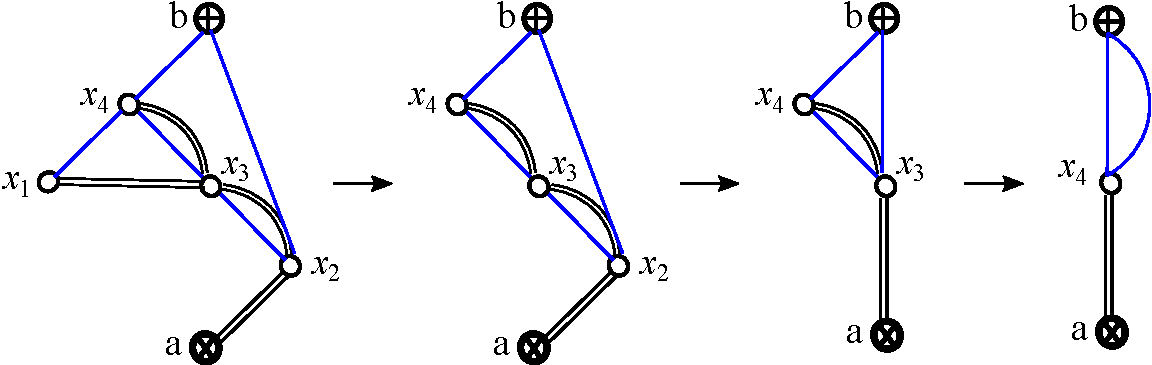
\includegraphics[width=10cm]{Graphreduction3.pdf}
\end{center}
Finally, we get a graph with only one internal atom $x_\ell$, one double-line edge between $\otimes$ and $x_\ell$, and two blue solid edges between $\oplus$ and $x_\ell$. Then using \eqref{Omega2}, we can bound \eqref{bound G aux} as
%Hence by counting the $W^{-d/2+\e_0}$ factors carefully, we can bound the first term in \eqref{Ho123} as
\begin{align*}
\cal G^{\rm abs}_{\fa,\fb\fb}\prec W^{-(n_{\cal G} -2)d/2+C_{\cal G}\e_0 + n_4\tau}\sum_{x_{\ell}}B_{\fa x_{\ell}}B_{ x_{\ell}\fb} \lesssim W^{-(n_{\cal G} -2)d/2+C_{\cal G}\e_0 + n_4\tau}\frac{L^2}{W^2} B_{\fa\fb} ,
\end{align*}
where we used a similar argument as in \eqref{calc1}, and we have renamed $C_{\cal G}$. Since $\tau$ is arbitrary, we can bound the first case in \eqref{Ho123} by the right-hand side of \eqref{ATab}. This concludes the proof.
\end{proof}
 
%\begin{proof} [Proof of Lemma \ref{no dot}]
	%	We first recall the definition of the normal regular graphs in Definition \ref{defnlvl0}. In particular, there are no dotted edges in $\cal G$, and each $G$ or $\overline G$ edge in $\cal G$ is off-diagonal.  
	%	%consider the special case where there are \emph{no dotted edges between different molecules} in $\cal G$. Later we will show that this special case easily extends to the more general case where there are dotted edges between different molecules.  
	%	By \eqref{sxyf}, \eqref{bandcw2}, \eqref{thetaxy} and \eqref{S+xy}, the following estimates hold:
	%	\be\label{Ssmall}\sum_{x} s_{xy} = 1 , \quad |s_{xy}| = \OO(W^{-d}), \quad \sum_{x} |S^{\pm}_{xy}|\lesssim 1 , \quad |S^{\pm}_{xy}|= \OO(W^{-d}),\ee
	%	and
	%	\be\label{Thetalarge}
	%	\sum_{x} \Theta_{xy} \sim \eta^{-1}, \quad |\Theta_{xy}| \prec W^{-d} .
	%	\ee
	%	%for any constant $\tau>0$. 
	%	%Together with \eqref{Gmax} and the definition \eqref{eq_deforderrandom2}, we can get the trivial bound
	%	%$$\left|(\cal G_0)_{xy}\right| \prec W^{(-d/2+\e_0)n_{xy}}\eta^{-k},$$
	%	%where $k$ is the number of sums over a single $\Theta$ edge out of all the summations over the atoms in $(\cal G_0)_{xy}$. 
	%	The $\eta^{-1}$ factor in the first equation is the main trouble we need to avoid. In the following proof, we will show that  if we choose the order of summation in a proper way, then the following key property holds: for every sum over a global scale $L$, it involves the product of at least one $\Theta$ edge with a variable satisfying the level-$(a,b)$ averaged or uniform bound for some $(a,b)$ satisfying \eqref{a+b}. In particular, every such summation does not provide a large $\eta^{-1}$ factor as we have seen in Claim \ref{cor: ini bound}.
	%	
	%	%Moreover, we will show that we can obtain a $W^{2} \langle x-y\rangle^{-(d+2)}$ factor after all the sums. 
	%	%Then checking the definition \eqref{eq_deforderrandom2}, we see that the main issue is the $\eta^{-1}$ factors coming from the summation over the $\Theta$ edges between different molecules.
	%	
	%	We first bound the local structures of $\cal G_{xy}$. For simplicity of notations, for two internal atoms $\al$ and $\beta$, we use $\al\sim_{\cal M} \beta$ to mean that ``$\al$ and $\beta$ belong to the same molecule". For each molecule, say $\cal M_i$, we choose any atom in it, say $x_i$, as a representative. In particular, let atoms $x$ and $y$ be the representatives of their respective molecules. Here for definiteness, we assume that $x$ and $y$ belong to \emph{different molecules}. The case where $\al$ and $\beta$ belong to the same molecule is similar, and we omit the relevant details.  %then we pick any of them as the representative. 
	%	
	%	For any $y_i\sim_{\cal M}x_i$, it suffices to assume that  
	%	\be\label{yixi}
	%	|y_i-x_i|\le (\log W)^2 W,
	%	\ee
	%	because otherwise the graph is smaller than $W^{-D}$ for any fixed $D>0$ by \eqref{compact f} and \eqref{S+xy}. Then for $y_i\sim_{\cal M} x_i$ and $y_j\sim_{\cal M} x_j$, by \eqref{Gpsi}, \eqref{thetaxy} and \eqref{yixi} we have that
	%	\be\label{intermole1}|G_{y_i y_j}|\prec \Psi_{x_i x_j} + \OO(W^{-D}),\quad \Theta_{y_i y_j}\prec B_{y_i y_j} \le (\log W)^{2d} B_{x_i x_j},\ee
	%	for any fixed $D>0$. Similarly, for any labelled $\dashed$ edge as in \eqref{eq label}, we have that %for any constant $\tau>0$, %$\Selek_{2l}\in \Cele_{2l}$,
	%	\be\label{intermole2} \left|(\Theta \Sele_{2k_1}\Theta  \Sele_{2k_2}\Theta \cdots \Theta  \Sele_{2k_l}\Theta)_{y_i y_j}\right| \prec W^{-(k/2-1)d } B_{x_i x_j} \ee 
	%	by \eqref{BRB}.
	%	%for any constant $\tau>0$. 
	%	%,\quad |(\Theta \Sele_{2l}\Theta)_{y_i y_j}| \le W^{-(l-1)d+\tau} B_{x_i x_j}.\ee
	%	We shall use \eqref{intermole1} and \eqref{intermole2} to bound the edges between different molecules, and all these bounds only involve the representative atoms $x_i$. Then it is easy to bound each local structure separately, i.e. the subgraph inside each molecule with a fixed representative atom. For the molecule $\cal M_i$ containing atom $x_i$, we bound the subgraph, say $\cal G_{x_i}^{(i)}$, inside $\cal M_i$ as follows: 
	%	\begin{itemize}
	%		\item we bound each waved edge and $\dashed$ edge by $\OO_\prec(W^{-d })$ using the $\ell^\infty$ bounds in \eqref{Ssmall}  and \eqref{Thetalarge}; 
	%		\item we bound each labelled $\dashed$ edge as in \eqref{eq label} by $\OO_\prec (W^{-kd/2 })$, where $k$ is the scaling order of this edge; %using \eqref{BRB}; 
	%		\item we bound each off-diagonal $G$ edge and light $G$ weight by $\OO_\prec(W^{-d/2})$ using the bound \eqref{eq PseudoG2} on $|G_{xy}(z)-m(z)\delta_{xy}|$; 
	%		\item we bound the summation over each internal atom in $\cal M_i \setminus \{x_i\}$ by $\OO((\log W)^{2d} W^d)$ due to \eqref{yixi}. 
	%	\end{itemize}
	%	Thus with the definition of the scaling order in \eqref{eq_deforderrandom3}, we get that
	%	\begin{align}\label{internal struc1}
	%		|\cal G_{x_i}^{(i)}|\prec W^{-\ord(\cal G^{(i)}_{x_i}) \cdot d/2} .
	%	\end{align} 
	%	%---x,y same molecule
	%	%As a special case, if $x$ and $y$ are in the same molecule, then for the subgraph inside this molecule, say $\wt {\cal G}_{xy}$, we bound it as
	%	% \begin{align}\label{internal struc2}
	%	%|\wt{\cal G}_{x y}|\prec  (W^{-d/2+\e_0})^{\ord(\wt{\cal G}_{xy})}\mathbf 1_{|x-y|\le (\log W)^2W}+ W^{-D} .
	%	%\end{align} 
	%	%----------------------------
	%	
	%	It remains to bound the global structure, that is, the edges between different molecules and the summations over the representative atoms. 
	%	%It remains to prove \eqref{bound 2net1}. 
	%	%Recall that every connected graph has a spanning tree. 
	%	%For the molecular graph, we can pick a black spanning tree from the black net with $\otimes$ as the root, and a blue spanning tree from the blue net with $\oplus$ as the root. 
	%	In the molecular graph of $\cal G_{xy}$, due to the doubly connected property we can pick two spanning trees for the blue net and the black net, which we shall call the \emph{blue tree} and \emph{black tree}, respectively. For the edges that do {\bf not} belong to the blue and black trees, we bound them using the $\ell^\infty$-bounds of \eqref{intermole1} and \eqref{intermole2}:
	%	\begin{itemize}
	%		\item for the $G$ and $\overline G$ edges that are not in the blue tree, we bound each of them by $\OO_\prec(\Psi_{x_i x_j} +  W^{-D})=\OO_\prec(W^{-d/2})$; 
	%		
	%		\item for the $\dashed$ $\Theta$ edges that are not in the blue and black trees, we bound each of them by $\OO_\prec(B_{x_i x_j})=\OO_\prec(W^{-d})$; 
	%		
	%		\item for the labelled $\dashed$ edges that are not in the blue and black trees, we bound each of them by $\OO_\prec(W^{-(k/2-1)d } B_{x_i x_j})=\OO_\prec(W^{-kd/2})$, where $k$ is the scaling order of this edge. 
	%	\end{itemize}
	%	On the other hand, for the $G$ edges and $\dashed$ edges in the blue and black trees, we use \eqref{intermole1} and \eqref{intermole2} to bound them. Moreover, 
	%	%More precisely, for a (labelled) $\dashed$ edges in the {\bf black} tree, we bound it as 
	%	%\be\label{bound thetaweak0} 
	%	%\begin{split}
	%	%&    \Theta_{y_i y_j}\prec  B_{x_i x_j}  ,\quad  \text{or} \quad \left|\left(\Theta \Sele_{2k_1}\Theta  \Sele_{2k_2}\Theta \cdots \Theta  \Sele_{2k_l}\Theta\right)_{y_i y_j}\right| \prec W^{-(k/2-1)d } B_{x_i x_j}, 
	%	%\end{split}
	%	%\ee
	%	for a labelled $\dashed$ edge in the {\bf blue} tree, we further bound it as 
	%	\be\label{bound thetaweak} 
	%	\Theta_{y_i y_j}\prec W^{-d/2}B_{x_i x_j} ^{1/2},\quad  \text{or}   \left|\left(\Theta \Sele_{2k_1}\Theta  \Sele_{2k_2}\Theta \cdots \Theta  \Sele_{2k_l}\Theta\right)_{y_i y_j}\right| \prec W^{-(k/2-1)d-d/2} B^{1/2}_{x_i x_j}, 
	%	\ee %\quad |(\Theta \Sele_{2l}\Theta)_{y_i y_j}| \prec W^{-(l-1)d-d/2} B^{1/2}_{x_i x_j},$$
	%	where $y_i\sim_{\cal M}x_i$ and $y_j\sim_{\cal M} x_j$, and $k$ is the scaling order of the labelled $\dashed$ edge.  In this way, up to some power of $W^{-d/2}$, every edge in the blue tree between the molecules $\cal M_i$ and $\cal M_j$ can be bounded by $B_{x_i x_j}^{1/2}$, which satisfies the level-$(1,1)$ uniform bound, or $\Psi_{x_i x_j} + \OO(W^{-D})$, which satisfies the level-$(1,3/2)$ averaged bound or the level-$(1,1)$ uniform bound depending on the assumptions. %while a $B^{1/2}_{x_i x_j}$ edge in the blue tree satisfies the level-$(1,1)$ uniform bound.
	%	
	%	
	%	Combining the above discussions, we can bound $\cal G_{xy}$ as
	%	\be\label{bound G aux}
	%	|\cal G_{xy}| \prec W^{- (n_{xy}-\ell -3) d/2} (\cal G_{xy})_{aux}.
	%	\ee
	%	where $\ell$ is the number of internal molecules in $\cal G_{xy}$ (excluding the external molecules containing $x$ or $y$), and $(\cal G_{xy})_{aux}$ is an auxiliary graph defined as follows: 
	%	\begin{itemize}
	%		\item we have two external atoms $x$ and $y$, and some internal atoms $x_i$, which are the representative atoms of the molecules in $\cal G_{xy}$; 
	%		
	%		\item each black edge in the black spanning tree between molecules $\cal M_i$ and $\cal M_j$ is replaced with a black $\dashed$ edge representing $B_{x_i x_j}$; 
	%		
	%		\item each blue edge in the blue spanning tree between molecules $\cal M_i$ and $\cal M_j$ is replaced with a blue solid edge representing a positive variable ($B_{x_i x_j}^{1/2}$ or $\Psi_{x_i x_j} + \OO(W^{-D})$) that satisfies the level-$(1,3/2)$ averaged bound or the stronger level-$(1,1)$ uniform bound . % (note that initially the pseudo $G$ variables are of the form $n^{-\e_0}\Psi_{x_i x_j}$ or $B^{1/2}_{x_i x_j}$). 
	%	\end{itemize}
	%	% Moreover, $\wt n_{xy}$ is defined as 
	%	% $$ \wt n_{xy}:= n_{xy} - \ell - 3 ,\quad \ell:=\#\{\text{internal atoms in } (\cal G_{xy})_{aux}\}  .$$
	%	% in order to match the scaling order $n_{xy}$ of the graph $\cal G_{xy}$. 
	%	Here the number $(n_{xy}-\ell -3)$ in the exponent can be obtained by counting the number of $W^{-d/2}$ factors from (i) the local structures \eqref{internal struc1}, (ii) the edges that are not in the black and blue tress, and (iii) the edges in the black and the blue tree.
	%	%can be obtained by counting the scaling order of all the components. 
	%	One can also get this number in the following simpler way.
	%	The auxiliary graph $(\cal G_{xy})_{aux}$ has scaling order $\ord((\cal G_{xy})_{aux})=\ell+ 3$, if we count it as 
	%	%where corresponding to \eqref{eq_deforderrandom2} we define
	%	\begin{align*}
	%		\ord((\cal G_{xy})_{aux}) &= \#\{\text{blue egdes}\}+2\#\{\text{black egdes}\}-2\#\{\text{internal atoms}\} \\
	%		&= (\ell+1) + 2(\ell + 1)-2\ell=\ell+3.
	%	\end{align*}
	%	Recall that $\cal G_{xy}$ has scaling order $n_{xy}$, so the difference is $n_{xy}-\ell -3.$ 
	%	%where the molecules are replaced with vertices in the graphs, the black edge (from the black spanning tree) between two vertices, say $\al$ and $\beta$, is replaced with a black $\dashed$ edge representing $B_{\al\beta}$, and the blue edge (from the blue spanning tree) between two vertices $\al$ and $\beta$ is replaced with a pseudo $G$ edge $\cal A_{\al\beta}$ as in Notation \ref{Def PseudoG}.
	%	%\be\label{sumpsi}
	%	%K^{-d} \max_w\sum_{|y-w|\le K} \Psi^2_{xy} \prec W^{2\e_0} \frac{1}{WK^{d/2-1}}
	%	%\ee
	%	
	%	Note that the graph $(\cal G_{xy})_{aux}$ is doubly connected in the following sense: it contains a black spanning tree consisting of black $\dashed$ edges only, and a blue spanning tree consisting of blue solid edges only, such that each of these two trees connects all atoms in $(\cal G_{xy})_{aux}$. 
	%	%which follows from the double-net structure of the original graph $\cal G_{xy}$.
	%	Now with \eqref{bound G aux}, to conclude the proof it suffices to show that after summing over all the internal atoms in $ (\cal G_{xy})_{aux}$, the auxiliary graph can be bounded by
	%	\be\label{boundaux0}
	%	| (\cal G_{xy})_{aux}| \prec W^{-\ell d/2  }B_{xy}\cal A_{xy} ,
	%	\ee
	%	%for some pseudo $G$ variable $\cal A_{xy}$. 
	%	where $\cal A_{xy}$ is a positive variable satisfying the level-$(1,3/2)$ averaged bound (resp.  level-$(1,1)$ uniform bound) if $|G_{xy}(z)-m(z)\delta_{xy}|$ satisfies the level-$(1,3/2)$ averaged bound  (resp.  level-$(1,1)$ uniform bound). This estimate \eqref{boundaux0} is an easy consequence of the following more general claim. We postpone the proof of this claim until we complete the proof of Lemma \ref{no dot}.
	%	
	%	\begin{claim}\label{twonet claim}
	%		Let $ (\cal G_{xy})_{aux}$ be an auxiliary graph as above. In other words, $ (\cal G_{xy})_{aux}$ has two external atoms $x$ and $y$, $\ell$ internal atoms $x_1, x_2,\cdots, x_\ell$, a black spanning tree consisting $(\ell+1)$ black edges, and a blue spanning tree consisting $(\ell+1)$ blue edges. Moreover, suppose each black edge between atoms, say $\al$ and $\beta$, represents a $B_{\al\beta}$ factor, and each blue edge represents a positive variable satisfying the level-$(a,b)$ averaged bound. If \eqref{a+b} holds, then we have 
	%		\be\label{boundaux}
	%		| (\cal G_{xy})_{aux}| \prec W^{-a\ell  d /2  }B_{xy}\cal A_{xy} ,
	%		\ee
	%		where $\cal A_{xy}$ is a positive variable satisfying the level-$(a,b)$ averaged bound. 
	%		Moreover, if each blue edge represents a positive variable satisfying the level-$(a,b)$ uniform bound and \eqref{a+b} holds, then $\cal A_{xy}$ is a positive variable satisfying the level-$(a,b)$ uniform bound. 
	%	\end{claim}
	%	Note that both $(a,b)=(1,3/2)$ and $(a,b)=(1,1)$ satisfy \eqref{a+b}. Hence taking $a=1$ in \eqref{boundaux}, we obtain \eqref{boundaux0}. Now combining \eqref{bound G aux} and \eqref{boundaux0}, we conclude \eqref{bound 2net1} and \eqref{bound 2net1 strong}. 
	%	Finally, in the above proof, we have only used the bounds on the absolute values of the components in $\cal G_{xy}$, hence the last statement on $\cal G^{\rm{abs}}_{xy}$ holds.
	%	%Next we consider the general case where there are dotted edges between different molecules. In this case, we combine all the atoms in $\cal G_{xy}$ that are connected through dotted edges, and obtain a reduced graph. It is easy to check that this reduced graph is still doubly connected and has no dotted edges between different molecules. Hence we are reduced to the previous setting again. 
	%	%  Finally, if $G$ satisfies the sharp estimate \eqref{locallaw}, then all the off-diagonal 
	%	%$G_{\al\beta}$ edges in $\cal G$ can be bounded by $B^{1/2}_{\al\beta}$. Then the 
	%	% above proof still holds if we replace all pseudo $G$ variables $\cal A_{\al\beta}$ with $B^{1/2}_{\al\beta}$, which gives \eqref{bound 2net1 strong}.
	%\end{proof}
%		\iffalse	
%	\begin{proof}[Proof of Claim \ref{twonet claim}]
%
%		Our proof is based on the following extension of the estimate in Claim \ref{cor: ini bound}. If $\cal A^{(1)}$ and $\cal A^{(2)}$ are two matrices satisfying the level-$(a,b)$ averaged (resp. uniform) bound, then %we have that 
%		\be%\label{keyobs}
%		\begin{split}
%			& {\cal A}_{\al\beta}:=\frac{W^{ad/2 }}{\Gamma(y_1,\cdots, y_k)}\sum_{x_i} B_{y_1 x_i}\cdots B_{y_k x_i}\cal A^{(1)}_{x_i \al}\cal A ^{(2)}_{x_i \beta} \ \ \text{satisfies the }\\
%			& \text{level-$(a,b)$ averaged (resp. uniform) bound,}
%		\end{split}
%		\ee
%		where $\Gamma(y_1,\cdots, y_k)$ is a sum of different products of $(k-1)$ black $B$ edges:  
%		\be%\label{defn_Gamma}
%		\Gamma(y_1,\cdots, y_k):= \sum_{i=1}^k \prod_{j\ne i}B_{y_{i}y_j}.\ee
%		\eqref{keyobs} can be reformulated into a clearer form:
%		\be%\label{keyobs2}
%		\sum_{x_i} B_{y_1 x_i}\cdots B_{y_k x_i}\cal A^{(1)}_{x_i \al}\cal A^{(2)} _{x_i \beta}  \le W^{-a d/2 }\Gamma(y_1,\cdots, y_k)  {\cal A}_{\al\beta},
%		\ee
%		for a variable $ {\cal A}_{\al\beta}$ satisfying the same type of bound as $\cal A^{(1)}_{x_i \al}$ and $\cal A^{(2)} _{x_i \beta}$. Intuitively speaking, after the summation over a product of $k$ black edges and 2 blue edges, we lose one black edge and one blue edge, which give rise to the $W^{-ad/2 }$ factor as in Claim \ref{cor: ini bound}. In the new graph, we have $(k-1)$ black edges connected with one of the neighbors of $x_i$ on the black tree and one pseudo $G$ edge between atoms $\al$ and $\beta$. 
%		
%		
%		In the following example, we draw an example with $k=3$, where there are three graphs corresponding to the term on the right-hand side of \eqref{keyobs2}. 
%		%Here we lose one $B$ edge and one pseudo $G$ edge, which give rise to the $W^{-d/2 }$ factor after summation as in Lemma  \ref{cor: ini bound}. 
%		\begin{center}
%			\includegraphics[width=7cm]{sumbedges.png}
%		\end{center}
%		
%		
%		We first prove \eqref{keyobs} when $\cal A^{(1)}$ and $\cal A^{(2)}$ satisfy the level-$(a,b)$ averaged bound. For this purpose, we first show the following bound:
%		\be%\label{keyobs3}
%		\sum_{x_i} B_{y_1 x_i}\cdots B_{y_k x_i}\cal A^{(2)}_{x_i \beta}\prec W^{-ad/2 } \Gamma(y_1,\cdots, y_k).
%		\ee
%		We decompose the sum over $x_i$ according to dyadic scales $K_n$ defined in \eqref{defn Kn}. Consider the case $x_i \in \cal I_{\vec a}$ for some $\vec a:=(a_1, \cdots, a_k)\in (\N\setminus\{0\})^k$, where 
%		$$\cal I_{\vec a}:=\{ x_i: K_{a_j-1} \le |x_i - y_j| \le K_{a_j} ,  1\le j \le k\}.$$ For simplicity of notations, we abbreviate $L_j := K_{a_j}$ and $L_{\min}:=\min_{1\le j \le k}L_j $. Then we obtain that 
%		\begin{align}\label{sum_ba}
%			\sum_{x_i \in \cal I_{\vec a}} B_{y_1 x_i}\cdots B_{y_k x_i}\cal A ^{(2)}_{x_i \beta} \le \prod_{j=1}^k\frac{1}{W^2L_j^{d-2}} \sum_{x_i\in \cal I_{\vec a}}  \cal A ^{(2)}_{x_i \beta}  \prec   \frac{L_{\min}^{d}}{W^bL_{\min}^{ad/2-b} }\frac{1}{\prod_{j=1}^k W^2L_j^{d-2}} ,  
%		\end{align}  
%		where in the second step we used \eqref{eq PseudoG} and the fact that $\cal I_{\vec a}$ is inside a box of scale $L_{\min}$.
%		%\begin{align}
%		% K^{-d}\sum_{\al: |\al- w|\le K}\sum_{x_i \in \cal I_{\vec a}} B_{y_1 x_i}\cdots B_{y_k x_i}\cal A_{x_i \al}\cal A _{x_i \beta} &\prec \frac{1}{W^{1/2}K^{d/4-1/2}} \prod_{j=1}^k\frac{1}{W^2L_j^{d-2}} \sum_{x_i\in \cal I_{\vec a}}  \cal A _{x_i \beta} \label{verifypseudo1}\\
%		%&\prec  \frac{1}{W^{1/2}K^{d/4-1/2}}  \frac{(L_1\wedge L_2\wedge \cdots \wedge L_k)^{3d/4+1/2}W^{-1/2}}{\prod_{j=1}^k W^2L_j^{d-2}} . \nonumber
%		%\end{align}  
%		Let $s$ be a number such that $L_s=L_{\min}$. Using \eqref{a+b}, we obtain that
%		$$\frac{L_{\min}^{d}}{ W^b L_{\min}^{ad/2-b} } \frac1{W^2L_s^{d-2}} \le \frac{1}{W^{b+2}L_{\min}^{ad/2-b-2}}\le W^{-ad/2}.$$
%		Together with the fact that for all $j\ne s$, 
%		\be\label{yj-s}\langle y_j - y_s \rangle \le W+ L_j + L_s \le 3L_j,\ee  
%		we can bound \eqref{sum_ba} as 
%		\begin{align}
%			\sum_{x_i \in \cal I_{\vec a}} B_{y_1 x_i}\cdots B_{y_k x_i}\cal A ^{(2)}_{x_i \beta} \prec W^{-ad/2} \prod_{j\ne s} \frac1{W^2L_j^{d-2}} \lesssim W^{-ad/2} \prod_{j\ne s} B_{y_j y_s} \le  W^{-ad/2}{\Gamma(y_1,\cdots, y_k)} . \nonumber
%		\end{align}  
%		Summing over all possible scales $\cal I_{\vec a}$, we conclude \eqref{keyobs3}.
%		% \begin{align*}
%		%\sum_{x_i} B_{y_1 x_i}\cdots B_{y_k x_i}\cal A_{x_i \beta} \prec  W^{-d/2} {\Gamma(y_1,\cdots, y_k)} , %\label{checkpseudo1}
%		%\end{align*}  
%		%which concludes \eqref{keyobs3}.
%		%In order to improve the $W^{-d/4+\e_0}$ factor to $W^{-d/2+\e_0}$, we again can use the arguments in Corollary \ref{cor: ini bound}. 
%		%This concludes \eqref{eq PseudoG} for $\wt A_{\al\beta}$. 
%		%\begin{align*}
%		%&\sum_{x_i \in \cal I_{\vec a}} B_{y_1 x_i}\cdots B_{y_k x_i}\cal A_{x_i \al}\cal A _{x_i \beta} \prec  \sum_{x_i\in \cal I_{\vec a}} B_{y_1 x_i}\cdots B_{y_k x_i}\cal A_{x_i \al}(B^{1/2}_{x_i \beta}+\wt\Phi) \\
%		%&\prec W^{\e_0}\frac{(L_1\wedge L_2\wedge \cdots \wedge L_k)^{3d/4+1/2}W^{-1/2}}{\prod_{j=1}^k W^2L_j^{d-2}} (B^{1/2}_{\al \beta}+\wt\Phi) \prec W^{-d/4+\e_0}\Gamma(y_1,\cdots, y_k)(B^{1/2}_{\al \beta}+\wt\Phi),
%		%\end{align*}
%		%where in the second and third steps we used similar arguments as in the proof for \eqref{checkpseudo1}. Again using the arguments in Corollary \ref{cor: ini bound}, we can improve the $W^{-d/4+\e_0}$ factor to $W^{-d/2+\e_0}$. This concludes \eqref{eq PseudoG2} for $\wt A_{\al\beta}$. 
%		%In sum, we have proved \eqref{keyobs} and \eqref{keyobs2}. 
%		%which can be stated in the more convenient form: 
%		%\be\label{keyobs2}
%		%\sum_{x_i} B_{y_1 x_i}\cdots B_{y_k x_i}\cal A_{x_i \al}\cal A _{x_i \beta} =W^{-d/2+\e_0} \Gamma(y_1,\cdots, y_k)\AIT_{\al\beta},
%		%\ee
%		%for a pseudo $G$ edge $\AIT_{\al\beta}$. 
%		Now applying \eqref{eq PseudoG2} to $\cal A^{(1)}_{x_i\al}$ and using \eqref{keyobs3}, we get that
%		\begin{align*}
%			&\sum_{x_i } B_{y_1 x_i}\cdots B_{y_k x_i}\cal A^{(1)}_{x_i \al}\cal A ^{(2)}_{x_i \beta} \prec W^{-ad/2}\sum_{x_i } B_{y_1 x_i}\cdots B_{y_k x_i}\cal A^{(2)}_{x_i \beta}   \prec W^{-ad }\Gamma(y_1,\cdots, y_k),
%		\end{align*}
%		Applying \eqref{eq PseudoG} to $\cal A^{(1)}_{x_i\al}$ and using \eqref{keyobs3}, we get that for any $w\in Z_L^d$ and $ W\le K \le L$,
%		\begin{align*}
%			K^{-d}\sum_{\al: |\al- w|\le K}\sum_{x_i  } B_{y_1 x_i}\cdots B_{y_k x_i}\cal A^{(1)}_{x_i \al}\cal A ^{(2)}_{x_i \beta}& \prec \frac{\sum_{x_i } B_{y_1 x_i}\cdots B_{y_k x_i}\cal A_{x_i \beta}}{W^{b}K^{ad/2-b}}  \prec W^{-ad/2} \frac{\Gamma(y_1,\cdots, y_k)}{W^{b}K^{ad/2-b}}. 
%		\end{align*}  
%		The above two estimates imply that \eqref{eq PseudoG2} and \eqref{eq PseudoG} hold for $\cal A_{\al\beta}$, i.e. it satisfies the level-$(a,b)$ averaged bound. %which concludes \eqref{keyobs}.
%		
%		
%		Next we prove \eqref{keyobs} when $\cal A^{(1)}$ and $\cal A^{(2)}$ satisfy the level-$(a,b)$ uniform bound. We decompose the sum over $x_i$ according to dyadic scales: $x_i \in \cal I_{\vec a}$ for some $\vec a:=(a_1, \cdots, a_{k+2})\in (\N\setminus\{0\})^{k+2}$, where 
%		$$\cal I_{\vec a}:=\{ x_i: K_{a_j-1} \le |x_i - y_j| \le K_{a_j} ,  1\le j \le k, K_{a_{k+1}-1} \le |x_i-\al|\le K_{a_{k+1}}, K_{a_{k+2}-1} \le |x_i-\beta|\le K_{a_{k+2}}\}.$$ For simplicity of notations, we abbreviate $L_j := K_{a_j}$, $1\le j \le k+2$, and $L_{\min}:=\min_{1\le j \le k}L_j$. Again let $j$ be a number such that $L_j=L_{\min}$. Then using \eqref{eq unifG} and that $\cal I_{\vec a}$ is inside a box of scale $L_{\min}\wedge L_{k+1}\wedge L_{k+2}$, we obtain that 
%		\begin{align} \nonumber
%			\sum_{x_i \in \cal I_{\vec a}} B_{y_1 x_i}\cdots B_{y_k x_i}\cal A ^{(1)}_{x_i \al} \cal A ^{(2)}_{x_i \beta} & \prec \prod_{j=1}^k\frac{1}{W^2L_j^{d-2}} \cdot\frac{(L_{\min}\wedge L_{k+1}\wedge L_{k+2})^d}{W^{2b} L_{k+1}^{ad/2-b}L_{k+2}^{ad/2-b}} \\
%			&\le   \prod_{1\le j \le k, j\ne s}\frac{1}{W^2L_j^{d-2}} \cdot\frac{1}{W^{b} (L_{k+1}\vee L_{k+2})^{ad/2-b}}\cdot\frac{1}{W^{b+2}L_{\min}^{ad/2-b-2}} \nonumber\\
%			& \le W^{-ad/2} \frac{1}{W^{b} \langle \al-\beta \rangle^{ad/2-b}}\prod_{j\ne s} B_{y_j y_s}. \nonumber
%		\end{align}  
%		In the above derivation, we used $L_{k+1} L_{k+2}=(L_{k+1}\vee L_{k+2})(L_{k+1}\wedge L_{k+2})$ in the second step, and \eqref{a+b}, \eqref{yj-s} and  $\langle \al - \beta \rangle \le W+ L_{k+1} + L_{k+2} \le 3L_{k+1}\vee L_{k+2} $ in the last step. The estimate implies that \eqref{eq unifG} holds for $\cal A_{\al\beta}$, i.e. it satisfies the level-$(a,b)$ uniform bound. This concludes \eqref{keyobs} together with the above proof for the averaged bound.
%		
%		%With the above observations, we can finally sum over the molecules on this path from $\cal M_{k_0}$ to $\cal M_b$ and conclude the proof.
%	
%		
%		
%		Then the proof of \eqref{boundaux} involves repeated applications of  \eqref{keyobs2} and \eqref{keyobs3} with a carefully chosen order of summations. Without loss of generality, we regard $y$ as the root of the blue tree, and sum over the vertices from the leaves of the blue tree to the root $y$ except for the vertex $x$. More precisely, we will sum over the vertices according to a partial order $x_{i_1}\preceq x_{i_2} \preceq \cdots \preceq x_{i_\ell}\preceq y$ that is compatible with the blue tree structure: if $x_i$ is a child of $x_j$, then we have $x_i \preceq x_j$. Here $i_1,\cdots, i_\ell$ is a permutation of $1,\cdots, \ell$.  Without loss of generality, in the following proof we assume that the partial order is $x_1\preceq x_2  \preceq\cdots \preceq x_\ell$, so that we will perform the sum according to the order $\sum_{x_\ell}\cdots \sum_{x_2}\sum_{x_1}$. For simplicity of notations, we denote all the solid blue edges appearing in the proof by $\cal A$, including the original edges in  $(\cal G_{xy})_{aux}$ and the new edges coming from applications of \eqref{keyobs}. All these $\cal A$ variables satisfy the level-$(a,b)$ averaged or uniform bound, and their exact forms may change from one line to another. 
%		
%		For the sum over $x_1$, using \eqref{keyobs2} (if $x_1$ is connected with $x$ in the blue tree) or \eqref{keyobs3} (if  $x_1$ is not connected with $x$ in the blue tree), we can bound $ (\cal G_{xy})_{aux}$ as
%		\be\label{reduceaux1}(\cal G_{xy})_{aux} \prec W^{-ad/2 }\sum_{k=1}^{n_1} (\cal G^{(1)}_{xy,k})_{aux},\ee
%		where $(\cal G^{(1)}_{xy, k})_{aux}$ are the auxiliary graphs obtained by replacing the edges connected to $x_1$ with the graphs on the right-hand side of \eqref{keyobs2} or \eqref{keyobs3}, and $n_1$ is the number of neighbors of $x_1$ on the black tree. More precisely speaking, after summing over $x_1$, we get rid of the solid blue edge connected with $x_1$. If $x$ and $x_1$ are connected through a blue edge in $(\cal G_{xy})_{aux} $, then in each new graph $x$ is connected to the parent of $x_1$ on the blue tree through a blue edge. Moreover, Suppose $w_{1},\cdots,w_{n_1}$ are the neighbors of $x_1$ on the black tree. Then corresponding to the $n_1$ terms in $\Gamma(w_{1},\cdots, w_{n_1})$, the atoms $w_{1},\cdots,w_{n_1}$ are now connected to one of them, say $w_{k}$, through black edges in the new graphs, which give the $n_1$ different choices in \eqref{reduceaux1}. Now it is crucial to observe that each new graph $(\cal G^{(1)}_{xy,k})_{aux}$ is still doubly connected, that is, there are separated blue and black trees, each of which connects all the atoms $x,y, x_2,\cdots, x_\ell$. 
%		
%		Then we sum over the atoms $x_2, \cdots , x_{\ell}$ one by one and use \eqref{keyobs2} or \eqref{keyobs3} repeatedly: at each step we gain an extra factor $W^{-ad/2}$ and reduce the graph into the sum of several new graphs, each of which has one fewer atom and  a doubly connected structure. Finally, after summing over all internal atoms, we obtain a graph with atoms $x$ and $y$ only, and the only doubly connected graph is the graph where $x$ and $y$ are connected with a black $B$ edge and a solid blue edge that represents a variable $\cal A_{xy}$ satisfying the level-$(a,b)$ averaged or uniform bound. This concludes \eqref{boundaux}. 
%		
%	
%		In \eqref{Graphreduction}, we show the way to reduce the first graph to the second one through a sum over $x_1$.
%		%\begin{center}
%		\be  \label{Graphreduction}
%		\parbox[c]{0.9\linewidth}{\includegraphics[width=\linewidth]{Graphreduction2.png}} 
%		\ee
%		In \eqref{Graphreduction} we give an example of all possible graph reductions by summing over the 5 internal atoms. 
%		%\end{center}
%
%		%In the end, 
%		%$$(\cal G_{xy})_{aux} \prec W^{-ad\ell /2}B_{xy}\cal A_{xy}.$$
%		%This proves \eqref{boundaux}, which further concludes \eqref{bound 2net1}.  
%	\end{proof}
%	
%	%\iffalse
%	%\begin{remark}
%	%We only combine the molecules for the purpose of this proof. In the graph expansions, we generally keep the dotted edges and do not combine different molecules in order to keep track of the graph structure in a clearer way. %in some unwanted way. %(\cor will rethink about this\nc). 
%	%\end{remark}
%	%\fi
%	
%	
%	%\begin{corollary}\label{order cor}
%	%Given a graph with dashed black $b^{(1)}$ edges and solid blue $G$ edges, if we can use (some of the) blue edges to build an oriented tree that connects all the molecules, then Theorem \ref{order thm} holds. As a special case, Theorem \ref{order thm} holds if there exists a blue edge path that connects all the molecules.
%	%\end{corollary}
%	%
%	%\begin{proof}
%	%The second statement is a special case of the first one, because a path is a 1-regular tree. Now we prove the first statement. We only need to prove that \eqref{order eq} holds. 
%	%
%	%We define the depth of a molecule as its graph distance to the root. Let $L$ be the depth of the tree (i.e. the depth of the deepest molecule). Then we define an order ``$<$" of the molecules in the following way. For the molecules with different depth, we have
%	%$$\cal M_i < \cal M_j \quad \text{if} \quad \text{depth}(\cal M_i) > \text{depth}(\cal M_j) .$$
%	%For the molecules with the same depth, we fix an arbitrary order of them. Let $\pi$ be such that $\cal M_{\pi(1)} < \cal M_{\pi(2)} < \cdots < \cal M_{\pi(n)}$, then we have \eqref{order eq} holds because for any molecule $\cal M_{\pi(i)}$, it is connected to its parent $\cal M_{\pi(t)}$ through a blue edge. By definition of the order, we have $t>s$. 
%	%\end{proof}
%\fi
 

\begin{proof}[Proof of Lemma \ref{lem hook}]
We follow the proof of Claim \ref{lem ATab} (iii). Since we only use upper bounds on the absolute values of the components of $\cal G$ that follow from \eqref{G entry}, the last statement of Lemma \ref{lem hook} follows from the same proof. Let $\al$ be an internal atom of $\cal G$ and $c\in\Z_L^d$, and let $x_w$ be the representative atom of the molecule containing $\al$. By \eqref{yixi}, we have $B^{1/2}_{c\al}\lesssim W^{(d-2)\tau/4}B^{1/2}_{cx_w}$ up to a negligible error $\OO(W^{-D})$. Hence, applying the arguments between \eqref{Ssmall} and \eqref{bound G aux} to all forms in \eqref{Ho123} (including the second and third forms, which were bounded using Lemma \ref{no dot} in the proof of Claim \ref{lem ATab}), we obtain that
\be\label{hook aux0}
\cal G^{\rm abs}[\al;c]_{\fa,\fb\fb}\prec W^{-(n_{\cal G}-\ell-1)d/2+C_{\cal G}\e_0+n_4\tau}\, (\cal G_{\fa\fb})_{aux}[x_w;c],
\ee
where $(\cal G_{\fa\fb})_{aux}[x_w;c]$ is obtained by adding the factor $B^{1/2}_{cx_w}$ to an auxiliary graph $(\cal G_{\fa\fb})_{aux}$ satisfying the properties listed below \eqref{bound G aux}. (For the second and third forms in \eqref{Ho123}, the two blue solid edges connected with $\oplus$ end at the same internal atom, or $\oplus$ is connected to an internal atom through a double-line edge instead.) By \eqref{Omega2}, every blue solid edge between atoms $x$ and $y$ in the auxiliary graph is bounded by $W^{\e_0+\tau}B_{xy}^{1/2}$.

To estimate the auxiliary graph, we introduce the following positive matrices:
\be\label{FVJ}
F_{xy}:=\left(\frac{\langle x-y\rangle}{W}\right)^{-(d-2)}=W^d B_{xy},\qquad V_{xy}:=F_{xy}^{1/2},\qquad J_{xy}:=F_{xy}^{3/2}.
\ee
Let $\cal T_{\rm b}$ and $\cal T_{\rm u}$ be the black and blue spanning trees on the internal atoms $x_1,\ldots, x_\ell$ in the auxiliary graph, let $x_{i_0}$ be the internal atom connected to $\otimes$, and let $x_{j_1}$ and $x_{j_2}$ be the internal atoms connected to $\oplus$ through the two blue solid edges. (If $\oplus$ is connected to $x_{j_1}$ through a double-line edge instead, then we take $x_{j_2}=x_{j_1}$ in the following argument, since $B_{x\fb}=W^{-d}V_{x\fb}^2$ with $V$ defined in \eqref{FVJ} below.) There are $\ell$ double-line edges and $\ell+1$ blue solid edges in the auxiliary graph, and we sum over $\ell$ internal atoms. Hence, writing $B=W^{-d}F$ and $B^{1/2}=W^{-d/2}V$, we obtain that
\be\label{hook aux1}
(\cal G_{\fa\fb})_{aux}[x_w;c]\prec W^{(\ell+1)\e_0}\,W^{-(\ell+1)d/2}\,W^{-d/2}\,\cal I,
\ee
where
$$\cal I:=W^{-\ell d}\sum_{x_1,\ldots,x_\ell}F_{\fa x_{i_0}}\prod_{(x_i,x_j)\in \cal T_{\rm b}}F_{x_ix_j}\prod_{(x_i,x_j)\in \cal T_{\rm u}}V_{x_ix_j}\cdot V_{x_{j_1}\fb}V_{x_{j_2}\fb}\cdot V_{cx_w}.$$
We claim that
\be\label{hook I}
\cal I\le C F_{\fa\fb}
\ee
for a constant $C$ depending only on $d$ and $\ell$. Combining \eqref{hook aux0}, \eqref{hook aux1} and \eqref{hook I}, we obtain that
$$\cal G^{\rm abs}[\al;c]_{\fa,\fb\fb}\prec W^{C_{\cal G}\e_0+n_4\tau}\,W^{-n_{\cal G}d/2}\,W^{-d/2}F_{\fa\fb}=W^{C_{\cal G}\e_0+n_4\tau}\,W^{-(n_{\cal G}-2)d/2}\,W^{-d/2}B_{\fa\fb},$$
where we have renamed $C_{\cal G}$. Since $\tau$ is arbitrary, this concludes \eqref{hook bound}.

To prove \eqref{hook I}, we first collect some simple estimates. Since $d>6$, we have $j_0:=3(d-2)/2>d$, so
\be\label{J summable}
\max_x W^{-d}\sum_t J_{xt}\le C,\qquad \max_{u,c}W^{-d}\sum_t F_{ut}V_{ct}\le C,
\ee
where the second bound follows from H\"older's inequality
$$W^{-d}\sum_tF_{ut}V_{ct}\le \Big(W^{-d}\sum_tF_{ut}^{3/2}\Big)^{2/3}\Big(W^{-d}\sum_tV_{ct}^3\Big)^{1/3}$$
and $F^{3/2}=V^3=J$. Moreover, for any exponent $0<e\le j_0$, we have that
\be\label{conv J}
W^{-d}\sum_t J_{xt}\left(\frac{\langle t-y\rangle}{W}\right)^{-e}\le C\left(\frac{\langle x-y\rangle}{W}\right)^{-e}.
\ee
To see this, we denote $r:=\langle x-y\rangle/W$. On the region $\{t:|t-y|\ge |x-y|/2\}$, we have $\langle t-y\rangle/W\ge r/2$, and we use the first bound in \eqref{J summable}. On the region $\{t:|t-y|<|x-y|/2\}$, we have $|x-t|>|x-y|/2$, so $J_{xt}\le 2^{j_0}r^{-j_0}$, while
$$W^{-d}\sum_{t:|t-y|<|x-y|/2}\left(\frac{\langle t-y\rangle}{W}\right)^{-e}\le C g_e(r),\qquad g_e(r):=\begin{cases}r^{d-e}, & e<d,\\ 1+\log r, & e=d,\\ 1, & e>d.\end{cases}$$
Since $r\ge 1$, $j_0>d$ and $e\le j_0$, we have $r^{-j_0}g_e(r)\le Cr^{-e}$ in all three cases, which concludes \eqref{conv J}. Taking $e=j_0$, $d-2$ and $(d-2)/2$ in \eqref{conv J}, we get that
\be\label{conv JFV}
W^{-d}\sum_t J_{xt}J_{ty}\le CJ_{xy},\quad W^{-d}\sum_t J_{xt}F_{ty}\le CF_{xy},\quad W^{-d}\sum_t J_{xt}V_{ty}\le CV_{xy}.
\ee
Finally, since $\langle \fa-\fb\rangle\le 2\max\{\langle \fa-t\rangle,\langle t-\fb\rangle\}$, we have $\min\{F_{\fa t},F_{t\fb}\}\le 2^{d-2}F_{\fa\fb}$, so $F_{\fa t}F_{t\fb}\le 2^{d-2}F_{\fa\fb}(F_{\fa t}+F_{t\fb})$. Together with the second bound in \eqref{J summable}, it gives that
\be\label{three point}
W^{-d}\sum_t F_{\fa t}F_{t\fb}V_{ct}\le CF_{\fa\fb},\quad \text{uniformly in }c\in \Z_L^d.
\ee

Now we prove \eqref{hook I}. By the weighted AM-GM inequality $s^{2/3}u^{1/3}\le \frac23 s+\frac13 u$ for $s,u\ge 0$, and the identities $F=J^{2/3}$, $V=J^{1/3}$, we have
\be\label{amgm}
\prod_{(x_i,x_j)\in \cal T_{\rm b}}F_{x_ix_j}\prod_{(x_i,x_j)\in \cal T_{\rm u}}V_{x_ix_j}\le \frac23\prod_{(x_i,x_j)\in \cal T_{\rm b}}J_{x_ix_j}+\frac13\prod_{(x_i,x_j)\in \cal T_{\rm u}}J_{x_ix_j}.
\ee
Moreover, we have $V_{x_{j_1}\fb}V_{x_{j_2}\fb}\le (F_{x_{j_1}\fb}+F_{x_{j_2}\fb})/2$. Hence it suffices to show that for any spanning tree $\cal T$ on the atoms $x_1,\ldots,x_\ell$ and any $i_0,j,w\in\{1,\ldots,\ell\}$,
\be\label{hook I2}
W^{-\ell d}\sum_{x_1,\ldots,x_\ell}F_{\fa x_{i_0}}F_{x_j\fb}V_{cx_w}\prod_{(x_i,x_k)\in\cal T}J_{x_ix_k}\le CF_{\fa\fb}.
\ee
To prove \eqref{hook I2}, we first sum over the leaves of $\cal T$ that do not belong to $\{x_{i_0},x_j,x_w\}$ one by one using the first bound in \eqref{J summable}, until we get the minimal subtree $\cal T'$ of $\cal T$ containing $x_{i_0}$, $x_j$ and $x_w$. There is a unique atom $x_t$ in $\cal T'$ (which may coincide with some of $x_{i_0}$, $x_j$ and $x_w$) such that $\cal T'$ is the union of the three paths from $x_{i_0}$, $x_j$ and $x_w$ to $x_t$, which are disjoint except at $x_t$. We sum over the atoms on the path from $x_{i_0}$ to $x_t$ (excluding $x_t$) one by one starting from $x_{i_0}$, using the second bound in \eqref{conv JFV} at each step. This replaces $F_{\fa x_{i_0}}$ with $CF_{\fa x_t}$. In the same way, we replace $F_{x_j\fb}$ with $CF_{x_t\fb}$, and $V_{cx_w}$ with $CV_{cx_t}$ using the third bound in \eqref{conv JFV}. Finally, we sum over $x_t$ using \eqref{three point}, which concludes \eqref{hook I2}, and hence \eqref{hook I}.
\end{proof}

\subsection{Proof of Lemma \ref{eta1case0}}\label{sec eta1}
In this subsection, we prove Lemma \ref{eta1case0} with a high moment argument based on the second order $T$-expansion \eqref{seconduniversal}.
%\begin{proof}[Proof of Lemma \ref{eta1case0}]
In the $\eta=1$ case,
%we have $|m(z)|\le 1 - \al$ for some constant $\al>0$, which gives
%$$\sum_x \Theta_{xy} = \frac{|m(z)|^2}{1-|m(z)|^2}=\OO(1).$$
 by \eqref{thetaxy} we have that for any small constant $\tau>0$ and large constant $D>0$,
 \be\label{thetaxy eta1}\Theta_{xy}\le \frac{W^\tau}{W^d}\mathbf 1_{|x-y|\le W^{1+\tau}}+ \OO(W^{-D}).\ee
%that is, $\Theta_{xy}$ is negligible when $|x-y|\gg W$.
In other words, the $\Theta$ edge is typically a ``short edge" of length $\OO_\prec(W)$. Moreover, the following local law on $G(z)$ was proved in \cite{ErdYauYin2012Univ,Semicircle}.
\begin{lemma}[Theorem 2.3 of \cite{Semicircle} and Theorem 2.1 of \cite{ErdYauYin2012Univ}]\label{semicircle}
Suppose the assumptions of Theorem \ref{main thm} hold. For any constants $\kappa, \e >0$, the local law
\be\label{jxw}
\max_{x,y}|G_{xy}(z) - \delta_{xy}m(z)| \prec ( W^d\eta)^{-1/2}
 \ee
 holds uniformly in $z=E+\ii \eta$ with $E\in (-2+\kappa, 2- \kappa)$ and $\eta \in[W^{-d+\e},1]$.
\end{lemma}

Lemma \ref{semicircle} will only be used at $\eta=1$, and in this case \eqref{jxw} can also be proved directly without \cite{ErdYauYin2012Univ,Semicircle}: since $\|G\|\le \eta^{-1}=1$, we have $\sum_{u}|G^{(x)}_{uy}|^2\le 1$ for all $x,y$, so the Schur complement formulas \eqref{schur} and the large deviation estimates in Lemma \ref{lem gauss} below give $|G_{xy}|\prec W^{-d/2}|G_{xx}|$ for $x\ne y$ and $G_{xx}-m=mG_{xx}[\sum_u s_{xu}(G_{uu}-m)+\OO_\prec(W^{-d/2})]$, which implies $\max_x|G_{xx}-m|\prec W^{-d/2}$ because $|G_{xx}|\le 1$ and $|m(E+\ii)|\le 0.62$.

With \eqref{jxw} as the a priori estimate, we prove a high moment estimate on the $T$-variables, which we close in the largest normalized moment. Fix $E\in (-2+\kappa,2-\kappa)$, $z=E+\ii$, a constant $\tau\in(0,1/20)$, an integer $p\ge 2$ and a constant $D'>0$. In the following, $C$ denotes a large constant that depends only on $d$, $p$ and the variance profile. We first record some deterministic facts. At $\eta=1$, we have $|G_{xy}|\le \|G\|\le 1$ and $1/4\le |m|\le 0.62$, so $T_{xy}\le 1$ by $\sum_\al s_{x\al}=1$. Since $S$ has nonnegative entries, we have $\Theta_{xy}\ge 0$ and $\sum_x \Theta_{\fa x}=|m|^2/(1-|m|^2)\le 1$. By \eqref{thetaxy} and \eqref{thetaxy eta1}, for large enough $W$ we have 
$$\Theta_{\fa\fb}\le W^\tau B_{\fa\fb},\qquad \kappa_{\fa\fb}:=\sum_x \Theta_{\fa x}\Big(\frac{B_{x\fb}}{B_{\fa\fb}}\Big)^2\le W^{2d\tau},\quad \forall \ \fa,\fb\in\Z_L^d,$$
where for the second bound we used that $\|\fa-\fb\|_L+W\le (1+W^\tau)(\|x-\fb\|_L+W)$, i.e. $B_{x\fb}\le (1+W^\tau)^{d-2}B_{\fa\fb}$, if $|x-\fa|\le W^{1+\tau}$, and that the other terms are bounded by $\OO(W^{-D})\cdot W^{C}$ for any constant $D>0$. Next, let $\Xi$ be the event on which
\be\label{eta1 apriori}
\|G-m\|_{\max}\le \delta:=W^{\tau-d/2},\qquad |G_{xy}|^2\le W^\tau T_{xy}\quad \text{for all } x\ne y\in \Z_L^d.
\ee
By \eqref{jxw}, we have $T_{xy}\le \max_{\al\ne y}|G_{\al y}|^2+s_{xy}|G_{yy}|^2\prec W^{-d}$, so the assumption \eqref{initialGT} of Lemma \ref{lem G<T} holds with $\mathbf D=\{z\}$, $\delta_0=d/4$ and $\Phi=W^{-d/2}$. Then \eqref{jxw} and \eqref{offG largedev} give that $\P(\Xi^c)\le W^{-D'}$ for large enough $W$. On $\Xi$, we have $|G_{xx}|\ge |m|-\delta\ge 1/5$. For $x\in \Z_L^d$, let $H'_x$ be the matrix obtained from $H$ by replacing its $x$-th row and column (including $h_{xx}$) with an independent copy, as in Section \ref{sec resample} below, and let $G'$, $T'$ and $\Xi'$ be defined in the same way as $G$, $T$ and $\Xi$ with $H$ replaced by $H'_x$. Since $H'_x$ has the same distribution as $H$, we have $\P(\Xi'^c)\le W^{-D'}$. Moreover, by \eqref{Py resample}, for any bounded functions $X$ and $F$ of $H$, we have
$$\E\left[X(H) Q_x(F)\right]=\E\left[\left(X(H)-X(H'_x)\right)F(H)\right]=\E\left[X(H)\left(F(H)-F(H'_x)\right)\right],$$
since $P_x$ is a conditional expectation (i.e. $\E[X P_x(F)]=\E[P_x(X)P_x(F)]=\E[P_x(X)F]$).

Denote $M_p:=\max_{u,v\in \Z_L^d}\E T_{uv}^p/B_{uv}^p$, which is finite since $T_{uv}\le 1$. We claim that for large enough $W$,
\be\label{locallawptree222}
\E T_{\fa\fb}^p \le 2\left(4^pW^{p\tau}+1\right) B_{\fa\fb}^p ,\quad \forall\ \fa,\fb\in \Z_L^d.
\ee
Assuming \eqref{locallawptree222}, we complete the proof of Lemma \ref{eta1case0} as follows. By Markov's inequality, \eqref{locallawptree222} gives $\P(T_{xy}> W^{2\tau}B_{xy})\le 4^{p+1}W^{-p\tau}$. Since $\tau$ is arbitrary and $p$ can be chosen arbitrarily large, using a union bound over $x,y\in \Z_L^d$, we obtain that $T_{xy}\prec B_{xy}$ uniformly in $x,y$. Finally, \eqref{jxw} and $T_{xy}\prec B_{xy}\le W^{-d}$ verify the assumption \eqref{initialGT} of Lemma \ref{lem G<T} with $\delta_0=d/4$ and $\Phi=W^{-d/2}$. Then \eqref{offG largedev} and \eqref{diagG largedev} give that $\mathbf 1_{x\ne y}|G_{xy}|^2\prec T_{xy}\prec B_{xy}$ and $|G_{xx}-m|\prec W^{-d/2}=B_{xx}^{1/2}$, which conclude \eqref{locallaw eta1}. All the above estimates are uniform in $E\in(-2+\kappa,2-\kappa)$, so \eqref{locallaw eta1} holds uniformly in $E$ and $x,y\in \Z_L^d$.

It remains to prove \eqref{locallawptree222}. We apply \eqref{seconduniversal} with $\fb_1=\fb_2=\fb$ to a $T_{\fa\fb}$ in $\E T_{\fa\fb}^p$:
\be\label{eta1 exp}
\E T_{\fa\fb}^p=\E T^{p-1}_{\fa\fb}\, m\Theta_{\fa\fb}\overline G_{\fb\fb}+\E T^{p-1}_{\fa\fb}(\AT^{(>2)})_{\fa,\fb\fb}+\E T^{p-1}_{\fa\fb}(\QT^{(2)})_{\fa,\fb\fb}.
\ee
The first term is bounded by $\Theta_{\fa\fb}\E T_{\fa\fb}^{p-1}$. For the second term, on $\Xi$ we have $|G_{yy}-m|\le \delta$, $|G_{\fb\fb}|\le 1$, $|G_{x\fb}|^2\le W^\tau T_{x\fb}$ for $x\ne \fb$, and $\sum_y s_{xy}|G_{y\fb}|^2=|m|^{-2}T_{x\fb}\le 16T_{x\fb}$, so by \eqref{Aho>2},
$$|(\AT^{(>2)})_{\fa,\fb\fb}|\le \delta\sum_x\Theta_{\fa x}|G_{x\fb}|^2+\delta\sum_{x,y}\Theta_{\fa x}s_{xy}|G_{y\fb}|^2\le \delta\Theta_{\fa\fb}+(W^\tau+16)\delta\sum_x\Theta_{\fa x}T_{x\fb};$$
on $\Xi^c$, we have $|(\AT^{(>2)})_{\fa,\fb\fb}|\le 4$. By H\"older's inequality, $\E[T_{\fa\fb}^{p-1}T_{x\fb}]\le M_pB_{\fa\fb}^{p-1}B_{x\fb}\le M_pB_{\fa\fb}^{p-2}(B_{\fa\fb}^2+B_{x\fb}^2)$, and hence
$$\left|\E T^{p-1}_{\fa\fb}(\AT^{(>2)})_{\fa,\fb\fb}\right|\le \delta\Theta_{\fa\fb}\E T_{\fa\fb}^{p-1}+(W^\tau+16)\delta(1+\kappa_{\fa\fb})M_pB_{\fa\fb}^p+4\P(\Xi^c).$$

For the third term, by \eqref{QT>2}, $(\QT^{(2)})_{\fa,\fb\fb}$ is a linear combination of $Q_x(F)$ with $F=|G_{x\fb}|^2$, $\overline G_{\fb\fb}$ (for $x=\fb$), $(G_{yy}-m)|G_{x\fb}|^2$ and $\overline G_{xx}|G_{y\fb}|^2$, with coefficients $\Theta_{\fa x}$, $-m\Theta_{\fa \fb}$, $-m\Theta_{\fa x}s_{xy}$ and $-m\Theta_{\fa x}s_{xy}$. We bound the terms with $x\ne \fb$ using the first identity in the above display with $X=T_{\fa\fb}^{p-1}$, and the terms with $x=\fb$ using the second one. 

For $x\ne \fb$, the terms with $Q_x$ are bounded by $\Theta_{\fa x}\E[|T_{\fa\fb}^{p-1}-(T'_{\fa\fb})^{p-1}|\cal W_x]$, where
$$\cal W_x:=|G_{x\fb}|^2+|m|\sum_y s_{xy}|G_{yy}-m||G_{x\fb}|^2+|m|\sum_y s_{xy}|G_{xx}||G_{y\fb}|^2 .$$
We have $\cal W_x\le 4$, and $\cal W_x\le (W^\tau+\delta W^\tau+4)T_{x\fb}\le 6W^\tau T_{x\fb}$ on $\Xi$. Since $H'_x$ and $H$ have the same minor $H^{(x)}$, by \eqref{resol_exp0} we have $G_{\al\fb}-G_{\al x}G_{x\fb}/G_{xx}=G^{(x)}_{\al\fb}=G'_{\al\fb}-G'_{\al x}G'_{x\fb}/G'_{xx}$ for $\al\ne x$. Hence on $\Xi\cap \Xi'$, $|G_{\al\fb}-G'_{\al\fb}|\le 5(|G_{\al x}||G_{x\fb}|+|G'_{\al x}||G'_{x\fb}|)$ for $\al \ne x$, and writing $T_{\fa\fb}-T'_{\fa\fb}=|m|^2\sum_\al s_{\fa\al}(|G_{\al\fb}|^2-|G'_{\al\fb}|^2)$, we get from the Cauchy-Schwarz inequality that
$$|T_{\fa\fb}-T'_{\fa\fb}|\le 5\left(|G_{x\fb}|\theta_x+|G'_{x\fb}|\theta'_x\right)\left(\theta_\fb+\theta'_\fb\right)+s_{\fa x}\left(|G_{x\fb}|^2+|G'_{x\fb}|^2\right),\quad \theta_v:=\Big(\sum_\al s_{\fa\al}|G_{\al v}|^2\Big)^{1/2},$$
where $\theta'_v$ is defined in the same way with $G$ replaced by $G'$. On $\Xi\cap\Xi'$, we have $\theta_x^2+(\theta'_x)^2\le 2s_{\fa x}+2\delta^2\le CW^{2\tau-d}$, $\theta_\fb^2=|m|^{-2}T_{\fa\fb}\le 16T_{\fa\fb}$, $(\theta'_\fb)^2\le 16T'_{\fa\fb}$, $|G_{x\fb}|^2\le W^\tau T_{x\fb}$ and $|G'_{x\fb}|^2\le W^\tau T'_{x\fb}$. Let 
$$Z:=\max\left\{\frac{T_{\fa\fb}}{B_{\fa\fb}},\frac{T'_{\fa\fb}}{B_{\fa\fb}},\frac{T_{x\fb}}{B_{x\fb}},\frac{T'_{x\fb}}{B_{x\fb}}\right\}.$$
Using $(B_{\fa\fb}B_{x\fb})^{1/2}\le B_{\fa\fb}+B_{x\fb}$ and $s_{\fa x}\le CW^{-d}$, we obtain that $|T_{\fa\fb}-T'_{\fa\fb}|\le CW^{2\tau-d/2}(B_{\fa\fb}+B_{x\fb})Z$ on $\Xi\cap\Xi'$. Together with $|T_{\fa\fb}^{p-1}-(T'_{\fa\fb})^{p-1}|\le (p-1)(B_{\fa\fb}Z)^{p-2}|T_{\fa\fb}-T'_{\fa\fb}|$ and $\cal W_x\le 6W^\tau B_{x\fb}Z$, it gives that on $\Xi\cap\Xi'$,
$$|T_{\fa\fb}^{p-1}-(T'_{\fa\fb})^{p-1}|\cal W_x\le CW^{3\tau-d/2}B_{\fa\fb}^{p-2}\left(B_{\fa\fb}^2+B_{x\fb}^2\right)Z^p .$$
Since $H'_x$ has the same distribution as $H$, we have $\E Z^p\le 4M_p$. On $(\Xi\cap\Xi')^c$, the left-hand side is at most $4$. Hence the terms with $Q_x$, $x\ne \fb$, are bounded by $\Theta_{\fa x}[CW^{3\tau-d/2}M_pB_{\fa\fb}^{p-2}(B_{\fa\fb}^2+B_{x\fb}^2)+8\P(\Xi^c)]$.

For $x=\fb$, the terms with $Q_\fb$ are bounded by $\Theta_{\fa\fb}\E[T_{\fa\fb}^{p-1}\cal C_\fb]$, where $\cal C_\fb$ is the sum of $|F(H)-F(H'_\fb)|$ over the four functions $F$ above with $x=\fb$, weighted by $1$, $|m|$, $|m|s_{\fb y}$ and $|m|s_{\fb y}$, respectively. We have $\cal C_\fb\le 10$, and on $\Xi\cap\Xi'$ (with $H'_\fb$ in place of $H'_x$), using $\|G-m\|_{\max}\le \delta$ and $\|G'-m\|_{\max}\le \delta$, we get $\cal C_\fb\le 8\delta+2\max_{y}s_{\fb y}+2\delta^2\le CW^{\tau-d/2}$. Hence the terms with $Q_\fb$ are bounded by $\Theta_{\fa\fb}[CW^{\tau-d/2}\E T_{\fa\fb}^{p-1}+20\P(\Xi^c)]$.

Summing over $x$ and using $\sum_x\Theta_{\fa x}\le 1$ and $\sum_x\Theta_{\fa x}(B_{\fa\fb}^2+B_{x\fb}^2)= (1+\kappa_{\fa\fb})B_{\fa\fb}^2\le 2W^{2d\tau}B_{\fa\fb}^2$, we obtain that
\be\label{eta1 Q}
\left|\E T_{\fa\fb}^{p-1}(\QT^{(2)})_{\fa,\fb\fb}\right| \le CW^{(2d+3)\tau-d/2}M_pB_{\fa\fb}^p+CW^{\tau-d/2}\Theta_{\fa\fb}\E T_{\fa\fb}^{p-1}+28\P(\Xi^c).
\ee
Combining the above estimates with \eqref{eta1 exp}, and using $\Theta_{\fa\fb}\le W^\tau B_{\fa\fb}$, we get that $\E T_{\fa\fb}^p\le 2W^\tau B_{\fa\fb}\E T_{\fa\fb}^{p-1}+\gamma M_pB_{\fa\fb}^p+32\P(\Xi^c)$ with $\gamma:=CW^{(2d+3)\tau-d/2}$. By H\"older's inequality $\E T_{\fa\fb}^{p-1}\le (\E T_{\fa\fb}^p)^{(p-1)/p}$, we have $2W^\tau B_{\fa\fb}\E T_{\fa\fb}^{p-1}\le \E T_{\fa\fb}^p/2$ if $\E T_{\fa\fb}^p\ge (4W^\tau B_{\fa\fb})^p$. Hence
\be\label{eta1 Holder}
\E T_{\fa\fb}^p\le (4W^\tau B_{\fa\fb})^p+2\gamma M_pB_{\fa\fb}^p+64\P(\Xi^c),\quad \forall\ \fa,\fb\in \Z_L^d .
\ee
Now we apply \eqref{eta1 Holder} to $(\fa,\fb)=(u,v)$ such that $\E T_{uv}^p=M_pB_{uv}^p$. Since $B_{uv}\ge W^{-2}L^{-(d-2)}\ge W^{-C_3}$ with $C_3:=2+(d-2)/c_w$, we can choose $D'\ge pC_3+7$ so that $64\P(\Xi^c)\le B_{uv}^p$. Moreover, since $\tau<1/20$ and $d\ge 8$, we have $(2d+3)\tau-d/2\le -d/4$, so $2\gamma\le 1/2$ for large enough $W$. Then \eqref{eta1 Holder} gives $M_p\le (4W^\tau)^p+M_p/2+1$, i.e. $M_p\le 2(4^pW^{p\tau}+1)$, which concludes \eqref{locallawptree222}. 
%Then using the same argument as in the proof of Lemma \ref{lem highp1}, we conclude \eqref{locallawptree222}, which further concludes Lemma \ref{eta1case0}.
%\end{proof}


\subsection{Gaussian estimates and resampling of one row}\label{sec resample}

In this subsection, we prove Lemma \ref{lem: ini bound}, and study the effect of resampling one row and column of $H$, which will be used in the proof of Lemma \ref{lem cutrec}. We first record some simple deterministic estimates. By \eqref{subpoly} and $\max_{x,y}s_{xy}=\OO(W^{-d})$, for any fixed $k\in \N$ we have $s_{xy}\le C_kW^{-d}(\langle x-y\rangle/W)^{-k}$. Moreover, we have $\langle x-y\rangle/W\le (\langle x-t\rangle/W)(\langle t-y\rangle/W)$, which gives $B_{ty}\le B_{xy}(\langle x-t\rangle/W)^{d-2}$. Hence, taking $k=d-2$ and $k=2d$, we obtain that
\be\label{SB bounds}
s_{xy}\le CB_{xy},\qquad (SB)_{xy}+(BS)_{xy}\le CB_{xy},\qquad (S^2)_{xy}+(SBS)_{xy}\le CB_{xy},
\ee
for a constant $C>0$ depending only on $d$ and the variance profile. Next, since $\langle x-y\rangle\le 2\max\{\langle x-t\rangle,\langle t-y\rangle\}$, we have $\min\{B_{xt},B_{ty}\}\le 2^{d-2}B_{xy}$, which gives
\be\label{B prod}
B_{xt}B_{ty}\le 2^{d-2}B_{xy}\left(B_{xt}+B_{ty}\right),\qquad B_{xt}^{1/2}B_{ty}^{1/2}\le 2^{(d-1)/2}W^{-d/2}B_{xy}^{1/2},
\ee
where the second bound follows from the first one and $B_{xt}+B_{ty}\le 2W^{-d}$. We will use the following Schur complement formulas: for any $y\in\Z_L^d$ and $i,j\ne y$,
\be\label{schur}
\frac{1}{G_{yy}}=h_{yy}-z-\sum_{u,u'\ne y}h_{yu}G^{(y)}_{uu'}h_{u'y},\quad G_{iy}=-G_{yy}\sum_{u\ne y}G^{(y)}_{iu}h_{uy},\quad G_{yj}=-G_{yy}\sum_{u\ne y}h_{yu}G^{(y)}_{uj},
\ee
together with the resolvent identity \eqref{resol_exp0}.

The following lemma contains the Gaussian large deviation estimates that we need.

\begin{lemma}\label{lem gauss}
Fix $y\in \Z_L^d$, and let $H'$ be an $N\times N$ Hermitian random matrix with $(H')^{(y)}=H^{(y)}$, whose $y$-th row and column are independent of $H^{(y)}$ and have the same distribution as those of $H$ (we allow $H'=H$). Then for any constants $\tau,A>0$, the following estimates hold for any vector $\mathbf v=(v_u)_{u\ne y}$ and any matrix $J=(J_{uu'})_{u,u'\ne y}$ that are measurable with respect to $H^{(y)}$, as long as $W$ is large enough depending on $\tau$ and $A$:
\begin{align}
&\P\Big(\Big|\sum_{u\ne y}v_u h'_{yu}\Big|> W^{\tau}\Big(\sum_{u\ne y}s_{yu}|v_u|^2\Big)^{1/2}\,\Big|\, H^{(y)}\Big)\le W^{-A},\label{gauss lin}\\
&\P\Big(\Big|\sum_{u,u'\ne y}h'_{yu}J_{uu'}h'_{u'y}-\sum_{u\ne y}s_{yu}J_{uu}\Big|> W^{\tau}\Big(\sum_{u,u'\ne y}s_{yu}|J_{uu'}|^2s_{u'y}\Big)^{1/2}\,\Big|\, H^{(y)}\Big)\le W^{-A},\label{gauss quad}\\
&\P\Big(|h'_{yy}|>W^\tau s_{yy}^{1/2}\Big)\le W^{-A},\label{gauss diag}
\end{align}
where $h'_{xy}$ denote the entries of $H'$. The estimate \eqref{gauss lin} also holds with $h'_{yu}$ replaced by $h'_{uy}=\overline{h'_{yu}}$.
\end{lemma}
\begin{proof}
Conditioned on $H^{(y)}$, the entries $h'_{yu}$, $u\ne y$, are independent complex Gaussian random variables with $\E h'_{yu}=0$, $\E|h'_{yu}|^2=s_{yu}$ and $\E (h'_{yu})^2=0$, and they are independent of the real centered Gaussian random variable $h'_{yy}$ with variance $s_{yy}$. Hence we can write $h'_{yu}=s_{yu}^{1/2}g_u$, where $\{g_u\}_{u\ne y}$ are i.i.d.~standard complex Gaussian random variables independent of $H^{(y)}$. Then conditioned on $H^{(y)}$, $\sum_u v_uh'_{yu}$ is a centered complex Gaussian random variable with variance $\sum_u s_{yu}|v_u|^2$, so \eqref{gauss lin} and \eqref{gauss diag} follow from Markov's inequality applied to a sufficiently high moment. For \eqref{gauss quad}, let $K_{uu'}:=s_{yu}^{1/2}J_{uu'}s_{u'y}^{1/2}$ and $\mathbf f:=(\overline g_u)_{u\ne y}$. Then the expression inside the absolute value in \eqref{gauss quad} is $\mathbf f^*K\mathbf f-\tr K$, and the right-hand side of the inequality inside the probability is $W^\tau\|K\|_{\rm HS}$. We decompose $K=K_1+\ii K_2$ with Hermitian matrices $K_1:=(K+K^*)/2$ and $K_2:=(K-K^*)/(2\ii)$, which satisfy $\|K_1\|_{\rm HS}+\|K_2\|_{\rm HS}\le 2\|K\|_{\rm HS}$. For $r=1,2$, we write $K_r=U^*\Lambda U$ for a unitary matrix $U$ and a diagonal matrix $\Lambda={\rm diag}(\lambda_u)$. By the unitary invariance, the entries of $U\mathbf f$ are i.i.d.~standard complex Gaussian random variables conditioned on $H^{(y)}$, and
$$\mathbf f^*K_r\mathbf f-\tr K_r=\sum_u \lambda_u\left(|(U\mathbf f)_u|^2-1\right)$$
is a sum of independent centered random variables with finite moments of all orders. Hence for any fixed $q\in\N$, by the Marcinkiewicz-Zygmund inequality, its $2q$-th conditional moment is bounded by $C_q(\sum_u\lambda_u^2)^q=C_q\|K_r\|_{\rm HS}^{2q}$. Then \eqref{gauss quad} follows from Markov's inequality with $q$ large enough.
\end{proof}

\begin{proof}[Proof of Lemma \ref{lem: ini bound}]
Fix $z\in \mathbf D$ and a small constant $\tau'\in (0,\tau/3)$. Let $\Xi_0$ be the event on which the estimates \eqref{gauss lin}--\eqref{gauss diag} hold with $H'=H$ and $\tau$ replaced by $\tau'$ for the following choices: for every $y$ and $j\ne y$, the linear forms with $\mathbf v=(G^{(y)}_{uj})_{u\ne y}$ for $h_{yu}$ and with $\mathbf v=(G^{(y)}_{ju})_{u\ne y}$ for $h_{uy}$; for every $y$, the quadratic form with $J=G^{(y)}$; and $h_{yy}$ for every $y$. Taking the expectation of the conditional probabilities in Lemma \ref{lem gauss} and using a union bound over at most $3N^2$ events, we get $\P(\Xi_0^c)\le 3N^2W^{-A}\le W^{-D'}$ by choosing $A$ large enough. Hence it suffices to show that on the event
$$\Xi_0\cap\Big\{Y\le W^{\e_1},\ \max_{a,b}X_{ab}\le 2W^{\e_2}\Big\},$$
we have $Y\le W^{\e_2/2+\tau}$ for large enough $W$. In the following proof, we work on this event. Since $Y\le W^{\e_1}$ and $\e_1<d/100$, we have $|G_{xx}-m|\le W^{\e_1-d/2}\le |m|/2$, so $1/8\le |G_{xx}|\le 2$; moreover, $|G_{xy}|^2\le W^{2\e_1}B_{xy}\le W^{2\e_1-d}$ for $x\ne y$.

\medskip
\noindent{\bf Off-diagonal entries.} Let $i\ne b$. By the second identity in \eqref{schur} and \eqref{gauss lin}, we have
$$|G_{ib}|^2\le |G_{bb}|^2W^{2\tau'}\sum_{u\ne b}s_{bu}|G^{(b)}_{iu}|^2.$$
By \eqref{resol_exp0}, we have $G^{(b)}_{iu}=G_{iu}-G_{ib}G_{bu}/G_{bb}$, so
$$\sum_{u\ne b}s_{bu}|G^{(b)}_{iu}|^2\le 2\sum_u |G_{iu}|^2s_{ub}+2|G_{ib}|^2|G_{bb}|^{-2}\sum_{u\ne b}s_{bu}|G_{bu}|^2\le 2(|G|^2S)_{ib}+128W^{2\e_1-d}|G_{ib}|^2,$$
where we denote $(|G|^2S)_{ib}:=\sum_u|G_{iu}|^2s_{ub}$. Since $W^{2\tau'+2\e_1-d}\le W^{-d/2}$, the last term can be absorbed, and we obtain that $|G_{ib}|^2\le 16W^{2\tau'}(|G|^2S)_{ib}$. In the same way, using the third identity in \eqref{schur}, we get that $|G_{ab}|^2\le 16W^{2\tau'}(S|G|^2)_{ab}$ for $a\ne b$, where $(S|G|^2)_{ab}:=\sum_is_{ai}|G_{ib}|^2$. Combining these two bounds with \eqref{SB bounds} and $\max_{a,b}X_{ab}\le 2W^{\e_2}$, we obtain that
$$ (S|G|^2)_{ab}\le s_{ab}|G_{bb}|^2+16W^{2\tau'}\sum_{i}s_{ai}(|G|^2S)_{ib}\le CB_{ab}+32W^{2\tau'+\e_2}B_{ab},$$
and hence
\be\label{offdiag improve}
|G_{ab}|^2\le CW^{4\tau'+\e_2}B_{ab},\qquad a\ne b.
\ee

\medskip
\noindent{\bf Diagonal entries.} By the first identity in \eqref{schur} and \eqref{resol_exp0}, for any $i\in \Z_L^d$, we can write
$$\frac{1}{G_{ii}}=-z-\sum_{u}s_{iu}G_{uu}+\cal E_i,$$
where
$$\cal E_i:=h_{ii}-\Big(\sum_{u,u'\ne i}h_{iu}G^{(i)}_{uu'}h_{u'i}-\sum_{u\ne i}s_{iu}G^{(i)}_{uu}\Big)+s_{ii}G_{ii}+\sum_{u\ne i}s_{iu}\frac{G_{ui}G_{iu}}{G_{ii}}.$$
By \eqref{gauss diag}, we have $|h_{ii}|\le W^{\tau'}s_{ii}^{1/2}\le CW^{\tau'-d/2}$. By \eqref{gauss quad}, the second term of $\cal E_i$ is bounded by $W^{\tau'}(\sum_{u,u'\ne i}s_{iu}|G^{(i)}_{uu'}|^2s_{u'i})^{1/2}$, where using \eqref{resol_exp0} again, we have
$$\sum_{u,u'\ne i}s_{iu}|G^{(i)}_{uu'}|^2s_{u'i}\le 2(S|G|^2S)_{ii}+2|G_{ii}|^{-2}\Big(\sum_us_{iu}|G_{ui}|^2\Big)\Big(\sum_{u'}|G_{iu'}|^2s_{u'i}\Big)\le 4W^{\e_2-d}+CW^{4\e_1-2d}.$$
The last two terms of $\cal E_i$ are bounded by $CW^{-d}+CW^{2\e_1-d}$. Hence we have $|\cal E_i|\le CW^{\tau'+\e_2/2-d/2}$, where we used $2\e_1-d\le \e_2/2-d/2$. Denote $e_u:=G_{uu}-m$. Using $\sum_us_{iu}=1$ and $m^{-1}=-z-m$, we obtain that
$$-\frac{e_i}{mG_{ii}}=\frac{1}{G_{ii}}-\frac1m=-(Se)_i+\cal E_i.$$
Since $-\frac{e_i}{mG_{ii}}=-\frac{e_i}{m^2}+\frac{e_i^2}{m^2G_{ii}}$ and $|e_i|\le W^{\e_1-d/2}$, it gives that
$$\left\|(1-m^2S)e\right\|_{\infty}\le CW^{\tau'+\e_2/2-d/2}+CW^{2\e_1-d}\le CW^{\tau'+\e_2/2-d/2}.$$
By \eqref{Thetapm2} and \eqref{S+xy}, $(1-m^2S)^{-1}=1+S^+$ satisfies $\max_x\sum_y|(1+S^+)_{xy}|\le W^{\tau'}$ for large $W$. Hence we have $\max_i|G_{ii}-m|\le CW^{2\tau'+\e_2/2-d/2}$. Together with \eqref{offdiag improve} and $B_{ii}=W^{-d}$, we obtain that $Y\le CW^{2\tau'+\e_2/2}\le W^{\e_2/2+\tau}$ for large enough $W$, since $\tau'<\tau/3$.
\end{proof}

Next, we study the effect of resampling one row and column of $H$. For $y\in\Z_L^d$, let $H'_y$ be the matrix obtained from $H$ by replacing its $y$-th row and column (including the diagonal entry $h_{yy}$) with an independent copy. In other words, $(H'_y)^{(y)}=H^{(y)}$, and the $y$-th row and column of $H'_y$ are independent of $H$ and have the same distribution as those of $H$. We denote by $G'$, $X'_{ab}$, $Y'$, $M'$, $w'_{ab}$, $\chi'$ and $\cal X'_{ab}$ the quantities defined in \eqref{def XY}--\eqref{def cutoff} with $H$ replaced by $H'_y$ (we omit their dependence on $y$ from our notations). By definition, the pair $(H,H'_y)$ is exchangeable, i.e., $(H'_y,H)$ has the same distribution as $(H,H'_y)$. Moreover, for any function $F$ with $\E|F(H)|<\infty$, we have that
\be\label{Py resample}
P_y\left[F(H)\right]=\E\left[F(H'_y)\,|\,H\right].
\ee
Given $i=(a,b)\in \Z_L^d\times \Z_L^d$, we denote
\be\label{def hy}
h_y(i)\equiv h_y(a,b):=B^{1/2}_{ay}+B^{1/2}_{by}.
\ee
Note that $h_y(i)\le 2W^{-d/2}$, and the case $y\in\{a,b\}$ is allowed.

\begin{lemma}\label{lem resample}
Suppose the assumptions of Theorem \ref{main thm} hold. Fix constants $\e_1\in(0,d/100)$, $\e_2=\e_1/10$ and an integer $l\ge 1$ in \eqref{def cutoff}. For $y\in\Z_L^d$, let $\Omega_y$ be the event on which either $\chi=\chi'=0$, or
\be\label{resample good}
Y\le W^{\e_1},\quad Y'\le W^{\e_1},\quad |X_{i}-X'_{i}|\le W^{4\e_1}h_y(i)\ \ \text{for all } i\in \Z_L^d\times\Z_L^d.
\ee
Then for any constant $D'>0$, we have $\P(\Omega_y^c)\le W^{-D'}$ uniformly in $y\in \Z_L^d$ and $z\in \mathbf D$, as long as $W$ is large enough.
\end{lemma}
\begin{proof}
By the exchangeability of $(H,H'_y)$, it suffices to show that the probability of $\{\chi>0\}\setminus\{\eqref{resample good}\text{ holds}\}$ is at most $W^{-D'}/2$. Fix a small constant $\tau'\in (0,\e_1/100)$. On the event $\{\chi>0\}$, we have $Y\le W^{\e_1}$ and $\max_{a,b}X_{ab}< 2W^{\e_2}$. Hence by Lemma \ref{lem: ini bound}, outside an event of probability at most $W^{-D'}/4$, $\chi>0$ implies that $Y\le Y_0:=W^{\e_2/2+\tau'}$. Let $\Xi_1$ be the event on which the estimates \eqref{gauss lin}--\eqref{gauss diag} hold for the $y$-th row and column of $H'=H'_y$ with $\tau$ replaced by $\tau'$, for the following choices: the linear forms with $\mathbf v=(G^{(y)}_{uj})_{u\ne y}$ for $h'_{yu}$ and with $\mathbf v=(G^{(y)}_{ju})_{u\ne y}$ for $h'_{uy}$, for all $j\ne y$; the quadratic form with $J=G^{(y)}$; and $h'_{yy}$. By Lemma \ref{lem gauss} and a union bound, we have $\P(\Xi_1^c)\le W^{-D'}/4$. It remains to show that \eqref{resample good} holds on the event $\{\chi>0,\ Y\le Y_0\}\cap\Xi_1$.

First, for $i,j\ne y$, by \eqref{resol_exp0} and \eqref{B prod}, we have that
$$|G^{(y)}_{ij}-m\delta_{ij}|\le Y_0B_{ij}^{1/2}+8Y_0^2B^{1/2}_{iy}B^{1/2}_{yj}\le 2Y_0B_{ij}^{1/2}.$$
Since $(H'_y)^{(y)}=H^{(y)}$, the matrix $G'$ has the same minor $G^{(y)}$. Applying \eqref{gauss lin} to the third identity in \eqref{schur} for $G'$, and using \eqref{SB bounds} and the above bound, we get that for $j\ne y$,
$$\Big|\sum_{u\ne y}h'_{yu}G^{(y)}_{uj}\Big|\le W^{\tau'}\Big(\sum_{u\ne y}s_{yu}\left(2\delta_{uj}+8Y_0^2B_{uj}\right)\Big)^{1/2}\le CW^{\tau'}Y_0B_{yj}^{1/2}.$$
In the same way, we have $|\sum_{u\ne y}G^{(y)}_{ju}h'_{uy}|\le CW^{\tau'}Y_0B_{yj}^{1/2}$. Moreover, by \eqref{gauss quad} and \eqref{gauss diag}, we have
$$\Big|\sum_{u,u'\ne y}h'_{yu}G^{(y)}_{uu'}h'_{u'y}-\sum_{u\ne y}s_{yu}G^{(y)}_{uu}\Big|+|h'_{yy}|\le CW^{\tau'}Y_0W^{-d/2},$$
and $\sum_{u\ne y}s_{yu}G^{(y)}_{uu}=m(1-s_{yy})+\OO(Y_0W^{-d/2})=m+\OO(Y_0W^{-d/2})$. Hence by the first identity in \eqref{schur} for $G'$ and $m^{-1}=-z-m$, we get $|1/G'_{yy}-1/m|\le CW^{\tau'}Y_0W^{-d/2}$, which implies that $|G'_{yy}-m|\le CW^{\tau'}Y_0W^{-d/2}$ and $1/8\le |G'_{yy}|\le 2$. Then by the second and third identities in \eqref{schur} for $G'$, we have $|G'_{yj}|+|G'_{jy}|\le CW^{\tau'}Y_0B^{1/2}_{yj}$ for $j\ne y$. Finally, for $i,j\ne y$, by \eqref{resol_exp0} for $G'$ and \eqref{B prod}, we have
$$|G'_{ij}-m\delta_{ij}|\le |G^{(y)}_{ij}-m\delta_{ij}|+\frac{|G'_{iy}G'_{yj}|}{|G'_{yy}|}\le 2Y_0B_{ij}^{1/2}+CW^{2\tau'}Y_0^2W^{-d/2}B_{ij}^{1/2}.$$
In sum, we have obtained that $\max\{Y,Y'\}\le Y_1:=CW^{\tau'}Y_0=CW^{\e_2/2+2\tau'}\le W^{\e_1}$.

It remains to bound $X_{ab}-X'_{ab}$. For $i,j\ne y$, by \eqref{resol_exp0} we have $G_{ij}-G'_{ij}=G_{iy}G_{yj}/G_{yy}-G'_{iy}G'_{yj}/G'_{yy}$, so $|G_{ij}-G'_{ij}|\le CY_1^2B^{1/2}_{iy}B^{1/2}_{yj}$. Then by the Cauchy-Schwarz inequality and \eqref{SB bounds}, we get that
\begin{align*}
\sum_{i,j\ne y}s_{ai}\left||G_{ij}|^2-|G'_{ij}|^2\right|s_{jb}&\le \Big(\sum_{i,j\ne y}s_{ai}|G_{ij}-G'_{ij}|^2s_{jb}\Big)^{1/2}\Big(\sum_{i,j}s_{ai}\left(|G_{ij}|+|G'_{ij}|\right)^2s_{jb}\Big)^{1/2}\\
&\le CY_1^2\left[(SB)_{ay}(BS)_{yb}\right]^{1/2}\cdot CY_1\left[(S^2)_{ab}+(SBS)_{ab}\right]^{1/2}\le CY_1^3\left(B_{ay}B_{yb}B_{ab}\right)^{1/2}.
\end{align*}
The terms with $i=y$ or $j=y$ in $(S|G|^2S)_{ab}$ are bounded by
$$s_{ay}\sum_js_{jb}|G_{yj}|^2+s_{yb}\sum_is_{ai}|G_{iy}|^2\le s_{ay}\left(4s_{yb}+Y_1^2(BS)_{yb}\right)+s_{yb}\left(4s_{ay}+Y_1^2(SB)_{ay}\right)\le CY_1^2B_{ay}B_{yb},$$
and the same bound holds for $(S|G'|^2S)_{ab}$. Hence by \eqref{B prod}, we obtain that
$$|X_{ab}-X'_{ab}|\le CY_1^3\left(\frac{B_{ay}B_{yb}}{B_{ab}}\right)^{1/2}+CY_1^2\frac{B_{ay}B_{yb}}{B_{ab}}\le CY_1^3\left(B_{ay}^{1/2}+B_{yb}^{1/2}\right).$$
Since $CY_1^3\le C W^{3\e_2/2+6\tau'}\le W^{4\e_1}$, this concludes \eqref{resample good}.
\end{proof}

The above lemma shows that resampling one row and column of $H$ only changes $X_{ab}$ by a small amount. The following lemma shows that the same holds for the truncated variables. Here it is important that both indices of $X_{ab}$ are smoothed by $S$ in \eqref{def XY}: the $y$-th row and column of $G$ only contribute to $(S|G|^2S)_{ab}$ through the factors $s_{ay}$ and $s_{yb}$, which leads to the factor $h_y(a,b)$ in \eqref{resample good} even when $y\in\{a,b\}$.

\begin{lemma}\label{lem cutdiff}
Fix constants $\e_1\in(0,d/100)$, $\e_2=\e_1/10$, and integers $l,p\ge 1$. Let $y\in\Z_L^d$, and suppose that $\chi>0$ or $\chi'>0$, and that \eqref{resample good} holds. Then for all $i_0\in\Z_L^d\times\Z_L^d$, we have
\be\label{cutdiff}
\left|\chi\,\cal X_{i_0}^{p-1}-\chi'\,(\cal X'_{i_0})^{p-1}\right|\le C_{p}W^{5\e_1}\left(1+\cal X_{i_0}^{p-1}\right)J_y^*(i_0),\qquad J_y^*(i_0):=h_y(i_0)+\sum_{i}w_{i}\,h_y(i),
\ee
as long as $W$ is large enough, where the weights $w_i$ are defined in \eqref{def softmax} with respect to $H$ (and not $H'_y$), and $C_p$ is a constant depending only on $p$. In particular, since $\sum_iw_i=1$, we have $J_y^*(i_0)\le 4W^{-d/2}$.
\end{lemma}
\begin{proof}
By \eqref{resample good}, both indicator functions in $\chi$ and $\chi'$ are equal to $1$, so
$$|\chi-\chi'|=\left|\varphi(M/W^{\e_2})-\varphi(M'/W^{\e_2})\right|\le W^{-\e_2}|M-M'|.$$
Denote $T^*_i:=1+X_i$ and $T'^*_i:=1+X'_i$, and for $\theta\in[0,1]$, let $T^*_i(\theta):=(1-\theta)T^*_i+\theta T'^*_i\ge 1$, $M(\theta):=(\sum_i T^*_i(\theta)^l)^{1/l}$ and $w_i(\theta):=T^*_i(\theta)^l/M(\theta)^l$. Since $h_y(i)\le 2W^{-d/2}$, \eqref{resample good} gives that $|T^*_i(\theta)/T^*_i-1|\le \delta_W:=2W^{4\e_1-d/2}$ for all $i$ and $\theta$. Hence we have $w_i(\theta)\le [(1+\delta_W)/(1-\delta_W)]^lw_i\le 2w_i$ and $M(\theta)\le (1+\delta_W)M\le 2M$ for large $W$. Using $\partial M(\theta)/\partial T^*_i(\theta)=M(\theta)w_i(\theta)/T^*_i(\theta)$ and $T^*_i(\theta)\ge 1$, we obtain that
$$|M-M'|\le \sup_{\theta\in[0,1]}\sum_iM(\theta)w_i(\theta)|X_i-X'_i|\le 4MW^{4\e_1}\sum_iw_ih_y(i).$$
Moreover, we have $M< 2W^{\e_2}$ if $\chi>0$, and $M\le (1+\delta_W)^2M'< 3W^{\e_2}$ if $\chi'>0$. Hence we get that
$$|\chi-\chi'|\le 12W^{4\e_1}\sum_iw_ih_y(i),$$
which gives \eqref{cutdiff} when $p=1$. For $p\ge2$, using $X_{i_0}<M< 3W^{\e_2}$ and $\chi'\le 1$, we get that
$$|\cal X_{i_0}-\cal X'_{i_0}|\le |\chi-\chi'|X_{i_0}+\chi'|X_{i_0}-X'_{i_0}|\le 36W^{4\e_1+\e_2}\sum_iw_ih_y(i)+W^{4\e_1}h_y(i_0)\le W^{5\e_1}J^*_y(i_0).$$
In particular, we have $|\cal X_{i_0}-\cal X'_{i_0}|\le 4W^{5\e_1-d/2}\le 1$, so $\cal X'_{i_0}\le \cal X_{i_0}+1$. Then we get that
$$\left|\chi\cal X_{i_0}^{p-1}-\chi'(\cal X'_{i_0})^{p-1}\right|\le |\chi-\chi'|\cal X_{i_0}^{p-1}+(p-1)|\cal X_{i_0}-\cal X'_{i_0}|(\cal X_{i_0}+1)^{p-2}\le C_pW^{5\e_1}(1+\cal X^{p-1}_{i_0})J^*_y(i_0),$$
which concludes the proof.
\end{proof}

We emphasize that the exponent $5\e_1$ in \eqref{cutdiff} does not depend on $p$, and the weights $w_i$ in $J^*_y(i_0)$ are determined by the sample $H$ that is not resampled.

\subsection{Proof of Lemma \ref{lem cutrec}} \label{sec_pfp1}
In this subsection, we prove Lemma \ref{lem cutrec} using the $n$-th order $T$-expansion. Let $C_*:=6+\max_{\cal G}C_{\cal G}$, where the maximum is taken over all graphs $\cal G$ in $\PTn$, $\ATn$, $\QTn$ and $\Err_{n,D}$, and $C_{\cal G}$ are the constants in Claim \ref{lem ATab} and Lemma \ref{lem hook}. We choose
\be\label{choice beta0}
\beta_0:=\min\left\{\frac{d}{200},\ \frac{\min\{c_0,d/2\}}{4C_*}\right\}.
\ee
Fix $\e_1\in(0,\beta_0]$, $\e_2=\e_1/10$, integers $l,p\ge 1$ and constants $\nu,A>0$. Fix $z\in \mathbf D$ and $a,b\in\Z_L^d$, and abbreviate $i_0:=(a,b)$, $\cal X\equiv\cal X_{ab}$ and
$$U:=\chi\,\cal X^{p-1},\qquad U'_y:=\chi'\,(\cal X')^{p-1},$$
where $\chi'$ and $\cal X'\equiv \cal X'_{ab}$ are defined with respect to $H'_y$ for $y\in\Z_L^d$. Note that $U X_{ab}=\cal X^p$ and $0\le U\le \cal X^{p-1}\le (2W^{\e_2})^{p-1}$. Moreover, on the event $\{U>0\}\subset\{\chi>0\}$, the resolvent $G=G(z)$ satisfies \eqref{G entry} with $\e_0=\e_1$. On the same probability space, we take the matrices $H'_y$, $y\in \Z_L^d$, such that the $y$-th rows of $H'_y$ are independent of each other and of $H$.

\medskip
\noindent{\bf The moment identity.} Applying \eqref{mlevelTgdef} with $(\fa,\fb_1,\fb_2)=(a,t,t)$, multiplying it by $s_{tb}$, summing over $t$, and using $\sum_tT_{at}s_{tb}=|m|^2(S|G|^2S)_{ab}=|m|^2B_{ab}X_{ab}$, we obtain that
\be\label{cut identity}
\begin{split}
|m|^2B_{ab}\,\E\,\cal X^p=\sum_ts_{tb}\,\E\Big\{U\Big[&m\Theta_{at}\overline G_{tt}+m(\Theta\Sdelta^{(n)}\Theta)_{at}\overline G_{tt}+(\PTn)_{a,tt}\\
&+(\ATn)_{a,tt}+(\QTn)_{a,tt}+(\Err_{n,D})_{a,tt}\Big]\Big\}.
\end{split}
\ee
We will show that for any fixed constant $A'>0$, each term in the square brackets gives a contribution bounded by
\be\label{cut each}
CW^{\nu}B_{at}\left(1+\E\,\cal X^{p-1}\right)+W^{-A'}
\ee
uniformly in $t$. Given this bound, using $\sum_tB_{at}s_{tb}\le CB_{ab}$ by \eqref{SB bounds}, $|m|\ge 1/4$ and $B_{ab}\ge W^{-C}$, and choosing $A'$ large enough, we conclude \eqref{cut rec} from \eqref{cut identity}.

\medskip
\noindent{\bf Polynomial bounds.} We first show that the contributions of events with very small probabilities are negligible. For $z\in \mathbf D$, we have $|G_{xy}|\le \eta^{-1}\le W^C$, and by the spectral decomposition, $\im G_{xx}\ge \eta(\|H\|+|z|)^{-2}$, so $|G_{xx}|^{-1}\le W^C(\|H\|+3)^2$. The same bounds hold for $G'$. Moreover, $\|H\|^2\le \sum_{x,y}|h_{xy}|^2$ has finite moments of all fixed orders bounded by $W^C$, and the same holds for $H'_y$. Since every graph in \eqref{mlevelTgdef} has at most $C_D$ atoms, and every weight $\cal W^{(x)}_D$ in \eqref{weight_taylor} is bounded by $C|G_{xx}-m|^{D+1}|G_{xx}|^{-1}$, the absolute value of every graph in \eqref{cut identity}, with any of its solid edges and weights evaluated with $G$ or $G'$ (where $G'$ may depend on the values of the internal atoms), has finite second moment bounded by $W^{C}$. Together with $U,U'_y\le (2W^{\e_2})^{p-1}$ and the Cauchy-Schwarz inequality, we see that for any such graph $\cal G$ and any event $\Omega$ with $\P(\Omega)\le W^{-A''}$,
\be\label{cut bad}
\E\left[(U+U'_y)|\cal G|\mathbf 1_\Omega\right]\le W^{C-A''/2}.
\ee
We will apply \eqref{cut bad} to $\Omega=\Omega_{\rm bad}:=(\bigcap_y\Omega_y)^c$, where $\Omega_y$ are the events in Lemma \ref{lem resample}. By Lemma \ref{lem resample} and a union bound, $\P(\Omega_{\rm bad})\le W^{-A''}$ for any fixed $A''>0$.

\medskip
\noindent{\bf Leading terms.} On the event $\{U>0\}$, we have $|G_{tt}|\le 2$. Hence by \eqref{thetaxy} and \eqref{intro_redagain}, the first two terms in the square brackets of \eqref{cut identity} give a contribution bounded by $CW^{\nu}B_{at}\E U\le CW^{\nu}B_{at}\E\cal X^{p-1}$.

\medskip
\noindent{\bf Graphs without $P/Q$ labels.} Let $\cal G$ be a graph in $(\PTn)_{a,tt}$, $(\ATn)_{a,tt}$ or $(\Err_{n,D})_{a,tt}$ without $P/Q$ labels. On the event $\{U>0\}$, we can apply Claim \ref{lem ATab} with $\e_0=\e_1$. If $\cal G$ has no internal atom, then $|\cal G_{a,tt}|\le \cal G^{\rm abs}_{a,tt}\le W^{\nu}B_{at}$. Otherwise, by \eqref{PTab} and \eqref{Err_ab}, we have
$$|\cal G_{a,tt}|\le W^{C_*\e_1+\nu/2}\left(W^{-d/2}+W^{-c_0}\right)B_{at}\le W^{\nu}B_{at},$$
where we used \eqref{Lcondition1} and $C_*\e_1\le \min\{c_0,d/2\}/4$ by \eqref{choice beta0}. Hence the contribution of $\cal G$ is bounded by $W^{\nu}B_{at}\E U$.

\medskip
\noindent{\bf Graphs in $\Err_{n,D}$ with $P/Q$ labels.} Let $\cal G$ be a graph in $(\Err_{n,D})_{a,tt}$ with $P/Q$ labels. By Definitions \ref{defn genuni} and \ref{def genuni2}, all $P/Q$ labels in $\cal G$ belong to the same group, i.e., they are the same $P_\al$ or $Q_\al$ for an atom $\al$. Since $Q_\al=1-P_\al$, it suffices to consider a graph whose value can be written as
$$\cal G_{a,tt}=\sum_{\sigma}c_\sigma\, L^0_\sigma\, P_{\sigma(\al)}\left(L^1_\sigma\right),$$
where $\sigma$ ranges over the values of the internal atoms (and $\sigma(\al)\in\{a,t\}$ if $\al$ is external), $c_\sigma$ is the product of the coefficient and all deterministic edges of $\cal G$ (including dotted and $\times$-dotted edges), and $L^0_\sigma$ and $L^1_\sigma$ are products of solid edges and weights. By \eqref{Py resample}, we have $\E[U L^0_\sigma P_{y}(L^1_\sigma)]=\E[U L^0_\sigma(H) L^1_\sigma(H'_y)]$ for $y=\sigma(\al)$, where $L^1_\sigma(H'_y)$ means that the solid edges and weights in $L^1_\sigma$ are evaluated with the resolvent of $H'_y$. On the event $\{U>0\}\cap \bigcap_y\Omega_y$, both $G$ and the resolvents of $H'_y$, $y\in\Z_L^d$, satisfy \eqref{G entry} with $\e_0=\e_1$. Hence by the last statement of Claim \ref{lem ATab} and the same argument as above, we obtain that
$$\Big|\sum_\sigma c_\sigma\,\E\left[U L^0_\sigma(H) L^1_\sigma(H'_{\sigma(\al)})\mathbf 1_{\bigcap_y\Omega_y}\right]\Big|\le W^{\nu}B_{at}\E U.$$
The contribution of the event $\Omega_{\rm bad}$ is bounded by $W^{-A'}$ by \eqref{cut bad}.

\medskip
\noindent{\bf $Q$-graphs.} Let $\cal G$ be a $Q$-graph in $(\QTn)_{a,tt}$. By Definition \ref{Def_recoll}, all solid edges and weights of $\cal G$ have the same label $Q_\al$ for an atom $\al$, so the value of $\cal G$ can be written as
$$\cal G_{a,tt}=\sum_{\sigma}c_\sigma\, Q_{\sigma(\al)}\left(L_\sigma\right),$$
where $\sigma$, $c_\sigma$ are as above, and $L_\sigma$ is the product of all solid edges and weights of $\cal G$. For each $\sigma$, denote $y:=\sigma(\al)$. Using $Q_y=1-P_y$, \eqref{Py resample} and the exchangeability of $(H,H'_y)$, we obtain the identity
\be\label{cut exch}
\E\left[U Q_y(L_\sigma)\right]=\E\left[U L_\sigma(H)\right]-\E\left[U(H) L_\sigma(H'_y)\right]=\E\left[(U-U'_y)L_\sigma(H)\right].
\ee
On the event $\bigcap_y\Omega_y$, if $\chi=\chi'=0$ for the matrix $H'_y$, then $U-U'_y=0$; otherwise, $G$ satisfies \eqref{G entry} with $\e_0=\e_1$, and $|U-U'_y|\le C_pW^{5\e_1}(1+\cal X^{p-1})J^*_y(i_0)$ by Lemma \ref{lem cutdiff}. Together with \eqref{cut bad}, we obtain that
\be\label{cut Q}
\Big|\E\,U\cal G_{a,tt}\Big|\le C_pW^{5\e_1}\,\E\Big[\left(1+\cal X^{p-1}\right)\mathbf 1(Y\le W^{\e_1})\sum_\sigma|c_\sigma||L_\sigma|J^*_{\sigma(\al)}(i_0)\Big]+W^{-A'}.
\ee
Now we bound the sum over $\sigma$ in \eqref{cut Q} on the event $\{Y\le W^{\e_1}\}$, where Claim \ref{lem ATab} and Lemma \ref{lem hook} can be applied with $\e_0=\e_1$. We consider the following two cases.
\begin{itemize}
\item If $\cal G$ has no internal atom or $\cal G$ is a $\oplus/\ominus$-recollision graph, then we use $J^*_y(i_0)\le 4W^{-d/2}$ for all $y$. By Claim \ref{lem ATab} (i) and (ii) and $n_{\cal G}\ge 2$, we have $\sum_\sigma|c_\sigma||L_\sigma|\le \cal G^{\rm abs}_{a,tt}\le W^{C_*\e_1+\nu/2}B_{at}$, so the sum over $\sigma$ is bounded by $4W^{C_*\e_1+\nu/2-d/2}B_{at}$.

\item If $\cal G$ has an internal atom and is not a $\oplus/\ominus$-recollision graph, then the atom $\al$ in the $Q$-label is an internal atom by Definition \ref{def genuni2}. Writing $i=(i_1,i_2)$, by the definition of $J^*_y(i_0)$ in \eqref{cutdiff}, we have that
$$\sum_\sigma|c_\sigma||L_\sigma|J^*_{\sigma(\al)}(i_0)\le \cal G^{\rm abs}[\al;a]_{a,tt}+\cal G^{\rm abs}[\al;b]_{a,tt}+\sum_iw_i\left(\cal G^{\rm abs}[\al;i_1]_{a,tt}+\cal G^{\rm abs}[\al;i_2]_{a,tt}\right),$$
where we used the notation in Lemma \ref{lem hook}. Here the weights $w_i$ are determined by $H$ and do not depend on $\sigma$. By \eqref{hook bound}, which holds uniformly in the index $c$, $n_{\cal G}\ge 2$ and $\sum_i w_i=1$, the right-hand side is bounded by $4W^{C_*\e_1+\nu/2-d/2}B_{at}$.
\end{itemize}
Note that in the second case, the indices $b$, $i_1$ and $i_2$ are not atoms of $\cal G$, so it is essential that the estimate \eqref{hook bound} holds for an arbitrary index $c$. In both cases, plugging the bound into \eqref{cut Q} and using $(C_*+5)\e_1\le d/4$, we obtain that the contribution of $\cal G$ is bounded by $C_pW^{\nu}B_{at}\E(1+\cal X^{p-1})+W^{-A'}$.

\medskip
Combining the above estimates, we conclude \eqref{cut each}, which completes the proof of Lemma \ref{lem cutrec}.



\appendix


\section{Proof of Lemma \ref{hard lemmdot} and Lemma \ref{hard lemmQ}}\label{sec PDG}

All graphs in this section are \emph{molecular graphs without red solid edges}. %For any doubly connected graph, we assume that it is automatically associated with a black net and a blue net. 
We will say a diffusive edge is black (resp. blue) if this edge is used in the black (resp. blue) net.   
% Moreover, for the proof of Lemma \ref{hard lemmdot}, it is convenient to introduce the \emph{generalized molecular graphs,} which allows for dotted edges between molecules. More precisely, a dotted edge between a pair of molecules implies that the two molecules are the same molecule, but we do not merged them. The reason is that in the setting of Lemma \ref{hard lemmdot}, adding a dotted edge between components $\Gamma_{i}$ and $\Gamma_j$ without merging them gives a graph that has a similar structure to the original graph. In particular, we can make use of the SPD structure of the original graph to simplify the proof greatly. For a generalized molecular graph, it is {\bf doubly connected} if and only if after merging molecules connected by dotted edges, the resulting molecular graph is doubly connected in the sense of Definition \ref{def 2net}. Then 
%similar to Definition \ref{defn pivotal}, in a generalized molecular graph $\cal G$ that is doubly connected, we say a solid blue or a black $\dashed$ edge is {\bf redundant} if the graph still satisfies the doubly connected property without this edge. 
In the proof, whenever we say ``we can change a blue solid edge into a $\dashed$ edge", we actually mean ``this edge is redundant and hence we can change it into a $\dashed$ edge". Thus showing a subgraph is pre-deterministic is equivalent to showing that ``we can change the blue solid edges in this subgraph into $\dashed$ edges one by one". %we are allowed to change a blue solid edge into a $\dashed$ edge only when this edge is redundant. 

First, we state the following two claims, whose proofs are trivial.
% We first prove several lemmas that will simplify the graph structures.
\begin{claim}\label{trivial_graph1}
Given a graph $\cal G$, let $\cal S$ be a subset of molecules such that the subgraph induced on $\cal S$ is doubly connected. Then $\cal G$ is doubly connected if and only if the following quotient graph $\cal G/\cal S$ is doubly connected: $\cal G/\cal S$ is obtained by treating the subset of molecules $\cal S$ as one single vertex, and the edges connected with $\cal S$ in $\cal G$ are now connected with this vertex $\cal S$ in $\cal G/\cal S$. 
\end{claim}
%\begin{proof}
%	The proof is almost trivial by definition.
%\end{proof}


\begin{claim}\label{trivial_graph3}
Suppose a blue solid edge $b_0$ is redundant in a doubly connected graph $\cal G$. We replace a $\dashed$ edge $b$ between two molecules $\cal M_1$ and $\cal M_2$ with a path of two $\dashed$ edges: $b_1$ from $\cal M_1$ to another molecule $\cal M$ of $\cal G$, and $b_2$ from $\cal M$ to $\cal M_{2}$. Then the edge $b_0$ is still redundant in the new graph.
\end{claim}
%\begin{proof}
%	The proof is almost  trivial by noticing that the path of edges $b_1$ and $b_2$ in the new graph plays the same role as the edge $b$ in the original graph $\cal G$.
%\end{proof}
In Claim \ref{trivial_graph3}, it is necessary that $\cal M$ is a molecule of $\cal G$, which is the case in the proof of Lemma \ref{hard lemmdot} below. If $\cal M$ is a new molecule, the claim may fail: for example, if $\cal G$ consists of two molecules connected by two $\dashed$ edges and the blue solid edge $b_0$, then replacing one of the $\dashed$ edges with a path through a new molecule makes $b_0$ pivotal.

We will also use the following simple fact. Let $\cal G$ be a doubly connected graph, and let $\Pol\subsetneq \cal S$ be two sets of internal molecules such that $\Pol$ is isolated, and $\cal S$ is isolated or consists of all internal molecules. Then the subgraphs induced on $\Pol$ and on $\cal S\setminus\Pol$ are both doubly connected. In fact, the subgraph induced on $\cal S$ is doubly connected: this is trivial if $\cal S$ consists of all internal molecules; otherwise, both the black net and the blue net contain an edge between $\cal S$ and the other internal molecules, so each of them contains exactly one of the two edges between $\cal S$ and its complement, and removing this edge from a spanning tree in the net gives a spanning tree of $\cal S$. Applying the same argument to $\Pol$ in the subgraph induced on $\cal S$ shows that each net restricted to $\cal S$ contains exactly one of the two external edges of $\Pol$, and removing it gives spanning trees of $\Pol$ and of $\cal S\setminus\Pol$. In particular, in the setting of \eqref{chain_mole_sub}, the subgraph induced on the molecules in $\Gamma_i\cup \Gamma_{i+1}\cup\cdots \cup\Gamma_j$ is doubly connected for any $0\le i\le j\le k$, and so is the graph obtained by removing an isolated subgraph $\Iso_j$ and its two external edges. Moreover, the doubly connected property is not affected if blue solid edges are changed into $\dashed$ edges, or if two molecules are merged.



Now Lemma \ref{hard lemmdot} follows from repeated applications of the above two claims. %Recall that the original graph before merging the molecules in $\Gamma_i$ and $\Gamma_j$ is denoted by $\cal G$.

\begin{proof}[Proof of Lemma \ref{hard lemmdot}]
%We mainly focus on the first statement, and the second statement in some sense is a special case of the first one. 
%For simplicity of presentation, in the following proof, we only focus on the isolated subgraphs $\Iso_i$. 
We replace $\Iso_{j+1}$ and its two external edges with a black $\dashed$ edge, and get the following graph (a) for $\Iso_i$:
	\begin{equation}\label{graph_adddot1}
	\parbox[c]{0.8\linewidth}{\center
		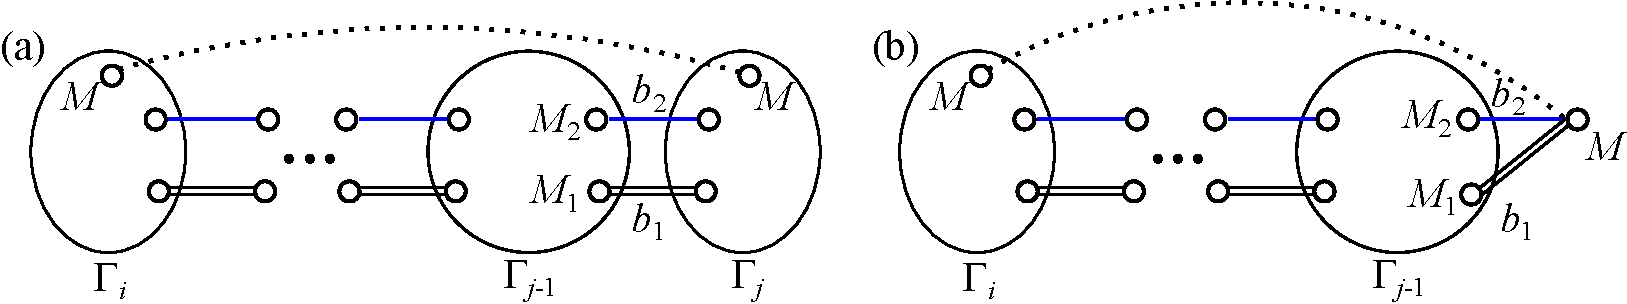
\includegraphics[width=13cm]{graph_adddot1.pdf}}
\end{equation}
Here we keep the names $\Gamma_l$, $i \le l \le j$, for the subgraph components inside the black circles. We also keep the dotted edge between $\Gamma_i$ and $\Gamma_j$ in order to have a clearer comparison with the original graph without this dotted edge. In particular, the ending molecules of this dotted edge should be understood as the same molecule, denoted by $\cal M$.

	
First, by the SPD property of the original graph $\cal G$, we know that the component $\Gamma_j$ in graph (a) of \eqref{graph_adddot1} is pre-deterministic, and hence we can change the blue solid edges in it into $\dashed$ edges one by one according to a pre-deterministic order. 
%\iffalse
%Then we get the first graph of \eqref{graph_adddot1}, where $\Gamma_j$ contains no plus $G$ edges and is doubly connected: 
%	\begin{equation}%\label{graph_adddot1}
%		\parbox[c]{0.9\linewidth}{\center
%			\includegraphics[width=14cm]{graph_adddot1.png}}
%	\end{equation}
%	Here as in \eqref{eq_keepdot}, we keep the dotted edge between two molecules in $\Gamma_i$ and $\Gamma_j$ in order to have a clearer comparison with the original graph without the dotted edge. 
%\fi
By Claim \ref{trivial_graph1}, graph (a) of \eqref{graph_adddot1} is equivalent (in the sense of doubly connected property) to graph (b) of \eqref{graph_adddot1} with $\Gamma_j$ replaced by a vertex. Furthermore, by merging the molecules connected by the dotted edge, we get the following graph (a): % of \eqref{graph_adddot1}. 
	\begin{equation}\label{graph_adddot2}
	\parbox[c]{0.8\linewidth}{\center
		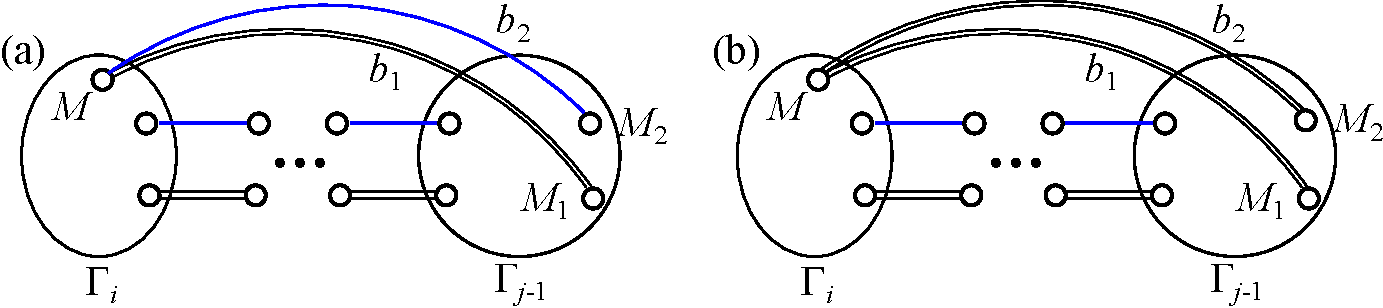
\includegraphics[width=11cm]{graph_adddot2.pdf}}
\end{equation}
%Hence, it suffices to show that the graph (a) in \eqref{graph_adddot2} is pre-deterministic. 
We claim that $b_2$ is redundant in graph (a) of \eqref{graph_adddot1}. Due to the doubly connected property of the original graph $\cal G$ and the above fact, removing the subgraph $\Iso_{j}$ and its two external edges still gives a doubly connected graph. Correspondingly, in graph (a) of \eqref{graph_adddot2}, if we remove the edges $b_1$ and $b_2$, we still get a doubly connected graph, so the edge $b_2$ is redundant. Then we can change $b_2$ into a $\dashed$ edge and get graph (b) of \eqref{graph_adddot2}.
	
%By property (i) of Definition \ref{def seqPDG}, we can check that removing the component $\Gamma_j$ and its external dotted, blue solid and $\dashed$ edges in the first graph of \eqref{graph_adddot1} leads to a graph that is doubly connected. (Otherwise, the original graph $\cal G$ cannot be doubly connected due to the fact that $\Iso_j$ is isolated in $\cal G$.)   Then the second graph in \eqref{graph_adddot1} is obtained by adding two extra edges $b_1$ and $b_2$ to a doubly connected graph. Hence $b_2$ is redundant, and we can change it into a $\dashed$ edge as in the following graph
%	\begin{equation}%\label{graph_adddot2}
%		\parbox[c]{0.8\linewidth}{\center
%			\includegraphics[width=4cm]{graph_adddot2.png}}
%	\end{equation}
	
Next, by property (iii) of Definition \ref{def seqPDG}, if we replace $b_1$ and $b_2$ with a single $\dashed$ edge $b$ between $\cal M_1$ and $\cal M_2$ in graph (b) of \eqref{graph_adddot2}, the component $\Gamma_{j-1}$ in the resulting graph becomes pre-deterministic.  
%component $\Gamma_j$ and its external dotted, blue solid and $\dashed$ edges with a $\dashed$ edge $b$ between $\cal M_1$ and $\cal M_2$ in the first graph of \eqref{graph_adddot1}, then the component $\Gamma_{j-1}$ in the resulting graph, say $\cal G'$, becomes pre-deterministic. Note that the graph \eqref{graph_adddot2} is obtained by replacing the $\dashed$ edge $b$ in $\cal G'$ with a path of two black $\dashed$ edges from $\cal M_1$ to $\cal M$, and from $\cal M$ to $\cal M_{2}$. 
Then using Claim \ref{trivial_graph3}, we get that the component $\Gamma_{j-1}$ in graph (b) of \eqref{graph_adddot2} is pre-deterministic, and we can change the blue solid edges in it into $\dashed$ edges one by one. % according to the same pre-deterministic order as in the component $\Gamma_{j-1}$ of graph $\cal G'$. 
After that, the subgraph induced on the molecule $\cal M$ and the molecules in $\Gamma_{j-1}$ is a doubly connected graph. Indeed, by the above fact, the subgraph induced on the molecules in $\Gamma_{j-1}$ is doubly connected (also after its blue solid edges are changed into $\dashed$ edges), and $\cal M$ is connected to it through the two $\dashed$ edges $b_1$ and $b_2$, which we add to the black net and the blue net, respectively. (Note that this uses the doubly connected property of the subgraph induced on $\Gamma_{j-1}$ itself, and not only that of $\Gamma_{j-1}$ together with the $\dashed$ edge $b$ between $\cal M_1$ and $\cal M_2$: a doubly connected graph does not remain doubly connected in general if one of its edges is replaced with a path of two edges through a new molecule.) Thus we can replace this subgraph with a vertex by Claim \ref{trivial_graph1} and obtain a graph with a similar structure as graph (a) of \eqref{graph_adddot2}.
%\begin{center}
%\includegraphics[width=4.5cm]{graph_adddot3.png}
%\end{center}
%Notice that it has a similar structure as the third graph in \eqref{graph_adddot1}. 
Hence we can repeat exactly the same argument again. 
	
Continuing in this way, we can show that the blue solid edges in $\Iso_{i}$ can be changed into $\dashed$ edges one by one according to an order given by the above argument. Hence $\Iso_{i}$ is pre-deterministic. 
\end{proof}

%\iffalse
%Now we claim that the edge $(x,\al)$ is redundant. To prove this fact, we put $(y,\beta)$ into the black net and the dotted edge $(w,\gamma)$ into the blue net. By the definition of SPD graph, if we remove the dotted edge $(w,\gamma)$ and replace $\overline I_j$ with a blue edge $(x,y)$, then the edge $(x,y)$ is a redundant edge in $I_i^{(1)}$. This means that there exist both a connected black net and a connected blue net inside the component $I_i^{(1)}$ without using the edge $(x,y)$. 
%Thus in the above graph, the $\dashed$ edge $(y,\beta)$ connects the black nets in $I_i^{(1)}$ and $I_j$
%and gives a connected black net of $I_i$. Moreover, there exists a blue path from $x$ to $\al$ without going through the edge $(x,\al)$ as follows: we can go from $x$ to $w$ through a blue path inside $I_i^{(1)}$, then from $w$ to $\gamma$ through the dotted edge $(w,\gamma)$, and finally from $\gamma$ to $\al$ through a blue path inside $I_j$. Thus without the edge $(x,\al)$, $I_i$ is still doubly connected, which shows that $(x,\al)$ is redundant. 
%
%Now we change $(x,\al)$ into a $\dashed$ edge and get the following graph.
%\begin{equation}\label{graphadddot2}
%	\parbox[c]{0.8\linewidth}{\center
%		\includegraphics[width=7cm]{adddot2.png}}
%\end{equation}
%Recall that if we remove the dotted edge $(w,\gamma)$ and replace the component $\overline I_j$ with a blue edge $b_1=(x,y)$, then the isolated subgraph $I_{j-1}$ becomes pre-deterministic. In other words, there exists a pre-deterministic order of all the plus $G$ edges in $\Gamma_{j-1}$, say $b_1,b_2,\cdots$. We now show that in graph \eqref{graphadddot2}, the edges $b_2, b_3, \cdots, $
%can be changed into $\dashed$ edges one by one according to this order. For the edge $b_2$, we know that if $b_1$ becomes a $\dashed$ edge between $x$ and $y$, then $b_2$ is redundant. There are two cases: (a) the $\dashed$ edge $b_1$ is included in the blue net in order for $b_2$ to be redundant, and (b) the $\dashed$ edge $b_1$ is included in the black net in order for $b_2$ to be redundant. 
%\begin{itemize}
%	\item 
%	For case (a), as in \eqref{graphadddot2} we include the dotted edge $(w,\gamma)$ into the black net, while include edges $(x,\al)$, $(y,\beta)$ into the blue net. Then the edge $(w,\gamma)$ connects the black nets of $I_{i}^{(1)}$ and $I_{j}$ to give a connected black net of $I_i$. On the other hand, $x$ and $y$ are connected with a path of blue edges through the edge $(x,\al)$, a blue path from $\al$ to $\beta$ in $I_{j}$, and the edge $(\beta,y)$. This path plays the same role as a single $\dashed$ edge $b_1$ between $x$ and $y$, and hence $b_2$ is redundant. 
%	\item For case (b), we put the dotted edge $(w,\gamma)$ into the blue net and edges $(x,\al)$ and $(y,\beta)$ into the black net. Then a similar argument as above shows that $b_2$ is redundant.
%\end{itemize}
%After turning $b_2$ into a $\dashed$ edge, with similar argument as above we can show that $b_3$ is redundant. Continuing the argument in this way, we can show that the edges $b_2, b_3, \cdots, $ in $\Gamma_{j-1}$ can be changed into $\dashed$ edges one by one according to this order.
%
%After turning all plus $G$ edges in $I_{j-1}$ into $\dashed$ edges, we get a graph that looks like \eqref{graphadddot3}. We now claim the the blue edge $(x_1,x_2)$ connecting $I_{j-1}$ to the component $\Gamma_{j-2}$ (which is a subgraph of $I_i^{(2)}$) is redundant. The proof is similar to the above argument for the edge $(x,\al)$. First notice that the components $I_{i}^{(2)}$, $\Gamma_{j-1}$ and $I_j$ are all doubly connected by the definition of SPD graph. Then we put the edges $(y_1,y_2)$ and $(x,\al)$ into black net, and they connects the black nets in $I_{i}^{(2)}$, $\Gamma_{j-1}$ and $I_j$ to give a connected black net of $I_i$. On the other hand, we put edges $(y,\beta)$ and $(w,\gamma)$ into blue net. Then $x_1$ and $x_2$ are connected through a blue path without using the edge $(x_1,x_2)$: we can go from $x_2$ to $w$ through a blue path inside $I_i^{(2)}$, from $w$ to $\gamma$ through the dotted edge $(w,\gamma)$, from $\gamma$ to $\beta$ through a blue path  inside $I_j$, from $\beta$ to $y$ through the edge $(y,\beta)$, and finally from $y$ to $x_1$ through a blue path inside $\Gamma_{j-1} $. Hence the blue edge $(x_1,x_2)$ is redundant.
%%(here $I_{j-1}$ is doubly connected because by replacing $\overline I_j$ with a blue edge, this edge is redundant in $I_{j-1}$). 
%\begin{equation}\label{graphadddot3}
%	\parbox[c]{0.8\linewidth}{\center
%		\includegraphics[width=8cm]{adddot3.png}}
%\end{equation}
%%have the above graph, where we put dotted edge $(y,\gamma)$ into the blue net and edges $(x,\al)$ and $(y,\beta)$ into the black net. Then the edge $(y,\gamma)$ connects the blue nets of $I_{k}^{(1)}$ and $I_{k}^{(2)}$. On the other hand, $x$ and $y_1$ are connected with a path of black edges through the edge $(x,\al)$, a black path from $\al$ to $\beta$ in $I_{k}^{(2)}$, and the edge $(\beta,y)$. This path plays the same role as the $\dashed$ edge $d_1$, and hence $b_2$ is redundant.
%%\begin{center}
%%\includegraphics[width=7cm]{Recolli4.png}
%%\end{center}
%
%
%By the sequential pre-deterministic property, if we remove the dotted edge $(w,\gamma)$ and replace the component $\overline I_{j-1}$ with a blue edge $\wt b_1=(x_2,y_2)$, then the isolated subgraph $I_{j-2}$ becomes a pre-deterministic graph. In other words, there exists a pre-deterministic order of $\wt b_1$ and all the plus $G$ edges in $\Gamma_{j-2}$, denoted by $\wt b_1,\wt b_2,\cdots$. We can show that the edges $\wt b_2,\wt b_3, \cdots, $ can be changed into $\dashed$ edges one by one according to this order. The proof is the same as the one for the blue edges $b_2,b_3,\cdots$ in $\Gamma_{j-1}$, so we omit the details. 
%
%Continuing the above argument, we can turn the blue edges in $I_i$ into $\dashed$ edges one by one, such that at each step the corresponding blue edge is redundant. This concludes the first statement of Lemma \ref{hard lemmdot}.
%
%For the second statement, the above arguments for the first statement shows that the maximal isolated subgraph $I_0$ becomes redundant after replacing $\overline I_{j+1}$ with a blue edge. Then we change the plus $G$ edges in $I_0$ into $\dashed$ edges one by one, and it remains to show that the solid blue edge connected with $\oplus$ is redundant. Suppose the dotted edge is connected to $\oplus$. Then we have the following graph:
%\begin{equation*} 
%	\parbox[c]{0.8\linewidth}{\center
%		\includegraphics[width=7cm]{adddot4.png}}
%\end{equation*}
%If we put the dotted edge $(\gamma,\oplus)$ into the blue net and $(y,\otimes)$ into the black net, then $x$ is connected to $\oplus$ through a blue path without using the edge $(x,\oplus)$: we can go from $x$ to $\gamma$ through a blue path inside $I_0$, and then from $\gamma$ to $\oplus$ through the edge $(\gamma,\oplus)$. Thus $(x,\otimes)$ is redundant in the sense of Definition \ref{def 2netex}, and the whole graph is a pre-deterministic graph. 
%%(As another choice, we can also put the dotted edge $(\gamma,\oplus)$ into the black net and $(y,\otimes)$ into the blue net, then $x$ and all the internal molecules are connected to $\otimes$ through a blue net, and to $\oplus$ through a black net. The edge $(x,\otimes)$ is still redundant.) 
%If the dotted edge is connected to $\otimes$ or $\ominus$, the argument is similar. Hence we conclude the second statement.  
%\fi

%The proof of Lemma \ref{hard lemmQ} is similar to the above proof for Lemma \ref{hard lemmdot} in certain sense, but there are many more cases to consider. 

The proof of the case (i) of Lemma \ref{hard lemmQ} uses Claim \ref{trivial_graph1} and the following three claims.   

\begin{claim}\label{trivial_graph4}
Given a doubly connected graph $\cal G$, we construct a new graph $\cal G_{new}$ as follows: we create a new molecule $\cal M_{new}$; we add a $\dashed$ edge $b_1$ between $\cal M_{new}$ and a molecule $\cal M_1$ in $\cal G$, and a blue solid edge $b_2$ between $\cal M_{new}$ and a molecule $\cal M_2$ in $\cal G$; we replace a blue solid edge $b$ between molecules $\cal M_3$ and $\cal M_4$ in $\cal G$ with two blue solid edges $b_3$ between $\cal M_3$ and $\cal M_{new}$ and $b_4$ between $\cal M_4$ and $\cal M_{new}$. Then the blue solid edge $b_2$ is redundant in $\cal G_{new}$.
\end{claim}
\begin{proof}
We illustrate the setting of this claim with the following figure, where graphs (a) and (b) represent $\cal G$ and $\cal G_{new}$, respectively:
\begin{equation} \label{eq_add_Q1}
\parbox[c]{0.5\linewidth}{\center 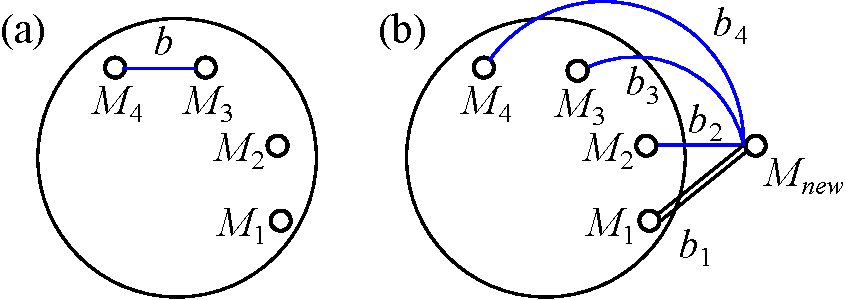
\includegraphics[width=7cm]{add_Q1.pdf}} 
\end{equation}
The original graph $\cal G$ is doubly connected with black and blue nets denoted by $\cal B_{black}$ and $\cal B_{blue}$. In $\cal G_{new}$, the edge $b_1$ connects the new molecule $\cal M_{new}$ to $\cal M_1$, and hence $\cal B_{black} \cup\{b_1\}$ is a black net in $\cal G_{new}$. Moreover, the path of edges $b_3$ and $b_4$ in $\cal G_{new}$ can replace the role of $b$ in the blue net $\cal B_{blue}$, and they also connect $\cal M_{new}$ to the molecules in $\cal G$. Hence $\cal B_{blue} \cup\{b_3,b_4\}\setminus \{b\}$ is a blue net in $\cal G_{new}$. Since $b_2$ is not used in this blue net, it is redundant in $\cal G_{new}$.
\end{proof}
	
	
\begin{claim}\label{trivial_graph5}
Given a doubly connected graph $\cal G$, we construct a new graph $\cal G_{new}$ as follows: we create a new molecule $\cal M_{new}$; we replace a $\dashed$ edge $b_0$ between molecules $\cal M_1$ and $\cal M_2$ in $\cal G$ with two $\dashed$ edges $b_1$ between $\cal M_1$ and $\cal M_{new}$, and $b_2$ between $\cal M_2$ and $\cal M_{new}$; we replace a blue solid edge $b$ between molecules $\cal M_3$ and $\cal M_4$ in $\cal G$ with two blue solid edges $b_3$ between $\cal M_3$ and $\cal M_{new}$, and $b_4$ between $\cal M_4$ and $\cal M_{new}$. Then we have that:
\begin{itemize}
\item[(i)] If a blue solid edge is not equal to $b$ and is redundant in $\cal G$, then it is also redundant in $\cal G_{new}$. 
			
\item[(ii)] If the edge $b$ is redundant in $\cal G$, then either $b_3$ or $b_4$ is redundant. Moreover, if we change one redundant edge of them into a $\dashed$ edge, the other edge also becomes redundant. 
\end{itemize}
\end{claim}
\begin{proof}
%In the proof of this claim, we will use the following simple fact: a blue edge $e=(\cal M, \cal M')$ is redundant in the blue net if and only if there exists another molecule $\cal M''$ and two connected paths of blue edges, such that one of them connects $\cal M$ to $\cal M''$, another one connects $\cal M'$ to $\cal M''$, and both of these two paths do not contain the edge $e$. %through which we can go from $x$ to $y$ without using the edge $(x,y)$.
We first prove the statement (i). Suppose the redundant blue solid edge we are considering is $e=(\cM_5,\cM_6)$. We consider two cases: (A) the edge $b_0$ is included in the black net of $\cal G$ in order for $e$ to be redundant, and (B) the edge $b_0$ is included in the blue net of $\cal G$ in order for $e$ to be redundant. 
		
\vspace{5pt}
\noindent {\bf Case (A):} The graphs (a) and (b) of the following figure represent $\cal G$ and $\cal G_{new}$, respectively: 
%where we only draw the isolated subgraph $I_i$. The right graph gives the subgraph $I_i$ we are considering, and the left graph gives the subgraph $I_i$ obtained by replacing the path $a\to \gamma\to b$ with a blue edge $(a,b)$ and the component $\overline I_j$ with a $\dashed$ edge $b_1=(x,y)$. 
\begin{equation} \label{eq_add_Q2}
\parbox[c]{0.8\linewidth}{\center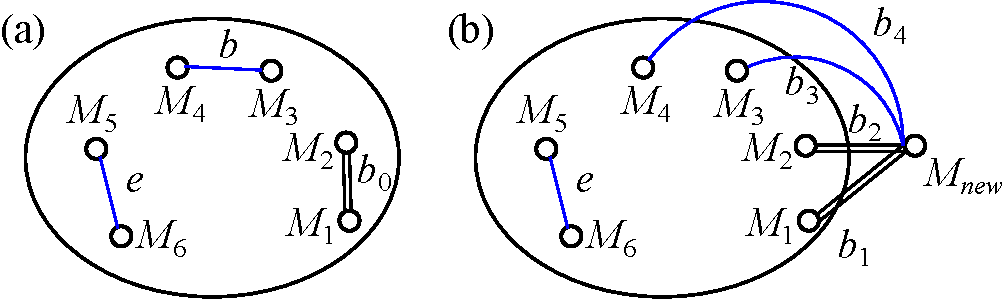
\includegraphics[width=8.5cm]{add_Q2.pdf}}
\end{equation}
In graph $\cal G$, the edge $e=(\cM_5,\cM_6)$ is redundant by putting $b_0$ into the black net. Let the corresponding black net and blue net be $\cal B_{black}$ and $\cal B_{blue}$, such that $b_0\in \cal B_{black}$ and $\cal B_{blue} \setminus \{e\}$ is still a blue net of $\cal G$. Then in $\cal G_{new}$, if we put edges $b_1$ and $b_2$ into the black net, they can replace the role of $b_0$ in the black net $\cal B_{black}$ and also connect $\cal M_{new}$ to other molecules. Hence $\cal B_{black} \cup\{b_1,b_2\}\setminus \{b_0\}$ is a black net in $\cal G_{new}$. Similarly, the path of edges $b_3$ and $b_4$ can replace the role of $b$ in the blue net $\cal B_{blue} \setminus \{e\}$ and also connect $\cal M_{new}$ to other molecules. Hence $\cal B_{blue} \cup\{b_3,b_4\}\setminus \{e, b\}$ is a blue net in $\cal G_{new}$. Since $e$ is not used in this blue net, it is redundant in $\cal G_{new}$.
		
		
\vspace{5pt}
\noindent {\bf Case (B):} The graphs (a) and (b) of the following figure represent $\cal G$ and $\cal G_{new}$, respectively:  
\begin{equation} \label{eq_add_Q3}
\parbox[c]{0.8\linewidth}{\center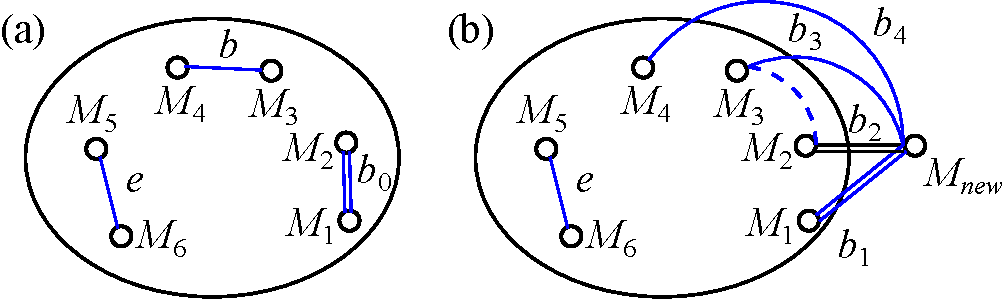
\includegraphics[width=8.5cm]{add_Q3.pdf}}
\end{equation}
In graph $\cal G$, the edge $e=(\cM_5,\cM_6)$ is redundant by putting $b_0$ into the blue net.  Let the corresponding black net and blue net be $\cal B_{black}$ and $\cal B_{blue}$, such that $b_0\in \cal B_{blue}$ and $\cal B_{blue}\setminus \{e\}$ is still a blue net of $\cal G$. Then either $\cal M_1$ or $\cal M_2$ is connected to molecules $\cal M_3$ and $\cal M_4$ through a path of edges in $\cal B_{blue}\setminus \{e,b_0\}$, since otherwise adding back the edge $b_0$ to $\cal B_{blue}\setminus \{e,b_0\}$ does not give a blue net, which is a contradiction. Without loss of generality, assume that $\cal M_2$ is connected to $\cal M_3$ through a path of edges in $\cal B_{blue}\setminus \{e,b_0,b\}$. In graph (b) of \eqref{eq_add_Q3}, the dashed edge represents such a path from $\cal M_2$ to $\cal M_3$.
 
%at least one of the molecules $x_2$ and $y_2$ must be connected to $a$ and $b$ through a blue path without using $b_1=(x,y)$ and $b_2=(x_2,y_2)$. Without loss of generality, assume that this molecule is $y_2$. 
%By a similar argument, $\cal M_3$ and $\cal M_4$ must be connected with either $\cal M_1$ or $\cal M_2$ through a path of edges in $\cal B_2\setminus \{e,b_0\}$. Without loss of generality, assume that $\cal M_3$ and $\cal M_4$ are connected with $\cal M_2$ through a path of edges in $\cal B_2\setminus \{e,b_0\}$. 
%We draw one possible scenario in the second graph of \eqref{eq_add_Q3}. 
%Without loss of generality, assume that $x_2$ is connected with $x$ through a blue path without using $b_1$ and $b_2$. Then as in the right graph, 
		
Now in graph (b) of \eqref{eq_add_Q3}, we put $b_1$ into the blue net and $b_2$ into the black net. Then  $\cal B_{black}\cup\{b_2\}$ is a black net in $\cal G_{new}$, because $b_2$ connects the new molecule $\cal M_{new}$ to other molecules. On the other hand, we claim that $\cal B^{new}_{blue}:=\cal B_{blue}\cup \{b_1, b_3,b_4\}\setminus \{e,b_0,b\}$ is a blue net in $\cal G_{new}$. This can be derived from the following observations.
\begin{itemize}
\item[(1)] $\cM_3$ and $\cM_4$ are connected by the path of edges $b_3$ and $b_4$, which replaces the role of edge $b$ in the blue net $\cal B_{blue} \setminus \{e\}$ of $\cal G$.

\item[(2)] $\cM_1$ and $\cM_2$ is connected by a path of edges in $\cal B^{new}_{blue}$ consisting of $b_1$, $b_3$ and a path of edges connecting $\cal M_2$ to $\cal M_3$ in $\cal B_{blue}\setminus \{e,b_0, b\}$. This shows that the role of edge $b_0$ in the blue net $\cal B_{blue} \setminus \{e\}$ can be replaced by a path of edges in $\cal B^{new}_{blue}$.
			
\item[(3)] The new molecule $\cal M_{new}$ is connected to other molecules through $b_1$, $b_3$ and $b_4$.
\end{itemize}
Combing these observations with the fact that $\cal B_{blue}\setminus \{e\}$ is a blue net in $\cal G$, we conclude that $\cal B^{new}_{blue}$ is a blue net in $\cal G_{new}$. Since $e$ is not in this blue net, it is redundant in $\cal G_{new}$.
		
\medskip
		
Next we prove the statement (ii). Again there are two cases: (C) the edge $b_0$ is included in the black net of $\cal G$ in order for $b$ to be redundant, and (D) the edge $b_0$ is included in the blue net of $\cal G$ in order for $b$ to be redundant. 

 
		
\vspace{5pt}
\noindent {\bf Case (C):} In this case, $\cal G$ and $\cal G_{new}$ are represented by the graphs (a) and (b) of \eqref{eq_add_Q2} (where the edge $e$ is irrelevant). The graph $\cal G$ has a black net $\cal B_{black}$ and a blue net $\cal B_{blue}$, such that $b_0\in \cal B_{black}$ and $\cal B_{blue} \setminus \{b\}$ is still a blue net of $\cal G$. Then in $\cal G_{new}$, 
%if we put edges $b_1$ and $b_2$ into the black net, they can replace the role of $b_0$ in the black net $\cal B_{black}$ and also connect $\cal M_{new}$ to other molecules. Hence 
we again have that $\cal B_{black} \cup\{b_1,b_2\}\setminus \{b_0\}$ is a black set in $\cal G_{new}$. On the other hand, $\cal B_{blue} \cup \{b_4\}\setminus \{b\}$ is a blue net in $\cal G_{new}$, because $\cal B_{blue} \setminus \{b\}$ is a blue net in $\cal G$ and $b_4$ connects $\cal M_{new}$ to other  molecules.  Since $b_3$ is not used in this blue net, it is redundant in $\cal G_{new}$. Hence we can change $b_3$ into a $\dashed$ edge. With the same argument, we can show that $b_4$ is also redundant in the new graph. This concludes statement (ii) for case (C).

%and get the following graph, where, for simplicity, we still denote it by $\cal G_{new}$:
%\begin{equation} \label{eq_add_Q4}
%\parbox[c]{0.8\linewidth}{\center\includegraphics[width=12cm]{add_Q4.png}}
%\end{equation}
%We again put edges $b_1$ and $b_2$ into the black net, and put edge $b_3$ into the blue net. Then with a similar argument as above, we can check that $\cal B_1 \cup\{b_1,b_2\}\setminus \{b_0\}$ is a black set in $\cal G_{new}$, and $\cal B_2 \cup \{b_3\}\setminus \{b\}$ is a blue net in $\cal G_{new}$. Since $b_4$ is not  in this blue net, it is redundant in $\cal G_{new}$.

		
\vspace{5pt}
\noindent {\bf Case (D):} In this case, $\cal G$ and $\cal G_{new}$ are represented by the graphs (a) and (b) of \eqref{eq_add_Q3} (where the edge $e$ is irrelevant). The graph $\cal G$ has a black net $\cal B_{black}$ and a blue net $\cal B_{blue}$, such that $b_0\in \cal B_{blue}$ and $\cal B_{blue} \setminus \{b\}$ is still a blue net in $\cal G$. By a similar argument as in case (B), either $\cal M_3$ or $\cal M_4$ is connected to one of $\cal M_1$ and $\cal M_2$ through a path of edges in $\cal B_{blue}\setminus \{b,b_0\}$. 
%Then either $\cal M_3$ or $\cal M_4$ is connected to one of the molecules $\cal M_1$ and $\cal M_2$ through a path of edges in $\cal B_2\setminus \{b,b_0\}$ (otherwise, after adding back edge $b_0$ to $\cal B_2\setminus \{e,b_0\}$ does not give a blue net $\cal B_2\setminus \{b\}$, which gives a contradiction). 
Without loss of generality, assume that $\cal M_3$ is connected to $\cal M_2$ through a path of edges in $\cal B_{blue}\setminus \{b,b_0\}$ (which is represented by the dashed edge in graph (b) of \eqref{eq_add_Q3}). %The second graph of \eqref{eq_add_Q3} shows one such scenario. 
First, we again have that $\cal B_{black}\cup\{b_2\}$ is a black net in $\cal G_{new}$. Then we claim that $\cal B^{new}_{blue}:=\cal B_{blue}\cup \{b_1, b_3\}\setminus \{b,b_0\}$ is a blue net in $\cal G_{new}$. This claim follows from the observation that $\cM_1$ and $\cM_2$ are connected by a path of edges in $\cal B^{new}_{blue}$ consisting of $b_1$, $b_3$ and a path of edges connecting $\cal M_2$ to $\cal M_3$ in $\cal B_{blue}\setminus \{b,b_0\}$, and hence the role of edge $b_0$ in $\cal B_{blue}\setminus \{b\}$ can be replaced by a path of edges in $\cal B^{new}_{blue}$. Since $b_4$ is not used in $\cal B^{new}_{blue}$, it is redundant in $\cal G_{new}$.
		
Now we change $b_4$ into a $\dashed$ edge and get the following graph, denoted by $\wt{\cal G}_{new}$: %, where, for simplicity, we still denote it by $\cal G_{new}$:
\begin{equation} \label{eq_add_Q5}
\parbox[c]{0.8\linewidth}{\center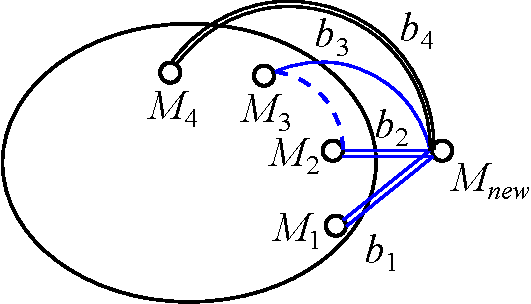
\includegraphics[width=4.7cm]{add_Q5.pdf}}
\end{equation}
We put $b_4$ into the black net, and $b_1$ and $b_2$ into the blue net. Then it is easy to see that $\cal B_{black}\cup\{b_4\}$ is a black net in $\cal G_{new}$. Moreover, $\cal B_{blue}\cup \{b_1, b_2\} \setminus \{b,b_0\}$ is a blue net in $\cal G_{new}$, because the path of edges $b_1$ and $b_2$ can replace the role of edge $b_0$ in the original blue net $\cal B_{blue}\setminus \{b\}$ of $\cal G$, and $b_1$ and $b_2$ also connect $\cal M_{new}$ to other molecules. Since $b_3$ is not used in this blue net, it is redundant in $\cal G_{new}$. This concludes the statement (ii) for case (D).
\end{proof}
	
\begin{claim}\label{trivial_graph6}
Given a doubly connected graph $\cal G$, we construct a new graph $\cal G_{new}$ as follows: we create a new molecule $\cal M_{new}$; we replace a $\dashed$ edge $b_0$ between molecules $\cal M_1$ and $\cal M_2$ in $\cal G$ with two $\dashed$ edges $b_1$ between $\cal M_1$ and $\cal M_{new}$, and $b_2$ between $\cal M_2$ and $\cal M_{new}$; we replace a $\dashed$ edge $b$ between molecules $\cal M_3$ and $\cal M_4$ in $\cal G$ with two $\dashed$ edges $b_3$ between $\cal M_3$ and $\cal M_{new}$, and $b_4$ between $\cal M_4$ and $\cal M_{new}$. If a blue solid edge is redundant in $\cal G$, then it is also redundant in $\cal G_{new}$.
\end{claim}
\begin{proof}
Suppose the redundant blue solid edge we are considering is $e=(\cM_5,\cM_6)$. If the edge $b$ is included into the blue net in order for $e$ to be redundant in $\cal G$, we put the edges $b_3$ and $b_4$ into the blue net, and the result then follows from Claim \ref{trivial_graph5} (because blue $\dashed$ edges and blue solid edges are equivalent in a blue net). Notice that $b_0$ and $b$ play symmetric roles. Hence if $b_0$ is included into the blue net in order for $e$ to be redundant in $\cal G$, we can conclude the proof with the same argument. 

It remains to consider the case where both $b$ and $b_0$ are included into the black net in order for $e$ to be redundant in $\cal G$. We have the following figure, where the graphs (a) and (b) respectively represent $\cal G$ and $\cal G_{new}$:
\begin{equation} \label{eq_add_Q6}
\parbox[c]{0.8\linewidth}{\center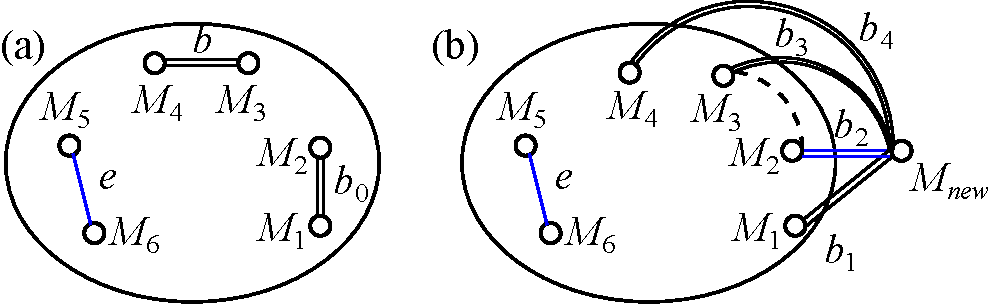
\includegraphics[width=8.5cm]{add_Q6.pdf}}
\end{equation}
The graph $\cal G$ has a black net $\cal B_{black}$ and a blue net $\cal B_{blue}$, such that $b_0, b\in \cal B_{black}$ and $\cal B_{blue} \setminus \{e\}$ is still a blue net of $\cal G$. Then either $\cal M_3$ or $\cal M_4$ is connected to one of $\cal M_1$ and $\cal M_2$ through a path of black edges in $\cal B_{black}\setminus \{b,b_0\}$, since otherwise adding back the edges $b$ and $b_0$ to $\cal B_{black}\setminus \{b,b_0\}$ does not give a black net, which is a contradiction. Without loss of generality, assume that $\cal M_3$ is connected to $\cal M_2$ through a path of edges in $\cal B_{black}\setminus \{b,b_0\}$, which is represented by the dashed edge in the graph (b) of \eqref{eq_add_Q6}. %The second graph of \eqref{eq_add_Q6} shows one such scenario. 
Then in $\cal G_{new}$, we put $b_2$ into the blue net, and put edges $b_1$, $b_3$ and $b_4$ into the black net. First, using the fact that $\cal B_{blue} \setminus \{e\}$ is a blue net in $\cal G$, it is easy to see that $\cal B_{blue} \cup\{b_2\}\setminus \{e\}$ is a blue net in $\cal G_{new}$. Then we claim that $\cal B^{new}_{black}:=\cal B_{black}\cup \{b_1, b_3,b_4\}\setminus \{b,b_0\}$ is a black net in $\cal G_{new}$. This is due to the following observations.
\begin{itemize}
\item[(1)] $\cM_3$ and $\cM_4$ are connected by the path of edges $b_3$ and $b_4$, which replaces the role of edge $b$ in the original black net $\cal B_{black}$.
			
\item[(2)] $\cM_1$ and $\cM_2$ are connected by a path of edges in $\cal B^{new}_{black}$ consisting of $b_1$, $b_3$ and a path of black edges connecting $\cal M_2$ to $\cal M_3$ in $\cal B_{black}\setminus \{b,b_0\}$. This shows that the role of edge $b_0$ in the original black net $\cal B_{black}$ can be replaced by a path of edges in $\cal B^{new}_{black}$.
			
\item[(3)] The new molecule $\cal M_{new}$ is connected to other molecules through $b_1$, $b_3$ and $b_4$.
\end{itemize}
Hence $\cal G_{new}$ has a black net $\cal B^{new}_{black}$ and a blue net $\cal B_{blue}\cup\{b_2\} \setminus \{e\}$. Since $e$ is not used in this blue net, it is redundant.
\end{proof}
	
Now we give the proof of the case (i) of Lemma \ref{hard lemmQ} using Claims \ref{trivial_graph4}--\ref{trivial_graph6}. Recall that the original graph is denoted by $\cal G$, and the new graph is denoted by $\wt{\cal G}$. In Lemma \ref{hard lemmQ}, the case $\cal M=\cal M'$ can only occur in the cases (i) and (ii). In this case, the replaced blue solid edge $b$ between $\cal M$ and $\cal M'$ lies inside the molecule $\cal M$, so it does not appear in the molecular graph, and the two new blue solid edges $b_3$ and $b_4$ both connect $\cal M$ and $\cal M''$. The proofs below hold without change: Claims \ref{trivial_graph4}--\ref{trivial_graph6} and their proofs hold verbatim when $\cal M_3=\cal M_4$, with the edge $b$ removed from all nets (it is not needed to connect $\cal M_3$ and $\cal M_4$), and a blue solid edge inside a molecule is redundant, so it can be placed anywhere in a pre-deterministic order.
\begin{proof}[Proof of Lemma \ref{hard lemmQ}: case (i)]
%For simplicity of presentation, in the following proof, we only focus on the isolated subgraphs $\Iso_i$. Moreover, whenever we say that ``we can change a blue solid edge into a $\dashed$ edge", we actually mean that ``we know that this edge is redundant and we then change it into a $\dashed$ edge". 
The statement that $\Iso_{j+1}$ is the maximal isolated subgraph of $\Iso_i$ is trivial. We replace $\Iso_{j+1}$ and its two external edges with a $\dashed$ edge, and get the following graph (a) for the isolated subgraph $\Iso_i$ of $\wt{\cal G}$:
\begin{equation} \label{graph_add_Q7}
\parbox[c]{0.9\linewidth}{\center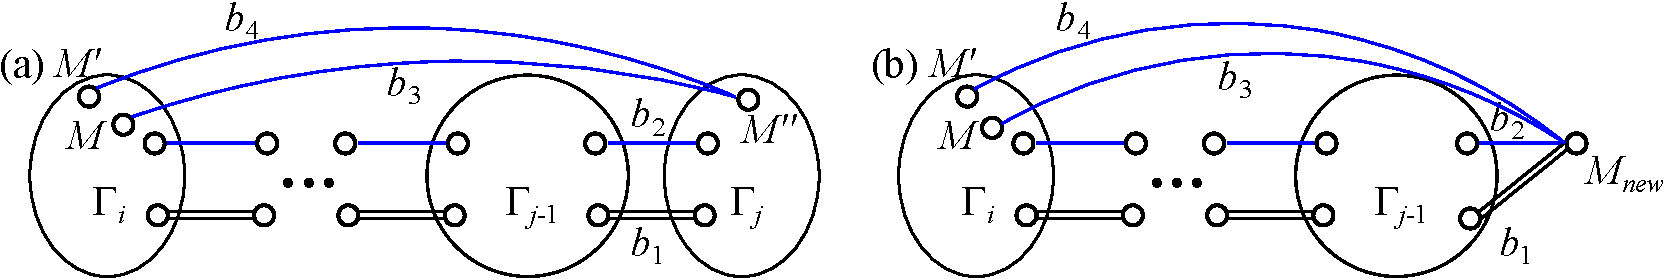
\includegraphics[width=14cm]{add_Q7.pdf}}
\end{equation}
Here we keep the names $\Gamma_l$, $i \le l \le j$, for the subgraph components inside the black circles. By the SPD property of $\cal G$, we know that the component $\Gamma_j$ in graph (a) is pre-deterministic, and hence we can change its blue solid edges into $\dashed$ edges one by one according to a pre-deterministic order. 
% Then we get the first graph of \eqref{graph_add_Q7}, where $\Gamma_j$ contains no plus $G$ edges and is doubly connected: 
%		\begin{equation}% \label{graph_add_Q7}
%			\parbox[c]{0.9\linewidth}{\center
%				\includegraphics[width=15cm]{add_Q7.png}}
%		\end{equation}
Now by Claim \ref{trivial_graph1}, %to show graph (a) of \eqref{graph_add_Q7} is pre-deterministic, 
it suffices to show that the graph (b) with $\Gamma_j$ replaced by a vertex is pre-deterministic. 

Now we show that the edge $b_2$ is redundant in the graph (b) of \eqref{graph_add_Q7}. By the doubly connected property of $\cal G$, removing the subgraph $\Iso_{j+1}$ and its two external edges still gives a doubly connected graph. Correspondingly, in the graph (b) of \eqref{graph_add_Q7}, if we remove the two edges $b_1$ and $b_2$ and replace the edges $b_3$ and $b_4$ with a single blue solid edge $b=(\cal M, \cal M')$, we still get a doubly connected graph. Then by Claim \ref{trivial_graph4}, the edge $b_2$ is redundant, so we can change it into a $\dashed$ edge and get the following graph: % and get the third graph of \eqref{graph_add_Q7}.
\begin{equation} \label{graph_add_Q75}
\parbox[c]{0.4\linewidth}{\center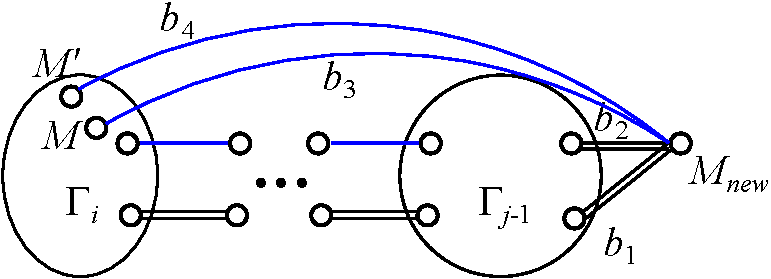
\includegraphics[width=6.5cm]{add_Q75.pdf}}
\end{equation}		
By the SPD property of $\cal G$, if we replace $\Iso_j$ and its two external edges with a $\dashed$ edge, then the blue solid edges in $\Gamma_{j-1}$ can be changed into $\dashed$ edges one by one according to a pre-deterministic order. Now using Claim \ref{trivial_graph5} (i), we get that the blue solid edges inside $\Gamma_{j-1}$ in \eqref{graph_add_Q75} can be changed into $\dashed$ edges according to the same pre-deterministic order. After that, the subgraph induced on the molecules in $\Gamma_{j-1}$ and the molecule $\cal M_{new}$ is doubly connected, because the subgraph induced on $\Gamma_{j-1}$ is doubly connected by the fact stated after Claim \ref{trivial_graph3}, and $\cal M_{new}$ is connected to it through the two $\dashed$ edges $b_1$ and $b_2$. Hence by Claim \ref{trivial_graph1} it is equivalent to replace them with a single molecule and get a graph that is similar to graph (b) of \eqref{graph_add_Q7}. 

Repeating the above argument, we finally reduced the graph to the following graph (b) with component $\Gamma_i$ only and a new molecule $\cal M_{new}$: % as shown in the second graph of \eqref{graph_add_Q8}:
\begin{equation} \label{graph_add_Q8}
\parbox[c]{0.9\linewidth}{\center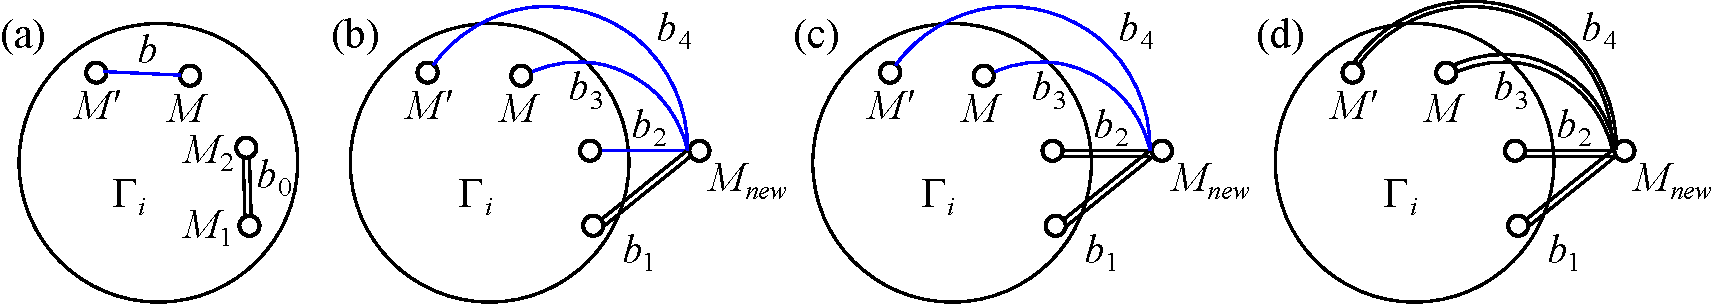
\includegraphics[width=13.5cm]{add_Q8.pdf}}
\end{equation}
Here the graph (a) is obtained from $\cal G$ by replacing $\Iso_{i+1}$ and its two external edges with a $\dashed$ edge $b_0$ between $\cal M_1$ and $\cal M_2$. By the property (iii) of Definition \ref{def seqPDG}, the component $\Gamma_i$ in graph (a) is pre-deterministic. Suppose a pre-deterministic order of the blue solid edges is $e_1\preceq \cdots \preceq e_{\ell-1}\preceq b\preceq e_{\ell+1}\preceq\cdots\preceq e_{k}$. First, by Claim \ref{trivial_graph4}, the edge $b_2$ in the graph (b) of \eqref{graph_add_Q8} is redundant, so we can change it into a $\dashed$ edge and get the graph (c). Second, by Claim \ref{trivial_graph5} (i), the blue solid edges $e_1, \cdots, e_{\ell-1}$ inside $\Gamma_{i}$ can be changed into $\dashed$ edges one by one. Third, by Claim \ref{trivial_graph5} (ii), the edges $b_3$ and $ b_4$ can be changed into $\dashed$ edges according to the order $b_3\preceq b_4$ or $b_4\preceq b_3$, which gives the graph (d) of \eqref{graph_add_Q8}. Finally, by Claim \ref{trivial_graph6}, the blue solid edges $e_{\ell+1},\cdots, e_{k}$ in $\Gamma_{i}$ can be changed into $\dashed$ edges one by one. 
		
In sum, we have shown that the blue solid edges in $\Iso_{i}$ can be changed into $\dashed$ edges one by one according to an order given by the above argument. Hence $\Iso_{i}$ is pre-deterministic. This concludes the case (i) of Lemma \ref{hard lemmQ}.
\end{proof}
	
The cases (ii)--(v) of Lemma \ref{hard lemmQ} are all easier to prove than case (i). We consider them case by case. 
	
\begin{proof}[Proof of Lemma \ref{hard lemmQ}: cases (ii) and (iv)] 
For the case (ii), the statement that $\Iso_{i+1}$ is the maximal isolated subgraph of $\Iso_j$ is trivial. We replace $\Iso_{i+1}$ and its two external edges with a $\dashed$ edge, and get the following graph (a) for the isolated subgraph $\Iso_j$ of \smash{$\wt{\cal G}$}:
\begin{equation} \label{eq_add_Q9}
\parbox[c]{0.9\linewidth}{\center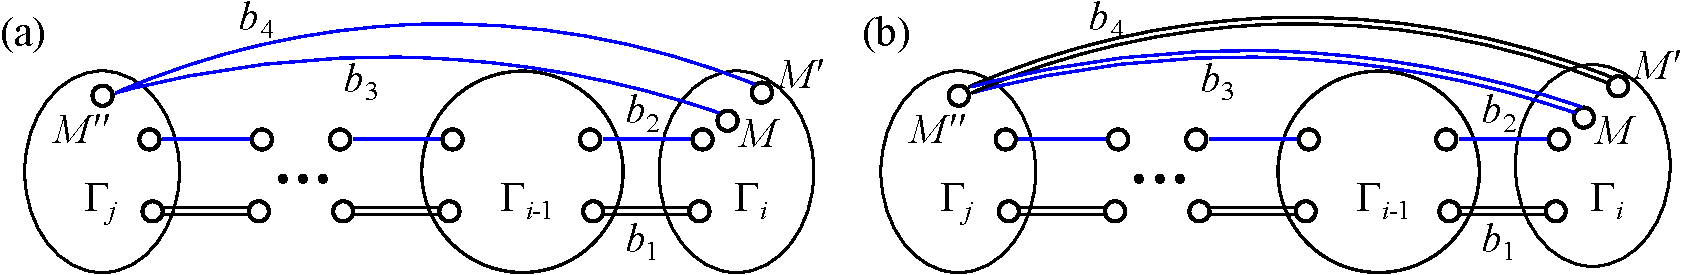
\includegraphics[width=14.5cm]{add_Q9.pdf}}
\end{equation}
By the SPD property of $\cal G$, we know that after replacing the edges $b_3$ and $b_4$ in the graph (a) with a blue solid edge $b:=(\cal M,\cal M')$, the graph component $\Gamma_j$ becomes pre-deterministic. Suppose a pre-deterministic order of blue solid edges in $\Gamma_i$ is $e_1\preceq \cdots \preceq e_{\ell-1}\preceq b\preceq e_{\ell+1}\preceq \cdots\preceq e_{k}$.
% as in the first graph of \eqref{eq_add_Q9}:
%		\begin{equation} %\label{eq_add_Q9}
%			\parbox[c]{0.9\linewidth}{\center
%				\includegraphics[width=15cm]{add_Q9.png}}
%		\end{equation}
%		In the second graph, we replace the edge $b$ with two blue solid edges $b_1$ and $b_2$ between $\Gamma_i$ and $\Gamma_j$ as in case (ii) of Lemma \ref{hard lemmQ}. We want to show this graph is pre-deterministic. 
Then it is trivial to observe that in the graph (a), the edges $e_1, \cdots, e_{\ell-1}, b_3, b_4, e_{\ell+1},\cdots, e_{k}$ can be changed into $\dashed$ edges one by one, which gives the graph (b) of \eqref{eq_add_Q9}. Now if we put $b_3$ into the blue net and $b_4$ into the black net, the subgraph induced on the molecules in $\Gamma_i$ and the molecule $\cal M''$ is doubly connected. By Claim \ref{trivial_graph1}, it is equivalent to look at the quotient graph with this subgraph replaced by a single vertex. The quotient graph has the same structure as the graph (a) of \eqref{graph_adddot2}, which has been shown to be pre-deterministic. This concludes the case (ii) of Lemma \ref{hard lemmQ}.
		
		
%After replacing $\overline I_{i+1}$ with a blue edge $b_1$ and the path $a\to \gamma\to b$ with a blue edge $(a,b)$, the subgraph $I_i$ becomes pre-deterministic. Let the edge $(a,b)$ be the $l$-th edge $b_l$ in the pre-deterministic order. We first change $b_1,\cdots, b_{l-1} $ into $\dashed$ edges one by one. Then the edges $(a,\gamma)$ and $(b,\gamma)$ become redundant, and we can turn them into $\dashed$ edges. Next we change the plus $G$ edges in $I_j$ into $\dashed$ edges according to the following order. We first handle the edges $b_{l+1},b_{l+2},\cdots$ in $\Gamma_i$, then the plus $G$ edge $(x,\al)$ connecting $\Gamma_i$ and $\Gamma_{i-1}$, then the plus $G$ edges in $\Gamma_{i-1}$, then the plus $G$ edge connecting $\Gamma_{i-1}$ and $\Gamma_{i-2}$, and so on until all the plus $G$ edges in $I_j$ are turned into $\dashed$ edges. This concludes case (ii). In fact, since the edges $(a,\gamma)$ and $(b,\gamma)$ are turned into $\dashed$ edges in a relatively earlier stage, the proof of case (ii) is a little bit easier than the proof for case (i). 
		
		
For the case (iv), we replace $\Iso_{i+2}$ and its two external edges with a $\dashed$ edge, and get the following graph (a) for the isolated subgraph $\Iso_j$ of $\wt{\cal G}$:
%Then after replacing $\Iso_{i+1}$ and its two external edges with a $\dashed$ edge, we get the second graph in the following figure:
\begin{equation} \label{eq_add_Q10}
\parbox[c]{0.9\linewidth}{\center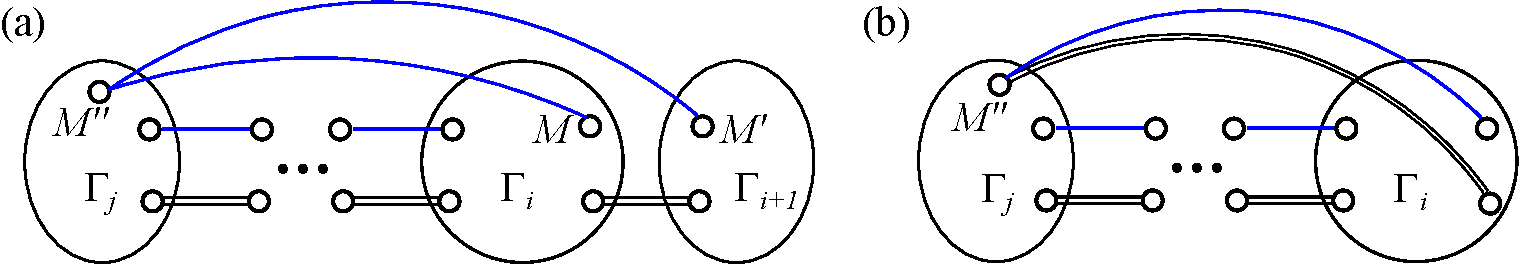
\includegraphics[width=13cm]{add_Q10.pdf}}
\end{equation}
The statement that $\Iso_{i+1}$ is the maximal isolated subgraph of $\Iso_j$ is trivial. Then we replace $\Iso_{i+1}$ and its two external edges with a $\dashed$ edge, and get the graph (b) in \eqref{eq_add_Q10}. Again this graph has the same structure as the graph (a) of \eqref{graph_adddot2}, which has been shown to be pre-deterministic. Hence we conclude the case (iv) of Lemma \ref{hard lemmQ}.
%First, it is easy to see that the blue solid edge between $\cal M$ and $\cal M''$ is redundant in the second graph of \eqref{eq_add_Q10}. We can change it into a $\dashed$ edge and obtain the third graph of \eqref{eq_add_Q10}. We see that it has the same structure as the third graph of \eqref{eq_add_Q9}. Hence the same proof for case (ii) concludes case (iv).
\end{proof}


The proofs of cases (iii) and (v) of Lemma \ref{hard lemmQ} use the following two claims. 
	
	
\begin{claim}\label{trivial_graph2}
Given a doubly connected graph $\cal G$, we construct a new graph $\cal G_{new}$ as follows: 
\begin{center}
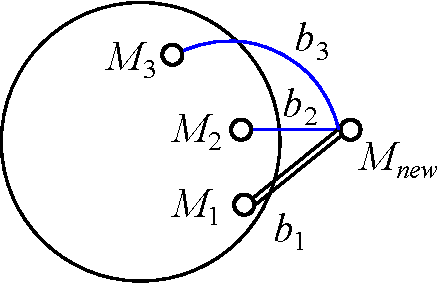
\includegraphics[width=4cm]{add_Q11.pdf}
\end{center}		
More precisely, we create a new molecule $\cal M_{new}$. Given any three molecules $\cal M_1$, $\cal M_2$ and $\cal M_3$ in $\cal G$, we add a $\dashed$ edge $b_1$ between $\cal M_{new}$ and $\cal M_1$, a blue solid edge $b_2$ between $\cal M_{new}$ and $\cal M_2$, and a blue solid edge $b_3$ between $\cal M_{new}$ and $\cal M_3$. Then the blue solid edges $b_2$ and $b_3$ are both redundant in $\cal G_{new}$.
\end{claim}
%	\begin{proof}
%		We have the following graph:
%		\begin{center}
%			\includegraphics[width=4cm]{add_Q11.png}
%		\end{center}
%		Let the black net and blue net in $\cal G$ be $\cal B_1$ and $\cal B_2$, respectively. Then $\cal B_1\cup \{b_1\}$ is a blue net in $\cal G_{new}$, and $\cal B_2\cup \{b_2\}$ is a blue net in $\cal G_{new}$. Hence $b_3$ is redundant. Similarly, $\cal B_2\cup \{b_3\}$ is another blue net in $\cal G_{new}$. Hence $b_2$ is redundant.
%	\end{proof}
	
\begin{claim}\label{trivial_graph7}
Given a doubly connected graph $\cal G$, we construct a new graph $\cal G_{new}$ as follows: 
\begin{center}
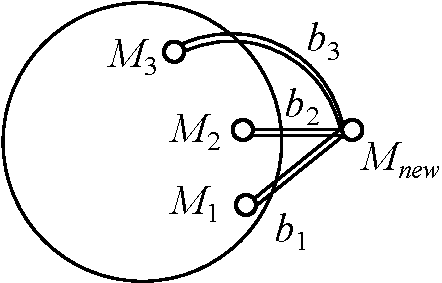
\includegraphics[width=4cm]{add_Q13.pdf}
\end{center}
More precisely, we create a new molecule $\cal M_{new}$, replace a $\dashed$ edge $b_0=(\cal M_1,\cal M_2)$ in $\cal G$ with two $\dashed$ edges $b_1$ between $\cal M_1$ and $\cal M_{new}$ and $b_2$ between $\cal M_2$ and $\cal M_{new}$, and add a $\dashed$ edge $b_3$ between $\cal M_{new}$ and a molecule $\cal M_3$ in $\cal G$. If a blue solid edge is redundant in $\cal G$, it is also redundant in $\cal G_{new}$.
\end{claim}
%	\begin{proof}
%		We have the following graph:
%		\begin{center}
%			\includegraphics[width=7cm]{add_Q13.png}
%		\end{center}
%		Let the black net and blue net in $\cal G$ be $\cal B_1$ and $\cal B_2$,  so that $b$ is redundant. If $b_0$ is used in the black net in $\cal G$ in order for $b$ to be redundant, then we put $b_0$ and $b_1$ into the black net and $b_3$ into the blue net. It is easy to check that $\cal B_1\cup \{b_1, b_2\}\setminus \{b_0\}$ and $\cal B_2\cup \{b_3\}\setminus \{b\}$ are the black and blue nets in $\cal G_{new}$, which shows that $b$ is redundant in $\cal G_{new}$. 
%		On the other hand, if $b_0$ is used in the blue net in $\cal G$ in order for $b$ to be redundant, then  we put $b_0$ and $b_1$ into the blue net and $b_3$ into the black net. It is easy to check that $\cal B_1\cup \{b_3\}$ and $\cal B_2\cup \{b_1, b_2\}\setminus \{b\}$ are the black and blue nets in $\cal G_{new}$, which shows that $b$ is redundant in $\cal G_{new}$. 
%	\end{proof}
The proofs of the above two claims are simple, so we omit the details. 	
	
\begin{proof}[Proof of Lemma \ref{hard lemmQ}: cases (iii) and (v)] 
The case (v) can be regarded as a special case of the case (iii). For the case (iii), it is trivial to show that $\Iso_{i+1}$ is the maximal isolated subgraph of $\Iso_i$, and $\Iso_{j+1}$ is the maximal isolated subgraph of $\Iso_{i+1}$. We replace $\Iso_{j+1}$ and its two external edges with a $\dashed$ edge and get the following graph (a) for the isolated subgraph $\Iso_{i+1}$: 
\begin{equation} \label{eq_add_Q12}
	\parbox[c]{0.8\linewidth}{\center
		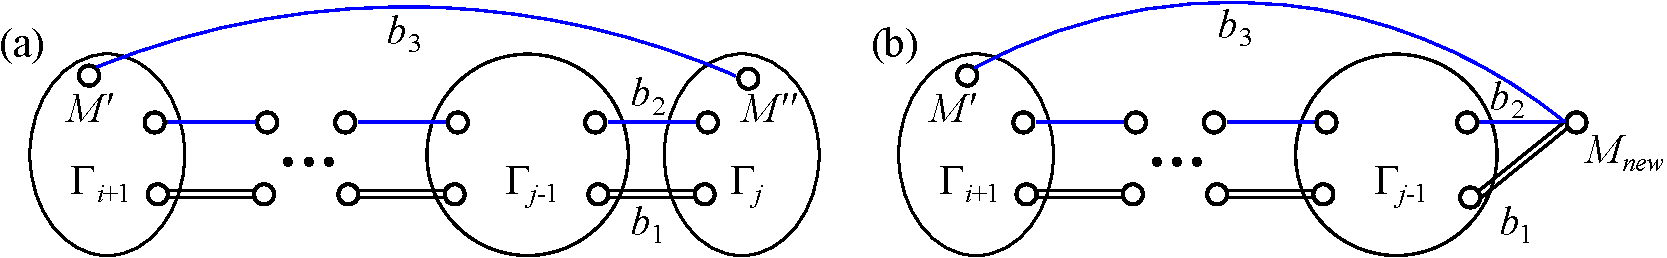
\includegraphics[width=14cm]{add_Q12.pdf}}
\end{equation}
%		\begin{equation} %\label{eq_add_Q12}
%			\parbox[c]{0.8\linewidth}{\center
%				\includegraphics[width=14cm]{add_Q12.png}}
%		\end{equation}
By the SPD property of $\cal G$, the component $\Gamma_j$ in the graph (a) of \eqref{eq_add_Q12} is pre-deterministic, so we can change its blue solid edges into $\dashed$ edges one by one. Then by Claim \ref{trivial_graph1}, we can replace $\Gamma_j$ with a single molecule and get the graph (b) of \eqref{eq_add_Q12}. Now by Claim \ref{trivial_graph2}, both $b_2$ and $b_3$ are redundant, so we can change them into $\dashed$ edges. % as in the third graph of \eqref{eq_add_Q12}. 
Next by Claim \ref{trivial_graph7}, we can change the blue solid edges in $\Gamma_{j-1}$ into $\dashed$ edges one by one. In the resulting graph, the subgraph induced on the molecules in $\Gamma_{j-1}$ and the molecule $\cal M_{new}$ is a doubly connected subgraph (the subgraph induced on $\Gamma_{j-1}$ is doubly connected by the fact stated after Claim \ref{trivial_graph3}, and $\cal M_{new}$ is connected to it through the $\dashed$ edges $b_1$ and $b_2$), so by Claim \ref{trivial_graph1} we can replace them with a single molecule and get a graph that is similar to the graph (b) of \eqref{eq_add_Q12}. Repeating the above argument, we can show that the blue solid edges in $\Iso_{i+1}$ can be changed into $\dashed$ edges one by one according to some order. Hence $\Iso_{i+1}$ is pre-deterministic, which concludes the case (iii) of Lemma \ref{hard lemmQ}.
%In this case, we notice that $I_{i+1}$ is still an isolated subgraph. Moreover, we change the plus $G$ edges in $I_{i+1}$ into $\dashed$ edges according to the following order. We first handle the edges in $\Gamma_j$ according to the pre-deterministic order, then the plus $G$ edge $(x,\al)$ connecting $\Gamma_{j}$ and $\Gamma_{j-1}$, then the plus $G$ edges in $\Gamma_{j-1}$, then the plus $G$ edge connecting $\Gamma_{j-1}$ and $\Gamma_{j-2}$, and so on until all the plus $G$ edges in $I_{i+1}$ are turned into $\dashed$ edges except for the edge $(b,\gamma)$. Now it is easy to see that edge $(b,\gamma)$ is redundant, because without it the blue net in $I_{i+1}$ is connected to $\Gamma_i$ through edge $(a,\gamma)$. 
\end{proof}



%\subsection*{Data availability statement}  Not applicable. %(data transparency)

%\bibliographystyle{abbrv}
%\bibliography{band_bib}
% \bib, bibdiv, biblist are defined by the amsrefs package.
\begin{bibdiv}
	\begin{biblist}
		
		\bib{Anderson}{article}{
			author={Anderson, P.~W.},
			title={Absence of diffusion in certain random lattices},
			date={1958},
			journal={Phys. Rev.},
			volume={109},
			pages={1492\ndash 1505},
		}
		
		\bib{BaoErd2015}{article}{
			author={Bao, Z.},
			author={Erd{\H{o}}s, L.},
			title={Delocalization for a class of random block band matrices},
			date={2017},
			journal={Probab. Theory Relat. Fields},
			volume={167},
			number={3},
			pages={673\ndash 776},
		}
		
		\bib{PB_review}{incollection}{
			author={Bourgade, P.},
			title={Random band matrices},
			date={2018},
			booktitle={Proceedings of the {I}nternational {C}ongress of
				{M}athematicians},
			pages={2759\ndash 2783},
		}
		
		\bib{BouErdYauYin2017}{article}{
			author={Bourgade, P.},
			author={Erd{\H o}s, L.},
			author={Yau, H.-T.},
			author={Yin, J.},
			title={Universality for a class of random band matrices},
			date={2017},
			journal={Advances in Theoretical and Mathematical Physics},
			volume={21},
			number={3},
			pages={739\ndash 800},
		}
		
		\bib{PartII}{article}{
			author={Bourgade, P.},
			author={Yang, F.},
			author={Yau, H.-T.},
			author={Yin, J.},
			title={Random band matrices in the delocalized phase, {II}: Generalized
				resolvent estimates},
			date={2019},
			journal={J. Stat. Phys.},
			volume={174},
			number={6},
			pages={1189\ndash 1221},
		}
		
		\bib{PartI}{article}{
			author={Bourgade, P.},
			author={Yau, H.-T.},
			author={Yin, J.},
			title={Random band matrices in the delocalized phase, {I}: Quantum
				unique ergodicity and universality},
			date={2020},
			journal={Comm. Pure Appl. Math.},
			volume={73},
			number={7},
			pages={1526\ndash 1596},
		}
		
		\bib{ConJ-Ref2}{article}{
			author={Casati, G.},
			author={Guarneri, I.},
			author={Izrailev, F.},
			author={Scharf, R.},
			title={Scaling behavior of localization in quantum chaos},
			date={1990Jan},
			journal={Phys. Rev. Lett.},
			volume={64},
			pages={5\ndash 8},
		}
		
		\bib{ConJ-Ref1}{article}{
			author={Casati, G.},
			author={Molinari, L.},
			author={Izrailev, F.},
			title={Scaling properties of band random matrices},
			date={1990Apr},
			journal={Phys. Rev. Lett.},
			volume={64},
			pages={1851\ndash 1854},
		}
		
		\bib{ErdKno2013}{article}{
			author={Erd{\H{o}}s, L.},
			author={Knowles, A.},
			title={Quantum diffusion and delocalization for band matrices with
				general distribution},
			date={2011},
			journal={Ann. Henri Poincar\'e},
			volume={12},
			number={7},
			pages={1227\ndash 1319},
		}
		
		\bib{ErdKno2011}{article}{
			author={Erd{\H{o}}s, L.},
			author={Knowles, A.},
			title={Quantum diffusion and eigenfunction delocalization in a random
				band matrix model},
			date={2011},
			journal={Comm. Math. Phys.},
			volume={303},
			number={2},
			pages={509\ndash 554},
		}
		
		\bib{EKY_Average}{article}{
			author={Erd{\H o}s, L.},
			author={Knowles, A.},
			author={Yau, H.-T.},
			title={Averaging fluctuations in resolvents of random band matrices},
			date={2013},
			journal={Ann. Henri Poincar\'e},
			volume={14},
			pages={1837\ndash 1926},
		}
		
		\bib{delocal}{article}{
			author={Erd{\H{o}}s, L.},
			author={Knowles, A.},
			author={Yau, H.-T.},
			author={Yin, J.},
			title={Delocalization and diffusion profile for random band matrices},
			date={2013},
			journal={Comm. Math. Phys.},
			volume={323},
			number={1},
			pages={367\ndash 416},
		}
		
		\bib{Semicircle}{article}{
			author={Erd{\H{o}}s, L.},
			author={Knowles, A.},
			author={Yau, H.-T.},
			author={Yin, J.},
			title={The local semicircle law for a general class of random matrices},
			date={2013},
			journal={Elect. J. Prob.},
			volume={18},
			number={59},
			pages={1\ndash 58},
		}
		
		\bib{ErdYauYin2012Univ}{article}{
			author={Erd{\H{o}}s, L.},
			author={Yau, H.-T.},
			author={Yin, J.},
			title={Bulk universality for generalized {W}igner matrices},
			date={2012},
			journal={Probab. Theory Relat. Fields},
			volume={154},
			number={1-2},
			pages={341\ndash 407},
		}
		
		\bib{ConJ-Ref4}{article}{
			author={Feingold, M.},
			author={Leitner, D.~M.},
			author={Wilkinson, M.},
			title={Spectral statistics in semiclassical random-matrix ensembles},
			date={1991Feb},
			journal={Phys. Rev. Lett.},
			volume={66},
			pages={986\ndash 989},
		}
		
		\bib{fy}{article}{
			author={Fyodorov, Y.~V.},
			author={Mirlin, A.~D.},
			title={Scaling properties of localization in random band matrices: A
				$\sigma$-model approach.},
			date={1991},
			journal={Phys. Rev. Lett.},
			volume={67},
			pages={2405\ndash 2409},
		}
		
		\bib{HeMa2018}{article}{
			author={He, Y.},
			author={Marcozzi, M.},
			title={Diffusion profile for random band matrices: A short proof},
			date={2019},
			journal={J. Stat. Phys.},
			volume={177},
			number={4},
			pages={666\ndash 716},
			url={https://doi.org/10.1007/s10955-019-02385-2},
		}
		
		\bib{PelSchShaSod}{article}{
			author={Peled, R.},
			author={Sodin, S.},
			author={Schenker, J.},
			author={Shamis, M.},
			title={{On the Wegner Orbital Model}},
			date={201707},
			journal={International Mathematical Research Notices},
		}
		
		\bib{Sch2009}{article}{
			author={Schenker, J.},
			title={Eigenvector localization for random band matrices with power law
				band width},
			date={2009},
			journal={Comm. Math. Phys.},
			volume={290},
			pages={1065\ndash 1097},
		}
		
		\bib{SchMT}{article}{
			author={Shcherbina, M.},
			author={Shcherbina, T.},
			title={Characteristic polynomials for 1d random band matrices from the
				localization side},
			date={2017},
			journal={Comm. Math. Phys.},
			volume={351},
			number={3},
			pages={1009\ndash 1044},
		}
		
		\bib{Sch3}{article}{
			author={Shcherbina, M.},
			author={Shcherbina, T.},
			title={Universality for 1d random band matrices: Sigma-model
				approximation},
			date={2018},
			journal={J. Stat. Phys.},
			volume={172},
			number={2},
			pages={627\ndash 664},
			url={https://doi.org/10.1007/s10955-018-1969-1},
		}
		
		\bib{1Dchara}{article}{
			author={Shcherbina, Mariya},
			author={Shcherbina, Tatyana},
			title={Universality for 1d random band matrices},
			date={2021},
			journal={Comm. Math. Phys.},
			volume={385},
			number={2},
			pages={667\ndash 716},
		}
		
		\bib{Sch1}{article}{
			author={Shcherbina, T.},
			title={On the second mixed moment of the characteristic polynomials of
				1d band matrices},
			date={2014},
			journal={Comm. Math. Phys.},
			volume={328},
			pages={45\ndash 82},
		}
		
		\bib{Sch2014}{article}{
			author={Shcherbina, T.},
			title={Universality of the local regime for the block band matrices with
				a finite number of blocks},
			date={2014},
			journal={J. Stat. Phys.},
			volume={155},
			pages={466\ndash 499},
		}
		
		\bib{Sch2}{article}{
			author={Shcherbina, T.},
			title={Universality of the second mixed moment of the characteristic
				polynomials of the 1d band matrices: Real symmetric case},
			date={2015},
			journal={J. Math. Phys.},
			volume={56},
		}
		
		\bib{Sod2010}{article}{
			author={Sodin, S.},
			title={The spectral edge of some random band matrices},
			date={2010},
			journal={Ann. of Math.},
			volume={173},
			number={3},
			pages={2223\ndash 2251},
		}
		
		\bib{Spencer3}{article}{
			author={Spencer, T.},
			title={Duality, statistical mechanics and random matrices},
			journal={Current Developments in Mathematics},
			volume={2012},
			pages={229\ndash 260},
		}
		
		\bib{Spencer2}{incollection}{
			author={Spencer, T.},
			title={Random banded and sparse matrices},
			date={2011},
			booktitle={Oxford handbook of random matrix theory},
			editor={Akemann, G.},
			editor={Baik, J.},
			editor={Francesco, P.~Di},
			publisher={Oxford University Press},
			address={New York},
		}
		
		\bib{Spencer1}{incollection}{
			author={Spencer, T.},
			title={{SUSY} statistical mechanics and random band matrices},
			date={2012},
			booktitle={Quantum many body systems},
			series={Lecture Notes in Mathematics, vol 2051},
			publisher={Springer},
			address={Berlin, Heidelberg},
		}
		
		\bib{Wigner}{article}{
			author={Wigner, E.~P.},
			title={Characteristic vectors of bordered matrices with infinite
				dimensions},
			date={1955},
			journal={Ann. of Math.},
			volume={62},
			number={3},
			pages={548\ndash 564},
		}
		
		\bib{ConJ-Ref6}{article}{
			author={Wilkinson, M.},
			author={Feingold, M.},
			author={Leitner, D.~M.},
			title={Localization and spectral statistics in a banded random matrix
				ensemble},
			date={1991},
			journal={Journal of Physics A: Mathematical and General},
			volume={24},
			number={1},
			pages={175},
		}
		
		\bib{PartI_high}{article}{
			author={Yang, F.},
			author={Yau, H.-T.},
			author={Yin, J.},
			title={Delocalization and quantum diffusion of random band matrices in
				high dimensions {I}: self-energy renormalization},
			date={2021},
			journal={arXiv:2104.12048},
		}
		
		\bib{PartIII}{article}{
			author={Yang, F.},
			author={Yin, J.},
			title={Random band matrices in the delocalized phase, {III}: averaging
				fluctuations},
			date={2021},
			journal={Probab. Theory Relat. Fields},
			volume={179},
			pages={451\ndash 540},
		}
		
	\end{biblist}
\end{bibdiv}


\end{document}




  
   

